\documentclass[11pt,oneside]{article}
\usepackage{fontspec,xeCJK,graphicx,tikz,geometry,titlesec,fancyhdr,hyperref,bookmark,amsmath,lmodern,newunicodechar,indentfirst,xurl}
\usepackage{setspace,tocloft,tabularx,booktabs}
\usepackage{caption,placeins}
\captionsetup{font=small,skip=6pt,singlelinecheck=false,justification=raggedright}
\newcommand{\BookTableStyle}{\setstretch{1}\fontsize{9}{12}\selectfont\setlength{\tabcolsep}{4pt}\renewcommand{\arraystretch}{1.2}}
\newcommand{\BookFloatNotes}[1]{\par\vspace{4pt}{\setstretch{1}\fontsize{9}{12}\selectfont\raggedright\noindent #1\par}}
% ISO B5，单面排版，左右边距相同。
\newcommand{\BookWidth}{176mm}
\newcommand{\BookHeight}{250mm}

\geometry{paperwidth=\BookWidth,paperheight=\BookHeight,left=20mm,right=20mm,top=22mm,bottom=24mm,headheight=0pt,footskip=11mm}
\IfFontExistsTF{SimSun}{\setCJKmainfont{SimSun}\newCJKfontfamily\bookfang{FangSong}\newCJKfontfamily\bookhei{SimHei}}{%
\IfFileExists{/mnt/c/Windows/Fonts/simsun.ttc}{\setCJKmainfont[Path=/mnt/c/Windows/Fonts/]{simsun.ttc}\newCJKfontfamily\bookfang[Path=/mnt/c/Windows/Fonts/]{simfang.ttf}\newCJKfontfamily\bookhei[Path=/mnt/c/Windows/Fonts/]{simhei.ttf}}{\setCJKmainfont{FandolSong-Regular}\newCJKfontfamily\bookfang{FandolFang-Regular}\newCJKfontfamily\bookhei{FandolHei-Regular}}}
\IfFontExistsTF{Times New Roman}{\setmainfont{Times New Roman}}{\setmainfont{TeX Gyre Termes}}
\newfontfamily\symbolfont{SimSun}
\newunicodechar{①}{{\symbolfont ①}}
\newunicodechar{②}{{\symbolfont ②}}
\newunicodechar{③}{{\symbolfont ③}}
\newunicodechar{△}{\ensuremath{\triangle}}
\newunicodechar{□}{\ensuremath{\square}}
\IfFileExists{/mnt/c/Windows/Fonts/simsunb.ttf}{\setCJKfallbackfamilyfont{rm}[Path=/mnt/c/Windows/Fonts/]{simsunb.ttf}}{}
% 独立引文使用楷体；六角括号内的作者注使用仿宋，分组结束后恢复引文字体。
\IfFontExistsTF{KaiTi}{\newCJKfontfamily\bookkai{KaiTi}}{%
\IfFileExists{/mnt/c/Windows/Fonts/simkai.ttf}{\newCJKfontfamily\bookkai[Path=/mnt/c/Windows/Fonts/]{simkai.ttf}}{\newCJKfontfamily\bookkai{FandolKai-Regular}}}
\newcommand{\AuthorNote}[1]{{\bookfang #1}}
\hypersetup{unicode=true,hidelinks,pageanchor=false,pdftitle={康熙的红票：B5重排校对稿},pdfauthor={孙立天}}
\pdfstringdefDisableCommands{\def\quad{ }}
\urlstyle{same}
\setlength{\parindent}{2em}\setlength{\parskip}{.3\baselineskip}
\setstretch{1.5}\raggedbottom
\setlength{\emergencystretch}{2em}
\fancyhf{}
\fancyfoot[L]{\bookfang\small\nouppercase{\leftmark}}
\fancyfoot[R]{\small\thepage}
\renewcommand{\headrulewidth}{0pt}
\renewcommand{\footrulewidth}{0pt}
\pagestyle{fancy}
\fancypagestyle{plain}{\fancyhf{}\fancyfoot[L]{\bookfang\small\nouppercase{\leftmark}}\fancyfoot[R]{\small\thepage}\renewcommand{\headrulewidth}{0pt}\renewcommand{\footrulewidth}{0pt}}
\renewcommand{\sectionmark}[1]{}
\renewcommand{\subsectionmark}[1]{}
\newcommand{\BookChinese}[1]{\ifcase#1\or 一\or 二\or 三\or 四\or 五\or 六\or 七\or 八\or 九\or 十\fi}
\renewcommand{\thesection}{第\BookChinese{\value{section}}章}
\renewcommand{\thesubsection}{\arabic{section}.\arabic{subsection}}
\renewcommand{\thepart}{第\BookChinese{\value{part}}部分}
\titleformat{\part}[display]{\centering\bookhei\LARGE}{\thepart}{1em}{}
\titleformat{\section}{\bookhei\fontsize{17}{23}\selectfont}{\thesection}{1em}{}
\titleformat{\subsection}{\bookhei\fontsize{12}{17}\selectfont}{\thesubsection}{1em}{}
\titlespacing*{\section}{0pt}{0pt}{18pt}\titlespacing*{\subsection}{0pt}{16pt}{9pt}
\newcommand{\BookUnnumbered}[1]{\section*{#1}\phantomsection\addcontentsline{toc}{section}{#1}}
\newcommand{\BookSubUnnumbered}[1]{\subsection*{#1}\phantomsection\addcontentsline{toc}{subsection}{#1}}
% 正文上标与书后编号使用同一语义标识；注释正文保持悬挂缩进。
\newcommand{\NoteRef}[2]{\textsuperscript{\hyperlink{note-#1-#2}{\normalfont #2}}}
\newcommand{\NoteChapter}[1]{\subsection*{#1}}
\newcommand{\NoteEntry}[3]{\par\noindent\hangindent=2.5em\hangafter=1\makebox[2.5em][l]{\hypertarget{note-#1-#2}{#2}}#3\par}
% 目录的页码由编译生成，章、节都不使用首行缩进。
\setcounter{tocdepth}{2}
\renewcommand{\contentsname}{目\quad 录}
\renewcommand{\cfttoctitlefont}{\hfill\bookhei\Large}
\renewcommand{\cftaftertoctitle}{\hfill}
\setlength{\cftbeforetoctitleskip}{0pt}
\setlength{\cftaftertoctitleskip}{22pt}
\setlength{\cftpartindent}{0pt}\setlength{\cftpartnumwidth}{5.5em}
\setlength{\cftsecindent}{0pt}\setlength{\cftsecnumwidth}{4.5em}
\setlength{\cftsubsecindent}{0pt}\setlength{\cftsubsecnumwidth}{3em}
\renewcommand{\cftpartfont}{\bookhei}\renewcommand{\cftpartpagefont}{\normalfont}
\renewcommand{\cftsecfont}{\bookhei}\renewcommand{\cftsecpagefont}{\normalfont}
\renewcommand{\cftsubsecfont}{\normalfont\small}\renewcommand{\cftsubsecpagefont}{\normalfont\small}
\renewcommand{\cftpartleader}{\cftdotfill{\cftdotsep}}
\renewcommand{\cftsecleader}{\cftdotfill{\cftdotsep}}
\renewcommand{\cftsecafterpnum}{\par\nobreak}
\setlength{\cftbeforepartskip}{14pt}\setlength{\cftbeforesecskip}{7pt}\setlength{\cftbeforesubsecskip}{2pt}
\newcommand{\PictureContentsEntry}[2]{\par\noindent #1\nobreak\leaders\hbox to .65em{\hss.\hss}\hfill\nobreak\makebox[2em][r]{\pageref{#2}}\par}
% 原扫描对照入口也使用 B5；图片等比放入版心。
\newcommand{\OriginalPage}[1]{\clearpage\noindent\includegraphics[width=\linewidth,height=\textheight,keepaspectratio]{scanned-version/#1.jpg}\par}

\begin{document}
\clearpage\markboth{卷首、目录与序}{卷首、目录与序}
% 卷首、目录与序
% 原书页码：无印刷页码；版权页／图书在版编目表。
\begingroup\small\setstretch{1.2}\setlength{\parskip}{0pt}
\noindent\begin{minipage}{\linewidth}
\centering
\begin{minipage}{.91\linewidth}
\centering 图书在版编目（CIP）数据\par\vspace{1.4em}
\raggedright\setlength{\parindent}{2em}
康熙的红票：全球化中的清朝／孙立天著．—北京：商务印书馆，2024（2026.2重印）\par
\vspace{.6em}ISBN 978-7-100-23424-5\par
\vspace{.9em}I.①康…\quad Ⅱ.①孙…\quad Ⅲ.①中国历史—研究—清代\quad Ⅳ.①K249.07\par
\vspace{.7em}中国国家版本馆CIP数据核字（2024）第044788号\par
\end{minipage}\par
\vspace{2.4em}
权利保留，侵权必究。\par
\vspace{3em}
{\bookhei\Large 康熙的红票}\par\vspace{.5em}
{\normalsize 全球化中的清朝}\par\vspace{.6em}
孙立天\quad 著\par\vspace{1.3em}
\begin{tabularx}{\linewidth}{@{}Xr@{}}
\toprule[.5pt]
\multicolumn{2}{c}{商务印书馆出版}\\
\multicolumn{2}{c}{（北京王府井大街36号\quad 邮政编码100710）}\\
\multicolumn{2}{c}{商务印书馆发行}\\
\multicolumn{2}{c}{北京中科印刷有限公司印刷}\\
\multicolumn{2}{c}{ISBN 978-7-100-23424-5}\\
\midrule[.5pt]
2024年3月第1版 & 开本880×1240\quad 1/32\\
2026年2月北京第11次印刷 & 印张12½\quad 插页2\\
\multicolumn{2}{c}{定价：78.00元}
\end{tabularx}
\end{minipage}\par\endgroup
% 原书页码：无印刷页码；原目录改为自动目录，增加节标题页码。
\clearpage\markboth{目录}{目录}
\begingroup\setstretch{1.15}\setlength{\parskip}{0pt}\tableofcontents\endgroup
% 原书页码：无印刷页码；原目录续页已合并为自动目录。
% 原书页码：无印刷页码；图片目录，页码指向重排后的图版。
\clearpage\markboth{图片目录}{图片目录}
{\centering\bookhei\Large 图片目录\par}\vspace{18pt}
\begingroup\small\setstretch{1.25}\setlength{\parskip}{.5em}
\PictureContentsEntry{图0.1 康熙御批红票草稿}{fig-14-0}
\PictureContentsEntry{卷首图1 康熙坐像}{fig-front-kangxi}
\PictureContentsEntry{卷首图2 “中国皇帝外出巡幸”挂毯}{fig-front-tapestry}
\PictureContentsEntry{图3.1 南怀仁石料牵引图}{fig-105-0}
\PictureContentsEntry{图3.2 南怀仁车模型图}{fig-107-0}
\PictureContentsEntry{图3.3 牛顿1688年提出的蒸汽车构想图}{fig-107-1}
\PictureContentsEntry{图4.1 内务府发于传教士的印票}{fig-145-0}
\PictureContentsEntry{图4.2 康熙过问西洋人打架案谕旨}{fig-148-0}
\PictureContentsEntry{图4.3 清初北京教堂位置图}{fig-154-0}
\PictureContentsEntry{图4.4 故宫档案藏治疗教皇使节多罗药方}{fig-165-0}
\PictureContentsEntry{图5.1 康熙批改闵明我劝多罗信}{fig-216-0}
\PictureContentsEntry{图6.1 康熙批注教皇禁约}{fig-254-0}
\PictureContentsEntry{图6.2 艾若瑟墓碑正面碑文}{fig-259-0}
\PictureContentsEntry{图6.3 艾若瑟墓碑背面碑文}{fig-260-0}
\PictureContentsEntry{图8.1 康熙谈论代数谕旨}{fig-311-0}
\PictureContentsEntry{图8.2 鲁本斯绘金尼阁着儒服全身像}{fig-323-0}
\endgroup\clearpage\markboth{序}{序}
% 原书页码：i；标题
\BookUnnumbered{序}
\par
% 原书页码：i；段落
2019年北京春季艺术品拍卖会上，出现了一张康熙时期发去欧洲%
的谕令。拍卖时的名字是《康熙帝寄西洋众人谕》。这件拍品不是康%
熙亲笔谕旨，而是一份印刷品，宽39厘米，长93厘米，于1716年%
由康熙内务府以公开信形式印刷出来，命广东官员发放给欧洲来的商%
船，让他们带回欧洲。这份公开信印刷出来呈朱红色，历史上又称“红%
票”，英文世界，称为“Red Manifesto”。%
\par
% 原书页码：i；段落
红票内容用汉文、满文和拉丁文三种文字印出。其中汉文部分内%
容是：%
\par
% 原书页码：i–ii；段落（跨页续段）
{\bookkai 武英殿等处监修书官伊都立、王道化、赵昌等字寄与自西洋来}%
{\bookkai 的众人。我等谨遵旨于康熙四十五年已曾差西洋人龙安国、薄贤士，}%
{\bookkai 四十七年差西洋人艾若瑟、陆若瑟，奉旨往西洋去了。至今数年，}%
{\bookkai 不但没有信来，所以难辨真假。又有乱来之信，因此与鄂罗斯的人}%
{\bookkai 又带信去，想是到去了。必竟我等差去人回时，事情都明白之后，}%
{\bookkai 方可信得。若是我等差去之人不回，无真凭据，虽有甚么书信，总}%
{\bookkai 信不得。因此，唯恐书信不通，写此字，兼上西洋字刊刻，用广东}%
{\bookkai 巡抚院印，书不封缄，凡来的众西洋人，多发与带去。康熙五十五}%
{\bookkai 年九月十七日。}%
\par
% 原书页码：ii；段落
文字的内容很直白，就是康熙向欧洲陈述一个事实，说他在1706年%
（康熙四十五年）和1708年（康熙四十七年）派了两组人到西洋去，%
现在人都没有回来。除了一些各方面不知真假传回来的消息，他派出%
去的人并没有正式文书寄回。%
\par
% 原书页码：ii；段落
这是一封印刷品，按理说价值不大。但拍卖前，拍卖行给出的估%
价是70万到80万元。拍卖行估到这个价位，显然是做过功课的。在%
拍品介绍的底部，提到红票只在欧美十来所图书馆有馆藏，在中国内%
地（大陆）与香港、台湾地区尚未发现过该票，在华语地区是第一次%
出现。%
\par
% 原书页码：ii–iii；段落（跨页续段）
红票受到关注，也是近二十年来的事。长期以来，红票里面提到%
的“事情明白之后”是什么事情，康熙为什么发这张红票到欧洲，都%
是个谜。因为大清所有官修史书都没有提到过这张红票，与之相关的%
事件也完全没有记录。2011年牛津大学图书馆中国古籍部主管大卫·海%
里威（David Helliwell）在网上分享了一段他与红票的故事。海里威说，%
早在1970年代，他就在牛津一座书库中看到过一张红票，当时是卷%
起来和一个木板绑在一起的。上面只是简单有个库存编号，也就表示%
前任馆员们都不知道这张红票的历史，不知道应该把它归到哪里去。%
当时海里威打开看后也没有头绪，又把它原封不动放回了原位。一直%
到1992年，他去参观法国国家图书馆举办的中西印刷文物展的时候，%
展出的一张红票让他回想起十几年前在牛津书库里见过的那张。展出%
中，关于红票的简单历史脉络已经被法国国家图书馆馆员整理了出来。%
海里威回去后，很快就找到了牛津书库中的那张红票。当他再次把卷%
起来的红票打开，给红票做相应的索引介绍的时候，发现红票背面有%
很浅的铅笔印记“F. Douce”。海里威说这表示红票是古籍收藏家法朗%
士·戴希（Francis Douce，1757—1834）捐给牛津的，也就是说这张%
红票在牛津书库里放了一百多年，一直没人知道其来历背景。海里威%
把他发现这张红票的经历写出来发到网上，很快收到世界各地发来的%
消息，告诉他还有哪些地方也藏有红票。经过统计，现在世界各地有%
18张红票，它们是：%
\par
% 原书页码：iii；段落
1. 巴伐利亚州立图书馆，慕尼黑%
\par
% 原书页码：iii；段落
2. 赫尔佐格·奥古斯特图书馆，沃尔芬比特尔（副本1）%
\par
% 原书页码：iii；段落
3. 赫尔佐格·奥古斯特图书馆，沃尔芬比特尔（副本2）%
\par
% 原书页码：iii；段落
4. 柏林国立图书馆普鲁士文化遗产%
\par
% 原书页码：iii；段落
5. 牛津大学博德利图书馆%
\par
% 原书页码：iii；段落
6. 大英图书馆，伦敦%
\par
% 原书页码：iii；段落
7. 剑桥大学图书馆%
\par
% 原书页码：iii；段落
8. 伦敦木版基金会%
\par
% 原书页码：iii；段落
9. 法国国家图书馆，巴黎%
\par
% 原书页码：iii；段落
10. 莱顿汉学研究所%
\par
% 原书页码：iii；段落
11. 梵蒂冈使徒书院，梵蒂冈城%
\par
% 原书页码：iii；段落
12. 斯德哥尔摩皇家图书馆%
\par
% 原书页码：iv；段落
13. 利玛窦研究所档案馆，波士顿学院%
\par
% 原书页码：iv；段落
14. 印第安纳大学礼来图书馆%
\par
% 原书页码：iv；段落
15. 康奈尔大学图书馆%
\par
% 原书页码：iv；段落
16. 东京私人收藏%
\par
% 原书页码：iv；段落
17. 俄罗斯国家图书馆，圣彼得堡%
\par
% 原书页码：iv；段落
18. 格拉斯哥大学亨特图书馆%
\par
% 原书页码：iv–v；段落（跨页续段）
看到红票而不知其来历的不止牛津的馆员，近现代清史大家陈垣%
先生也不知道红票相关的历史。清朝灭亡以后，很多北京学者都在抢%
救宫内的各种文物资料。1930年2月，陈垣先生在故宫的懋勤殿，发%
现了三份康熙手稿。手稿上能看到康熙在文字上的各种亲笔涂改，其%
中一份就是红票汉字部分的草稿。由于清史中没有记载，当时国内学%
界也不知道红票的存在，陈垣自然也就无从知道这张草稿背后的故事。%
草稿上修改后的文字和红票上印刷出来的汉字相同，唯一不同的是草%
稿上没有标注日期。陈垣为此费力多方考证，通过文字中提到的俄罗%
斯人等信息断定这份草稿的时间是在康熙五十六年，与实际时间康熙%
五十五年九月相差无几。不过陈垣知道这封手稿定有其历史价值，在%
他整理故宫文物的前后数十年中，还发现了其他十二份康熙时期与欧%
洲相关的手稿，结合当时出版的各种西方教会材料，他已大概看出了%
事件的脉络，就是康熙与罗马教廷有着长达十五年的往来磋商。他把%
发现的十三份原始手稿集结起来，由当时的故宫印刷所影印成了一本%
小册子，取名为《康熙与罗马使节关系文书》。发现手稿的懋勤殿在%
乾清宫旁边，最早是康熙的书房。这些手稿大概在康熙朝后，就一直%
放在那里。大清历朝史官有没有翻看过不得而知，但是已知的是乾隆%
年间，在朝廷编订的《皇清职贡图》中，说到罗马教皇一节（原书中%
称教化王），就已经不知道康熙与罗马教皇曾经互派过使节，有长时%
间的往来磋商了。%
\par
% 原书页码：v–vii；段落（跨页续段）
红票本身，印刷精美大气，展开后有约一米长，这大概也是当%
年欧美藏家们尽管不知道其背后故事，却都纷纷收藏的原因。就红%
票的内容来说，读过以后都会有疑问：为什么康熙要派人去欧洲，而%
且还派了两队人去？红票中提到的龙安国、薄贤士、艾若瑟、陆若%
% 原书页码：v；图表（图题／表题所在页）
\begin{figure}[tbp]\phantomsection\label{fig-14-0}
\centering
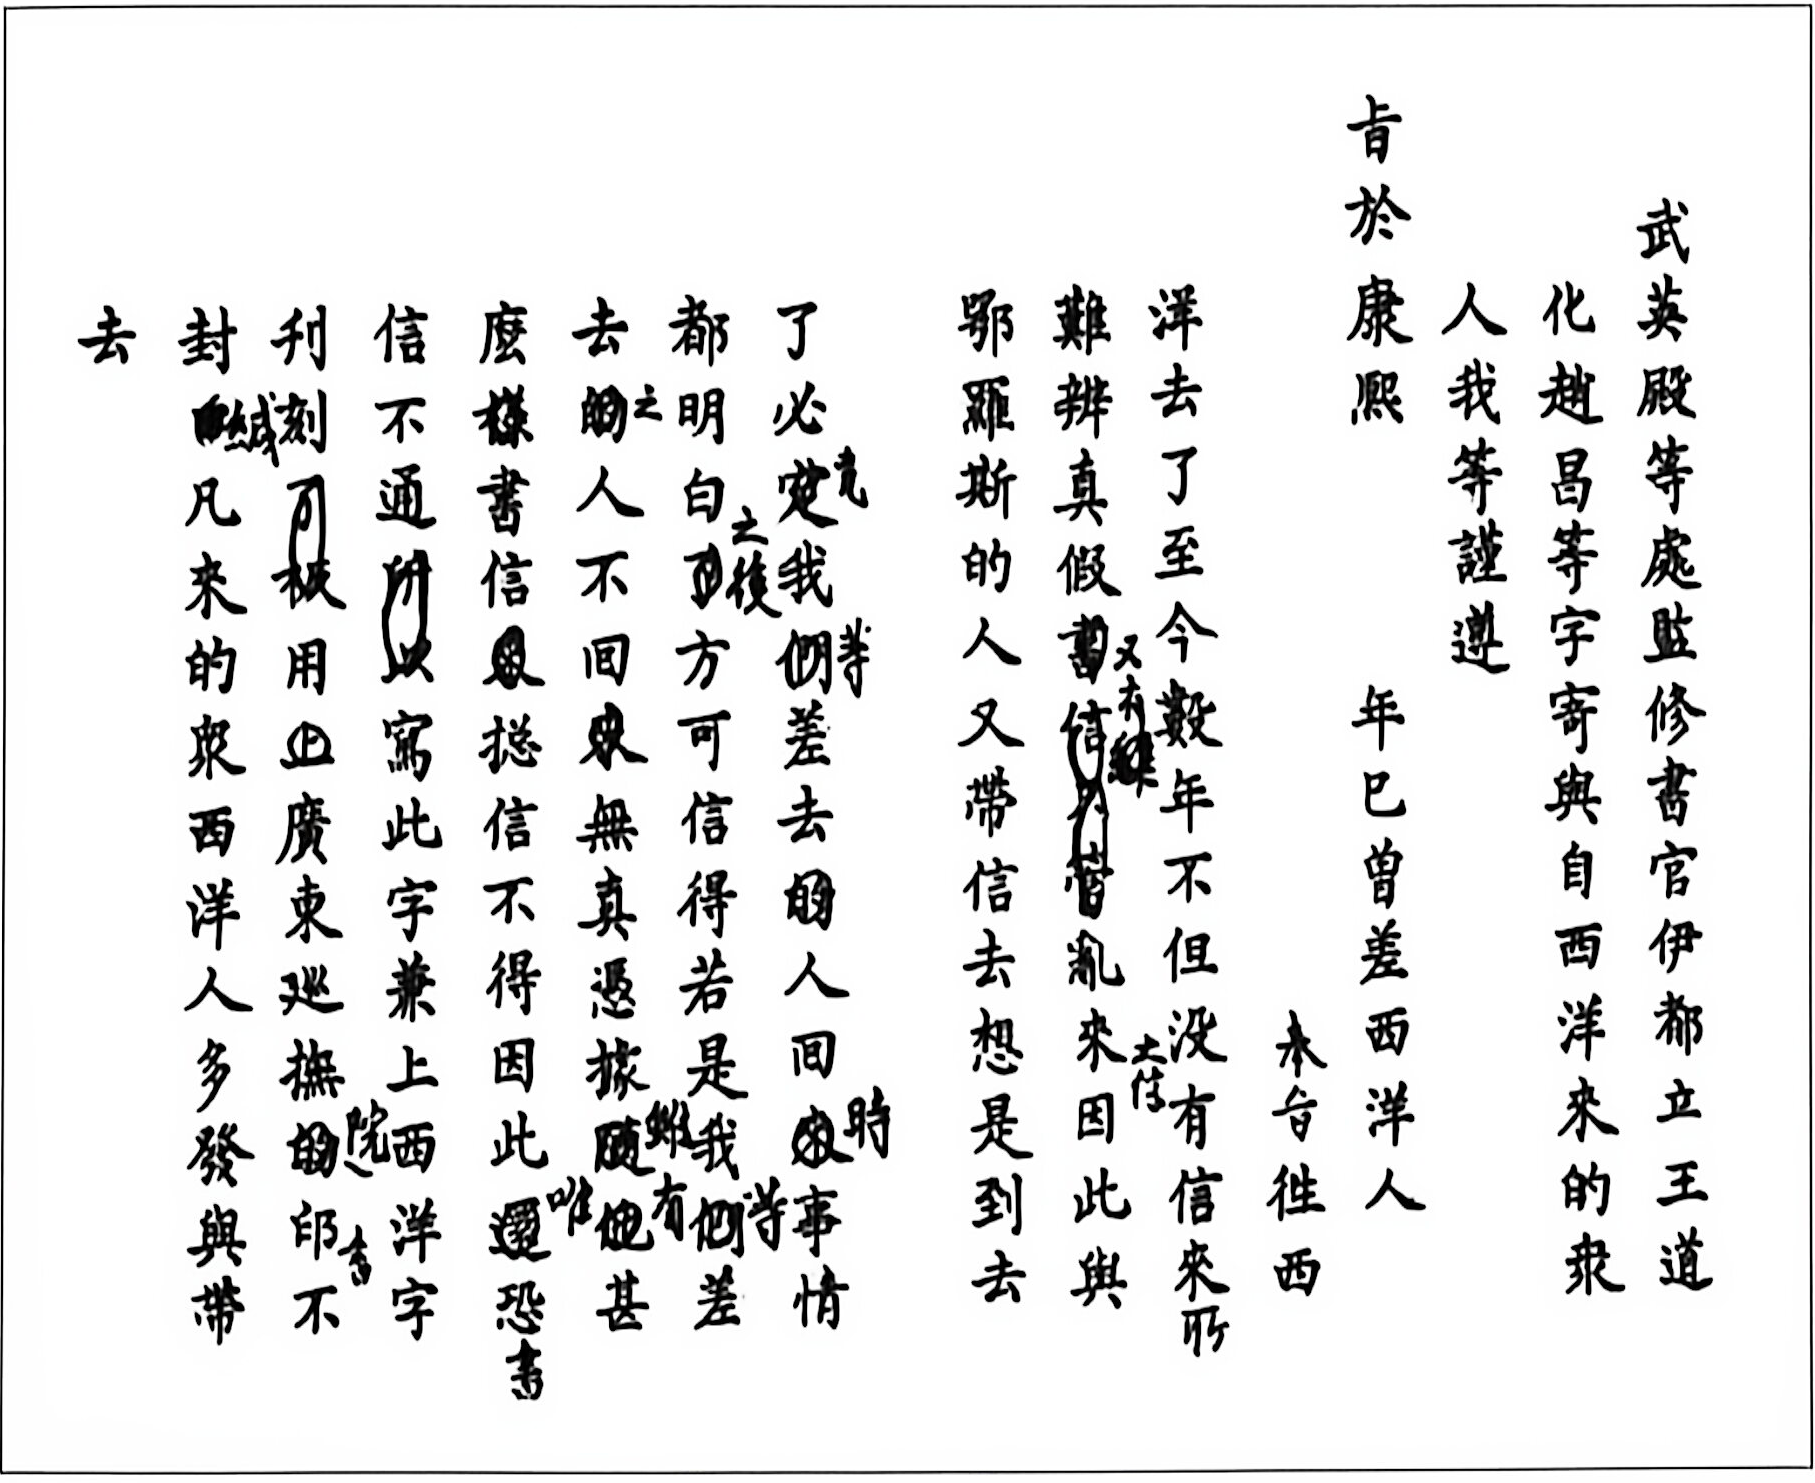
\includegraphics[width=\linewidth,height=.76\textheight,keepaspectratio]{assets/figures/kangxi-red-ticket-draft.png}
\caption*{图0.1\quad 康熙御批红票草稿}
\BookFloatNotes{图片来源：陈垣编，《康熙与罗马使节关系文书》，文件9。}
\end{figure}%
瑟四位西洋人都是来华的传教士，清代官修史书中并没有提到过这%
四人出使西方，他们到底是以什么身份被康熙派出的？红票中只说%
四人是被“差”去西洋，是“奉旨往西洋去了”。同时，红票中的拉%
丁文翻译，写的也是被皇帝派往欧洲，没有给出一个名号。龙安国%
原名 Antonio de Barros，是葡萄牙人；薄贤士原名 Antoine de Beauvol-%
lier，是法国人。二人去欧洲时选择跨越太平洋，走的是美洲路线，到%
达巴西后还给欧洲寄过信，但后来二人在从巴西去欧洲的路上遇到%
风暴，死在了途中。艾若瑟原名 Giuseppe Provana，是意大利人；陆%
若瑟原名 José Raimundo de Arxo，是西班牙人。这二人走的是印度洋%
路线，最后都到达欧洲，还受到了葡萄牙国王的热情接待。陆若瑟%
到达欧洲不久后就病故了。在红票传到欧洲时，只有艾若瑟还活着。%
教皇看到红票以后，批准艾若瑟返回中国。可惜艾若瑟在回程的船%
上去世了。艾若瑟离开中国的时候，还带了一个中国弟子，叫樊守%
义。他一直跟着艾若瑟在欧洲游历，最后守着艾若瑟的棺材抵达广%
州。康熙后来派人去广州，买了36亩土地用作墓地，风光厚葬了艾%
若瑟。当然这段厚葬的历史，清史中也没有记载。艾若瑟的墓早已%
被毁，现在只有一些大理石墓碑残片，存于广州市博物馆中。好在%
19世纪后期，艾若瑟的墓地是当时洋人爱去的一个景点，一位行经%
此处的英国人在游记中详细记录了墓地的情况，还把当时墓碑和墓%
志铭上的拉丁文和汉文全部抄录了下来。在这份抄录中，我们可以%
看到艾若瑟的墓碑正面，刻出的是“钦差艾公之墓”，也就是说康熙%
赐给艾若瑟的名头是“钦差”。艾若瑟的墓碑上还有长篇墓志铭，记%
录下了康熙派内务府人到广州操办墓地的事，同时还比照《汉书·苏%
武传》，赞美了艾若瑟“钦差大西洋公干”而滞留海外十三载后，不%
虑“波涛险幻，坚为复命”的美事。盖棺而后论定，这四位来华的%
欧洲传教士在康熙心中，都是他的“钦差”。%
\par
% 原书页码：vii–viii；段落（跨页续段）
为什么大清皇帝会派洋人做自己的“钦差”出访？这些传教士和%
康熙是什么关系？他们为什么能得到康熙的信任？这些都是本书要探%
索的问题。红票的拉丁文下面，还有十六位来自欧洲各国的在京传教%
士，为康熙发出的红票签名，确认红票内容的真实性。%
% 原书页码：vii；图表（图题／表题所在页）
% 原书页码：vii；表格、表题与表注共用一个环境。
\begin{table}[!htbp]\phantomsection\label{table-16}
\centering\BookTableStyle
\begin{tabularx}{\linewidth}{|>{\raggedright\arraybackslash}X|>{\centering\arraybackslash}p{18mm}|>{\centering\arraybackslash}p{20mm}|>{\centering\arraybackslash}p{18mm}|}
\hline
英文拼写 & 中文名 & 入华时间 & 国家 \\ \hline
Matteo Ripa & 马国贤 & 1710 & 意大利 \\ \hline
Teodorico Pedrini & 德里格 & 1711 & 意大利 \\ \hline
Kilian Stumpf S. J. & 纪理安 & 1694 & 德国 \\ \hline
Joseph Suarez S. J. & 苏霖 & 1684 & 葡萄牙 \\ \hline
Joachim Bouvet S. J. & 白晋 & 1687 & 法国 \\ \hline
Jean-François Foucquet S. J. & 傅圣泽 & 1699 & 法国 \\ \hline
Dominique Parrenin S. J. & 巴多明 & 1698 & 法国 \\ \hline
Pierre Vincent de Tartre S. J. & 汤尚贤 & 1701 & 法国 \\ \hline
Pierre Jartoux S. J. & 杜德美 & 1701 & 法国 \\ \hline
Jean Francisco Cardoso S. J. & 麦大成 & 1710 & 葡萄牙 \\ \hline
Joannes Mourao S. J. & 穆经远 & 1710 & 葡萄牙 \\ \hline
Giuseppe Baudino S. J. & 鲍仲义 & 1694 & 意大利 \\ \hline
Frantz Stadlin S. J. & 林济各 & 1707 & 瑞士 \\ \hline
Jacobus Brocard S. J. & 陆伯嘉 & 1701 & 法国 \\ \hline
Joseph da Costa S. J. & 罗怀忠 & 1715 & 意大利 \\ \hline
Joseph Castiglione S. J. & 郎世宁 & 1715 & 意大利 \\ \hline
\end{tabularx}
\end{table}%
%
这些签名的传教士和康熙又是什么关系？康熙和传教士关系密切并不%
是什么秘闻，当年传教士在寄回欧洲的信中经常炫耀他们和康熙的关%
系，以至于有些欧洲人燃起了一丝希望：康熙有没有可能成为第二个%
君士坦丁大帝（罗马第一个接受基督教的皇帝）？%
\par
% 原书页码：viii；段落
从中国的政治史角度看，康熙和传教士的关系也很特殊。大部分%
传教士都没有官衔，却能往来于宫中，侍奉在康熙左右。紫禁城按功%
能分为内廷和外廷。大臣上朝议事，处理公务都在外廷；内廷算是皇%
帝的私人领域，是皇帝生活起居与日常办公的地方。让当时朝臣都羡%
慕的是，传教士被康熙允许出人内廷。尽管有几个传教士在朝廷也有%
过官衔，负责天象观测这种技术活儿，但按理他们都是不能出人内廷%
的。出入紫禁城从来不是件容易的事，更不要说日常出现在皇帝身边。%
以前的研究者大多都认为，传教士能在康熙左右，是因为康熙对西学%
感兴趣，传教士对他有用处。这种说法颠倒了先后关系。兴趣源自接%
触，康熙对西方学问的兴趣，是不可能凭空产生的。古往今来，能长%
时间接触到皇帝，先决条件都是信任。所以先后顺序应该是，康熙先%
有了对传教士的信任，才会有和他们的接触，从而他们才有机会教康%
熙西方的学术和技术。只有康熙学习了这些知识以后，他才能对西学%
有兴趣，也才能理解传教士那些学问的用处所在。%
\par
% 原书页码：viii–ix；段落（跨页续段）
康熙对传教士的信任，不仅仅体现在让他们出入紫禁城，派他们%
去欧洲，甚至连跟俄罗斯的边界谈判这样核心的国家事务，他也派出%
了两位传教士加人到谈判队伍中。著名的1689年中俄《尼布楚条约》，%
就是两位传教士作为清朝的实际谈判代表，和俄罗斯人谈出来的。双%
方会谈语言是拉丁语。最后的合约由拉丁文、满文和俄文三种语言签%
订，没有汉文。传教士在谈判中说着拉丁文但又忠于清朝，这让俄罗%
斯谈判代表很吃惊，而且他们发现传教士坚决捍卫清朝利益，比以前%
谈判过的满人还要强硬。最后签订的条约，彼得大帝不满意，而且对%
传教士竟然帮助异教徒谈判很不理解，一怒之下，把两位传教士所属%
的耶稣会给禁了，不允许任何耶稣会的传教士进入俄罗斯。%
\par
% 原书页码：ix；段落
在北京的传教士，大多都属于耶稣会。耶稣会1540年成立于欧%
洲。在环球航海的大背景下，耶稣会立会的一个宗旨就是要把天主%
教传播到世界各地，这一点得到了罗马教皇的支持。该会七大创始人%
之一圣方济各·沙勿略（St. Francis Xavier）早在 1551年就远渡重洋，%
来到了广东外面的岛屿，准备找机会进入中国。后来著名的利玛窦神%
父，也是耶稣会传教士，他是在万历年间进人的中国内陆。之后陆续%
到达的耶稣会神父一直孜孜不倦地探索如何融入中国的士大夫圈子，%
在中国传播他们的福音。耶稣会神父在江南成功进入了一些文人圈%
子，同时也为一些当时的名人施洗人教。明朝末年，耶稣会神父汤若%
望进入了朝廷体制，在明朝的钦天监做官。当时他在京城与朝野士人%
多有结交。%
\par
% 原书页码：ix–x；段落（跨页续段）
明清易代之际，在华传教士跟当时所有国人一样经历了战争的痛%
苦。对他们来说，朝代更替也是一次机会，一个让他们走进统治阶层%
权力圈子的机会。传教士从最初见到进京的多尔衮，到后来的顺治皇%
帝，再经历鳌拜专权，最后走进康熙的世界。在康熙的孩提时代，传%
教士就在他身边。在康熙跟着翰林们学习汉语和经史子集的同时，传%
教士在内廷里教他数学等西方学问。传教士后来又一步步地帮助康熙%
和欧洲建立起了各种联系，同时也让欧洲对这个东方皇帝产生了兴趣。%
莱布尼茨、伏尔泰等欧洲科学家和哲学家都在饶有兴致地阅读康熙的%
传记。红票正好是全球化之初中西交流中留下的一页。大概也是近年%
中外历史学界对这段历史的挖掘，让红票的历史位置日渐清晰，拍卖%
中的红票，一路竞价，最后以161万成交。%
% 原书页码：无印刷页码；卷首插图，图1原件漏扫，其完整图注见扫描020。
% 用户于2026-10-12确认缺图为康熙坐像。以故宫藏《康熙帝读书像》高清公开图补入。
% 图像来源：https://commons.wikimedia.org/wiki/File:康熙帝读书像轴.jpg
% 馆藏说明：https://www.dpm.org.cn/collection/paint/230329.html
\par
\begin{figure}[p]\phantomsection\label{fig-front-kangxi}
\centering
% 原文件保持完整；排版时仅裁去右侧拍摄色卡边缘（70像素）。
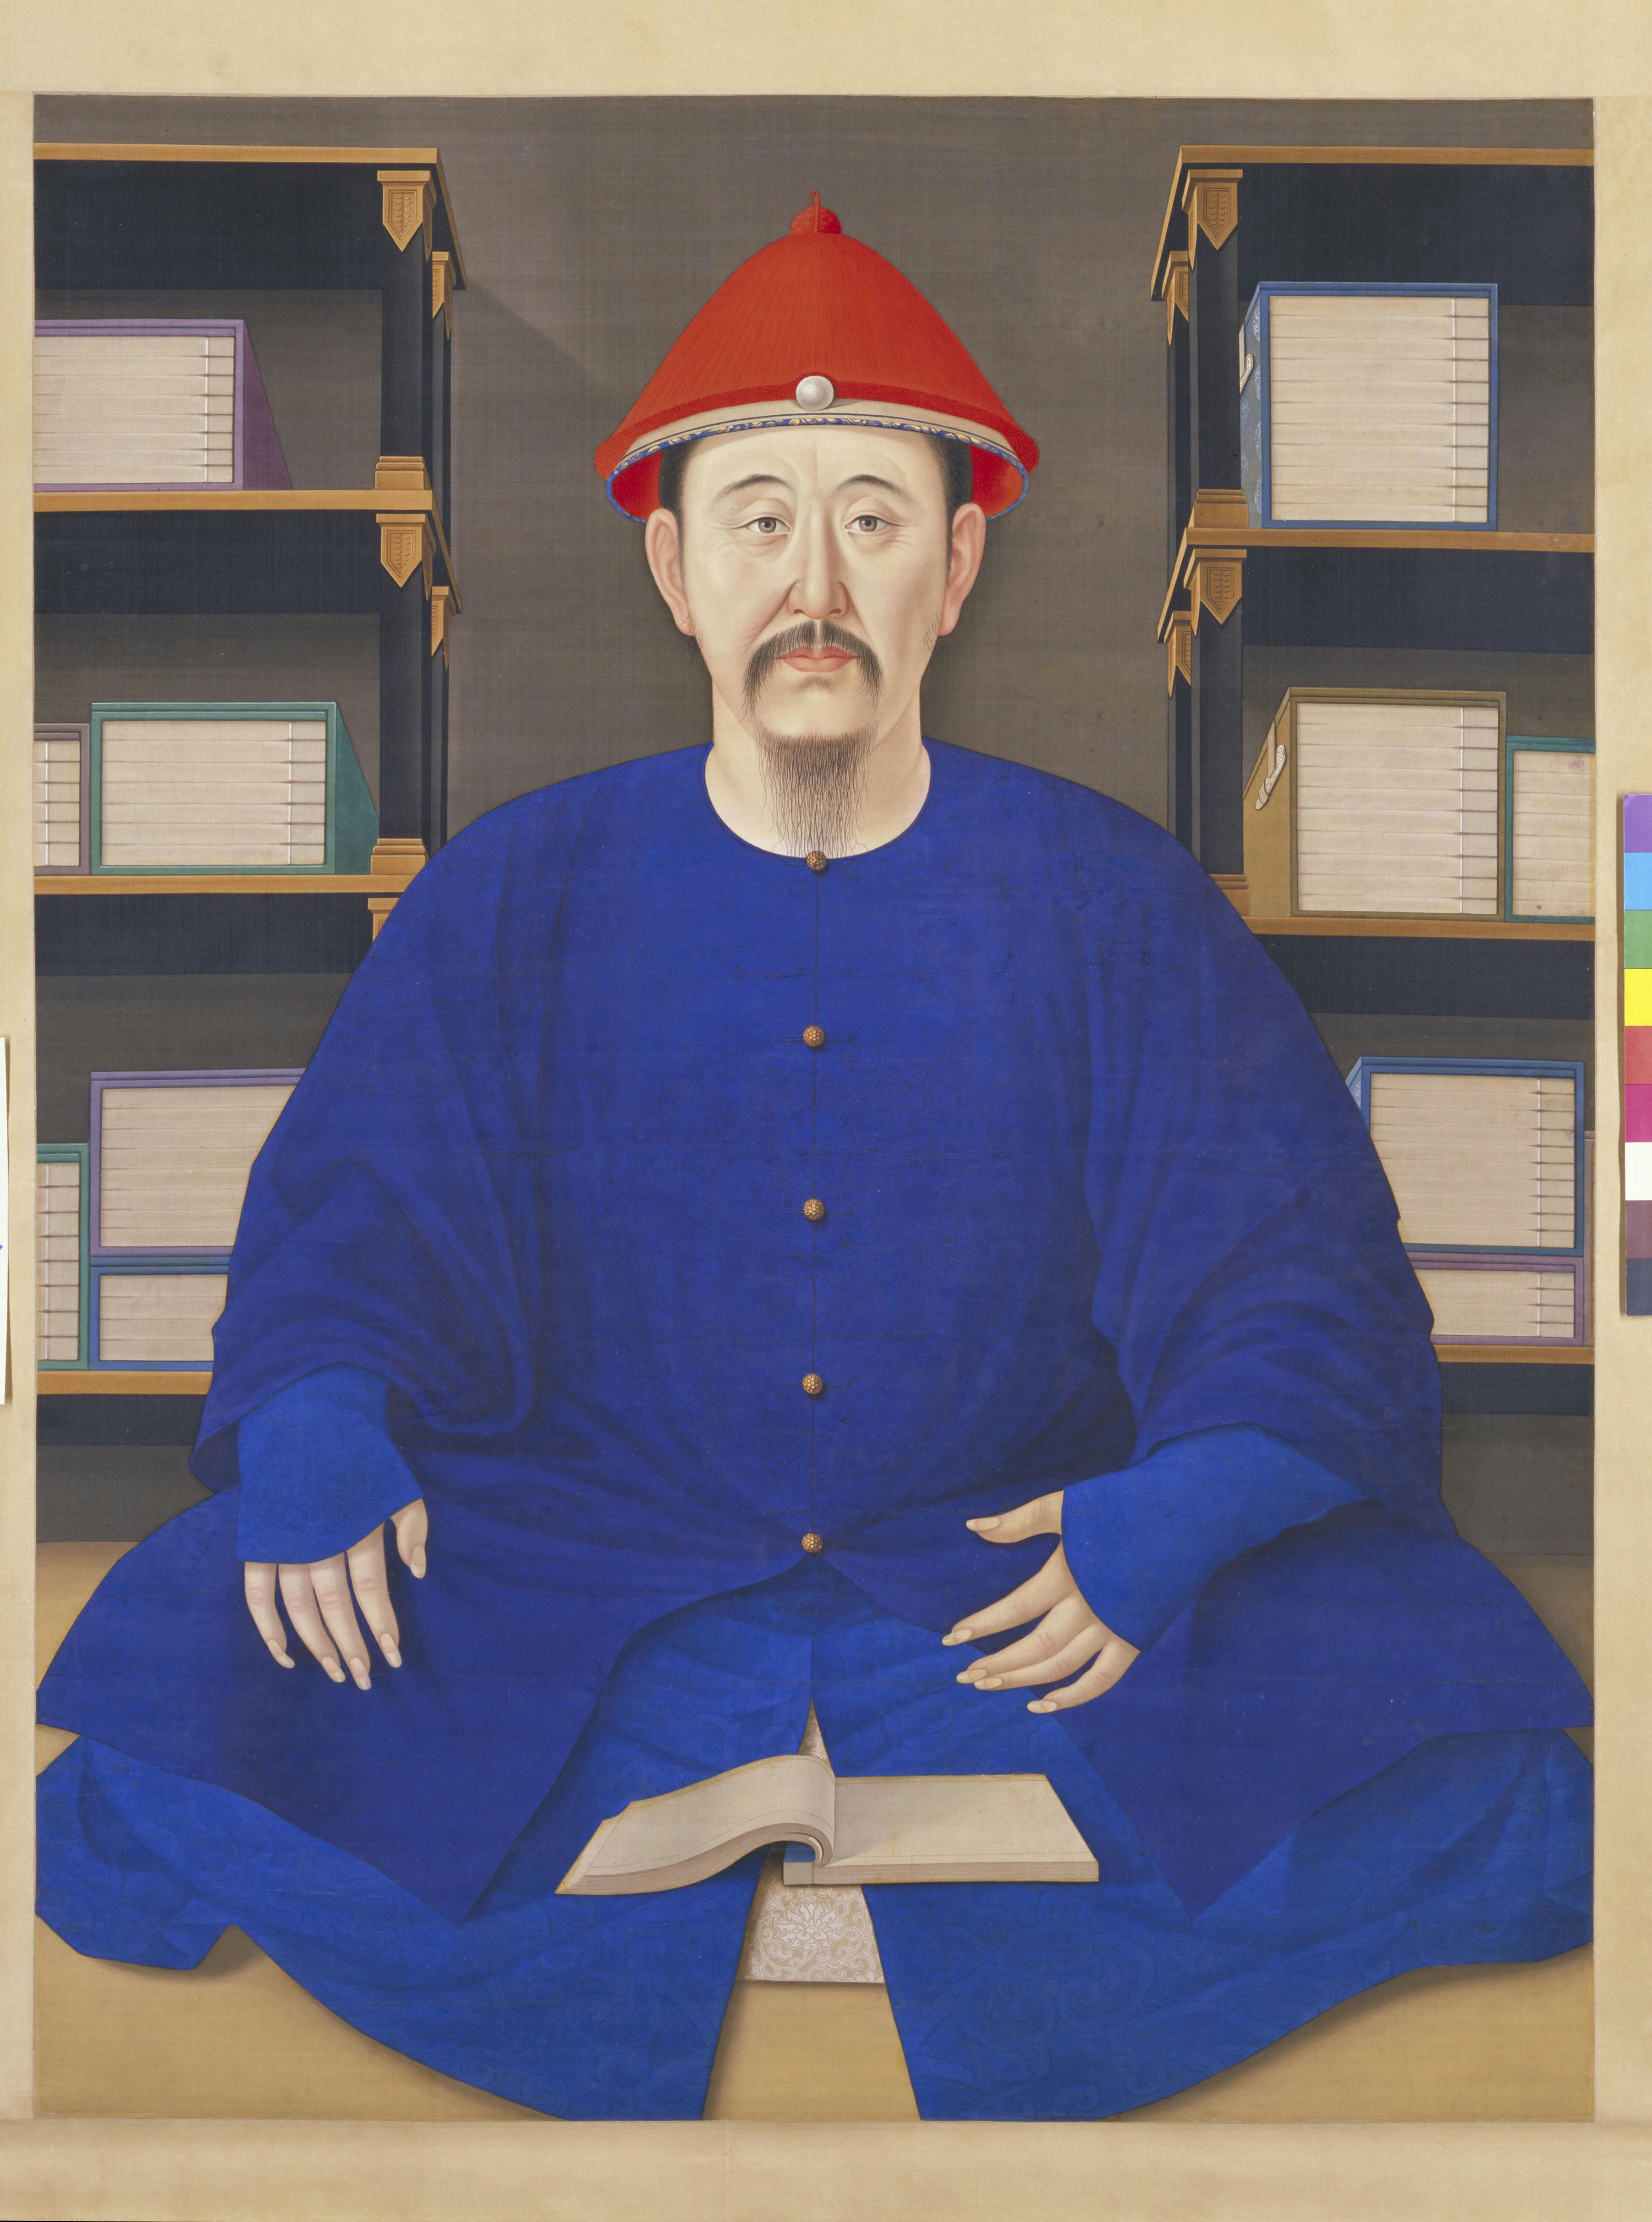
\includegraphics[width=\linewidth,height=.76\textheight,keepaspectratio,trim=0 0 70bp 0,clip]{assets/figures/kangxi-reading.jpg}
\caption*{图1\quad 康熙坐像，故宫博物院藏。画中人物和书架的透视关系以及后面的阴影都是典型的西洋画技法，展现出全球化之初中西文化的互动。}
\end{figure}%
% 原书页码：无印刷页码；卷首图2与图注见扫描020。
\begin{figure}[p]\phantomsection\label{fig-front-tapestry}
\centering
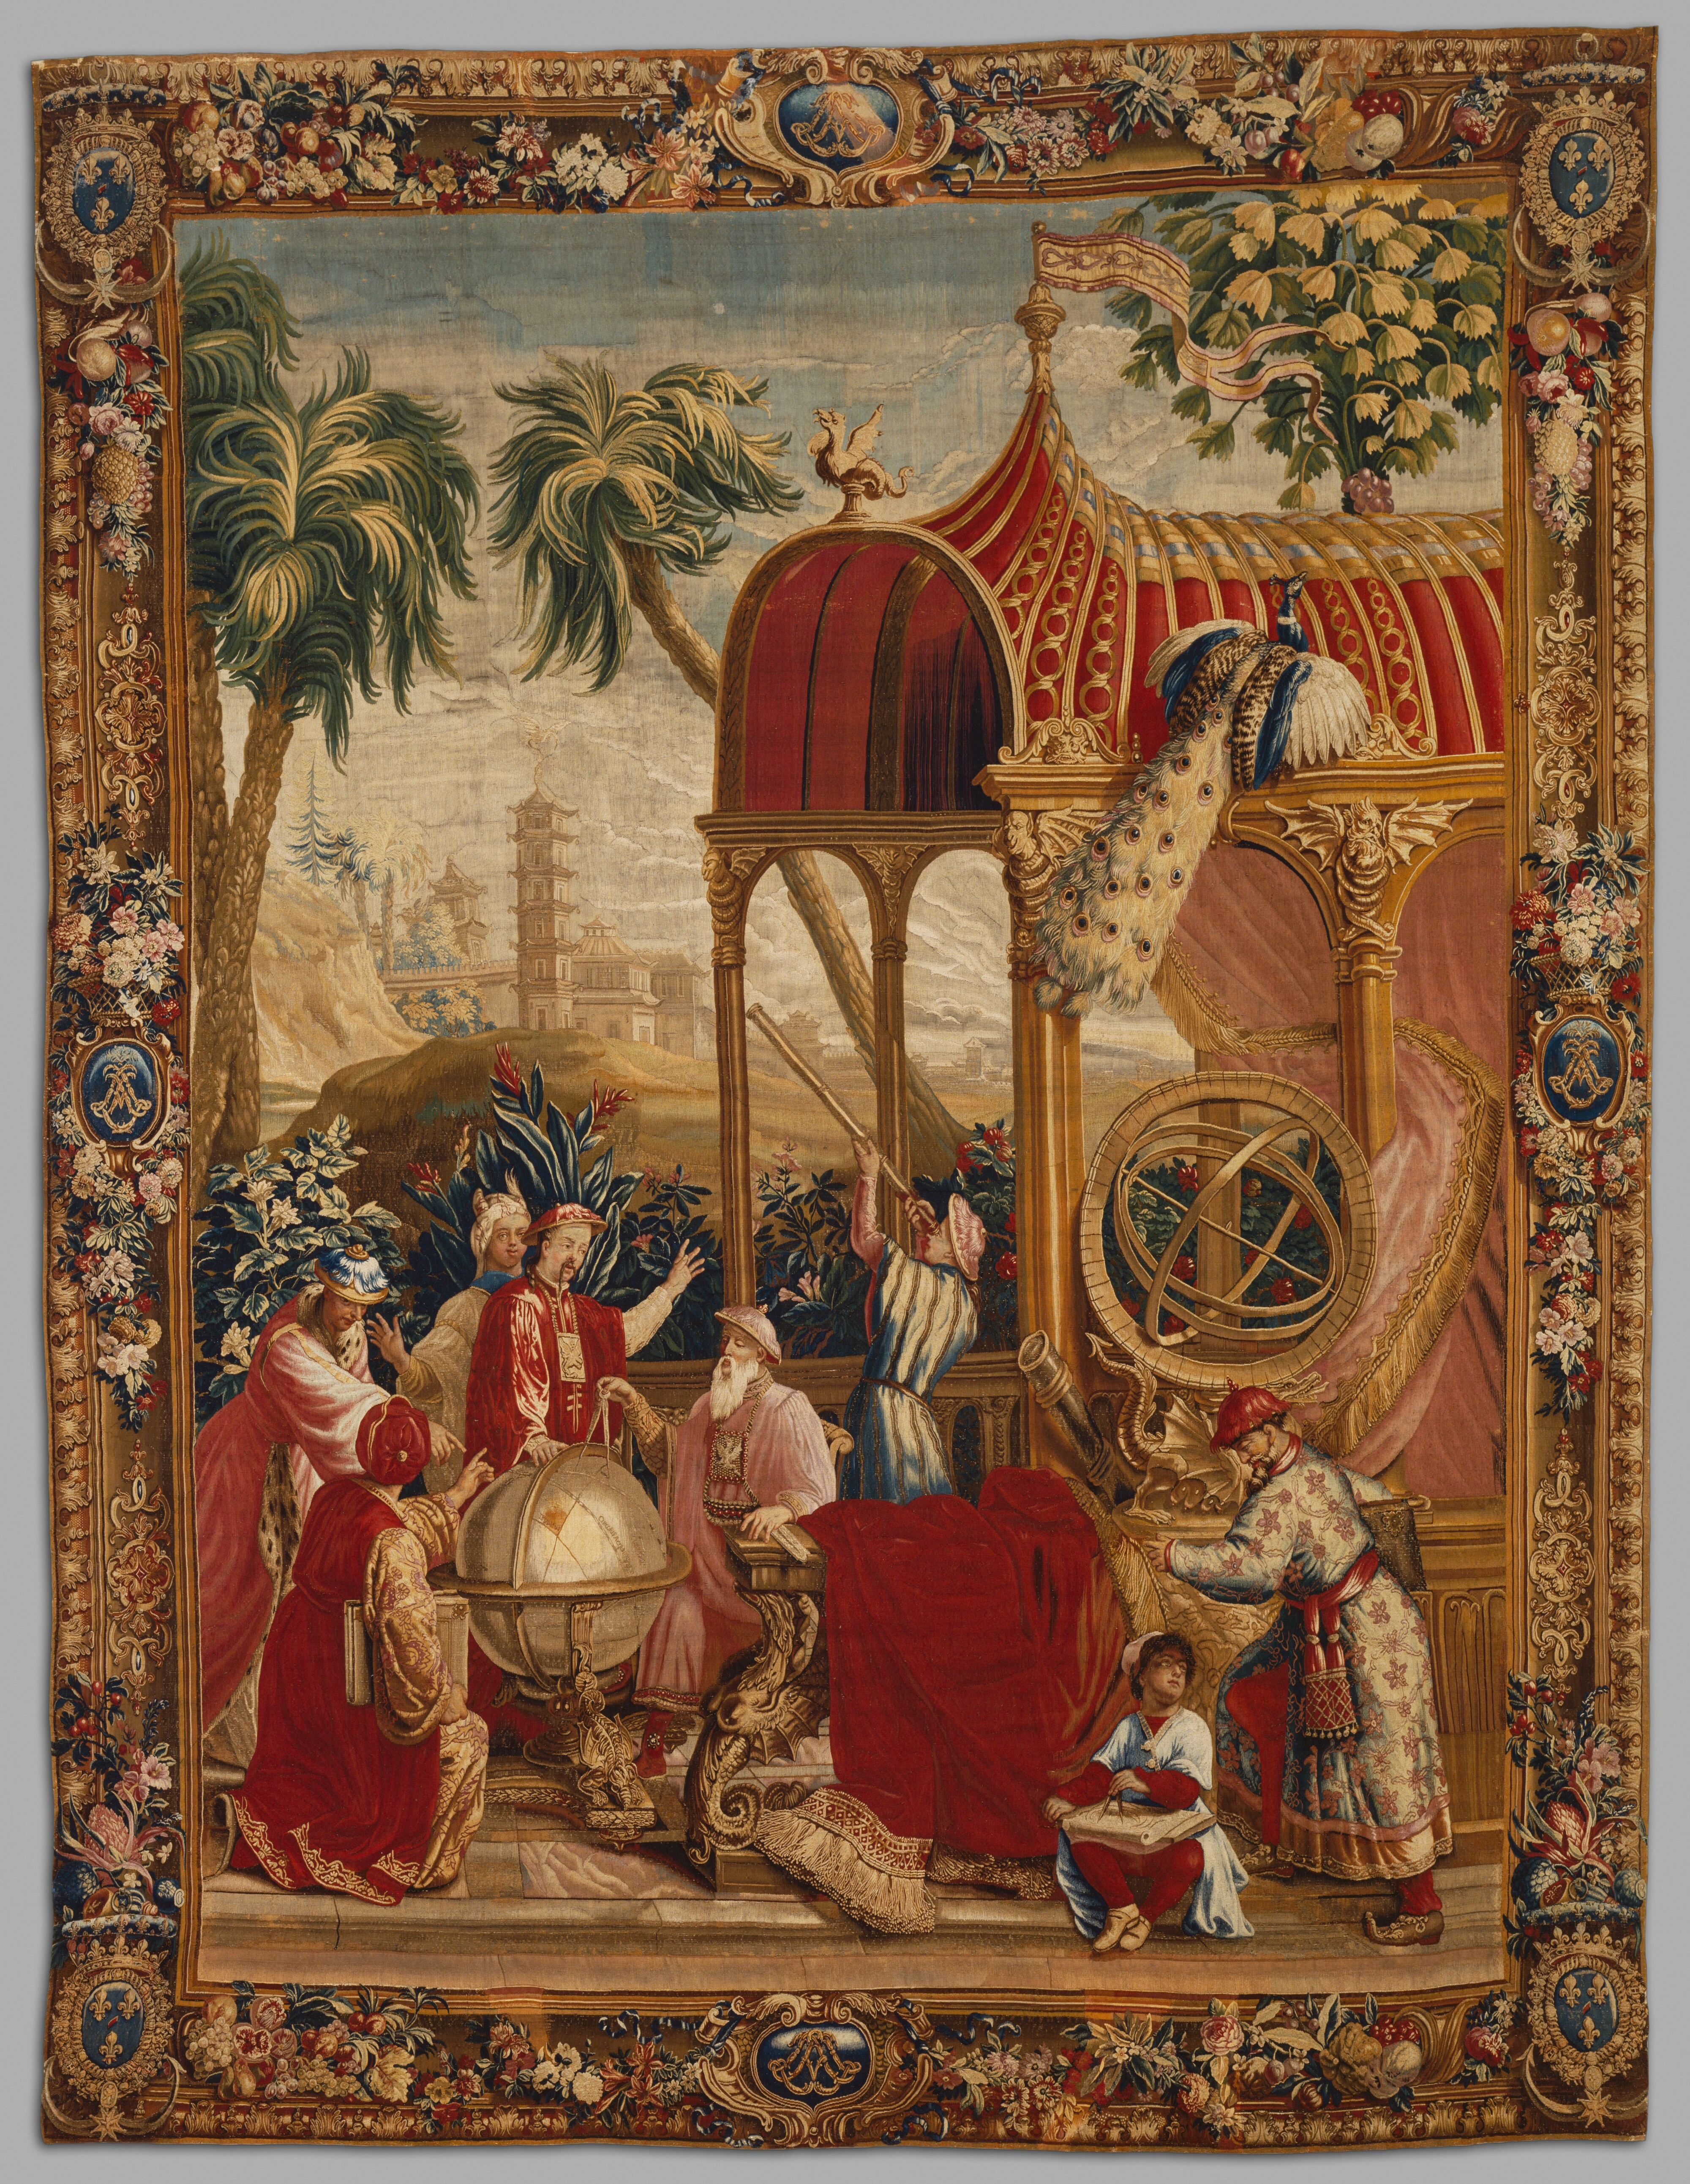
\includegraphics[width=\linewidth,height=.76\textheight,keepaspectratio]{assets/figures/emperor-tapestry.jpg}
\caption*{图2\quad “中国皇帝外出巡幸”挂毯。尺寸：254×415.3cm，产地：法国，年份：1697—1705。盖蒂博物馆藏。挂毯图案为根据入华传教士写回欧洲的信件中关于中国皇帝的故事而想象创作。}
\end{figure}%

\clearpage\markboth{第一部分\quad 进入清朝权贵圈的西洋人}{第一部分\quad 进入清朝权贵圈的西洋人}
% 第一部分 进入清朝权贵圈的西洋人
% 原书页码：无印刷页码；标题
\part{进入清朝权贵圈的西洋人}

\clearpage\markboth{第一章\quad 佟家的奴才}{第一章\quad 佟家的奴才}
% 第一章 佟家的奴才
% 原书页码：003；标题
\section{佟家的奴才}
\par
% 原书页码：003；段落
顺治十二年二月二十七日（1655年4月3日），耶稣会传教士利%
类思和安文思给顺治皇帝呈上六件礼物外加一份中文写的奏本，感谢%
顺治皇帝以及清朝长期以来对他们的优容和恩养。在奏本中，他们简%
要介绍了他们一路走来的经历。奏本是这样写的：%
\par
% 原书页码：003；段落
{\bookkai 大西洋耶稣会士远臣利类思、臣安文思谨奏：}%
\par
% 原书页码：003；段落
{\bookkai 为微臣感恩无地，敬进西国方物，以表臣忱事。臣等产于西洋，}%
{\bookkai 从幼弃家修道。明季东来至蜀，居堂传教，历有年所，不意遭寇掳待}%
{\bookkai 戮。于顺治三年，幸逢大兵西剿，恭遇肃王恩释，依随来京。仰荷皇}%
{\bookkai 上隆恩，特送礼部及光禄寺，图赖固山家豢养，朝夕焚祝万寿，经今}%
{\bookkai 五载，感激无涯。兹有方物六种，躬献阙庭，伏祈皇上，俯赐敕收。\NoteRef{1}{1}}%
\par
% 原书页码：003–004；段落（跨页续段）
两位神父明朝末年就到了中国。利类思是西西里人（现属于意大利），%
1636年（崇祯九年）来华；安文思是葡萄牙人，1642年到成都，和%
利类思一起在那里传教。后来二人一直一起在中国传教，直到安文思%
1677年去世。%
\par
% 原书页码：004；段落
当1655年二人上这份奏本的时候，他们已在中国待了快二十年，%
早已不是来华的新人了。奏本中的遣词造句也可以看出，二人对于清%
初官场政治很了解。奏本感谢了肃王豪格和佟图赖固山（固山是八旗%
内的官职，是一旗的统帅，后改为都统）两个人，然后还提到了两个%
机构：礼部和光禄寺。为什么会感谢人的同时，又感谢机构，而不是%
感谢负责这个机构的人呢？这恰恰显示出了二人的圆滑老练，因为他%
们要隐藏和一个人的关系。%
\par
% 原书页码：004；段落
这个人就是摄政王多尔衮（1612—1650）。当二人在1648年跟着%
豪格的征西大军班师归来抵京时，他们的身份有两个：一是叛贼张献%
忠朝廷的逆臣；二是战地俘虏，已归为奴籍。\NoteRef{1}{2}所以二人到京之时，是%
戴罪之身。当时在京做官的同为耶稣会神父的德国人汤若望，既不敢%
和他们联系也不敢把他们收留在他的教堂中。\NoteRef{1}{3}但当时实际掌控北京%
的多尔衮，并没有为难二人，反而把二人交给专管接待外交使节的礼%
部来照顾，并且还给予了他们在北京城中活动的自由。\NoteRef{1}{4}对于在成都%
张献忠的大西朝当过官的人来说，这二人最初能在北京没有被追究，%
并平稳地安顿下来，不得不说多尔衮对二人是有恩的。但是，二人上%
奏本的时候，多尔衮已经去世五年，早已不是一个可以在朝堂上提及%
的人。多尔衮的爵位在他死后几个月，就因为朝堂政治斗争被剥夺了。\NoteRef{1}{5}%
两个神父很清楚当时的政治气氛，知道哪些名字可以提，哪些不能提。%
\par
% 原书页码：004–005；段落（跨页续段）
当然，他们提到的两个人，豪格和佟图赖，都是当时政治气氛中%
对于他们有利的人。那两个神父又到底跟这两位满人权贵有什么联%
系？这其实就涉及两位神父是如何从张献忠朝廷的罪臣身份一步步和%
满人权贵搭上线的问题。从二人1648年进京算起，到1677年安文思%
去世、1682年利类思去世，他们在满人统治下的北京待了超过三十年，%
历经了两位清朝皇帝。要了解二人怎么慢慢进人满人朝廷的故事，就%
得从他们与两位满人权贵的关系说起。%
% 原书页码：005；标题
\subsection{战场上的俘虏}
\par
% 原书页码：005；段落
跟二位神父相关的大清历史大概得追溯到1643年，也即满人人关%
的前一年。后世称为清太宗文皇帝的皇太极（1592—1643），在没有%
留下遗诏指定继承人的情况下，这一年突然驾崩了。这不可避免地引%
发了各方势力的争位行动。简单来说，当时有两方势力不分伯仲，一%
派支持皇太极的长子豪格继位，另一派支持皇太极的弟弟多尔衮。为%
了避免满人内部的分裂，双方妥协达成了第三个方案：推举皇太极的%
第九子、当时六岁的福临，也就是后来的顺治皇帝登位。作为附加条%
件，多尔衮和济尔哈朗（努尔哈赤之侄）一起为顺治当摄政王。虽然%
最后皇位问题得以妥协解决，但是争位的多尔衮和豪格叔侄双方成了%
仇敌。%
\par
% 原书页码：005–006；段落（跨页续段）
1648年3月，也就是满人控制北京的第四年，多尔衮以谋反的罪%
名逮捕了豪格。逮捕前一个月，豪格刚结束四川西征，剿灭了张献忠，%
得胜回京。豪格在被逮捕当月就死于狱中。无论正史、野史都基本一%
致认为豪格是被多尔衮害死的。最让时人惊诧的是，多尔衮在豪格死%
后，还把豪格的夫人纳人府中。就连北京的汤若望神父也把这当成奇%
谈写进了他发回欧洲的信中。%
\par
% 原书页码：006；段落
1650年12月，多尔衮去世。在他死后两个月，顺治皇帝就在济%
尔哈朗的支持下剥夺了多尔衮家的爵位，瓦解了多尔衮在朝廷中的残%
余势力。同时，豪格的所有爵位得到了恢复。1651年以后，多尔衮就%
不是适合在朝堂上攀附的名字了。%
\par
% 原书页码：006；段落
有了这个背景，才可以理解为什么两位神父在奏本中提到了豪格，%
而不提多尔衮。不过，两位神父提豪格也不能算是攀附。因为二人确%
实和豪格有实在的联系。豪格是西征张献忠大军的最高统帅，而两位%
神父于1644至1647三年间在张献忠成都的朝廷中做官。\NoteRef{1}{6}按他们自己%
的话说，他们是张献忠大军进人成都后，为了活命不得不听命于张献%
忠。他们从西医角度，认为张献忠患有精神疾病，也亲眼见证了张献%
忠残酷掠杀老百姓。后世各种关于张献忠暴虐的传闻，都能在二人的%
记录中得到印证。%
\par
% 原书页码：006；段落
两位神父是在战场上遭遇豪格大军的，两人都在战场上中箭倒地。%
他们的欧洲人面孔救了他们，赶上来补刀的满人士兵没有杀他们，反%
而把他们带到豪格的大帐中。所幸当时随军的满汉语翻译和北京的汤%
若望神父有私交，救了二人的命。有了随军翻译的这层关系，二人虽%
然是战俘，并没有被为难，还得到了特别的关照。\NoteRef{1}{7}%
\par
% 原书页码：006–007；段落（跨页续段）
从四川被俘到最后1648年落脚北京，二人在豪格部队中跟着满%
人士兵一起走了一年半左右。\NoteRef{1}{8}很多满人士兵也知道二人，知道豪格%
关照他们。有一次，豪格传令大部队，让士兵在各自俘虏中寻找两位%
神父的一个仆人。最初，抓住这个仆人的满人士兵并不想把他交出来，%
后来听说是豪格在找这个人，这个士兵亲自把仆人带到豪格帐内，当%
成礼物送给了豪格。\NoteRef{1}{9}%
\par
% 原书页码：007；段落
满人传统中，士兵行军打仗都是自备武器和粮草，擒获的战俘归%
士兵私有，成为士兵的奴隶。对于士兵来说，获得战利品和获取奴隶%
都是同等重要的经济回报。在满人世界中，奴隶和牛、马、衣服这些%
一样，都是私有财产。奴隶最大的来源就是战场上的俘虏，所以俘获%
仆人的士兵一开始并不想交人；后来他把仆人交给豪格，和献给豪格%
一匹布是差不多的。%
\par
% 原书页码：007；段落
由于有豪格的照顾，满人士兵不久也把两个神父当成了自己人。%
大概在二人被俘五个月以后，部队回京路过西安。这时，两个神父已%
经知道满人军队内部的行事习俗。当时满人军队进人城市，按例都要%
临时征用寺庙等公共设施来驻扎。两位神父率先找到了当地的天主教%
堂，住进去后，就对后来的士兵吹嘘这里已经被部队内某某大人物征%
用了。士兵听他们这样说，就离开另寻他处去了。\NoteRef{1}{10}%
\par
% 原书页码：007–008；段落（跨页续段）
当然，两位神父跟着满人部队，适应满人生活的过程还是很痛苦%
的。从他们第一天在战场遇到满人士兵，他们就知道这些士兵是“外%
国人”。这些人和他们熟悉的汉人不一样，不会说汉语。尽管二位神%
父早已精通汉语，无奈从士兵到豪格，都不通汉语，完全没办法交流，%
他们所有交流都需要翻译。\NoteRef{1}{11}1满人军人吃的也和汉人不一样，两位神%
父得跟着满人学他们在行军中吃马肉。\NoteRef{1}{12}跟着满人军队以后，两位神%
父的基本身份也跟以前在明朝以及在张献忠大西朝廷的不一样了，因%
为现在他们不算皇帝的臣民，而就是擒获他们的人的奴隶，是他们主%
子的私有财产。最开始的时候，两位神父各自有自己的主子。这样他%
们二人的生活，比如吃什么，吃多少，都由二人的主子决定。利类思%
运气较好，他的主子比较大方，能基本吃饱。但安文思就没有那么好%
运气，他的主子连基本食物都不给够，他好几次都差点饿死在路上。\NoteRef{1}{13}%
\par
% 原书页码：008；段落
在行军路上的某个时候（1647—1648），二位神父的奴籍被转到了%
豪格名下。主奴关系是满人八旗世界中最基本的阶层关系之一。在满%
人的理念中，主子给奴才提供生活所需，而奴才对主子尽忠。\NoteRef{1}{14}满人%
统治者也深知奴隶是重要的经济资源。因而他们推崇主奴之间以家为%
单位，和睦相处。用努尔哈赤的话说，就是要形成一种“奴才爱主子，%
主子爱奴才”的社会。\NoteRef{1}{15}由于主奴关系中蕴含着家庭关系，因而外人%
在对待一个奴才的时候得看主人是谁；同样，要是主人升官了，自家%
奴才也跟着高兴，感觉脸上有光。%
\par
% 原书页码：008；段落
满人人关以后，汉族大臣极力反对满人的主奴统治，但满人上层%
还是力排众议，坚持主奴关系是满人八旗制度的基础。最有名的例子%
就是清初严厉执行《逃人法》，这个法令的核心就是重罚那些胆敢容%
留逃跑奴隶的人。\NoteRef{1}{16}也是因为这个原因，当汤若望神父知道两位神父%
是奴隶身份，就不敢在他设在北京的教堂中收留他们了。\NoteRef{1}{17}%
\par
% 原书页码：008–009；段落（跨页续段）
对于做过豪格奴才的这一身份，两位神父并没有隐瞒。因为满人%
社会中的奴才和汉人社会的“奴”是不一样的。汉人的“奴”属于贱%
民阶层，地位在贵族、官吏、平民之下。简单来说，在汉人社会，“奴”%
和其他属于贱民阶层的人社会地位低，在社会多方面受歧视，而且%
法律和社会习俗还对贱民阶层有很多专门的行为约束。\NoteRef{1}{18}但在满人社%
会，奴才的身份不代表一个人的社会地位，他们的社会地位主要取%
决于他们主子的社会地位。用通俗的话来说，在满人世界，重要的不%
是你是否是奴才身份，而是做的是谁家的奴才。如果是皇帝和达官贵%
人家的奴才，那是一种有利的身份。%
\par
% 原书页码：009；段落
两位传教士知道做过豪格奴才，表明了他们算是豪格一脉的人。%
这个背景对二人在顺治朝廷是有利的，因而他们在给顺治上奏本的时%
候专门提到这个已经过世了七年的前主子。%
% 原书页码：009；标题
\subsection{康熙母亲的娘家}
\par
% 原书页码：009；段落
在豪格1648年去世以后，两位神父的奴籍转到了佟图赖名下。\NoteRef{1}{19}%
佟图赖是正蓝旗汉军都统，是整个佟氏家族的核心人物。八旗每一旗%
有一位旗主，旗下又分为满、蒙、汉三旗，也就有三位都统。由于旗%
主必须是努尔哈赤家族的后代，所以都统这个职位是非努尔哈赤后代%
在八旗中能达到的最高职位。%
\par
% 原书页码：009；段落
明末以来，佟氏家族一直是满人龙兴之地——辽东地区的名门望%
族。努尔哈赤娶的第一位夫人就来自佟家，他还用“佟”作为他的汉%
族姓氏。佟氏家族从努尔哈赤时期起就在满人政坛中有重要地位。满%
人1644年人关以后，佟家子弟遍布朝野，当时甚至有“佟半朝”一说。%
\par
% 原书页码：009–010；段落（跨页续段）
在满人政坛中，佟氏家族的最大特点是其成员兼具满人和汉人两%
方面的文化特点。由于康熙的母亲出自佟家，因而佟家是汉人还是满%
人就决定了康熙到底有没有汉人血统的问题。历史上一直争论不清到%
底他们是汉化了的满人还是满人化了的汉人。\NoteRef{1}{20}°但无论观点如何，都%
承认佟氏兼具了汉满两方面的特质。在17世纪初，明清在争夺辽东%
的时候，两方也都认为佟氏家族是自己人，两方都在争取他们。\NoteRef{1}{21}在%
辽东地区，佟氏是少有可算作书香门第的家族。1616年，佟卜年中了%
明朝进士。当时明朝廷经营辽东的熊廷弼就把佟卜年招致麾下，希望%
他能作为佟氏的代表，帮自己打理辽东。%
\par
% 原书页码：010；段落
佟氏家族中的佟养性和佟养真在1619年投奔到努尔哈赤帐下。努%
尔哈赤按照游牧民族的老传统，嫁了自己氏族中一位女子给佟养性，%
把他称为额驸（驸马），这样通过婚姻纽带来巩固双方的关系。\NoteRef{1}{22}在明%
廷看来，两位佟氏重要人物投靠努尔哈赤，意味着整个佟氏家族的叛%
变。因而佟氏家族的成员在明朝疆域内集体受到了牵连。按照佟家后%
人的记载，佟家成员一些被迫逃进山区，有些不得不隐姓埋名来躲避%
明廷的追查。\NoteRef{1}{23}佟卜年也被查下狱，最后冤死狱中。至死，佟卜年都%
在喊冤，死前还留下了一份绝笔痛陈其清白。\NoteRef{1}{24}%
\par
% 原书页码：010；段落
满人没有介意佟氏和明朝的种种联系，反而视佟氏家族与汉人的联%
系为佟氏的特有价值所在。努尔哈赤和后来的皇太极都信任佟氏家族的%
人，佟氏家族的人在满人军队和朝廷都得到重用。1620年代以后，皇太极%
更是直接把所有与汉人相关的事务交给佟养性来打理。这包括满人区域%
内的汉人、明疆域内迁徙过来的移民，以及在战争中抓到的汉人俘虏。\NoteRef{1}{25}%
\par
% 原书页码：010；段落
利类思、安文思在奏本中提到的佟图赖是佟养真的二儿子，是满%
人朝廷中“佟二代”的领军人物。从军事上来说，佟图赖声名显赫，%
不仅在最初满人的辽东扩张中有各种军功，在后来攻占明朝本土、消%
灭南明势力时，也立了大功（他带的部队人关以后一直打到广西）。%
人关以后不久，顺治皇帝还娶了佟图赖的女儿。1654年，也就是利%
类思、安文思上奏本的前一年，佟氏给顺治皇帝生了一个儿子。这个%
儿子就是后来的康熙皇帝。%
\par
% 原书页码：011；段落
对于佟氏家族，跟本书相关的一个问题就是，为什么佟图赖会在%
豪格死后，同意接收利类思、安文思成为自家的奴才？而且让他们二%
人吃住在自己的府上，也即让他们做的不是普通奴才，而是包衣奴才？%
“包衣”是满语的音译。据清史前辈孟森解释：“包”是满语“家”的意思，%
而“衣”相当于汉语中的虚字，类似于“之”字。包衣奴才就是指跟主%
子关系最近的、家周围的奴才。\NoteRef{1}{26}满人入关以后，包衣奴才专指满人权%
贵家里面的奴才，是整个奴才群体中地位最高的一群。后来许多清朝%
名人都是包衣奴才出身。比如曹雪芹的祖父曹寅，他就是康熙的包衣。%
\par
% 原书页码：011；段落
对于佟图赖为什么会把两位传教士收入府中做他的包衣，当时在%
北京的汤若望在写给欧洲的书信中解释过，他说是因为佟图赖和西洋%
人的关系一直都好，和他自己的私交也很好。\NoteRef{1}{27}汤若望所谓的“和西%
洋人关系好”指什么？如果真是这样，那么这个好关系又是怎么建立%
起来的？这些问题和佟氏家族及清朝汉军八旗建立的历史有关。%
% 原书页码：011；标题
\subsection{满人对西洋人的印象}
\par
% 原书页码：011–012；段落（跨页续段）
在满人最初辽东发迹的过程中，明军使用的西洋“红衣大炮”一%
直是满人骑兵的心腹大患。当明军在城池上架起西洋大炮，战无不克%
的满人骑兵基本束手无策。17世纪二三十年代，满人军队打的败仗基%
本都和明军用大炮有关。努尔哈赤自己就是在1626年的宁远战役中%
被大炮所伤，几个月后就死了。\NoteRef{1}{28}皇太极在即位后第一年，就兴兵为%
父报仇，但都败在宁远和锦州的大炮之下。不过这也让皇太极认识到%
了大炮的威力，开始致力于发展满人的炮兵部队。在1620年代后期，%
明满双方都意识到了西洋大炮在战争中起到的关键作用。1626年宁远%
大捷以后，明廷甚至派礼部官员给立功的红衣大炮做了祭祀典礼，望%
其能够继续发挥作用，以保大明江山。\NoteRef{1}{29}袁崇焕也在宁远大捷后给朝%
廷奏事时总结道，对付满人最有效的策略就是“凭坚城以用大炮”。\NoteRef{1}{30}%
同样，满人在大凌河之战中使用大炮获得胜利后，也确定行军打仗，%
大炮必不可缺。\NoteRef{1}{31}%
\par
% 原书页码：012–013；段落（跨页续段）
但在1620年代末期，明朝还没有技术仿制欧式的“红衣大炮”，%
而主要依赖从澳门的葡萄牙人那里进口，以及依靠他们训练军队，提%
高大炮的命中精度。1625年，已经受洗成为天主教徒的明朝大臣徐光%
启派了两个门人到澳门去谈购炮之事。当时在澳门的葡商以及传教士%
都认为大炮贸易是天赐良机，可以借此加强和大明的关系。所以澳门%
的商人和传教士对大炮一事都很上心。1629年，耶稣会神父陆若汉%
（João Rodrigues，1561—1634）带领 30 位葡萄牙炮手和 40 尊大炮从%
澳门出发去往北京。\NoteRef{1}{32}1630年1月，队伍在抵达距离北京约60公里%
的小城涿州时，正好遇到了满人南侵围城。他们一行便在城上架起了%
大炮迎敌。据记载，满人骑兵仅仅是听到如雷般的炮声，还没有开始%
真正攻城，就撤退了。\NoteRef{1}{33}有了这个战绩，自然整支队伍到北京后受到%
了相当高的礼遇，而且北京还给团队中每个人开出了很高的薪俸。当%
时只有带队的陆若汉因为自己的神父身份拒绝了明廷的俸禄。明军的%
前线将领得知这批带着大炮的洋人队伍来京以后，都纷纷上书朝廷要%
这些洋人和洋炮。\NoteRef{1}{34}在这一背景下，明廷在5月又派陆若汉带人到澳%
门磋商进一步购买大炮和雇佣葡萄牙炮手的事宜。11月，陆若汉带着%
100名葡萄牙炮手和12门炮从澳门启程赶赴北京。可惜的是，当时明%
廷内部廷议不能平息，一些大臣反对雇佣西洋人。整个队伍到达南昌%
以后，朝廷又命整支队伍返回澳门候旨。\NoteRef{1}{35}%
\par
% 原书页码：013；段落
在满人那边，皇太极命佟养性负责办理所有大炮事宜。1631年2%
月8日，在佟养性监督下，满人制造出了第一批大炮。其中最大的一%
尊取名为“天佑助威大将军”。佟养性的名字连带一帮负责造炮工匠%
的名字都刻在这尊大炮的炮身上。\NoteRef{1}{36}七个月以后，佟养性就用这批大%
炮在大凌河之战中立下了首功。\NoteRef{1}{37}乾隆年间，清朝官修历史总结“红%
衣大炮”的章节，写道：%
\par
% 原书页码：013；段落
{\bookkai 其年，征明，久围大凌河，而功以成用“大将军”力也，自后，}%
{\bookkai 师行必携之。}{\bookkai \NoteRef{1}{38}}%
\par
% 原书页码：013；段落
大炮生产出来的那一年就在艰难的大凌河一战中发挥了关键作用。这%
就是后来满人出征都会携带大炮的原因。%
\par
% 原书页码：013；段落
官修历史中没有记载满人的造炮技术到底是从哪里学来的。在%
1630年代，明朝这边是没有技术制造出欧式大炮的，主要依赖进口。%
当年修史的人大概也发现了这个问题，只能用春秋笔法留下疑问，没%
有给出答案：%
\par
% 原书页码：013；段落
{\bookkai 先是连鸟枪尚未造，造炮自此始。\NoteRef{1}{39}}%
\par
% 原书页码：013–014；段落（跨页续段）
鸟枪都造不出的满人，突然技术大进，造出了大炮。这个技术的跨越，%
史官只能感叹，没办法解释。清史学者牟润孙猜测，满人可能直接从%
西洋人那里得到了技术，因为负责造炮的佟养性在投奔满人之前是在%
北京做买卖的商人，那时他接触到了西洋人。\NoteRef{1}{40}尽管牟润孙没有能给%
出证据来支持这一猜测，但似乎这是唯一能够解释为什么满人突然能%
够超越明朝，自己把欧式大炮造出来的原因。\NoteRef{1}{41}%
\par
% 原书页码：014；段落
可以肯定的是最晚至1633年，满人军队中就有葡萄牙的炮手了。%
这一年，孔有德带领一支明朝部队投奔了皇太极。这支部队是当时%
明朝最精锐的炮兵部队，由受洗了天主教的孙元化一手创建。孙氏%
自己就是明朝最有名的造炮专家。\NoteRef{1}{42}在1632年冬，耶稣会神父陆若%
汉和他带进中国的葡萄牙炮手们就和这支部队一起驻扎在登州。他%
们经历了孔有德带领部队叛变的全过程。在孔有德部队围困了登州%
以后，陆若汉半夜借着大雪的掩护，跳下城墙，突围出去，通知了%
北京朝廷孔有德部队叛变的消息。\NoteRef{1}{43}葡萄牙士兵有12人在和叛军交%
战时战死。最后叛军占领登州，剩下13名葡萄牙士兵跟着叛军一起%
投降了满人。\NoteRef{1}{44}%
\par
% 原书页码：014–015；段落（跨页续段）
孔有德叛军选择走海路投降满人，这样他们可以把大炮弹药等辐%
重一起带上。当皇太极知道这支精锐部队来降之时，大喜过望，亲自%
骑马出城十里迎接。据估计，这支部队有27门当时最先进的欧式大%
炮（而当时整个满人部队只有12门），以及12000士兵外加经过葡萄%
牙炮手训练出来的明炮兵精锐。\NoteRef{1}{45}由于这支部队的特别战斗能力，皇%
太极破例没有将其编人到任何八旗中去，而是让其保留独立建制，成%
为一支劲旅。\NoteRef{1}{46}1633年8月，在投降皇太极三个月以后，这支部队就%
在攻打旅顺的战役中大放异彩。旅顺是当时辽东的一个战略要地，城%
墙坚固，装备也很完善。尽管如此，旅顺还是经不住孔有德部队大炮%
的持续攻击。历史记载，旅顺在孔有德炮兵连续七天炮击后，被满人%
士兵破城拿下。\NoteRef{1}{47}后来的战争中，孔有德部队都是满人南下的先锋，%
他们用大炮为满人骑兵拿下一个个战略要地扫清了道路。\NoteRef{1}{48}从某些方%
面来说，这支部队不仅大大提升了整个满人军队的炮兵实力，而且还%
让满人见识了西洋大炮和西洋人训练出来的炮兵技术。%
\par
% 原书页码：015；段落
1631年大凌河一役后，皇太极不仅认识到了大炮的作用，同时也%
认识到了汉人在军队中的特殊作用，因为制造和使用大炮这一新式武%
器都离不开汉人。在满人社会中，以及在明朝北方的所有游牧民族中，%
军功都是衡量社会地位的主要标准。当汉人使用的西洋大炮在战争中%
发挥作用以后，汉人在军事上的实力也大大提升了，发挥了满人、蒙%
古人都无法替代的作用。在这个背景下，皇太极在大凌河胜利后，开%
始把汉人归结到一起，组建独立于满旗和蒙古旗以外的汉军旗编制。\NoteRef{1}{49}%
成立汉军旗也便是正式确认了大炮部队成为满人军队的特别兵种。这%
样1620年代以来形成的明朝炮兵与满人骑兵之间的军事平衡就被打%
破了。满人在其骑兵基础上建制了炮兵，军事的天平就开始向满人军%
队一侧倾斜了。对于这一点，史家陈寅恪在读这段历史的时候，称这%
是“明清兴亡之一大关键”。\NoteRef{1}{50}%
\par
% 原书页码：015–016；段落（跨页续段）
至少，满人越来越多地使用大炮，使清朝疆域内汉人士兵成为满%
人部队的重要部分，同时提升了汉人整体的社会地位。乾隆朝官修%
的《皇清开国方略》中就坦陈红衣大炮的使用是成立汉军旗的主因。%
同样也是这个原因，负责制造大炮的佟养性成为了第一支汉军旗的固%
山。当时皇太极在任命的时候，指出佟养性负责管理所有跟汉人有关%
的事务。同时皇太极还预感到，从各旗中抽调出汉人来集中管理，成%
立新的旗，肯定会损害到一些王公们的利益，所以还专门强调在汉%
人相关的问题上必须要服从佟养性的安排。\NoteRef{1}{51}对于集中在一起单独成%
旗的汉人来说，新成立的汉军旗无疑大大提高了汉人在满人社会中%
的地位。\NoteRef{1}{52}%
\par
% 原书页码：016；段落
第一支汉军旗成立于1631年，1637年发展成两旗，1639年变成%
四旗，最后1642年发展成了八旗。\NoteRef{1}{53}每一次汉军旗的扩展都和满人缴%
获大量火器和汉人俘虏有关。1637年3月，满人终于在占领朝鲜后，%
拿下了皮岛。皮岛，现称椴岛，属于朝鲜。地理上看，该岛离朝鲜更近。%
1620年代以来，毛文龙率军驻扎在皮岛，一直是满人南下时后方的一%
块心病。该岛士兵以使用欧式红衣大炮闻名于世。该岛的炮兵是葡萄%
牙人训练出来的。1631年皇太极御驾亲征皮岛之时，守岛的炮兵就是%
在葡萄牙人带领下击退了满人的进攻。1637年的登岛之战是鳌拜的成%
名之战，他带领一支敢死队突破了守军防线，成功拿下了三个月都没%
有攻下的皮岛。登岛后，按照惯例，作为不投降的惩罚，满人屠杀了%
全部守军。所以皮岛之战的胜利，基本没有增加多少汉人俘虏，满人%
主要得到的是皮岛上面大量的火器和弹药（满人军队在岛上缴获了约%
10门红衣大炮，而当时满人已有约38门）。\NoteRef{1}{54}在1637年9月，也就%
是攻占皮岛后半年，汉军旗从一旗发展成了两旗。%
\par
% 原书页码：016–017；段落（跨页续段）
1638年秋，皇太极开始从两个方向进攻明朝。1639年，满人军%
队占领山东大部分地区，在济南缴获大量火器和弹药。山东人口密集，%
当时占领区有超过50万的人口。为了管理大量新缴获的火器以及汉%
人，两旗的汉军增加到四旗。1642年，在取得松锦之战胜利后，满人%
又获得了大量的火器和汉人，汉军旗进一步扩展到了八个旗。这样汉%
军八旗就和满八旗以及蒙古八旗形成了相等的建制规模。至此，满人%
军队据称拥有了一百门红衣大炮，而明朝只剩下10门红衣大炮可用%
来拱卫京师。对于满人炮兵实力的迅速增加，辽东巡抚黎玉田在1643%
年3月上奏北京朝廷，分析双方的军事力量：%
\par
% 原书页码：017；段落
{\bookkai 我之所以制酋者，向惟火器为先，盖因我有而酋无，故足以取胜。}%
{\bookkai 后来，酋虽有而我独多，犹足以侥幸也。今据回乡称说，酋于锦州铸}%
{\bookkai 造西洋大炮一百位，我之所有曾不及十分之一。设不幸，卒如回乡所}%
{\bookkai 言，酋以大炮百位排设而击，即铁壁铜墙亦恐难保。\NoteRef{1}{55}}%
\par
% 原书页码：017；段落
这一前线的报告对于双方军力消长的分析，就是立足于火器对比之%
上的。应该说双方都深知大炮对于整个战况的影响，这份报告也从%
侧面说明了为什么善于骑射的满人从1630年代以后一直重视炮兵的%
发展。%
\par
% 原书页码：017；段落
八旗汉军旗的成立和大炮使用之间的联系还体现在汉军旗的满语%
名字上。在满语中，汉军旗叫 Ujen cooha，在汉文中直接音译为“乌%
珍超哈”。\NoteRef{1}{56}在满语中，汉人叫nikan，写成汉字音译是“尼堪”。这%
里就有一个问题，为什么汉军旗不叫“nikan cooha”（尼堪超哈），而%
是用“Ujen”（本意是“重的”）这个满语词？\NoteRef{1}{57}陈寅恪在《柳如是别传》%
中已经注意到这个问题，并有简要论述：%
\par
% 原书页码：017–018；段落（跨页续段）
{\bookkai 至满洲语所以称“汉军”为“乌珍超哈”，而不称为“尼堪超哈”}%
{\bookkai 者，推原其故，盖清初夺取明室守御辽东边城之仿制西洋火炮，并用}%
{\bookkai 降将管领使用，所以有此名号。\NoteRef{1}{58}}%
\par
% 原书页码：018；段落
关于“乌珍超哈”和大炮的联系，皇太极在成立第一支汉军旗时做的%
安排就揭示了其中的奥秘，%
\par
% 原书页码：018；段落
{\bookkai 集诸贝勒大臣……其随营红衣炮、大将军炮四十位，及应用挽车}%
{\bookkai 牛骡，皆令总兵官佟养性管理。\NoteRef{1}{59}}%
\par
% 原书页码：018；段落
用牛车和骡车拉着的大炮，对于满人骑兵来说，肯定是“重”装备。%
当皇太极下令把这些重型器械收归到一处，统一交给汉军旗管理以后，%
各支满蒙旗都如释重负，这样他们便可以更好地发挥他们快速奔袭的%
骑兵特色。%
\par
% 原书页码：018；段落
就像是在经济发展中出现的社会分工一样，汉军旗的成立其实是%
满人根据战争需要而进行的一次部队的军事分工。1633年，皇太极把%
满人权贵聚集到一起，研究攻打朝鲜和大明的方略。豪格就提出应该%
让满蒙骑兵从北京的北面南下，穿过大漠，闪击北京。同时让汉军从%
北京的东北方向携带大炮一个城池一个城池地进攻。\NoteRef{1}{60}豪格的这个建%
议，就很明显地表明满人军队在创立汉军旗的时候，对汉军旗携带大%
炮的战术特点有清晰的认识。%
\par
% 原书页码：018–019；段落（跨页续段）
另外，满人使用“重”（Ujen）而不是用“汉”这个民族概念来命%
名“汉军”，还有可能是为了避免不必要的民族矛盾。因为当时在八旗%
的“汉军”中有很多使用汉语，但不是民族意义上的“汉人”，最有名%
的就是契丹人的后代，有些书中称为辽人，他们在东北的满人领地内%
属于汉化程度很高的一个族群。另外佟养性之后的第二位汉军旗统领%
石廷柱，就肯定不是汉人（有可能是契丹人的后代，也有说是满人）。%
据《清史稿》记载，他家从他父亲一辈才开始使用汉族的“石”姓。\NoteRef{1}{61}%
% 原书页码：019；标题
\subsection{神父与大炮生意}
\par
% 原书页码：019；段落
耶稣会神父自明末入华以后，他们在中国的发展与明清双方引进%
西洋大炮都有关联。他们希望借助大炮贸易进一步接触到明清双方的%
权贵阶层，以便推进他们的传教事业。在1630年成功和明廷做了第%
一笔大炮生意以后，耶稣会神父陆若汉在第二批运送大炮的队伍中加%
了五位神父进去。由于第一笔生意受到了明廷的肯定，因而第二支队%
伍从澳门出发进人内地后，一直受到沿途官员的优待。\NoteRef{1}{62}尽管后来明%
廷内党派之间不能统一意见，不能决定到底是不是应该信任洋人，在%
这支队伍走到南昌以后，让他们原路返回了，但陆若汉安插的五位神%
父还是悄悄地按照原定计划去到了各自的目的地。\NoteRef{1}{63}同时，大名鼎鼎%
的汤若望神父，其实除了在明廷做一个天文历法的官员外，还在教授%
造炮技术。\NoteRef{1}{64}他的讲解在明末编辑成书，名为《火攻挈要》。\NoteRef{1}{65}%
\par
% 原书页码：019–020；段落（跨页续段）
有了大炮这个引子，才能了解传教士和八旗中汉军旗之间的关系。%
在满人中，使用西洋大炮的汉军就是八旗中最容易接纳西洋传教士的%
人群。最明显的一个例子就是孔有德解救耶稣会神父谢务禄（Alvaro%
\space%
Semedo，1585—1658，又名曾德昭，葡萄牙人）。与汤若望神父投降%
清廷不一样，谢务禄一直死忠于明廷，后来追随南明一直南撤，直到%
在广州被清朝士兵俘虏。在清朝士兵要对谢务禄行刑之前，孔有德得%
知他是西洋传教士，亲自出面救下他。孔有德还把他接到自己的住处，%
礼遇有加，并说降了谢务禄，而后委派他作为使节到澳门去和葡萄牙%
人议和，因为葡萄牙人不久前刚派了一支军队到广州。\NoteRef{1}{66}%
\par
% 原书页码：020；段落
孔有德是当时最为著名的降清汉人之一，他带着部队一路从东北%
打到南方。心怀大明的汉人都恨他入骨，认为他是最大的汉奸。问题%
是像他这样的清朝汉军统帅，为什么会出手救一位素昧平生的耶稣会%
神父？这就是因为耶稣会神父与当时的大炮军火购买有密切关系。当%
孔有德还是明朝将领的时候，他的顶头上司是孙元化。孙元化是明末%
受洗天主教的著名高官之一，同时也是明朝中大炮火器的专家。孙元%
化的部队长期以来都和葡萄牙人以及耶稣会神父往来密切。当孔有德%
率部队叛变准备降清的时候，部队中就有三十几位葡萄牙大炮教官以%
及一名耶稣会神父。\NoteRef{1}{67}所以降清以后，孔有德部队一直是清朝军中使%
用火炮的王牌军。孔有德和耶稣会神父的渊源可以说就是来自于他的%
部队对大炮军火的使用。通过军火交易，孔有德接触过耶稣会神父，%
他深知这些神父的用处。这就是为什么他会出手搭救一位自己不认识%
的神父，而且还能很快说服他，让他在与葡萄牙的谈判中为自己效力。%
对孔有德因为火炮的因缘搭救谢务禄，当时传教士也都知道，也告知%
了欧洲。\NoteRef{1}{68}%
\par
% 原书页码：020–021；段落（跨页续段）
另外，明亡以前到中国的传教士基本都只学过汉语，不懂满语。%
这样八旗中的汉军自然而然就成为传教士的依靠。1646年，利类思和%
安文思神父在四川遭遇豪格大军，下到士兵上到豪格，都不会汉语。%
多亏八旗汉军的一位随军翻译从中斡旋，才使二位神父得到豪格的优%
待。巧合的是，在1644年满人人京的时候，汤若望神父也和这位翻%
译打过交道。\NoteRef{1}{69}这位翻译的名字背景已不可考，但同一个人两次出现%
在传教士面前，已经说明清朝八旗中的汉军是传教士在明清易代之际%
的贵人。\NoteRef{1}{70}%
% 原书页码：021；标题
\subsection{佟氏家族与传教士}
\par
% 原书页码：021；段落
耶稣会神父具体是什么时候和佟氏成员开始往来联系的，现在%
已不可考。但有详细记载的是，在满人军队人京的第二天，汤若望%
神父上了一道陈情书给范文程。范文程是当时清朝负责恢复北京战%
后秩序的核心官员。满人进京后，第一项大工程就是要把北京城北%
面的住户全部迁到城南，城北归满人贵族特有。这样的大工程就涉%
及大量住在城北的达官贵人，这些人都希望得到范文程的特许，允%
许他们不迁出城北。汤若望的教堂就在城北，他也用中文写了陈情%
书，希望他的教堂得到特许。根据汤若望自己的记载，由于他是外%
国人，他写的条陈才得以送到了范文程手中。范文程后来派了几个%
人去汤若望的教堂实地考察了一番，最后特许教堂不用搬迁。\NoteRef{1}{71}%
\par
% 原书页码：021；段落
从家世来说，范文程和佟氏渊源深厚。他的姐姐就嫁到了佟家。%
由于佟氏是名门望族，部分佟氏名人降清以后，明廷震怒，在明朝土%
地上的佟氏族人受到迫害，范文程曾通过各种渠道出手相助。佟世思%
（1652—1692）在其写的家传《先高曾祖三世行略》中，就记载了佟%
氏受到迫害后，范文程对佟氏的种种保护。满人人关以后，范又帮助%
佟氏谋取官职。\NoteRef{1}{72}%
\par
% 原书页码：021–022；段落（跨页续段）
范文程自称是范仲淹的17代孙。1619年，他投奔努尔哈赤，显%
赫的家世背景使得努尔哈赤重用了他。\NoteRef{1}{73}也是这一年，佟氏家族的佟%
养性和佟养真投奔了努尔哈赤。皇太极1636年在沈阳称帝后，要按%
照明朝廷的规模来积极组建自己的朝廷和汉式的官僚体制，范文程是%
负责人。当范文程得知李自成攻陷北京后，认为是天赐良机，上书催%
促多尔衮出兵，这大概是他对满人最大的贡献。\NoteRef{1}{74}人京以后，他负责%
维系保证已有的明朝官僚体系继续运作。%
\par
% 原书页码：022；段落
范文程熟知中国官僚系统运作方式，因而他知道精通天文历法的%
汤若望神父对清初稳定天下有大用处。天文历法跟中国传统中的“天%
命”观念紧密相连。比如，1644年9月1号，出现了日食，与汤若望%
测算的误差仅有几分钟；汉官的测算误差是半小时，而回回的测算误%
差为一小时。\NoteRef{1}{75}范文程明白，如果大清公布的历法能切合天象，就能%
让老百姓在心理上接受清取代明是天命使然。因此，范文程不仅特许%
汤若望的教堂不用搬迁，还让他掌管钦天监，成为朝廷命官。汤若望%
后来和范家保持了密切来往，范文程不仅给汤的教堂捐了钱，他的女%
儿以及一些家丁还都信了教。多尔衮去世以后，范文程还动用私人关%
系把汤若望引荐给了顺治皇帝。\NoteRef{1}{76}%
\par
% 原书页码：022–023；段落（跨页续段）
在满人人京的第一个月中，代善（1583—1648）多次去教堂拜访%
汤若望，谈论满人历史。\NoteRef{1}{77}代善是努尔哈赤的二儿子，自1615年努尔%
哈赤的大儿子去世后，代善就是努尔哈赤家族中的长子。在努尔哈赤%
和皇太极去世后的两次汗（帝）位争夺中，代善通过协调各方，避免%
了满人内部的分裂。在1644年的北京，代善理所当然地是当时最重%
要的亲王。这也是为什么汤若望特意把代善来访的消息记录下来，写%
在邮寄回欧洲的信中。现在已不可考到底是谁把汤若望引荐给代善的，%
但可以确定的一点是：代善母亲所属的满人佟佳氏和康熙母亲的佟氏%
家族有很深的渊源。佟家后来也改姓为佟佳。%
\par
% 原书页码：023；段落
京城以外，明清交替之际，佟国器在江南地区关照传教士是当时%
天下皆知的。佟国器的父亲佟卜年是明末进士，还在明廷做过官。后%
来受佟氏家族降清的影响，佟卜年下狱并冤死狱中。佟卜年死后，佟%
国器和他的母亲得到当时佟卜年江南师友的资助，辗转住在武昌、南%
京，最后定居宁波。佟国器的母亲陈氏出身书香门第，在佟卜年中进%
士后在抚顺等候官缺之时嫁入佟家。据陈寅恪考证，陈氏诗文水平颇%
高，能和江南才子们唱和往来。\NoteRef{1}{78}佟国器除了父母都是能文之人，自%
身也是典型的传统文人，也有诗文传世。从文化角度看，佟国器是典%
型的江南士人。但佟国器和江南士人最大的不同就是他的籍贯，他属%
于抚顺的佟氏家族。正是因此，当佟图赖1645年率领的正蓝旗军队%
打到嘉兴以后，便把佟国器招至旗下，使他从一介平民一跃成为地方%
官，管理江南最富裕的浙江嘉兴湖州片区（浙江嘉湖道）。\NoteRef{1}{79}%
\par
% 原书页码：023–024；段落（跨页续段）
作为佟氏家族在江南的代表，佟国器仕途亨通，一路青云直上。%
1653年升任福建巡抚，1658年调任浙江巡抚。佟国器一家和传教士%
有很深的渊源。他的夫人就是受洗的天主教徒，在西文中的天主教名%
字是Agathe。1645年他出仕为官以后，就一直在帮助传教士。在明清%
之交的动荡年代，意大利卫匡国（MartinoMartini）神父在江南的活动%
就多仰仗佟国器的关照。在江南为官期间，佟国器还在多地为天主教%
重修教堂。\NoteRef{1}{80}他跟当时很多神父都有往来，他还给神父阳玛诺（Manuel%
\space%
Diaz,1574—1659）、何大化（Antonio de Gouvea,1592—1677）和贾谊%
睦（Girolamo de Gravina, 1603—1662）出版的神学著作写了序言。\NoteRef{1}{81}简%
单来说，佟国器支持保护天主教在当时是很出名的。后来，在1664年%
反天主教的教案中，他被归为天主教“三大护法”之一。\NoteRef{1}{82}%
% 原书页码：024；标题
\subsection{消除奴籍}
\par
% 原书页码：024；段落
传教士通过西洋大炮火器和八旗中的汉军搭上了线，和汉军旗中%
负责大炮的佟氏家族有渊源往来。明白了这个基本背景之后，才能理%
解为什么豪格去世以后，利类思和安文思两位神父的奴籍会过户到佟%
图赖家去。而且，当汤若望知道两位神父过户到佟图赖名下以后，大%
赞这是最好的结果。%
\par
% 原书页码：024；段落
从佟图赖优待两位神父的种种具体表现来看，他无疑是亲天主教%
的八旗权贵之一。佟图赖把两位神父的吃住都安排在了自己府上。\NoteRef{1}{83}%
也就是这段时间，两位神父和佟图赖的两个儿子佟国维、佟国纲建立%
了深厚关系。他们二人和佟图赖家族的关系不是什么秘密，无论在当%
时的中国还是欧洲，都是广为人知的。就是七十年以后的1723年，巴%
多明神父在一封信中写到和雍正朝隆科多的交往时，还在念叨佟家和%
传教士的长期关系，还提到了这两位神父住在佟家的往事。\NoteRef{1}{84} 隆科多%
就是佟国维的儿子，他和传教士的故事在后面会讲到。%
\par
% 原书页码：024–025；段落（跨页续段）
1653年，佟图赖帮两位神父消除了奴籍，让二人成为自由身。佟%
图赖具体怎样操作解除奴籍的细节已不可考。但是据传教士留下的记%
录，可以看到佟图赖为两位神父消除奴籍没少费周章。他曾经几次摆%
席宴请官员来打通关节。\NoteRef{1}{85}两年之后，也就是1655年，在佟家的引荐%
下，顺治皇帝赏钱赐地给两位神父，帮助他们修了属于自己的教堂。\NoteRef{1}{86}%
对于两位神父来说，佟图赖作为主子能帮他们消除奴籍是对他们天大%
的恩赐。\NoteRef{1}{87}在满人的传统中，只有对主子家庭有大贡献或者在战场上%
立了大功，才有可能在主子和朝廷相关部门都同意的情况下，解除奴%
籍。\NoteRef{1}{88}对于两位神父来说，去除了奴籍才能更好地、不受约束地传教，%
接触信众。但同时，根据满人传统，解除奴籍以后，奴才和前主子之%
间的派系、政治纽带关系并不会解除。\NoteRef{1}{89}这样一来，在朝堂上，两位%
神父还是佟家一系。明白了他们和佟家的这层关系，也才能明白为什%
么在本篇开头的奏本中，他们要特别提到佟图赖。因为两位神父明白，%
在清初的朝堂政治中，家族派系是一切活动的基础，而佟家就是他们%
在满人世界中的“娘家”。%
% 原书页码：025；标题
\subsection{小结}
\par
% 原书页码：025；段落
1655年，也就是利类思和安文思两位神父递上开篇那份奏本的当%
年，他们盼望已久的教堂终于落成。教堂取名圣若瑟教堂。由于其位%
置在紫禁城东边，又俗称东堂。这座教堂今天是北京的一个景点，在%
现在的王府井大街74号。这座教堂凝聚了两位神父多年的心血。%
\par
% 原书页码：025–026；段落（跨页续段）
长期以来，传教士的历史都忽略了利类思和安文思二位神父的存%
在。历史书写都把目光集中在了传奇人物汤若望身上。汤公在满人人%
关第二天就获礼遇，被邀入朝，成为一个典型的中式大臣。再加上汤%
公曾在明末朝廷做官，李自成入京以后也对他礼遇有加，这些经历注%
定他是基督教历史中的传奇人物。汤公在清廷做官时，言谈和书写都%
使用汉文，而且顺治皇帝还经常邀他入宫深谈。作为第一个在顺治皇%
帝身边的传教士，汤若望很自然地被视为传教士步人清宫的源头，他%
和顺治的君臣关系也被视为后来康熙与传教士关系的源头。%
\par
% 原书页码：026–027；段落（跨页续段）
由于利类思和安文思1648年到北京后，汤若望拒绝他们住在%
他的教堂中，二位神父就一直希望有一座属于他们自己的教堂。据%
汤若望的记载，二人被俘人京后，他的朝廷眼线告知他二人的身份%
是张献忠朝廷的罪臣，而且已归为奴籍，让他不要贸然接触。同%
时，汤若望也请示过他所在教区的上级傅汎际（FranciscoFurtado，%
1589—1653），傅也指示不要接触，以免影响到整个北京的传教事%
业。\NoteRef{1}{90}龙华民（Nicholas Longobardi，1559—1654）也是同样的意见：%
不要接触，以免影响整个中国的传教事业。利玛窦以后，龙华民接%
任中国耶稣会的会长。他资历老，此时已经九十多岁。他在1651年%
写过一封信给罗马，解释利类思和安文思二人为奴的情况，也指出%
了收留二人有可能给整个传教事业带来麻烦。\NoteRef{1}{91}后来据写《汤若望传》%
的魏特考证汤若望的各种书信，认为他其实一直关注着二人的案子，%
在可能的情况下暗暗帮助他们。不过，汤若望和这两位神父还是结%
下了怨。1650年之后的十来年中，两位神父一直在向罗马教廷控告%
汤若望，指控他作为神父人朝为官、参与算命，以及私生活不检点。%
中国大部分的传教士也都被牵涉进来，接受罗马来来回回的各种调%
查问讯。\NoteRef{1}{92}在经过数十年的调查后，最后罗马裁决汤若望无罪。\NoteRef{1}{93}一%
直到1664年，也就是汤若望去世前一年半，两位神父才和汤若望改%
善了关系。因为这时清初著名的历狱开始了，而案子针对的是整个%
天主教群体，他们不得不和汤若望站在一起，共同应对。从1648到%
1664年，两位神父和汤若望神父之间有16年时间的对立，这也意味%
着两个群体在满人占领下的北京按着自己的路线互不来往地开辟着%
各自的传教事业。%
\par
% 原书页码：027；段落
汤若望在满人人京后降清，然后仕途一帆风顺，成为了清初大臣，%
执掌钦天监，这些都是历史中为人熟知的。然而利类思和安文思二位%
神父是在战场上与满军相遇，在战斗中，利类思被箭射中大腿，安文%
思被射中手臂。\NoteRef{1}{94}在战场上的生死瞬间，满人士兵因为发现二人的西%
洋人长相，竟然在手起刀落的一瞬，突然停下了砍向两位神父的刀。%
两位神父用文字记录下了这生死瞬间，并为此感谢上帝，认为是上帝%
救了他们。\NoteRef{1}{95}不过，对于读史的人来说，一定有疑问，为什么满人士%
兵会有这样的意识，认为西洋人有用，从而刀下留人？%
\par
% 原书页码：027；段落
对于明清之交的满人士兵来说，他们所能直接熟知的西洋利器%
就是大炮。早在1633年，豪格论述攻明良策的时候，就坦言用军中%
的汉军炮击攻城才是正道，而他所掌管的正蓝旗下的汉军旗一直以%
火炮攻击见长。\NoteRef{1}{96}所以当豪格军中士兵在1647年的战场上遇见二位%
神父，看见他们的西洋面孔，他们就知道这二人可能有用。西洋大%
炮的威力，大炮对战事的作用，跟着豪格一路从东北打到四川的满%
人士兵是知道的。因而与其说是杀红眼的满人士兵突然感悟到了上%
帝之光而放下了屠刀，不如说是西洋大炮的威力救了两位神父的命。%
大炮和西洋面孔的绑定思考并不是猜想，而是当时亚洲世界的普遍%
情况。有在印度的传教士就提到无论是否参与过大炮贸易，有些地%
方规定，所有西洋面孔的人都不能通行，原因就是西洋大炮在那些%
区域的使用。\NoteRef{1}{97}%
\par
% 原书页码：027–028；段落（跨页续段）
二位神父在战场上捡回性命后，被归入奴籍，挂入了清朝八旗中。%
他们归顺清朝统治的轨迹和汤若望神父完全不一样。汤若望跟许多降%
清的汉臣轨迹相似，改朝换代后又直接成了新朝廷的大臣。而二位神%
父是以战俘奴隶身份进人到满人世界中的。他们的这一历史轨迹在后%
来的历史中已经被慢慢淡忘了。然而他们二人才是对天主教后来在华%
发展真正产生了决定性影响的人。特别是他们的奴籍在豪格死后转到%
了佟图赖名下，而佟图赖又是康熙皇帝的外公。也就是说，由于佟图%
赖的关系，两位神父被归人了康熙的外戚圈子之中。这一层关系，为%
后来传教士进入康熙的世界开启了大门。这其中的故事就是下面三章%
的内容。%

\clearpage\markboth{第二章\quad 满汉之争中的传教士}{第二章\quad 满汉之争中的传教士}
% 第二章 满汉之争中的传教士
% 原书页码：029；标题
\section{满汉之争中的传教士}
\par
% 原书页码：029；段落
明清之交，战争连绵，人口锐减。据估计，大概有四千万人死亡，%
占了当时两亿人口的20\%。\NoteRef{2}{1}面对尸横遍野的场面，传教士将其比%
喻为基督教传说中的“最后审判”。\NoteRef{2}{2}在那些动荡的岁月中，在华教%
会并没有统一的部署，传教士投靠归顺哪一方，完全取决于他们自%
己对形势的判断和估计。汤若望神父在清军人京以后就归顺了大清。%
但谢务禄神父就死心塌地地效忠于明朝廷，跟着南明朝廷一路南撤。%
另外，浙江的耶稣会神父卫匡国先是忠于南明朝廷，后来1645年清%
军打到浙江的时候，他按照清军要求换了一身衣服，就算投靠满人%
了。当时，教会没有办法准确预测到底明清双方谁会是最后的胜利%
者，因而到底该投靠哪一方，完全是传教士自己的选择。%
\par
% 原书页码：029–030；段落（跨页续段）
1650年以后，尽管南方很多传教士知道清军势如破竹，一路向南，%
也知道汤若望神父在北京大清朝廷中有了官位，但他们还是没有放弃%
南明复国的希望。来华的传教士文化程度都很高，他们内心深处是欣%
赏中国传统文化的，希望明朝能够复国。他们当时叫满人为“鞑靼%
人，认为满人人侵是蛮族人侵。“鞑靼”这个词本身在欧洲就有来自%
蛮荒之地的意思。现在一些欧洲餐馆的菜谱上还能看到一道菜叫“鞑%
靼牛肉”（Tartar Steak）。这道菜的主体是一个生鸡蛋打开后淋在一块%
切成肉末的生牛肉上。整盘菜完全生吃，不做任何烹调。“鞑靼牛肉”%
是不是真的来自满人已不可考，不过这道菜很具体形象地刻画出欧洲%
人印象中“鞑靼”的原始感。%
\par
% 原书页码：030；段落
从传教角度看，追随南明朝廷的传教士还是很成功的。他们已%
经成功接触到了南明皇帝及其身边的人。卜弥格（Michel Boym）神%
父为南明永历帝的嫡母王太后施洗，给她取的天主教名字为海伦娜%
（Helena）。瞿安德（Andreas Xavier Koffler）神父把王太后受洗的消息%
传回了欧洲，认为要是南明能够复国，会对天主教在华传播极其有利。%
卜弥格神父更是在1651年带着王太后的信，返回了欧洲，甚至在欧%
洲游说各国派兵援助南明。\NoteRef{2}{3}%
\par
% 原书页码：030–031；段落（跨页续段）
澳门隔岸观火的传教士，可能由于身在局外，因而罗马认为他%
们发回的报告更客观。经过比较和对形势的推测，澳门传教士认为%
在清廷的汤若望比在南明朝廷的传教士对未来在华的传教事业发展%
更有利。\NoteRef{2}{4}1650年，卫匡国神父被派遣返回欧洲全面报告在华的传%
教事业。卫匡国神父对满人统治持正面意见，这和他自己以及北京%
神父与满人高层的接触有关，他们认为满人统治是有利于天主教在%
华传播的。除了向罗马汇报在华传教事业以外，卫匡国神父的另一%
个重要任务就是在欧洲招募更多的神父到中国来传教，为长期在华%
传教打下基础。卫匡国神父还带了一个年轻的华人到欧洲学习天主%
教。这个人叫郑玛诺，字惟信，后来在欧洲加人了耶稣会，也是历%
史上第一个加人耶稣会的华人神父。\NoteRef{2}{5}卫匡国1653年到达挪威，从%
那里进入欧洲大陆。去罗马汇报之前，他用了一年时间在欧洲各国%
巡游，积极宣传中国的传教事业。这一年中，他还出版了三本关于%
中国的书，其中一本叫《鞑靼战纪》，就是关于满人历史以及他们如%
何一步步征服中国的书。这三本书在当时都是畅销书，被翻译成了%
欧洲各种文字。1656年，返回中国的时候，卫匡国顺利招募到十名%
传教士跟他一起到中国。%
\par
% 原书页码：031；段落
卫匡国神父返华后五年，于1661年病逝于杭州，他是第一个回%
欧洲乐观介绍清朝统治的神父。他对未来的乐观估计首先来自于他%
自己的切身感受。当清朝军队打到浙江的时候，并没有为难他，反%
而对他礼遇有加，后来还保护了他和他的教堂。另一方面是来自于%
北京耶稣会传教士的消息，他们已经在北京朝廷建立起了关系网。%
当时汤若望在清廷做官，同时还和顺治皇帝有私交。那时在华的传%
教士都知道，顺治皇帝几次拜访汤若望的教堂，还公开用满文喊汤%
若望爷爷（玛法）。另一方面，利类思和安文思神父在北京与佟家有%
关系，而且在佟家引荐下，顺治皇帝让安文思做自已西洋器物的管%
家。\NoteRef{2}{6}前文已经提到过，汤若望与利类思、安文思神父分属两派，互%
相不合，但神奇的是，两派都通过自已的关系网与顺治皇帝建立起%
了私人关系，并且都得到了顺治的信任。比起明朝崇祯的时候，传%
教士在顺治这里的情况可以说要好很多。对于传教士来说，顺治皇%
帝不是高高在上的一个符号，反而是一个有血有肉的、可以一起谈%
话聊天的皇帝。\NoteRef{2}{7}%
\par
% 原书页码：032；段落
不过，十几岁的顺治皇帝虽然对汤若望讲的东西以及安文思带%
来的西方机械小物件都有兴趣，但这并不是这些传教士能够接近顺%
治的原因。准确来说，应该是这些传教士首先找到了关系，有机会%
接近顺治，顺治才开始对他们的东西感兴趣。汤若望是范文程引荐%
给顺治的，而安文思是通过佟家的关系接触到的顺治。另外，顺治%
虽然对传教士讲的东西有兴趣，但他自己是虔诚信佛的，他把浙江%
天童寺住持木陈忞请人宫中内廷，常年讲法。\NoteRef{2}{8}汤若望写回欧洲的信%
中，也承认了这一点，说顺治常年被和尚“迷惑”。\NoteRef{2}{9}顺治笃信佛教，%
后来还一度在宫中落发潜修。以至于后来民间有传说，他并没有去%
世而是上五台山出家了。所以传教士虽然和顺治有很多往来，但这%
些往来停留在世俗层面，是基于君臣关系和主奴关系的，和天主教%
信仰无关。\NoteRef{2}{10}%
% 原书页码：032；标题
\subsection{传教士被抓}
\par
% 原书页码：032–033；段落（跨页续段）
传教士在顺治身边走动，为整个传教事业换来了十多年风平浪静%
的局面。传教士的好日子在顺治死后四年，也就是1664年结束。这%
一年，汤若望被参劾，罪名包括谋反在内的多条。大部分罪名经审查%
都子虚乌有，但汤若望还是栽在一桩他完全意想不到的事件上。1658%
年，也就是被参劾前六年，那时顺治还健在。顺治最爱的董鄂妃为他%
生了一个儿子，可惜三个月就夭折了。朝廷各部门各司其职，按照既%
定程序把这个夭折的皇子安葬了。而汤若望最后被定罪的关键一条，%
就是他把这位皇子埋葬地的风水算错了，而且被认定这导致了二十三%
岁的顺治在皇子下葬后不到三年，也就是1661年，就英年早逝了。%
汤若望是当时负责选风水的钦天监监正，是该部门的第一负责人。参%
劾汤若望的核心人物是杨光先（1597—1669），他在崇祯时期就以参%
劾大臣得名。除了参劾葬址风水问题以外，杨光先还参劾了汤若望和%
他的天主教有谋反举动，因此全国各地的传教士都被各省官员押送到%
京接受调查。经过八个月的调查，1665年4月朝廷认定钦天监确实选%
址有误，但是传教士没有谋反之事。结案结论是汤若望以及钦天监内%
一帮汉官是有意错选埋葬风水，判决凌迟处死。巧合的是，结案不久，%
北京发生了一场地震，当时人认为这是案中有冤情之故。顺治皇帝的%
母亲孝庄太皇太后直接出面干预，汤若望被赦免死罪。不过，其他汉%
官没有被赦免，只是没有凌迟，5月被处斩了。%
\par
% 原书页码：033；段落
整个案子审了八个月。由于风水对错、安葬时间等都涉及历法计%
算，历史上又称此案为“清初历狱”。汤若望这位洋神父是案子的中%
心人物，因而这个案子长期以来被视为中西文明冲突的一个案例。\NoteRef{2}{11}%
但这种文化冲突理论有个根本缺陷，就是没有考虑作为统治者的满人，%
他们扮演了什么角色。满人在中西冲突的二元对立理论中直接被忽视%
了，或者说因为最后的判决是偏向杨光先，中西冲突理论就把满人简%
单看成了汉人文人士子的代言人。\NoteRef{2}{12}而且最后的结果，好像是杨光先%
获胜了，但实际上传教士基本没有损失。整个案子最大的受害方是钦%
天监里的汉人，核心成员都被处斩了。%
\par
% 原书页码：033–034；段落（跨页续段）
满人在整个案子中的关键作用其实随处可见。首先这个案子不是%
朝廷系统中的任何一个部门在处理，而是由凌驾于朝廷系统之上的满%
蒙权贵组成的议政王大臣会议成员在负责调查。\NoteRef{2}{13}其次，由于整个案%
子是议政王大臣会议在负责，所有案件的材料都是用满文书写的；有%
汉人证人出席的证词也都直接翻译成了满文，没有原始汉文记录。这%
两点就已经说明这是一个满人办的案子，他们才是控制整个案子走向%
的一方。最后，从历史的大环境上说，案子发生在顺治死后四年，康%
熙尚幼，还未亲政。这段时期朝政由四大辅政大臣打理，有些历史中，%
也称这段时期为“鳌拜专权时期”。1669年康熙智擒鳌拜是历史、小说、%
影视剧中都广为流传的桥段。而从1661年顺治驾崩算起，鳌拜专权%
时期持续了八年。对传教士来说，鳌拜专权时期的历狱一案让他们认%
清了世道，明白了该如何在满人的天下生存。而就这个案子来说，核%
心问题是为什么这个关于风水的案子会在选址下葬数年以后突然被翻%
出来。这一切就得从顺治驾崩说起。%
% 原书页码：034；标题
\subsection{满汉路线之争}
\par
% 原书页码：034；段落
1661年2月5日，顺治皇帝在染天花后驾崩，年仅二十三岁。在%
遗诏中，他传位于佟氏所生的时年八岁的玄烨（后来称为康熙皇帝），%
并任命了四位满人老臣为辅政大臣。这份遗诏，同时也是顺治写的一%
份罪己诏，承认自己执政期间的诸多问题。第一条，顺治这样写道：%
\par
% 原书页码：034；段落
{\bookkai 朕以凉德，承嗣丕基，十八年于兹矣。自亲政以来，纪纲法度、}%
{\bookkai 用人行政，不能仰法太祖、太宗谟烈，因循悠忽，苟且目前，且渐习}%
{\bookkai 汉俗，于淳朴旧制，日有更张。以致国治未臻，民生未遂，是朕之罪}%
{\bookkai 一也。\NoteRef{2}{14}}%
\par
% 原书页码：035；段落
对于为何“国治未臻，民生未遂”，顺治总结的原因是“渐习汉俗，%
于淳朴旧制日有更张”。简单来说，就是用了汉族的传习，而更改了%
满人祖制。尽管顺治在位十八年，但是减去多尔衮辅政的八年，顺治%
实际是十三岁开始亲政，到二十三岁终，亲政仅十年。年纪轻轻的顺%
治，从满人帝系上看虽然不是第一个皇帝，但他确实是第一个在北京%
统治中国的满人皇帝。除了南方南明势力以及各地持续不断的反清复%
明活动以外，顺治面对的最大问题就是如何平衡农耕传统下的汉族统%
治和游牧方式下的满蒙传统。对于这个问题，顺治没有多少历史经验%
可以借鉴。元代的忽必烈汗（1215—1294）是第一个在北京统治的蒙%
古皇帝。尽管忽必烈名声很大，但顺治和朝堂上的大臣都知道元代的%
很多政策实际上是失败的。忽必烈死后，元代在中国的统治也只持续%
了七十年。%
\par
% 原书页码：035；段落
对顺治来说，平衡满汉两个传统其实也是摸着石头过河。他的%
很多政策也因此在不停地变化。顺治有几年重用汉官以及太监，这%
些都被视为有违满人祖制的汉化政策。所以在顺治的罪己诏中，才%
会出现“渐习汉俗，于淳朴旧制日有更张”这样自我批评的总%
结。当然这份诏书落款日期是顺治去世当天，历史上也有说法认%
为，这份诏书是顺治生母孝庄拟定的。不过，无论是顺治还是孝庄%
的意思，这份遗诏都体现了满汉传习是当时朝堂之争的一个核心%
问题。%
\par
% 原书页码：035–036；段落（跨页续段）
从现实角度看，这份罪已诏最实际的作用其实是借顺治之口承认%
了以前朝堂政策中的汉化问题。这就为后来辅政大臣上台以后的一系%
列变革扫清了道路。比如辅政大臣重整了宫中的管理，裁撤了太监的%
很多部门，把太监放到了满人控制的内务府之中，废除了太监的权力。%
这样终于终结了长期困扰历代政治的宦官问题。%
\par
% 原书页码：036；段落
历狱始于1664年，是辅政大臣执政的第四年。从大环境上看，案%
子发生在辅政大臣打压汉官汉制的大背景下。就连礼部上奏建议给康%
熙皇帝开蒙，让他学习汉字，辅政大臣都不批准。康熙只能私下从身%
边的太监那里学习一点简单的汉文。\NoteRef{2}{15}%
% 原书页码：036；标题
\subsection{满人、汉人和洋人}
\par
% 原书页码：036；段落
前书已经讲过，满人最初和传教士接触其实不是因为天主教，而%
是因为传教士带来的各种新奇的西洋物件。满人权贵对天主教和西洋%
人并不抵触和敌对。在大多数满人的认知中，传教士就是一帮懂大炮、%
天文，经常有奇珍异宝，而且长相跟汉人不同的来自远方的人。满人%
社会内部的阶层是建立在军功基础上的，懂西洋大炮的传教士一开始%
就给满人留下了好印象。%
\par
% 原书页码：036–037；段落（跨页续段）
对满人来说，天主教确实是一个外来的、陌生的宗教。但天主教%
和他们不熟悉的其他宗教并没有太大区别。刚开始进入中国的时候，%
满人对中国的道教以及汉传佛教的禅宗一样感到陌生。这些宗教和满%
人自己的萨满教以及后来蒙古人带来的藏传佛教区别很大。总体来说%
满人在长期征战中，早就习惯了遇到陌生的宗教和文化。对于归顺的%
人，他们不在乎你信的是什么教，唯一在乎的是这些外来文化或者宗%
教会不会把满人自己老祖宗留下的东西给改变掉。前面讲到辅政大臣%
要在北京朝堂上改变汉人传统，就是满人老派势力的反抗。满人进人%
中国各地以后，八旗上下都慢慢喜欢上了中国习俗，而渐渐忘了满人%
的祖制。满人上层真正担心的是满人自身忘了本，被改变掉，而天主%
教根本就不在满人上层的眼里。1660年代，当时天主教在北京只有四%
个传教士，是一个影响小到不值一提的宗教。%
\par
% 原书页码：037；段落
就汉人来说，整体氛围也不反对西洋人和天主教。清初的北京，%
汉人权贵其实有两类。一是满人人关前就效力于清朝的汉人。这些%
汉人是八旗子弟，隶属于八旗的汉军旗。还有一类就是明遗民，即%
清人关后降清的汉人士大夫。前面章节已经讲过，传教士和八旗中%
的汉军关系良好，他们进人满人上层网络主要也是通过这些人。同%
时，传教士和明末士人关系也一直很紧密。传教士自明万历年间人%
华以后，融入汉人的士大夫圈子是他们始终坚持的一个方针。他们%
认为打人士大夫圈子有利于他们在中国站稳脚跟，便于传教。明末%
清初，耶稣会神父经过几十年的持续努力，已经在北京和江南的士%
大夫圈子中小有名气了。%
\par
% 原书页码：037；段落
汤若望应该算是当时北京士大夫圈子内最有名的一位传教士。明%
末和清初，他都在朝廷做官，自然也为他融入士大夫圈子打开了方便%
之门。他和士大夫圈子的交流可以在众多北京士人为汤若望七十岁大%
寿祝颂的贺文中看到。这次寿宴在1661年4月29日举行，也就是历%
狱发生前三年，大概在顺治死后两个多月，而距离杨光先1659年第%
一次公开批判汤若望已有两年的时间。\NoteRef{2}{16}这次祝寿对于汤若望来说，%
可能并没有什么特别之处，只是他长期和北京文人士大夫们互相交流%
中的一次。但对后世来说，这次交流的特别之处是有很多文字流传了%
下来。汤若望收到了士大夫们的祝寿贺文，贺文都对汤若望赞誉有加，%
\par
% 原书页码：038；图表（图题／表题所在页）
% 原书页码：038；表格、表题与表注共用一个环境。
\begin{table}[!htbp]\phantomsection\label{table-57}
\centering\BookTableStyle
\caption*{表格1\quad 汤若望大寿贺文摘要}
\begin{tabularx}{\linewidth}{>{\centering\arraybackslash}p{24mm}|>{\hsize=.85\hsize\raggedright\arraybackslash}X|>{\hsize=1.15\hsize\raggedright\arraybackslash}X}
\hline
祝寿者 & 资历简介 & 贺文摘要* \\ \hline
金之俊\newline （1593—1676） & 明万历年间进士（1619年）；明末任礼部郎中。降清后，为太子太保、兵部尚书、左都御史、吏部尚书、国史院大学士、中和殿大学士。清决定为崇祯皇帝立碑，就由金之俊撰文。 & 贺文全长约800字。“如诸君子之言，先生殆以术而寓乎道者；余谓先生则以道而忘乎术者。盖先生之全乎道，非以术教而以身教者也。”“士大夫之朝夕习于先生者，钦其卑牧，饮其和醇。” \\ \hline
魏裔介\newline （1616—1686） & 1646年顺治朝进士；太子太傅、光禄大夫。官至太子太保、保和殿大学士。 & 贺文全长约1200字。“盖闻命世大才，经纶名教者，不必华宗夏士。”“以余观于道未汤老先生，殆器大神宏，而无愧于古之圣贤者欤。”“又发前人所未发，是以密合天行，特膺纶眷，所谓博物君子，学贯天人者，先生之谓也。”“谓先生为西海之儒，即中华之大儒可也。” \\ \hline
龚鼎孳\newline （1615—1673） & 1634年，18岁中进士。诗文大家，和钱谦益（1582—1664）、吴伟业（1609—1672）一起并称“江左三大家”。 & 贺文全长约1000字。在天文方面，把汤若望与僧一行和郭守敬并举。特别赞美了汤若望对顺治皇帝的劝谏。把汤与历史上的名臣相提并论。 \\ \hline
胡世安\newline （?—1663） & 1628年明代进士；武英殿大学士、太子太傅、兵部尚书。 & 贺文全长约400字。 \\ \hline
王崇简\newline （1602—1678） & 1643年明崇祯朝进士，翰林学士，任《明史》撰修。 & 贺文全长约600字。称汤若望到中国来“迪我中夏”。 \\ \hline
\end{tabularx}
\BookFloatNotes{* 引自《赠言》，1367—1375。}
\end{table}%
%
\par
% 原书页码：038；段落
在华传教士也许觉得脸上有光，认为这些贺文是他们多年耕耘的成果。%
于是传教士把这些贺文收集起来，连同江南士人写给其他传教士的朝%
贺书信一起，编订成册，发回了欧洲。最早的一个版本就是祝寿当年%
即1661年编订的，现存奥地利国家图书馆，该图书馆还把全书扫描%
到了网上，方便阅览。\NoteRef{2}{17}%
\par
% 原书页码：039；段落
从表中整理出来的头衔可以看出，写贺文的都是当时汉人士大夫%
中的名流。他们选择用诗文唱和的方式为汤若望祝寿，其实已经说明%
了他们认可汤若望是他们圈子里的人。从贺文内容来看，汤若望和当%
时北京士人关系融洽，这些人都很敬重汤若望。%
\par
% 原书页码：039；段落
传统的中国儒家士大夫在宗教层面是兼容并蓄的，可以接受不%
同的宗教信仰。儒家士大夫和道士、高僧往来切磋的故事大量存在，%
并不会因为信仰不同而有阻碍。明末清初的士人受王阳明学派影响%
最大，在求“真”上很执着。具体到对僧侣的评判标准，就是看该%
人是否为“知行合一”的“真”修行者，是否能够身体力行平时宣%
讲的道理。比如，明末的笔记小说中，有大量嘲笑和尚道士不能守%
戒律，经不起世俗诱惑的故事；但同时，也有很多故事记录实修的僧%
道，赞扬他们用功修行的。当时的标准很直接，你能做到自己宗教%
宣扬的清规戒律，就值得尊重褒奖。当时士人评判佛教、道教、回%
教信徒基本都是这个标准。甚至对犹太教，士人也是这个标准。清%
初开封大水后，那里住的犹太人重修犹太教堂，当时进士给他们写%
的汉字碑文，也是按照这个标准在写。\NoteRef{2}{18}他们对汤若望的评价当然也%
在这个评价思路之下。%
\par
% 原书页码：039–040；段落（跨页续段）
从贺文中可以看出，当时士人清楚地知道汤若望是来中国传教%
的，而做官只是为了方便传教；同时他们也承认汤在天文历法方面的%
造诣。这些士人对汤若望通过世俗学问以及做官来便利传教，并不觉%
得有什么不妥，反而还很认可。因为他们经常把汤若望和唐代僧一行%
作对比。尽管擅长天文历法的僧一行是佛教中的和尚，但他的故事一%
直都是历史中的美谈，是和尚人世造福天下的善举。所以汤若望以传%
教士身份为朝廷做天文历法是完全被当时士人接受的，而且都认为他%
的水平很高，适合为朝廷效力。\NoteRef{2}{19}除此以外，当时士人对汤若望的道%
德品行也是推崇的。他们知道汤若望年少就出家成为了传教士，凭着%
一腔信念，远渡重洋、背井离乡来到中国。到了中国以后，言行举止%
都有风范。据传教士记载，当时顺治皇帝派了探子白天晚上打探汤的%
品行，后来证明汤若望确实是言行一致，值得推崇。\NoteRef{2}{20}所以在贺文中，%
这些儒家士大夫给了汤若望他们对修道之人的最高评价，赞扬他是%
“得道”之人。%
% 原书页码：040；标题
\subsection{杨光先的地位}
\par
% 原书页码：040；段落
如果汤若望和北京士人的关系真的像上面生日贺文中展现出来的%
那样高山流水，互相欣赏，那么杨光先攻击汤若望、攻击天主教的文%
章又算什么？确实，杨光先写有多篇批驳汤若望和天主教的文章，都%
铿锵有力，表现出一副要把天主教赶出中国的架势。尽管长期以来杨%
光先作为反天主教、反西方的早期代表人物，一直颇受学者的关注，%
但有几个问题鲜有人追问过：到底杨光先在他所处的时代算是什么分%
量？他的议论能代表当时士人的想法吗？如果能，那么可以说他的主%
张从某方面反映了当时士人的想法；如果不能，那么杨光先的议论就%
只是他的个人观点。%
\par
% 原书页码：040；段落
要了解当时士人对杨光先的看法，最直接的方法就是看跟他同时%
代的人怎么评论他：%
\par
% 原书页码：041；段落
1. 章正宸（？—1646），崇祯四年进士，复社社员，后跟随南明%
反清，最后拒绝降清，遁入空门。%
\par
% 原书页码：041；段落
{\bookkai “杨光先，草莽甲士，妄干朝事，已属不经；且以不祥之器轻污}%
{\bookkai 禁地，滔天之罪，可胜诛耶！盖条陈参劾亦常事耳，何须作此怪诞之}%
{\bookkai 为？”\NoteRef{2}{21}1}%
\par
% 原书页码：041；段落
2. 王士禛（1633—1711），顺治十五年进士（1658），在官场、文%
坛、诗坛都有盛名。%
\par
% 原书页码：041；段落
{\bookkai “杨光先者，新安人，明末居京师，以劾陈启新，妄得敢言名，实}%
{\bookkai 市侩之魁也。”\NoteRef{2}{22}}%
\par
% 原书页码：041–042；段落（跨页续段）
上面两条都是对杨光先在崇祯末年抬棺进宫一事的评论。当时杨光先%
为表示死谏决心，抬着棺材进了朝廷。明末党争，互相参劾是朝堂文%
化的一部分。文士以敢于坚持谏言、坚持意见为荣。如果因为进谏、%
议论而被处死或者下狱，这在当时被文士视为一种荣誉，堪比武将战%
死沙场。\NoteRef{2}{23}当时杨光先带着棺材进宫参劾陈启新，确实惹怒了崇祯皇帝，%
把他流放去了辽西。当然带棺进宫一事也成为北京士人的谈资。上面%
两条评论中的章正宸、王士禛与杨光先是同时代的人，也都是当时京%
城士人中的头面人物。可以看出，两位对杨抬棺之举并不认可，认为%
杨只是通过乖张行事来博取关注而已。所以二人对杨进谏的论点都没%
有提及。除了对杨光先持负面评价外，二人在评论中都对杨的身份颇%
有微词。明代重视科举，能够通过各级科试考取功名，是当时士人资%
历的根本所在。章正宸和王士禛都是一路通过科试，进京拿了进士的%
人。而反观杨光先，连最基层的科试都没有考过。杨光先生长在黄山%
脚下的安徽歙县，是人才辈出之地，也是著名的歙砚产地。而章正宸%
说“杨光先，草莽甲士”，很明显这不是在说他来自偏远不毛之地，%
而是指他没有功名，出自“草莽”之中，也就是没有什么来历。明白%
这一点，才能理解为什么章要说杨“妄干朝事，已属不经”。在章的%
眼中，没有功名，不属于士大夫圈子的杨光先根本不配干预朝廷之事。%
王士禛的评论，虽然没有章正宸的尖刻，但是对杨光先的鄙夷也是跃%
然纸上。不仅说他“敢言”之名是妄得，还说他是“市侩之魁”。显然，%
王把杨归到市侩之中，而非士林之下。%
\par
% 原书页码：042；段落
对于任何历史人物，其实有两套基本评价体系。一是时人的评价，%
二是后来人的评价。很多时候，我们看待历史，容易将这两套体系混%
淆，会以已度人，以今度古。跟杨光先同时代的人，对杨的评价并不%
多，倒是他去世一百多年后，陆续有人注意到杨反天主教、反西洋人%
的论述。由于切合了后世的一些局势，关注杨光先的人慢慢多了起来。%
本书主要关注同时代的人对杨光先的评论，以寻求还原接近当时实情%
的历史。对于杨参劾汤若望一事，王士禛也有评价：%
\par
% 原书页码：042；段落
{\bookkai 康熙六年，疏言西洋历法之弊，遂发大难，逐钦天监监正加通政}%
{\bookkai 使汤若望，而夺其位。然光先实于历法毫无所解，所言皆舛谬。……}%
{\bookkai 光先刻一书，曰《不得已》，自附于亚圣之辟异端。可谓无忌惮矣。\NoteRef{2}{24}}%
\par
% 原书页码：042–043；段落（跨页续段）
王士禛是1658年的进士，后在康熙朝做官。从杨光先1659年第一%
次参劾汤若望到1664年历狱发生，王士禛都可算是京城官场内部的%
亲历者和见证人。王士禛是否跟杨光先有过来往，已无从考证。但%
作为时人，王士禛认为杨光先对汤若望的攻击“所言皆舛谬”，而且%
将杨光先攻击汤若望的真正目的归结为要夺汤若望钦天监监正的位%
置。王还提到了杨光先的《不得已》一书，对这本攻击天主教的书%
基本可以说是不屑置评，因为杨光先竟然在书中自比亚圣孟子来辟%
异端，这对王士禛这样的传统士人来说，简直是天大的笑话。所以%
王士禛评论说“可谓无忌惮”，相当于说杨恬不知耻。当时杨光先在%
北京士人中落下不知廉耻的印象大概也不是孤案。1664年，传教士%
介绍天主教的《天学传概》要出版，许之渐读过后觉得还不错，为%
这本书写了序。许之渐是进士出身，在朝做官，同时也是北京士林%
里的头面人物。杨光先当时正在参劾汤若望和天主教，他私下找到%
许之渐，要许表态他写的序是应酬文章，并非出自本心，这样他就%
可以不参劾许。这下把许之渐惹怒了，认为杨寡廉鲜耻，是在侮辱%
他。\NoteRef{2}{25}后来许之渐并没有撤下他写的序，当然也因为杨的参劾被牵连%
到案子中。这是后话。%
\par
% 原书页码：043；段落
通过这些简单回顾，可以看到当时北京的士人圈子并不认可杨光%
先，不认为杨是他们中的一员，更不可能把杨视为士人的代表。尽管%
杨光先的名字在后世书写的清史书中经常被提及，也在西方写的天主%
教传华历史中出现，但这是因为后来写史和读史的人对中西冲突方面%
的历史有特别兴趣，因而杨作为其中的典型人物被记录了下来。但从%
任何角度看，杨光先在当时的士人圈子中都是没有地位的，他的言行%
自然也不能代表当时士大夫的态度。%
% 原书页码：044；标题
\subsection{传统社会中的算命}
\par
% 原书页码：044；段落
杨光先在当时社会真正被接受的是他算命的技术。他真正被社会%
认可的身份是“术士”。前文提到过，给汤若望写过贺信的魏裔介就%
在他写的书中引用和提到过杨光先的算命理论。\NoteRef{2}{26}传教士南怀仁也承%
认杨光先是懂算命术的术士，但同时指出他不懂天文历法。康熙中期，%
朝廷禁止过一些命书，禁书书单中就有杨光先的著作。\NoteRef{2}{27}%
\par
% 原书页码：044；段落
在传统社会，算命风水是社会生活中不可或缺的一部分。老百姓%
一出生，取名、开蒙、读书、考学乃至后来的婚丧嫁娶都离不开占算。%
中国传统数学就有很大一部分跟算命风水测算等相关。算命自古就是%
一个大行业。上至帝王将相，下至贩夫走卒，都或多或少要用到算命。%
在朝廷中，提供算命风水等相关技术的部门就是钦天监。钦天监的一%
大职能就是要根据观测到的天文，制定每年的黄历。黄历之中包括了%
很多测算中需要的信息。杨光先精通的是紫微斗数。这个算命方法至%
今仍然是最流行的算命方法之一，在互联网上的各大算命论坛都能看%
到。紫微斗数不属于秘传算命方法，有很多书存世，供有兴趣之人自%
行钻研。因而，紫微斗数一直是社会中广泛使用的算命方法。%
\par
% 原书页码：044–045；段落（跨页续段）
黄一农教授细致考证过杨光先和汤若望主持的钦天监产生矛盾的%
渊源。中国传统天文把天空分成二十八个扇形区间，每一个区间就是%
一宿，俗称为天宫二十八宿。由于地球在围绕太阳公转的同时，还在%
绕着地轴自转，会产生岁差。这样经过几百年以后，站在地球同一位%
置、同一时节观测到的星空和几百年前是不一样的。清朝初年，汤若%
望根据自己的观测，把传统天宫图中相邻的参宿与觜宿的位置做了改%
动。由于他当时是钦天监监正，这一改动就成了代表朝廷做出的官方%
改动。\NoteRef{2}{28}%
\par
% 原书页码：045；段落
而这一改动对很多算命风水堪舆术都造成了冲击。现代社会，星%
宿已经不在日常话语体系之中。但在古代，星宿的基本知识是读书人%
必备的，属于他们生活的一部分。最直接的例子就是杜甫的名句：“人%
生不相见，动如参与商。”“参”与“商”就是两个星宿，而这句诗还%
与两个星宿在天宫的位置相关，即这两个星宿不会同时出现在人的视%
野中。杜甫的这句诗表明，星宿是他以及诗的读者共有的常识。还有%
风水中常说到的青龙、白虎、玄武，这些也是星宿知识的一部分。尽%
管汤若望当时对参宿与觜宿的位置改动是根据观测结果来的，而且结%
果还经过其他人的核实，但他改变不了的是参、觜在算命风水等书中%
各有指代，同时参、觜二者的五行还正好相对，参属水而觜属火。他%
这一改，一些书中的推演法则、判词就失灵了。所以汤若望这看似是%
一个科学观测的修正，却对整个测算行业都有很大影响，尤其是对杨%
光先等擅长紫微斗数的人更是影响重大。紫微斗数算命是基于人的出%
生时间和年月日，找出人的生辰八字。比如2020年是干支纪年法中%
的庚子年，然后再根据规则，将月、日、时辰各兑换成天干地支中的%
两个字，这样与年合在一起就是人的生辰八字。一个人的生辰八字是%
不变的，就是所谓命。而紫微斗数推演一个人每年的不同际遇，就是%
用八字去比对不同年份的天宫图，然后进行预测。所以天宫图中星宿%
的排列对紫微斗数至关重要。杨光先最先盯上汤若望，并不是因为天%
主教，而是在汤若望改了天宫图以后。%
\par
% 原书页码：046；段落
为了扩大影响，杨光先将汤若望改天宫图的问题上升到汤不尊重%
中华古制、不尊重儒家传统的层面，以期在士人圈子中取得更多的支%
持。公正地说，杨光先的逻辑也不完全是牵强附会。从周文王幽而演%
《易》，到孔子勤奋读《易》“韦编三绝”，中国传统士人历史上就一%
直和推演、各种算命术有不解之缘。古人没有今人的科学观，所以算%
命技术高超是被社会肯定的。士人能推演未来，被认为是懂得自然韵%
律、感知天道的表现。因而，杨光先称汤若望修改天宫图破坏了中国%
传统，想以此得到北京士人的支持，也不能说是无稽之谈，异想天开。%
% 原书页码：046；标题
\subsection{汤若望参与算命}
\par
% 原书页码：046–047；段落（跨页续段）
从实际效果上看，杨光先洋洋洒洒引经据典写的批判汤若望的%
文章，在传统士人圈子中，并没有引起反响。\NoteRef{2}{29}但他却被满人上层注%
意到了。后来杨光先向礼部上了参劾汤若望的奏本，礼部把奏本转%
递给了当时大清的最高权力部门议政王大臣会议。朱维铮先生注意%
到了一个重要细节，就是礼部当天就把杨的奏本转到了议政王大臣%
会议那边。\NoteRef{2}{30}当时杨是一介平民，正常情况来说，他的奏本上到礼部，%
礼部都未必会接收，就算接收了，也不知道要等多久才会有人处理。%
而杨的奏本竟然当天就被转到议政王大臣会议那边，朱维铮分析这%
只有一个可能，那就是杨递这个奏本是满人上层提前安排好的。议%
政王大臣会议是满人的祖制，主要由八旗各旗的旗主，以及军队中%
的满蒙高官组成。在清初，议政王大臣会议这个机构是凌驾于整个%
朝廷之上的，是当时的最高权力机构，主要处理军务大事。很明显，%
如果没有提前安排，议政王大臣会议根本不可能处理杨光先这种朝%
廷内文人参劾的奏本。%
\par
% 原书页码：047；段落
当时议政王大臣会议使用满语。尽管没有具体数据，但里面的成%
员应该大多都不懂汉语。杨光先的奏本递上去以后，满人开始了长达%
八个月的调查审问。现存所有关于此案的卷宗都是满语写成的。尽管%
很多证人是汉人，最初的审问对话应该也是用汉语进行的，但记录下%
来后都翻译成了满语。比如，为了裁决杨光先和汤若望以及钦天监官%
员到底谁说的算命理论正确，就得传唤社会上的算命高手，听取他们%
的意见。这些人谈到算命理论，阴阳五行的内容很明显是用汉语讲的，%
而且涉及很深入的推演测算内容，这些都翻译成了满语。这些命理风%
水内容都很艰涩，长篇大论，很难想象平时骑马打仗的议政王大臣们%
会有兴致和耐心搞明白其中的是非曲直。\NoteRef{2}{31}这其实就引出了一个问题，%
为什么这些议政王大臣会有兴趣来管这件事？议政王大臣会议在康熙%
中期以后，就渐渐丧失了主导地位，因为它影响了皇帝的权力。但在%
议政王大臣会议存在的几十年中，它主要处理的是军国要事，尤其是%
军事上的。这个历法案子是它唯一一次过问这种文人参劾，而且是非%
紧急的案子。%
\par
% 原书页码：047–048；段落（跨页续段）
在南怀仁神父用拉丁文写回欧洲的记录中就提到，确实有很多满%
蒙将领对这个案子完全没有兴趣，根本听不下去里面的内容。每当这%
个案子提出来的时候，很多人就直接离席了。\NoteRef{2}{32}其实要理解为什么有%
些满人权贵会对这个案子感兴趣，就必须理解杨光先参劾的目标—%
汤若望和他领导的钦天监，以及他们在朝廷中的特殊职能。首先要明%
确的是，钦天监不是一个简单观测天象的天文站，它其实是为朝廷提%
供算命风水这些玄学建议的一个机构。也就是说，这个机构的测算建%
议会影响到朝廷以及皇帝很多现实中的决定。%
\par
% 原书页码：048；段落
笼统来说，钦天监的职能分为两个部分：一是观测部分，二是解%
释部分。观测部分用现在的话来说就是科学的部分，客观地观测天象%
变化。汤若望靠他从欧洲带来的天文学知识，已经在朝廷和社会中证%
明了他是观测方面的权威。但是，真正让钦天监成为朝廷一个有话语%
权机构的是它的解释部分。也就是如何解释观测到的天象，并将之与%
现实中的人和发生的事联系起来。这个解释部分就是中国传统测算、%
占卜、风水理论发挥作用的地方。%
\par
% 原书页码：048–049；段落（跨页续段）
现在无法确知到底汤若望是否真的相信中国的各种占算方法，以%
及他是否学过中国测算。不过，可以明确的是汤若望知道占算的解释%
在朝堂上有很大分量，也知道占算会在社会中引起很大反响。有一个%
当时有名的例子。满人进京以后，多尔衮不想沿用明代的皇宫，想另%
外修建一处皇宫。当时满朝文武没人能劝阻多尔衮，最后是汤若望出%
来上奏。在奏疏中，汤若望先说明代建的皇宫如何选址精妙，讲了一%
堆风水理论，大意就是明代皇宫上合天文，下顺地利，然后结论话锋%
一转说：“今新建基址，乃龙脉之余气。”就是新址风水选位上不行。%
说完风水不好，汤若望接着讲占卜，结论是：“兹若建城，恐蹈前占，%
未可轻举。”最后结尾还加了一句：“事关重大，臣不敢缄默。”汤若望%
这样把风水、占卜的招数都使出来后，多尔衮也招架不住了，把汤若%
望召进宫，让他当面细讲。多尔衮听完后也只好说：“你说的是，主意%
定了，不作了，该你说的。”\NoteRef{2}{33}就这样，一代枭雄多尔衮精心筹划的新%
皇宫建设计划就终止了。汤若望这份上奏不是密陈，是从公开的朝廷%
渠道一步步递上去的，也就是说，是当时朝堂大臣都知道的。汤若望%
在这样的大事上都说得上话，这也是他在汉人士大夫圈子中很有分量%
的原因。汤若望使用中国的占算理论在当时也不是秘密，都是公开的。%
不仅当时的国人知道，罗马教皇那边也知道。因为许多神父都反对汤%
若望在中国做占算，认为有悖天主教教义。他们把汤若望告到了罗马%
教廷，不过后来罗马内部辩论过后，默许了汤若望的占算行为。\NoteRef{2}{34}%
\par
% 原书页码：049；段落
汤若望作为钦天监监正，给顺治皇帝上了不少的奏疏，下面这一%
份就是汤若望结合天象观测和中式占卜来劝谏顺治皇帝的。%
\par
% 原书页码：049；段落
汤若望占：%
\par
% 原书页码：049；段落
{\bookkai 顺治十年十一月十三日乙巳辰时观见日生右珥。占曰：日有珥，}%
{\bookkai 人主有喜。一曰日珥有风。日有珥，人君有重宫妇人阴事。日朝珥，}%
{\bookkai 国主有耽乐之事，其不可行。女人戒之，不则有忧。臣汤若望。\NoteRef{2}{35}}%
\par
% 原书页码：049–050；段落（跨页续段）
汤若望这份奏疏是从报告观测到日珥开始的。日珥是自然现象，起码%
对于有欧洲天文学知识的汤若望来说，日珥不是什么稀奇的天象，是%
经常发生的。\NoteRef{2}{36}但汤若望明显借助观察到的日珥在劝谏顺治。后面写%
的“占曰”，是引用的《观象玩占》中的批语。《观象玩占》传说是唐%
代李淳风写的，是传统星象占卜中的经典。汤若望通过经典中的批文，%
劝谏顺治不要沉溺女色。顺治二十三岁就死了，但他的感情生活非常%
波折，先后立过三次皇后。顺治虽有不少妃子，但大部分都是政治联%
姻。前文提到过，他的母亲孝庄皇太后来自蒙古，为了加强蒙古势力，%
就把六名她蒙古本部的女子嫁给顺治。董鄂妃大概是唯一顺治自己遇%
见并喜欢上的女子。根据汤若望记载，董鄂氏本来是已经结了婚的，%
进宫来服侍孝庄皇太后时被顺治看上。因为这事，孝庄废止了命妇人%
宫的制度。后来董鄂氏的丈夫去世，顺治就把董鄂氏娶进了宫。满人%
有游牧民族传统，娶丧夫之妇，甚至娶兄弟或侄子的遗孀，并不是什%
么禁忌，后来很多讲究其实是满人汉化以后形成的。汤若望还记载，%
顺治和董鄂妃原来的丈夫还有过面对面的冲突，冲突中，顺治还打过%
那人一个耳光。其中的是非曲直暂且不论，通过汤若望的记录，可以%
看到他确实关注过，或者说担心过当时年仅十六岁的顺治在女色问题%
上处理失当。而从上面的奏议可以看到，汤若望利用他作为钦天监监%
正的职位，通过天象、占卜或者说是玄学中的神秘力量在向皇帝进谏。%
而且汤还不止一次利用日珥说事。这条奏议中的日珥是女人，还有一%
次，他把日珥说成西藏来的喇嘛。\NoteRef{2}{37}%
\par
% 原书页码：050；段落
汤若望不仅在宫中使用测算，在社会上也利用算命来传教。北京%
的另外两位传教士安文思和利类思就对这一点很有意见，认为算命完%
全背离了天主教。这两人写了很多书信到罗马去状告汤若望。根据安%
文思所言，汤若望的测算包括看罗盘、看手相以及解梦。\NoteRef{2}{38}至于汤若%
望用的是西方罗盘术还是中国的方法，现在已不可考。对去找他算命%
的人来说，这应该无所谓，不管什么方法，能算准就好。但是对于当%
时很多以算命谋生的人来说，汤若望用罗盘算命，看起来就跟当时流%
行的紫微斗数算命方法很相似。杨光先就是当时北京紫微斗数的权威。%
\par
% 原书页码：050–051；段落（跨页续段）
安文思还向罗马告状说，汤若望算命在当时的社会上影响很大。%
这大概没有冤枉汤若望。五世达赖喇嘛1652年到北京觐见顺治皇帝，%
曾在北京短暂停留。他在后来留下的回忆自传中，提到了汤若望的%
占卜术了得。达赖入京是从蒙古过来，一路大雪多次阻断行程。当%
时满蒙高层都在期盼达赖的到来，想知道他到底还有多久能到，而%
汤若望竟然提前算准了他到京的日子，这在当时是很轰动的。之前%
汤若望精准算出日食时间，就已经让北京高层见识了他的能耐，现%
在又算准了达赖的到达日期，更是大大提升了他的名望。要是读过%
些中国古代占卜算命的书，就会知道算归期、算到达日期，统称算%
应期，这在通讯不发达年代，是占卜中最常见的显示技术的测算。%
达赖一路不顺，由于天气缘故，他自已其实都不知道究竟何时能到%
北京。因而在到达北京后，听说有人居然算准了他的到达日期，达%
赖自已都很惊讶，对此印象深刻。后来他在自传中特地记录了这件%
逸事，不过在他的记忆中，一直以为汤若望是来自天竺印度的占星%
高人。\NoteRef{2}{39}9%
\par
% 原书页码：051–052；段落（跨页续段）
在满蒙统治传统中，能预知未来的是巫师、萨满教通灵师这样的%
人，这些人在关键时刻给出的建议、说的话，在政治上是很有分量的。%
汤若望作为钦天监监正，看起来好像是一个技术官员，一个边缘人物，%
但事实并非如此。他在满蒙大臣眼中更接近他们认知中的巫师。顺治%
朝廷中，汉人官员和满蒙官员，由于政治传统和观念不同，有很多分%
歧。汤若望介人他们的争斗，站在汉人官员一边，让满蒙官员很头痛。%
举一个小的例子。由于藏传佛教是当时满蒙世界里最流行的宗教，满%
蒙大臣希望顺治皇帝能够到北京郊外去迎接达赖喇嘛，以示对达赖的%
特殊尊崇。顺治自己也相信佛教，所以已经答应亲自出京迎接达赖，%
并且都已经通知了在路上的达赖一行。但汉族大臣反对，认为哪有皇%
帝出城迎接和尚的道理。在满蒙大臣和汉臣双方争执不下的时候，汤%
若望上了一份天文报告，说金星最近很亮，有时都和太阳亮度相仿了；%
同时还报告，有流星落入紫微宫（十二天宫之一，被认为是天上代表%
皇宫的星宫）。汤若望报告天象的第二天，洪承畴领衔的汉官上奏：%
“窃思日者，人君之象，太白（指金星）敢于争明；紫微宫者，人君之%
位，流星敢于突人。上天垂象，诚宜警惕。”洪承畴的意思是如果出城，%
顺治会有危险。在这样夹带着天象的劝说下，顺治只好同意不去迎接。%
满蒙官员也不敢在“上天垂象”前继续辩驳。\NoteRef{2}{40}顺治后来派了一个满%
人亲信代表他去迎接，并向达赖喇嘛表示了歉意。\NoteRef{2}{41}从汤若望和汉官%
一起打的这套组合拳中，明显能看到，在朝廷争论中，汤若望要是从%
天象方面加入他的解释，偏向汉官，那么满蒙官员就很难有胜算。尽%
管在我们后人眼中，汤若望是欧洲来的天主教神父，但是在当时的朝%
堂中，朝廷官员并不这样看待汤若望。汤若望会说汉语、写汉语，观%
测后引据的经典也全是汉人的书。在朝堂政治中，对于满蒙官员来说，%
汤若望不折不扣是汉官的代表。%
\par
% 原书页码：052；段落
明白了汤若望和他的占算在朝廷中的特殊功能，才能理解为什么%
满蒙高层看到杨光先参劾汤若望，立刻接受了他的参劾并着手开始调%
查。\NoteRef{2}{42}杨光先是懂占算的技术性人才，只有他这样的人才有可能从专%
业方向上挑战汤若望以及钦天监。从后来案子的审理来看，杨光先也%
确实发现了汤若望和钦天监的技术性错误。\NoteRef{2}{43}在审问的档案中可以看%
到，杨光先不仅能多次指出汤若望的错处，还能直接说出相关问题应%
该在哪本书里面查找印证。%
\par
% 原书页码：052–053；段落（跨页续段）
在历狱中，杨光先从算命的技术角度指出钦天监在埋葬夭折皇子%
的时辰以及墓地方位上，都选错了。这些错误成为后来定罪的依据。%
有趣的是，同样的事由，汤若望带着钦天监官员在六年前（1658年）%
还参劾过礼部，说礼部没有按照钦天监算出的时辰埋葬皇子，而是自%
作主张晚了两个时辰下葬。钦天监隶属于礼部，汤若望参劾礼部就是%
直接参劾上级主管部门。这位夭折的皇子在顺治心目中的地位非同一%
般，因为这是他最喜欢的董鄂妃所生。因而当时顺治对礼部的处罚很%
重。礼部的满人主管和六位满人官员被革职，其中两位还是死罪。\NoteRef{2}{44}%
当时礼部里的满人并没有人懂这些风水测算，因而完全没有办法和汤%
若望以及钦天监官员争辩，导致最后损失惨重。这次参劾礼部也让汤%
若望得罪了一部分满人权贵，汤若望在发给欧洲的信函中就提到了这%
一点。所以当1664年杨光先站出来，从测算的专业角度攻击汤若望时，%
满人官员如获至宝。他们终于找到了能在占算上直接挑战汤若望和钦%
天监的技术人才。%
% 原书页码：053；标题
\subsection{历狱审判}
\par
% 原书页码：053；段落
历狱审判前后持续了八个月，传召了各方面的证人。\NoteRef{2}{45}所谓的中%
西文化之争，儒家和天主教之争，这些都是现代书写历史的人关注的%
问题，在当年的审讯中完全没有出现，因为这些都不是满人关心的话%
题。历狱之初，北京传教士汤若望、南怀仁、安文思和利类思确实都%
被召到朝廷，就天主教传播相关问题接受审问。但审理的核心不是天%
主教教义，而是查天主教是否有谋反行为。当然后来没有发现有谋反%
举动，审问就停止了。后来整个案子审理的方向都集中在顺治夭折皇%
子的墓葬问题上。\NoteRef{2}{46}%
\par
% 原书页码：054；段落
案件之初，杨光先和汤若望以及钦天监里的汉官都滔滔不绝，各%
谈自己的理论。里面涉及的古代天文和测算知识，大概满朝文武没有%
人能听懂，更没有人能判断到底他们谁对谁错。试举一小段他们的技%
术辩论：%
\par
% 原书页码：054；段落
{\bookkai 讯汤若望：据尔前供，冬至之太阳不躔寅宫，而躔丑宫之箕三度，}%
{\bookkai 云云。据杨光先供称，冬至太阳躔寅宫箕三度，云云。此事怎讲？}%
\par
% 原书页码：054；段落
{\bookkai 汤若望供称：寅宫位于丑宫之西，以新法言之，众星天自西往东}%
{\bookkai 行，而箕三度之分秒，古时位于寅宫，今已入丑宫。今之冬至太阳，}%
{\bookkai 已位于箕三度之分秒，故曰位于丑宫。杨光先言众星天不自西往东而}%
{\bookkai 行，箕三度之分秒亦在寅宫，故曰今之冬至太阳在寅宫，而不在丑宫。}%
{\bookkai 等语。}%
\par
% 原书页码：054；段落
{\bookkai 杨光先供称：箕三度在寅宫，箕四、五、六、七、八度，斗初、一、}%
{\bookkai 二、三度，亦皆在寅宫，当行至斗四度，始过丑宫。今之冬至大阳行}%
{\bookkai 箕三度，而西洋人不知宫度不移之理，故而每岁视冬至为可移动者，}%
{\bookkai 并移一分五十秒，列入丑宫初度初分。若按彼之法，万万年之冬至太}%
{\bookkai 阳皆躔丑宫初度初分矣。实非如此。等语。}%
\par
% 原书页码：054–055；段落（跨页续段）
看不懂上面文字是很正常的，因为当时的礼部高官也看不懂。这只%
是一小段，据笔者粗略统计，这样的辩论大概有两万字。礼部尚书%
和他的官员看完后，只能上书说：“天文精微，且又至关重大，臣等%
难以悬拟。”然后建议朝廷通知各省大员，到各地寻访高人，送到北%
京来判定汤若望和杨光先的供词。他们还特地提到云南、贵州、四川、%
广东、广西等边远地区也要访求。后来康亲王杰书和一班满人权贵，%
代表议政王大臣看完双方的长篇大论后，也是差不多的结论：“天道%
精微，孰是孰非，难以悬议。”刚开始的调查，其实没有给汤若望和%
钦天监带来大的麻烦，毕竟古代算命风水理论众多，很多都能自圆%
其说。总结起来，在理论层面的审问中，汤若望应对自如，庭审并%
没有给他带来问题。\NoteRef{2}{47}%
\par
% 原书页码：055；段落
给汤若望以及钦天监真正带来致命打击的是安葬中很具体的风%
水问题。杨光先指出汤若望和钦天监把埋葬荣亲王的时间和墓地下%
葬的地方都算错了。荣亲王就是董鄂妃所生，三个月就夭折的皇子%
（1658年2月25日去世）。尽管只活了三个月，顺治还是给这位皇子%
封了荣亲王，下葬也是按着“王”的标准。诡异的是，荣亲王下葬%
后两年，年仅二十二岁的董鄂妃就在宫中病逝（1660年9月23日）；%
而顺治也在半年后突然染天花驾崩了，死时仅二十三岁。皇贵妃和%
皇帝年纪轻轻接连去世，朝廷上下都觉得很蹊跷。而杨光先用测算%
理论，指出这一切都是因为汤若望和钦天监把荣亲王葬期、墓地方%
位风水选错导致的。杨光先在审讯中，给出了他对荣亲王的八字命%
理推导：%
\par
% 原书页码：055；段落
{\bookkai 凡阴阳二宅，以其人之本命为主，山向岁月俱要生扶本命，最忌}%
{\bookkai 克命。选择造命之理，要生扶之四柱，忌克泄之四柱。……\AuthorNote{〔作者注：}}%
{\bookkai \AuthorNote{长篇阴阳五行的具体分析略〕}使荣亲王之葬，年犯三杀，月犯生杀，}%
{\bookkai 日犯党杀，时犯伏吟，四柱无一吉者，不知其凭何书何理而选之也！}%
\par
% 原书页码：056；段落
死后墓地称为阴宅，人生前所居为阳宅。杨光先首先总论“阴阳二宅”%
选取应该与人本来出生时的生辰八字匹配。人一出生，生辰就定了，%
年、月、日、时四个部分，算命中称为“四柱”。每一柱根据万年历%
又可转换成天干地支的两个汉字（比如庚子、辛丑这样的两个字），这%
样四柱总共就八个字。所以算生辰的又称“四柱八字”。天干地支的%
八个字各有阴阳五行属性，而五行属性的“木火土金水”互有相生相%
克的关系。五行相邻两字，前一个“生”后一个，同时“克”后面间%
隔的一个。比如木“生”后面的火，是相生的关系，同时木“克”间%
隔一个的土，二者就是相克的关系。另外“火”在被生的时候用掉了%
“木”，这在算命中称为火“泻”木。同样的属性，比如“木”和“木”%
在一起称为相“扶”，取相互扶持的意思。在传统的中国文化中，自%
然界的一切都有五行属性。如此，人的八字五行就可以和自然界的一%
切相联系起来，进行推算。当然具体推算中什么是吉什么是凶，就是%
测算人的本事了。杨光先在这个引用中就给出了他的判断逻辑，他认%
为在选阴阳二宅的时候，山的朝向、下葬时间五行，都要“生”或者%
“扶”该人的八字五行，忌讳“克”这人的八字五行。在这个总论之下，%
杨光先又洋洋洒洒地具体分析了荣亲王的八字命局。最后结论是荣亲%
王下葬的时间方位等都是错的，犯了大忌。对于杨光先的八字分析，%
汤若望称他“仅知天文历法”，测算、地理、风水这些都是下属送上来，%
他只是例行公事，盖了印而已。\NoteRef{2}{48}8%
\par
% 原书页码：056–057；段落（跨页续段）
道理上，虽说被测算的人是身份非同一般的荣亲王，但是这位皇%
子毕竟是一个三个月就夭折的婴儿，所以很多下葬环节钦天监确实没%
有仔细推敲。根据口供看，埋葬时的1658年是戊戌年，钦天监官员%
的口供显示，其实他们也知道杨光先所讲到戊成年在丧葬方面的一些%
禁忌，而且他们还向顺治皇帝派来负责丧葬事宜的佟吉提到过。但是%
否相信这些传说中的风水禁忌，很多时候是看主管人自己的理解。代%
表顺治出面的佟吉有可能自己不怎么相信，也可能是为了尽快完成任%
务，好向顺治交差。无论什么原因，佟吉的回答是“小王无碍”，也%
就是说小王丧葬不用忌讳这些。\NoteRef{2}{49}从众多参与办理丧葬事宜的人提供%
的口供来看，出去选葬址及操作下葬的人，都以尽快完事，不要节外%
生枝的态度在办理。所以整个丧葬过程就算不说是敷衍，但说没有人%
真正上心在办是不为过的。%
\par
% 原书页码：057；段落
这样的办理过程自然经不起杨光先来细推。而且审讯中，由于都%
过了六年，很多细节也记不得了，互相又在推诿，举一列口供：%
\par
% 原书页码：057；段落
{\bookkai 杜如预供称：小的奉差在外，不曾共同选择日期。等语。}%
\par
% 原书页码：057；段落
{\bookkai 杨宏量供称：不曾有人前来传唤小的，小的不曾共同选择。等语。}%
\par
% 原书页码：057；段落
{\bookkai 汤若望供称：杜如预、杨宏量共同选择属实。等语。\NoteRef{2}{50}}%
\par
% 原书页码：057–058；段落（跨页续段）
这只是一个例子。钦天监算日子和选墓地的是两组人，如果把汤若望%
单独算，那钦天监就涉及三组不同利益的人。算日子和选墓地的人，%
当年就对一些细节有不同意见。他们两组人在一些五行分析上意见不%
一致本来也属正常。长期以来，遇到意见相左的情况，两组商量一下，%
统一意见就完事了。没料到这次遇到杨光先这样的高手来追究。而且%
整个审理的大环境对钦天监极为不利，因为现实就是荣亲王下葬不到%
三年，董鄂妃和顺治就接连去世。这相当于已经坐实了钦天监风水选%
取有错。所以杨光先提出下葬问题以后，整个审讯的基调不是调查之%
前的下葬风水到底有没有错，而是在调查错误出在哪里，是谁的责任。%
大概汤若望也知道这个问题没有辩驳的希望，所以代表他回答的南怀%
仁神父（当时汤若望神父中风了，说话吃力，朝廷允许他和南怀仁用%
德语交流，再由南怀仁答辩）完全没有谈理论，一开始就是在划清界%
限，说汤若望不懂风水，选日期和选墓地他都没有实际参与。%
\par
% 原书页码：058；段落
埋葬风水选取要考虑两个问题，一是埋葬人的八字五行分析，二%
是埋葬地方和埋葬时间的五行分析。从钦天监官员给出的口供看，他%
们对杨光先分析的荣亲王八字中的五行属性、五行强弱这些没有异议。%
双方辩论的焦点是1658年埋葬那一年和那个月的五行以及墓地的方%
位五行到底应该怎么算属性。概括起来，杨光先认为那一年五行属水，%
而钦天监说那一年属火。%
\par
% 原书页码：058；段落
而就是这五行属火的分析口供给整个钦天监带来了灭顶之灾。杨%
光先在看了钦天监给出的口供后，指出如果是属火的话，这个说法只%
可能出自一本叫《灭蛮经》的历法书。按杨光先解释，《灭蛮经》是%
有意把五行日历搞乱，然后再把这本书传播到蛮夷之地去混淆视听用%
的。作为“蛮夷”之一的满人，得知这个解释以后，整个审问的性质%
就完全变了。钦天监的错误一下从技术失误上升到了反清谋反的高度。%
用审问者的话来说：“今用《灭蛮经》选择，以壬水为火，埋葬荣亲王，%
险恶用心。”\NoteRef{2}{51}%
\par
% 原书页码：058–059；段落（跨页续段）
从传统算命风水理论来看，当年钦天监给出的结果是有考虑不周%
的地方。但公正地说这应该都是技术上的失误。但在审讯中，钦天监%
的人为了自圆其说，就把一些年份的五行按照符合他们测算结果的方%
向作解释。他们完全没有想到，这些技术细节上的解释，会被杨光先%
抓住把柄，上升到谋反的程度。%
\par
% 原书页码：059；段落
当杨光先说那年属水的时候，给出了依据，并指出在哪些书上能%
验证他的说法。同时他质问钦天监说的属火是依据哪本书，钦天监回%
答不出。而当杨光先说唯一有记录这年属火的书是《灭蛮经》时，钦%
天监的人也没有找到反驳理由。%
\par
% 原书页码：059；段落
满人高层为了确认杨光先的说法，专门派人到浙江、福建等地，%
寻访了一些当时公认的算命方面的高人，这些人都确认了杨光先的五%
行分析是正确的。同时这些人也听说过《灭蛮经》，印证了杨光先的%
说法。其中一位还说《灭蛮经》是中国人所编写，而传至外藩，“使彼%
用而断根绝后”。这就使整个案子急转直下，刑部看完卷宗后，给议%
政王大臣会议的建议是所有钦天监参与占算的人都以“大逆之罪”论%
处，而刑部引用的刑律中“大逆之罪”的处罚是“不分首从，俱行凌%
迟处死”。刑部认为汤若望是当时掌印之官，也难辞其咎，也要凌迟%
处死。后来，和硕康亲王杰书主持的议政王大臣会议商议后，认可了%
刑部的谋反认定，同意将参与占算的人全部凌迟处死。\NoteRef{2}{52}%
\par
% 原书页码：059；段落
前面已经提到过，由于北京在该案审判定罪后发生了大地震，很%
多人相信这个案子有冤情。在孝庄皇太后出面干涉后，汤若望被赦免%
了。不过还是在赦免的批文中写到，汤若望作为掌印之官，“本当”处%
死，只是念其“效力多年”，免了死罪。但汤若望属下汉官的死刑还%
是执行了，只是没有凌迟。%
\par
% 原书页码：059–060；段落（跨页续段）
案情之外，有一个细节特别值得注意，就是此案议政王大臣会议%
审理了八个月才结案。对比之下，三年以后鳌拜被抓，同样是和硕康%
亲王杰书主持审理，议政王大臣会议用了八天就判了鳌拜三十条大%
罪。为什么汤若望这个案子会拖那么久？这是因为有满人高层势力在%
暗中保护传教士，也就是利类思和安文思神父背后的佟家势力，以及%
豪格的正蓝旗。佟家是康熙母亲的娘家，一直是满人中的大家族，康%
熙即位以后，佟家作为外戚，势力更超从前，朝廷各个部门都有佟家%
的人。%
\par
% 原书页码：060；段落
前章已经讲过，汤若望与安文思、利类思虽然同属耶稣会，但由%
于各种私人矛盾，双方一直不和，在北京各有各的教堂，各传各的教，%
几乎没有往来。历狱一案开始以后，汤若望由于已经中风，所有辩%
护相关的重任落到了当时汤若望的助手南怀仁神父身上。南怀仁和%
汤若望不同，他跟安文思和利类思有良好的私交。由于杨光先在历%
狱开始时还连带打击整个天主教，这样安文思和利类思就走到了南%
怀仁身边，一起对抗杨光先。安文思和利类思背后的佟家势力，也%
在杨光先攻击天主教的时候被牵扯进来。当时在江南长期资助天主%
教的佟国器被召回北京，接受审问。佟国器是封疆大吏，之前在江%
南几个省都做过巡抚。从审讯记录来看，佟家势力很明显干涉了审%
讯，佟国器在承认给教堂捐过一点小钱后，很快就被放了出来，审%
讯也不继续纠缠他和天主教的关系了。\NoteRef{2}{53}刑部满人尚书尼满也暗中为%
汤若望开脱，把罪过推到汉官身上。后来显亲王富绶专门密奏，说%
汤若望其实是“专司天文”的，因而选择错误不应该罚他。\NoteRef{2}{54}显亲王%
富绶是豪格的儿子。尽管密奏上只有富绶一个人的名字，但这说明%
汤若望和传教士并不是在孤军奋战，他后面是有一个满人权贵群体%
在相助着。%
\par
% 原书页码：061；段落
正因为有满人权贵暗中帮助，传教士在整个历狱后，才有可能%
全身而退。刚开始的时候，杨光先的参劾中还提到天主教是外来的%
邪教，有谋反的举动。当时满人人京仅二十年，各地反清复明的活%
动还此起彼伏。谋反的指控在当时是很敏感也很现实的问题。因而%
各地的传教士被召到了北京，接受审问。大家都很惶恐，不知道最%
后审问的结果会是什么。他们都很担心半个世纪前（1620年代）日%
本禁止天主教的历史会重演。传教士最初是被礼部审问的，后来礼%
部给出的建议是禁止天主教，没收教堂。但满人主导的议政王大臣%
会议并没有发现这些传教士有谋反行为，因而对于天主教和传教士%
并没有任何实际的惩处。后来汤若望获罪，完全是因为他钦天监监%
正的身份：判决和他的职务相关，和他传教士的身份以及天主教都没%
有关系。在汤若望的死罪赦免以后，北京的另外三个传教士也被允%
许留下来，汤若望就由他们照顾。之前传言要没收、拆毁北京的教堂，%
后来也允准全部保留、维护。\NoteRef{2}{55}被召到北京的传教士，本来是要安排%
送到澳门。但人到广州后，就得到了当时两广总督的接待，他们也%
就留在了广州。%
% 原书页码：061；标题
\subsection{小结}
\par
% 原书页码：061–062；段落（跨页续段）
历狱本来只是康熙早年辅政大臣时期一件普通的宫廷案例。从清%
官方记载来看，这个案子并不是什么大案。但它的特别之处是在朝廷%
以外还留下许多记载。早在参劾汤若望之前五年，杨光先就开始写文%
章反对天主教和西洋人。他写的文章都是檄文性质的，言辞激烈，总%
体思路就是天主教是邪教，有违中华传统。其中比较有名的两篇是%
1659年写的《辟邪论》和后来的《请诛邪教状》。在1664年参劾汤若%
望的同时，杨光先还把他写的反天主教、反西洋人的文章汇集成书，%
取名《不得已》出版。面对杨光先的挑战，传教士除了用中文写文章%
回应以外，还将事件经过细节记录下来，发回欧洲。杨光先和传教士%
一攻一守的文字往来，为后世留下了很多公开的素材。19世纪后，无%
论是讲西方人侵、帝国主义，还是中西文明冲突，后世史家都能在这%
个案子中找到材料。这也是这个案子在中西交往史方面的书籍中经常%
出现的原因。反而是案子的满文庭审记录，最近几年才陆续出版公开。%
从庭审记录看，汤若望被定罪并非因为他是洋人，也并非因为他是天%
主教神父，而是因为他是钦天监监正，是这个朝廷机构的一把手。作%
为朝廷官员，他在这个案子中受到牵连，这是典型的朝廷争斗，不涉%
及“中西文明冲突”这些后世才关心的历史大问题。%
\par
% 原书页码：062–063；段落（跨页续段）
在鳌拜等辅政大臣当权的朝堂政治中，汤若望被视为汉官势力%
中的重要一员，而且有特殊能力，被视为类似满人巫师一样的存在。%
打击汤若望其实就是满人当时打击朝廷汉官势力中的一环。1664年%
杨光先开始参劾汤若望之时，正是鳌拜等辅政大臣掌朝的第四年。%
这几年中，打击汉官势力，恢复满人传统，加强满人统治是辅政大%
臣一直在干的事。尽管看上去，汤若望是被主攻的对象，实际上，%
辅政大臣的目标是钦天监中的所有汉官。因而在最后的判罚中，虽%
然汤若望的死罪被赦免，辅政大臣还是处斩了汉官。案子结束后，%
杨光先被授命负责钦天监的技术部分，而从刑部抽调了一个既不懂%
天文也不懂占算的马祐到钦天监做监正。马祐能坐上这个位置，唯%
一的理由大约是他那地道的满人身份。这样马祐也就成了历史上第%
一个管理钦天监的满人。\NoteRef{2}{56}杨光先参劾汤若望的案子表面上看起来是%
一个中国人在参劾一个西洋人，但本质是当时朝堂上的满汉之争。\NoteRef{2}{57}%
\par
% 原书页码：063；段落
尽管历狱本身跟天主教传播没有多大关系，但它的确影响了后来%
传教士在华传播天主教的方针策略。在历狱之前，北京有两座教堂，%
一座是汤若望的教堂，一座是利类思和安文思两位神父的东堂。1665%
年，汤若望被赶出他的教堂，教堂被朝廷征用，杨光先作为钦天监官%
员入住。\NoteRef{2}{58}中风的汤若望被迫迁往东堂居住，并在一年后去世（1666%
年）。这样后来的天主教在康熙时代的传播是从利类思、安文思以及%
南怀仁一起驻扎的东堂开始的。%
\par
% 原书页码：063；段落
历狱给了传教士们一个深刻的教训：算命风水这些领域触碰不得。%
尽管短期之内可能吸引信众，对传教有利，但算命风水有很多潜在的%
风险，所以最好避而远之。康熙亲政以后，委派南怀仁掌管钦天监。%
南怀仁就吸取教训，坚决只做天文观测，不触碰测算部分。%
\par
% 原书页码：063–064；段落（跨页续段）
同时，历狱还让当时的传教士们充分认识到，大清已是满人的天%
下了。自从明中后期入华以来，传教士一直认为士大夫是促成天主教%
在华传播的关键，因而他们一直在努力融人士大夫圈子。但经过历狱，%
他们发现跟汉人士大夫的关系在关键时刻不仅没有多大用处，还有可%
能招来祸事。于是他们开始转向，将满人权贵圈层作为主要的接近目%
标。后来来华的传教士，特别是驻扎北京的，满语学习也都排在了汉%
语学习之前。从此以后，传教士和汉人士大夫的往来大大减少。很多%
史书中都注意到了这一转变，但大都认为这是文人士大夫在清朝以后%
渐渐对传教士的西方学问失去了兴趣。\NoteRef{2}{59}其实不然，不是文人士子口%
味变了，而是传教士不再热衷于结交文人士子了，毕竟传教士是来华%
传教的，不是来推介西学的。%
\par
% 原书页码：064；段落
传教士对权势等各种利害关系看得很清楚。历狱结束后，他们不%
计前嫌，抓住一切机会结交满人权贵。辅政大臣之一的苏克萨哈当初%
是支持杨光先的，但安文思神父利用自己的知识，帮苏克萨哈家打井，%
还帮他制作了方便取水的工具，就这样在历狱结束不到一年时间，已%
成为了他家的常客。\NoteRef{2}{60}%

\clearpage\markboth{第三章\quad 从铲除鳌拜到《尼布楚条约》谈判}{第三章\quad 从铲除鳌拜到《尼布楚条约》谈判}
% 第三章 从铲除鳌拜到《尼布楚条约》谈判
% 原书页码：065；标题
\section{从铲除鳌拜到《尼布楚条约》谈判}
\par
% 原书页码：065；段落
1669年6月14日，来上朝的鳌拜刚踏入乾清门，就被一群少年%
一拥而上按在了地上。征战一生勇猛过人的鳌拜就这样被康熙拿下%
了。\NoteRef{3}{1}议政王大臣会议经过八天的快速审理，判了鳌拜三十条大罪。\NoteRef{3}{2}%
康熙念在鳌拜以前的功绩，免了他的死罪。在清除鳌拜势力后，康熙%
坐稳了江山，开启了超过半个世纪的属于他的时代。生擒鳌拜的故事，%
在正史、野史，乃至后来的小说、影视剧中都有涉及，算是大众耳熟%
能详的一个历史桥段。不过无论是正史、野史，还是后来的文艺创作，%
都没有充分关注传教士在这段历史中扮演的角色。%
\par
% 原书页码：065–066；段落（跨页续段）
要了解传教士是如何进入康熙的圈子，就得先对康熙最早的圈子%
有认识。十五岁的康熙能翦除鳌拜及其党羽，除了他自己有勇有谋%
自然也离不开支持他的满人势力圈，也就是他的政治基本盘。王朝政%
治关系网中，血缘关系当然是最根本的纽带。康熙皇帝也不例外，血%
缘上最直接的父系和母系是他天然的依靠。康熙母亲所属的佟氏家族%
是朝中的大家族，康熙的父系是努尔哈赤家族，这自不用多说。顺治%
早逝，真正在康熙少年时代，代表努尔哈赤家族训练康熙，为康熙筹%
谋的是他的奶奶孝庄皇太后。%
% 原书页码：066；标题
\subsection{康熙背后的势力}
\par
% 原书页码：066；段落
孝庄来自于蒙古的科尔沁部，是该部第二位嫁给皇太极的福晋。%
满人实行的是一夫多妻制，孝庄在地位上属于妻。蒙古的科尔沁部号%
称是成吉思汗的后代（实际不是），是第一支投靠满人的蒙古大部落。\NoteRef{3}{3}%
科尔沁部基本跟所有满人高层的核心人物都有联姻，皇太极、代善、%
多尔衮、豪格等都娶了科尔沁部的女子。随着后来满人势力的壮大扩%
张，更多的蒙古部落投靠了满人，这样满蒙联姻成了一个传统，两边%
通过大范围的联姻来加强联系。\NoteRef{3}{4}科尔沁部是满蒙联姻中的最大赢家，%
一举成为了满人统治下最有势力的蒙古部落。皇太极的七个福晋中，%
有五位来自科尔沁部。\NoteRef{3}{5}孝庄之前，第一位嫁给皇太极的是孝端文皇后，%
但她以及另外三位科尔沁部福晋都没有儿子。只有孝庄生下了顺治皇%
帝，也是唯一科尔沁部女人生的皇子。皇太极死后，皇位绕过皇太极%
的成年儿子，传给还未成年的顺治，侧面显示了当时科尔沁部女人的%
能量。\NoteRef{3}{6}⁶%
\par
% 原书页码：066–067；段落（跨页续段）
从嫁给皇太极的1625年算起，到康熙1661年继位，孝庄皇后亲%
历了满人从亚洲东北的一个地方势力发展成为取代明朝的强大帝国的%
过程。她从努尔哈赤时代开始，经历了皇太极、多尔衮摄政、顺治皇%
帝，以及鳌拜辅政等大大小小的历史变迁。尽管孝庄在史书中不算一%
个积极干政的女人，但是在满人每一次权力交接的关键时刻都有她的%
身影。皇太极去世以后，她的儿子顺治继位，她需要帮助顺治去协调%
平衡与控制实权的多尔衮之间的关系。顺治亲政以后，孝庄皇后其实%
是有私心的，她一直想加强巩固科尔沁部在满人中的地位。顺治在位%
时，她先后就选了六个科尔沁部的女子嫁给顺治。但天不遂人愿，这%
六个女子都没能生出一个皇子来。\NoteRef{3}{7}顺治去世，遗诏最后是孝庄敲定的。%
因此可以说，选择康熙继位是孝庄最后认可的选择。\NoteRef{3}{8}%
\par
% 原书页码：067；段落
孝庄的认可和支持对于康熙来说是极其重要的。对从小失去父母%
的康熙而言，孝庄就是他在宫中最亲的亲人。康熙儿时生活都是在孝%
庄的安排下进行的。孝庄派了他的侍女苏麻喇姑负责照看康熙。\NoteRef{3}{9}康熙%
在个人感情上也很亲近孝庄这个奶奶。康熙后来提倡孝道，他的表率%
就是通过孝敬奶奶来做出的。从政治角度来看，孝庄带给康熙的是她%
身后的蒙古势力。嫁到满人高层的众多科尔沁蒙古女人，以及这些女%
人的儿子都是孝庄的势力范围。从大局来讲，整个长城以北的蒙古势%
力都要给这个当时最有权力的蒙古女人面子。在1670年代，康熙处%
理南面三藩之乱时，孝庄就靠自己在蒙古内部的关系，为康熙稳住了%
一些蠢蠢欲动的蒙古部落，使得康熙免于腹背受敌。\NoteRef{3}{10}因小说和影视%
剧而出名的康亲王杰书，母亲就是科尔沁蒙古女人。康亲王比康熙大%
八岁，是努尔哈赤二儿子代善的孙子，也是代善亲王头衔的第三代继%
承者。从派系上讲，二人的父系都属于努尔哈赤的第四代，也都出生%
在满人人京以后。同时两人也都在科尔沁蒙古女人的网络中。在多重%
关系的加持下，康亲王是康熙年轻时代最重要的支持者，也是康熙早%
期朝廷中的关键人物。%
\par
% 原书页码：068；段落
蒙古势力之外，孝庄还安排了康熙的第一桩婚事。满蒙传统中，%
婚姻历来都是扩展巩固政治势力的手段。1665年，十二岁的康熙娶了%
辅政大臣索尼的孙女。在这次婚姻中，孝庄没有像对儿子顺治那样，%
为康熙安排蒙古女人，而是选择和索尼家族联姻。这个安排一箭双雕，%
一方面拉拢了索尼派系，同时又分化和打破了四大辅政大臣之间的政%
治平衡。其中的政治意味，时人一眼就看出来了。鳌拜和遏必隆两大%
辅臣都上书明确反对这桩婚事。\NoteRef{3}{11}不过，孝庄还是顶住了压力，坚持%
了与索尼家的联姻。%
\par
% 原书页码：068；段落
索尼及其父兄从追随努尔哈赤起就是满人权贵。不过与其他三大%
辅臣比较，索尼一家在军功上并没有什么优势，但却是满人权贵中少%
有的书香门第。索尼及其父兄都通晓汉蒙满三种文字。后来皇太极称%
帝后，设立文馆，索尼一家都在里面供职。\NoteRef{3}{12}索尼死后的谥号“文忠”，%
就是最直接明了的官方评价。第一代入京满人从战场上下来，最后谥%
号中配上个“文”字的，只有索尼一个。\NoteRef{3}{13}%
\par
% 原书页码：068–069；段落（跨页续段）
康熙缔结第一桩婚姻时，生母已经过世，但正常情况下，康熙生%
母佟家应该是孝庄以外决定康熙联姻的另外一股势力。佟家也是满人%
中少有的重视文化的家族，从这个角度上说，索尼家和佟家是门当户%
对的。康熙结婚时才十二岁，这桩婚姻确定了康熙最早的成长圈子。%
回看历史，康熙文治武功都可圈可点。但其实满人人关之初，很多权%
贵并不重视汉人的文治。康熙十五岁亲政以前，礼部曾数次建议辅政%
大臣，请为少年康熙开蒙，但都没有得到允准。\NoteRef{3}{14}康熙真正开始系统%
学习汉文是在他铲除鳌拜以后。\NoteRef{3}{15}后来康熙在骑射以外，还对各种学%
问感兴趣，这离不开家庭影响，与他早年所处的文化环境有关。康熙%
亲政以后，最受宠的两个大臣索额图和明珠都是侍卫出身，同时还有%
大学士的头衔。康熙对学问有兴趣，身边的人也不排斥文化，这些对%
传教士来说，是至关重要的。设想一下，如果康熙跟鳌拜一样，只对%
满人传统骑射狩猎感兴趣，传教士的西学怎么可能在宫中派上用场？%
\par
% 原书页码：069；段落
如果说在满人宫廷政治中讲文化联系听起来有点牵强，那么索尼%
家在宫中侍卫处（当时称领侍卫府）的势力则是实打实不可忽视的。%
长距离奔袭移动作战一直是满蒙的军事传统。这个传统下，侍卫日夜%
守在统帅周围，都是由统帅身边最信得过的人组成的。由于清朝皇帝%
有出巡、骑射、狩猎等常规活动，侍卫是常跟在皇帝身边的人。满人%
的侍卫处是独立的军事机构，直接归皇帝管理，不属于朝廷或者军队%
的任何部门。\NoteRef{3}{16}%
\par
% 原书页码：069；段落
顺治朝，索尼是内务府总管还兼任侍卫处统领，实际管理着紫禁%
城的日常运作。索尼有五个儿子，其中四个都在侍卫处任职。\NoteRef{3}{17}索尼%
的大儿子噶布喇是领侍卫内大臣（正一品），统领着宫中的侍卫。要%
嫁给康熙的正是噶布喇的女儿。后来有名的索额图，是索尼的三儿子，%
当时正是侍卫处里的一等侍卫。耶稣会神父记录中经常提到索额图，%
称索额图为Sosan，就是“索三”（索家老三）的音译。%
\par
% 原书页码：069–070；段落（跨页续段）
在清初政治中，侍卫处是非常重要但又经常被忽略的机构。辅%
政大臣时期，太监划归内务府管理以后，内务府里的人和侍卫就是%
少有的能接触到皇帝，同时又能进出宫门的群体，因而这两个机构%
的职位都很热门。顺治任命的四大辅政大臣，除了在朝廷的官僚系%
统任高官以外，都在侍卫处兼有职位。同时，四个辅政大臣也都想%
尽办法在侍卫处安插自己的人。侍卫处根据需要，以皇帝为中心，%
提供了三层护卫。第一层护卫太和门，第二层在乾清门以内，第三%
层就是在皇帝周围。皇帝身边的贴身护卫有六十个人。这六十个人%
能随时上达天听，自然也就是朝廷各大派系争夺的对象。后来鳌拜%
集团被铲除，被清算的班布尔善就是侍卫处的一个统领。在侍卫处%
培养亲信的重要性，孝庄肯定是知道的。这也是她不顾两个辅佐大%
臣的反对，坚持要康熙娶索尼孙女的原因。铲除鳌拜后，康熙立马%
换掉了朝廷六部、御史，以及理藩院的满人主管。而新换上去的八%
人中，有六个都是康熙的贴身侍卫。\NoteRef{3}{18}%
\par
% 原书页码：070；段落
侍卫处的重要性，康熙生母这边的佟家当然也清楚。康熙的母亲%
是正蓝旗都统佟图赖的女儿。康熙继位后两年，她就去世了（1663）。%
在这一年，佟图赖的两个儿子，也就是康熙的亲舅舅，佟国维和佟国%
纲都被安插进了侍卫处。\NoteRef{3}{19}从历史来看，康熙和这两个舅舅是有真感%
情的。康熙六十大寿的时候当着朝臣感慨过：“父母膝下，未得一日承%
欢，此朕六十年来抱憾之处。”\NoteRef{3}{20}而康熙的两个舅舅让少年康熙感受到%
了难得的亲情。后来康熙晚年，为立皇子之事烦心，也只有佟国维敢%
跟康熙直接叫板，支持皇八子。康熙听烦了，让他闭嘴，佟国维则回%
答道：除非把我杀了，我才闭嘴。这些剑拔弩张的吵架细节，其实正%
好说明了两方关系的亲密。吵架归吵架，康熙晚年仍把京城守卫最重%
要的职位交给了隆科多，就是佟国维的儿子。根据耶稣会士记载，康%
熙私下和朝堂上，都直接喊佟国维和佟国纲二人舅舅。二人也把“舅%
舅”视为一种荣誉。在佟国维给他一个夫人写的墓碑上，就把“舅舅”%
写在他所有官衔的前面，成为他名字抬头落款的一部分。\NoteRef{3}{21}%
% 原书页码：071；标题
\subsection{传教士登场}
\par
% 原书页码：071；段落
1665年历狱结束后，汤若望在次年去世，京城中的神父都没有官%
衔，也就没有朝中之人了。在蛰伏了差不多三年半后，1668年12月，%
耶稣会南怀仁神父突然上书朝廷，参劾杨光先和他负责的钦天监，指%
出钦天监发布的第二年日历有诸多错误。这时的南怀仁和当年的杨光%
先一样，都是在无官职的情况下上书朝廷的。这一次，奏本又一次绕%
过了本应该负责这类事务的礼部，被康熙转给了议政王大臣会议，让%
他们安排人员来核实日历的对错。\NoteRef{3}{22}后来在二十多位朝廷高官一起观%
测下，印证了南怀仁的理论是正确的。%
\par
% 原书页码：071；段落
康熙绕过了朝廷六部，直接把参劾案放到议政王大臣会议来处理，%
目的自然不是为了验证一下观测，搞清楚日历对错那么简单，而是意%
在挖出支持杨光先背后的鳌拜势力。在收到议政王大臣会议上报的观%
测结果后，康熙在回复中明确要求议政王大臣会议解释，为什么四年%
前你们说杨光先是对的，现在又说他是错的？这就是要议政王大臣会%
议继续深挖案情，目的是要牵出鳌拜一党。康熙的回复虽然是以问题%
的形式发下去的，其实他自己什么都知道。康亲王杰书以及康熙两个%
舅舅都深入参与了四年前的历狱。有趣的是，康熙在回复中还担心现%
在的议政王大臣会议不知道去哪里调查，主动在回复中写下了一串人%
名（包括南怀仁），表示这些人知道当年的案情。\NoteRef{3}{23}%
\par
% 原书页码：071–072；段落（跨页续段）
但议政王大臣会议的后续调查并未如康熙所愿，没有把四年前的%
历狱联系到鳌拜那里，而是把所有错误都归到了杨光先及其手下那里。%
议政王大臣会议要求把参劾案转交刑部深入调查，并严惩杨光先。\NoteRef{3}{24}%
走到这一步，康熙也没有办法继续，但他也没听议政王大臣会议的建%
议，用严惩杨光先来结案，只是把他革职了。%
\par
% 原书页码：072；段落
这个参劾案本身不大，但对康熙朝政有非同一般的意义。因为该%
案是康熙独立处理的第一个朝堂案例。\NoteRef{3}{25}当时康熙十五岁，按南怀仁%
写回欧洲的信中所言，是“还没长大的孩子”。\NoteRef{3}{26}该案发生前两年，在%
1667年8月25日，朝廷给康熙举办过一个成年仪式，程序上已经确%
认康熙可以亲政了。但朝政还是由辅政大臣在处理。1669年这起参劾%
案为康熙亲政试水提供了一个很好的机会，来向满朝文武展示他已经%
能乾纲独断，处理朝政了。该案妙处有二：一是涉及的天文观测结果%
完全可以预测，这样不会出现什么意想不到的事故；二是天文观测的%
结果是客观的，也就不会产生无休止的朝廷争论，这样一来事件容易%
把控。最后尽管该案没把鳌拜一党牵连进去，但康熙得以让满朝文武%
见识了自己的执政能力。%
\par
% 原书页码：072；段落
南怀仁的参劾发生在1668年12月，也就是擒拿鳌拜前半年，这%
正是康熙为擒拿鳌拜做准备的时期。当时宫中的侍卫处内，各派势力%
都安插了眼线，康熙不能放心使用里面的侍卫。因此康熙以练摔跤为%
名，组建了一队年轻人人宫，完全听命于他。这队年轻人就是最后擒%
拿鳌拜的队伍。这个队伍是1668年10月组建的，就在南怀仁参劾前%
两个月。%
\par
% 原书页码：072–073；段落（跨页续段）
南怀仁神父是比利时人，生于1623年10月9日，十八岁时准备%
去南美最原始最苦的地方传教，后来耶稣会把他派到了中国。他于%
1658年到达澳门，后来在陕西传教，再后来被汤若望招到北京，帮助%
他处理钦天监内的事务。1664年历狱发生后，汤若望中风，说话吃力。%
南怀仁就代表汤若望出席了各种审问。这次参劾杨光先时，南怀仁没%
有任何官职。%
\par
% 原书页码：073；段落
根据传教士记载，在参劾前，范承谟（范文程的儿子）还有一些%
礼部官员私下来找过他们，把杨光先负责的钦天监编出的日历交给他%
们，让他们找问题。据安文思神父记载，来找他们的官员表现得很神%
秘。在与他们会谈前，官员要求神父安排一个秘密的没有闲杂人等的%
地方会谈。在交代过程中，官员们表示他们说的事情是康熙面对面口%
头交代的。从他们的言谈举止中，安文思神父已察觉到这些官员交代%
的事情，并不是找日历中的问题那么简单。他猜测背后有更深远的谋%
划，只是并不知道是什么。\NoteRef{3}{27}%
\par
% 原书页码：073–074；段落（跨页续段）
三位神父中，南怀仁最懂天文，找问题的任务自然落在了他的身%
上。来找传教士的范承谟出身的范家在努尔哈赤时代就和佟家是一个%
派系的，属于八旗汉军的核心势力。范家和佟家互相之间多次联姻，%
是亲上加亲的关系。尽管康熙背后势力筹划扳倒鳌拜的过程现已不可%
考，但可以确知的部分是，南怀仁突然上书参劾杨光先，卷到朝廷纷%
争中，不是他自己的主意。站在神父的角度来看，南怀仁参劾杨光先%
对他自己以及传教事业都没有好处。神父到中国是来传教的，朝廷参%
劾，无论输赢，都是树敌的举动，对传教没有任何意义。同时，如果%
不是康熙亲自支持，南怀仁作为一个无官无职的人来参劾，朝廷大概%
率也不会受理，更不可能得到康熙的详细批复，再转到议政王大臣会%
议处理。另外，从南怀仁的经历也可以看出，他是一个典型的天主教%
神父，一生都在尽量避免卷入朝堂纷争之中。即使是在参劾杨光先的%
折子中，南怀仁都还心存愧疚，在结尾部分，写自已是“自幼学道，%
口不言人之长短”。\NoteRef{3}{28}1668年参劾杨光先是南怀仁在康熙朝廷几十年%
中唯一一次主动参劾他人的例子。总而言之，各种迹象都表明传教士%
受到了康熙背后势力的指使。%
\par
% 原书页码：074–075；段落（跨页续段）
如果说南怀仁参劾杨光先和康熙擒拿鳌拜二者发生时间接近还有%
可能是巧合的话，那么传教士在擒拿鳌拜以后的动作就确认了他们在%
康熙政治圈中的地位。在鳌拜被擒的一个月之内，利类思在1669年6%
月14日执笔代表在京三位传教士上书朝廷，请求为1665年的历狱平%
反。用利类思奏折上的话来说，就是“今权奸败露之日，正是奇冤暴%
白之时”。\NoteRef{3}{29}作为修行之人，利类思的汉文奏折行文比较克制，没有明%
确点名鳌拜，但是当时朝堂上下也都明白其所指。利类思上书并不是%
要参与朝廷斗争，其主要目的很现实，就是把上次案件中被收缴去的%
教堂教产要回来。8月，南怀仁再次上奏朝廷，直接指明杨光先就是%
鳌拜党羽，要求给1665年的历狱翻案。当时朝堂上下正在追查康熙%
侍卫中的鳌拜党羽，整个案件处在关键时刻。1669年8月27日，作%
为侍卫统领之一的班布尔善及其党羽都被定罪。\NoteRef{3}{30}九天之后，9月5日，%
康亲王杰书上书康熙，代表议政王大臣会议回复南怀仁所请。首先，%
康亲王确认杨光先为鳌拜党羽。其次，他建议推翻1665年历狱的所有%
判决。对于已在1666年中风过世的汤若望，建议恢复其名誉，把收缴%
的属于汤若望的教堂教产归还给传教士，同时按照汤若望在世时的官%
品给予相应的丧葬待遇。对于那些已经被正法的官员，给予家人补偿；%
被流放的，调回京城；降职的，官复原职。康亲王同时建议，当年由%
于1665年历狱而流放广州的二十四位传教士也应一并召回京城。除%
了召回广州传教士这一条，康熙允准了康亲王的所有建议。\NoteRef{3}{31}十五天%
后，朝廷正式恢复了汤若望的品衔，并宣告以后对汤若望的祭祀都将%
按其在世时的品衔进行。是年12月，康熙亲自为汤若望撰写了墓志铭，%
并刻在了他的墓碑上。\NoteRef{3}{32}康亲王和康熙的这一系列举动其实就是对传%
教士之前参与铲除鳌拜的报答。要是传教士没有参与其中，康亲王哪%
有可能第一时间来帮传教士翻案。当时朝廷等待翻案的案子尚有许多，%
而康亲王在处理完班布尔善九天后就帮传教士处理此案，这从哪个角%
度都不能不说是特别关照后的结果。%
\par
% 原书页码：075；段落
时间点是了解传教士参与鳌拜案的关键。1669年历法之争的起%
始结束都和康熙铲除鳌拜势力的布局紧密相连。这并不是巧合。南怀%
仁混迹北京多年，又亲历了四年前持续了八个月的历法案，他比谁都%
明白历法对错不是什么学术争论，而是刀光剑影的政治斗争。在他用%
拉丁文写回欧洲的信中，就明确写了辅政大臣鳌拜是杨光先的靠山；\NoteRef{3}{33}%
同时他还告诉欧洲，少年康熙和鳌拜各自都在暗中争权。\NoteRef{3}{34}他的信中，%
还回答了一个清史中找不到答案的问题，就是康熙早年为什么不把案%
件送到朝廷六部处理，而是转交到议政王大臣会议。比如像1669年%
的历法之争，按规矩应该是礼部牵头来调查。南怀仁在信中解释，因%
为朝廷六部里面都是鳌拜的人，而在议政王大臣会议这边，康熙有一%
个他信赖的小圈子，不仅可以为康熙提供建议，还有足够的势力和鳌%
拜的人周旋。\NoteRef{3}{35}从南怀仁信中提到的内部权斗信息，就可以看出他是%
康熙圈子内部的人。%
\par
% 原书页码：075–076；段落（跨页续段）
1668年开始的历法之争只是康熙清除鳌拜集团众多操作中的一个%
小环节。尽管案件本身并没有影响到鳌拜，但这让康熙一派摸清了鳌%
拜一党在朝廷高层的分布。天象观测的结果是客观结果，谁对谁错一%
目了然。而面对这个客观结果，议政王大臣会议中各人的不同反应，%
就显示了其人的政治倾向。这为后面迅速清理整个鳌拜网络提供了关%
键讯息。\NoteRef{3}{36}%
\par
% 原书页码：076；图表（图题／表题所在页）
% 原书页码：076；表格、表题与表注共用一个环境。
\begin{table}[!htbp]\phantomsection\label{table-95}
\centering\BookTableStyle
\caption*{表格2\quad 清除鳌拜势力与南怀仁参劾杨光先时间线}
\begin{tabularx}{\linewidth}{>{\centering\arraybackslash}p{8mm}|>{\raggedright\arraybackslash}X|>{\raggedright\arraybackslash}X}
\hline
 & 康熙清除鳌拜势力 & 1669年南怀仁参劾杨光先 \\ \hline
开始 & 1668年10月，康熙在宫内组建了一队年轻骁勇。这支骁勇就是最后擒拿鳌拜的队伍。 & 1668年12月，南怀仁指出新编次年日历中的错误，掀起了历法之争。 \\ \hline
结束 & 1669年6月，鳌拜被擒。7月到10月，清理朝廷内外鳌拜势力。 & 1669年8月，南怀仁参劾杨光先为鳌拜一党。 \\ \hline
\end{tabularx}
\end{table}%
\FloatBarrier
%
% 原书页码：076；标题
\subsection{传教士与宫廷政治}
\par
% 原书页码：076–077；段落（跨页续段）
康熙朝早年，在南怀仁、利类思和安文思三位传教士中，南怀仁%
看起来似乎是中心人物，实际上三人是互相协作，作为一个团队在共%
同应对朝堂政治。为了验证历法的对错，朝廷组织了高官一起来观测%
天文。在观测那天，三位神父同时出现。安文思除了神父角色以外还%
是个匠人，观测所需的仪器都是他制作的。前一天，安文思还连夜赶%
制出一个日晷来方便观测日影。\NoteRef{3}{37}1669年，三人还一起上了两份奏疏，%
希望能为1665年的历狱翻案。上疏中，利类思名字排在最前面，其%
次是安文思，最后是南怀仁。这个署名顺序，其实也反映了三人在团%
队中的自我定位。利类思最年长，而且来华最久，理应靠前，而南怀%
仁年纪小而且来华晚，所以排最后。他们的第一份奏疏是鳌拜被擒一%
两个月之后（1669年7月或8月）递上去的。尽管这份奏疏的实际目%
的是要讨回1665年被没收的教堂，但在提要求之前，奏疏写了一大%
段文字要求恢复佟国器的名誉。\NoteRef{3}{38}%
\par
% 原书页码：077；段落
佟国器是佟氏家族经营江南的代表人物，历任江南各省督抚。而%
他受1665年历狱影响，被迫回京，接受关于他和传教士关系的审讯。%
现存历狱档案中，还有对他的审讯记录。佟国器在江南和传教士交好，%
当时是天下共知的事。他为传教士修教堂，给他们的书写序言，都是%
公开进行的。大概是佟氏在北京的势力大，审讯佟国器的人没有为难%
他，接受了他的解释：佟国器说他和传教士没有什么往来，只是早年%
为传教士修教堂捐了二十两银子罢了。\NoteRef{3}{39}清初的案子，人为操控空间大，%
众所周知的事都有操作可能。对于这一点，陈寅恪考证过柳如是贿赂%
南方官员帮助钱谦益摆脱谋反罪的过程。\NoteRef{3}{40}传教士记载中说佟国器能%
脱罪是靠佟家的关系，尽管没有提到细节，应该也不是臆测。总之佟%
国器最后并没有受到处罚。%
\par
% 原书页码：077；段落
因而当利类思在奏疏开篇大谈佟国器受牵连，要为佟家伸张正义，%
就是借此来显示他们传教士属于佟氏派系。传教士的另一份联名奏疏%
是请求康熙恩准让流放到广州的传教士返回他们以前传教的地方。康%
熙把这两份奏疏都转给了礼部处理，礼部也都批准了里面的请求。\NoteRef{3}{41}%
\par
% 原书页码：077–078；段落（跨页续段）
传教士在康熙早年朝廷上的各种动作引出了一个本书开篇提到的%
问题：洋人传教士凭什么能接触到康熙，有什么资格在朝廷上参劾奏%
议？解释这个问题，首先要回到第一章提到的传教士在八旗里的归属%
问题。利类思和安文思在四川被豪格大军擒获以后，成为正蓝旗下的%
奴隶，后来他们的奴籍挂到了正蓝旗旗主豪格那里，豪格成为他们的%
主子。豪格回京被抓冤死狱中以后，二人的奴隶身份又转到了正蓝旗%
汉军都统佟图赖那里。佟图赖善待两位神父，把二人当成包衣奴才，%
让他们吃住在自已家有一年半时间。也是在这段时间，二人跟佟图赖%
的两个儿子佟国维、佟国纲（康熙的两个舅舅）有了很密切的关系。%
总结而言，以满人的政治派系来说，二人是正蓝旗佟家门下包衣奴才，%
而佟家又是康熙母亲的娘家。作为康熙母亲娘家外戚包衣奴才的这一%
特殊身份，是传教士得到康熙以及周围人信任的基础，也是他们参与%
到康熙朝廷纷争的基础。%
\par
% 原书页码：078；段落
其次，汤若望神父为后来的传教士留下了一笔宝贵的政治遗产。%
年仅二十三岁的顺治皇帝在感染天花后，身体状况迅速恶化，在驾崩%
前两天，汤若望觐见了顺治皇帝，并推举了皇三子玄烨继承皇位。\NoteRef{3}{42}%
汤若望给出了一个令人信服的理由：玄烨已经得过天花，并恢复过来，%
这样可以保证其不会再感染，也就能保证皇位传续。至于这个理由多%
大程度上影响了顺治的最后决定，不得而知。清朝正史以及《康熙实%
录》对顺治选定康熙只有一个童话般的交代。就是顺治曾问六岁的玄%
烨有什么志向，玄烨说要学习父皇。按正史说法，这一句话打动了顺%
治。清官方正史想传达的信息是，顺治其实早就有意传位于玄烨。不%
过熟悉满人早期历史的都知道，满人本没有提前立皇嗣的传统，正常%
来说，年仅二十三岁的顺治生前应该并没有仔细考虑过皇嗣的问题，%
很可能是在身体状况迅速恶化后，驾崩前几天才开始匆忙决定皇嗣选%
立。%
\par
% 原书页码：078–079；段落（跨页续段）
立嗣是大事。在满汉政治传统中也都是很敏感的事。每个皇子背%
后都有一个派系，牵涉很广。对于利益并非密切相关的官员，参与到%
立嗣中其实是一场政治赌博。支持谁、推选谁就是把注下到了那位皇%
子身上。在顺治驾崩之际，汤若望早已是政治上的老手，他完全明白%
建言皇嗣选立是一场政治赌博，也明白所附带的风险，所以他推举玄%
烨为嗣肯定是深思熟虑后的决定。从汤若望传教角度看，母家出自佟%
家的玄烨确实是对传教士最好的选择。在利类思和安文思奴籍早年转%
到佟家的时候，汤若望就在写给欧洲的信中说，这是二人奴籍转移的%
最佳选择，而且还提到自己与佟家有很好的关系。\NoteRef{3}{43}所以汤若望才会%
放手一搏把注押到了玄烨和佟家上面。汤若望建言选立玄烨应该是朝%
廷内外都知道的事，并不是什么秘密。明末清初被称为“江左三大家”%
之一的龚鼎孳在给汤若望祝寿的文中就赞道：“直陈万世之大计，更为%
举朝所难言。”这一句就是在公开赞美汤若望建言选立康熙一事。\NoteRef{3}{44}后%
来康熙与传教士交往甚密，并没有引起当时人的非议，因为大家都认%
可一个最基本的政治规律：登位的皇帝会最信任那些登位前就支持他%
的人。无论汤若望是有意还是无意把注押在玄烨那里，最后的结果就%
是他赌对了。%
\par
% 原书页码：079–080；段落（跨页续段）
传教士和佟家的主奴关系，以及汤若望在康熙登位前后的表现，%
为传教士获得了宫廷政治中最珍贵也是最难得到的东西——信任。这%
个信任是传教士后来能接触到康熙，以及后来能侍奉在康熙左右的基%
础。按中国传统政治的术语来说，这就是能“上达天听”。能够把想%
法直接说给皇帝，这在历朝历代都是了不得的特权。举一个例子，南%
怀仁在1673年9月直接求康熙帮忙，说他有件“很小的事”办不下来。\NoteRef{3}{45}%
他在六个月前按照朝廷程序，上奏礼部，希望能批准一位在扬州的传%
教士到西安的一处教堂去，因为西安教堂原来的神父过世了。就是这%
样一件小事，南怀仁折腾了半年都没有得到答复。结果康熙一介人，%
礼部第三天就回复南怀仁，批准了他的请求。%
\par
% 原书页码：080；段落
1669年历法案件之后，安文思和利类思也渐渐远离了朝堂，因%
为他们一直坚持传教士远离政治的信条。南怀仁留下来做了康熙的老%
师，同时在钦天监任职。尽管南怀仁多次在写给欧洲的信中流露出想%
要远离政治，只做一个神父的志愿，但他权衡再三，认为侍奉康熙左%
右对整个传教事业更有利。对于他在朝廷任职，欧洲教会还是有非议%
的，他解释说，能够近距离接触到皇帝对传教事业来说是天赐良机。%
他在信中还写道，他经常坐在康熙身边，一边喝着太监送过来的奶%
茶（原文是“混有牛奶的茶”），一边手把手教康熙学习数学和几何。\NoteRef{3}{46}%
他反问质疑他的人，要是他不入宫，怎么把欧洲的东西介绍给中国的%
皇帝？\NoteRef{3}{47}%
% 原书页码：080；标题
\subsection{功不可没的南怀仁}
\par
% 原书页码：080–081；段落（跨页续段）
除了受到康熙信任，南怀仁神父自己有意愿回到宫中，而且有能%
力应对朝廷中各种关系也是他在康熙身边得以立足的关键。在1665年%
历狱案的审理中，南怀仁代表中风后不能说话的汤若望参与了各种审%
问和应答，他深知涉足朝政的风险。所以1669年他决定重返朝廷政%
治绝对不是一时兴起，而是深思熟虑后的结果。其实从南怀仁递交朝%
廷的奏疏中，可以看出他当时是有过犹豫的。1669年2月，天文观测%
证明传教士的历法正确以后，朝廷任命南怀仁到钦天监任职，南怀仁%
写了一封很长的陈情奏折，希望朝廷能体谅他是一个传教士，不适合%
在朝廷做官。康熙收到礼部转过来的上奏，但仍坚持让南怀仁任职。\NoteRef{3}{48}%
南怀仁再次上书，写了一封更长的上奏给康熙，恳求康熙遂了他当神%
父的志愿，同时保证他会尽全力为钦天监服务，唯一的要求是不要给%
他官衔。康熙收到上奏以后，又转交礼部部议。礼部给出的结论是可%
以同意南怀仁不要官职，但是他必须收下相对应的俸禄。\NoteRef{3}{49}南怀仁接%
受了这个提议。南怀仁的这些上奏都是他内心挣扎的表现。终其一生，%
他都在为如何与政治保持距离而烦恼。1682年，他去世前六年，在跟%
随康熙出访塞外的日记中，他还在苦恼这个问题。%
\par
% 原书页码：081–082；段落（跨页续段）
无论南怀仁内心如何挣扎，他侍奉康熙左右对整个传教事业还是%
有实际帮助的。1665年历狱，汤若望被扳倒以后，传教士在朝中就没%
人了。南怀仁1669年重新出山，得到了康熙以及康熙内部圈子的信%
任，才让传教士又有机会走进紫禁城。作为康熙的老师，南怀仁长期%
陪伴在他身边，在康熙从十几岁到二十几岁的成长过程中，对他产生%
了深刻影响。按照现在的成长理论，这一时期正好是心智定型的关键%
期。从康熙的学业来看，他是从1669年铲除鳌拜以后才开始正式在%
礼部安排下学习汉语以及中国传统典籍。在学习中国诗书礼易的同时，%
康熙还跟着南怀仁学习数学、几何、天文和西方音律等欧洲学术科%
目。所以，康熙对西方科学的兴趣并不是偶然产生的，而是在南怀仁%
的培养下耳濡目染的结果。作为老师，南怀仁应该说是很成功的，他%
激起了学生康熙对西方学术的兴趣。南怀仁之后，后来的传教士徐日%
升（Thomas Pereira）、安多（Antoine Thomas）、白晋（Joachim Bouvet）%
和张诚（Jean-François Gerbillon）都做过康熙的老师，他们都留下了很%
多康熙学习西方科目的记录。法国学者蓝莉（Isabelle Landry-Deron）%
综合几位传教士留下的日记和讲课材料，做了一份表格，标注了1690%
至1691两年时间中，三十六岁的康熙跟几位传教士在宫中学习的时%
间表。\NoteRef{3}{50}这张时间表反映的是南怀仁去世后（1688年），新来的传教士%
教授康熙西学的频率（见表格3）。%
\par
% 原书页码：082；段落
康熙跟着传教士学习过西学，是历史上广为人知的。由于汉文、%
满文资料对康熙和传教士交往只有零星记录，人们一直不清楚康熙到%
底学了多少，学到了什么程度，对此缺少一个定量的认识。而从1690%
年这一年的学习频率中就可以看出，康熙学习西学，已经不是一般意%
义上的兴趣，而是在深入学习。1690年这个年份不是笔者有意挑选出%
来的，只是各传教士留下的资料正好覆盖到这一年。1690年康熙已经%
三十六岁，这时他还能有这样密集的学习频率，可以想见康熙早年跟%
着南怀仁学习也很用功。南怀仁没有留下系统为康熙授课的记录，但%
他留有很多感叹教书很累的文字。而且南怀仁还感叹过，三藩之乱那%
么忙，康熙竟然还有心继续学习西方课程。南怀仁的这些文字和感%
慨，后来学者最早是存疑的，认为是南怀仁为了吹嘘自己能接近康熙%
而说的大话。但根据多个传教士从不同侧面留下的1690年的记录来%
看，康熙确实学习用功。而且1690年是康熙戎马一生中很忙的一年。%
1689年清朝刚和俄罗斯签订了《尼布楚条约》，断了准噶尔蒙古的后%
援。1690年，康熙开始出征剿灭日趋强大的准噶尔蒙古的噶尔丹汗。%
在表格中可以看到，这一年康熙一直都在召见传教士学习，五月和六%
月甚至天天都在学。但八、九、十月中断了学习，这是因为这期间康%
熙御驾亲征噶尔丹去了。%
\par
% 原书页码：083；图表（图题／表题所在页）
% 原书页码：083；表格、表题与表注共用一个环境。
\begin{table}[!htbp]\phantomsection\label{table-102}
\centering\BookTableStyle
\caption*{表格3\quad 1690年传教士与康熙会见表}
\setlength{\tabcolsep}{1pt}\renewcommand{\arraystretch}{1.02}
\BookFloatNotes{B=Bouvet，白晋；G=Gerbillon，张诚；P=Pereira，徐日升；T=Thomas，安多；S=Suarez，苏霖；Ga=Gabianni，毕嘉。}
\vspace{4pt}
\begin{tabularx}{\linewidth}{>{\centering\arraybackslash}p{5mm}|*{11}{>{\centering\arraybackslash}X|}>{\centering\arraybackslash}X}
\hline
 & 一月 & 二月 & 三月 & 四月 & 五月 & 六月 & 七月 & 八月 & 九月 & 十月 & 十一月 & 十二月 \\ \hline
1 & G\allowbreak{}P &  &  &  & B\allowbreak{}G\allowbreak{}T & B\allowbreak{}G\allowbreak{}P &  & B\allowbreak{}G\allowbreak{}T\allowbreak{}P &  &  & B\allowbreak{}G &  \\ \hline
2 &  &  &  & B\allowbreak{}G &  & B\allowbreak{}G & B\allowbreak{}G\allowbreak{}T\allowbreak{}P &  &  &  &  &  \\ \hline
3 &  &  &  &  & B\allowbreak{}G & B\allowbreak{}G &  & B\allowbreak{}T\allowbreak{}G\allowbreak{}P &  &  & B\allowbreak{}G &  \\ \hline
4 &  &  &  & B\allowbreak{}G & B\allowbreak{}G & B\allowbreak{}G & B\allowbreak{}G\allowbreak{}T\allowbreak{}P & B\allowbreak{}T\allowbreak{}G\allowbreak{}P &  &  &  &  \\ \hline
5 & G\allowbreak{}P &  &  &  & B\allowbreak{}G\allowbreak{}T &  &  &  &  &  &  &  \\ \hline
6 &  &  &  & B\allowbreak{}G\allowbreak{}P\allowbreak{}T\allowbreak{}? & B\allowbreak{}G\allowbreak{}T & B\allowbreak{}G & B\allowbreak{}G\allowbreak{}T\allowbreak{}P &  &  &  &  &  \\ \hline
7 &  &  &  & P\allowbreak{}T & B\allowbreak{}G\allowbreak{}T & B\allowbreak{}G\allowbreak{}T & G\allowbreak{}P & B\allowbreak{}G\allowbreak{}T\allowbreak{}P &  &  &  &  \\ \hline
8 &  & G\allowbreak{}P\allowbreak{}T\allowbreak{}B\allowbreak{}S & B\allowbreak{}G\allowbreak{}P\allowbreak{}T & B\allowbreak{}G & B\allowbreak{}G & B\allowbreak{}G & B\allowbreak{}T &  &  &  &  &  \\ \hline
9 &  &  & B\allowbreak{}G\allowbreak{}P\allowbreak{}S\allowbreak{}T &  & B\allowbreak{}G & B\allowbreak{}G &  &  &  &  &  &  \\ \hline
10 &  &  & B\allowbreak{}G &  & B\allowbreak{}G\allowbreak{}P & B\allowbreak{}G & G\allowbreak{}P &  &  &  &  &  \\ \hline
11 &  &  & B\allowbreak{}G &  & B\allowbreak{}G & B\allowbreak{}G &  &  &  &  & G\allowbreak{}T\allowbreak{}P &  \\ \hline
12 &  & B\allowbreak{}G & B\allowbreak{}G &  & B\allowbreak{}G\allowbreak{}P & B\allowbreak{}G & G\allowbreak{}P &  &  &  & B\allowbreak{}T\allowbreak{}P &  \\ \hline
13 &  &  & B\allowbreak{}G & B\allowbreak{}G & B\allowbreak{}G & B\allowbreak{}G\allowbreak{}T &  &  &  &  &  &  \\ \hline
14 &  &  &  &  & B\allowbreak{}G\allowbreak{}T & B\allowbreak{}G & B\allowbreak{}T &  &  &  & G\allowbreak{}T\allowbreak{}P & G\allowbreak{}T \\ \hline
15 & G\allowbreak{}P\allowbreak{}T &  &  & B\allowbreak{}G & B\allowbreak{}G &  &  &  &  &  &  & B\allowbreak{}T \\ \hline
16 & G\allowbreak{}P\allowbreak{}S\allowbreak{}T &  &  &  & B\allowbreak{}G & B\allowbreak{}G & G\allowbreak{}P &  &  &  & B\allowbreak{}T\allowbreak{}P & G\allowbreak{}T\allowbreak{}P \\ \hline
17 & G\allowbreak{}P\allowbreak{}T &  &  & B\allowbreak{}G & B\allowbreak{}G & B\allowbreak{}G &  & B\allowbreak{}G\allowbreak{}Ga\allowbreak{}P\allowbreak{}S\allowbreak{}T &  &  &  & B\allowbreak{}T\allowbreak{}P\allowbreak{}S \\ \hline
18 & G\allowbreak{}P\allowbreak{}S\allowbreak{}T &  &  &  &  & B\allowbreak{}G\allowbreak{}T & B\allowbreak{}T &  &  &  & G\allowbreak{}T\allowbreak{}P & G\allowbreak{}T\allowbreak{}P\allowbreak{}S \\ \hline
19 & G\allowbreak{}P\allowbreak{}S\allowbreak{}T &  &  & B\allowbreak{}G\allowbreak{}P & B\allowbreak{}G\allowbreak{}T & B\allowbreak{}G &  &  &  &  &  & B\allowbreak{}T\allowbreak{}P\allowbreak{}S \\ \hline
20 & G\allowbreak{}P\allowbreak{}S\allowbreak{}T &  &  &  & B\allowbreak{}G & B\allowbreak{}G & G\allowbreak{}P &  &  &  & B\allowbreak{}T\allowbreak{}P & B\allowbreak{}G\allowbreak{}Ga\allowbreak{}P\allowbreak{}S\allowbreak{}T \\ \hline
21 & T\allowbreak{}P &  & B\allowbreak{}G\allowbreak{}P\allowbreak{}T & B\allowbreak{}G & B\allowbreak{}G & B\allowbreak{}G &  &  &  &  &  & B\allowbreak{}T\allowbreak{}P\allowbreak{}S \\ \hline
22 & T\allowbreak{}P &  &  &  & B\allowbreak{}G & B\allowbreak{}G &  &  &  &  & G\allowbreak{}T\allowbreak{}P & G\allowbreak{}T\allowbreak{}P\allowbreak{}S \\ \hline
23 & B\allowbreak{}G &  &  & B\allowbreak{}G & B\allowbreak{}G\allowbreak{}Ga\allowbreak{}P\allowbreak{}T &  &  &  &  &  &  & B\allowbreak{}T\allowbreak{}P\allowbreak{}S \\ \hline
24 &  &  & B\allowbreak{}G\allowbreak{}T &  & B\allowbreak{}G & B\allowbreak{}G & B\allowbreak{}T &  &  &  & B\allowbreak{}T\allowbreak{}P & B\allowbreak{}T\allowbreak{}S \\ \hline
25 &  &  & B\allowbreak{}G\allowbreak{}T & B\allowbreak{}G\allowbreak{}P\allowbreak{}T & B\allowbreak{}G &  &  &  &  &  & G\allowbreak{}T\allowbreak{}B\allowbreak{}P & G\allowbreak{}T\allowbreak{}P \\ \hline
26 &  &  & B\allowbreak{}G\allowbreak{}T & G\allowbreak{}B\allowbreak{}P\allowbreak{}T & B\allowbreak{}G\allowbreak{}P & B\allowbreak{}G & G\allowbreak{}P &  &  &  & B\allowbreak{}G\allowbreak{}Ga\allowbreak{}P\allowbreak{}S\allowbreak{}T & B\allowbreak{}T\allowbreak{}P \\ \hline
27 & P\allowbreak{}T &  & B\allowbreak{}G\allowbreak{}T & B\allowbreak{}G & B\allowbreak{}G &  &  &  &  &  &  & G\allowbreak{}T\allowbreak{}P \\ \hline
28 &  &  &  &  & B\allowbreak{}G & B\allowbreak{}G\allowbreak{}T & B\allowbreak{}T &  &  &  &  & B\allowbreak{}T\allowbreak{}P \\ \hline
29 &  &  & B\allowbreak{}G\allowbreak{}P & G\allowbreak{}B\allowbreak{}P\allowbreak{}T & B\allowbreak{}G\allowbreak{}T\allowbreak{}P &  &  &  &  &  &  & G\allowbreak{}T\allowbreak{}P \\ \hline
30 &  &  &  &  & B\allowbreak{}G & B\allowbreak{}G\allowbreak{}P\allowbreak{}T & B\allowbreak{}T &  &  &  &  & B\allowbreak{}T\allowbreak{}P \\ \hline
31 &  &  & B\allowbreak{}G\allowbreak{}P &  & B\allowbreak{}G &  & B\allowbreak{}T &  &  &  &  & G\allowbreak{}T\allowbreak{}P \\ \hline
\end{tabularx}
\BookFloatNotes{表格数据来源：Landry-Deron, Isabelle, “The Kangxi Emperor’s Lessons in Western Sciences as Recounted by the Jesuit Fathers J. Bouvet and J.-F. Gerbillon”.}
\end{table}%
%
\par
% 原书页码：084–085；段落（跨页续段）
根据《康熙实录》记载，征讨大军是于康熙二十九年七月癸卯日%
启行的，这一天是1690年8月18日。而康熙在前一天（8月17日），%
还见了当时北京教他的所有传教士（见表格3）。而且在这之前的8月%
6日（《实录》中的辛卯日），康熙上朝安排军务，派自己的哥哥福全为%
大将军，大儿子胤禔为副将，同时安排了朝中各大要员在远征非常时%
期的不同职务。康熙的两个舅舅中，佟国纲出征，佟国维留京。从《实%
录》中能看到，当时各部门处于高度紧张状态，开始各司其职运作了%
起来。四天过后，在8月10日这天（《实录》中的乙未日），康熙在紫%
禁城太和门，举行仪式送福全率领的前锋部队出征。就在这百忙之中%
的几天，康熙在8月7日还跟四位传教士一起上了课。据此推断，南%
怀仁说康熙在平定三藩之时，还有心上课，应该不是编造的。康熙这%
次亲征，出发不久就生病了。病征是：“夜间身热心烦。至黎明始得成%
寐”，大意是晚上发烧，天亮了才能睡着一会儿。康熙没法继续赶往%
前线，只得派出他最信任的康亲王杰书替他前往。三十六岁风华正茂%
的康熙很想和当时蒙古声名远播的噶尔丹一决高下。他休息了好多天，%
希望病能好，然后再上前线。但可惜的是病情还加重了。康熙只得同%
意回京，遗憾地对身边人说：“朕来此地，本欲克期剿灭噶尔丹，以清%
沙漠。今以朕躬抱疾，实难支撑。不获亲灭此贼，甚为可恨。”按《实%
录》记载，康熙说着说着，还流下了眼泪。康熙生病这些日子，太子%
和皇三子还从北京赶来探病。但太子表现得漠不关心，这深深刺伤了%
康熙的心。十几年后，康熙几次废立太子，这件事都是他的一个心结。%
《实录》里原话是：“见圣体未宁，天颜清减，略无忧戚之意，见于词色。%
上以允初\AuthorNote{〔太子〕}绝无忠爱君父之念，心甚不怿。令即先回京师。”就%
这样，康熙第一次远征噶尔丹，由于身体原因，没能亲上前线。清朝%
派出去的大军，苦战后艰难获胜。康熙的舅舅佟国纲战死。\NoteRef{3}{51}%
\par
% 原书页码：085；段落
对于南怀仁和后来的传教士来说，经常见面的康熙并不是一个高%
高在上的皇帝，而是一个有爱恨情仇、有温度、有想法的人。从大方%
向来说，南怀仁应该是延续了汤若望的传教策略，也即通过在朝廷里%
行走来为传教争取方便。但南怀仁对这个策略做了一点改变，他的着%
眼点不再是像汤若望那样去做一个有影响的朝廷大臣，而是像满人的%
包衣奴才一样安心当一个皇帝信赖的身边人。在1682年，南怀仁就%
明确写到为皇帝服务对于传教事业至关重要：%
\par
% 原书页码：085；段落
{\bookkai 有些人或许会质疑：到底跟着皇帝出行侍奉在侧，对于整个传教}%
{\bookkai 事业有什么好处或者用处？对于这样的问题，我会说，首先我必须遵}%
{\bookkai 照皇帝的命令跟随左右，因为皇帝的想法决定了能如何传教以及整个}%
{\bookkai 传教事业能否成功。\NoteRef{3}{52}}%
\par
% 原书页码：085；段落
对于南怀仁所说的“侍奉在侧”和传教事业的关系，后来的传教士是%
赞同的。后来到北京的传教士确实也把精力都放在了如何侍奉康熙上。%
1671年到京给南怀仁做天文观测助手的闵明我神父（Claudio Filippo%
\space%
Grimaldi，1638—1712），本身是一个画师。1673年到京的徐日升神父%
是个乐师和钟表师。后来很多出入深宫的传教士，都在朝廷里面没有%
任何职务。%
\par
% 原书页码：085–086；段落（跨页续段）
南怀仁一生跟随康熙二十多年，从康熙十几岁一直到三十几岁。%
除了当康熙的老师以外，还参与了平定三藩和与俄罗斯谈判这些康熙%
早年的朝中大事。当时朝廷内外，都很敬佩南怀仁神父，认为他是一%
个渊博得近乎无所不知的神奇存在。他作为一个洋人，来华后，不仅%
学会了汉语、满语，还能把欧洲的书籍翻译成汉语和满语。除了精通%
天文观测，他还是一个机械设计和制造方面的工程专家。康熙1671年%
要重修他母亲的陵墓，上好的石料很重，没法运过卢沟桥。当时的难%
点是，如果用很多马同时拉石料，马蹄同时用力会引起共振，再加上%
石料重量，可能把桥给毁了。朝廷工部没有办法，上书康熙。康熙派%
南怀仁去解决。南怀仁设计出了同时拉动的绞盘，通过多处人力共同%
转动来牵引石料，这样解决了可能产生的共振问题。（图3.1）%
% 原书页码：086；图表（图题／表题所在页）
\begin{figure}[tbp]\phantomsection\label{fig-105-0}
\centering
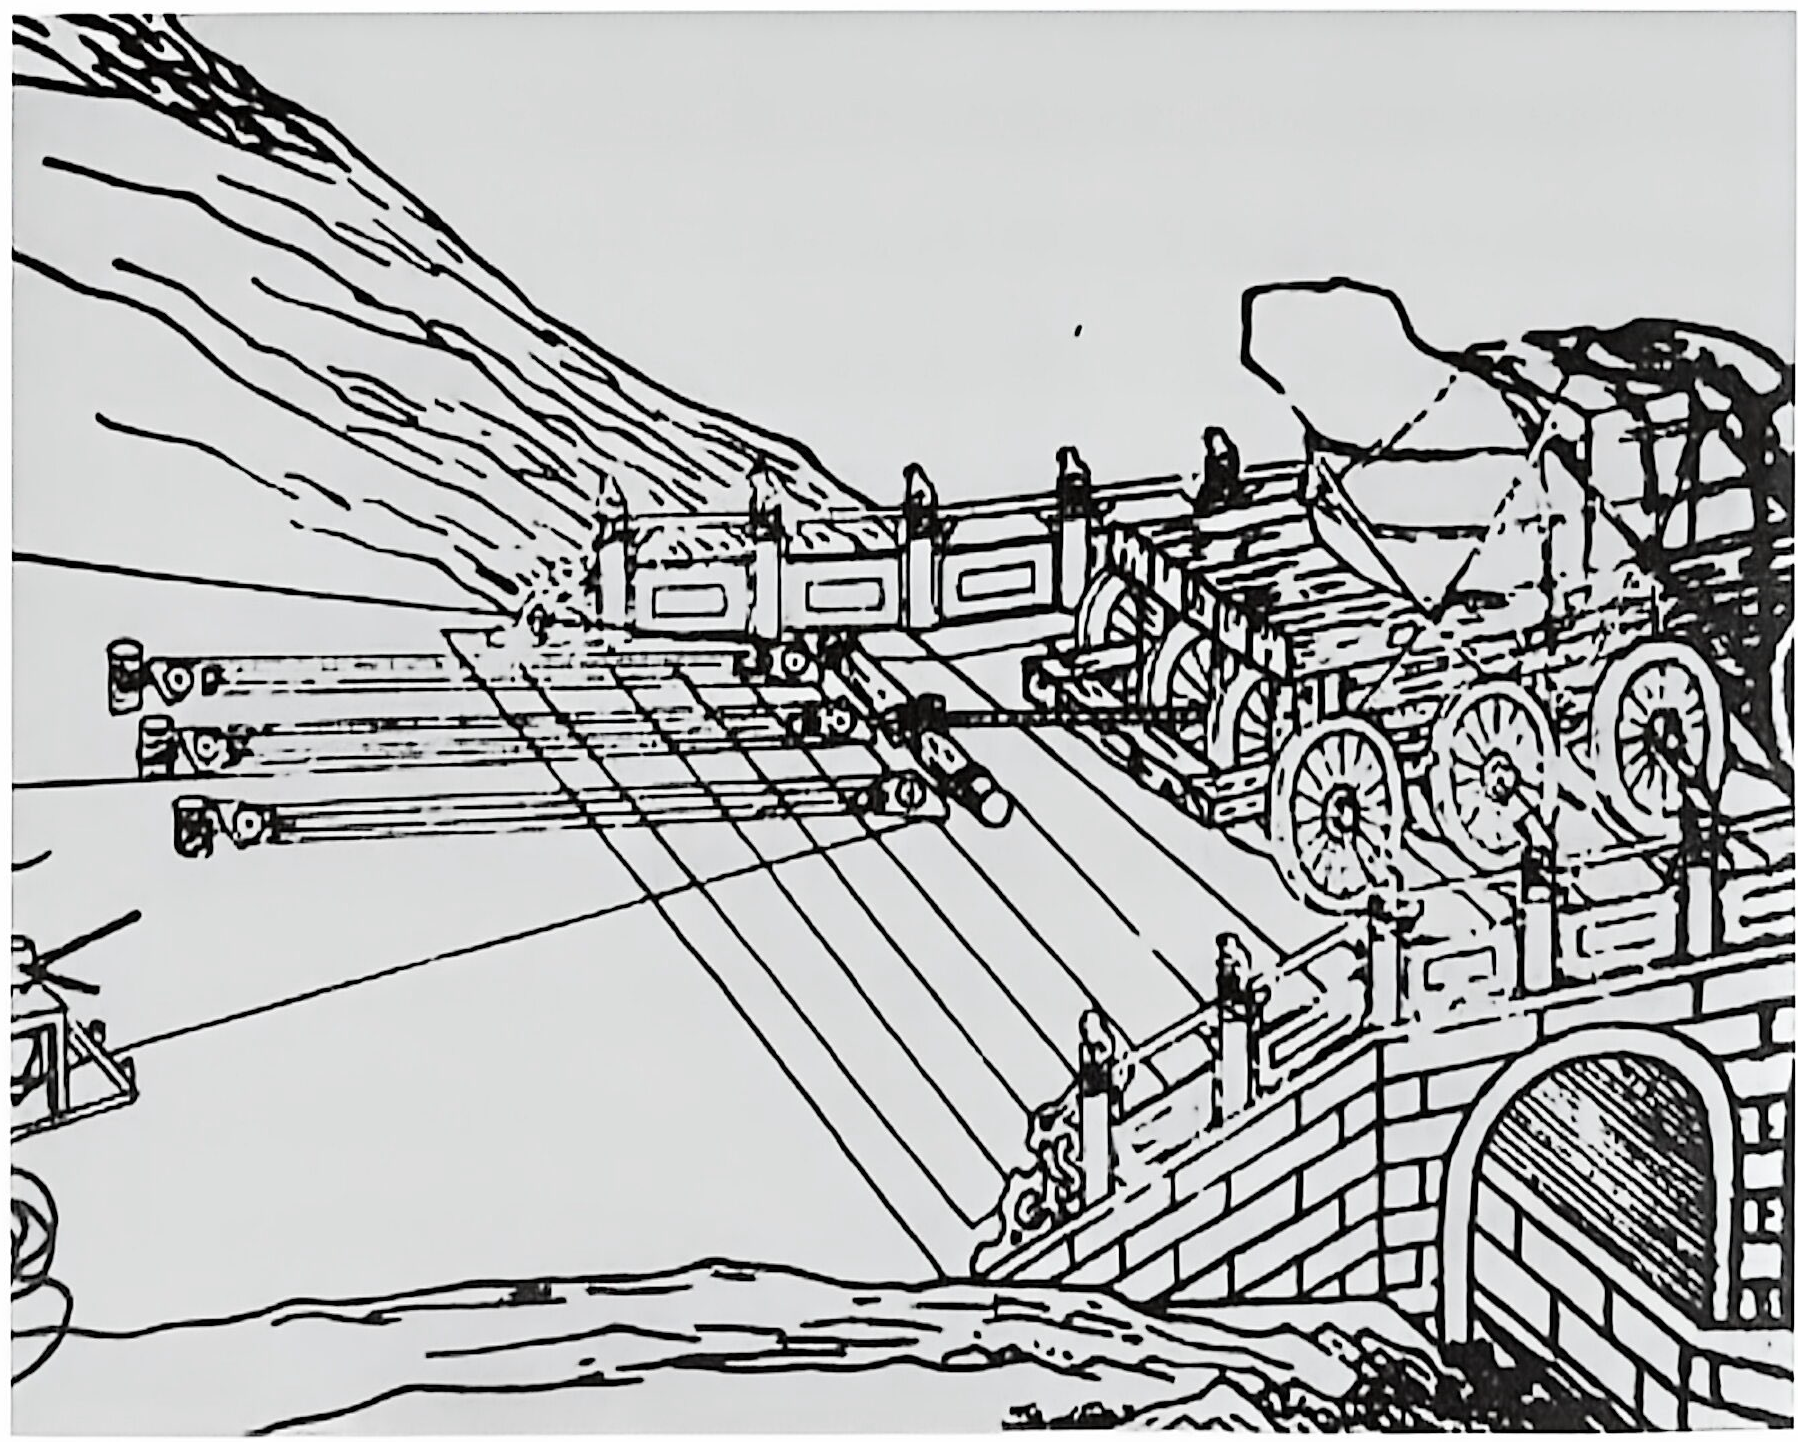
\includegraphics[width=\linewidth,height=.76\textheight,keepaspectratio]{assets/figures/verbiest-stone-transport.png}
\caption*{图3.1\quad 南怀仁石料牵引图}
\BookFloatNotes{图片来源：韩琦、吴旻校注，《熙朝崇正集熙朝定案（外三种）》，86。}
\end{figure}%
\par
% 原书页码：087；段落
后来1673年三藩之乱开始后，清朝的大炮辎重，无法进人浙江、%
福建等南方山地，也很难发挥作用。康熙委托南怀仁负责解决这个难%
题。南怀仁在短时间内对大炮制作以及运送方面做出了革新。他造出%
了小巧的大炮，还在大炮下安装了一组轮子，这一武器革新为平定三%
藩发挥了关键作用。南怀仁的炮造好以后，在郊外演习，康熙带着满%
朝文武观看，大炮的威力和准确性立时让朝廷上下官员叹服。南怀仁%
是康熙的人，他的大炮造得好，也是给康熙长脸。造炮以后，康熙又%
硬塞给南怀仁一个工部侍郎（仅次于工部尚书的职位）的官衔。据记%
载，康熙朝大小炮共造了905门，其中超过一半都是南怀仁造的。\NoteRef{3}{53}%
鸦片战争后，人华的欧洲人发现南怀仁造的大炮做工精致，图案雕刻%
有文物价值。八国联军侵华时，欧洲国家专门找到已经废弃的南怀仁%
大炮，把他们运回欧洲当文物。现在在罗马、柏林、伦敦、维也纳和%
布达佩斯等地博物馆都有专门收藏南怀仁造的大炮，他的名字就刻在%
炮身上。\NoteRef{3}{54}%
\par
% 原书页码：087–089；段落（跨页续段）
南怀仁还在北京制造出了世界最早的四轮蒸汽推动的可以控制方%
向的汽车。车身动力来自于车身中间架起的一个炭盆烧出的蒸汽。南%
怀仁把他制作汽车每一个部分用的材料、制作步骤都详细记录下来，%
让人带回欧洲，并在1687年出版。\NoteRef{3}{55}南怀仁没有具体记录车是哪一年%
制造完成的，但根据他书中所写的其他时间推算，应该是在1670年%
代中期就已完成。这比牛顿1688年提出的蒸汽车构想要早十多年。%
南怀仁和牛顿的设计相比，车的动力驱动部分，也即通过炭盆烧出蒸%
汽用以驱动的想法是一样的（图3.2和图3.3）。南怀仁当时已经把实%
物做了出来，车可以运行大约一小时，直到蒸汽用完。而牛顿那时提%
% 原书页码：088；图表（图题／表题所在页）
\begin{figure}[tbp]\phantomsection\label{fig-107-0}
\centering
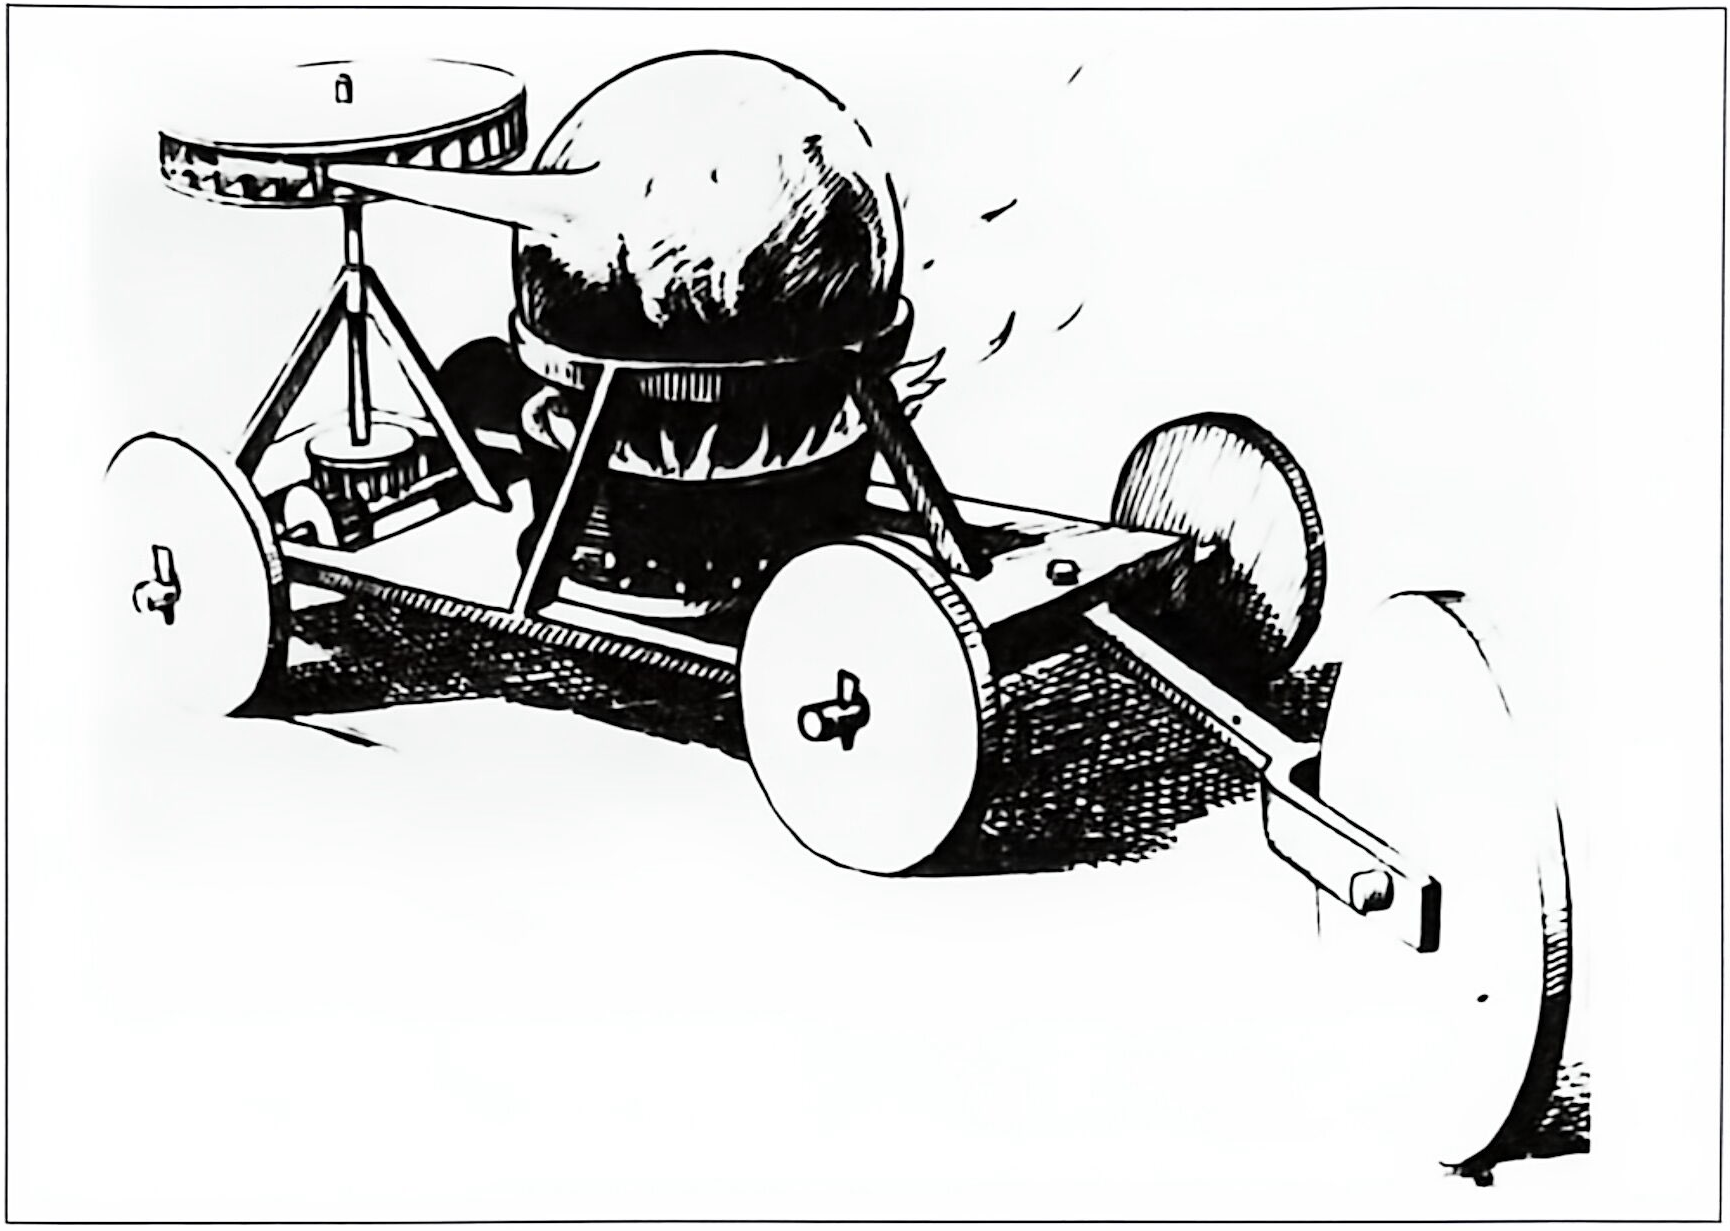
\includegraphics[width=\linewidth,height=.76\textheight,keepaspectratio]{assets/figures/verbiest-vehicle.png}
\caption*{图3.2\quad 南怀仁车模型图}
\BookFloatNotes{图片来源：\url{https://www.jesuiten.org/news/jesuit-erfand-das-erste-automobil-der-weltgeschichte}}
\end{figure}%
% 原书页码：088；图表（图题／表题所在页）
\begin{figure}[tbp]\phantomsection\label{fig-107-1}
\centering
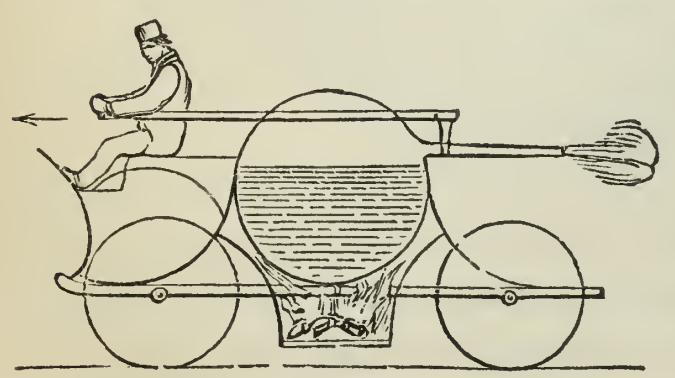
\includegraphics[width=\linewidth,height=.76\textheight,keepaspectratio]{assets/figures/newton-steam-car.png}
\caption*{图3.3\quad 牛顿1688 年提出的蒸汽车构想图}
\BookFloatNotes{图片来源：Sewell, John, Elementary Treatise on Steam and Locomotion, 244.}
\end{figure}%
出的仅仅是一个构想。南怀仁在蒸汽动力以及汽车发展历史中的位置，%
最近几十年逐渐被西方科学史家认可。南怀仁的比利时家乡博物馆还%
专门按照他的记载复制出一个模型来。南怀仁在书中还提到，他还做%
过蒸汽推动的船，船试航的时候还请了康熙的大哥来观看。\NoteRef{3}{56}可惜的是，%
船是怎么建构的，他没有细写，只提到用的是和他的蒸汽车推动一样%
的原理。尽管南怀仁不知道后来的蒸汽时代以及蒸汽动力对世界产生%
的改变，但他在书中已经预感到用蒸汽推动将是一场大的运输革新。\NoteRef{3}{57}%
西方科学史家相信南怀仁确实做出了蒸汽车，很重要的一个原因是南%
怀仁背后有强大的大清工部支持。这个蒸汽车能做出来，除了构想以%
外，对铁艺和木艺两方面都有很高要求。当时的工部是世界上少有的%
能在两方面都给予南怀仁支持的机构。%
\par
% 原书页码：089–090；段落（跨页续段）
十七、十八世纪，欧洲王公贵族有支持科学研究的风尚。各学%
科的科学家很多都依附于各地的达官贵人做研究、做实验。对于王%
公贵族来说，自己支持的科学家做出了成绩，是一件很有面子的事。%
南怀仁在送回欧洲出版的科技书籍中，标题部分就明确写出，他是%
在康熙皇帝的关照支持下做的各种科学实验。后来欧洲一直认为康%
熙是东方的开明君主，就源于各种关于康熙支持西方科学的报道。\NoteRef{3}{58}%
17世纪七八十年代，荷兰、葡萄牙、俄罗斯等国都派有使节来华，%
由于有传教士翻译，双方可以比较深人地交流。康熙一方面作为君%
主，会在礼部安排下，走完各种接待国外使臣的步骤。但他还会在%
正式接待结束后，把使节招到内廷交谈。当然交谈也都是传教士在%
做翻译。\NoteRef{3}{59}荷兰使节就很惊讶于康熙的科学素养。康熙不仅问了荷%
兰的地理情况，还问他荷兰的经纬度。也是因为康熙对学术的崇尚，%
后来法国国王在选派传教士到中国时，还将学术水准作为一个遴选%
门槛。%
\par
% 原书页码：090–091；段落（跨页续段）
康熙跟着南怀仁学习西学，是在皇宫内廷中进行的，学习中的各%
种具体事务是康熙的内务府在安排。尽管清朝正史中记载的都是南怀%
仁制作日历、观测天象以及制作大炮这些“公”事，但是南怀仁和康%
熙的私交才是令当时满朝文武称奇的。南怀仁比康熙大三十一岁。铲%
除鳌拜势力的1669年，南怀仁四十六岁，康熙十五岁。从南怀仁写给%
欧洲的信函中，可以看出他是把康熙当成自己的一个聪明学生在看待，%
字里行间能看出他对康熙是有真感情的。在他1682年春跟随康熙去%
东北祭祖的旅行记述中，就流露出他得意于康熙对他的各种照顾。祭%
祖前一年的冬天（1681年12月），清朝大军进人昆明，吴三桂之孙吴%
世璠兵败自缢，自此持续了八年的“三藩之乱”终于结束。这一次祭%
祖，二十八岁的康熙是去告慰满人列祖列宗的。康熙组织的祭祖队伍，%
阵容庞大，有七万人的规模。整个祭祖行程距离北京上千公里，一直%
到吉林松花江边上。据南怀仁记载，出了盛京（沈阳）后，很多地方%
都已经荒芜。只有沿途偶尔出现的一个个废弃村庄的遗迹，才仿佛显%
示满人曾经在这里居住过。满人打仗的传统是自带武器干粮，战胜得%
来的战利品也归自己所有。满人远征以旗为单位，出发的时候一家男%
女老少都跟着走，后来随着军队的胜利，满人也就迁徙去了他们占领%
的地方，很多人没有再回东北。康熙的回乡大军也遵循满人的老传统：%
以家为基本单位，马匹食宿自理，各旗分别自行安排扎营地。康熙选%
了十几匹他自己的马给南怀仁用，把南怀仁交给他的舅舅佟国维照顾，%
让他负责南怀仁的食宿。在康熙的安排下，南怀仁和佟国维同一桌吃%
饭，同一大帐住。整个远行没有作战的压力，又是出来庆祝胜利的，%
整体安排更像今天的户外野营郊游。康熙白天打猎钓鱼，遇到好的食%
材，还派快马送回京城孝敬孝庄太皇太后。晚上，生起篝火，康熙和%
皇亲国戚达官贵人围坐在一起，在浩瀚的夜空下，听南怀仁讲星星。%
在座之人，除了南怀仁，就属康熙最懂星空了。用南怀仁的话说，康%
熙也正好可“夸示自己的学问”。\NoteRef{3}{60}%
\par
% 原书页码：091；段落
在路上，朝鲜人还给康熙进献了活的海豹。康熙当时没有见过，%
问南怀仁欧洲知道这种动物么。南怀仁说知道，还告诉康熙他在自%
己编辑的关于鱼类的书籍中画过海豹，介绍过海豹的基本习性。康%
熙半信半疑，让快马回京城把书取来印证。在看到书上果然有介绍%
后，康熙表示很满意。\NoteRef{3}{61}后来，康熙带了一小队人去捕捞松花江中最%
著名的鲟鳇鱼，也把南怀仁带上。鲟鳇鱼大的超过两米，重两百多斤，%
自宋朝起就是有名的贡鱼。可惜的是康熙一行连遇几天大雨，不仅%
没有捕到鱼，回程也受影响，一路泥泞。在南怀仁的记录中，有一天，%
早上可以走过去的小溪回程时已经涨水变成一条河了。当时只有一%
艘小船可供渡河，帐篷食物都在对岸，过不去河就意味着要在泥泞%
中饿着肚子露宿一晚。康熙带着太子和几个权贵乘船先渡河，渡到%
一半，船又调头回来。等船的人都觉得奇怪，纷纷猜测原因，结果%
原来康熙是专门回来接南怀仁的。这一下让焦急等待的满人，切实%
感受到了南怀仁和康熙的关系。后来，又遇到差不多的情况，皇帝%
总要带着南怀仁先走，康熙的舅舅佟国维不干了，说南怀仁是他照%
看的人，要带走南怀仁就要把他一起带走。康熙却说让南怀仁以后%
行程就跟着他，不用舅舅再照顾了。%
\par
% 原书页码：092；段落
按中国传统政治来说，能够近距离接触皇帝就是特权。这个特%
权其实有一个不是官职但又有很重分量的头衔：“御前行走”。比这个%
差一点的是“内廷行走”，再差一点的是“乾清门行走”。这几个“行%
走”在政治上的不同分量，就是根据距离皇帝的远近来区分的。南%
怀仁与康熙的接触已经超过了“御前行走”。他和后来的传教士人宫，%
走的都是内务府专用的西门，这道门一般大臣都是不能用的。大臣%
人宫是走南边的太和门，然后再从乾清门进人内廷，完全是不一样%
的路线。%
% 原书页码：092；标题
\subsection{传教士带给康熙的世界}
\par
% 原书页码：092；段落
南怀仁除了教授康熙具体的知识以外，还深深影响了康熙对世界%
的认识，从而影响了大清后来一百多年北方和西北方向的战略部署。%
南怀仁给康熙普及了欧亚地理知识，特别是俄罗斯在欧亚大陆上的角%
色。康熙平定三藩后，首要目标是平定西北和北面还没有归顺的蒙古%
部落。解决蒙古问题，就要处理和俄罗斯的关系。南怀仁告诉康熙，%
当时俄罗斯正在西线与奥斯曼土耳其作战，让康熙明白俄罗斯也无意%
在东线与清朝为敌。这为康熙最后制定与俄罗斯和谈来解决蒙古问题%
的战略决策提供了关键信息。%
\par
% 原书页码：092–093；段落（跨页续段）
1676 年俄罗斯大使斯帕法里（Nikolai Gavrilovich Spathari, 1636—%
1708）率领一百五十人组成的庞大使团入华，在北京停留了四个月时%
间，南怀仁是翻译。斯帕法里这次还带来了两封明朝皇帝发给俄罗斯%
的信。一封是以永乐皇帝名号发的，一封是以万历皇帝名号发的。这%
两封信用中文写成，但俄罗斯朝野上下没人懂中文，所以斯帕法里把%
信带到北京，希望把信翻译成拉丁文。俄罗斯使团有带信到北京来寻%
求翻译的想法，就是他们知道康熙的朝廷里有传教士。同时斯帕法里%
还提议以后双方的正式交流语言为俄文、满文和拉丁文。俄国发出的%
函件为俄文和拉丁文，而清朝的回复用满文和拉丁文。康熙让议政王%
大臣会议讨论，最后同意了。拉丁文应该是16—18世纪环球航行以后，%
全球化中各国参与世界交流共同使用的语言。清朝正好有传教士在，%
也就很自然地融入这个世界体系中了。据统计，从1676年起到1730%
年，传教士为清廷共翻译了110封拉丁文的公函。\NoteRef{3}{62}%
\par
% 原书页码：093；段落
斯帕法里是学者，他早年在希腊接受教育，精通包括阿拉伯语%
在内的九种语言。他和南怀仁一见如故，惺惺相惜，他们用拉丁文%
长谈了很多次。南怀仁向斯帕法里透露了很多清朝内部运作的信息，%
以及他的理解。同时斯帕法里也给南怀仁讲了很多他对俄罗斯政局%
的看法。\NoteRef{3}{63}%
\par
% 原书页码：093；段落
斯帕法里使团除了在通信语言上与清朝达成了一致，其他谈判问%
题都没有结果，因为清朝坚持要求俄罗斯以藩邦附属国地位与其谈判，%
这让斯帕法里觉得完全不可理解，当然也没有同意。清朝礼部坚持使%
团行跪拜叩头的礼节，斯帕法里也表示难以接受。\NoteRef{3}{64}%
\par
% 原书页码：093–094；段落（跨页续段）
康熙在传教士的影响下，早就明白西方国家交流中的平等观念。%
但大臣坚持既定的传统规矩，他作为皇帝也不能干预。皇帝和大臣在%
朝廷制度下是互相制约与平衡的关系，大臣按照皇帝制定或说认定的%
规章制度办事，那么皇帝就必须要尊重大臣按章行事。黄仁宇在《万%
历十五年》中称明朝皇帝是体制运作中的一个部件（instrument），就%
是这个意思。\NoteRef{3}{65}清朝皇帝在继承明代的朝廷制度以后，也经常感到制%
度对他们个人权力的限制。而康熙和后来的雍正面对这种限制，想到%
的办法不是改革朝廷制度来加强皇权，而是绕开朝廷制度来私下办理。%
这是本书后面会涉及的内容。比如康熙后来接待一些外国使团，就直%
接绕开了礼部和理藩院这些朝廷部门，而安排他的内务府来承办，以%
此来摆脱各种条条框框的限制。%
\par
% 原书页码：094–095；段落（跨页续段）
尽管清朝和俄罗斯使团没有达成什么具体协议，南怀仁还是在和%
斯帕法里的交流中，验证了他心中的一个想法，就是从欧洲经由俄罗%
斯陆路来华的路线是可能实现的。当时全球航线已经形成，但是航道%
主要被葡萄牙、西班牙和荷兰几国垄断。天主教传教士尽管名义上都%
是教皇派出的，但是每个传教士在欧洲各属于不同国家，因而欧洲各%
国传教士入华前，还要得到当时几个海上称霸国家的支持。像荷兰已%
经是新教国家，和天主教国家在欧洲就有分歧，加上欧洲各国的政治%
关系又在不停变化，对一些有志来华的传教士来说，走海路有许多麻%
烦。当时的海路航行风险也很大，有不少花很大精力培养出来的来华%
传教士因为各种原因死在了路上。顺治时代，罗马就派出过传教士探%
索陆地线路，传教士白乃心（Johann Grueber，1623—1680）在汤若望%
的经济支持下，走西宁、拉萨，翻越喜马拉雅山，通过尼泊尔加德满%
都到印度，开辟陆地线路。尽管白乃心最后回到了罗马，还把中国西%
藏、尼泊尔的故事讲给了欧洲，但是北印度有一段不让西洋人通过，%
他只能走海路，也就是说他没能找到一条传教士可以通行的陆地线路%
到中国。他最后向罗马汇报的结果是这条线路太苦，沿途各种势力盘%
踞，不确定性与海路不相上下。\NoteRef{3}{66}所以南怀仁把希望放在了俄罗斯线%
路上。他认为如果得到俄罗斯的允准，可以很大程度上方便欧洲传教%
士人华，而且陆路的安全性也更好。%
\par
% 原书页码：095；段落
南怀仁的这个想法得到了教皇的认可，同时也得到了康熙的支%
持。法国国王路易十四（1638—1715）也认为南怀仁的想法是可行的，%
他派了两队耶稣会传教士前往中国，一组人走的陆路，一组人走的%
海路。走海路一组到达了中国，这在后面的章节中会讲到。走陆路%
的一组在1687年1月到达莫斯科。因为在两年前的1685年，莫斯%
科收到大清发来的边界谈判文件（文件有拉丁文翻译），俄罗斯对谈%
判条款很不满意，同时认为耶稣会传教士帮助清朝谈判，而且还帮%
助清朝制造大炮和俄罗斯作战，这些都是背叛西方的举动。于是俄%
罗斯直接把耶稣会告到了罗马，要教皇给个说法。\NoteRef{3}{67}在这个背景下，%
俄罗斯没有给两位法国耶稣会传教士颁发通行的文件。这一组人没%
能继续他们的行程。他们带给康熙的信件也没送到中国，这封信现%
在还保存在法国。红票中提到的四位传教士中的薄贤士就是第一批%
探索陆路通道的法国传教士之一。虽然陆路没能走通，最后他还是%
从海路到达了中国。%
\par
% 原书页码：095–096；段落（跨页续段）
当时从欧洲进人俄罗斯最关键的一个国家是波兰。1680年代的%
波兰国王约翰三世（King of Poland, John Ⅲ）是欧洲的风云人物，他%
与奥地利组成的联军在1683年维也纳之战中战胜了锐不可当的土耳%
其军队。约翰三世也是热衷文化的君主，他的私人图书馆在当时欧洲%
都是很有名的。按中国说法，约翰三世是文治武功俱佳的君主。欧洲%
现存的很多油画中还有约翰三世的画像，都是英明神武的姿态。由于%
约翰三世和俄罗斯有各种协议，当时欧洲教会都把打开俄罗斯路线的%
希望寄托在约翰三世身上。南怀仁1685年发了一封信到德国耶稣会%
分部，请他们把信转交给约翰三世。在这封转交的信中，就附有康熙%
祝贺约翰三世取得维也纳之战胜利的贺词。贺词原件已经不存，据记%
录是康熙毛笔手书。约翰三世和南怀仁的通信还有一部分存世。在其%
中一封给南怀仁的信中，约翰三世附了一张自己的肖像画，让南怀仁%
转交给康熙，表示对康熙恭贺他胜利的感谢。\NoteRef{3}{68}约翰三世对南怀仁和%
康熙请求开辟俄罗斯路线的建议很上心。1686年，在波兰和俄罗斯%
签订的一份协议中，约翰三世要求在条约中加人“教会人员可以通过%
莫斯科领土前往中国”的条款，但俄罗斯拒绝了这一条。俄罗斯谈判%
方称，条约中已有持波兰国王发放文件人员可以在俄罗斯通行的条%
款。也就是说，波兰国王要支持传教士到中国，通过发放文件就可以%
帮他们通过俄罗斯。\NoteRef{3}{69}后来真有一批波兰耶稣会传教士报名，希望通%
过这个条款借道俄罗斯到中国，不过俄罗斯方面以人华线路不安全为%
由，把到来的波兰传教士都劝返了，归根结底，俄罗斯还是不希望打%
开这条通路。%
\par
% 原书页码：096–097；段落（跨页续段）
路易十四和约翰三世积极呼应南怀仁，希望和大清康熙皇帝建立%
关系，除了国家利益考量以外，还因为这两位都是热衷学术并且对东%
方文化很感兴趣的君主。约翰三世的华沙宫殿中，有专门的中国馆，%
还有中国的花瓶。开辟陆地线路，当时有许多学者加人讨论其可行性%
以及可能的路线。著名的德国学者莱布尼茨就和波兰国王私人图书馆%
馆长有很多讨论路线的通信。其中几封信中，二人还在探讨为什么俄%
罗斯不让传教士借道去中国。二人猜测，俄罗斯是怕欧洲国家开辟了%
陆地线路后，打破俄罗斯对东北亚贸易的垄断。对当时欧洲的学者来%
说，东北亚以及西伯利亚很多地区都是未知区域，他们都很有兴趣了%
解那里的人和事。%
\par
% 原书页码：097；段落
南怀仁和康熙除了写信以外，对建立陆地线路也有切实的行动。%
在南怀仁建议下，康熙派出当时在钦天监内给南怀仁做助手的意大利%
闵明我神父作为他的特使去往欧洲。作为康熙特使，闵明我神父有两%
个任务：一是从欧洲方向联系俄罗斯，他当时带着兵部发给俄罗斯的%
信函；二是看有没有可能打开陆路通道。闵明我神父1686年冬离开中%
国，到达罗马汇报完中国教会的情况后，就寻求罗马教廷的帮助以打%
开陆路通道。他还动用各种私人关系，希望能说服1682年登基的彼%
得大帝。他在罗马和莱布尼茨见过面，拜托莱布尼茨帮忙联系劝说和%
他有私交的彼得大帝。\NoteRef{3}{70}%
\par
% 原书页码：097；段落
清朝还请1686来朝的荷兰使节充当调停人，让他返回欧洲后，通%
过荷兰的渠道帮助清朝与俄罗斯交流，希望尽快与俄罗斯达成边界共%
识。荷兰带给俄罗斯的信是以大清兵部名义发出的。\NoteRef{3}{71}%
\par
% 原书页码：097–098；段落（跨页续段）
康熙有这种大国互动的世界格局，就是在南怀仁的帮助下逐渐形%
成的。其实在1680年代，清朝和俄罗斯在东北还不断有军事冲突，%
如比较有名的雅克萨之战。但在南怀仁的指点下，康熙明白那些冲突%
对中俄两方来说都不是核心利益所在，两国完全有可能达成一致。所%
以我们看到，在1680年代，清朝廷官方在不停说硬话，还在派军队，%
而康熙又同时在寻找各种渠道和俄罗斯谈判。1686年以后，康熙和%
彼得大帝双方都有很强意愿签订条约，这样二人好放手来干自己心目%
中真正的大事。1686年俄罗斯加人了奥地利、波兰和威尼斯组建的%
神圣联盟（Holy League），共同抵御奥斯曼土耳其帝国。同时俄罗斯%
在这一时期还在克里米亚打仗（1687、1689年）。另外俄罗斯跟瑞典%
也处于敌对之中。同时，清朝西北面的噶尔丹汗日趋强大，1686年%
开始吞并蒙古其他部落，康熙几次发出警告，噶尔丹都没有理会。康%
熙知道这一时期噶尔丹的许多战争都得到俄罗斯支持。对于康熙来%
说，跟俄罗斯签订条约，他才好放手来对付噶尔丹。清朝和俄罗斯%
在1689年签订的《尼布楚条约》就是这一时期双边关系发展的结果。%
而这个条约从开始谋划，到最后签订，康熙都是站在近代国家平等观%
念下在思考。思考的过程也接近现代国家谈判思维，考虑的是利益取%
舍，没有在一些虚无的礼仪称谓问题上费心思。康熙在思维方式和战%
略眼光上都远超其朝廷里的大臣。这一切应该说都和南怀仁的培养以%
及他给康熙提供的信息分不开。%
\par
% 原书页码：098–099；段落（跨页续段）
南怀仁对康熙的价值，从他死后的恩荣上也可看出端倪。康熙%
赐给南怀仁“勤敏”的谥号。对于谥号，大清的规矩是必须一生勤恳，%
没有大的污点才能获得。而且正常情况下，只有一品大员会有谥号。%
不是一品的，需要皇帝钦赐。南怀仁没有做过一品大员，所以他的%
谥号是康熙钦赐的。对比之下，康熙早年的宠臣索额图和明珠，都%
因为后来这样那样的问题，没有获得谥号。能得到钦赐的谥号，在%
康熙一朝是很难得的恩宠。而且谥号是有品次的。表明品次的是谥%
号的首字。南怀仁谥号的首字是“勤”字，而当时最有名的拥有“勤”%
字谥号的是佟图赖，也就是康熙的外公。佟图赖是八旗正蓝旗汉军%
都统，带领军队从东北一路打到广西，为满人夺取天下立了大功，%
最后获得的谥号是“勤襄”。南怀仁最后的谥号可以和佟图赖并立%
于“勤”字档，在康熙一朝来说是极高的评价。最后南怀仁的墓碑%
上还是汉满双语并立，使用满语说明康熙把南怀仁当成自己人。南%
怀仁在1688年去世，中俄双方都认可1689年最后的条约能够签订，%
南怀仁当居首功。%
% 原书页码：099；标题
\subsection{《尼布楚条约》签订}
\par
% 原书页码：099；段落
1688年1月28日，南怀仁在北京去世。六年前，利类思神父已%
经去世。这样，康熙朝宫中第一代传教士已全部去世。当时北京能在%
康熙身边经常出现的还剩下徐日升、安多两位神父。徐日升神父是葡%
萄牙人，在南怀仁引荐下，1673年进入宫中。他擅长音乐，把西方音%
乐介绍给了康熙。徐日升神父和康熙的儿子们相处融洽，后者把他当%
成家里人。康熙的家训里还有大皇子拿徐日升神父的大胡子开玩笑，%
被康熙制止的故事。\NoteRef{3}{72}安多神父是比利时人，1685年人京，在南怀仁%
引荐下成为康熙的西学老师。而南怀仁在钦天监的位置则传给了闵明%
我神父。闵明我一直是南怀仁的助手，精通天文历算。南怀仁去世时，%
闵明我被派回了欧洲未返，但钦天监的位置一直给他留着。直到1694%
年他返回北京以后，才正式顶了南怀仁的缺。%
\par
% 原书页码：099–100；段落（跨页续段）
南怀仁去世后十天，也就是1688年2月7日，法国国王路%
易十四派出走海路入华的白晋、张诚、洪若翰（Jean de Fontaney，%
1643—1710）、李明（Louis le Comte，1655—1728）和刘应（Claude%
\space%
de Visdelou，1656—1737）五位法国耶稣会传教士终于抵达了北京。\NoteRef{3}{73}%
尽管五人未能见到南怀仁，但是在他们六个月前到达宁波的时候，%
就已经感受到南怀仁在清朝的影响力。按照清朝规定，西洋人人华%
只能从广东进人。但是从澳门到广东的人华路线多年来都掌握在葡%
萄牙人手中。这五位法国传教士为了回避葡萄牙人，选择了从宁波%
进人中国。当时的浙江巡抚金见五位西洋人突然来访，上书朝廷，%
询问应该如何处理。管理西洋人的礼部给出的回复是严格执行现有%
条例，不允许传教士从宁波进人，责令他们离开，同时要求巡抚严%
惩带他们到宁波的商人。不过六天后，礼部这一回复被康熙否定了。%
康熙声称这几人懂得历法，让他们来京，听候差遣。据传教士记载，%
浙江地方官得知康熙让他们进京后，亲自到他们的住处拜访，恭喜%
他们能够得到皇帝恩宠接见。由于他们是康熙钦点要接见的人，所%
以从浙江赴京一千多公里的路上，他们得到了沿途各处地方官员的%
款待和照顾。\NoteRef{3}{74}法国传教士知道这一切都是康熙的面子，当然也清楚%
这一切都是南怀仁在华几十年兢兢业业深耕的结果。%
\par
% 原书页码：100；段落
由于南怀仁的缘故，康熙对这几位新来的传教士都很信任。康熙%
把白晋和张诚两位神父选留在宫中。他们二人的生活起居由康熙的内%
务府负责打理。据白晋记载，每天早上，内务府派人和马把他们接人%
宫中，然后指派专人帮助他们突击学习满语。吃和住也都是内务府负%
责安排。\NoteRef{3}{75}当时耶稣会传教士到世界各地去传教，都是为了奉献上帝，%
做好了外出吃苦的心理准备。这几位法国传教士没想到，到了中国，%
被一路款待；到了北京，就能入宫行走，享受皇家待遇，这些都远超%
他们预期。%
\par
% 原书页码：100–101；段落（跨页续段）
康熙对法国传教士的信任优待其实是对南怀仁信任的延续。仅仅%
过了一年，1689年与俄罗斯进行边界谈判，康熙就把张诚派入谈判%
队伍中。张诚此时汉语和满语都没有学通，但康熙知道他是人才，还%
是派他去，还赏赐给他专门的衣服，要舅舅佟国纲照顾他的生活起%
居。这支谈判队伍是索额图和佟国纲领衔率队。毕竟张诚来华时间太%
短，索额图和佟国纲都和他不熟悉，他们对如何使用张诚以及张诚的%
忠诚等有疑虑。后来他们想到的办法是，他们只与使团里另外一位神%
父——老熟人徐日升交接联系，而把张诚安排在徐日升神父手下。这%
样一来，要是张诚在出使之中出了什么问题，就要徐日升负责。%
\par
% 原书页码：101–102；段落（跨页续段）
新来的张诚，知道俄罗斯在欧洲那边已经焦头烂额。它陷在克里%
米亚地区已经好几年，同时还在和瑞典以及奥斯曼帝国争夺波罗的海%
的出海控制权。了解这些信息，相当于知道了俄罗斯的底牌，知道俄%
罗斯有很强的意愿和清朝解决东北亚地区的边界问题。只有把东北%
亚问题解决了，它才能放开手脚专心处理西面的问题。\NoteRef{3}{76}名义上索额%
图和佟国纲是清朝谈判代表，但其实两位神父才是谈判的实际代表。%
他们二人不是翻译，因为大部分谈判时间索额图和佟国纲都没有出%
席，是二位传教士直接去俄罗斯代表处，用拉丁文和俄罗斯代表谈判%
的。最后拟定的条约总共七条，主要在四个方面达成一致。条约的官%
方语言是拉丁文，同时有满文和俄文的版本。条约汉文版本是鸦片战%
争以后才翻译出来的。合约第一要处理的是边界问题。边界问题，最%
大的模糊地带是黑龙江以外西伯利亚地区划界问题。当时中俄双方对%
黑龙江以外的地区地理所知都很有限，两位神父也基本一无所知。双%
方谈判边界其实是在互相试探对方的底牌。当时俄罗斯代表问清朝准%
备要在哪里划界。两位传教士回来问索额图和佟国纲，二人提出边界%
需要划到Nos山脉处。Nos山究竟是什么地方，学界现在没有定论，%
但肯定在乌第河（Uda river）以外很远的地方。一说是上扬斯克山脉%
（Verkhoyansk Range），还有说是俄罗斯领土最东北，接近阿拉斯加的%
部分。\NoteRef{3}{77}这个提议让俄方感觉完全不可接受，断然拒绝。根据徐日升%
神父的日记记载，两位传教士回来问索额图和佟国纲是否知道Nos山%
脉在哪里，结果二人说不知道。\NoteRef{3}{78}同时在清朝带出来的地图上也没有%
这个地方。清朝的地图最远处就在黑龙江区域。\NoteRef{3}{79}张诚告诉两位大员，%
根据他看到的俄罗斯地图，按照经纬度计算，他们要的Nos山离北京%
有约四千公里（800里格，1里格约等于4.8公里。而北京距离哈尔%
滨约1200公里）。\NoteRef{3}{80}两位大员听后，只是互相对视了一眼，立刻决定%
不再漫天要地了。\NoteRef{3}{81}后来清朝提出把边界定在黑龙江以外的乌第河附%
近。黑龙江区域到乌第河区域不通航，大山阻隔。清朝军队其实从来%
没有到达过乌第河区域（起码没有任何记载）。\NoteRef{3}{82}只是黑龙江周围的满%
人中流传着一些关于乌第河区域的传说，在以前的贸易中知道那边有%
一些珍贵的动物，传说那边还有一些神奇的大鱼。\NoteRef{3}{83}两位大员只听过%
一些那边的传说，实际所知甚少，而且连乌第河区域的地图也没有。\NoteRef{3}{84}%
不过好歹他们还是讲出了那边的物种，给出了满人需要去那边捕猎这%
个理由。在两位传教士的争取下，俄罗斯代表认为可以接受，最后双%
方同意乌第河区域为中间地带，双方的人都可以进人这一区域。\NoteRef{3}{85}应%
该说俄罗斯谈判一方，对那边情况也所知不多，只是他们拿来的地图%
上可以看到那个区域。另外清朝要的乌第河区域比之前要的Nos区域%
小了很多。按俄罗斯的说法，Nos山的最南面，离乌第河区域都至少%
还有十周的行程。\NoteRef{3}{86}根据现代学者的计算，几天之内，清朝对领土的%
主张缩小到原来的五十分之一。\NoteRef{3}{87}东北端的边界谈妥以后，其他的边%
界双方都相对熟悉，也就没有多少争议了。%
\par
% 原书页码：103；段落
条约第二部分是解决了人口归属问题。先前清朝和俄罗斯在东北%
的冲突，很多都是由于一些部族因为各种原因不满清廷的统治，跑到%
俄罗斯那边去了。之前很多次谈判，清朝都有一个叛逃重要人物名单%
交给俄罗斯，要求俄罗斯把上面的人交还回来，但俄罗斯拒绝配合。\NoteRef{3}{88}%
东北亚地广人稀，人就是重要资源。从国家利益上来说，俄罗斯是欢%
迎人口迁徙到它那一侧去的，所以它一直拒绝清朝的要求。这次双方%
在逃人问题上达成一致，约定条约签订前的逃人，双方就互相不追究%
了；以后的逃人，双方需要互相遣送。如果有超过十五人的团体潜逃%
越境，双方需要互相知会。在清朝八旗中，还有一个小团体是由俄罗%
斯人组成的，这些俄罗斯人是以前战争中的战俘，这个条约也意味着%
这些人不用再送回俄罗斯了。%
\par
% 原书页码：103；段落
三是贸易问题，双方都可以派人去对方国家贸易。这一条款当时%
认为是俄罗斯占便宜，因为清朝对去俄罗斯贸易没有多大兴趣。而俄%
罗斯根据这个条款，在北京驻扎了一个代办处，有点类似于今天的大%
使馆。各西方国家都很羡慕俄罗斯在北京的代办处。后来人华的教皇%
特使，也想在京城购置房产建一个类似的机构。这在后面的章节中%
会讲到。%
\par
% 原书页码：103；段落
四是俄罗斯永远撤出雅克萨，并拆除雅克萨的堡垒，把雅克萨的俄%
罗斯人撤回国，雅克萨归大清所有。1680年代，清朝和俄罗斯数次为%
争夺雅克萨开战，尽管战争规模不大，只是几千人级别的军事冲突，但%
始终是双方一个重大的争议问题。俄罗斯在这个问题上让步，让康熙%
和清朝赢得了颜面，清朝谈判代表索额图和佟国纲对此很满意。索额%
图也直接向两位神父许诺，以后朝中有事，尽管找他，他一定鼎力相助。%
\par
% 原书页码：104；段落
两位传教士一直对外声称二人只是清朝的翻译，因为他们不想%
得罪俄罗斯。当时教皇和俄罗斯是同盟，在共同抵御奥斯曼土耳其。%
他们写回欧洲的信件，也强调他们只是翻译，决策都是索额图和佟%
国纲两位官员做的。但实际二人对很多谈判细节有关键影响。康熙%
在使团出行前，专门和徐日升神父探讨过各种问题，应该是给过徐%
日升一个谈判底牌，告诉了他哪些是大清不能退让的问题。这一点%
从索额图和佟国纲对两位传教士意见的依赖上可以看出。同时根据%
俄罗斯使团回去后的报告，他们认为清朝在条约谈判中的一些意见%
是两位传教士的意见。当时俄罗斯使团还贿赂过两人。由于俄方贿%
赂物品算作使团开销，所以有详细记录。记录显示，其中有红酒、%
黄油、十五只鸡、四十只紫貂、一百五十只白鼬和两只黑狐狸。黑%
狐狸皮在当时极其贵重，俄方领队就穿了一件黑狐狸皮的衣服，张%
诚神父还专门夸赞过。\NoteRef{3}{89}%
\par
% 原书页码：104；段落
两位传教士并没有偏向俄罗斯，俄罗斯最后的报告说传教士就是%
偏向清朝。俄罗斯使团甚至找到随团的蒙古语翻译，与索额图直接对%
话，质问他那两位传教士坚持的是不是清朝使团的意思。\NoteRef{3}{90}在尼布楚%
谈判前一年（1688年），俄罗斯和清朝在色楞金斯克（现在俄罗斯境%
内）已经谈过一轮，\NoteRef{3}{91}所以他们大概知道清朝的底线。按照俄罗斯使团%
的报告分析，清朝使团对签订条款是很急迫的，反而是两位传教士从%
中作梗，在深度捍卫清朝利益。俄罗斯使团的分析大约是有道理的，%
索额图也确实担心无功而返，他后来也劝说两位传教士在有些地方可%
以让步。%
\par
% 原书页码：104–105；段落（跨页续段）
中俄这次条约签订是在打心理战，很多问题其实双方都没有预定%
底线，都是在互相探底，多一点，少一点，其实双方都能接受。\NoteRef{3}{92}上%
面讲到的西伯利亚地区边界谈判就是这种情况。而传教士比清朝官员%
更了解俄罗斯，同时他们在实际谈判中，根据俄罗斯的说词，察言观%
色，也能获得更多的信息，所以他们给俄罗斯人印象更强硬。当然%
传教士也想通过签订这个条约来表现自己。他们受到康熙的眷顾和恩%
宠，这是在欧洲都不可想象的，那里不会有多少国王或者王公贵族多%
看他们一眼。张诚在写回欧洲的关于这次行程的信函中，就很感慨地%
说，他何德何能，康熙皇帝竟然能如此信赖和恩宠他，把如此重要的%
任务交给他。\NoteRef{3}{93}当然有些人会认为这是写作中的套话，谦虚之语。张%
诚当时才三十四岁，一行人中他是最小的。而索额图和佟国纲都已%
五十多岁，纵横官场几十年，但他们一路都对张诚的意见很重视。从%
私人感情上，康熙对这些来华传教士而言是有知遇之恩的明主，所谓%
投桃报李，传教士也有心全力以赴为清朝谈判。从传教利益来讲，中%
国才是传教士需要传播福音的地方，他们当然要效忠清朝。后来彼得%
大帝看了条约以及使团报告中提及的传教士的表现，很生气，认为这%
些耶稣会传教士背叛了整个基督世界。当时正在开辟陆地线路去中国%
的耶稣会传教士其实已经在圣彼得堡建立了一个代办处，作为去中国%
的中转站。彼得大帝一怒之下，封了这个代办处，还把耶稣会所有传%
教士都赶出了俄国。%
% 原书页码：106；标题
\subsection{小结}
\par
% 原书页码：106；段落
现代数学中，代数几何大部分基础概念的汉语词汇，都是康熙那%
时候翻译出来的。康熙晚年在一次家庭聚会上，回忆说自已开始学习%
数学天文是在杨光先参劾汤若望的时候，\NoteRef{3}{94}也就是1665年左右。1665%
年是康熙五年，这时康熙十二岁，尚未亲政。%
\par
% 原书页码：106；段落
1665年，朝政还掌控在以鳌拜为首的四位辅政大臣手里。这一年%
是他们辅政的第五年。康熙当时还未成年，他的主要任务是学习。皇%
帝应该学习什么，是国政，是辅政大臣要安排的国家大事。前章已经%
提到过，恢复满人传统是辅政大臣时期的治国方针。这个方针也体现%
在康熙的学习安排中。康熙这时期的学习内容主要是满人传统的骑马、%
射箭、打猎这些技艺。当时礼部的官员很着急，曾经多次上书，奏请%
辅政大臣允准汉臣给康熙开蒙。对于这些奏请，辅政大臣没有驳斥，%
但也没有允准。第一次正面回复这些奏请的是康熙自己。在1669年%
铲除鳌拜势力后，十五岁的康熙命礼部尽快安排他学习汉文经典的各%
项事宜。这之前，他只跟宫中的太监简单学了点汉语。可以看出，辅%
政大臣对于文化经典并不重视，有意思的是，他们连康熙学习满文都%
没有做安排，反而是孝庄太后实在看不下去，让苏麻喇姑来教康熙%
满文。\NoteRef{3}{95}%
\par
% 原书页码：106–107；段落（跨页续段）
了解康熙早年的学习大环境后，就衍生出一个问题：连汉文经典%
都没有正规学习过的康熙，为什么能够学习数学，而且是西方数学？%
无论是满人传统还是汉族传统，皇帝都没有学习西方数学的先例。而%
且康熙学习过的日影计算，不仅需要数学知识还需要几何知识，这些%
知识不可能凭一时兴趣，一两天就能学明白，而是需要系统的数学学%
习。为什么耶稣会的传教士们会被允许接近康熙，而且教康熙这些数%
学知识?%
\par
% 原书页码：107；段落
接触皇帝在历史中从来不是一件容易的事情，面圣一直以来都%
是一种特权。住在深宫中的皇帝，只有很少一部分人能接触到。官%
僚系统尽管理论上有可能让一般人“上达天听”，但是实际操作中，%
不要说面圣，就是书写的奏疏能递到皇帝手里都是很困难的事。任%
何能够接触皇帝的渠道都是很珍贵的。为什么历史上总是有宦官弄%
权？就是因为宦官在皇帝身边，是那一小部分可以垄断接近皇帝渠%
道的人。%
\par
% 原书页码：107；段落
尽管如此，这些西洋来的传教士却一直可以在康熙朝的六十一年%
中私下接触到康熙。康熙年轻的时候，有些传教士可以说是每天都在%
他身边。长期以来，大都认为是康熙对西学感兴趣，所以经常接触传%
教士。这个解释明显颠倒了因果。如果不是因为先接触到了传教士，%
一个中国皇帝怎么可能对西学凭空发生兴趣?%
\par
% 原书页码：107–108；段落（跨页续段）
这里所谓的西学，主要是以数学为代表，纯理论性质的代数和几%
何。比如康熙去世前五年，在用满文写给皇三子的一封口谕中，要他%
问一位刚从欧洲来的传教士，到底欧洲数学家有没有找到新的方法来%
求解平方根和立方根。这就说明康熙知道老的方法，但嫌太笨了，所%
以想知道新方法。对这种问题感兴趣，是很纯粹的学术兴趣。康熙大%
约也是中国第一批接触到西方代数的人。传教士把代数书写好以后，%
直接呈给了康熙，说这是一种把数学问题变简单的方法。康熙外出离%
京时把这本书带在身边，当闲书看。但他没看懂，写了张条子传给宫%
内的奴才，上说：“朕自起身以来，每日同阿哥等查阿尔巴拉新法，最%
难明白。他说比旧法易，看来比旧法愈难。”\NoteRef{3}{96}康熙让宫里奴才去找北%
京传教士，让他们把书里问题写得再清楚明白一些。这里康熙说的“阿%
尔巴拉”就是代数Algebra的音译。康熙把数学当成出巡时的娱乐读物，%
这兴趣是不一般的，而且他的皇子阿哥们还跟他一起看。%
\par
% 原书页码：108；段落
“兴趣”这个词经常被大家用来解释人起意行动做事的原因，但往%
往没有注意到兴趣和兴趣之间的差异。比如一个人喜欢饮酒，喜欢美%
色，这些是天性，可以归结为自发产生的兴趣。但还有一些兴趣有很%
高的门槛，康熙感兴趣的数学就属于这一类。数学作为学问，有内在%
的逻辑和纯粹的美感，但要领略到这个美感，就得经过长时间的学习。%
理解这一点，就能明白康熙对西方数学感兴趣必然是先有传教士和康%
熙接触的因，然后才会有康熙对数学感兴趣的果。%
\par
% 原书页码：108；段落
从康熙小时候就在他身边的南怀仁，是引导康熙对西方学科感%
兴趣的“因”。南怀仁作为一个神父，性格和善可亲、平易近人，朝%
堂内外都喜欢他；同时他又博学多才，天文地理、动物植物、技术艺%
术，样样精通。南怀仁的科学著作放在当时的欧洲也是一流学者的%
水平。康熙跟着南怀仁这样的老师自然也受益良多。只是康熙和南%
怀仁的私下教学和交往属于内务府府中之事，清史中对他们交往的%
官方记录很少。%
\par
% 原书页码：108–109；段落（跨页续段）
当然也有可能是康熙有意避免史官记录他和传教士的往来。在他%
派出去和俄罗斯谈判的队伍里，一个汉官都没有，这也是清代正史对%
中俄尼布楚谈判记录很少的原因。从头到尾，康熙和俄罗斯的谈判都%
是在传教士的帮助下完成的。康熙在签订条约后第二年的春节，对群%
臣说：“俄罗斯之事，满汉诸臣咸谓彼距中国道远，难以成功。朕谓%
此事断不可中止，即遣大臣前往。”\NoteRef{3}{97}这虽然是康熙对着群臣自我炫耀，%
但也可以看出康熙对俄罗斯之事的决策，“满汉诸臣”都是不支持的。%
康熙派出的索额图和佟国纲，都是他的心腹。而且康熙交代过二人，%
不要再像1676年接待俄罗斯使团那样，纠结于“天朝上国”的礼数。%
这大概也是康熙不派汉臣加入使团的原因，连受汉文化影响较大的明%
珠也没有让他参与，而俄罗斯问题之前本来一直是明珠负责的（明珠%
一家是满人里汉化程度很高的，他的儿子纳兰性德是清代著名词人）。%
索额图和佟国纲在谈判中关注的都是实际利益，最后签约都是在俄罗%
斯的帐篷中进行的。反而是传教士感觉签约环境有点简陋。在最后去%
俄罗斯大帐确认签约仪式时，传教士向俄罗斯大使提出，能不能在签%
约那天，清朝使节骑马过来时，请他出大帐亲自在马前迎接一下。俄%
罗斯大使笑了笑，愉快地接受了这个建议。\NoteRef{3}{98}康熙能先于他的群臣走%
出传统中国的世界观，与俄罗斯像现代国家之间那样签订和平条约，%
传教士功不可没。%
\par
% 原书页码：109–110；段落（跨页续段）
康熙与俄罗斯签订这个条约，对清朝后来一百多年经营西北、%
平定蒙古各部都有深远影响。大清内部的各种史书，也都公认与俄%
罗斯的谈判为处理蒙古部落问题打下了基础。\NoteRef{3}{99}条约在1689年9月%
签订完毕，而俄罗斯使团在1690年3月回圣彼得堡的路上，碰到了%
准噶尔派往俄罗斯的使臣，他们希望俄罗斯能帮助准噶尔对付清朝。%
当时准噶尔与清朝控制下的蒙古部落之间摩擦升级，大战即将爆发。%
俄罗斯使团拒绝了准噶尔的请求，确认了与大清的友好关系。\NoteRef{3}{100}有了%
与俄罗斯的条约和俄罗斯的许诺，康熙第二年（1690年8月）就御%
驾亲征准噶尔。后来几年，康熙围绕着准噶尔进行战略部署，前后%
三次亲征，直到准噶尔的噶尔丹汗1697年兵败自杀。再后来雍正时%
期，在进攻中亚蒙古部落之前，雍正专门派了使臣到圣彼得堡，希%
望俄罗斯不要干预，同时不要接收蒙古部落败走的残部。\NoteRef{3}{101}俄罗斯%
在与大清签订《尼布楚条约》后，也切实尝到了与清朝贸易的甜头，%
因而后来很重视与清朝保持亲善的关系。雍正派去圣彼得堡的使臣%
在俄罗斯获得了极高的礼遇。当然俄罗斯也确实不再支持与清朝打%
仗的蒙古势力。大概南怀仁和后来的传教士自已也想不到，他们积%
极参与的清朝与俄罗斯之间的交往，会在中亚的地缘政治上发挥如%
此大的作用。%

\clearpage\markboth{第四章\quad 内务府的人}{第四章\quad 内务府的人}
% 第四章 内务府的人
% 原书页码：111；标题
\section{内务府的人}
\par
% 原书页码：111–112；段落（跨页续段）
南怀仁去世后四年，传教士终于实现了他们人华百年来的目标：%
天主教得到了朝廷认可，合法地位得到了正式确认。1692年，经过索%
额图多方打点、私下运作，礼部最终同意了天主教的传播。康熙在礼%
部部议基础上下发了容教诏书。根据当时法国传教士洪若翰的记录，%
传教士协助大清签订了与俄罗斯的条约后，康熙私下授意他身边的传%
教士徐日升和安多，让他们在公开上朝的时候，上一个折子来请求允%
准天主教的传播。据洪若翰提供的细节，康熙在朝堂上收到传教士的%
折子以后，假装什么都不知道，把这份折子和其他收到的折子混在一%
起，交给了内阁官员，由他们将折子下放到朝廷相应部门处理。礼部%
收到这份折子，部议后，否决了请求。康熙收到礼部否决意见后，并%
没有做出反应。洪若翰解释，因为康熙也得尊重朝廷部门的意见，不%
好公开提出异议。这样私下运作的任务就落到了索额图身上。\NoteRef{4}{1}三年%
前传教士帮他跟俄罗斯谈判时，索额图就许诺过要回报传教士。\NoteRef{4}{2}索额%
图具体是如何操办的，传教士没有记录。不过在索额图私下运作以后，%
礼部尚书顾八代给出了允许天主教传播的意见：%
\par
% 原书页码：112；段落
{\bookkai 臣等会议得，查得西洋人仰慕圣化，由万里航海而来。现今治理}%
{\bookkai 历法，用兵之际，力造军器火炮；差阿罗素\AuthorNote{〔俄罗斯〕}，诚心效力，克}%
{\bookkai 成其事，劳绩甚多。各有居住西洋人，并无为恶作乱之处。又并非左}%
{\bookkai 道惑众，异端生事。喇嘛僧道等寺庙尚容人烧香行走，西洋人并无违}%
{\bookkai 法之事，及行禁止，似属不宜。相应将各处天主堂俱照旧存留，凡进}%
{\bookkai 香供奉之人，仍许照常行走，不必禁止。俟命下之日，随行直隶各省}%
{\bookkai 可也。\NoteRef{4}{3}3}%
\par
% 原书页码：112；段落
传教士在天文历法、制造火器以及与俄罗斯谈判这三条公认的功绩是%
容教的基础。而这三条功绩中，天文历法、制造火器都是南怀仁的功%
劳，这两条也刻在了南怀仁的墓碑上。与俄罗斯的最后边境谈判虽然%
发生在南怀仁死后一年，但前面数十年的准备工作都是南怀仁一手操%
持的。%
\par
% 原书页码：112；段落
顾八代给出的容教理由，在逻辑上其实很直白，就是既然其他外%
来宗教都允准在华传播，那么天主教也应该被容许。这个容教诏书印%
证了耶稣会传教士长久以来的策略判断，就是在北京朝廷内的服务有%
可能为整个在华传教打开方便之门。康熙在收到礼部建议后第三天就%
发了容教诏书。这一消息也迅速传回了欧洲，一下激起了更多传教士%
来华传教的热情。在1701年，也就是容教诏书颁布十年以后，整个%
来华的传教士人数，以及天主教受洗人数都成倍增长。\NoteRef{4}{4}%
% 原书页码：113；标题
\subsection{臣子和奴才}
\par
% 原书页码：113；段落
南怀仁是康熙的老师，也是康熙年轻时身边的重要人物。在清代%
历史中，围绕南怀仁以及后来在康熙身边的传教士一直有一个问题：%
他们在宫中行走的身份到底是什么？我们都知道，出入紫禁城从来不%
是件容易的事，更不要说像北京耶稣会士那样日常出现在皇帝身边。%
教康熙中国历史以及各种儒家经典的老师，都有各种朝廷头衔，皇帝%
的课业安排也都是由礼部承办。南怀仁尽管也在钦天监任职，但这职%
位并不能让他经常接触到皇帝；而且后来入宫教康熙的传教士，比如%
张诚、白晋等人，连在钦天监的职位都没有。所以这些传教士究竟是%
以何种身份在宫中行走?%
\par
% 原书页码：113–114；段落（跨页续段）
所谓身份问题，按古代的说法就是名分问题。大部分传教士都没%
有朝廷官位。也就是说他们和康熙没有君臣名分。但传教士在康熙身%
边行走是人所共知的，那他们是以什么名分出现在皇帝身边的？这个%
问题其实涉及明清体制中的一个重大区别，就是清朝治下，除了君臣%
名分以外，还有一个主奴名分存在。按中国传统政治理论，“普天之%
下，莫非王土；率土之滨，莫非王臣”。也就是说，皇帝和他的臣子%
只有一个名分，就是君臣名分。清朝入京后沿用明制，自然也就沿用%
了明代朝廷制度下的君臣关系。在清朝八旗之内，满人的主奴关系还%
保留沿用。也就是说，清朝治下，皇帝和他的臣子有君臣和主奴两种%
名分存在。所以我们能看到清朝的大臣，给皇帝上书，有些自称奴才，%
有些自称臣。还有一些人既是皇帝的奴才又是皇帝的大臣，两种身份%
并存。比如曹寅，他给康熙的同样一份奏折中，会时而自称臣时而又%
自称奴才。%
\par
% 原书页码：114；段落
在满人人关以前，主奴关系是满人游牧传统中军事等级关系和%
社会等级关系的基础。\NoteRef{4}{5}东北地广人稀，满人也深知奴隶是重要的经%
济资源。因而他们推崇主奴之间以家为纽带，和睦相处。\NoteRef{4}{6}奴才身份是%
世袭的，就算由于某些原因，奴才的奴籍被去除了，但他们的后人与%
原来主子之间的主奴派系源流关系依然存在。\NoteRef{4}{7}%
\par
% 原书页码：114；段落
满人社会中的奴才和汉人社会中的“奴”是不一样的。汉人社%
会的“奴”属于贱民阶层，地位在贵族、官吏、平民之下。“奴”和%
其他属于贱民阶层的人，比如乐户、娼妓之类，社会地位低，多方%
面受歧视，而且法律和社会习俗还对贱民阶层有很多专门的行为约%
束，比如良贱不能通婚等。\NoteRef{4}{8}但在满人社会，奴才的身份并不代表一%
个人社会地位低，他们社会地位的高低主要取决于其主子的社会地%
位。满人中大量高官就是奴才出身。因此，满人的奴才身份不直接%
代表其社会阶层，而主要是为了说明此人和其主子之间的主奴关系，%
以及相关的派系源流。%
\par
% 原书页码：114；段落
满人靠征战起家，最初也没有科举制度。他们的人力资源选拔是%
以家庭为中心来建立的。他们的关系网中最重要的是血缘关系，其次%
是从血缘关系衍生出来的婚姻关系。随着清朝势力17世纪的急剧扩%
张，血缘关系和婚姻关系不能为清朝提供足够的人力资源。这种情况%
下，家庭框架下的主奴关系就变得十分重要。%
\par
% 原书页码：115；段落
各种书籍中经常出现的包衣奴才就是奴才的一种。一个清朝权%
贵，挂在名下的奴才成百上千，但真正在身边伺候的那些奴才才是包%
衣奴才。包衣奴才基本就是家奴的意思。大约在满人1644年人京以%
后，包衣奴才就用来专指皇帝和皇亲国戚家的奴才了。皇帝的包衣奴%
才众多，管理这些包衣奴才的机构是内务府。%
\par
% 原书页码：115；段落
内务府是满人人京前就有的机构。入京以后，顺治年间，内务府%
还和宫内的太监机构并立于宫中，分工管理皇帝的宫内事务。在鳌拜%
时期，为了避免明代宦官专权再次发生，清朝裁撤了宫内太监机构，%
把太监并入内务府中，由内务府管理。后来清宫历史、小说等提到太%
监就会提到内务府，就是这个原因。但需要强调的是，管理太监并不%
是内务府的主业，其主要职能是管理皇帝的包衣奴才。%
\par
% 原书页码：115；段落
从机构运作来看，内务府不是国家官僚系统的一部分。因为它从%
诞生起到后来的实际运作，都是用来帮助皇帝打理家庭和个人私事%
的。\NoteRef{4}{9}内务府独立运作于国家官僚系统外，也就是说不受朝廷各部门的%
管辖。内务府不仅在北京管理运作宫中的日常事务，它还有一个延伸%
到各个地方的内部网络。内务府中皇帝的小金库，是和户部管理的国%
库分开的。\NoteRef{4}{10}它的资金来源包括土地的租税，人参、铜业等项目的垄%
断收入，以及一些关隘产生的过路费收入，等等。\NoteRef{4}{11}1内务府拥有的土%
地三倍于所有满人贵族拥有土地的总和。\NoteRef{4}{12}%
\par
% 原书页码：115–116；段落（跨页续段）
由于内务府在经济上独立，而且极为富有，有些时候甚至比国%
库还有钱，使得它能直接帮助皇帝处理很多事务。内务府有其独立%
的人事任免、提拔、处罚的规章，朝廷吏部不得干涉。一般的案子，%
内务府也有权自行审理，刑部不得过问。只有一些比较大、牵连比%
较广的案子，内务府需要和刑部合作来审理。内务府还可以自己邀%
请和接待外国使团，平常处理这些事务的礼部和理藩院不得干涉。%
后面章节会说到接待教皇使团，以及两次接待俄国彼得大帝的使团，%
都完全是内务府一手操办，没有经过任何朝廷部门。内务府还有自%
己的军队，包括步兵、骑兵和炮兵。整个内务府大概有五千名士兵，%
外加五千个文职。\NoteRef{4}{13}由于其各项职能完备，而且还可以独立运作于整%
个国家官僚系统之外，一些学者直接称内务府是皇帝“私家官僚系%
统”和“私家政府”。\NoteRef{4}{14}%
\par
% 原书页码：116；段落
皇帝作为一个独立个人来看，有两个基本属性：一是作为整个朝%
廷制度的首领，二是一家之主。中国传统政治观念中，强调“王者无%
私”，一直在弱化皇帝作为一家之主的角色。\NoteRef{4}{15}朱元璋在制度上对明代%
皇帝私人方面做了很多限制。皇帝立皇嗣、立皇后、纳妃子等很多私%
事，都不能自己做主，得由朝廷大臣来共同决定。\NoteRef{4}{16}明代皇帝的“家”%
是被弱化的。结构上来说，明代皇帝的“家”事是被朝廷管理的。而%
清朝不一样，满人统治中有很强的“私”家观念，最初八旗联合，是%
部落间“私”自联合，最后打仗后获取的战利品是一起分配的。满人%
最初的八旗结构，很有点现在股份制的意思，各旗是因为各自“私’%
利联系到一起的，最后大家共同分配得来的利益。而内务府就是满人%
皇帝管理自家私事的机构。%
\par
% 原书页码：116–117；段落（跨页续段）
满人人关以后，内务府有专门的金库收人，财力雄厚。加上其又%
是管理包衣奴才的，而且包衣奴才还世袭，也就是说内务府有信得过%
的人力资源。有钱又有人，这也就注定内务府在满人天下有很大的能%
量。《红楼梦》研究中经常提到的曹家，就是被内务府派出去管理江%
南纺织和盐务收人的。%
\par
% 原书页码：117；段落
内务府里的许多包衣奴才在官僚系统中的官阶不高，但他们在地%
方上享有很多特权，而且还不受地方官吏的管辖。尽管包衣是奴才身%
份，但其实他们享有所有普通身份人的权利。而且包衣奴才以及他们%
的家人还在教育、科举、提拔任用中享受各种特殊照顾。所以就算有%
些包衣早就不是奴才身份了，但他们还是愿意以包衣奴才自居。举个%
例子，曹雪芹的祖父曹寅是康熙的包衣奴才。但其实在曹寅祖父一辈，%
曹家就走出奴才身份了。曹寅明显知道跟皇帝之间的主奴关系才是曹%
家最大的资本，因而一直都以皇帝包衣奴才自居。\NoteRef{4}{17}%
\par
% 原书页码：117；段落
由于满人中的包衣奴才（booi aha）有许多特权，因而最初翻译满%
文“booi”成汉语的时候，只是简单地用“包”“衣”二字音译。同时%
在翻译满语中aha的时候，选用的“奴”和“才”二字恰到好处地表%
示出这些人两方面的特性：一是作为奴，对主子的依附性；二是作为%
人才，对于主子的有用性。这样满人的包衣奴才就能与汉语中原有的%
“奴仆”等概念相区别。%
\par
% 原书页码：117–118；段落（跨页续段）
满人的主奴制度很复杂，在清朝不同时期又有区别，不过归根%
到底，满人奴才有两种。一是确实充当奴才，干着奴才该做的事情，%
比如清洁打扫，为主子具体干活的奴才，这类可以叫“下人型”奴%
才。在耶稣会传教士眼中，这类奴才跟欧洲印象中的奴隶相类似。%
所以传教士把包衣翻译成了拉丁文的“mancipia”。这个词的原意是%
指那些被买来干活的奴隶（强调的是主人对奴隶在财产意义上的所%
有权）。\NoteRef{4}{18}耶稣会神父的记录中有一个很生动的例子。当教皇使节到%
北京后，发现耶稣会神父把一些内务府的奴才用作免费劳力。询问%
之下，耶稣会神父解释说，这跟骑皇帝养的马没有两样，只要皇帝%
许可就可以。\NoteRef{4}{19}从所有权这个角度，奴才对于其主子来说，确实和马%
是一样的。当时奴才跟马一样都是可以买卖的。还有一个例子，教%
皇使团中的欧洲医生就抗议教皇使节不能把他像奴才一样送给康熙，%
因为对于欧洲医生来说，教皇使节不是他的主子，对他不具有所有%
权和支配权。\NoteRef{4}{20}%
\par
% 原书页码：118；段落
相对于“下人型”奴才，第二种奴才就是那些不给主子干杂务的%
奴才。这种奴才和主子间的主奴关系主要代表的是派系、源流这样的%
联系。这种可以称为“派系型”奴才。在历史中留下名字的奴才，往%
往都是这第二种派系型的奴才。%
\par
% 原书页码：118–119；段落（跨页续段）
对于派系型奴才，雍正做过解释。雍正还是皇四子的时候给时任%
四川巡抚的年羹尧写过一封家信（全文见附录一），教导他怎么做一%
个奴才。\NoteRef{4}{21}雍正这封信写于1718年，在他登位五年之前（这时候没有%
任何预兆显示他最后能登大位）。雍正写这封信的目的是要年羹尧记%
住不管他当上什么官，永远是自己的奴才。雍正教训年羹尧说：“况在%
朝廷称君臣，在本门称主仆，故自亲王、郡王、贝勒、贝子以至公等，%
莫不皆称主子、奴才，此通行常例也。且汝父称奴才，汝兄称奴才%
汝父岂非封疆大臣乎？而汝独不然者，是汝非汝兄之弟，亦非汝父之%
子矣？”雍正认为年羹尧没有像其父兄一样对他自称奴才，有违满人%
传统。因而警告年羹尧不要以为自己是“封疆大臣”，就把他这个满%
人主奴关系中的主子不放在眼里。雍正首先承认年羹尧是康熙的大臣，%
和康熙是君臣关系，但雍正强调年羹尧在满人内部最根本的身份还是%
奴才。雍正要年羹尧牢记他的出身，强调他是自已门下之人，要他忠%
于自己。%
\par
% 原书页码：119；段落
雍正如此郑重地写一封长信给身在四川的年羹尧，主要目的当然%
不是要争论一个称谓，而是要年羹尧明白派系，明白谁才是他真正的%
主子。当时年羹尧已经是康熙朝的红人，已经有人（信中提到的孟光%
祖）打着其他皇子的名义来接近年羹尧，而年羹尧也来者不拒，这让%
雍正很生气。\NoteRef{4}{22}所以雍正借着教训年羹尧主奴关系的名义在警告他，%
他在四川的事自己都清楚。%
\par
% 原书页码：119–120；段落（跨页续段）
其实从血统上看，年羹尧实际是一个汉人。他的太祖父一辈移居%
关外，成为奴才。不过年家一族以文脉相承，年羹尧的祖父1655年中%
了进士（清入关后11年）。年羹尧的父亲做过多处地方官，年羹尧的%
长兄年希尧也是一代名士，跟耶稣会传教士在科学、算学方面多有切%
磋。年羹尧自己1700年中了进士。尽管后来年羹尧以戎马征战闻名%
后世，但他是不折不扣的传统中式文臣。他留下的书法作品，刚劲有%
力，在当今艺术品市场依然受追捧。而年羹尧的满语连基本的书信交%
流都有困难。有一次他向雍正坦承，他的满语不好，写和看满文经常%
需要他夫人帮助。有了这个背景，就不难明白为什么雍正要用汉语写：%
一封家信给他的满人奴才，来讲满人中的主奴大义。“国朝祖宗制度，%
各王门旗属，主仆称呼”，按雍正的话来说，“永垂久远，俱有深意”。%
雍正强调他和年羹尧之间的主奴关系是满人根本，“俱有深意”。雍正%
这里的主奴关系很明显不是有实际的活儿要他干，也没有什么具体的%
任务要交办，有的只是主奴关系中蕴含着的派系源流，以及奴才对主%
子的“忠”。%
\par
% 原书页码：120；段落
在中国传统关系中，有“同乡”“同门”“同窗”和“同年（一年%
考取进士）”等多种用来建立私人网络的联系方式。而满人的各种私人%
关系其实都合并在了主奴关系中，主奴关系不仅仅是主子和奴才之间%
的关系。一个大的主子，下面就相当于一个门派，也就是雍正所谓“本%
门称主仆”的意思。雍正的门下奴才之间也是有关联的，而这种关联%
就是派系关联。主奴关系后面蕴藏的派系联系是满人上层权力脉络中%
最核心之处，而年羹尧就是派系型奴才的典型代表。%
\par
% 原书页码：120；段落
传教士很明白当时朝堂上同时存在着主奴和君臣两种关系。\NoteRef{4}{23}在%
教皇特使1705年到京以后，康熙身边的一个奴才就问过法国耶稣会%
传教士巴多明，到底他们传教士和教皇特使之间是什么样的等级关系。%
巴多明在解释中就提到，在大清有三种上下级关系，一是君臣关系，%
二是主奴关系，三是地方官和百姓的关系，而他们和教皇特使的上下%
级关系与这三种都不同。\NoteRef{4}{24}巴多明这个分析说明朝堂上君臣和主奴两%
种关系并存是当时的共识，并不是后来人的总结分析。而且传教士明%
白这两种上下级关系还有亲疏之别。因为许多康熙的奴才在朝廷中也%
有官衔，这样一来他们和康熙就同时具有了主奴关系和君臣关系。%
\par
% 原书页码：120–121；段落（跨页续段）
对于这些人而言，相比于作为大臣的身份，作为奴才的身份跟康%
熙在关系上要更亲近，因为奴才里面蕴含了一层家庭门派关联。也是%
这个原因，许多满人大臣都乐意在皇帝面前自称“奴才”而不是像汉%
人大臣那样自称为“臣”。到后来，自称“奴才”演变成了旗人的特权，%
而汉臣不允许自称为“奴才”。\NoteRef{4}{25}另外，现代德语中经常用来打招呼的%
“Servus”，在拉丁语中就是奴隶的意思。意大利语中现在用来打招呼的%
“Ciao”，是威尼斯方言中奴隶用来和主人打招呼的专用语。这些字眼%
至今被沿用，其实和满人称奴才有相通之处，因为主奴关系之中蕴含%
了一种特有的信任和亲近关系。%
\par
% 原书页码：121；段落
用“奴才”这样的字眼来表明亲近关系，在明清之际的汉语使用%
中也是成立的。汉语中古代女性自称“奴家”，常见于元曲和明清小%
说。比如《水浒》里潘金莲初次见武松的桥段，潘金莲一口一个“奴家”%
自称，叫武松“叔叔”。和武松喝酒后，潘金莲在谈话中还把“奴家”%
省略为“奴”：%
\par
% 原书页码：121；段落
{\bookkai 那妇人（潘金莲）道：“莫不别处有婶婶？可取来厮会也好。’}%
\par
% 原书页码：121；段落
{\bookkai 武松道：“武二并不曾婚娶。”}%
\par
% 原书页码：121；段落
{\bookkai 妇人又问道：“叔叔青春多少？”}%
\par
% 原书页码：121；段落
{\bookkai 武松道：“虚度二十五岁。”}%
\par
% 原书页码：121；段落
{\bookkai 那妇人道：“长奴三岁。”}%
\par
% 原书页码：121–122；段落（跨页续段）
金圣叹的点评中特别点评了“长奴三岁”这四字。说这四字体现出潘%
金莲心态的变化，说：“将叔嫂二人，并作四字，更无丝毫分得开去，%
灵心妙笔，一至于此。”这四字拉近距离其实就是“奴家”二字变成%
“奴”产生的。小说戏剧尽管是创作，行文用词却是现实生活日常的%
反映。%
\par
% 原书页码：122；段落
在清初的政治环境中，在“主子”面前称“奴才”，还有一层感谢%
主子栽培的意思，类似于中国传统中的感谢知遇之恩。比如曹寅死后，%
康熙让曹寅的儿子顶了他的位置，曹寅的儿子在呈给康熙的谢恩折子%
里写道：“窃奴才包衣下贱，年幼无知，荷蒙万岁旷典殊恩，特命管理%
江宁织造，继承父职。”曹寅的儿子不仅自称奴才包衣，还要强调“下%
贱”，通过降低自己的身份来表达对康熙栽培的感谢。在康熙与其奴才%
的通信中，还有许多奴才自称“下贱”或自称为“蝼蚁”的情况。这%
些都是通过表达自身的渺小来反衬出主子恩情的浩荡。比如以下都是%
从曹寅给康熙的密折中摘录出来的在自称包衣奴才之外还强调“下%
贱”的句子：%
\par
% 原书页码：122；段落
{\bookkai 臣系包衣之奴，蒙圣恩拔于下贱，参列人群，但臣职司丝盐，不}%
{\bookkai 敢越位妄奏。}%
\par
% 原书页码：122；段落
{\bookkai 窃念臣系包衣下贱，过蒙皇恩优渥，淮盐重寄，三任于兹。未能}%
{\bookkai 报答高厚于万一。}%
\par
% 原书页码：122；段落
{\bookkai 窃念臣庸愚下贱，屡沐天恩，粉骨碎身，难以图报。}%
\par
% 原书页码：122；段落
{\bookkai 窃念臣从幼豢养，包衣下贱，屡沐天恩，臣虽粉骨碎身，难报}%
{\bookkai 万一。}%
\par
% 原书页码：122；段落
{\bookkai 臣蝼蚁下贱，真肝脑涂地，不能仰报万一。谨具折恭谢天恩。\NoteRef{4}{26}}%
\par
% 原书页码：123；段落
曹寅之外，另外一个跟康熙很亲近的包衣奴才李煦，也在很多汉文%
折子开头除自称“包衣奴才”之外，还要强调“下贱”。\NoteRef{4}{27}这样用词%
来感谢栽培和知遇之恩今天已经不存在了，但在中国传统中是有的。%
中国历史上感谢知遇之恩最著名的句子，大概要算诸葛亮感谢刘备%
三顾茅庐的：%
\par
% 原书页码：123；段落
{\bookkai 臣本布衣，躬耕于南阳，苟全性命于乱世，不求闻达于诸侯。先}%
{\bookkai 帝不以臣卑鄙，猥自枉屈，三顾臣于草庐之中。}%
\par
% 原书页码：123；段落
诸葛亮的自称“卑鄙”和康熙的包衣们称的“下贱”，在感谢知遇之%
恩的思路上，可以说是同出一辙。%
% 原书页码：123；标题
\subsection{传教士的名分}
\par
% 原书页码：123；段落
雍正给年羹尧的信其实也正好反映了君臣和主奴两种上下级关系%
并存的情况。在年羹尧、康熙和雍正的三人关系中，年羹尧通过科举%
成了康熙的大臣，和康熙是君臣关系；同时年羹尧和雍正的主奴关系%
是通过血缘继承，与生俱来。在满人的传统中，皇帝不等于是所有满%
人的主子。满人的奴才如年羹尧可以说是皇帝的臣民，但他们从满人%
的主奴关系角度来看都各有其主。从这一点来说，皇帝是皇帝，主子%
是主子，满人内部是分开来算的。当然从雍正朝后期开始，皇帝的君%
权加强，而满人的主子概念在淡化，后来皇帝和主子的区分也在弱化。%
但在康熙年间，主奴关系还是一种主流的上下级关系。%
\par
% 原书页码：124；段落
传教士能在康熙身边行走，来往于宫中，名分就是建立在主奴关%
系上的。南怀仁重新回到宫中，传教士能被康熙起用，走到康熙的内%
部圈子中，倚仗的是利类思和安文思神父与康熙母亲的佟家之间的主%
奴关系名分。八旗传统中，皇帝直接掌管镶黄、正黄、正白三旗，这%
三旗被称为“上三旗”，其他五旗被称为“下五旗”。满人人京后，皇%
帝的“上三旗”在升迁、土地分配等各方面都比“下五旗”受优待。%
旗人的旗籍从“下五旗”转到“上三旗”称为“抬旗”，算是一个身%
份提升。由于佟家和康熙的直接血缘关系，佟家从正蓝旗抬旗到了镶%
黄旗，抬旗的时间就是康熙铲除鳌拜，实际控制天下的时候。\NoteRef{4}{28}佟家%
抬旗是满人历史中最有名的抬旗案例。利类思和安文思的佟家家奴身%
份，也跟着整个佟家抬旗沾光。名分上讲，他们变成了康熙镶黄旗下%
的奴才。这也是为什么后来康熙可以名正言顺地把传教士归到管理上%
三旗奴才的内务府中的原因。%
\par
% 原书页码：124；段落
满人传统中的主奴关系还有个很重要的特点就是世袭制。传教士%
没有子嗣，后来的传教士在继承前面传教士的教堂教产的同时，也继%
承了主奴关系。南怀仁、利类思和安文思是康熙铲除鳌拜前就进入康%
熙世界的传教士，他们也是康熙接触到的第一代传教士。后来的传教%
士继承主奴关系，与年羹尧从他父亲那里继承与雍正的主奴关系是一%
样的。在南怀仁神父去世后十天（利类思和安文思先于南怀仁去世），%
五位法国神父到达北京。康熙在没有和这些传教士深人接触的前提下，%
就选了五人中的白晋和张诚神父留在宫中。这跟包衣奴才去世后，用%
他们的后人来顶原有位置如出一辙。二人后来也成为康熙身边第二代%
传教士中的代表。二人留在宫中后，负责管理他们的正是内务府。%
\par
% 原书页码：125；段落
1706年，康熙决定要全面管理在华传教士，要求传教士必须到%
他那里注册登记，申请领取印票。朝廷管理僧侣，在大清本不是什么%
新鲜事。管理僧侣的度牒制度从南北朝就开始了，唐代以后已经规范。%
清入关以后沿明制，继续管理僧侣，发放度牒。康熙决定要规范传教%
士，要求他们登记，算是常规操作。他真正史无前例的操作是让自己%
的内务府来管理发放印票，而不是把管理传教士的事交给管理僧侣的%
礼部。这一做法相当于公开认定了传教士在内务府的地位。%
\par
% 原书页码：125；段落
康熙用内务府管理传教士最初是出乎地方官员意料的，因为在他%
们的认知中，传教士与和尚道士一样，应该由礼部来管理。因而刚开%
始他们见传教士拿出的是内务府的印票都很惊讶，怀疑是伪造的。有%
些地方官员直接投书到礼部询问其真伪。礼部官员也茫然无知，回书%
地方官员，礼部并没有发放过此类印票。这样的事发生以后，地方上%
的传教士又写信给北京的传教士，北京的传教士才把这个实际操作中%
的问题汇报给了康熙。从礼部回复给地方的信中可以看出，礼部对康%
熙绕过该部的操作颇有微词。康熙大概也知道这个操作不规范，不过%
他还是坚持让内务府继续负责管理传教士。而康熙的办法是让内务府%
把登记的传教士名单转给礼部，再让礼部通过官方渠道把这个名单通%
知到全国各地。\NoteRef{4}{29}（见附录二，内务府内传教士名录）。%
\par
% 原书页码：125–126；段落（跨页续段）
礼部把名单知会地方以后，全国各地官员也就明白了传教士是%
内务府的人。而内务府出来的人都是皇帝的包衣奴才，也就是说官%
员把传教士当成内务府的皇帝包衣来对待。\NoteRef{4}{30}后来地方官员对传教士%
有疑问，就直接发函到内务府询问，而不再发函到礼部了。\NoteRef{4}{31}传教士%
拿着内务府发放的印票，也很得意，他们知道印票和一般和尚拿的%
% 原书页码：126；图表（图题／表题所在页）
\begin{figure}[tbp]\phantomsection\label{fig-145-0}
\centering
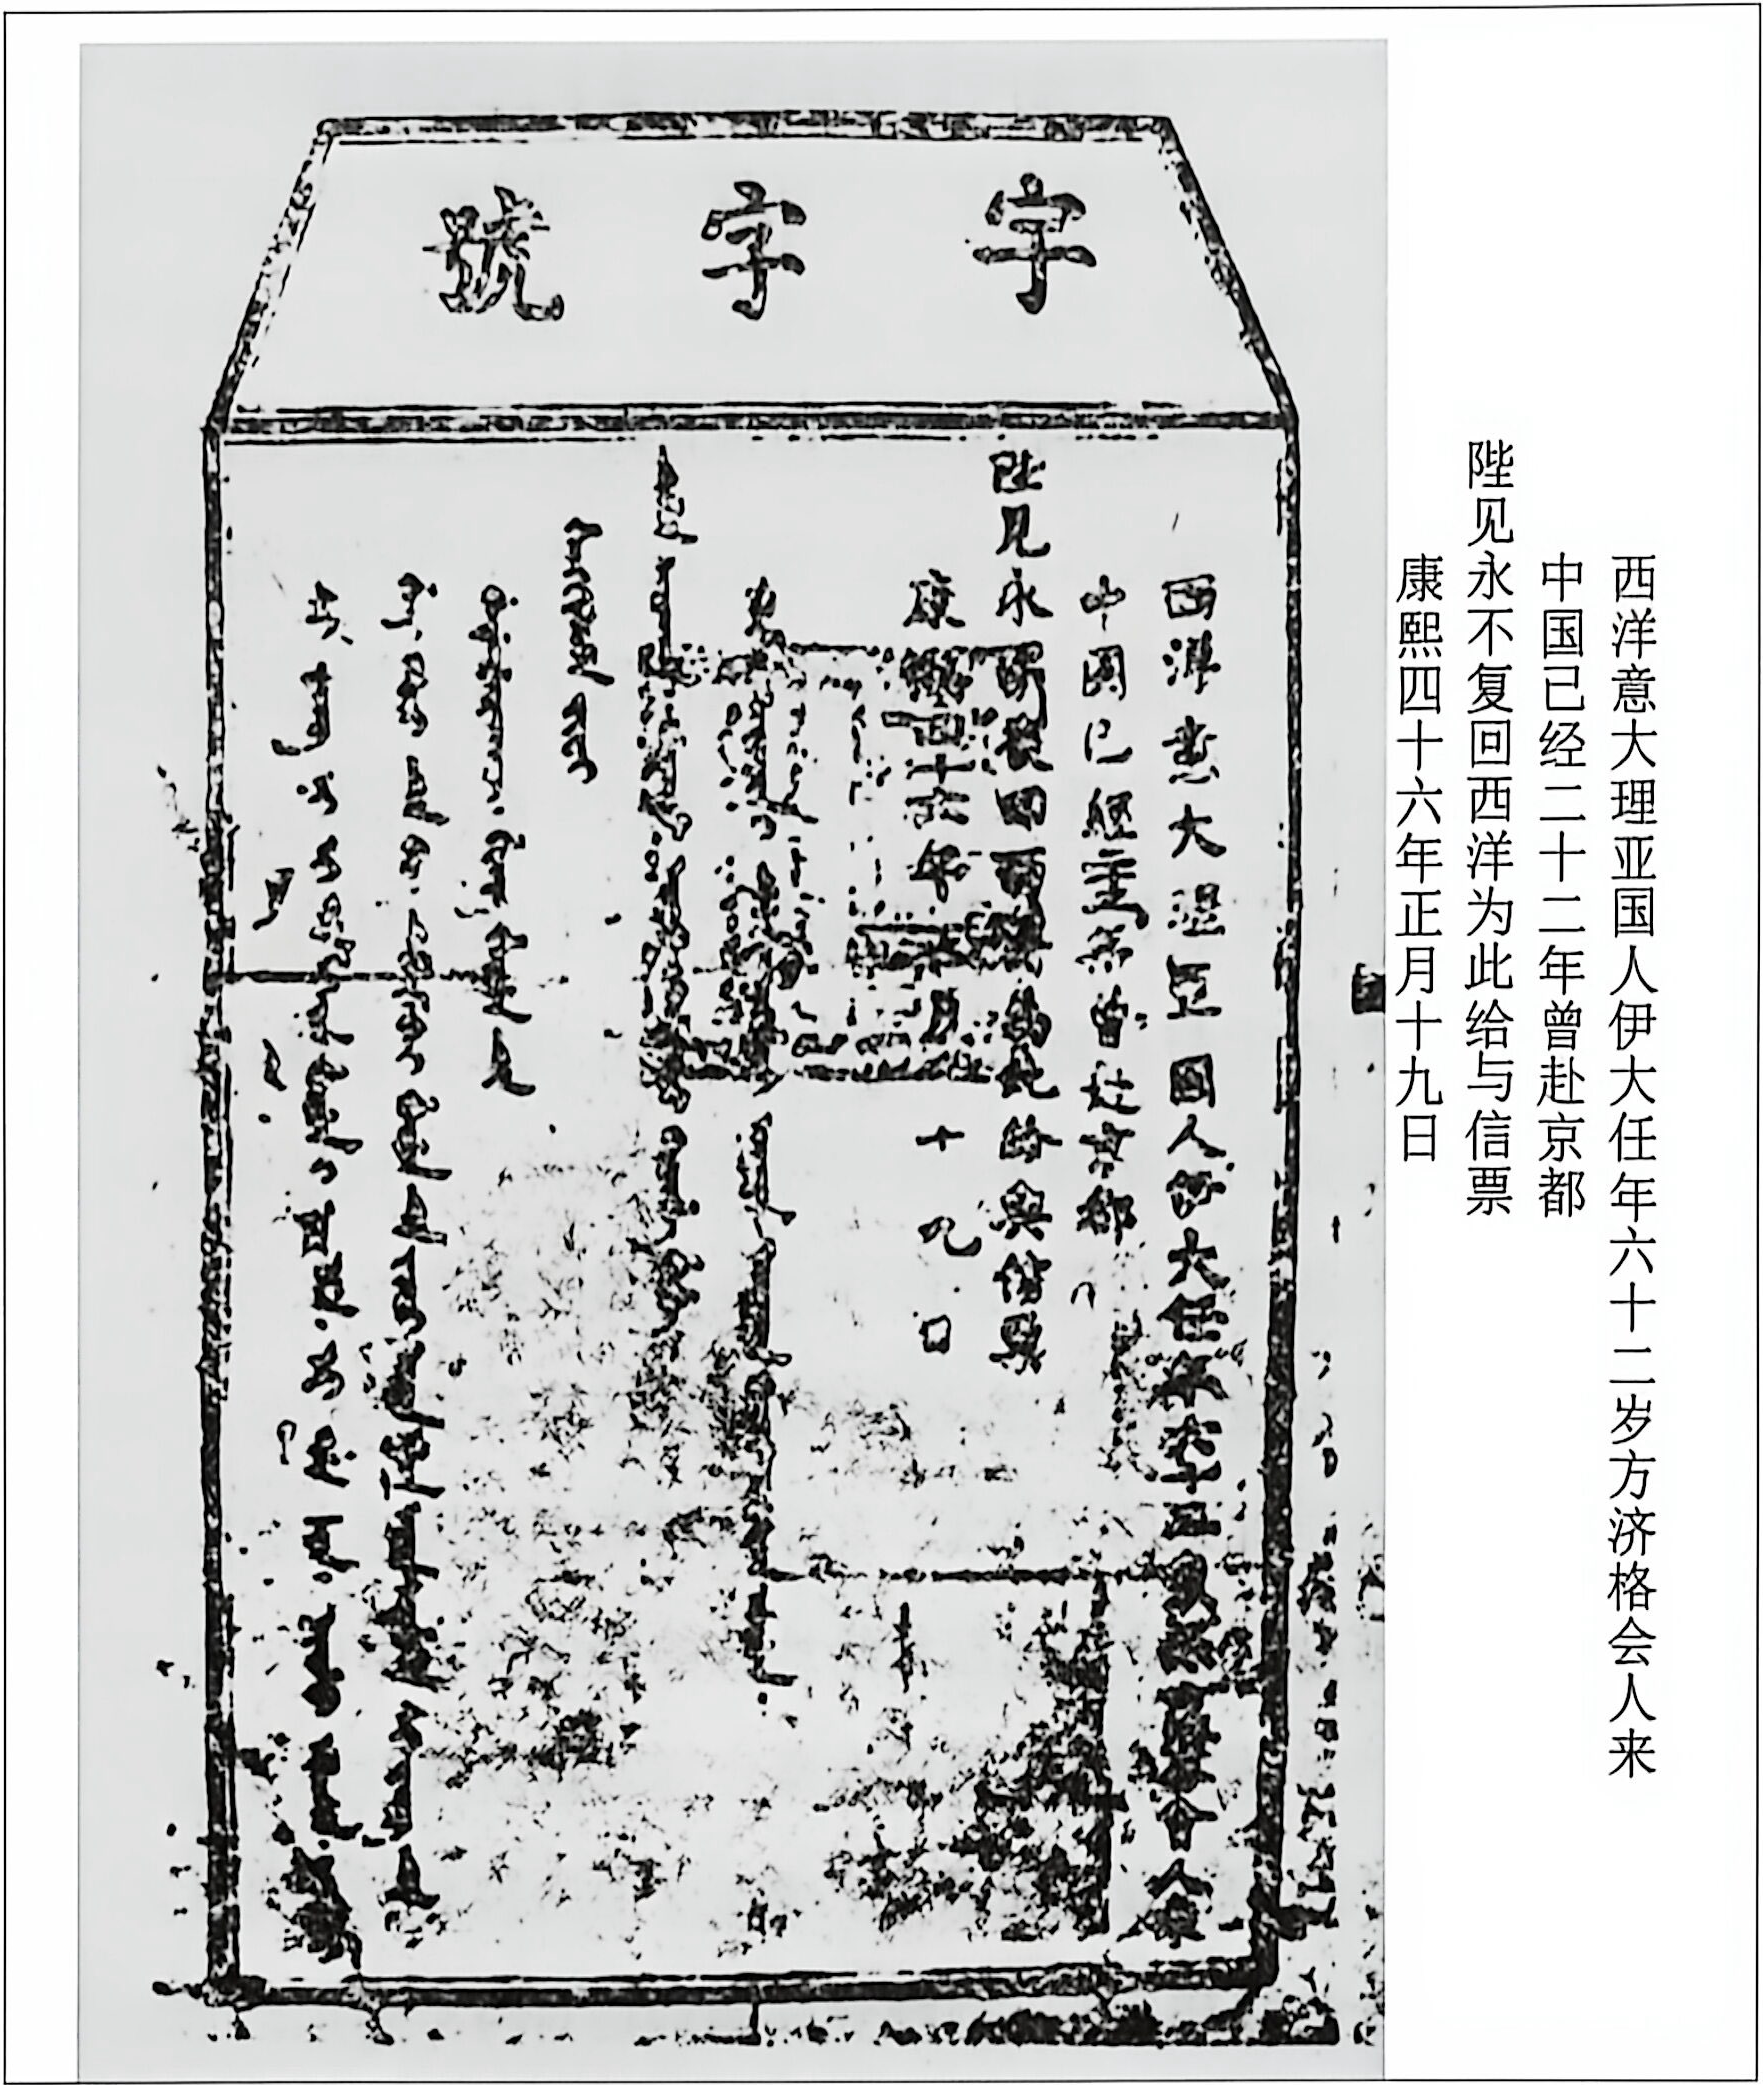
\includegraphics[width=\linewidth,height=.76\textheight,keepaspectratio]{assets/figures/missionary-permit.png}
\caption*{图4.1\quad 内务府发于传教士的印票}
\BookFloatNotes{图片来源：鞠德源，《清宫廷画家郎世宁年谱》，34。}
\end{figure}%
礼部发放的度牒等官文是不一样的。当时在北京的德国传教士纪理%
安（1655—1720）在用拉丁文发回欧洲的记录中还专门对比过：%
\par
% 原书页码：127；段落
{\bookkai 那些说我们与和尚地位差不多的说法是不对的。和尚受官僚机构}%
{\bookkai 以及地方官的管辖。但我们拿的印票，不受制于任何官僚机构。而且}%
{\bookkai 就像赫世亨（康熙身边的包衣奴才）所说的那样，官员们看到我们的}%
{\bookkai 票后都会礼让三分。这些票都是皇上亲自发放的，又称“龙票”，上}%
{\bookkai 面有龙的标志，外加内务府总管的印。这样一来，有这个票的人就不}%
{\bookkai 受普通官员的管辖了。}%
\par
% 原书页码：127；段落
{\bookkai 而且，欧洲人拿到的这个票是在皇帝御前发放的。这在中国来说}%
{\bookkai 是最高的待遇，象征着一种特别的恩宠。当然，这个票也不能拿出去}%
{\bookkai 胡乱使用，小心谨慎也是必不可少的。\NoteRef{4}{32}}%
\par
% 原书页码：127；段落
上面纪理安用拉丁文写给欧洲人看的文字，当然有在父老乡亲面前炫%
耀地位的意思。但了解大清官僚运作机制以后，就知道他说的是真的。%
内务府的人，在地方上确实享有特殊待遇，他们确实不受地方官直接%
管辖。内务府的人如果在地方上犯了事，地方官员要知会内务府，由%
内务府来处理，这种法律上的特权，就是纪理安所谓“不受制于任何%
官僚机构”的意思。而且地方官员都知道传教士是内务府的人，也确%
实对他们礼让三分，或说是敬而远之，因为最让地方官员忌惮的是内%
务府的人有和皇帝的联系渠道。举个例子，在真定府（治所在今河北%
正定县），传教士派去收地租的人和租户因为纠纷打架。注意，只是%
打架，并没有伤亡。这样鸡毛蒜皮的地方事件康熙竟然知道了，还写%
了专门的谕旨给直隶巡抚赵弘燮，谕旨是这样写的：%
\par
% 原书页码：128；段落
{\bookkai 近日闻得京中西洋人说，真定府堂内有票西洋人偶有比此争地，}%
{\bookkai 以致生祸授打等语，未知虚实；但西洋人到中国将三百年，未见不好}%
{\bookkai 处。若事无大关，从宽亦可。尔细查缘由情形，写折奏闻。\NoteRef{4}{33}}%
\par
% 原书页码：128–129；段落（跨页续段）
收到这封谕旨时，赵弘燮根本没听说过这事，地方上没有向他汇报%
过。站在直隶巡抚赵弘燮的角度，他接到谕旨后，会从中看到什么，%
想到什么？第一，康熙专门在西洋人前面加了“有票”二字，也就%
是告诉巡抚，这不是普通西洋人，是拿着康熙印票的西洋人。康熙%
的潜台词是，这些洋人是我府中的人，所以他要过问这件事。第二，%
赵弘燮应该立刻感受到了传教士在京城的能量。一桩地方上的小事，%
他都还不知道，传教士已经让皇帝知道了。第三，他不知道传教士%
在康熙那里是怎么报告这件事的，也不知道康熙迫问这件事的目的%
何在。赵弘燮看完谕旨后应该是有很多想法和顾虑的，这也在他后%
来的汇报中体现了出来。这样一桩小案子他啰啰唆唆地写了很长的%
报告，生怕漏掉了任何细节。从报告来看，事件其实很简单，一个%
当地人把土地典当给了传教士，然后他继续在土地上耕作，这样相%
当于他是土地上的佃户，应该交租。但他拖欠了地租，传教士于是%
派仆人去催缴。在催缴过程中两边从争吵逐渐变成了互相厮打，但%
双方似乎都未有受伤。所以就案情来看，这是一桩再普通不过的地%
方打架斗殴事件。了解全部案情经过后，大概赵弘燮也觉得自己有%
点冤，还专门在报告最后注明这个案子只是地方上的斗殴事件，当%
地已经处理过了，按朝廷规定，这种小案件是不上报朝廷的。这也%
是在向康熙解释，为什么他不知道这个案子，也没有上报过。这个%
% 原书页码：129；图表（图题／表题所在页）
\begin{figure}[tbp]\phantomsection\label{fig-148-0}
\centering
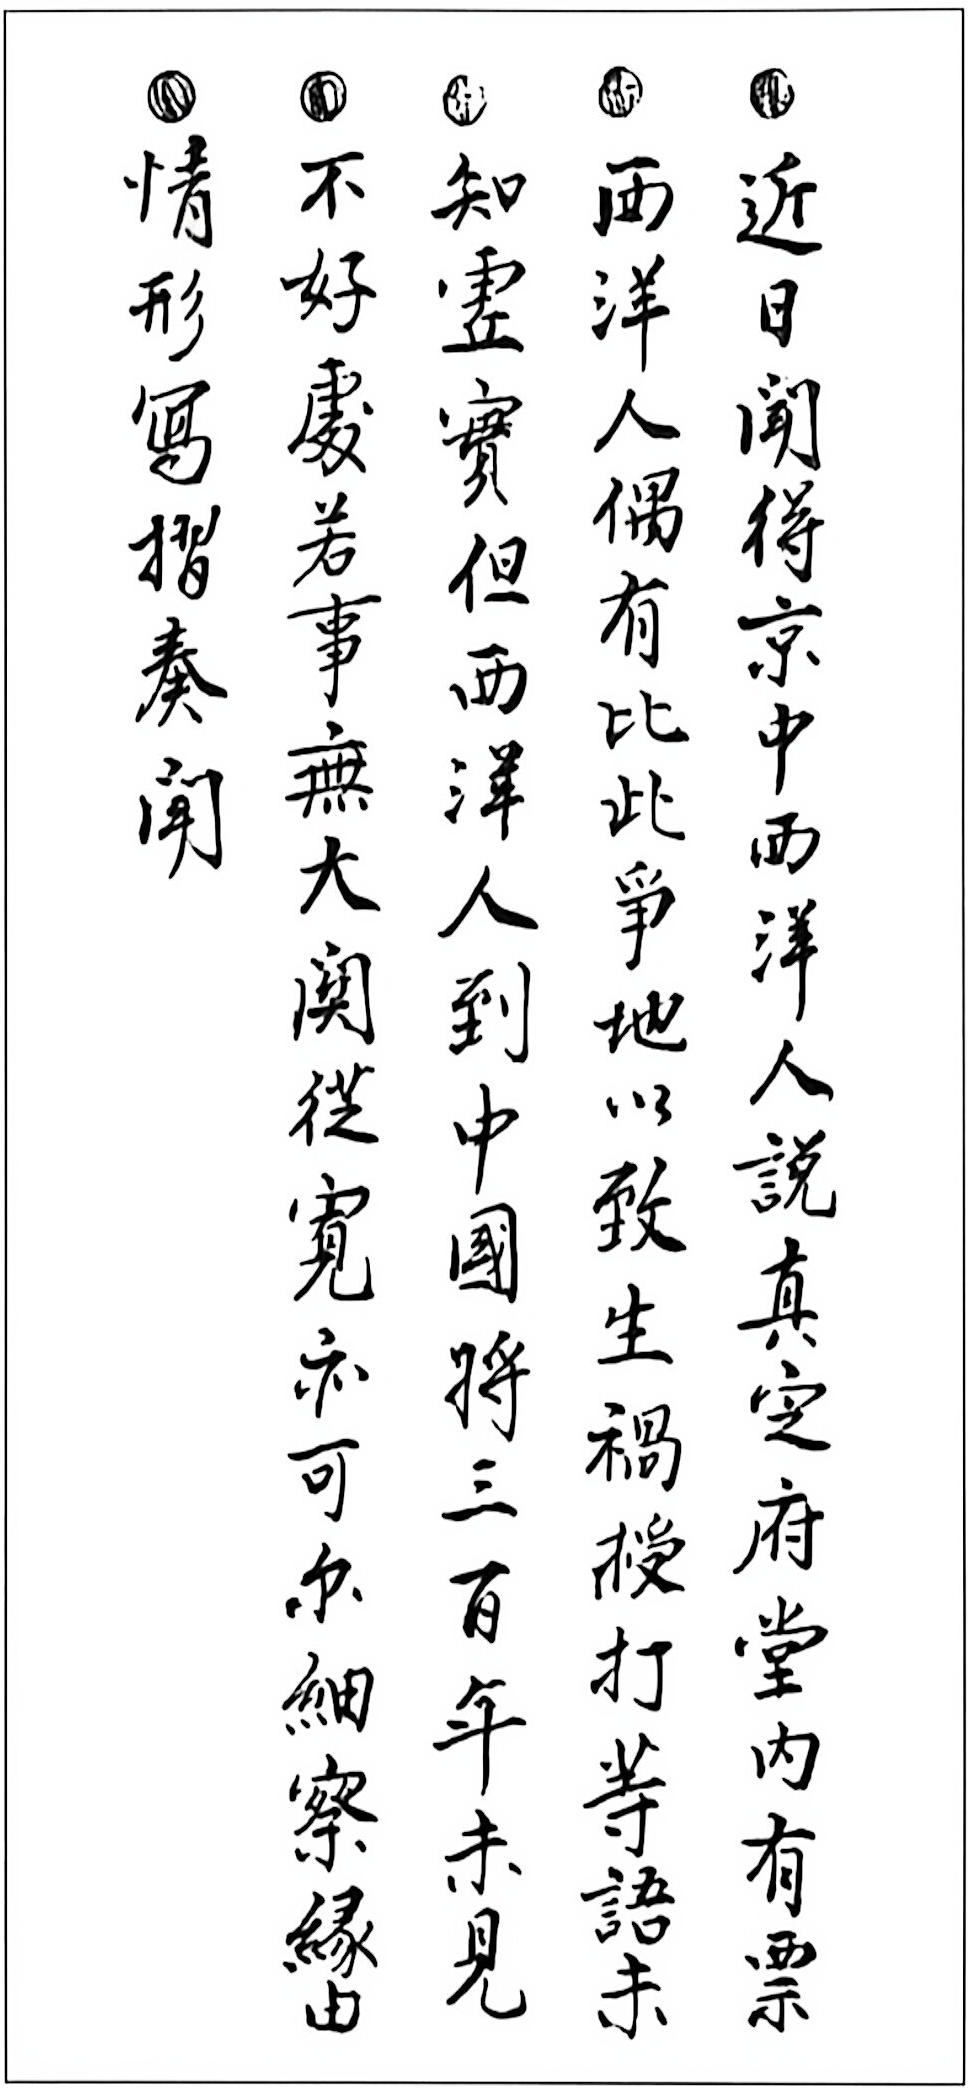
\includegraphics[width=\linewidth,height=.76\textheight,keepaspectratio]{assets/figures/kangxi-fighting-edict.png}
\caption*{图4.2\quad 康熙过问西洋人打架案谕旨}
\BookFloatNotes{图片来源：《康熙朝汉文朱批奏折汇编》，6：108。}
\end{figure}%
案件一来一往似乎只是康熙%
和赵弘燮在对话，但可以想%
象赵弘燮接到康熙谕旨以%
后，一路追查到地方，涉及%
的每一个官员都会很惊讶，%
为什么皇帝会来追查过问这%
种小案子，当然也会马上明%
白这些内务府名下传教士的%
能量。同时，报告中能看出%
赵弘燮也完全领会了康熙谕%
旨中偏袒传教士的意思，因%
为康熙在谕旨中已经明写%
了，尽管他“未知虚实”，%
还是评点了一句“但西洋人%
到中国将三百年，未见不好%
处”。这个“但”字相当于%
已经给案子定调了。身为直%
隶巡抚的赵弘燮不可能看不%
出这个“但”字的意思。所%
以报告最后的结论是康熙圣明，西洋人确实没有什么错。%
\par
% 原书页码：129–130；段落（跨页续段）
其实还没有发票给传教士的时候，康熙就在全国范围内关照传教%
士的生活了。比如1690年，康熙用满文发过私信给山东巡抚，说他%
听说山东有人诬告传教士。山东巡抚接到康熙私信当天，就赶紧派%
人跑遍了省城四处打听，随即上奏康熙，说他打听了一圈，没听说%
有告西洋人的事情。过了四天以后，他终于打听到了，在东昌府茌%
平县（今属山东聊城）下，一位地方居民把房屋卖给了传教士，买%
卖结束后，卖家的一个兄弟出现了，不同意买卖，因而诬告了西洋%
人。案子很小，但康熙这样亲自派人传信过问，着实把山东巡抚吓%
着了。当时通信手段有限，山东巡抚夜以继日加班加点才终于在四%
天之内把案件搞明白。所幸案情简单，涉案问题单一，没惹出大麻烦。%
给康熙的密折中说完案情后，山东巡抚赶紧称赞：“西洋人学问真实，%
断不为不义之事，臣亦知之。”最后，他向康熙认错，说这样的事发%
生了一个多月他都不知道，是他的失职。\NoteRef{4}{34}%
\par
% 原书页码：130–131；段落（跨页续段）
在生活中，康熙对待传教士也确实像一个满人大家族中的主子一%
样，内务府就相当于传教士在中国的娘家。他们想修教堂的时候，会%
写申请到内务府要求拨给土地。\NoteRef{4}{35}传教士需要钱来维修教堂的时候，%
是康熙从他自己的小金库中拿钱出来私下借给他们。\NoteRef{4}{36}他们生病了，%
内科病康熙给他们找中医，骑马摔伤则给他们找满人或者蒙古人医生。%
春节时，康熙按照他打赏自己周围包衣奴才的惯例打赏传教士。传教%
士认为刑部处理与他们相关的案子有不公，康熙就找内务府出面帮他%
们和刑部打招呼。\NoteRef{4}{37}传教士需要马匹出远门，又是内务府给他们开条%
子到兵部去借马（类似于现在使用公家车辆）。\NoteRef{4}{38}传教士修教堂，需要%
木头，内务府又发信给工部，让工部把库存的杉木借给传教士。\NoteRef{4}{39}在%
康熙决定委派耶稣会白晋神父作为他的特使出使欧洲后，教皇使节对%
白晋的身份是否适合出任康熙特使表示了疑问，康熙就直接说白晋是%
他“御前之人”而且是“府中之人”。\NoteRef{4}{40}当康熙得知教皇使节和耶稣会%
神父私下争执时，说了他为什么始终无条件支持耶稣会神父，康熙的%
话很直白：%
\par
% 原书页码：131；段落
{\bookkai 我们就是养一条小狗，也不允许别人欺负。更何况是这些我小时}%
{\bookkai 候就在我周围，跟了我四十五年，我信任的人。\NoteRef{4}{41}}%
\par
% 原书页码：131；段落
这些“人”指的就是北京的耶稣会士。当康熙用“小狗”作比喻，说明%
打狗欺主道理的时候，就是在讲最传统的满人游牧文化。狗和主人之间%
的关系，恰恰是满人中主奴关系最形象的比喻。康熙在杀索额图时就%
说“养犬尚知主恩”，以此表示索额图不知好歹。白晋在一封用满语写%
给康熙的折子中，也跟着满人习惯叫康熙为主子，称康熙为“明主”“大%
主”和“仁主”（详见第五章）。称康熙为“主”（满语Ejen）就是主奴%
关系下的称谓。在传统中国的文臣奏议中都是称“皇上”或者“圣上”。%
“上”是代表皇帝的字眼。称康熙为“主”的，都是康熙的奴才。比如%
在曹寅的奏折中一般不称“圣上”，而是称“圣主”或者“主上”等。%
而康熙也以主子自称，一次给曹寅儿子的回复中，让他把听到的地方上%
的笑话也向他汇报，说让“老主子笑笑也好”。\NoteRef{4}{42}当然，和曹寅父子一样，%
处于主奴关系中的传教士，也享受着各种主奴关系下的特权。%
% 原书页码：131；标题
\subsection{新来的传教士}
\par
% 原书页码：131–132；段落（跨页续段）
鉴于康熙对传教士的关照，和1692年颁布的容教诏书，法国传教%
士认为当时中国有极好的传教机会。李明和白晋人华几年后又回到欧%
洲，撰文著书介绍中国，宣传中国友好的传教氛围。他们介绍中国的%
书都是当时的畅销书，起到的宣传效果也很明显。1703年，仅法国一%
个国家，就有超过三十位神父出发前往中国。\NoteRef{4}{43}南怀仁在世时就很苦%
恼只有很少的传教士来华。为此，他在1678年发信到欧洲鼓励更多%
传教士来华。而在他发信的十年间，整个欧洲总共只有七位神父来到%
中国。\NoteRef{4}{44}%
\par
% 原书页码：132；段落
1699年，白晋从欧洲出发返回中国，有十一位神父和他一同来到%
中国。白晋是康熙的西学老师，在宫里教过康熙好几年，同时他又是%
康熙派回欧洲招募传教士的，算是康熙的钦差。他离开北京的时候，%
已经和广州各级官员打过交道。回到广州的时候，就有水军官员一眼%
认出他来。他在广州上岸后，第一件事就是直接去找两广总督石琳%
（1689—1702年在任），请石琳转告北京，他已经回来了。同时他还请%
石琳帮忙安排，船上有几个人生病了，需要治疗。石琳当然将一切都%
安排周到。据白晋说广州大小官员都来拜访他，持续了三天。白晋乘%
坐的船是法国国王派的船，船长和手下看到白晋受到的礼遇都惊叹不%
已，觉得不可思议。白晋作为一个法国人，一到广州不仅能获得当地%
最高官员接待，而且大小官员还争相来拜访。当然这一切都是因为白%
晋的特殊身份，当地官员知道尽管他没有官衔，但却是天天跟在皇帝%
身边的人，所以大小官员都争相和白晋往来，大献殷勤。\NoteRef{4}{45}%
\par
% 原书页码：132–133；段落（跨页续段）
康熙知道白晋返回后，从内务府里派了一人到广州迎接，而且让%
官员免除了白晋所乘法国船只的各种税费。当时康熙正好在江南南%
巡，便命白晋带着新来的传教士北上，在康熙的龙船上会面。广州官%
员知道一船人要北上见皇上，又热情地为这些新来的洋人送别。最终%
白晋一行在离扬州不远的地方，上船拜见了康熙。白晋说他见到康熙%
时，康熙在窗边，看到他，便问：“身体可好？”完全是老朋友重逢的%
画面。白晋说，当时官员都在，谈话不能深人，大家也比较拘谨。到%
了晚上，他带着新来的传教士再和康熙相见，谈了很久，而且氛围也%
比较随意。\NoteRef{4}{46}%
\par
% 原书页码：133；段落
在船上见面后，康熙让白晋选出五人留在京城听候差遣。这批传%
教士还见了张诚神父。张诚1688年到京后就得到康熙赏识，后来代表%
清朝与俄罗斯谈判《尼布楚条约》，又立了大功。这之后，他就是最%
常出现在康熙身边的传教士之一。康熙三次出击塞外亲征准噶尔，张%
诚都陪同在侧。后来每次南巡，康熙也把张诚带在身边。新来的传教%
士都清楚，他们在这个遥远的异乡，一来就能得到从上至下的照顾和%
恩惠，都是张诚这样侍候在皇帝身边的传教士的功劳。%
\par
% 原书页码：133–134；段落（跨页续段）
1693年，康熙又把内务府一套院子送给了法国传教士，感谢他们%
治好了他的病。当时康熙得了疟疾外加发烧，朝廷内的中医治不好，病%
情一天一天加重。张诚、洪若翰、刘应三位法国神父毛遂自荐为康熙医%
治。他们用金鸡纳树的树皮治好了康熙的病。\NoteRef{4}{47}金鸡纳树原产南美，当%
地人很早就用它来治疗疟疾和发烧，后来耶稣会神父传教到那里，知%
道了这个树皮的妙用，便把它作为一味神药带到世界各地治疗发烧（这%
个树皮治病的有效成分是奎宁）。康熙送的院子在故宫外西北方向不远%
处，由于位置离故宫很近，在当时就属于一流的地段（见图4.3）。这个%
院子后来成了法国传教士的主要住所。院子的位置也在实际生活中缩%
短了法国传教士人宫觐见康熙的距离。第二年，法国传教士得知院子旁%
的一处空地也是内务府的，而且还知道内务府里的太监正在打这块地%
的主意，他们就在太监提交申请之前向内务府申请了这块地，说希望%
在这里修一处教堂。后来康熙权衡以后，把这块地一分为二，给了传教%
士和太监各一半。传教士没有把自已当外人，还跟内务府的太监争“地%
盘”。不过，传教士是很会搞关系的，他们和内务府中的太监相处融洽，%
并没有因为地皮申请影响到双方的关系。\NoteRef{4}{48}%
% 原书页码：134；标题
\subsection{关系网}
\par
% 原书页码：134；段落
新来的传教士去到各个地方传教前，老传教士都会传授他们各种%
注意事项，中国的习俗，与官员打交道的策略，哪些能干哪些不能%
干，等等。不过，到了地方以后，传教士还是会遇到各种预想不到的%
事，这时候京城的传教士就是给他们解决问题的人。比如传教士利圣%
学（Charles de Broissia）到宁波传教，准备在那里修一座教堂。他到宁%
波后，很快就和当地三位地方官搞好了关系，并得到三位官员默许，%
着手在宁波新修教堂。教堂还在修建过程中，三位官员陆续调任其他%
地方。新来的地方官对修教堂一事不予支持。利圣学想了各种办法巴%
结新来的官员，并告诉他其他地方也在修教堂，该官员坚持要通报礼%
部，让北京来裁定。官员认为之前的容教诏书虽未禁止建造新的教堂，%
但也并没有允许新建。\NoteRef{4}{49}%
\par
% 原书页码：134–136；段落（跨页续段，中间插图不另起段）
在知道事情捅到了礼部后，张诚和在京的传教士都很担心，如果%
礼部做出禁修教堂的决定，那么以后全国各地传教都会受到影响。张%
诚动用了在京城的关系，在礼部部议之前，私下找到了礼部尚书。好%
在礼部尚书对该案没有什么异议，表示会给出满意结果。几天后，礼%
% 原书页码：135；图表（图题／表题所在页）
\begin{figure}[tbp]\phantomsection\label{fig-154-0}
\centering
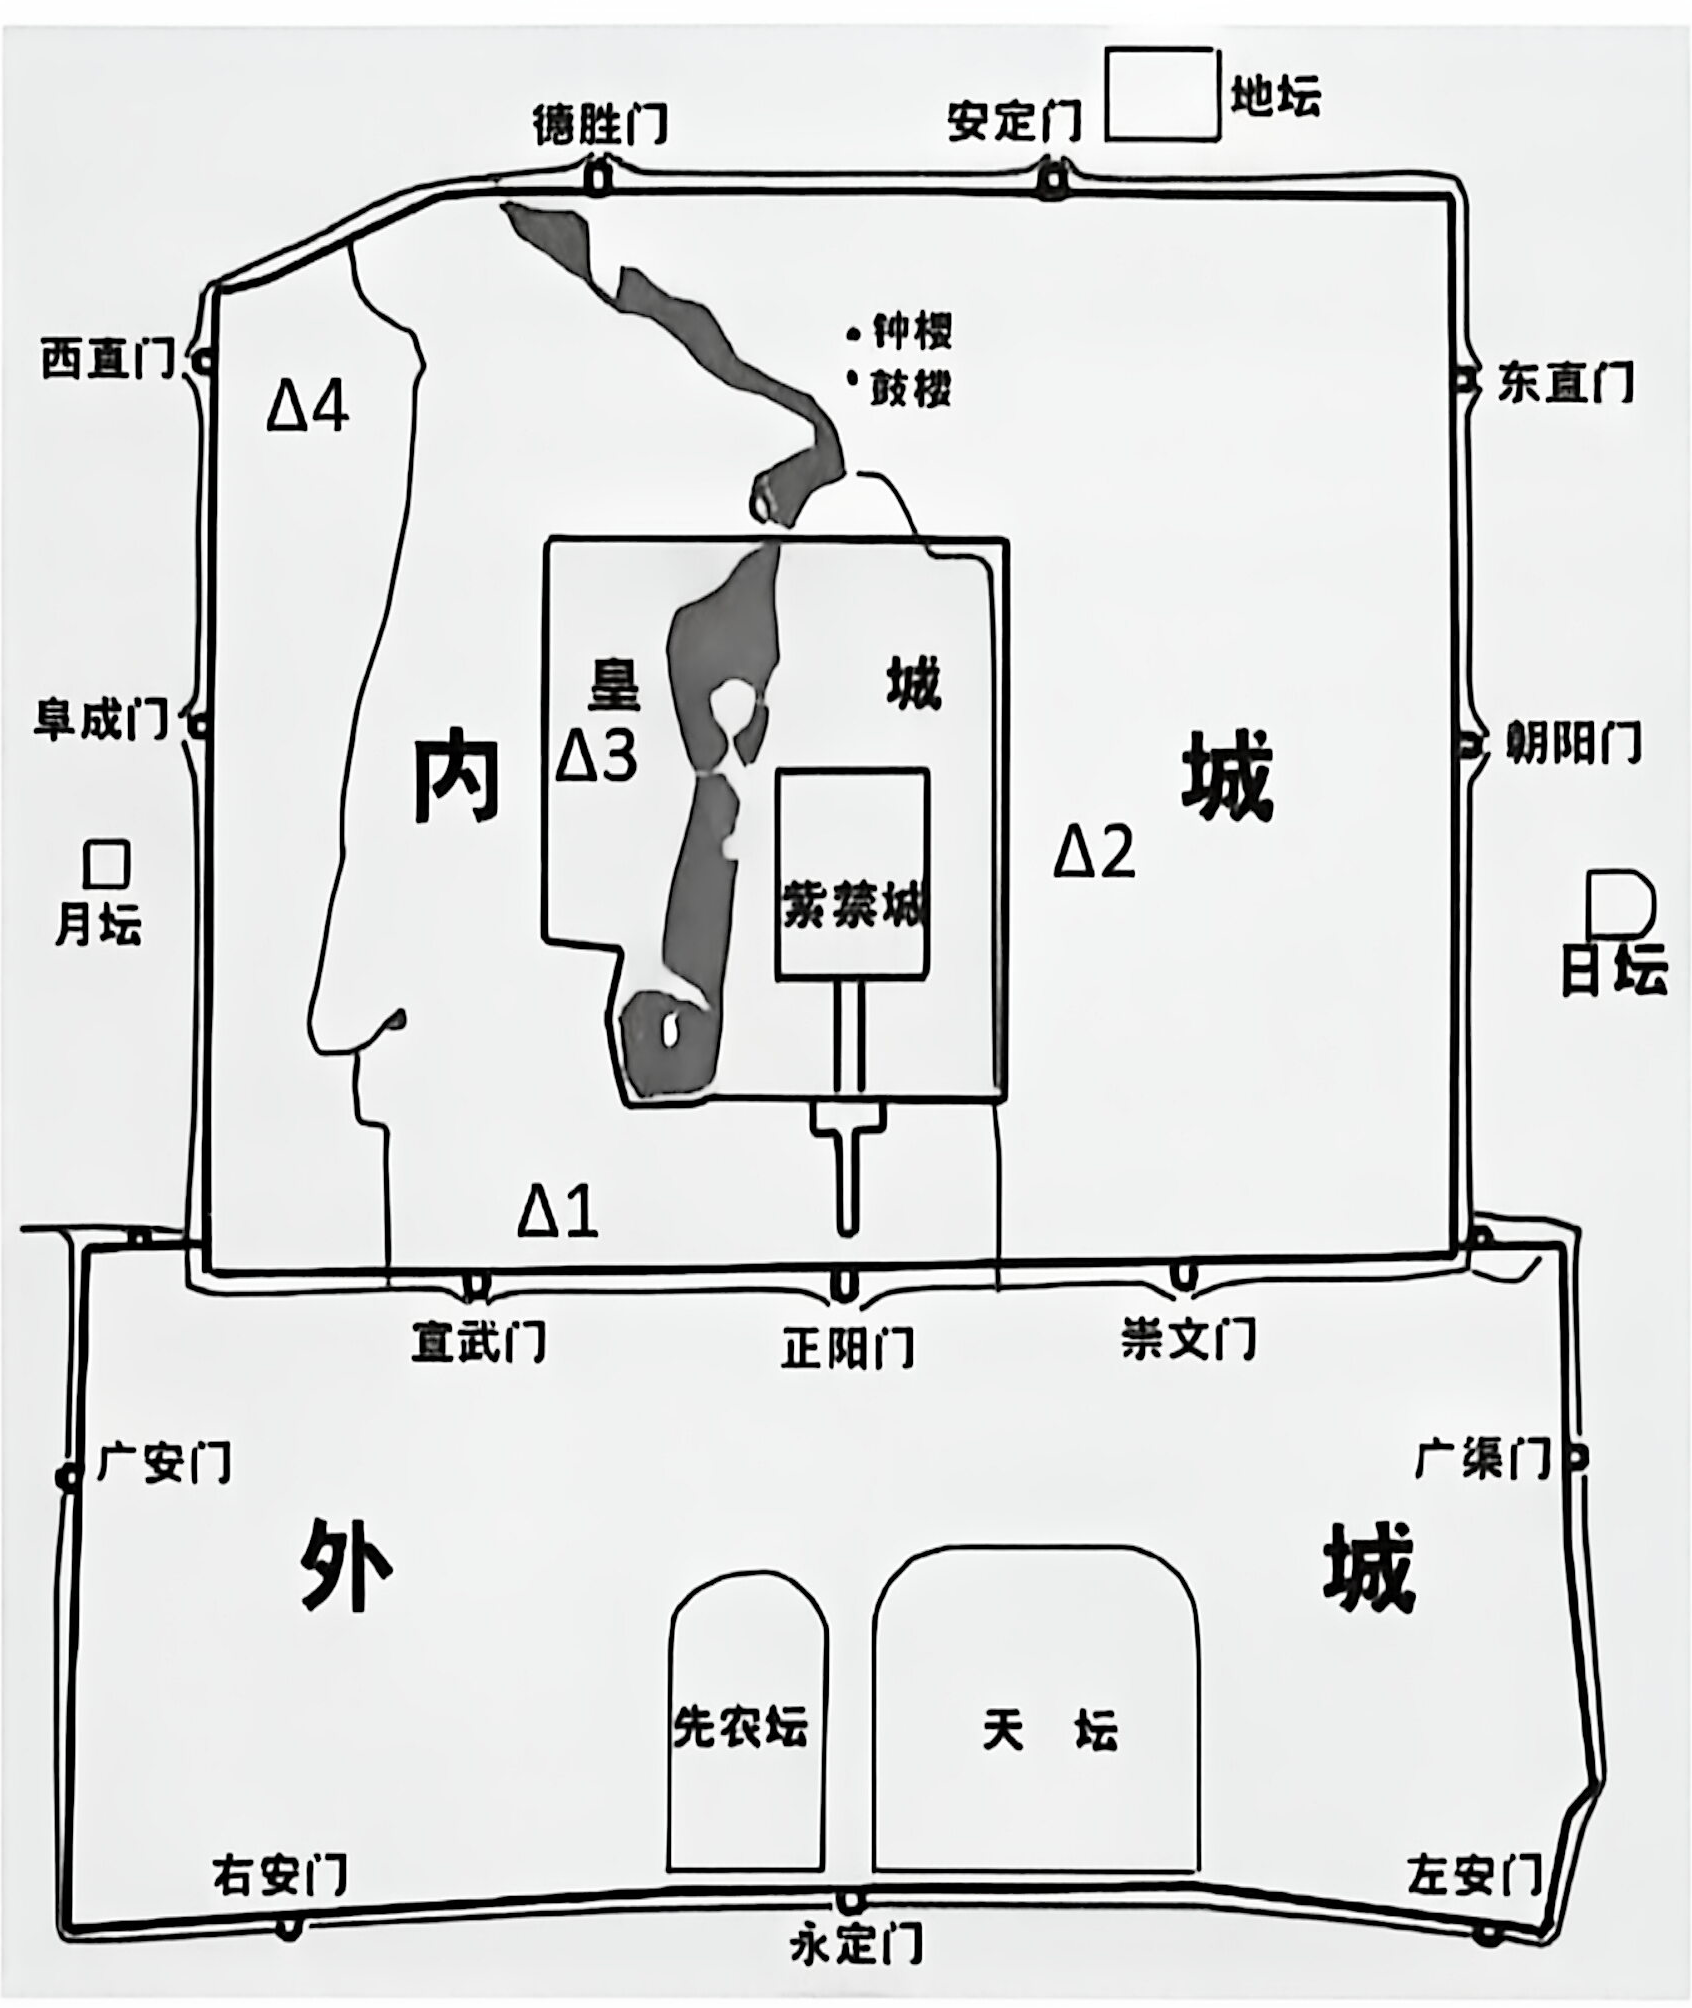
\includegraphics[width=\linewidth,height=.60\textheight,keepaspectratio]{assets/figures/beijing-churches.png}
\caption*{图4.3\quad 清初北京教堂位置图}
\BookFloatNotes{△1：南堂，1605年利玛窦始建，1650年汤若望翻新。又称宣武门天主堂。\par\noindent △2：东堂，1655年利类思和安文思创建。又称圣若瑟堂。\par\noindent △3：北堂，1703年法国传教士创建。又称西什库天主堂。\par\noindent △4：西堂，1723年（雍正元年）德里格创建。又称西直门天主堂。}
\end{figure}%
部给出了允许修建的结论。理由是既然当地能允许修寺庙，那么修教%
堂也应该允许。\NoteRef{4}{50}潜台词是让地方官把教堂当成寺庙一视同仁处理。%
尽管这件事情最后有了满意的结果，京城的传教士还是感觉压力很大，%
通知各地传教士，尽量把地方上的问题就地解决，不要把事情闹到京%
城来。他们认为不可能每一次都有好运气，如果礼部哪次因为某个地%
方案件给出一个不利的结果，那么这个结果会在全国范围都产生负面%
影响。%
\par
% 原书页码：136；段落
由于有这个就地解决问题的方针，洪若翰神父在湖北黄州修教堂%
的计划就只好暂停了。按洪若翰记载，黄州的地方官不仅不同意修教%
堂，还默许道士和地痞在他准备修教堂的地方闹事。洪若翰说他走了%
二百多里去找湖北巡抚。尽管巡抚彬彬有礼地接待了他，但洪若翰%
明显感觉到巡抚在刻意和他保持距离，因为连他带去的小礼品，巡%
抚都不接受。巡抚给出的意见很像托词，说地方要修教堂的话，他%
必须上报礼部。要是北京同意修，他也没有意见。洪若翰在巡抚那里%
无功而返，只好把问题反映给了张诚。张诚通过他京城的关系网，竟%
然找到了巡抚在京城国子监当差的大儿子。传教士并没有详述他们是%
如何打通关节找到这个人的，只是说巡抚大儿子一封家书回去，一切%
都解决了。巡抚收到家书以后，很快找到了当地的耶稣会神父樊西元%
（Jean-Simon Bayard）。传教士的记录中说，巡抚和樊西元聊天中并没有%
谈到修教堂的事，只是谈了谈传教士学习中文等无关的事。不过会谈%
结束后，巡抚就给黄州地方官去了信，信中还附上了康熙的容教诏令。%
地方官接到信后，态度大变，亲自带着礼物找到洪若翰，并在传教士%
住处周围张贴告示，表示允许修建教堂。\NoteRef{4}{51}%
\par
% 原书页码：136–137；段落（跨页续段）
尽管这些传教士是外国人，但在1700年代，他们对中国人情社会%
下各种关系的运作是很老练的。特别需要注意的是，上面两个例子都%
是张诚自己一手搞定的，并没有求助于康熙。比起南怀仁，张诚可以%
说在北京官场已经青出于蓝而胜于蓝了。回想1673年，把一个传教%
士从浙江转去西安这样的芝麻小事，南怀仁都拿不到礼部的批文，还%
需要康熙介人。而此时的张诚已经可以直接私下去找礼部尚书交流了，%
这说明传教士在京城权力圈中已建立了自己的关系网。不过，话又说%
回来，跟权贵交往过密也是双刃剑，遇到政治风波，难免被牵连。后%
来天主教在雍正初年被禁，就和传教士与京城各方权贵交往过密有关。%
这是后话了。%
% 原书页码：137；标题
\subsection{介绍中国}
\par
% 原书页码：137–138；段落（跨页续段）
传教士在朝中有人，同时又有内务府关照，这是地方官都知道%
的。这为传教士在各地的活动提供了方便。当时传教士以及欧洲商%
人走遍了世界各地以后，都认为中华文明是地球上唯一可以和欧洲%
文明媲美的。传教士到中国来传教的同时，带来了西方的科学知识，%
但同时他们也在全方位地学习、考察中国的方方面面。来华的很多%
传教士，自身就是一流的学者。汤若望和南怀仁都是科学素养极高%
的全能型传教士。后来来华的传教士中更是有很多精英。特别是法%
国派来的传教士，这和法国国王路易十四的重视有关。比如第一批%
来华的五位耶稣会传教士白晋、张诚、洪若翰、李明和刘应。其中%
的洪若翰神父，他在法国就是与法国科学院院士一起做研究的。在%
入华航行路上，他就在观测星空，船航行到赤道，他记录下了南半%
球能看到的星空。从他的记录中可以看出，他知道哪些信息有价值，%
哪些是欧洲科学观察急需验证的部分。张诚在欧洲是神父，同时还%
在大学里面教数学。这五位神父在出发之前，法国科学院还给他们%
专门开了各种科学讲座，让他们在数学、天文学、地理学、植物学、%
动物学等众多学科中都有一定的知识储备。\NoteRef{4}{52}这样到中国，如果遇到%
相关发现，才有能力做记录。%
\par
% 原书页码：138；段落
白晋神父其实在数学、天文、技术等方面都是行家，但是他到%
中国后迅速被浩瀚的中国古代典籍吸引。人华后，从一字不识开始%
学习汉语，到博览中国古书，最后深陷在《易经》研究中不能自拔。%
康熙对此还发过脾气，认为白晋不务正业，耽误了他给安排的工作。%
康熙在平定三藩和准噶尔以后，开始丈量国土，绘制全国地图。这%
种工程自然是传教士主导，但这个项目太大，需要大量人手。长城%
外的区域，测量绘制地图，不免风餐露宿，是件苦差事。康熙知道%
白晋当时忙着研究《易经》，但无奈人手不够，还是派他去测绘长城%
部分。结果出去没多久，康熙身边的包衣奴才就报告说，白晋坠马%
摔伤了，在回京的路上。康熙听完很生气，马上意识到这是白晋在%
找借口返回京城。康熙还察觉到，打报告的包衣奴才在帮白晋打圆%
场，便反问道，要真是坠马，就该在坠马的地方养伤，养好了继续%
勘测。这坠马后就回京是什么意思？\NoteRef{4}{53}%
\par
% 原书页码：138–139；段落（跨页续段）
被《易经》吸引的还有法国耶稣会傅圣泽神父。傅圣泽神父是%
1699年人华的，他最初在福建、江西一带传教。傅圣泽深爱中国古代%
经典，其中最让他痴迷的是老子的《道德经》和儒家六经之一的《易%
经》。他钻研《易经》的角度很独特，认为《易经》中的卦象和《圣%
经·旧约》中的一些图像是相通的。他的学问大，在中国传教士内部%
都是公认的。后来有传教士向康熙推荐傅圣泽，康熙便把他召到了北%
京。但傅圣泽对出入宫廷没有兴趣，大约认为这会影响他的研究。他%
几次给康熙的回复都是他水平有限，有很多不懂。但实际他到北京后，%
一直专心研究中国古代典籍，同时忙着在当时北京琉璃厂附近的旧书%
市场淘中国古书。他在中国待了二十年。在1720年返回欧洲时，他购%
买了一千余册中国经典运回欧洲去。回欧洲后不久，便被教皇任命为%
主教。傅圣泽本来就是富家子弟出身，去中国前他在哲学、神学和数%
学方面的造诣已经在法国有名气了。现在他又到中国学了二十年的中%
国经典，又把这些经典带回欧洲翻译，对当时的欧洲学者来说，大约%
相当于我们理解中“唐僧取得真经归来”的感觉。法国当时的大师如%
伏尔泰和卢梭都数次找到傅圣泽当面请教中国方面的问题，以及他对%
很多哲学问题的见解。傅圣泽把中国古代主要的经典都带回了法国，%
开启了法国的汉学研究进程，以至于后来两百年，法国在汉学研究领%
域都是欧洲的翘楚。%
\par
% 原书页码：139–140；段落（跨页续段）
当时中国在世界上最著名的物品无疑是瓷器。在江西传教的法%
国传教士殷弘绪（François Xavier d'Entrecolles，1664—1741）详细记%
录了景德镇烧瓷工艺，1712和1720年他写了两份报告发回欧洲。除%
了自己的观察外，他还从当地人那里得到许多烧制瓷器的关键步骤%
信息。他的报告发回欧洲后，很快被翻译成各种欧洲语言。英国和%
德国当时新建的陶瓷作坊，都得益于殷弘绪神父的报告。当时景德%
镇的师傅对景德镇工艺很有信心，不担心技术外传，他们跟殷弘绪%
神父讲，就是景德镇的熟练工人，换到福建去烧瓷，烧出来的成品%
都要差一截。当时的解释是，景德镇陶瓷的核心是当地的土。这个%
原材料其他地方没有。殷弘绪还介绍说，由于火候控制的原因，整%
窑瓷器全部报废的事经常发生。他说每一个发财的老板背后，都有%
“百名破产者”。这也跟欧洲人解释了为什么中国产的瓷器会那么贵，%
是当时的奢侈品。\NoteRef{4}{54}殷弘绪神父在报告中还特别惊叹于景德镇的治%
安，称当地有三千座瓷窑，人口稠密，而且每天往来商船不断，但%
神奇的是当地只有一位朝廷官员。治安靠商户选出来的地保负责照%
看。作为一个走过世界很多地方的欧洲人，他称景德镇的“治安制%
度很令人钦佩”\NoteRef{4}{55}。殷弘绪神父当时能在饶州和景德镇往来自由，得益%
于各级官府的保护。他在当地的教堂经常还会有官员来拜访。景德%
镇由于进出口瓷器，洋人的商船常到江西来。康熙1708年废太子后，%
经常心慌心悸，在北京传教士介绍下，他喝了少量西洋葡萄酒后症%
状有所改善。为此他晓谕江西巡抚，在来往西洋人那里收集葡萄酒。%
而在饶州（景德镇是当时饶州府下面的一个镇）传教的殷弘绪自然%
也就得到江西巡抚的特别关照。%
\par
% 原书页码：140–141；段落（跨页续段）
康熙在传教士的推荐下使用了一些西医的疗法，同时康熙也派中%
医大夫给传教士治病。传教士在中国见识过中医的疗效，包括针灸。%
传教士到世界各地传教，医疗都是他们的强项，也就是说他们可以通%
过治病来接触和感化信徒。但中国是个例外，尽管西医在某些病的治%
疗上有特色，但是对于大部分的病他们承认是不如中医的。这也是为%
什么传教士是用天文历算而不是医学来进入中国的原因。人都有生老%
病死，传教士也不例外。从第一批传教士明代人华开始，他们很快就%
发现中医在很多病的防治上都有独特思路和疗效。最早系统介绍中医%
和中药的传教士是邓玉函（Johann Schreck，1576—1630）。邓玉函万%
历年间人华，是明清时期所有来华传教士中在欧洲科学界地位最高的%
一位。他年轻时是现代代数创始人韦达的助手，后来是伽利略的学生。%
他早年游学欧洲，在欧洲科学界有一流的关系网。后来他要加入教会，%
伽利略很生气，跟他断绝了往来。到中国后，他被安排去做天文测%
算。当时中国教会需要准确预测日食来显示西方科技的发达，邓玉函%
就发信回欧洲询问天文测算问题。而为他答疑的，是大名鼎鼎的开普%
勒。后来传教士能够很精确地进行日食预测，用的就是开普勒的方法。%
邓玉函在欧洲的本业是植物学和医学。到了中国，遇上中医和中药，%
可以说为他打开了一个崭新的世界。不过可惜的是，在人华十年后%
（1630年），他在一次中药实验中，不幸中毒身亡了。他对中药、把脉、%
针灸都有研究。来华的传教士都希望破解中医治病的原理，他们认为%
中医最神奇的是发现人的脉搏和身体内部运作的关联。古希腊-罗马%
时期西方医学第二号传奇人物盖伦（Aelius Galenus，约 129—216。一%
号人物是现代西医入行誓言的作者希波克拉底）就通过把脉诊病，开%
创了西方的脉学。追随南明朝廷的波兰传教士卜弥格认识到中国的脉%
诊是三维的，医生把脉有按压，以此来感觉脉搏的轻重强弱快慢。他%
把明代成书的《图注脉诀辨真》（一部图文结合便于学习晋代王叔和%
《脉经》的书）翻译成了拉丁文，后来一位荷兰医生把他的翻译收入到%
一本医学方面的综合书籍里。\NoteRef{4}{56}这本书在欧洲多个国家引起了科学家%
的注意。后来的传教士也一直在添补脉学相关的内容。追随南明朝廷%
后来又被孔有德招降的谢务禄神父、第一批来华法国传教士中的李明%
以及1655年荷兰的人华使团，都对脉学有过进一步观察和报告。\NoteRef{4}{57}后%
来西方哮喘研究的奠基人约翰·弗洛耶（John Floyer）就在中国《脉经》%
的基础上，写了一部脉学研究著作。%
\par
% 原书页码：142；段落
传教士走遍世界各地，发现当地的特产，就会介绍回欧洲。比如%
前文说到，传教士在南美看到当地人用金鸡纳树皮治疗疟疾和发烧，%
就把这个树皮传回了欧洲，同时也带到了中国。1693年他们就是用%
金鸡纳树皮治好了康熙。\NoteRef{4}{58}传教士还把巧克力饮料从南美带回欧洲，%
后来也带给了康熙，康熙还很喜欢。\NoteRef{4}{59}他们到了中国，当然也会把中%
国的特产介绍回欧洲。中医在使用自然界动植物上，当时是遥遥领先%
于世界的。这就注定了当时传教士在植物、动物方面有写不完的内容。%
明代早期传教士就写过很多书介绍中国的动植物及其使用方法。殷弘%
绪神父就感叹中医对各种植物的研究太深人了，他根本没有时间完全%
翻阅，只能挑一些欧洲常见的植物看看，然后介绍回欧洲。\NoteRef{4}{60}%
\par
% 原书页码：142；段落
康熙年间的传教士凭借内务府的关系，获知并向西方介绍了一%
些名贵的中药。比如现在价格很贵的虫草。法国传教士巴多明记录说%
虫草贵得不可思议，要四两银子才能买一两。而当时朝廷钦天监监正%
一年的俸禄是一百两银子。也就是说一个朝廷大员的年俸也只能买%
二十五两虫草（跟当下作比，2023年的虫草均价为15万—20万元/%
公斤）。可见虫草清初就很贵。巴多明神父说他没有见过虫草的生长%
环境，只知道它生长在川藏地区。他讲到虫草和人参都有滋补的功能，%
区别是人参有些人服用会引起出血。这和现代讲的人参药性强，虫草%
温补的特性是一致的。而且巴多明神父称他能得到虫草，是因为他和%
川陕总督（他没有明写是谁，可能是岳钟琪）有私交。川陕总督进京%
给皇上带了很多虫草，也送了一些给他。巴多明说他当时正好身体虚%
弱，食用虫草后有显著疗效。当时别人给他介绍的食补方法是用虫草%
炖鸭子。\NoteRef{4}{61}这道食补方子今天依然很流行。%
\par
% 原书页码：143；段落
巴多明还讲到了当时欧洲大量从中国进口大黄。大黄是泻药，可%
以治便秘，这点当时欧洲也发现了。巴多明认为欧洲生服大黄的方法%
比较原始，在治病的同时会引起疼痛。巴多明仔细学习记录了中国炮%
制大黄的过程，再介绍给欧洲。经过中国方式加工后的大黄，再加上%
蜂蜜，巴多明说使用效果好，而且还没有副作用。\NoteRef{4}{62}%
\par
% 原书页码：143；段落
巴多明还提到了阿胶，他不仅知道阿胶是用驴皮制作的，还知道%
制作上等阿胶的阿井。按巴多明的解释，阿井里面的水，和一般的水%
确实有区别，这并不是迷信。北宋《梦溪笔谈》以及明代《本草纲目》%
里面也特别提到过制作阿胶的井里的水有特别之处。巴多明说，那口%
井很珍贵，平时官府在井上贴有封条。巴多明同时提到由于上等阿胶%
产量有限，当时全国各地到处都在卖假阿胶。他说他不能确定阿胶是%
否真有很多疗效，但他可以确认阿胶确实在治疗肺病上有疗效，因为%
有几位传教士都亲身验证过。巴多明也是因为宫里的关系，才能接触%
到上等正宗阿胶。他吃过、用过、研究过，说自已闻一闻就能鉴别出%
阿胶的真假。\NoteRef{4}{63}%
\par
% 原书页码：143；段落
巴多明有很高的语言天赋，他1698年人华后，很快就学会了满%
汉双语的听说读写，而且都很地道。他很快就成为经常在康熙身边的%
传教士，并且和朝廷众多官员都有交往。包括雍正朝的宠臣皇十三子、%
年羹尧和隆科多。他历经康熙、雍正和乾隆三朝，一直混迹在北京的%
权贵圈里。后面章节中还有他的故事。%
\par
% 原书页码：143–144；段落（跨页续段）
像巴多明、殷弘绪这样介绍中国方方面面给欧洲的传教士还有很%
多。康熙年间，有上百个传教士来到中国。每一个入华的传教士在欧%
洲都有他的故乡和他入华前所属的教区，那些地方的教友一直在经济%
上、物质上和精神上支持这些传教士，因而这些传教士也有责任向他%
们在欧洲的故人汇报他们在中国的所见所得。这也是为什么有大量%
传教士介绍中国的文字保留在欧洲的原因。同时入华传教士的学养很%
高，他们很注重宗教以外知识的学习，这样他们在很多领域都有观察，%
写出来的东西也很有价值。北京在康熙年间有三座天主教教堂，这是%
入华传教士的中心。这三座教堂都有专门的图书室，有专门空间存放%
教外图书。那里还存放着欧洲寄过来的书，包括当时欧洲的科学发现，%
同时还有在北京购买的汉文书和满文书。在康熙末年，有朝鲜使团参%
观过北京的教堂，他们声称教堂里藏书超过万册。\NoteRef{4}{64}%
% 原书页码：144；标题
\subsection{中西双向交流}
\par
% 原书页码：144；段落
康熙朝的传教士并不知道百年后欧洲在科学技术方面会有大的突%
破。当时在他们眼中，中国在很多方面都是领先的。所以当时的中西%
交流完全是双向的。欧洲没有而中国有的，他们发现有价值，就传回%
欧洲。比如前文讲到的瓷器烧制技术。同时，欧洲有而中国没有的，%
传教士根据他们传教的需要，就传到中国。比如传教士把欧洲的玻璃%
烧制技术传到了中国。欧洲量产的玻璃在明末传入中国时，中国人最%
初以为是宝石，价格高得离奇。后来法国传教士不仅给中国带来了技%
术，还带来几位欧洲工匠，帮康熙在北京建起了玻璃厂。\NoteRef{4}{65}康熙从南%
方招来学徒，很快北京出产的玻璃制品就可以媲美欧洲，1720年康熙%
赠送给彼得大帝的国礼中就有北京产的玻璃制品。当时的技术传播交%
流是双向的，互通有无。%
\par
% 原书页码：145；段落
当时人的思想中有中外之别，但没有很强的中西之分。特别是对%
实用的东西，有的更多的是有用与没用的区别。就拿中西都有的医学%
来说，康熙和传教士看待医学只有有效与无效的区分或者说适合与不%
适合的区分，并没有现代人有的中西医区分。康熙见识过西药有效后，%
便引进了西药和西医，在他宫里常年储备着多种有用的西药。这些储%
备并不能说明康熙特别看重西医，只是说明他务实。历史中喜欢谈论%
康熙当年被传教士治好了中医都治不好的病，这其实和记录有关，因%
为张诚等法国传教士详细记录了他们治好康熙病的故事。但张诚常年%
被失眠困扰，最后被中医治好了，他就一笔带过。当然也没有哪个中%
医大夫会得意地记录下自己治好失眠的医案。后来的人读到当时中西%
医交流的高光时刻，好像就是西医治好了中医治不了的病，让康熙很%
惊讶。康熙自己和周围的人被中医治好的情况有很多，只是当时人对%
此习以为常，并没有觉得这些是值得记录的事。细读康熙和传教士的%
交往历史就会发现，康熙多次安排医生为传教士治病，可以说每一个%
传教士都接受过中医治疗。%
\par
% 原书页码：145；段落
来华传教士众多，在很多问题上难免观点不同。但就中医和中药%
来说，传教士是一致的赞美惊叹，都是怀着敬意把中医中药介绍回西%
方。欧洲来的人，能在中国找到好的中医看病，都是很高兴的。教皇%
使节来华，路上肠胃出了毛病，进京都是抬入京城的，后来觐见康熙%
时，坐一会儿就很累，身体虚弱，随团的西医一点儿办法都没有。后%
来教皇使节请求康熙的医生给他看病，康熙的中医给他开了一个以槟%
榔为主的方子，把他的肠胃病治好了（方子见图4.4）。%
\par
% 原书页码：145–147；段落（跨页续段）
最后离京的时候，教皇使节已经完全康复，他多次上书康熙表%
% 原书页码：146；图表（图题／表题所在页）
\begin{figure}[tbp]\phantomsection\label{fig-165-0}
\centering
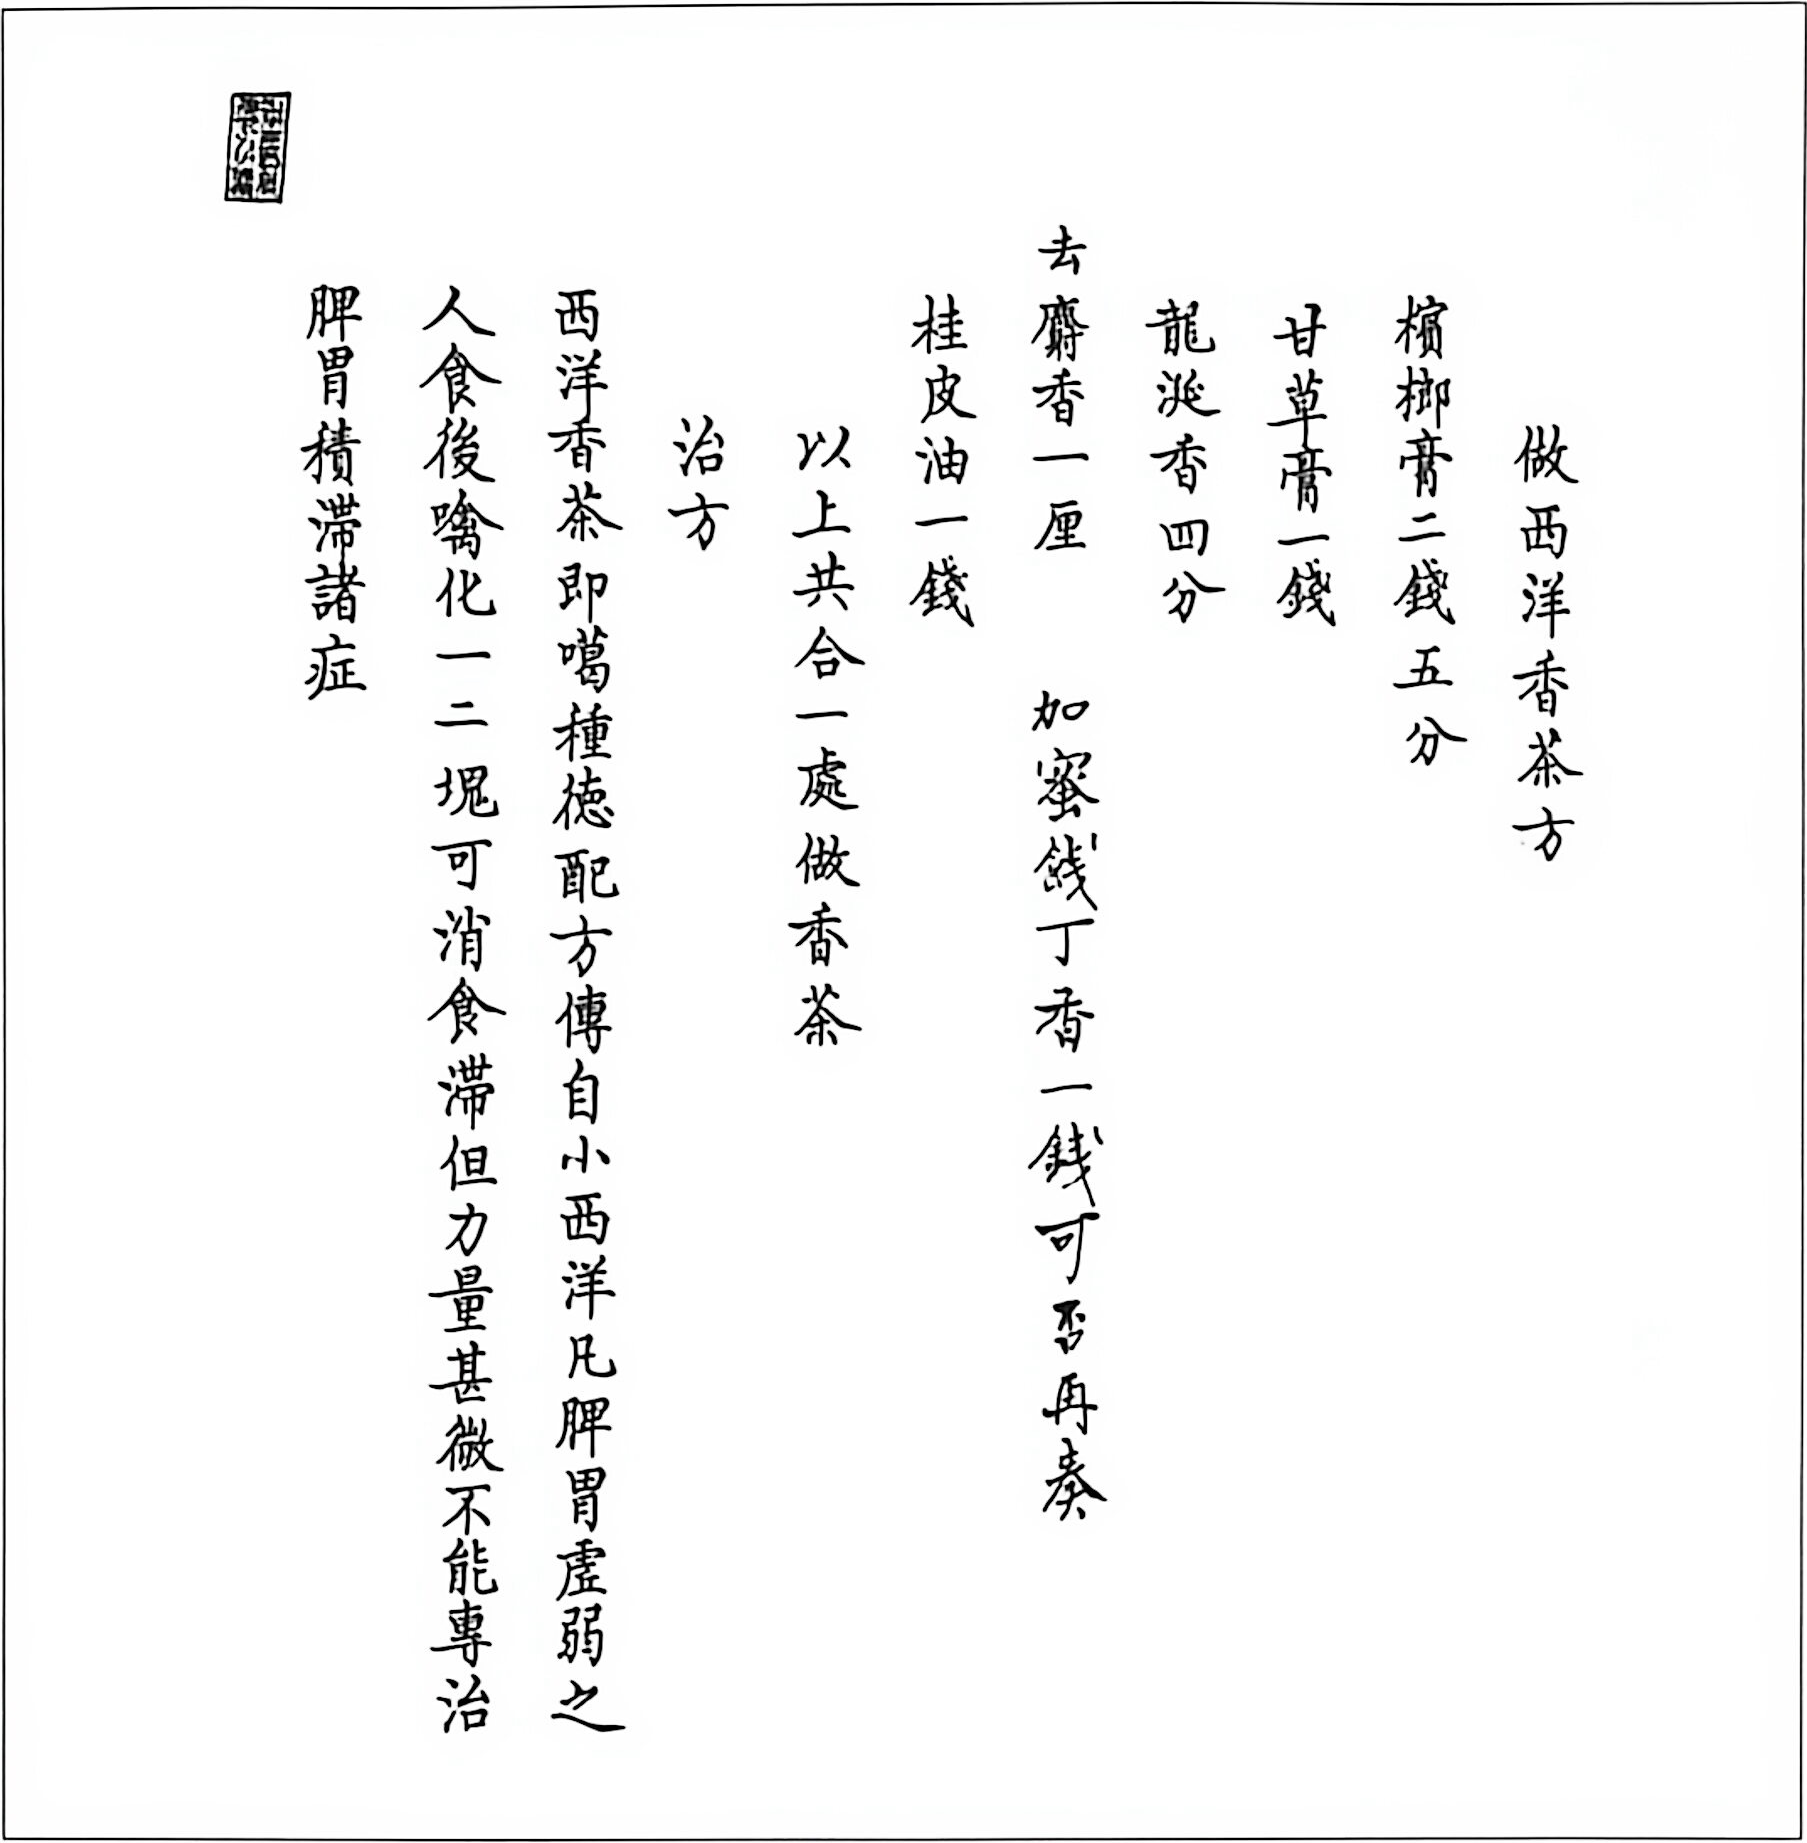
\includegraphics[width=\linewidth,height=.76\textheight,keepaspectratio]{assets/figures/tournon-prescription.png}
\caption*{图4.4\quad 故宫档案藏治疗教皇使节多罗药方}
\BookFloatNotes{图片来源：冯明珠，《坚持与容忍——档案中所见康熙皇帝对中梵关系生变的因应》，182。}
\end{figure}%
示感谢。还有一次，宫里一位西洋画家，大约是画画时间太久，肩%
痛难忍，康熙派医生过去，医生报告说最好的治疗方法是用针灸，%
但是画家很害怕针灸，问康熙该怎么处理。\NoteRef{4}{66}传教士安多病了，康%
熙的御医去看诊，给出的诊断是“中气不足，脾胃虚损，四肢厥冷，%
大便溏稀”等等，开出的是以“附子、干姜、白术”等组成的理中%
汤（是附子理中汤加减）。本来这个病症配搭这个药方是中医的标准%
治法，但有意思的是，御医还加了一句“其病情重大”，可以再用一%
些“圣药德里雅噶”。\NoteRef{4}{67}这个德里雅噶是Theriac的音译，这是古希腊%
开始就有的西药，主要是解毒之用，一直流行到19世纪。\NoteRef{4}{68}传教士%
人华后，把德里雅噶介绍给康熙，并帮助制作出来，存在宫里。康%
熙的御医应该用过这个药，所以才会给安多开出理中汤和德里雅噶%
并用的药方。\NoteRef{4}{69}康熙内廷中备有许多传教士介绍过来的药，这些药当%
时被称为“圣药”，即皇帝才有的药。这些“圣药”不仅宫里人知道，%
康熙私人圈子里的人也都知道。下面一段是康熙在江南的包衣奴才%
李煦去扬州探望病中的曹寅后，向康熙汇报了曹寅的病情，并求“圣%
药”治病的奏折：%
\par
% 原书页码：147；段落
{\bookkai 臣李煦跪奏：江宁织造臣曹寅于六月十六日自江宁来至扬州书局}%
{\bookkai 料理刻工，于七月初一日感受风寒，卧病数日，转而成疟，虽服药调}%
{\bookkai 理，日渐虚弱。……臣随于十五日亲至扬州看视。曹寅向臣言：我病}%
{\bookkai 时来时去，医生用药不能见效，必得主子圣药救我。但我儿子年小，}%
{\bookkai 今若打发他求主子去，目下我身边又无看视之人。求你替我启奏，如}%
{\bookkai 同我自己一样。若得赐药，则尚可起死回生，实蒙天恩再造等语。}%
\par
% 原书页码：147；段落
{\bookkai 臣今在扬看其调理，但病势甚重，臣不敢不据实奏闻，伏乞睿鉴。}%
\par
% 原书页码：147；段落
这里曹寅求的“圣药”就是治疗疟疾的金鸡纳树皮。从下面康熙的回%
复中，可以看出康熙当年被治好后，还仔细研究过传统中医治疗疟疾%
中可能存在的问题，以及金鸡纳这种药的使用注意事项：%
\par
% 原书页码：148；段落
{\bookkai 朱批：尔奏得好。今欲赐治疟疾的药，恐迟延，所以赐驿马星夜赶}%
{\bookkai 去。但疟疾若未转泄痢，还无妨。若转了病，此药用不得。南方庸医，}%
{\bookkai 每每用补济，而伤人者不计其数，须要小心。曹寅元肯吃人参，今得此}%
{\bookkai 病，亦是人参中来的。金鸡拿专治疟疾。用二钱末酒调服。若轻了些，}%
{\bookkai 再吃一服。必要住的。住后或一钱，或八分。连吃二服。可以出根。若}%
% 注70：用户于2026-10-12核对纸书第148页，确认在末句“万嘱！”后、下段之前。
{\bookkai 不是疟疾，此药用不得，须要认真。万嘱，万嘱，万嘱，万嘱！}\NoteRef{4}{70}%
\par
% 原书页码：148；段落
康熙的四个“万嘱”也体现了他对曹寅的关心。在这之前，康熙就知%
道曹寅常吃人参，所以认为曹寅这次病恶化是补药吃错了的缘故。康%
熙的药还是去晚了，曹寅在药送到前去世了。从康熙与他亲近奴才的%
通信中，可看出康熙从实际出发，各种药物并用来治病的实例。在当%
时人眼中，“圣药”是皇帝那里才有的特效药，没有人在乎这药到底%
是中国的还是西洋的。%
\par
% 原书页码：148；段落
大部分传教士人华后，都被中国这片土地以及这里的人和文化所%
吸引，一生都没有再回过欧洲，并安葬在了中国。后来在乾隆朝出名%
的画家郎世宁，其实也是康熙朝人华的。康熙朝传教士愿意人华，跟%
传教士在华的地位分不开。他们是内务府的人，所谓“朝中有人好办%
事”，所以在地方上，他们也能得到各种照顾。这些客观条件，不仅%
方便了他们传教，也促使这些传教士深人地了解中国的方方面面，并%
介绍回欧洲。历史写作和阅读容易时空穿越，但理解历史需要站在当%
时的时空中来理解。在当时的时空中，并没有近代以来产生的所谓西%
方意味着先进和进步这样的观念。当时的中西交流就是相隔很远的两%
个不同文明区域在互通有无、互有启发地平等交流。%
% 原书页码：149；标题
\subsection{小结}
\par
% 原书页码：149；段落
大清的权力分布就是个金字塔，皇帝处于最顶端。当传教士能够%
接近处于塔尖的皇帝和王公大臣，他们就处在一个有利的位置。接近%
高层，接近满人权贵，从而为传教打开方便之门，是清初传教士的策%
略。他们希望以有限的人手撬动大清这个幅员广阔、人口众多的国家，%
最大程度把他们的福音传到中国。南怀仁为如何实现这个基本目标指%
明了方向：就是要像包衣奴才一样与皇帝和满人权贵建立关系。这改%
变了汤若望和之前明代人华传教士希望通过在朝廷做大臣来接触皇帝%
的策略。南怀仁的策略调整反映了他对大清权力结构的深刻了解。大%
清的权力系统有两个：一个是从明代那里继承下来的基于君臣关系的%
朝廷系统；另外一个是满人的内部系统，其中康熙和他的部下讲的是%
主奴关系。%
\par
% 原书页码：149；段落
主奴关系及其衍生出来的派系是理解清初政治的核心。朝廷各部，%
人员流动及升迁任用，表面上看讲的是资历，但真正在后面起关键作%
用的是人员的派系。而这个派系和八旗里面基于主奴关系产生出来的%
派系有关。传教士是看明白了这一点的，所以后来的传教士到北京以%
后，都专注于进人内务府，私下为皇帝服务，争取像满人奴才一样获%
得皇帝的信任。%
\par
% 原书页码：149–150；段落（跨页续段）
维系清初皇亲国戚私人圈子的纽带是信任。这和官僚系统不一样。%
官僚系统通过科举吸收新人，其核心是才能。在私人圈子中，“信任”%
的来源有二：一是来自各种世袭关系，其中最主要的是血缘、姻亲以%
及主奴三种世袭关系；第二个来源是保荐。圈中的人把外面的人推荐%
到圈子中来，这个推荐人其实是用他在圈中已获得的信任来担保新人。%
（见下图）%
\par
% 原书页码：150–151；段落（跨页续段）
传教士能在鳌拜时期就进人康熙的内部圈子，信任来自于主奴关%
系。有了信任，传教士才能被纳人圈子中，开始了和康熙的往来。在%
往来过程中，双方关系变近，传教士就有了特权。这些特权包括可以%
私下见到康熙，有专门和康熙联系的通讯渠道，以及在地方上获得优%
% 原书页码：150；图表（图题／表题所在页）
\begin{figure}[tbp]
\centering
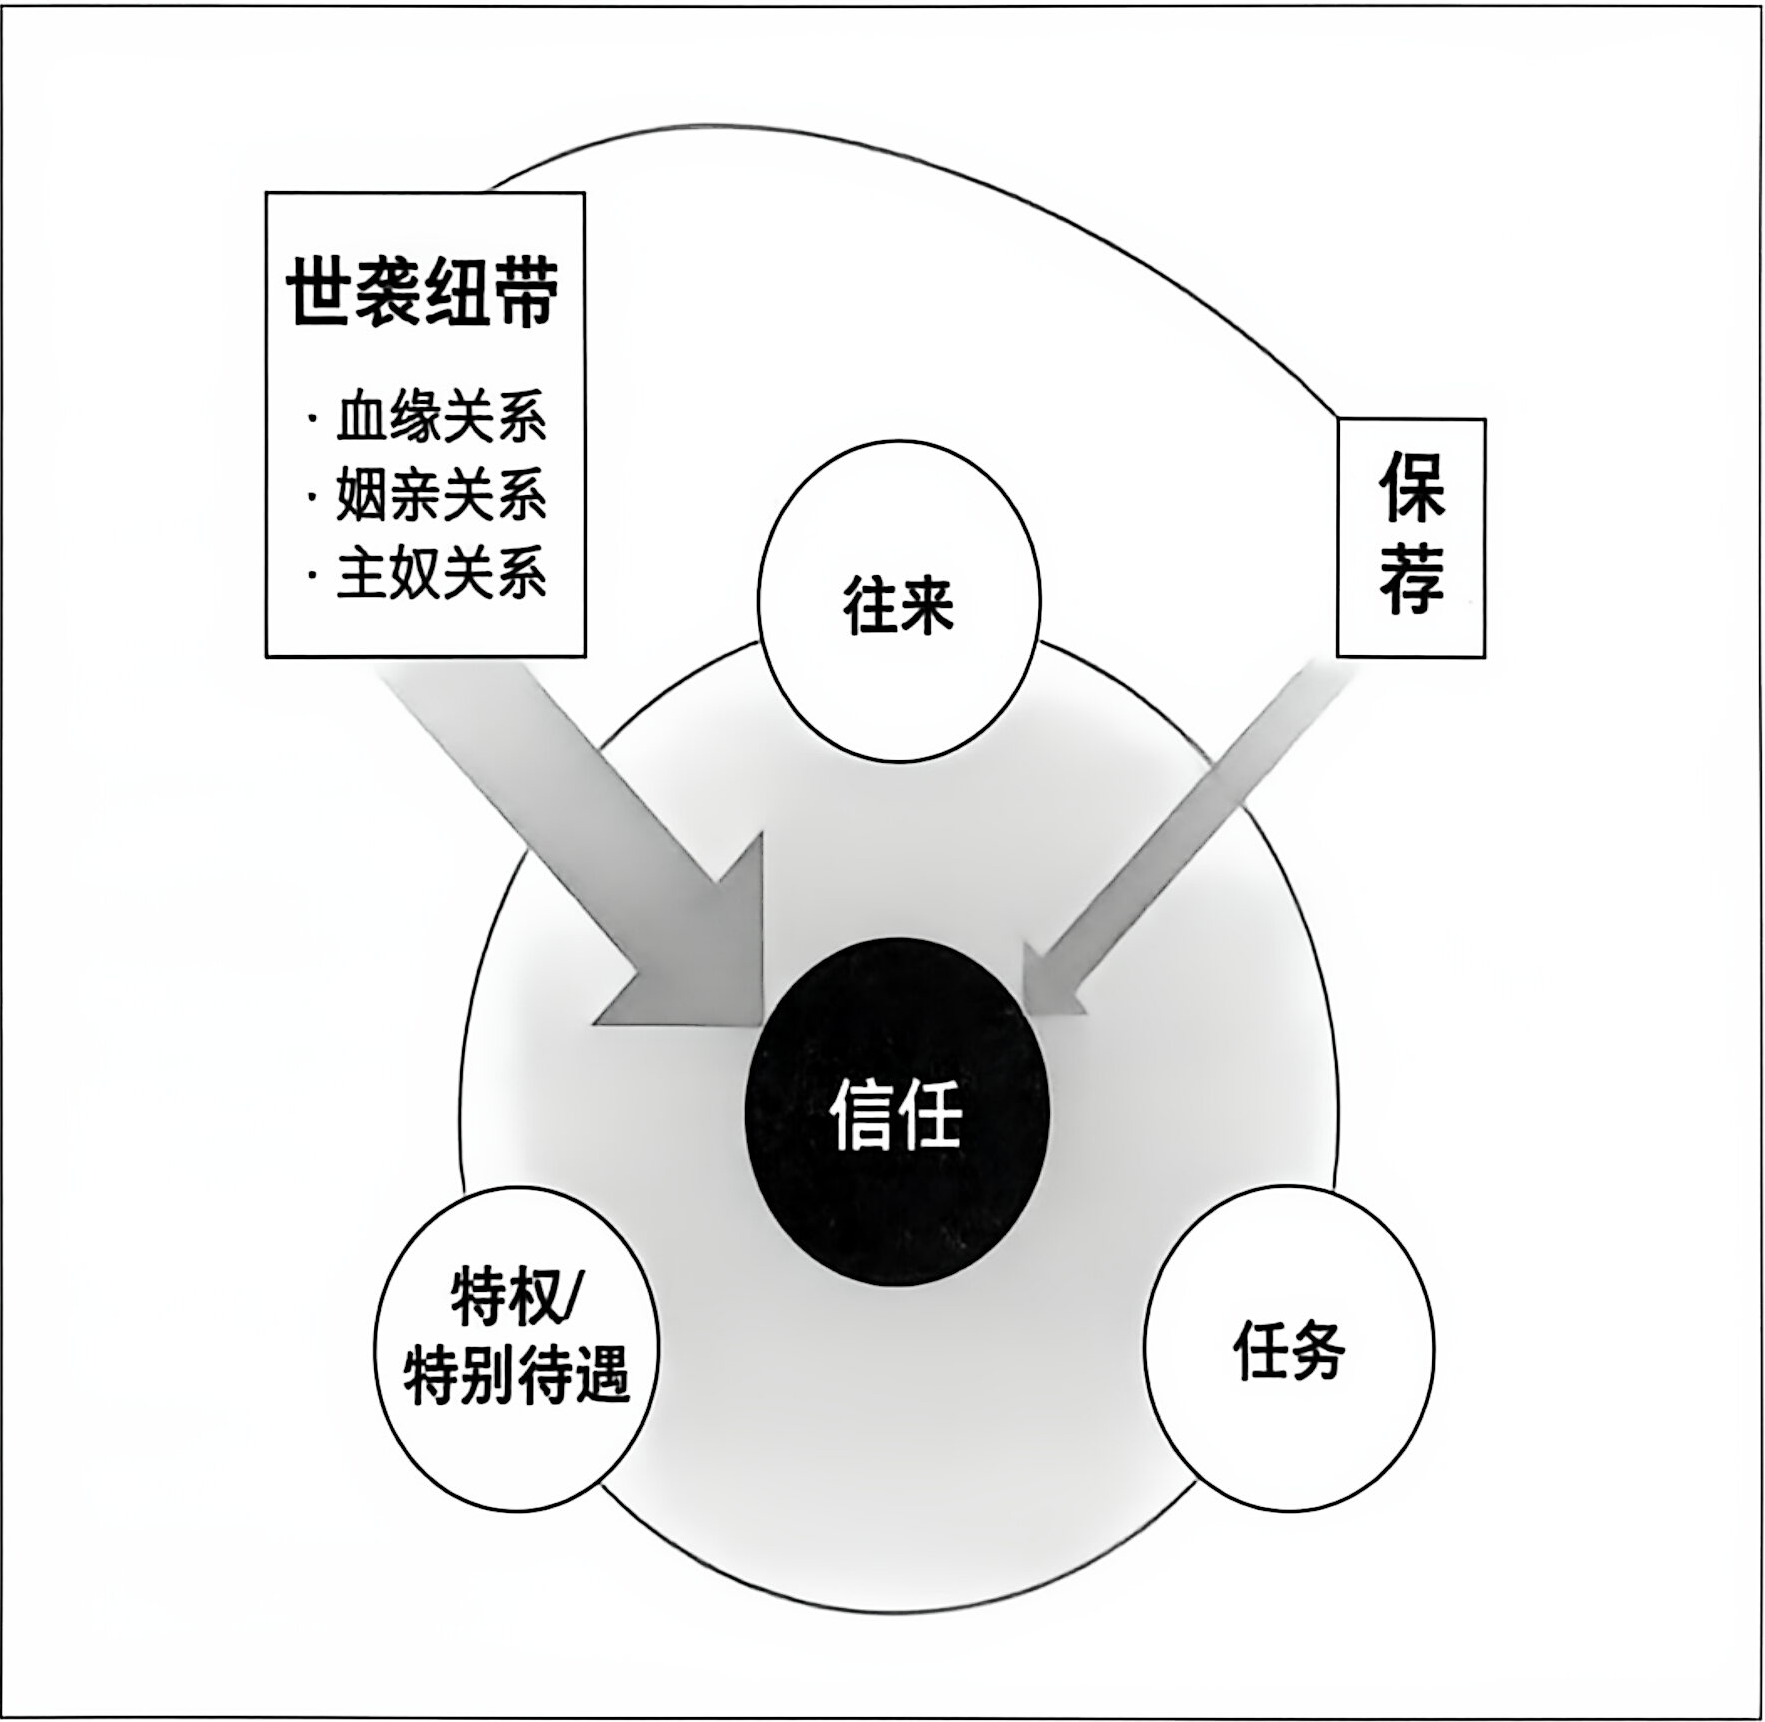
\includegraphics[width=\linewidth,height=.76\textheight,keepaspectratio]{assets/figures/kangxi-private-network.png}
\caption*{康熙私人关系网络运行示意图}
\end{figure}%
待，等等。有了这些特权，也便于传教士完成康熙分配的任务。在完%
成一个个任务的过程中又加强了双方的往来和信任。这就形成了一个%
良性循环。这三个要素的循环在清初以来的私人关系网中随处可见，%
而整个过程中最核心的就是信任。只要信任没有因为某件大事被破坏，%
那么双方关系就会持续。所幸的是，传教士在康熙一朝都没有辜负康%
熙对他们的信任，包括后来教皇派使节到中国来的时候。%
\par
% 原书页码：151；段落
康熙把传教士纳入自已私人圈子，其实也方便他对传教士的管%
理和任用。从皇帝的权力运作方面来讲，大清从明代那里继承下来%
的朝廷制度有很多条条框框。康熙作为皇帝，也必须尊重这些朝廷%
规矩，不能不理会大臣们的意见。容教诏书通过的全过程就很能说%
明问题。当时传教士就在写给欧洲信中解释过：“当皇帝征求大臣们%
的意见时，大臣们根据国法来回答，人们既不能责备他们，也不能%
对他们进行任何非难。”\NoteRef{4}{71}所以，最后康熙解决问题的方法还是派索额%
图去私下活动疏通。由于有朝廷的规章制度在，后来康熙和传教士%
都在有意识地避免把问题送到朝廷的官僚体系下去解决。对于康熙%
来说，绕开朝廷的方法就是把问题变成家事，这样就可以顺理成章%
地让内务府来处理。内务府就是康熙的内府，里面的事就是他的家%
事，自然里面的一切都是康熙一个人说了算，这样他就完全不需要%
考虑朝廷那边的各种成规。康熙如何把“国事”操办成“家事”，这%
就是后面两章的话题。%

\clearpage\markboth{第二部分\quad 红票与中西交往}{第二部分\quad 红票与中西交往}
% 第二部分 红票与中西交往
% 原书页码：无印刷页码；标题
\part{红票与中西交往}

\clearpage\markboth{第五章\quad 教皇使团和康熙派出的洋钦差}{第五章\quad 教皇使团和康熙派出的洋钦差}
% 第五章 教皇使团和康熙派出的洋钦差
% 原书页码：155；标题
\section{教皇使团和康熙派出的洋钦差}
\par
% 原书页码：155；段落
1704年11月20日，教皇克莱孟十一世（ClementXI，1649—%
1721）签署了教内的禁约，禁止天主教徒参与中国传统的礼仪活动。明%
朝末年以来，不同天主教教会，甚至不同的传教士个人，在如何界定一%
些中国传统的仪礼上存在着分歧。比如，中国人在家里供奉死去亲人的%
牌位，在牌位前面上几支香，或者在家里供奉孔子的画像，这些算不算%
天主教教义里不允许的偶像崇拜？中国传统的习俗跟一神论的天主教%
有没有冲突？如果一个中国人皈依了天主教，婚丧嫁娶中哪些中国的%
传统仪礼他可以参与？哪些不能？这一大堆的争议，在天主教内部一%
直都没有定论。这些天主教内部的争论历史上称为中国礼仪之争。在%
中国传教的不同教会对许多问题都各有理解，互相说服不了，只好把%
各自意见发回到罗马教皇那里，让教皇仲裁。简单来说，认为可以允许%
信徒继续参与礼仪活动的一方认为中国的这些仪礼属于世俗层面，没%
有宗教层面的偶像崇拜意味，所以没有必要在教徒中禁止这些仪礼。%
\par
% 原书页码：156；段落
为了说服罗马教廷，耶稣会神父在1700年发了一个装着各种文%
件的大包裹去罗马。这里面包括他们翻译的儒家士大夫的论述，以%
及一篇他们写的并得到康熙认可的分析。作为旁证，他们还特意找%
到住在开封的犹太人，让他们写下了他们眼中的中国仪礼。不过教%
皇没有认同耶稣会神父的论点。为了尽快结束这个争论了半个世纪%
的话题，教皇签署了禁止教徒参与中国礼仪的谕令。不过，由于考%
虑到庞大的中国是很有前景的福音传播地，以及对于欧洲各国的国%
王来说中国在当时世界航海贸易中地位至关重要，教皇特地派了一%
个使团到中国来做沟通。%
\par
% 原书页码：156；段落
在1705年，首位教皇特使多罗到达北京之前，礼仪问题主要在欧%
洲争论。在华耶稣会士知道多罗到来以后，认为这是一个绝好的机会，%
可以在中国给多罗讲解中国礼仪，传达他们的观点。在华耶稣会士懂%
中文，也读了中国各种典籍，理所当然地认为在天主教世界，他们才%
是真正的中国通，他们才有资格解释中国礼仪，而教皇应该接受他们%
的观点。认为中国礼仪中有宗教意味的主要是天主教中多明我会的传%
教士（耶稣会内部也有神父反对中国礼仪）。他们的说法其实也有一%
定道理。比如拜祭孔子，拜祭中当然有尊师重道的意思，但是很多人%
祭孔时也在祈求孔子保佑能考取功名等。在天主教的教义中，他们是%
不能允许信徒对其他偶像祈祷的。还有拜祭祖先牌位这些，其中有没%
有祈求保佑的成分，都是很难说清楚的事。%
\par
% 原书页码：156–157；段落（跨页续段）
康熙也不是完全不知道欧洲在争论中国的礼仪问题。他或多或少%
从身边耶稣会神父那里听到一些风声。1700年，耶稣会神父在准备资%
料解释中国礼仪问题的时候，有一份论述就呈给了康熙过目，还让康%
熙签名支持了他们的观点。不过，康熙并没有把这些争论放在心上，%
也没有关注过。当听说多罗使团人华，他也没有想到过这个使团是来%
处理中国礼仪问题争论的。他最初以为多罗是来调解葡萄牙耶稣会神%
父和法国耶稣会神父之间的内部矛盾的，因为他知道双方有很多家长%
里短扯不清楚的问题。直到多罗人华半年以后，在康熙给多罗饯行那%
天，耶稣会神父才把问题报给康熙，希望康熙出面支持他们的观点，%
要求多罗把他们关于中国礼仪的意见带回到教皇那里。不过耶稣会神%
父把问题捅到康熙那里以后，整个事件走向就改变了。康熙作为大清%
皇帝立马把这个问题当成他自己的事，参与到了争论中去。%
% 原书页码：157；标题
\subsection{康熙和他的江山}
\par
% 原书页码：157；段落
1705年，康熙五十一岁。从铲除鳌拜算起，他已经亲政三十七年。%
作为第二位在京的满人皇帝，康熙先是平定了持续八年的三藩之乱。%
之后他直接掌控了繁华的南方诸省。在平定台湾一年后，也就是1684%
年，康熙第一次南巡。到1705年，他已经五次南下，其间登了泰山，%
拜了孔庙，还祭了大禹陵。康熙用这些象征性的行动在收服中华文人%
士子的心。同时在南巡中，康熙也见识了江南的富足，感受了传统中%
国的人文地理，对他治下的南方有了感性的认识。%
\par
% 原书页码：157–158；段落（跨页续段）
南方平定后，康熙把主要精力放到了北方。除了一直和俄罗斯谈%
判，在1689年签订《尼布楚条约》以外，康熙的主要对手是准噶尔%
汗国的噶尔丹汗（1644—1697）。噶尔丹早年在西藏学佛二十年，在%
学佛修行方面是有造诣的，他的上师是藏传佛教的大德。噶尔丹在他%
哥哥僧格汗被杀后，还俗去当可汗，开始了他的草原征战生涯。噶尔%
丹坐稳了可汗的位置后，趁喀尔喀蒙古内乱之时，侵吞了喀尔喀蒙古%
的土地，势力挑战着清朝在草原上的权威。康熙招降过噶尔丹，但遭%
到了拒绝。%
\par
% 原书页码：158；段落
对于康熙来说，噶尔丹是大清的心腹大患。一来噶尔丹不是只会%
挽弓射雕的普通蒙古部落首领，他是有文化并得到西藏活佛暗中支持%
的可汗。\NoteRef{5}{1}噶尔丹的存在，时刻提醒着康熙当年女真金朝被灭的历史。%
原本被金朝压制的成吉思汗，在统一了蒙古各部后，反过来把金朝给%
灭了。所以康熙不能坐视噶尔丹壮大。但征讨噶尔丹有很多实际困难。%
朝廷上下都反对远征，因为大家都知道，在草原上的噶尔丹骑兵来去%
无踪，可以随时西撤。而大清要远征的话，远距离后勤补给也是很现%
实的问题。不过康熙还是力排众议，决定征讨噶尔丹，而且还是御驾%
亲征。为了彻底消灭噶尔丹，康熙三次亲自出大漠远征，足见他对噶%
尔丹的重视。在1696年第二次远征中，大清同时派出三支大军北上，%
意在包围噶尔丹部队。康熙亲自指挥中路大军，与士兵同吃同住，北%
出一千多公里，穿越戈壁大漠，直接迎战噶尔丹主力。噶尔丹得知康%
熙亲征以后，迅速西撤，不过正好碰上大清左翼大军。噶尔丹仅率几%
十残部逃脱。第二年，噶尔丹在康熙第三次亲征中再次兵败。有传说%
他最后自杀。后世还留传有他生前用藏文写下的诀别诗。诗中的内容%
是希望他的上师能够拯救他，让他有机会转世到能听闻佛法的地方，%
来世有机会研习佛法。%
\par
% 原书页码：158–159；段落（跨页续段）
康熙亲征剿灭噶尔丹后，声名在大漠中远播，使他成为名副其%
实的蒙古各部可汗的可汗。耶稣会神父在康熙三次远征中，都跟随%
在侧。在大漠晴朗的夜空下，耶稣会神父和康熙一起仰望星空，探%
讨学问。他们留下了详细的随军日记，是后世了解康熙远征最详细%
的资料。\NoteRef{5}{2}%
\par
% 原书页码：159；段落
以传统中国的家庭标准来看，1705年的康熙也是很成功的。他%
有十五个儿子，其中九个已成年，都是能文能武、独当一面的角色。%
康熙1696年亲征噶尔丹之时，有六个儿子随他出征。这个时期的康%
熙家庭和睦，后来困扰他的皇子争位之事还未开始。应该说此时的%
康熙家和国强、天下归一、名震四海。就连欧洲的哲学家这时期都%
在读康熙的故事，莱布尼茨还提出了康熙是“开明专制”君主的典范。%
\par
% 原书页码：159；段落
康熙收服天下靠的不仅是战争，在文化上，他也获得了多方的%
认同。对于传统的中国士大夫来说，康熙发起了整理传统中国文化%
的大项目，修《明史》、撰《康熙字典》、编《古今图书集成》等，%
这些文化项目改变了许多晚明士人对满人的看法。而在蒙古人眼中，%
康熙也是他们文化的捍卫者，特别是康熙支持当时蒙古人信仰的藏%
传佛教。由于家庭缘故，康熙从小就在藏传佛教影响下长大。他的%
祖母孝庄就是藏传佛教信徒。孝庄派去照顾康熙的苏麻喇姑更是虔%
诚的信徒，一生持戒。康熙五上五台山参拜也是当时藏传佛教界的%
佳话。\NoteRef{5}{3}康熙还两次重印藏文的全部《大藏经》来支持藏传佛教。后%
来西藏方面直接认定康熙是文殊菩萨转世，康熙也欣然接受了这个%
名号。\NoteRef{5}{4}同时，对于当时的欧洲传教士来说，康熙热衷欧洲的各种学问，%
还把各种西学书籍翻译成了满文，介绍给满人贵族子弟。所以无论%
是传统中国士人、蒙古的喇嘛，还是欧洲传教士，都觉得康熙是热%
衷他们文化的皇帝。%
\par
% 原书页码：160；段落
在1705年，无论是作为一家之主，还是作为一个横跨东亚中亚%
多文化区域的帝国皇帝，康熙都是成功的。他征战草原，留下了各%
种神话。他巡游江南，与各地士人谈笑风生，留下一段段佳话。一%
方面，康熙是个有执行力的皇帝，敢于力排众议，坚持自已的决定；%
同时，康熙也是个懂得周旋、很现实的统治者。他与俄罗斯长达十%
年的谈判就是例证。康熙在知道藏传佛教支持噶尔丹后，他也派人%
去暗中处理。\NoteRef{5}{5}了解了康熙的基本背景，才能真正理解康熙在与教皇%
使团谈判中言行背后的含义。%
% 原书页码：160；标题
\subsection{康熙眼中的教皇使团}
\par
% 原书页码：160；段落
一直以来，多罗使团都被看作第一个代表罗马教廷来华的外交使%
团。但实际上，这是后人的误读。\NoteRef{5}{6}康熙从头到尾都没有把多罗使团当%
成外交使团，也没有通过任何朝廷部门来接待他们。康熙选用的是私%
人家庭会见的形式来和多罗使团见面，选用这种方式是基于他和传教%
士的关系。因为多罗是耶稣会传教士想要康熙接待的人，而耶稣会神%
父又是他内务府门下之人，所以作为一家之主的康熙接待多罗就像他%
其他奴才的亲戚来了，他用家庭方式接待是一样的。由于是家庭会见%
形式，接待多罗使团前后的全部安排都是内务府包办的，整个过程没%
有朝廷官僚系统的任何部门参与。\NoteRef{5}{7}%
\par
% 原书页码：160–161；段落（跨页续段）
耶稣会士第一次知会康熙多罗入华是在1705年6月。在接到耶%
稣会神父的汇报时，康熙出外打猎去了，不在北京。那时候多罗使团%
已经以商人名义交了该交的关税，进人了广州。也是这个原因，广东%
那边的官僚并没有注意这个使团，也没有向礼部通报。按照多罗的指%
示，耶稣会神父向康熙介绍多罗身份时，说他是圣教巡视官，是教皇%
派到各地检阅传教士所传教法是否合乎罗马教规的教皇钦差。康熙收%
到耶稣会神父的奏报后，并没有兴趣接见多罗，认为多罗是来检阅他%
们自已宗教的，跟他没有什么关系。康熙让他在北京的奴才把这个意%
思传达给了耶稣会神父。耶稣会神父跪下恳求，大意是康熙接见多罗%
实际是给他们所有在华传教士长“脸面”，希望康熙能够成全。说到%
“脸面”，康熙大概明白了，说是看在“豢养尔等多年”的分儿上，就%
接见一次。\NoteRef{5}{8}%
\par
% 原书页码：161–162；段落（跨页续段）
康熙收到传教士的奏报后，第一直觉是这个圣教巡视官是来调节%
北京耶稣会神父内部矛盾的。康熙知道耶稣会神父大概按国籍分成两%
派，一派是法国耶稣会士，一派是葡萄牙耶稣会士。康熙多次为他们%
处理过内部矛盾，总体认为就是些家长里短的小事。康熙和他身边的%
奴才说过，清官难断家务事，他根本不想管他们之间那些事。罗马现%
在还存有一道康熙的圣旨，里面专门说到他不能总是给耶稣会士断他%
们的家务事。\NoteRef{5}{9}康熙是懂人情世故的皇帝，在他看来，耶稣会神父之间%
的是非曲直不可能真的理清楚。要搞明白他们之间的问题，就要翻出%
很多陈年往事，这样很大可能会把各种矛盾激化，从而进一步破坏耶%
稣会神父之间的关系。康熙认为耶稣会神父之间的矛盾根本就不值得%
去调解，冷处理为上。同时康熙还知道，两边耶稣会神父各有教堂，%
入教的天主教徒，因为入的教堂不同，也互相有矛盾。用康熙的话%
说：“凡入南堂之国人，则骂入西堂之人；而入西堂之人，则骂入南堂%
之人。”\NoteRef{5}{10}想到这些问题，康熙认为要是圣教巡视官再把教徒之间的问%
题掺杂进去，麻烦就更大了。康熙写了封信给赫世亨。赫世亨是康熙%
身边的家奴，是内务府里负责与传教士打交道的奴才。康熙让他去找%
所有耶稣会神父确认，是否他们全体都同意接待多罗。\NoteRef{5}{11}同时他要找%
耶稣会神父问明白：为什么天主教人华都一百多年了，从来没听说过%
什么圣教巡视官，而现在突然教廷派了个这样职位的人来。康熙想知%
道是不是耶稣会神父在中国做了什么错事，传到罗马去，罗马派人来%
处理了。简单来说，就是康熙首先想搞明白这个人到底来中国是干什%
么的。同时康熙把巡视官来华断是非的猜想说出来，让赫世亨转告传%
教士。这样对传教士也是一个警告，意思是如果你们各方都同意接待，%
那你们就要互相容忍，达成共识。\NoteRef{5}{12}%
\par
% 原书页码：162；段落
1705年7月23日，赫世亨把北京耶稣会神父召集到一起，问了%
他们康熙要问的问题。耶稣会神父在跪拜感恩康熙的询问以后，首先%
解释这个圣教巡视官来华的主要目的是感谢康熙容留传教士和天主教%
的。第二，他们确认所有神父都赞同接见多罗。第三，他们保证已经%
互相协调好了彼此的关系。最后，他们解释多罗是个虔诚的修教之人，%
很年轻时就已经开始当神父了。\NoteRef{5}{13}%
\par
% 原书页码：162；段落
康熙接到赫世亨的汇报以后，在回复中提到，这些北京耶稣会神%
父说的跟他身边耶稣会神父龙安国等人说的有出人。具体有什么出人，%
康熙没有明示。康熙批注说，看在多罗确实是神父身份，就让他进京。%
同时康熙吩咐赫世亨进一步询问北京耶稣会神父，希望自己如何接待%
多罗，以及多罗一行人现在是何种穿戴。\NoteRef{5}{14}%
\par
% 原书页码：162–163；段落（跨页续段）
北京耶稣会神父很惊讶康熙还要询问他们的意见，除了表示受宠%
若惊以外，他们说如何接待都听皇上安排，皇上能够接待就已经是天%
恩了。同时他们也不知为何康熙要询问多罗一行的穿戴，只就他们知%
道的圣教巡视官去罗马以外的欧洲国家是何种穿戴做了一个笼统的回%
答。赫世亨在汇报了北京耶稣会神父的回答后，最后加了一句，大意%
说，据他观察耶稣会神父回答问题时的神色表情，他们确实在如何接%
待上没什么要求（“观伊等之神态，确实以诚心恳请于皇上”）。\NoteRef{5}{15}%
\par
% 原书页码：163；段落
其实康熙问这两个问题是有深意的。站在康熙角度，接待这个使%
团有两个方式：一是用传统接待外国使团的方式，通过朝廷安排，走%
既定流程；二是私下由他的内务府当作他的家庭聚会来安排。既然传%
教士之前提到，希望康熙接待的目的主要是给他们长脸，康熙自然想%
到他们是否希望要通过朝廷，在紫禁城的大殿中来接待。康熙问多罗%
一行人是如何穿戴，其实是想知道这些人到底穿的是宗教服装，还是%
外国使节的服装。%
\par
% 原书页码：163；段落
知道耶稣会士对接待方式没有特别要求后，康熙认为事情就简单%
了，直接批注多罗一行不是外交使节，不算西洋来的外国使团。而且%
命令他们北上时穿中国样式的衣服，这样就减少了一行人是外国人的%
直接观感。康熙的原话是多罗一行“并非西洋王等所差进贡之人，因%
而着穿我此地衣服”。\NoteRef{5}{16}这样康熙就给这个使团定了性，它不是外交使%
团。康熙让赫世亨在去办理接待前，最后和耶稣会神父确认了一下，%
整个安排他们是否满意，是否还有什么遗漏。耶稣会神父接到赫世亨%
的传话后，当然又是千恩万谢感恩戴德，只是最后提了一个小请求，%
就是在安排使团北上的行程时，尽量能给安排水路，因为欧洲人并不%
像满人那样能够长时间骑马。\NoteRef{5}{17}%
% 原书页码：164；标题
\subsection{初次接见}
\par
% 原书页码：164；段落
由于是康熙私下家庭内部接待，朝廷各部门对接待教皇使团的全%
部过程没有任何记载。现有几封康熙包衣奴才给康熙的满文奏报，让%
我们可以大概了解康熙是如何全面绕开朝廷部门的。权力运作，任何%
安排都离不开通讯联系。康熙要安排一个外国使团从广州到北京，命%
令可以畅通传达是运作的核心。朝廷的官僚系统中，北京与地方有专%
门的通信驿站，可以互相联系，这是自古就有的。这之外，康熙和他%
在一些地方做官的包衣奴才还有私下的通信渠道。一般是由地方上包%
衣奴才直接派他们的家人把信送到北京，由内务府的人或是特定宫中%
侍卫来接收这些信件。这样一来，这些信不经过朝廷任何部门，就直%
接送到皇帝手里了。后来雍正朝的密折制度就是在这种通信联络方式%
下发展出来的。这种联系具有私密性，皇帝主要用此来处理比较隐秘%
的事，或是需要保密的军务。%
\par
% 原书页码：164–165；段落（跨页续段）
接待教皇使团，属于公开接待，不需要保密，而且地方上的接待%
过程需要彰显大清皇帝的面子，这就决定了皇帝和地方官的私密联系%
不适用这种情况。同时全部安排又要绕开朝廷，这样走朝廷的通信网%
络也是不恰当的。康熙在接待教皇使臣上，展示了第三种北京和地方%
的联系方法：宫里派人去找到各地方官在北京的亲戚，让这些亲戚通%
过自己家族内部的联系渠道，去通知地方官员。在外面避暑的康熙，%
发信给留在北京的赫世亨，让他把事情“饬交总督巡抚子弟”去办理。%
赫世亨后来在给康熙的信中汇报说，他在北京找到了“总督族侄郭朝%
宾，巡抚之子内阁中书石成峨”。报告中没说是哪里的总督和巡抚。%
不过，这二人的姓氏正好对上当时的两广总督郭世隆和广东巡抚石文%
晟。也就是说赫世亨是通过两位广东大员在北京的亲戚来联系二人的。%
赫世亨还告诉康熙，石成峨说他马上就去办理，但说现在沿途道路泥%
泞（当时是7月底8月初，正是夏天），需要多些时日。\NoteRef{5}{18}%
\par
% 原书页码：165；段落
可以想象两位广东大员接到他们在北京的子侄发来的康熙旨意%
后，肯定明白康熙守着现成朝廷的通信馆驿不用，而选择私下联系他%
们，其中所包含的深意。站在两位封疆大臣的视角，他们知道康熙这%
样联系他们，意味着他们需要在完成康熙的部署之外，还得把这件事%
情和为朝廷办的“公事”区分开来。这件事只能当成他们自己的私事%
来办，就像是他们家人请他们办的事一样。后来赫世亨在另外一份奏%
报中告诉康熙，根据北京传教士收到广州传教士的信中所说，广东巡%
抚已经收到北京发去的指示了，而且还带着当地官员去了教皇使节住%
的教堂。同时，赫世亨还在奏报最后附了一句，总督、巡抚都没有发%
文过来。这样相当于向康熙确认，总督、巡抚把事已经办妥了，而且%
他们也明白这件事的“私”事性质，没有发文到北京来。康熙看完以%
后，批注“知道了”。\NoteRef{5}{19}根据传教士的记录，广东官员收到皇帝通过他%
们亲戚发过去的指示后，款待了教皇特使。而且广东巡抚还自己出钱，%
给整个使团购买了中式衣服，让他们进京路上穿。\NoteRef{5}{20}这也从侧面看出，%
广东官员完全知道康熙的安排，也领会了其中的意思。%
\par
% 原书页码：165–166；段落（跨页续段）
内务府不止通知了两广官员，教皇特使多罗一行沿着运河北上，%
沿路的官员都有接应。多罗一行人从广州出发，经过三个月的跋涉，%
于1705年12月4日到达北京。根据当时去迎接多罗的耶稣会神父记%
载，一行人的行李繁多，装了13辆马车，外加80个挑夫。这么大的%
队伍，到哪里都是惹人注目的。多罗到北京后详细和耶稣会神父讲了%
他在沿途遇到的各地官员和王公贵族款待他的情况。有北京方面打招%
呼，多罗自然是一路顺风，外加各种礼遇款待。不过似乎多罗自己还%
以为是这些官员本性好客、和善，殊不知这都是皇帝的面子。%
\par
% 原书页码：166；段落
多罗进京后，一直生病。直到12月31日，康熙才安排接见了多罗。%
在接见当天，多罗一行在内务府安排下从故宫的西门进人。接见安排%
在下午两点，地点是在故宫北面景山下的某处园子。\NoteRef{5}{21}%
\par
% 原书页码：166；段落
整个故宫是按古代风水理论坐北朝南设计修建的，皇帝各大殿中%
坐的龙椅都是面向南方。大臣、外交使节，按朝廷礼仪，是从故宫南%
面过午门再进太和门来拜见皇上。同时，正式的朝廷接见一般安排在%
故宫正中富丽堂皇的太和殿，时间安排在上午。而多罗一行，走的是%
内务府专用的西门，会见地方也是在皇帝平时游玩的一处园子。整个%
时间地点和路线安排，都符合康熙最初策划整件事情的定位：这是一%
次私人的聚会。%
\par
% 原书页码：166–167；段落（跨页续段）
尽管是康熙安排的私人会见，全程还是礼数周到，尽显大清的皇%
家气场。康熙派出侍卫护送多罗一行人宫，路上还有很多围观外国人%
的老百姓，侍卫还需要不停驱散人群，为多罗一行开道。多罗是坐着%
轿子，被抬到距离会见不远的地方。轿子放下来以后，康熙的太监迎%
上来，跟多罗最后确认接见中的礼数等细节。康熙跟耶稣会士相处几%
十年，知道欧洲人到中国后，对中国三跪九叩的礼节有顾虑。早在%
三十年前的1676年，俄罗斯使臣人京，就和礼部官员为这叩头的礼%
节来来回回争论了很久。康熙自已对这一点是很通融的。现在整个接%
见又没有经过朝廷部门，他便让太监直接告诉多罗，他可以自已选择%
用中国的跪拜方式，或者欧洲屈膝的方式来行礼。\NoteRef{5}{22}%
\par
% 原书页码：167；段落
多罗选择了欧洲的方式，屈膝躬身给康熙行礼。康熙盘着腿坐在%
垫子上用满人的方式接见了多罗。很快，康熙和他身边的太监都发现，%
多罗身体还未恢复，很难像康熙一样盘腿坐在地上的垫子上。但太监%
又发现当时的场景下，给多罗抬一把中式的椅子也不妥当。因为坐在%
椅子上，多罗就比康熙高出一截。最后太监想到一个办法，把几个垫%
子叠在一起，给多罗拼出一把小凳子。这样整个会见还是在预先设定%
的满人家庭接待的方式下进行的。\NoteRef{5}{23}%
\par
% 原书页码：167；段落
作为家庭接待，现场没有任何朝廷官员。康熙当时还向多罗专门%
强调了这一点，告诉多罗在座都是他自己人（耶稣会神父），让他放松，%
不要拘谨。康熙还告诉多罗把这次聚会当成家庭聚会，该说就说，该%
笑就笑，不要有顾虑。双方说了一些客套话以后，康熙让太监端出了%
奶茶（在场神父的记录是有牛奶的茶），以及各种点心共计三十五道。%
在场的翻译法国传教士张诚告诉多罗，康熙只有接见他的家人亲戚时%
才会如此安排。\NoteRef{5}{24}%
\par
% 原书页码：167–168；段落（跨页续段）
整个会见气氛融洽，多罗也很得体地多次感谢康熙对天主教的包%
容，以及对传教士的各种照顾。吃喝了一会儿，康熙觉得多罗比较放%
松以后，询问多罗有没有特别的事要向他面陈的。自从知道多罗人华%
以后，康熙就一直在琢磨这人到底是来中国干什么的。在会见前几天，%
康熙专门派人去问了多罗有没有什么文件要送呈的。当时多罗写道：%
他是专门人华来感谢康熙对天主教的包容的。康熙看完后，对身边的%
人说，这肯定不是真实目的。\NoteRef{5}{25}康熙认为教皇不可能派这么庞大的一%
支队伍跋涉万里，跑到中国来谢恩。康熙认为他们肯定有什么特别的%
任务。同时，康熙又认为多罗写出来可能有顾虑，只愿意面陈。所以%
他在会见中，又问了这个问题。听到康熙的提问，多罗又是一通客套%
话后，说他人华还有个目标，就是希望建立一个特别联络处，来加强%
教皇和康熙之间的联系。同时多罗还补充说，这个联络处还可以便利%
大清和欧洲各国之间的贸易。\NoteRef{5}{26}欧洲知道俄罗斯在北京设立了一个办%
事处，一直很羡慕，所以多罗认为自已要是能在北京谈下一个这样的%
联络处，可以大大提升教廷在欧洲的地位。康熙对建立联络处的想法%
并不反对，只是说联络处建立只能是应对宗教相关的问题，不能涉及%
贸易方面。\NoteRef{5}{27}2%
\par
% 原书页码：168；段落
这时候，双方对联络处人选有不同意见。在康熙看来，要成立这%
样的联络处，人选肯定要从他周围的耶稣会传教士中选取。但康熙发%
现多罗似乎不想在耶稣会神父中选人，要另找。这时康熙以为多罗对%
耶稣会神父有不满，于是便开始夸奖耶稣会神父，为他们说了一大堆%
好话。不过康熙从谈话中察觉多罗还是不愿意用耶稣会神父后，就把%
话题岔开了。最后，康熙专门和多罗强调，他认为耶稣会神父从明代%
人华以后，所言所行，都无可挑剔。康熙让多罗把他这个评语带回去，%
转达给教皇。最后，多罗恳请康熙能一如既往地优容传教士。康熙回%
答说，只要他们遵守大清的规矩，他自会善待他们。\NoteRef{5}{28}28%
\par
% 原书页码：168–169；段落（跨页续段）
会见结束后，康熙立马私下把安多、徐日升、张诚三位神父叫到%
他那里。这三人都是跟了康熙多年的传教士。徐日升1673年人京，%
已在康熙身边32年；安多20年；张诚16年。康熙见到三人，便开门%
见山地说他认为多罗不信任他们。而且康熙想知道他们与多罗之间到%
底有什么问题。站在康熙的角度，他确实很不解。多罗是这些耶稣会%
神父引荐给他的，而多罗竟然又不相信他们，貌似对他们有不满。耶%
稣会神父知道多罗对他们有意见。多罗到京以后，已经和耶稣会神父%
会见过好几次，多罗对他们在中国的很多行为都有意见，几次会见都%
在争吵中不欢而散。不过面对康熙，传教士还是不想张扬他们自已内%
部的问题。安多在康熙面前说，多罗表扬过他们，说耶稣会是天主教%
内部最虔诚遵守戒律的教会。康熙听后半信半疑，向另外两位神父求%
证。另外两位点头称是。康熙似乎还是不相信，但也理解神父也许是%
不愿家丑外扬，便没有继续深问。康熙补充说，只要你们北京神父觉%
得没问题就行，反正接见多罗也是看在各位北京神父的面子上。\NoteRef{5}{29}%
\par
% 原书页码：169–170；段落（跨页续段）
16世纪初，欧洲基督教内部出现了分裂，一部分基督教徒不认可%
教皇权威，成立了新教。新教迅速在欧洲发展，后来荷兰、英国都变%
成了新教国家。耶稣会1540年成立的背景就是为了宣扬天主教、对%
抗新教在欧洲的扩展。耶稣会成立之时，正值全球航海时代兴起，因%
而该会还有一个宗旨就是把天主教传播到世界各地。耶稣会成立时有%
七位元老。七位元老之一的沙勿略神父就亲自远赴亚洲传教，先后去%
过印度和日本，最后在准备进入中国时去世。他去世时在上川岛，该%
岛现属广东台山市。耶稣会到世界各地传教，就要融入各地社会文化，%
在这个融入过程中，他们有些做法被天主教内部其他协会认为是不符%
合天主教教义的。特别是1622年教皇格列高利十五世（Gregory XV，%
1554年1月9日—1623年7月8日）成立了传信部（Sacra Congrega-%
tio de Propaganda Fide）来规范和监督去往世界各地的传教士的所言所%
行。当时在世界各地传教的耶稣会，也就成了传信部重点监督的对象。%
多罗就是传信部派出来的神父。\NoteRef{5}{30}多罗自己在罗马教廷内部地位很高，%
同时又是教皇钦定派出的巡视官，他自然认为北京耶稣会神父都应该%
听他的教诲和安排。到北京后，多罗指出了耶稣会神父的许多问题。%
比如耶稣会神父在中国买田置地，然后用来收租，这一点有违教义。%
特别是耶稣会神父和当地人签订的租赁合同，在多罗一字一句的审视%
下，有很多违背教义的地方，这些都需要整改。尽管耶稣会神父表面%
上态度恭敬服从，但心里是不服的。他们只承认多罗的职位比他们高，%
但不认为在天主教教义的解读上多罗比他们更有发言权。多罗到了北%
京，跟北京传教士发生多次争论，很多整改意见他都没办法落实下去，%
这也是他不信任耶稣会神父的一个原因。%
% 原书页码：170；标题
\subsection{教皇使节与传教士}
\par
% 原书页码：170；段落
多罗在与康熙的第一次会见中，表示出对耶稣会神父的不信任，%
实际是因为他当时还不知道耶稣会神父在京城中的能量，也不知道%
他们在北京和康熙皇帝之间的关系。北京传教士能够接触到康熙皇%
帝，多罗是知道的。但在多罗的认知中，能接触到皇帝的传教士并%
不稀奇，在欧洲，能接触到国王的传教士有很多。但让多罗想不到%
的是，这些传教士在康熙的眼中，是他内务府中之人，也就说是他%
的自己人。%
\par
% 原书页码：170–171；段落（跨页续段）
耶稣会神父和康熙的府内关系，多罗是在和康熙的交流中一步步%
明白的。康熙在接见多罗中，尽管对多罗不信任耶稣会神父有点奇%
怪，但总体上他认为多罗是得体的，同时也愿意借着这个机会，进%
一步和教皇发展关系。康熙提议他也派出一个使团，给教皇回送礼%
物。最初康熙决定派一个他身边的内务府包衣奴才带着礼物去欧洲。%
但是这个包衣奴才和康熙讲，他一种欧洲语言都不会，不能和任何%
人交流，他去欧洲没有办法传达康熙的意思。\NoteRef{5}{31}康熙觉得语言确实是%
个问题，于是决定派耶稣会神父白晋做他的特使去欧洲。白晋已经%
做过一次康熙的特使，在1690年代返回过欧洲去招募更多传教士到%
中国。所以康熙决定这一次再派白晋当他的特使。多罗听说康熙要%
派使节去拜见教皇很高兴，他把这看作是他出使中国的功劳。但当%
得知康熙指派了一位耶稣会神父去罗马，他不放心，于是在他的使%
团中选出了沙国安神父，让他和白晋一起同去欧洲。由于多罗总体%
上不信任耶稣会神父，他就让沙国安神父作为负责人来运送康熙的%
礼物。同时，多罗还写了一封长信，汇报他与康熙会面的情况，准%
备让二人把信带给教皇。信写好后，翻译了出来，多罗交给康熙过%
目。康熙看完以后，让赫世亨带话给多罗，告诉他，信总体内容很好，%
唯独信中最后把白晋说成沙国安神父的助手，这一点不妥。\NoteRef{5}{32}赫世亨%
向多罗转达康熙的意思：%
\par
% 原书页码：171；段落
{\bookkai 为了显示对教皇的敬意，我特地选派了我御前之人白晋。白晋是}%
{\bookkai 真正侍奉我左右的人，所以我选他代表我把礼物送给教皇。当然，白}%
{\bookkai 晋跟你们其他人一样，是个神父。但不同之处在于他是在我身边服侍}%
{\bookkai 多年的人，也是我府内之人。我让他全权代表我赠送礼物给教皇。\NoteRef{5}{33}}%
\par
% 原书页码：171–172；段落（跨页续段）
派身边的亲信和亲近奴才出使，是满蒙的老传统，这和汉人传统中派%
有身份的官员出使不同。这也是为什么康熙强调白晋是他“御前”之%
人这一点，而白晋在朝廷中没有任何官职。%
\par
% 原书页码：172；段落
多罗似乎不完全明白派亲信出使的意味，也不明白康熙强调这个%
“御前”之人的意义，因而他只是把信中的措辞稍微修改了一下，实%
际上还是让沙国安负责带领整支队伍，并把装有礼品箱子的钥匙也交%
给了沙国安。但在1706年6月，当白晋和沙国安两位神父到达广州，%
在那里等船去欧洲的时候，二人产生了矛盾，开始争论到底谁才是这%
个使团的主导，并把问题传回了北京，要北京给出明确指示。当时管%
理内务府的是康熙的大皇子，听到这个事情，当着众多传教士的面就%
发火了，说：%
\par
% 原书页码：172；段落
{\bookkai 这怎么可能是个问题？怎么可能有人对白晋是我们的使节有疑}%
{\bookkai 问？他在我们宫中二十年，满文中文都会，一直在父皇那里效力。而}%
{\bookkai 谁是沙国安？谁认识他是谁？\NoteRef{5}{34}}%
\par
% 原书页码：172；段落
当然康熙也是这个意思，肯定了白晋才是他的人。多罗在多方了解以%
后，也终于明白了康熙所谓白晋是他“府内之人”这个名号的分量。他%
也赶紧写信给沙国安，让他不要再和白晋争了，他信中和沙国安讲：%
\par
% 原书页码：172；段落
{\bookkai 我不得不提醒你，那位神父是皇帝真正的仆人，因而无论怎么让}%
{\bookkai 着他都是对的。\NoteRef{5}{35}}%
\par
% 原书页码：172–173；段落（跨页续段）
在欧洲的思维中，所有人都可以被称为皇帝的奴仆，所以皇帝的仆人%
可以是个礼仪性的称谓。现在多罗终于明白了，白晋是真正在皇帝身%
边干事的那种仆人，因而多罗称其为“真正的仆人”。%
\par
% 原书页码：173；段落
把事情闹大了，康熙还是下旨要求白晋克制，注意言行。白晋的%
满文检讨书发回了北京。这封检讨还在清宫档案里，以前将检讨书从%
满语译为汉语的翻译可能不知道白晋和沙国安互相争权一节，所以把%
白晋翻译成了博津。白晋的检讨如下：%
\par
% 原书页码：173；段落
{\bookkai 博津谨奏：}%
\par
% 原书页码：173；段落
{\bookkai 康熙四十五年五月十六日，赫世亨、张常住、赵昌传宣谕旨，六}%
{\bookkai 月十九日，博津我跪受。恭读明主训旨，始知我之所行最为无理。前}%
{\bookkai 日与沙国安同行，未有谦让，与之争先。我二人虽非不睦，但我无理，}%
{\bookkai 有违大主圣意，铸成大错。今我竭力仰副大主训谕，嗣后不敢与沙国}%
{\bookkai 安争先，必谦逊和气，断不违明旨，惟叩请仁主宽恕我此大罪。为此}%
{\bookkai 谨奏。}%
\par
% 原书页码：173；段落
{\bookkai 朱批：知道了。\NoteRef{5}{36}}%
% 原书页码：173；标题
\subsection{多罗与礼仪之争}
\par
% 原书页码：173–174；段落（跨页续段）
多罗到北京以后，其实还有一项任务，就是到中国来宣布和执行%
教皇关于中国礼仪的禁令，即不再允许入教的信徒继续参与很多中国%
传统的风俗活动。作为教皇特使，多罗本以为他有权对北京的耶稣会%
神父发号施令。按照他的预想，到了北京以后，他要把各位耶稣会神%
父召集到一起，在天主教内部就把礼仪问题处理了。让多罗没有预料%
到的是，表面谦恭的耶稣会神父，其实根本不听他的。他们利用和康%
熙的特殊关系来和他周旋。%
\par
% 原书页码：174；段落
多罗知道他没有能力说服北京的耶稣会传教士，所以到京后并没%
有主动提及中国礼仪问题方面的事。这完全出乎北京传教士的意料，%
他们反倒很着急，希望和多罗探讨这个问题。1706年1月22日，德%
国神父纪理安给多罗写了一份书面提议，要求与多罗探讨礼仪问题，%
但多罗并没有回应。\NoteRef{5}{37}后来，纪理安又联合法国神父雷孝思（Jean-Bap-%
tiste Regis）向多罗提交了书面请求，请他查看耶稣会神父关于中国礼%
仪问题的观点。他们还附送了一个文件包裹，里面包含了90份各种%
关于礼仪问题的文件。\NoteRef{5}{38}这些文件都是耶稣会神父为了论证他们的观%
点，在1700年收集起来的。包裹中有耶稣会神父对中国礼仪的解释，%
有康熙当年在该解释后写的评语，有当时中国一些士大夫对中国礼仪%
的解释，以及一份开封犹太人对中国礼仪的解释。%
\par
% 原书页码：174–175；段落（跨页续段）
犹太人的故土耶路撒冷地区是各大古文明的交汇地带，陆地部分%
处于埃及和古巴比伦文明之间，濒临地中海，又和希腊文明相连接。%
公元前8世纪开始，犹太人在每一次被征服后开始流散各地。公元前%
330年，希腊亚历山大大帝征服波斯后，耶路撒冷就处于希腊的势力%
范围之内。公元前37年，也就是相当于中国的汉代，罗马人统治耶%
路撒冷地区。基督教耶稣受难等很多影响世界的事件都发生在罗马人%
占领时期的耶路撒冷。罗马人摧毁了犹太人的教堂，把犹太人当作奴%
隶卖到欧洲。从此犹太人更大规模地流散到世界各地。开封犹太人教%
堂曾经有三块石碑（分别刻于1489年、1512年、1663年）自叙其历%
史，其中1512年的石碑声称自汉代人华，大概就是对应犹太人在罗%
马人统治下的流散。\NoteRef{5}{39}学者认为，汉代人华应该指的是最早到中国的%
犹太人，而开封犹太人，根据他们的犹太经卷以及其他材料判定，学%
者大多认为他们是宋代人华定居的。还有学者在《宋史》中发现“僧%
你尾尼等自西天来朝，称七年始达”的记录。而开封犹太人有记录的%
所有拉比（rabbi）的姓氏都是Levi，这和“你尾尼”的音能对上。\NoteRef{5}{40}开%
封犹太人是从丝绸之路迁徙到中国的。学者根据他们留下经卷中一些%
字词音韵考证，证明他们与波斯犹太人有关联。\NoteRef{5}{41}除了开封犹太人以外，%
中国沿海还有犹太人的痕迹。此外，因最早进入敦煌洞窟而大名鼎鼎%
的斯坦因，在1901年新疆一次探宝发掘中，无意中发现了唐代的纸%
张，而纸上的文字竟然是用希伯来文书写的波斯语。多亏斯坦因两种%
语言都懂，才发现了其不可替代的价值。现在已知该纸还有两页存世，%
一张是残存页，藏于大英图书馆；另一张完整的藏于中国国家图书馆。%
这些纸张说明犹太人早在唐代就到新疆地区来做生意了（纸上内容记%
录的就是他们在做羊的买卖）。\NoteRef{5}{42}%
\par
% 原书页码：175–176；段落（跨页续段）
对于开封犹太人，他们受到世界的重视，其实源于一次误会。%
1605年（万历三十三年）一位上京赶考的名叫艾田的人，听说了传%
教士利玛窦的大名，怀疑利玛窦传的西方的教和他们族人奉行的教%
法一样，所以专门前去拜访。利玛窦在与艾田的交流中（用中文交%
流，艾田不会希伯来文），发现他的族人继承的教法是犹太教。艾田%
告诉利玛窦他们已经在开封持续奉行这个教法几百年了。利玛窦立马%
察觉到这是一个大发现，便把这一消息传回了欧洲。利玛窦1610年%
去世，之后三年，负责中国教区的龙华民派艾儒略神父（Giulio Aleni，%
1582—1649）去回访开封的犹太人。艾儒略懂希伯来文和多种中亚地%
区的文字，所以会派他去鉴定开封犹太人是否真有古代传下来的经卷。%
艾儒略去后见到了古经卷，而且证实开封犹太社区里还有懂希伯来文%
的人。\NoteRef{5}{43}%
\par
% 原书页码：176；段落
这对当时欧洲来说，是个重要发现。首先开封犹太人让欧洲看到%
了中国文化的包容性。犹太人流散到世界各地后，很多都因为当地的%
压力，不得不放弃他们的宗教，或者继续往其他地方迁徙。而在中国，%
他们安享了几百年的太平，和周围的汉人、回回和平相处，相安无事。%
而且开封犹太人里，愿意接受中国文化的，并没有受到区别对待，他%
们跟汉人一样，可以参加科举考试，艾田就是一个例子。1663年重修%
犹太教堂，新立的石碑上就刻有考上进士的犹太人的名字。这些开封%
犹太人的生活状态让欧洲看到一个巨大的希望，就是天主教也能在中%
国落地生根。%
\par
% 原书页码：176；段落
后来康熙年间，耶稣会神父又专门去开封看犹太人的经书。可惜%
的是，明朝末年，一场大水淹没了整个开封，犹太人的经书在这场洪%
水中损失严重。后来去的耶稣会神父记录了水淹开封的往事，感叹很%
多古代资料可能已经遗失了。\NoteRef{5}{44}由于有传教士持续对开封犹太人的记%
录，这个犹太社区在西方世界很有名。鸦片战争后，又有传教士去拜%
访这里，还买走了他们的古书。对于当时的中国人来说，普遍认为这%
些犹太人是回教的一个分支，因而称他们“蓝帽回回”。%
\par
% 原书页码：176–177；段落（跨页续段）
由于犹太教和基督教在教义方面有共通之处，再加上这些犹太人%
已经在中国几百年了，因而耶稣会神父认为他们作为第三方，写出对%
中国礼仪的认知，很有说服力。所以犹太人的证词会出现在耶稣会神%
父准备的文件包裹中。多罗接收了两位神父送来的文件包裹，也同意%
会看。但他始终没有做出任何批示。后来耶稣会神父还催促过几次，%
但都没有结果。\NoteRef{5}{45}%
\par
% 原书页码：177；段落
多罗是1703年离开欧洲开始的赴华行程。离开的时候，教皇还%
没有最后签署禁教条约。不过多罗知道教皇要在天主教徒内部禁止%
中国礼仪，派他到中国就是来协调这个问题的。多罗在欧洲时就知道%
这个问题争议很大，也知道反对禁止中国礼仪的主要就是在华的耶稣%
会神父，同时他很明白自己没有学识可以和这些神父探讨中国相关的%
问题。当时并不是只有在中国天主教内才有礼仪问题的争论，印度南%
部也有类似问题，也在争论到底是否应该允许印度天主教徒继续他们%
的传统风俗活动。多罗在到中国之前，在印度停留了半年，就是在处%
理当地的礼仪问题。他还把他的各种意见发回了罗马。\NoteRef{5}{46}多罗深知中%
国的问题更复杂，更难处理。而且更现实的麻烦是，多罗发现耶稣%
会以外的传教士中文都很差，连一个有能力给他做好翻译的人都没%
有。他到中国后，选的翻译是遣使会派到中国的毕天祥神父（Ludovico%
\space%
Appiani）。毕天祥在四川传教多年。多罗用过毕天祥以后，发现他中%
文满文都不行，只能做最简单的日常翻译，跟康熙进行稍微深入一点%
儿的交流，毕天祥就跟不上了，这时多罗就必须用耶稣会的神父来做%
翻译。也就是说，到中国以后，在交流上，多罗连一个可信赖又有能%
力的翻译都没有。这也是多罗人华以后，就一直想避开谈论任何礼仪%
方面问题的现实原因。%
\par
% 原书页码：177–178；段落（跨页续段）
从多罗和耶稣会神父的一些谈话可以看出，其实多罗自己并不关%
心中国礼仪是否真的和天主教教义有冲突。在他看来，既然教皇决定%
了，作为天主教神父应该做的就是服从。不管自已私下认可还是不认%
可教皇的观点，都不应该质疑，更不能继续争辩。在1706年2月，当%
得知耶稣会神父准备找康熙再签署一份解释中国礼仪的文件以后，他%
就明确表示反对。\NoteRef{5}{47}他警告耶稣会神父这样做只会给他们自已带来麻%
烦。多罗让耶稣会神父想想，罗马会不会受制于一个“异教徒”（指康%
熙）对天主教的解释？同时他还让耶稣会神父思考，要是把康熙牵涉%
进来，最后罗马做出的决定又和康熙的旨意相违背，结果会是什么？%
最后有麻烦的是谁？还不是在中国的神父和信徒吗？多罗劝耶稣会神%
父，不要陷于理论上的对错不能自拔，让他们从实际出发，去解决问%
题。多罗告诉耶稣会神父继续在这个礼仪问题上争辩是不值得的。他%
建议不要把康熙牵涉进来，给教皇施压，这样有可能把问题变得更复%
杂，更难解决。多罗认为最直接也最简单的方法是，在中国找出一个%
切实可行的方案，按照教皇的旨意一点点修正以前的做法。按多罗的%
分析，如果循序渐进地在礼仪问题上做出改变，就既不会在中国教徒%
中引起风波，另一方面又遵守了教皇的决定。\NoteRef{5}{48}%
\par
% 原书页码：178–179；段落（跨页续段）
但耶稣会神父也有他们的想法。首先，耶稣会是天主教中最有%
学问的一个团体，能进人耶稣会的神父都是被考核过的。他们一个%
个都自视甚高，在很多问题上都认为自己的理解才是正确的。公正%
地说，单从耶稣会神父学习中文的能力来看，他们确实都很厉害，%
其他教会的神父很难和他们相提并论。这些在华的耶稣会神父其实%
就是第一代的西方汉学家。对于中国的问题，他们认为他们才是天%
主教世界最了解中国、精通中国文化方方面面的人，所以教皇应该%
听他们解释中国传统礼仪。在他们看来，现在教皇禁止中国礼仪活%
动，是因为教皇被那些对中国一知半解的伪中国通误导了。其次，%
从历史上看，耶稣会神父以前通过他们的才学也确实改变过教皇的%
决定，这也让他们对再次改变教皇的决定有信心。1645年，教皇英%
诺森十世（Innocent X，1574—1655）就下旨禁止中国教徒继续参与%
中国礼仪活动。\NoteRef{5}{49}在浙江的耶稣会神父卫匡国1653年回到欧洲解释%
了中国礼仪问题，把中国的各种礼仪活动解释为世俗活动，不具备%
宗教意识。也就是说，这些活动和一神论的天主教并不冲突。当时%
的教皇亚历山大七世（Alexander VⅦ，1599—1667）就认同了卫匡国%
的说法，并下旨允准了中国的礼仪活动。卫匡国神父本身当然也是%
奇才，他回欧洲前在浙江传教，和江南士人多有往来。他在回欧洲%
的船上，凭着记忆一口气写出了三本书，回到欧洲就出版——三本%
书都是当时的畅销书。对于耶稣会神父来说，有卫匡国神父凭一己%
之力扭转教皇态度的先例，他们这次也对改变教皇抱有希望。也就%
是说，在多罗来的时候，耶稣会神父一开始想的，就不是如何接受%
和执行教皇的决定，而是在盘算如何改变教皇的决定。%
% 原书页码：179；标题
\subsection{传教士笔下的历史}
\par
% 原书页码：179–180；段落（跨页续段）
康熙在多罗到来之前，对欧洲进行的中国礼仪之争并没有特别关%
注过。他可能或多或少从耶稣会神父那里昕到过一些风声，但他没有%
想到多罗到中国来是处理中国礼仪问题的。对于这一点，现在存世的%
满文折子就是证明。在知道多罗来华以后，在外打猎的康熙多次写信%
让赫世亨询问耶稣会神父多罗来华的目的到底是什么。康熙对多罗来%
华的目的有过各种猜测，但没有任何地方提到过中国礼仪问题。在接%
见多罗的会谈中，康熙也没有提过礼仪问题。%
\par
% 原书页码：180；段落
康熙是被耶稣会神父引到天主教内部的中国礼仪之争去的。他们%
希望通过康熙来向罗马施压，让罗马在这个问题上让步。\NoteRef{5}{50}不过，耶%
稣会神父大约心里也知道把康熙这个教外皇帝引到自己的教内纷争中%
是不对的。所以，在记录多罗来华的《北京纪事》（The Acta Pekinensia）%
中，他们一直有意识地在淡化他们把康熙引向了中国礼仪问题这点。%
他们希望看记录的欧洲读者认为是康熙自已发现了礼仪之争的问题，%
因而参与了进来。但零散的清宫档案显示事情并非如此，康熙不是自%
已注意到礼仪问题争论的。在《北京纪事》中，耶稣会神父详细记录%
了他们是如何跪下来恳求康熙接见多罗，而且还把安多神父请求康熙%
的奏折完整翻译了出来；但对于康熙的回复，他们只翻译了一小段。\NoteRef{5}{51}%
康熙回复的全文还在。\NoteRef{5}{52}看完全文，就能知道，传教士是有意回避把%
全文翻译出来。他们省略没有翻译的部分，就是康熙猜测使节来华目%
的的部分。这部分就可以看出康熙完全没有想到过中国礼仪问题，他%
猜测多罗来华是为了处理耶稣会传教士的内部矛盾的。《北京纪事》记%
录的风格是尽量不遗漏任何细节。为什么要有意识地隐去这部分呢?%
因为这部分正好说明了康熙开始时根本没有关注过礼仪问题。%
\par
% 原书页码：180–181；段落（跨页续段）
《北京纪事》有目的地省略某些内容，来传递自己想要传递的意%
思，这其实就是中国历史书写中所谓春秋笔法中的“笔削”。写什么、%
不写什么或者说“削”去什么，都自有目的。《史记》中司马迁评论孔%
子作《春秋》时有意省略一些东西，评语就是：“笔则笔，削则削，子%
夏之徒不能赞一辞。”耶稣会神父用春秋笔法的目的很明确，就是要让%
欧洲的读者认为是大清皇帝自己要对中国的礼仪问题发表意见。而且%
他们还要让欧洲读者相信，康熙后来对中国礼仪问题很有意见，是因%
为多罗的处理不当导致的。客观地说，耶稣会神父的《北京纪事》达%
到了他们想要达到的目的。后来的学者也确实相信康熙是被自大、自%
负的多罗带进了礼仪之争中。\NoteRef{5}{53}%
\par
% 原书页码：181；段落
但是清宫留下来一些零散文件显示，历史事实并非如此。多罗%
住在北京的大半年中，康熙都没有提到过礼仪问题。就是在《北京%
纪事》中，耶稣会神父的记录也表明，在正式的辞行会上，康熙也%
没有提到过礼仪问题，而只是多罗要求康熙给他一封官函，他好带%
回欧洲复命。康熙让多罗第二天再来，而在这个临时增加的会见中，%
康熙提到了中国礼仪问题。《北京纪事》其实又有意省略了一个重要%
的下午，就是辞行会结束以后到第二天临时增加的见面会中间发生%
的事。这个下午康熙在思考应该如何答复多罗要一封正式信函的要%
求，如果要写这封信，应该写什么内容。耶稣会神父是北京城中康%
熙唯一能找来探讨的人。《北京纪事》完全没有提康熙那天下午和谁%
讨论这件事了。而当时整个北京只有耶稣会神父有兴趣讨论中国礼%
仪问题。他们一直想找多罗谈，但是多罗一直回避。直到康熙和多%
罗正式辞行会结束，耶稣会神父都还没有和多罗在中国礼仪问题上%
真正说上话。这时候，耶稣会神父只有靠康熙把这个问题提出来给%
多罗。因而我们看到，在第二天增加的会见上，康熙突然向多罗提%
出了中国礼仪问题。%
\par
% 原书页码：181–182；段落（跨页续段）
耶稣会神父能把康熙的注意力引到中国礼仪问题上去，靠的是%
他们与康熙的特殊关系，这不仅让他们能在康熙面前说上话，而且%
更关键的是他们知道康熙会为他们出面。其实在把问题推给康熙之%
前，他们早就利用在内务府的关系让其他人为他们出面过。比如当%
时管理内务府的大皇子就出面问过多罗关于礼仪方面的问题。了解%
清史的都知道，康熙的大皇子是康熙儿子中没有多少文化，也对文%
化问题不感兴趣的一位。所以他出面向多罗提中国礼仪这样的学术%
问题，多半是传教士拜托他提出的，而不是他自己真对这个问题有%
什么兴趣。多罗有一次还对耶稣会神父发火，问他们为什么要把天%
主教内部的争论讲给异教徒。多罗所谓的异教徒就是康熙身边负责%
和他接洽的奴才。多罗责问耶稣会神父，难道他们认为他会听不出%
来哪些论点是那个奴才自己的，哪些论点是他们教那个奴才说的？\NoteRef{5}{54}%
北京耶稣会神父看起来是西洋人，但实际上北京是他们的主场，内%
务府的人就是他们的人。%
\par
% 原书页码：182；段落
同时，耶稣会神父不想让康熙知道的内容，康熙就不知道。比如，%
多罗对于耶稣会神父在中国买田置地、赚取租金的做法就很有意见。%
而且认为他们与租户、佃户签订的租赁条款的很多细节是有违天主教%
教义的。为这些租赁条约，多罗和耶稣会神父争论过很多次。耶稣会%
神父把争论内容详细记录在《北京纪事》中发回了欧洲。\NoteRef{5}{55}但是这部%
分内容，康熙就完全不知道，也没有过问过。按理说，这还不完全是%
他们教内之事，因为租赁关系中的佃户等，不是天主教徒，是大清内%
部的普通百姓。尽管这才是多罗和耶稣会神父在北京期间真正争论过%
的内容，但康熙完全不知情，也没有发表过意见。这说明哪些东西要%
康熙知道，要康熙出面，实际是完全掌握在耶稣会神父手中的。%
\par
% 原书页码：182–183；段落（跨页续段）
《北京纪事》中，耶稣会神父还有意把多罗塑造成一个性格不好、%
脾气暴躁、让人讨厌的人。但根据清宫材料来看，康熙对多罗并没有%
什么意见。康熙和多罗的私下交流更像现在朋友之间的交流，他多次%
让御膳房给多罗送吃的，多罗有病之时，还为他安排医生，为他找药。%
同时，他还几次问多罗有没有西药可以给他，还问多罗要过巧克力。%
现在看来，这些都是他们友好交流的证明。而且，康熙在写给他身边%
奴才的一份御旨中就明说：%
\par
% 原书页码：183；段落
{\bookkai 览多罗汉字奏稿，似并无大逆之处。唯因尔等究诘的太厉害，故}%
{\bookkai 伊以为尔等向此处西洋之人……\NoteRef{5}{56}}%
\par
% 原书页码：183；段落
上面的“尔等”，说的就是康熙身边几个负责和西洋人打交道的奴才。%
多罗在北京一段时间后，康熙知道他和耶稣会神父不和，也知道自己%
身边的奴才都是向着北京耶稣会神父的，毕竟耶稣会神父和这些奴才%
有着多年的交情。所以他警告他身边的奴才不要刻意为难多罗，总在%
他身上找毛病。%
\par
% 原书页码：183；段落
当然，尽管康熙作为国君不想过多掺和耶稣会神父和多罗之间的%
矛盾，但耶稣会神父毕竟是跟了他几十年的家奴，作为主子，有些事%
他又不得不管。耶稣会神父常年在康熙身边，知道康熙的脾气，他们%
知道把关于中国礼仪的问题说给康熙，康熙就会出面管这件事。大半%
年过去了，他们都没有办法让多罗和他们探讨中国礼仪问题。在无计%
可施的情况下，他们不得不找康熙出面。这样，他们希望能在中国礼%
仪问题上和罗马讨价还价。%
% 原书页码：184；标题
\subsection{辞行会见}
\par
% 原书页码：184；段落
1706年6月29日，康熙专门给多罗安排了辞行会见。多罗之前%
一直没有决定什么时候离开，当离开的日期确定后，正好是在康熙准%
备离京围猎之前几天。这时多罗已在北京待了半年多了。这半年中，%
尽管多罗和耶稣会神父在很多问题上都吵到不欢而散，但多罗和康熙%
还是保持了良好的关系。康熙对多罗也很照顾。当医生说狼的大肠能%
治疗多罗的肠胃病，康熙就让内务府安排在他围猎的地方捕捉一匹狼%
给多罗。\NoteRef{5}{57}后来多罗还请求去汤山温泉养病，康熙也同意了。\NoteRef{5}{58}那时候，%
汤山温泉是内务府皇家专用的地方。%
\par
% 原书页码：184–185；段落（跨页续段）
跟第一次接见多罗时的安排相仿，辞行会见也是以家庭会见的%
形式进行的。全程没有朝廷大臣参加，只有耶稣会神父和康熙的几%
个儿子到场。多罗在内务府奴才的带领下从故宫西门的内务府专用%
通道进了宫。会见在内廷的养心殿中举行，耶稣会神父和内务府的%
人一起站在大殿内的西侧。在多罗和他的随从给康熙行礼时，耶稣%
会神父没有参与。这个细节说明耶稣会传教士这时是属于康熙一方%
的人。在礼仪性问候以外，康熙主要问了多罗哪天离京，以及离京%
以后，在中国内部的行程安排。多罗与康熙的交流一直都比较融洽，%
因而他在会见最后请求康熙写一封信让他带给教皇。他解释说拿着%
康熙的信，回到欧洲能给他长脸。康熙没有预料到多罗会在最后时%
刻突然提出这个请求。根据耶稣会神父记载，康熙迟疑了一下，说%
好吧，让他再想想。他让多罗明天再来。会见就结束了。康熙允许%
多罗一行去参观紫禁城内平时上下朝举行国事活动的几个大殿%
由耶稣会神父带着前去。\NoteRef{5}{59}%
\par
% 原书页码：185；段落
在参观时，耶稣会神父的记录中有一个值得注意的细节。康熙派%
了一个太监过来，告诉多罗明天要么还到这个地方来见康熙，要么去%
畅春园。太监还补充说，康熙这时还没有想到要写什么给教皇。\NoteRef{5}{60}这%
个细节说明康熙到这个时候都还没有想到过礼仪之争的问题。%
\par
% 原书页码：185；段落
耶稣会神父的记录中有意回避了当天下午，没有说明到底康熙召%
见了哪些神父来商讨如何给教皇写信。但第二天多罗再次来见康熙的%
时候，康熙就突然提到了中国礼仪的问题。根据后来多罗所言，当天%
下午康熙找的是徐日升神父，但徐日升神父否认是他把康熙引人礼仪%
之争的。%
\par
% 原书页码：185；段落
第二天，康熙在畅春园接见了多罗。康熙首先对多罗说，他没有%
更多的东西要写给教皇了。要说的，要写的，之前都说过写过了。康%
熙说他只是要补充一点，就是关于中国礼仪问题。康熙说中国的礼仪%
活动都是在儒家传统中慢慢形成的。如果天主教认为这些活动和天主%
教教义可以调和共存，那么这些神父就可以继续在中国传教。如果认%
为不调和，那么就不要再传教了。康熙还专门强调了一点，他说这些%
话不是在谈论二者到底调和与否，只是指出一个现实。\NoteRef{5}{61}换句话说，%
康熙的意思，中国的礼仪就是这样的，你天主教觉得这教能传就传，%
不能传就算了。然后康熙要求多罗把他的话带给教皇。%
\par
% 原书页码：185–186；段落（跨页续段）
严肃的话说完以后，多罗并没有争辩，只是连连称是。根据传教%
士记载，康熙这时口气稍微缓和了一些。康熙向多罗解释说，他个人%
倒是认为中国这些传统和天主教的教义是可以调和的，这也是为什么%
他会在大清容留天主教的原因。多罗当时也没有想到，在这最后临时%
增加的会见中，康熙还是被牵扯进了礼仪问题之中。多罗当时的回答%
还是得体冷静的。多罗说他一个外国人，不懂中国礼仪，尽管听到过%
相关争论，但他自已没有资格在这个问题上发表意见。康熙应该也没%
有料到，多罗竟然会完全回避这个话题，一句答复都没有。康熙没有%
就此罢休，接着追问多罗，你能不能举出一个例子来说说，到底中西%
方在什么问题的操作上是不一样的。多罗又说了一大堆话，说自己无%
知，谦虚了一阵，然后才说，据他所知，儒家对于儿子为父报仇，是%
赞同允许的；但在天主教中，无论什么情况，报仇都是不被允许的，%
就算是儿子为父亲报血海深仇也不被允许。\NoteRef{5}{62}%
\par
% 原书页码：186；段落
康熙听到多罗举出的例子，并没有生气，反而很耐心地引经据典%
做了很长的解释。大约在场的耶稣会神父对儒家经典不熟悉，所以没%
有记录清楚到底康熙引用了哪些古籍的话来论证这个问题。他们只提%
到康熙做了很长的解释后，多罗连连称是。康熙也就很愉快地结束了%
会谈。\NoteRef{5}{63}对于复仇这个问题，儒家和天主教各有各自赞成和反对的理由。%
所以多罗到底是真心认可康熙的解释，还是适可而止选择退出争论，%
我们无从得知。%
\par
% 原书页码：186–187；段落（跨页续段）
接见完毕以后，康熙的心情还是很好的，他恩准多罗一行在园%
中游玩，让他坐上龙舟在园中的湖里欣赏美景。康熙的第二子，也%
就是当时的太子，在会见结束以后，还邀请多罗到他的私家园林里%
去看看。多罗很开心，感觉未来的皇帝也会继续优容天主教。在去%
太子花园的途中，康熙派他掌管内务府的大皇子带着仆人，又拿了%
几套礼物过来，让多罗再选一套给教皇带回去。多罗选了一套黄色%
的瓷盘。\NoteRef{5}{64}这个追加礼物的小细节，说明康熙对多罗当天的表现是满%
意的。%
\par
% 原书页码：187；段落
第二天，康熙又派人把头天说的关于礼仪问题的话，用文字形式%
强调了一遍，交给多罗，让他带回欧洲。康熙原话的底稿已经佚失，%
现在只有据传教士留下的记录把意思回译为中文。康熙写道：%
\par
% 原书页码：187；段落
{\bookkai 五月二十日，圣上对多罗说过：昨天，你问过朕，是否还有其}%
{\bookkai 他未尽的事宜。朕后来想了想，也没有什么其他具体事要交代你办，}%
{\bookkai 就是要你把朕的一个意思带给你们教皇。在中国这里，两千年来，}%
{\bookkai 百姓都推崇认可孔子的说教。而从利玛窦入华算起的两百年来，特}%
{\bookkai 别是我在位的这四十几年，西洋人在这里没有惹出什么是非。但是}%
{\bookkai 如果有什么新的东西出来，跟以前的成规有冲突，西洋人将很难继}%
{\bookkai 续在中国立足。\NoteRef{5}{65}}%
\par
% 原书页码：187；段落
从耶稣会神父的记录来看，多罗收到这份声明后并没有什么大的反应。%
康熙也没有继续纠结中国礼仪这件事，第二天就出京打猎了。在打猎%
的途中，还下旨让留在宫中的奴才赫世亨去问多罗，还有没有上次进%
献过的巧克力和多余的西药，有的话，让他在走之前，再进献一些。\NoteRef{5}{66}%
在多罗离开北京前这段时间，康熙让他的三儿子负责与多罗衔接，并%
让御膳房给多罗送去些好吃的。\NoteRef{5}{67}在7月10日这天，多罗还让赫世亨%
转告康熙，菜味道很好，他十分感谢。\NoteRef{5}{68}%
\par
% 原书页码：188；标题
\subsection{康熙面试颜珰主教}
\par
% 原书页码：188；段落
康熙真正开始认真思考中国礼仪之争的相关问题，是在最后一次%
和多罗会谈后。在会上，多罗告诉康熙，法国传教士颜珰主教正在赶%
来北京的路上，他是中国礼仪问题方面的专家，有什么问题都可以问%
他。其实多罗到北京以后，就知道耶稣会神父要问他中国礼仪问题，%
现在康熙也来问他，所以当知道颜珰来京的消息后，多罗如释重负，%
终于有人来帮他扛这个问题了。在多罗眼中，颜珰是回答耶稣会神父%
以及康熙疑问的最佳人选，最初禁止中国礼仪的观点就是在福建的颜%
珰于1690年代提出来的，后来教皇禁止中国礼仪的条约也是基于颜%
珰的说法。\NoteRef{5}{69}所以，站在多罗的角度来看，颜珰是世界上解释教皇禁%
约的最佳人选。%
\par
% 原书页码：188–189；段落（跨页续段）
自从明代万历年间传教士进人中国以后，如何把天主教引人中国%
就涉及各方面的具体问题。概括起来可以说问题来自两个方面：一是%
语言，二是行为。语言就是翻译，要把天主教的概念用中国的语言和%
能理解的方式表达出来。行为就是如何把天主教融入中国传统的行为%
方式中，同时又要保持天主教的宗教行为方式。这些总结起来很容易，%
但操作起来却是千头万绪。每一个具体问题，不同的传教士都可能有%
不同的理解，从而引起争议。比如天主教中的神（“Deus”，也就是现%
在英文中的God）应该翻译成什么？这个问题就在天主教内部争论了%
几十年。最早传教士利玛窦决定把“神”翻译为“上帝”，但后来有%
些传教士又认为不对，应该翻译为“天主”。还有传教士早年认同翻%
译为“上帝”，后来又认为这个翻译是个错误。这个“神”的翻译就%
是中国礼仪之争中的一个重要问题。%
\par
% 原书页码：189–190；段落（跨页续段）
1693年，颜珰作为福建教区主教，为了在他的教区内统一传教%
士的思想，结束争论，就在七个有争议的问题上做了具体规定。其%
中第一条就是，停止使用“上帝”，而改为使用“天主”来翻译天主%
教中的神；第二条是停止在教堂内挂“敬天”的牌匾；第三条指出前%
任教皇同意教徒参与祭孔子、祭祖的决定是基于不完整的信息；第四%
条要传教士劝说教徒停止参与祭孔子、祭祖活动；第五条，家里要放%
祖先牌位的教徒，应该注意牌位上的字眼，比如牌位上的名字后如%
果有“神位”“灵位”的字眼，则把“灵”“神”去掉，仅保留“位”%
字；第六条，要求传教士不能继续在教徒中宣称中国传统文化与天主%
教义一致这样的论断；第七条，要传教士减少利用中国古书来讲解天%
主教教义。颜珰在他的福建教区发布了这七条规定以后，就把规定%
发回了罗马，要求罗马裁决。差不多在颜珰之前四十年，教皇亚历%
山大七世在1656年已经对部分中国礼仪问题做过批示。颜珰的七条%
规定相当于掀起了新一轮关于中国问题的争论。这些问题当时之所%
以存在长期争论，是因为背后有说不清楚的理论分歧。比如孔子的%
儒家到底算不算宗教？这在现在依然是有争议的学术问题。祭孔仪%
式中的孔子是什么角色？还有祭祖先的仪式中的祖先是什么角色？%
在祭祀中，孔子和祖先有“神”的性质吗？为了裁决这些理论问题，%
当时的教皇在罗马成立了一个四人裁定小组。对于当时的天主教来%
说，中国是一个新的区域，罗马处理这些教义问题是摸着石头过河，%
很小心谨慎。为裁定相关问题，罗马的取证和各方询问的过程持续%
了近十年。最后的裁决报告，也显示他们做了很充分的功课。比如，%
他们裁定中国的祭孔和祭祖仪式中，是有“神”存在的，引用的就%
是孔子《论语》中的“祭神如神在”这句话。罗马的认定意见，总%
结起来就是中国传统的礼仪活动中有宗教或者类似宗教的情节在里%
面，不能视为单纯的世俗活动。由于天主教的教义只允许信徒心中%
有一个神，那么人教的信徒就不能再参与中国传统活动中有宗教情%
节的部分。（见附录三，颜珰关于中国礼仪布告）。%
\par
% 原书页码：190；段落
中国礼仪之争之所以会持续那么多年，根本原因就是问题本身存%
在争议，双方意见都讲得通。康熙在与颜珰会面前，专门抽时间看了%
颜珰的七条论断。康熙看完后，和他周围的奴才说，颜珰论述“浅薄”，%
但他也没有认为其中有什么大是大非的问题，总体来说，康熙是愿意%
和颜珰会面交流的。\NoteRef{5}{70}%
\par
% 原书页码：190；段落
但让多罗等所有人没想到的是，颜珰在会见康熙时，把事情搞砸%
了，大大地激化了礼仪之争的矛盾。最后也影响了多罗一生的命运，%
令他最后都没能回到欧洲，客死在了澳门。%
\par
% 原书页码：190–191；段落（跨页续段）
颜珰人京之前，主要在福建传教。从1681年入华算起，他在中国%
已经二十几年了。完全出乎康熙意料的是，见到颜珰后，康熙发现他%
的中文很差，基本不能交流。康熙在会面前，以为这个来华二十几年%
的传教士，中文水平应该和张诚、白晋神父差不多。这两个神父1689%
年人京时，都还完全不会中文。但学了两三年，中文满文都过关了。%
颜珰的中文在康熙看来不是差一点儿的问题，而是基本不会。康熙在%
会见中，已经照顾颜珰是外国人，放慢了语速，但即使这样，简单交%
流到第三个问题，颜珰就听不懂了，只好由康熙身边的耶稣会神父来%
翻译。当时跟在康熙身边的是巴多明神父。巴多明神父1698年人华，%
比颜珰晚十七年。康熙又想这位颜珰神父是不是只是口语不行，因而%
问他，认不认识大厅木头牌匾上的字。牌匾上写的是“华岩云阁”四%
字，但颜珰只认识其中的云字。\NoteRef{5}{71}康熙彻底生气了，问颜珰：“怎么与%
你交流？你说也不会，写也不会。算了，现在说的你也听不懂。”\NoteRef{5}{72}当%
然颜珰还是很尴尬的。对于康熙来说，这次会面让他最气愤的是，罗%
马方面和多罗竟然说他是中国问题专家，而且罗马对于中国礼仪问题%
的见解是基于颜珰的论断。%
\par
% 原书页码：191；段落
康熙认为整个西方都被像颜珰这样大字都不识的伪中国专家误导%
了。作为中国的皇帝，他立马认为他有责任派人到西方去阐明他的观%
点，以正视听。康熙在会见后第二天就下了两份御旨。一份是给颜珰%
的，这是一份会见提要，说明他的中文很差。第二份是写给多罗的，%
告诉他，颜珰没有学问，叫他以后不要听信颜珰的观点。同时康熙担%
心在中国的地方上，还有更多像颜珰这样的传教士。因而他要求多罗%
在南下离开中国的路上，不能巡游各省，去单独会见地方上的传教士。%
康熙说如果多罗想要见地方上的传教士，那就把他们召集到一个地方，%
一次性和他们见面。而且他还让多罗转告教皇，以后所有来华的传教%
士，他都会仔细审核，防止像颜珰这样的人混迹在地方上。\NoteRef{5}{73}康熙在%
三个月后，正式要求所有在华的传教士到北京接受审核，通过了才能%
领取同意他们在中国传教的信票。%
\par
% 原书页码：191–192；段落（跨页续段）
多罗当然完全没有想到颜珰觐见康熙会是这样的结果。他离开北%
京的时候，自认为整个出使还是成功的。现在康熙决定要审核每一个%
人华的传教士，并要多罗把这个决定告诉教皇。根据当时送达这份御%
旨的奴才给康熙的反馈，多罗很犹豫要不要接这份御旨。\NoteRef{5}{74}按照耶稣%
会神父的说法，多罗很生气，不知道该怎样把这个御旨带回给教皇。%
多罗的翻译毕天祥神父还安慰多罗说，就算教皇不满意这个决定，想%
必也不会为难给他传递信息的使节。多罗接受御旨时的情绪引起了康%
熙的怀疑，康熙担心他不会准确地把自己的各种意思带回欧洲。\NoteRef{5}{75}耶%
稣会神父早就怀疑和担心多罗回到欧洲后会说他们的坏话，在《北京%
纪事》的序言里，纪理安就写道：%
\par
% 原书页码：192；段落
{\bookkai 我知道欧洲将会出现各种对北京出使的记载。不过，我不会等到}%
{\bookkai 它们出现。我能做的就是把我的记录写出来，而且我写的每个字都是}%
{\bookkai 真实并有据可查的。\NoteRef{5}{76}}%
\par
% 原书页码：192；段落
《北京纪事》尽管是纪理安编写的，但是在北京的耶稣会神父都读过，%
并且签了名来担保其真实性。他们都担心多罗以及使团中的人回到欧%
洲后推出回忆录，损害他们的名誉。因此耶稣会神父花了很大力气来%
记录整个使团在北京的大小事情，同时在很多有争议的问题上，他们%
还附上了原始的证据。%
\par
% 原书页码：192–193；段落（跨页续段）
康熙怀疑多罗是否会准确传达他的意思，于是做了两个决定：一%
是取消之前派赴罗马的白晋使团。当时白晋和沙国安还在广州等船。%
派白晋出使是当年1月做的决定，是康熙接见多罗后对罗马的礼节性%
回访。但现在情况有了变化，白晋带出去的只有康熙准备送给教皇的%
礼物，代表不了他接见颜珰后要向教皇传达的意思。同时，康熙的第%
二个决定是派出另外一个使团去罗马，使节就是本书序中出现的红票%
中提到的葡萄牙耶稣会神父龙安国和法国耶稣会神父薄贤士。这个使%
团除了向教皇阐述康熙的观点以外，还有一个目的就是要让欧洲广泛%
知道北京所发生事情的来龙去脉。\NoteRef{5}{77}两位神父是在1706年10月17日%
离开北京的，而他们着手翻译各种带回欧洲的材料在9月4日就开始%
了，也就是说在多罗离开北京一周后他们就准备去欧洲的事了。\NoteRef{5}{78}北%
京耶稣会神父得知康熙决定派出新使团后都很高兴。\NoteRef{5}{79}除了康熙需要%
两位使节带去罗马的各种材料以外，两位神父还带上了耶稣会神父最%
新写出的《北京纪事》。\NoteRef{5}{80}%
\par
% 原书页码：193；段落
康熙召回和新派使团的两个决定，是写在一个御旨上，让他的奴%
才通知北京神父的。\NoteRef{5}{81}从新派遣的使节选择上看，康熙应该是经过深%
思熟虑的。他选了一个葡萄牙神父、一个法国神父，这样显示出北京%
的传教士无论国籍如何，是一个统一的整体。同时，他召回白晋使团%
给出的说法是，不知道多罗使团是否真是教皇派遣，需要先派人过去%
确认。当然，确认多罗真假，是康熙的说辞，传教士早从各方面确认%
了多罗的身份。熟悉蒙古、满人历史的都知道，确认使节真假，是草%
原上传统的外交说辞。这样可以一方面把正在进行的任务停下来，同%
时又给未来重新启动这个任务留下空间。%
% 原书页码：193；标题
\subsection{领票}
\par
% 原书页码：193–194；段落（跨页续段）
康熙接见颜珰以后，发现原来还有这么多在地方上的传教士他完%
全不知道。像颜珰都入华二十几年了，而且还在欧洲挑起了礼仪之争，%
在会见前，康熙对他却全然不知。因而康熙决定必须要管理来华的传%
教士。按照纪理安的说法，康熙担心还有更多像颜珰这样的人在地方%
上。\NoteRef{5}{82}在接见颜珰几天后，康熙就告诉多罗，他未来要审查人华传教士，%
而且他审查传教士的决定是多罗造成的。因为是他把颜珰当作中国专%
家引荐给他的。康熙说他以前从来没有查过来华的西洋人，在给多罗%
的信中说：%
\par
% 原书页码：194；段落
{\bookkai 先来中国之旧西洋人等，除其修道、计算、天文、律吕等事项外，}%
{\bookkai 多年并未生事，安静度日，朕亦优恤，所有自西洋地方来中国之教徒，}%
{\bookkai 未曾查一次。由于尔来如此生事作乱，嗣后不可不查，此皆由尔所}%
{\bookkai 致者。\NoteRef{5}{83}}%
\par
% 原书页码：194；段落
三个月后，也就是在1706年的12月，康熙决定像给僧侣发度牒一样，%
给传教士发认证的“票”。要领到这个票，传教士需要宣誓遵守耶稣%
会神父利玛窦定下的规矩，同时还要表示永远留在中国。%
\par
% 原书页码：194–195；段落（跨页续段）
对于康熙要求的这个“票”，以前的学者早就注意到了，认为这%
标志着康熙开始限制天主教在华传播，也是后来雍正禁止天主教的开%
端。当然，从教会角度看，领票确实是多出来的麻烦，某种角度上也%
确实限制了传教士人华，但这并不表示康熙的目的是为了限制天主教%
的传播。关于领票问题，有一点先要明确，就是康熙对于领票要求的%
核心不是改变，而是拒绝改变。康熙成长过程中，从南怀仁开始，一%
直都有耶稣会神父在他身边，他从小就接受了儒家和天主教是相通的%
观念，也就是说接受了耶稣会神父所说的利玛窦规矩。他身边熟悉的%
耶稣会神父也一直推崇利玛窦规矩。突然，到康熙五十多岁的时候，%
一个连中文都说不流畅的人站出来告诉康熙，利玛窦规矩是错误的，%
不符合天主教教义，这让康熙难以接受。同时康熙突然发现原来在华%
的传教士对他认为是常识的东西还有不同意见。这是康熙要求领票的%
背景，这也是为什么康熙领票的核心要求是传教士不要改变，保持已%
有的利玛窦规矩。换句话说，康熙不是要改变而是要保持天主教在华%
传播的原有方式。%
\par
% 原书页码：195；段落
从实际操作来看，康熙也完全没有限制天主教的意思。反而他多%
次鼓励传教士来领票。有一次集会上，康熙像今天的销售一样，向传%
教士推销票的好处：%
\par
% 原书页码：195；段落
{\bookkai 朕念你们，欲给尔等敕文，尔等得有凭据，地方官晓得你们来历，}%
{\bookkai 百姓自然喜欢进教。}{\bookkai \NoteRef{5}{84}}%
\par
% 原书页码：195；段落
康熙告诉传教士领票的好处，这样可以让地方官和百姓知道他们的来%
历。康熙这段话是在劝传教士去领票，丝毫没有限制他们的意思。而%
且在实际操作中，康熙让他的奴才用《千字文》的顺序对票进行编号，%
当时在华的传教士全部加起来才一百来人。也就是说，康熙的票是准%
备长期发下去的。\NoteRef{5}{85}%
\par
% 原书页码：195–196；段落（跨页续段）
对于康熙的领票要求，北京耶稣会神父并没有认为这是在限制%
他们。他们也领会到这个票是有很多好处的。第一，这个票确认了%
他们在中国的特殊地位。因为这个票是内务府发的，这就跟礼部发%
给其他宗教的度牒有本质区别。用耶稣会神父自己的话说，这个票%
其实附带了很多“特权”。\NoteRef{5}{86}而真正让当时北京耶稣会神父烦恼的%
是，如何把分散各地的神父都召集到北京来领票这样具体的操作%
问题。%
\par
% 原书页码：196；段落
不过领票问题后来确实演变成了天主教在华生死存亡的一个大间%
题。这是因为还在南京的多罗1707年2月以教皇特使的身份发布了%
正式的谕令，反对在华所有传教士去领取康熙的票，同时规定了应该%
如何处理与中国礼仪相关的问题。\NoteRef{5}{87}多罗的谕令是这样写的：%
\par
% 原书页码：196；段落
{\bookkai 我们忠于圣座的想法，忠于最近圣座和教宗克莱孟十一世的决定。}%
{\bookkai 我们知道这个决定，它是经过多年认真研究，详细审议了长期以来扰}%
{\bookkai 乱着传教士们的争吵后作出的。}%
\par
% 原书页码：196；段落
{\bookkai 为了履行我们的职责，我们决定建议，公布和建立一个明确的}%
{\bookkai 法规，以便使大家将来共同遵守。我们以全权代表的权威，制订命}%
{\bookkai 令，要求所有传教士执行，不管是教区司铎，还是各修会的传教士们，}%
{\bookkai 甚至耶稣会的传教士们都要照此回答我们所听到的和要被问到的}%
{\bookkai 问题。}%
\par
% 原书页码：196；段落
{\bookkai 如果他们被问到有关中国传统教导、法律、礼仪、一般习俗，}%
{\bookkai 他们是否同意这些东西，或者答允不攻击它们，不在口头上或书面}%
{\bookkai 反对它们时，他们都必须答复如下：如果它们是和基督教法律相容}%
{\bookkai 的，或者可以与之合法及恰如其分地相符的，答复是可以的，否则}%
{\bookkai 不行。}%
\par
% 原书页码：196–197；段落（跨页续段）
{\bookkai 如果他们被问到在神律中是否有与中国传统的教导的不同之处，}%
{\bookkai 他们必须回答：有许多不同。当要求他们举例说明时，他们可以尽他}%
{\bookkai 们所能想到的，阐明算命、祭天、祭地、祭太阳、祭月亮、祭其他星}%
{\bookkai 宿和神灵等的意义。基督徒只能祭万物的创造者天主，他们从天主那}%
{\bookkai 里得到祸或福。}%
\par
% 原书页码：197；段落
{\bookkai 当他们被问到敬祭孔子和祖宗的焦点问题时，他们应该作如下回}%
{\bookkai 答：不行。我们不能奉献这样的祭品。我们不允许听从神律的人们祭}%
{\bookkai 孔和祭祖。}%
\par
% 原书页码：197；段落
{\bookkai 同样地，关于中国人习惯使用牌位以尊敬死去的祖宗，回答是：}%
{\bookkai 不行。}%
\par
% 原书页码：197；段落
{\bookkai 当他们被问到“上帝”或者“天”是否是基督徒的真正的天主时，}%
{\bookkai 回答：不是。}%
\par
% 原书页码：197；段落
{\bookkai 当他们被问到为什么要这样想时，他们应回答：因为这些事情和}%
{\bookkai 对真天主的真崇拜不相容，因为这个决定是圣座作出的，而在信仰领}%
{\bookkai 域内，圣座是基督徒的一贯正确的导师。}%
\par
% 原书页码：197；段落
{\bookkai 当被问到圣座决定是哪一天作出的时，他们可以说：众所周知，}%
{\bookkai 这个决定是1704年11月20日发出的。}{\bookkai \NoteRef{5}{88}}%
\par
% 原书页码：197；段落
多罗谕令以这样一问一答的方式写出来，很明显就是针对康熙领票的%
要求。多罗同时申明教皇已经发布了禁止中国礼仪的旨令。多罗以教%
皇特使身份公开发出谕令，这就跟康熙领票的要求正面冲突上了。%
\par
% 原书页码：197；段落
康熙在1707年南巡中，就有五位传教士告诉康熙他们私下都支持%
利玛窦规矩，但是无奈不得不遵守多罗特使的谕令，因而他们不能去%
领票。康熙为此还两次派他的儿子去和这几位传教士沟通，但五位传%
教士没有改变主意。康熙并没有把这五人赶出中国，只是让他们都去%
广州待命，等待他派出去的使节回来以后再议。%
\par
% 原书页码：198；段落
康熙知道也理解传教士面临的二选一的窘境。在1707年3月，康%
熙对着九位传教士，说让他们放心，他作为皇帝会帮他们、保护他们%
的，让他们在领票问题上不要有顾虑。康熙原话是这样说的：%
\par
% 原书页码：198；段落
{\bookkai 你们领过票的就如中国人一样，尔等放心，不要害怕领票。\NoteRef{5}{89}}%
\par
% 原书页码：198；段落
在宽慰传教士的同时，康熙还让闵明我神父写信给多罗，让他赶快离%
开中国，不要再生是非。闵明我起草好的信件，先交给康熙过目。康%
熙对这封信的批改还存世。我们可以看到，康熙改了几个字眼。闵明%
我信中说，你的谕令把康熙惹“恼”了，康熙把“恼”字勾掉，旁边%
改成了“怒”字（见图5.1）。这可见康熙当时的心情。%
\par
% 原书页码：198；段落
当时的北京主教伊大任（Bernardino della Chiesa，1664—1721）%
主张领票（第四章中票的实物图就是他的），而且他还给出了十九条%
理由解释为什么传教士不需要遵守多罗谕令。伊大任是独立的天主%
教神父，他并非隶属于耶稣会。他个人完全从宗教教义角度赞同耶%
稣会神父的观点，因而他的主张在当时很有说服力。同时他又是北%
京的主教，所以尽管多罗发了谕令，大多数在华传教士还是选择听%
从伊大任，申领了票。\NoteRef{5}{90}根据现存内务府的一份名录，在1707年5月，%
有四十八位传教士领了票，有十三位拒绝领票后被驱逐出中国，同%
时还有五位传教士的票属于待定（领票名单见附录二）。这五位就是%
前文提到的，因为多罗谕令而没有领票，被康熙遣送到广州待命的%
五位传教士。%
\par
% 原书页码：198–200；段落（跨页续段）
由于康熙用内务府发放这种票是史无前例的，地方官都没见过，%
% 原书页码：199；图表（图题／表题所在页）
\begin{figure}[tbp]\phantomsection\label{fig-216-0}
\centering
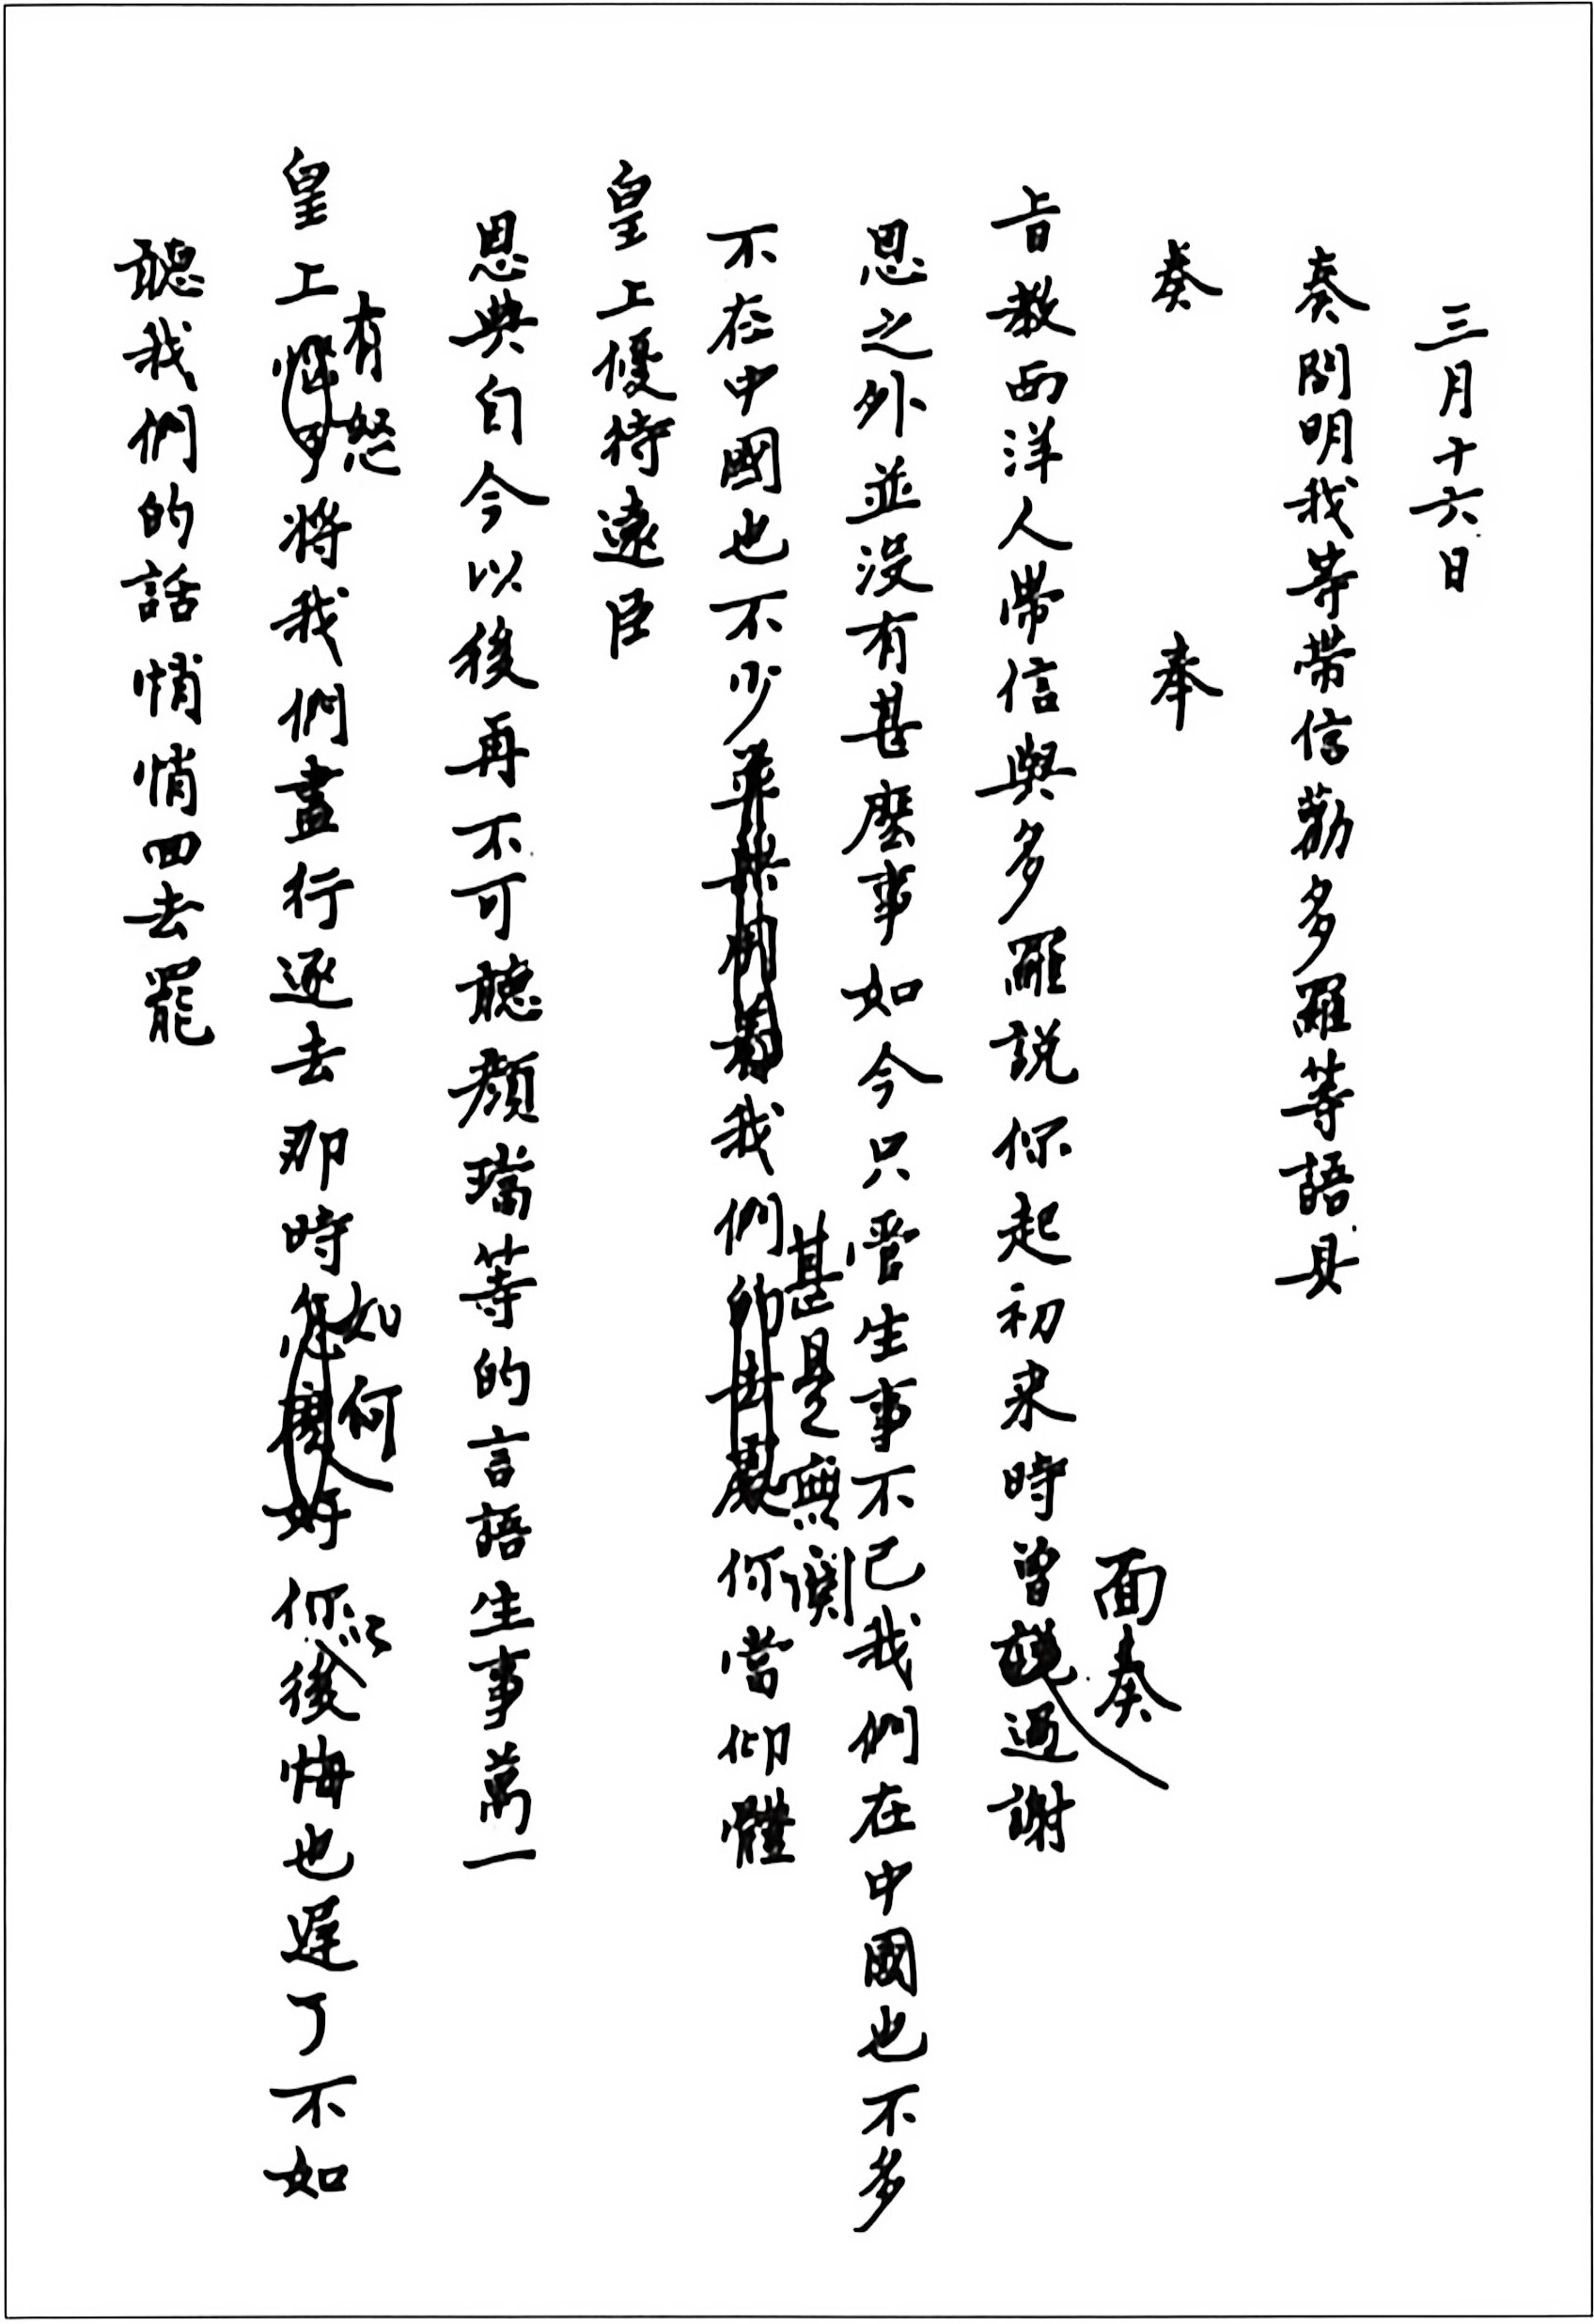
\includegraphics[width=\linewidth,height=.76\textheight,keepaspectratio]{assets/figures/kangxi-grimaldi-letter.png}
\caption*{图5.1\quad 康熙批改闵明我劝多罗信}
\BookFloatNotes{图片来源：陈垣编，《康熙与罗马使节关系文书》，文件3。}
\end{figure}%
不能辨别其真伪，康熙让礼部通过他们的渠道通知各地方。很快，%
地方上的传教士也发现他们领的印票在当地是有用的。在地方官眼%
里，这个票是内务府发的，相当于确认了这些传教士是康熙府中之%
人。无论从康熙规定领票的初衷还是后来的实际操作上看，康熙要%
求领票其实跟今天开车需要领驾照相类似，目的是为了规范，而不%
是为了限制。%
% 原书页码：200；标题
\subsection{小结}
\par
% 原书页码：200–201；段落（跨页续段）
民国时期，美国哈佛大学学者费正清在研究清代的外交中，提%
出了清朝的朝贡体系。其中最重要的一篇是20世纪40年代发表的%
总结清朝来华使团的论文，题目是《关于清朝的朝贡体系》。\NoteRef{5}{91}费正%
清总结了清代官方历史文献中的所有来华使团，他当时已经注意到，%
尽管清代的官方历史对各种大大小小的人华使团都有详细记录，但%
教皇派到康熙朝的使团竟然在大清所有的官修史书中都未见记载。%
俄罗斯派往康熙朝入京的使团有三个，但其中两个也都未见任何记%
录。而这几个未见记录的使团在西方文献中都很有名，费正清把它%
们单独列人一张表格中，但他没有能给出解释，为什么官修清史会%
出现选择性的记录和缺失。如果是因为别的原因，比如雍正不喜欢%
传教士，所以把教皇派到康熙朝的两个使团的记录删去了，那为什%
么所有的大清官修史书中，又都记录了教皇派到雍正朝的第三个使%
团？俄罗斯三次派到康熙朝的使团（1676、1693、1720）也是这样，%
其中第一次1676年的使团在清官修史书中有记录，而后面两次就没%
有任何记录。如果是有什么我们后人不知道的原因，又为什么只删%
除后面两次，而保留第一次？%
\par
% 原书页码：201；段落
我们知道了康熙接待多罗的各种细节以后，原因就一目了然了。%
没有记载并非后人的删除，而是因为康熙从一开始就把接待教皇使团%
当作他的家务事在操办，从头到尾都没有让朝廷部门经手。在康熙的%
安排下，整个过程都是他的内务府在一手操办，所以整个接待就不是%
外交活动了，而是他的家务事。因为是家务事，朝廷的史官自然就没%
有参与，也就没有留下记录。同样的原因，雍正在1725年接待教皇%
来使的时候，全程都交给了礼部在办理，属于朝廷接待，整个过程朝%
廷的史官都记录了。俄罗斯使团也是这个模式，第一次使团是礼部接%
待的，所以有记录，而后面两次都是康熙的内务府承办的。%
\par
% 原书页码：201；段落
康熙与耶稣会神父之间的关系决定了康熙接待教皇来使的各种安%
排。康熙在朝廷上是皇帝，而在他的家中，按照满人的传统，他是主%
子。他自然要照顾长期在他家庭圈子中的传教士。按康熙对传教士说%
的话，他同意接待多罗，是看在“豢养尔等多年”的分儿上。“豢养”%
二字在中文中是养家畜时使用的词语，特别是“豢”字，最早是用来%
表示喂猪（豕）的。满人主奴关系下，最早奴才和动物是一样的，主%
子负责奴才的吃喝，像养动物一样养奴才。在这个特殊的语境下，“豢%
养奴才”这样的表达才大量使用。%
\par
% 原书页码：201–202；段落（跨页续段）
最后康熙决定用内务府把多罗使团当成私人关系接待，接待中%
吃吃喝喝，都是很典型的满人主子宴请待客之道。多罗后来慢慢明%
白了康熙和耶稣会神父之间的关系后，很无奈，因为无论他和康熙%
说什么，耶稣会神父都要按照他们的想法给康熙分析一遍。多罗在%
一封信中说道：“耶稣会神父在宝座的背后，为了他们的自私想法，%
误导着皇帝。”\NoteRef{5}{92}%
\par
% 原书页码：202；段落
康熙对耶稣会神父的信任，从中国历史上来看都是很不寻常的。%
比如他决定派遣使节到欧洲，选派的人员都是听他周围耶稣会神父推%
荐的。其中的薄贤士没有在康熙身边当过差，康熙只是看过他写的对%
中国礼仪问题的论说，就决定选派他代表自已出使。薄贤士自己都有%
些意外，在谢恩中特别感谢康熙的信任。\NoteRef{5}{93}3康熙对待耶稣会神父的一%
切都是基于他和这些神父长久以来的私人关系。这和礼仪问题及天主%
教教义都没有多大关系。他容纳天主教也好，接见多罗也好，都是看%
在他周围神父的面子上的。所以只要他和这些神父的关系不变，他对%
天主教的态度也不会有大的变化。对于多罗来讲，他的出使在最后阶%
段失败了，他人华的所有目的都没有达到。但是对于耶稣会神父和康%
熙来说，与罗马的交流才刚刚开始。康熙派出的两个去罗马的使节带%
着希望出发了。%

\clearpage\markboth{第六章\quad 彼得大帝使团和教皇新使团}{第六章\quad 彼得大帝使团和教皇新使团}
% 第六章 彼得大帝使团和教皇新使团
% 原书页码：203；标题
\section{彼得大帝使团和教皇新使团}
\par
% 原书页码：203；段落
1707年2月7日，多罗在南京发布了教皇特使谕令，公开反对康%
熙的领票要求，阻止在华传教士去领票。\NoteRef{6}{1}在华洋人没料到多罗会这样%
公然反对康熙，纷纷写信给北京的神父，希望他们从中调停，以免龙%
颜震怒。\NoteRef{6}{2}%
\par
% 原书页码：203–204；段落（跨页续段）
说来也巧，这年春天，资格最老、在康熙身边已有三十四年的葡%
萄牙神父徐日升（1673年人京）得了头痛病，病得很厉害，他在信中%
说，他的头痛病好不了就是和多罗有关。\NoteRef{6}{3}在康熙身边二十几年的安多%
神父（1685年人京）这个时期也病了，说自己病重到信都写不了了。\NoteRef{6}{4}%
如果说这两位神父可能是装病的话，那么假不了的是53岁的张诚神%
父突然在3月份去世了。张诚1688年人京后就一直跟在康熙身边。%
无论是奔袭塞外还是南巡，康熙都把张诚带在左右。由于张诚和多罗%
都是法国人，多罗在京的时候，他是接待多罗的主要负责人。多罗走%
后，他也就成了多罗问题的责任人。张诚在去世之前并没有什么基础%
疾病，直到头一年12月，他都还忙着处理多罗人华后的很多遗留问题。%
但他的死很可能与多罗有关。因为张诚死后有一点很不寻常，就是康%
熙没有任何表示，没有给他举行葬礼，一句慰问的话、一两银子都没%
给。翻看历史就很清楚，康熙对传教士很照顾，根据亲疏远近，康熙%
多少都会对死去的传教士有抚恤。张诚做过康熙的老师，后来又常年%
跟在康熙身边。一直到他去世前几个月，他都还在康熙身边。他突然%
去世，而康熙没有任何表示的最大可能，就是康熙这段时间正在问责%
张诚，他很可能是处于极大的压力之下再加上得病才去世的。\NoteRef{6}{5}%
\par
% 原书页码：204；段落
最早在是否要接待多罗这个问题上，北京耶稣会神父内部是有分%
歧的。作为法国耶稣会神父的负责人，张诚主张接待，反对的葡萄牙%
神父们后来让步了。\NoteRef{6}{6}多罗人京后，和葡萄牙神父的负责人徐日升之间%
有很大矛盾。按照德国耶稣会神父的记载，多罗在众多神父在场的情%
况下，公开羞辱了徐日升神父。说他到中国后根本不是个神父，就是%
个艺人（artisan），还反问徐日升：你到中国是“用手传教”的吗？徐%
日升神父和康熙私交很深，他也确实让康熙喜欢上了西洋音乐。后来%
康熙的内务府中还有西洋交响乐队，彼得大帝的俄罗斯使团1720年到%
访北京时还听过这支乐队的演奏。康熙组织编撰的音乐著作《律吕正%
义》有一卷专门讲西方音乐知识，就是徐日升神父写的。站在徐日升%
神父的角度，他是希望用他掌握的音乐知识来接近康熙，从而换取康%
熙对天主教的优容。被多罗当着众多神父的面说成艺人，他是很委屈%
难过的。因为在天主教语境中，“艺人”类似于中文里的“戏子”。虽%
然当时欧洲整体并没有歧视艺人，但是在宗教环境中，把一个神父说%
成艺人有很大的羞辱意味。北京传教士大多同情徐日升神父，因为他%
们理解徐日升神父的不得已和委屈。\NoteRef{6}{7}%
\par
% 原书页码：204–206；段落（跨页续段）
多罗是教皇特使，在教会内部级别又高过北京耶稣会的神父，所%
以他面对耶稣会神父时态度居高临下，说话也不客气。他在责骂徐日%
升神父的时候，法国、葡萄牙等多国神父都在场，平时说法文的多罗，%
直接用所有神父都能听懂的拉丁文对着徐日升神父开骂：“你，你，你，%
给我站起来，你有罪，没有资格坐下………”\NoteRef{6}{8}这样的场景在耶稣会神父%
的《北京纪事》中被记录下来，用来反映多罗对北京传教士的傲慢。%
在北京，多罗唯一要给一些面子的耶稣会神父就是张诚。张诚在许多%
问题上也劝过多罗。多罗离开北京后，张诚也尽其所能地收拾多罗留%
在北京的烂摊子。颜珰觐见康熙后闯了祸，张诚拨出专款，给颜珰做%
路费，帮助他赶紧离开中国回欧洲。后来，一直很反感多罗使团、当%
时负责内务府的康熙大皇子，又发现多罗的翻译毕天祥神父在四川还%
有官司没解决，张诚又出面各方打理疏通。张诚在1706年12月给当%
时在南京的多罗写了封长信，告诉他离京后留下的各种麻烦事。也是%
在这封信中，张诚告诉多罗康熙将要实行领票。现在看这封长信，张%
诚最主要的目的，是要跟多罗说他留下的麻烦已经够多了，现在康熙%
皇帝又开始要求领票了。\NoteRef{6}{9}潜台词是劝多罗赶紧离开中国。但张诚完全%
没有料到，多罗后来会公开反对传教士去康熙那里领票。这样一来，%
他就变成了给多罗通风报信的人。张诚受过康熙很多恩惠。康熙北出%
大漠，追击噶尔丹都带着张诚。张诚留下了详细的日记。从中可以看%
出，康熙随时都把他带在身边，他记录下了康熙接见塞外蒙古各部落%
的瞬间。很多接见现场，连跟出去的朝廷史官都没有机会参与。还有%
很多他和康熙的谈话，可以说都是朋友之间的对话。所以当多罗谕令%
发出来，他被划到多罗一边后，于公于私，张诚都很委屈，百口莫辩。%
当然，也没有直接证据证明张诚的死和多罗相关。但是康熙在张诚死%
后，对他这个鞍前马后十几年的老熟人，没有任何表示，就足以说明%
问题。张诚死前面临的压力可想而知。%
\par
% 原书页码：206；段落
面对多罗的谕令，几个月来一直称病不出的一位老神父出面了。%
他就是68岁的闵明我。闵明我也是耶稣会神父，他1671年人京后%
做南怀仁的助手，在钦天监里当差。由于闵明我有朝廷官衔，这在%
天主教内部是一个很有争议的问题，所以多罗人京以后，闵明我一%
直避免和多罗有任何接触。1707年3月底张诚死后，徐日升和安多%
也都病重，闵明我作为北京神父中的元老，4月不得不出来收拾残局。%
简单来说，闵明我神父处理多罗问题的策略就是把多罗和教皇区分%
开来，向康熙解释多罗有问题是他个人的问题，他的观点不能代表%
教皇。4月27日，康熙身边的奴才赫世亨和赵昌禀报康熙，他们给%
闵明我带去口谕，命他写信给多罗。闵明我告诉赫世亨和赵昌，他%
们传教士已经多次寄信给多罗，他都不听；而且多罗还警告说要向教%
皇告他们的状。闵明我还讲，他们每次写信都是好言相劝，但这样%
多罗反而以为他们怕他。闵明我的原话是：“以和语寄信，尔似乎以%
为我等惧怕于尔。”闵明我汇报给康熙，说不要再理会多罗了，应该%
直接联系教皇，康熙表示同意，这样康熙也就在多罗这个问题上翻%
篇了，不再继续和多罗纠缠，只是让广东官员运作，联系澳门的葡%
萄牙人把多罗软禁在了澳门。%
\par
% 原书页码：206–207；段落（跨页续段）
康熙和北京耶稣会神父大概都没有想到，他们派去欧洲的人，一%
去十多年都没有消息回来。一直要到1720年，才等来教皇的第二支赴%
华使团。从康熙1706年派葡萄牙耶稣会神父龙安国和法国耶稣会神%
父薄贤士去欧洲算起，康熙等了十四年。这期间康熙早年身边信任的%
传教士都先后去世了。除了前面提到的1707年去世的张诚神父，徐%
日升在1708年，安多在1709年，闵明我在1712年先后离世。被软%
禁在澳门的多罗也于1710年过世。%
\par
% 原书页码：207；段落
康熙不厌其烦地和欧洲沟通，表面上好像一波三折，但内里恰恰%
反映出康熙对欧洲的耐心和对北京神父们的关心。本书反复提到的红%
票，就是康熙在这等待中发往欧洲的寻人启事。康熙和所有人并没有%
不同，当一个人不厌其烦地干一件事的时候，往往是有原因的。我们%
需要了解的是其不厌其烦的动力。而且当我们细察康熙和教皇第二使%
团的交往以后，我们就会发现康熙对教皇第二使团很满意，根本就没%
有过禁止天主教的想法。雍正后来要禁教，并不是康熙的意思。\NoteRef{6}{10}%
% 原书页码：207；标题
\subsection{十四年的等待}
\par
% 原书页码：207；段落
教皇的两个人京使团，当事人和后来的史家都有提及，从不同角%
度都有记录。但是康熙等待第二个使团来华的十四年却无人关注过。%
康熙在这十四年中，对他派出的使节有过无数次的关心和挂念。这些%
关心和挂念，单独看只是一句问询，一个小举动，但把他一次次询问%
汇集到一起，就是十数年的坚持。本书中出现的红票，就是康熙挂念%
他使节众多举动中的一个。教皇派出的第二个使团是对康熙十多年等%
待和挂念的一个正式回复。%
\par
% 原书页码：207–208；段落（跨页续段）
多罗离开北京不久，1706年10月17日，康熙派出葡萄牙耶稣会%
神父龙安国和法国耶稣会神父薄贤士代表他出使罗马。1707年1月，%
薄贤士在广州登船后，给北京的闵明我神父写了一封信，说他们二人%
已经登上了一艘坚固的大船，船上的水手对他们很好。他让闵明我神%
父转达康熙，让康熙放心。这是二人留给康熙的最后信息。二人选择%
了穿越太平洋，从美洲返回欧洲的航线。他们抵达巴西后，在8月7%
日给罗马耶稣会总会长写了封信，告知二人即将返欧，并且通知会长%
二人将先分别回到自己的国家，然后再到罗马会合。\NoteRef{6}{11}二人在巴西，%
为了分散旅途中沉船的风险，分别登上了两艘不同的船去欧洲。但不%
幸的是，在1708年1月，两艘船都在途中遇到海难沉没了。\NoteRef{6}{12}%
\par
% 原书页码：208；段落
在两位神父离开北京后的第二年秋天，也就是1707年的秋天，康%
熙就开始打听二人的消息了。根据现存的满文奏折，康熙派他身边的%
奴才去问了闵明我，闵明我回答他什么信息都没有收到。\NoteRef{6}{13}因为1707%
年春天多罗宣布了谕令，又发生了许多事，加上还没有收到前次使节%
的消息，康熙决定再派两位使节去罗马，更完整地传达他的意思。这%
次康熙派出的是耶稣会艾若瑟和陆若瑟二位神父出使。二人于1707%
年10月27日离开北京去往澳门，他们在1708年1月14日登上了一%
艘葡萄牙的船，从印度洋线路前往欧洲。这次行程中艾若瑟还带上了%
他的中国弟子樊守义。樊守义在欧洲待了数十年，后来回到中国，一%
直到乾隆中期去世。身后留下了《身见录》，记载了他的欧洲行程。%
\par
% 原书页码：208；段落
艾若瑟一行于1708年9月抵达葡萄牙里斯本，葡萄牙国王接见了%
他们。1709年2月艾若瑟抵达罗马，并见到了教皇。教皇没有同意艾%
若瑟关于中国礼仪的意见，坚持他之前禁止中国天主教徒参与中国传%
统礼仪活动的决定。同时，教皇让艾若瑟留在欧洲，不要返回中国。\NoteRef{6}{14}%
\par
% 原书页码：208–209；段落（跨页续段）
艾若瑟一行在欧洲的行踪，康熙并不知道。不过康熙没有忘记他%
派出去的两个使团。在1708年8月的时候，康熙派人去问北京的神%
父们，怎么这么久他们都没有到康熙处报告和请安。正常情况下，7、%
8月份是西洋帆船乘着季风到来的时节，所以康熙这时候专门派人去%
问询。闵明我汇报说，他确实早就准备给皇帝请安了，但他在等消息，%
希望有了使团确实的消息以后，一并向康熙奏闻。闵明我还补充说，%
现在正是西洋船来华的时节，就算他不能收到两个使团的来信，也会%
多多少少从其他渠道得到一些关于两个使团的信息。\NoteRef{6}{15}闵明我的回答%
说明康熙一直在期盼消息，而且这种期盼给了闵明我很大压力，以至%
于他都在回避向康熙请安了。一个月以后，1708年9月23日，闵明%
我不得不上报康熙，被他派出去测量长城、绘制地图的法国传教士白%
晋从马背上摔了下来。在汇报完这件事后，闵明我在末尾提到他还是%
没有收到两个使团的消息。\NoteRef{6}{16}%
\par
% 原书页码：209；段落
等了两年什么也没等到，康熙在1709年春决定增加信息收集的渠%
道。在4月份，也就是西洋船到来之前，他通过朝廷的官方渠道，下%
旨给江西、福建的巡抚，以及两广总督，让他们留意西洋过来的包裹%
和信件，有新的发现立刻上奏。下给这几位封疆大吏的谕旨都是中文%
写的，内容基本也是一样，分别发给了他们。\NoteRef{6}{17}这几位封疆大吏收到%
谕旨的时候，应该都比较惊讶，不知道为什么康熙会突然让他们关注%
西洋来信来物，而且谕旨又没有明示到底要关注西洋来的什么，几人%
也不知道该怎么回奏。几位封疆大吏不知是否私下联系过，但他们的%
反应都是一样，猜康熙所谓的西洋物品是红酒，于是都到自己管辖地%
区去找西洋人要洋酒，然后又把洋酒派人送到北京进献给康熙。\NoteRef{6}{18}到%
这年8月的时候，康熙还是什么消息都没有。他又派人去问北京传教%
士，但他们也没有收到任何信息。\NoteRef{6}{19}%
\par
% 原书页码：210；段落
1710年3月，康熙通知两广总督，让他关注所有将要来华的西洋%
船只，一有消息，迅速奏闻。\NoteRef{6}{20}8月，两广总督禀报多罗去世。\NoteRef{6}{21}康熙%
在回两广总督的折子上，让他继续关注西洋来船，有信件和消息都迅%
速奏报。\NoteRef{6}{22}1711年夏天，康熙还是没有收到任何消息。于是又几次派%
人去问北京传教士，仍然未果。\NoteRef{6}{23}%
\par
% 原书页码：210；段落
1712年8月，康熙终于等到了消息。此时距离第一批使节离开北%
京已经六年。葡萄牙人苏霖神父（José de Suarez，1656—1736）上奏康%
熙，他从欧洲朋友的来信中得知艾若瑟见到了教皇，人现在还在罗马。%
同时苏霖神父还解释说，这是他刚刚得到的最新消息，这封信所在的%
葡萄牙大船在人华途中耽搁了。苏霖专门解释这个细节，是因为不久%
前康熙才派人问过北京传教士。尽管苏霖解释了，康熙还是不相信，%
认为这些神父有意隐瞒。\NoteRef{6}{24}好在两天后，康熙收到一封沿海官员的奏报，%
奏报中也提到了苏霖神父说到的大船，也说这条船延误了。\NoteRef{6}{25}这样康%
熙才相信了传教士的话。10月1日，苏霖神父再次上报，他又收到一%
封信，也提到艾若瑟已经到了罗马。信中还说，葡萄牙国王接见过艾%
若瑟，而且还派遣了使臣去罗马，劝说教皇不要听信多罗的话。\NoteRef{6}{26}%
\par
% 原书页码：210–211；段落（跨页续段）
康熙收到这些消息后，也算一块石头落地，好歹终于有使节到%
了罗马。这之后，康熙开始等待使节回归了。两年前，也就是1710年，%
广州巡抚范时崇奏报过，他从澳门人那里听说，康熙派出的龙安国%
和薄贤士已经沉船身亡。范还请旨康熙应该如何处理当时软禁在广%
州的几位神父。那几位神父是康熙交给范时崇，让他等龙安国和薄%
贤士回到中国以后再发落的。康熙告诉他，什么都不要变，继续照%
看那几位神父，等待他派出去的第二个使团回归。\NoteRef{6}{27}不过，康熙对%
两位神父去世的信息持怀疑态度，他们的死讯当时也无法证实真假。%
康熙交代沿海官员继续查证。后来1718年另一位巡抚上的折子中提%
到他从西洋人那里得到信息，龙安国和薄贤士二位神父确实已死亡，%
验证了范时崇的报告。\NoteRef{6}{28}%
\par
% 原书页码：211；段落
1712年以后，现存的奏折中开始有不少沿海官员上报西洋人和物%
的折子。以前都不知道为什么沿海官员这时期突然开始定期报告西洋%
来船和物了，这都是因为康熙挂念他派出去的使节的缘故。\NoteRef{6}{29}特别要%
注意的是1708至1712这几年，是康熙人生中比较艰难的几年。这一%
时期正是康熙被太子废立问题搞得焦头烂额的时候。1708年康熙废太%
子，1709年又复立太子，1712年再废太子。用今天的话来说，就是%
康熙在百忙之中，被家庭内部问题搞得心烦意乱之际，还惦记着他派%
去欧洲的神父们。这些汇报西洋人事的奏折为后人提供了很多有用信%
息。比如著名的宫廷画师，后来一直活跃到乾隆中期的耶稣会士郎世%
宁，他的入华消息最早就是广东巡抚1715年汇报给康熙的。\NoteRef{6}{30}%
% 原书页码：211；标题
\subsection{康熙发给欧洲的公开信}
\par
% 原书页码：211–212；段落（跨页续段）
1715年3月19日，教皇重申了1704年他签署的关于禁止天主%
教徒参与中国礼仪活动的谕令。教皇知道他的谕令发出去了十年，相%
关的争论还在持续。他进一步确认之前的决定，希望这样能够平息争%
端。\NoteRef{6}{31}一位英国船长在1716年8月来华贸易的时候，把教皇关于中国%
礼仪的决定全文带到了中国。\NoteRef{6}{32}康熙从北京耶稣会神父那里看到了该%
决定的翻译。康熙很气愤，认为他派出去的人都没回来，而且他已经%
等了近十年，不能就这样接受一份随便抄来的教皇决定。于是康熙决%
定主动出击，既然等不回他的使节，他就昭告天下。本书所写的红票%
就是在这样的背景下产生的。%
\par
% 原书页码：212；段落
康熙让内务府印刷的红票，是一封让往来的西洋船只带回欧洲的%
公开信。这封公开信上有汉文、满文、拉丁文三种文字。由于印刷的%
墨色为朱砂红色，历史上又称“红票”。红票交给广东官员，让他们%
分发给所有“有头面”的西洋人，让他们带回欧洲。同时，康熙也把%
红票交给俄罗斯的往来官商，让他们也帮忙传递给欧洲。%
\par
% 原书页码：212；段落
红票的全文如下：%
\par
% 原书页码：212；段落
{\bookkai 武英殿等处监修书官伊都立、王道化、赵昌等字，寄与自西洋来}%
{\bookkai 的众人。我等谨遵旨于康熙四十五年已曾差西洋人龙安国、薄贤士，}%
{\bookkai 四十七年差西洋人艾若瑟、陆若瑟，奉旨往西洋去了。至今数年，不}%
{\bookkai 但没有信来，所以难辨真假。又有乱来之信，因此与鄂罗斯的人又带}%
{\bookkai 信去，想是到去了。必竟我等差去人回时，事情都明白之后，方可信}%
{\bookkai 得。若是我等差去之人不回，无真凭据，虽有甚么书信，总信不得。}%
{\bookkai 因此，唯恐书信不通，写此字，兼上西洋字刊刻，用广东巡抚院印，}%
{\bookkai 书不封缄，凡来的众西洋人，多发与带去。康熙五十五年九月十七日。}%
\par
% 原书页码：212；段落
康熙红票的内容没有讲道理，也没有表明他任何观点，只是简单陈述%
一个事实，就是我派了人出去，但都没回来。康熙发出这封信的时候，%
其实已经知道派出去的四个人中有三个已经去世了。四个人的名字一%
起点出来，就是要教皇给个说法。%
\par
% 原书页码：213；段落
康熙红票中玩的这个计策，他早年就用过。在与噶尔丹汗交战时%
期，康熙从一个俘虏那里得知达赖喇嘛早已圆寂多年，统治西藏的桑%
杰嘉措却一直对大清隐瞒这个消息。康熙当时不愿意跟西藏方面把关%
系闹僵，这样很难收场。康熙在他的使节离开北京前，秘密跟使节交%
代，去了西藏不要质问达赖去世的消息，只需要坚持和达赖会面，看%
桑杰嘉措怎么说。\NoteRef{6}{33}康熙红票就是这样，把四个人的名字都写出来，%
要教皇给一个交代。红票的内容是康熙用满语口述的，汉语是他身边%
的奴才翻译的。文字没有经过康熙的内阁大学士润色，完全是口语，%
而且细读还不通顺。这也说明康熙一直坚持他跟罗马的联系是他的私%
事，不把朝廷里面的人牵涉进来。%
\par
% 原书页码：213；段落
红票传到欧洲以后，确实给教皇带来了很大的压力。艾若瑟回%
到欧洲，各国的教会内部早有耳闻。红票让欧洲知道原来艾若瑟是%
康熙皇帝的使节。这让教皇在道德层面很难堪。当时18世纪的欧洲%
已经很开明，拦着别国的使节不让回去是不可接受的。教皇在1717%
年收到红票后，赶紧召见了艾若瑟，让他回去复命，并让他用身体%
原因为借口解释为什么这么多年没有回去。\NoteRef{6}{34}艾若瑟走后，教皇迅速%
筹备了第二个赴华使团。教皇准备了一封长信让使团带给康熙。这%
封长信除了官方问候文字，还用了很多笔墨向康熙解释四位使节的%
遭遇。\NoteRef{6}{35}%
\par
% 原书页码：213–214；段落（跨页续段）
对于康熙来说，红票达到了预期的效果。艾若瑟被允许回大清，%
同时教皇又派了第二个使团亲自来解释。不幸的是，艾若瑟病逝在回%
大清的船上。他的汉人弟子樊守义守着他的棺材一起抵达广州。广东%
巡抚向康熙报告了樊守义的回归。康熙看完报告很疑惑，命令巡抚详%
查樊守义，因为康熙怀疑艾若瑟是在路上被害死的。但是，巡抚严查%
以后，并没有发现艾若瑟之死有可疑之处。康熙还是不相信，后来见%
到教皇的使节，还当面发火说道：“中国所使之人，一字不回，都暗害%
杀死。”\NoteRef{6}{36}%
% 原书页码：214；标题
\subsection{康熙的耐心}
\par
% 原书页码：214；段落
康熙皇帝文韬武略，南征北战，是世界历史上都赫赫有名的君主。%
无论从哪个角度看，康熙都完全可以按照他的想法决定传教士、天主%
教以及礼仪等众多问题。他完全有权力这样做，根本不需要和欧洲任%
何一方啰唆。但在与罗马的沟通上，康熙显示出了非同寻常的耐心。%
就连到京的俄罗斯使团也看出了这个问题，很惊讶为什么康熙大帝会%
有耐心跟天主教争辩这些理论问题。俄罗斯彼得大帝派使团1720年%
11月9日入京，比教皇使团早二十五天。两个使团到北京后都互相%
知道，康熙还一起接见过双方使团。双方也都用北京的传教士在做翻%
译，两边使团成员私下也有往来。俄罗斯的随团医生约翰·贝尔（John%
\space%
Bell）是苏格兰人，在他的旅行游记中就记录了康熙参与中国礼仪问题%
的争论，而且还评价道：%
\par
% 原书页码：214；段落
{\bookkai 从任何角度来审视，一个异教的皇帝有兴趣参与到天主教内部的}%
{\bookkai 纷争中去都是一件很奇怪的事。\NoteRef{6}{37}}%
\par
% 原书页码：214–215；段落（跨页续段）
约翰·贝尔解释说中国礼仪问题的争论是天主教内部的耶稣会和多明%
我会两边的争论。他作为基督教新教徒都没有兴趣了解，因而很惊讶%
康熙会有兴趣掺和进去。西方研究康熙的权威、耶鲁大学的史景迁教%
授，在1990年代一次关于“中国礼仪之争”问题的研讨会上，也对%
康熙参与到争论里面表示很疑惑。史景迁这样评价道：%
\par
% 原书页码：215；段落
{\bookkai 简单来讲，康熙完全可以把所有中国礼仪相关的争论都当成无稽}%
{\bookkai 之谈，那么这样我们也就不会在这里（开这个会）了。或者，他就坚}%
{\bookkai 持他自己的想法，无论想法是什么，他都可以坚持。他有权力这样做。}%
{\bookkai 他完全可以把一些传教士赶出中国。但他没有这样做，而是选择参与、}%
{\bookkai 争论、劝解，有时候还要发火。他真的很投入地在参与。\NoteRef{6}{38}}%
\par
% 原书页码：215；段落
史景迁认为康熙的参与不同寻常，他完全可以简单粗暴地处理这个问%
题，但他没有。那为什么康熙会耐着性子参与到这场耗时耗力的争论%
中去呢？%
\par
% 原书页码：215–216；段落（跨页续段）
流行的说法是康熙是要捍卫中国文化，要从道理上说服西方。前%
人有这样的看法也不奇怪，因为一直以来，北京耶稣会神父就有意要%
把康熙塑造成文化捍卫者的形象。他们希望这样罗马教廷可以看在康%
熙皇帝的权威上有所让步。在欧洲的文化传统中，耶稣会神父把康熙%
描绘成文化捍卫者，完全吻合欧洲对东方开明皇帝的想象。他们自己%
心中的伟大皇帝就应该这样。\NoteRef{6}{39}因此，耶稣会神父对康熙这样的人设%
塑造在欧洲很成功。康熙身边的乐师、遣使会派到中国的德里格神父%
（1671—1746）就反复说过，康熙不像耶稣会神父说的那样，他是可以%
接受不同意见的君主，而且完全有可能接受教皇对中国礼仪的禁约。\NoteRef{6}{40}%
在德里格之前，多罗根据自已和康熙的接触也说过相同的话，认为康%
熙是有可能接受禁约的。多罗认为，之所以康熙不能接受，是耶稣会%
神父从中作梗，误导康熙。多罗写过信直接点明这一点。\NoteRef{6}{41}但是，历%
史是后人根据自己的理解书写的。无论是多罗还是德里格，他们留下%
的资料、信件，在后人看来，都有很多偏见，不够客观。最主要的是，%
他们的文字完全没法和耶稣会神父留下的记录做比较。耶稣会神父对%
事件做的记录，都是丝丝人扣，各种材料互相印证，让人无从反驳。\NoteRef{6}{42}%
这也是为什么后世基本都相信耶稣会神父们的记录的原因。%
\par
% 原书页码：216–217；段落（跨页续段）
但一些新出现的汉文、满文奏折，说明康熙确实如德里格、多罗%
所言，是有可能在中国礼仪问题上接受不同意见的。1715年，德里格%
给康熙上过一封汉文密折，折子开头就希望康熙保密，不要把折子内%
容透露给他身边的奴才，因为那些奴才都是站在耶稣会神父一边的。\NoteRef{6}{43}%
德里格的折子的核心是向康熙说明为什么那么多年都没有他两个使团%
的消息。按德里格的说法，是耶稣会神父有意屏蔽了欧洲过来的消息。%
德里格在这封折子中向康熙讲了教皇禁约的大概内容，同时告诉康熙%
欧洲所有天主教修会都表示遵守教皇禁约，而且特别点出在罗马的耶%
稣会总会长都已经明确表示了要遵守教皇禁约。德里格告诉康熙，中%
国地方上的耶稣会神父早就收到了罗马发来的教皇禁约，但是以纪理%
安为首的北京耶稣会神父阻止教皇禁约在中国流传。这就是为什么所%
有在华西洋人都知道了新传来的禁约，而没人禀报给康熙的原因。为%
了说明耶稣会神父的霸道，德里格还提到了西洋人罗若德。\NoteRef{6}{44}1712年%
罗若德在澳门上交给广东巡抚一封教皇寄给多罗的信件，那时多罗已%
经去世，他就转给大清朝廷。德里格说，在澳门的耶稣会神父知道罗%
若德把信给广东巡抚后的当天晚上，就逼着罗若德登上了一艘离开澳%
门的船。%
\par
% 原书页码：217；段落
尽管德里格的奏折中很多事的真假无法查证，但他所说的罗若%
德一事是有据可查的。1712年10月11日，广东巡抚满丕上了一封%
满文折子，转交了罗若德的信。满丕在折子中还说，他收到罗若德%
的信后，专门去找广州的神父们鉴定过，广州的神父说信确实是教%
皇发出的。\NoteRef{6}{45}%
\par
% 原书页码：217；段落
除了封锁欧洲的消息以外，德里格还说耶稣会神父打着康熙的名%
义警告欧洲不要乱发消息人华。其中一封邮寄到欧洲的信，耶稣会神%
父是让康熙身边的奴才赵昌签字的，让欧洲不要把有关禁约的内容发%
到中国来。赵昌其实在欧洲的教廷那边已经小有名气，因为一直是他%
在替康熙打理所有跟西洋人有关的事务。当然，可以想象，康熙对德%
里格反映的事情应该是半信半疑的。一方面，德里格所言部分地解开%
了康熙长期的疑惑，为什么他的使节出发近十年，一点信息都没有发%
回来。另一方面，康熙也知道德里格和耶稣会神父是有矛盾的。康熙%
看完德里格的折子，并没有大的举动，只是吩咐把折子转给他的两个%
儿子看。%
\par
% 原书页码：217–218；段落（跨页续段）
最能反映康熙真实想法的是他私下的谈话。康熙虽然表面上坚持%
天主教和中国传统文化互通，不矛盾，因而天主教应该允许中国礼仪%
相关的活动。但私下康熙很清楚天主教教义和中国传统儒家有很多不%
相通之处。他表面上坚持的观点，并不是他内心的真实想法，不过是%
为了在天主教世界继续中国礼仪活动而硬着头皮坚持的。1711年6月，%
康熙还在翘首等待他的出访使节回复的时候，耶稣会神父白晋把他新%
写的《易经》注解拿给康熙过目。康熙看后很着急，下旨让他身边的%
奴才把所有在京的耶稣会神父叫到一起，告诉他们：%
\par
% 原书页码：218；段落
{\bookkai 览白晋所写一文，其中引语多为繁杂。日后若有颜珰、刘应一类}%
{\bookkai 人物出来，则必款款皆难解释。若不从今日起有所谨慎，朕亦无法解}%
{\bookkai 释或说明。所有西洋人应当共同商议为妥，决不可轻忽。\NoteRef{6}{46}}%
\par
% 原书页码：218；段落
颜珰就是反对天主教徒继续参与中国礼仪活动的核心人物，康熙和他%
的会面上一章已经讲到过。刘应（Claude de Visdelou，1656—1737）%
是法国耶稣会神父，他是法国国王选派，当年和白晋、张诚一起最早%
入华的五位法国传教士之一。康熙接见过他，也知道他。刘应在中国%
待过一段时间，学习了中文以后，强烈反对天主教徒参与传统中国礼%
仪活动。他是持反对意见中很有名的一位，也是对中国文化比较了解%
的一位。所以康熙这里特别提到了他。%
\par
% 原书页码：218–219；段落（跨页续段）
《易经》尽管是儒家六经之一，可以看作是哲学书，但说到底，这%
是一本传统占卜的经典。特别是里面的卦象卦图，这些和天主教教义%
是有根本冲突的。康熙很明白这一点，因此很着急，告诉北京传教士，%
要是你们写的这些《易经》的书落到了颜珰、刘应手中，这还怎么解%
释天主教和中国传统文化不矛盾？所以康熙对传教士说，如果你们这%
样写书，“朕亦无法解释或说明”。康熙说这句话，并不是他过于小心，%
而是他已经有过切身体会，要论述天主教和中国传统文化互通是不容%
易的。当年他和多罗会见的时候，多罗举出儒家主张为父报仇，而天%
主教不允许的例子，康熙就已经觉得不容易辩驳了。康熙明白，要是%
对方再把《易经》中的东西翻出来，那就更没有办法继续了。这也是%
康熙为什么要把北京全部传教士召集到一起，亲口警告他们的原因，%
而且还叮嘱他们“不可轻忽”。%
\par
% 原书页码：219；段落
尽管这段满文谕旨说的是让传教士小心，但这最直接地反映了康%
熙的真实想法。康熙知道也明白中西不调和之处有很多。从历史的角%
度看，康熙是一位很务实的君主，他一生并没有什么特别的坚持。作%
为一个国土同时横跨中亚、东亚的君主，他当然清楚各个文化有不同%
之处。佛教、藏传佛教、道教等哪一个宗教都和儒家传统学说有冲突%
矛盾的地方。康熙也不会天真地以为儒家和天主教教义是相通的。所%
以耶稣会神父笔下那个要捍卫文化传统的君主只是他们理想中的康%
熙，真实的康熙是一位现实的、没有文化偏执的皇帝。%
\par
% 原书页码：219；段落
那么到底又是什么原因使康熙能不厌其烦，耐着性子和欧洲保持%
联系呢？这正反映了康熙是个世故圆滑的皇帝。因为那时的康熙急需%
欧洲人和他们的技术。这种需求在当时是很现实的，无法以其他方式%
替代。耶稣会神父在康熙年轻时给他介绍了欧洲的文化技术，康熙知%
道的越多，对欧洲文化技术的兴趣就越浓，需求也越大。康熙在1700%
年以后，不止一次通知南方口岸的官员，注意发现欧洲过来的有真本%
事的洋人。后来，遇到有技术的西洋人，广东的官员自己就摸索出了%
一套方法，来鉴定这些人是否有真本事。擅长绘画的马国贤神父和擅%
长音律的德里格神父，都是广东官员先面试过一轮后，再奏报给康熙%
的。德里格神父还记录了他第一次见到康熙，康熙面试他音乐知识的%
场景：%
\par
% 原书页码：220；段落
{\bookkai 他（康熙）把翻译叫到宝座附近，再把我叫过去，就开始“考试”}%
{\bookkai 了。他先问我是否带来跟音乐相关的新东西。我回答说我有自己创作}%
{\bookkai 的新曲子。然后，他又问我创作中是否用了一些新方法，问我是否使}%
{\bookkai 用哆、来、咪、发、唆、拉音符来谱曲。我回答说我使用了。他问我}%
{\bookkai 是否会在“拉”之后添加“西”（这是法国教授音乐的方式），或者说}%
{\bookkai 有没有不用“西”这个音符的其他方法。他说的这个其他方法指的是}%
{\bookkai 意大利方法，在“来”这个音中有上升突变，在“拉”中有下降突变。}%
{\bookkai 我回答说使用哪个方法对我来说都是一样的，我用意大利的方式举例}%
{\bookkai 讲解了其中的变化。他问我是否会用哆、来、咪、发、唆、拉音符唱曲。}%
{\bookkai 我说我嗓子不好，唱起来不好听。尽管如此，他还是让我试一试。他}%
{\bookkai 开始唱起来，我跟着他唱，他很满意。然后他问我是否知道缩短的音}%
{\bookkai 符，像八分音符、十六分音符、三十二分音符。翻译遇到了一些困难，}%
{\bookkai 他们只好用手来比划。我其实已经明白了问题，但还是等他们解释。}%
{\bookkai 然后我回答说，我不仅知道这些音符，而且还知道它们的用处，知道}%
{\bookkai 没有它们很难写出好的曲子。他问我是否知道升音符（sharp）和降音}%
{\bookkai 符（flat），在这里我没有等翻译，因为还有很多事情要做，我看着皇}%
{\bookkai 帝，问他是不是这些……然后我开始用升调来唱出音符。他高兴地说：}%
{\bookkai “是，是，好，好，好。”\NoteRef{6}{47}}%
\par
% 原书页码：220–221；段落（跨页续段）
德里格和马国贤二人其实是由软禁在澳门的多罗推荐给康熙的，但康%
熙明显不在乎这些传教士的派系，只要有真才实学，他都求贤若渴。%
在后来的相处中，康熙并不喜欢德里格的个性，但康熙还是优容了他。%
德里格1711年入京后再没有回欧洲（马国贤1723年回去了），活到%
乾隆年间。他在中国谱的曲子流传至今，网上可以找到欣赏。%
\par
% 原书页码：221；段落
在有些领域，康熙和他儿子已经学得很深入了，他们在等欧洲的%
学术突破。比如1717年，得知在欧洲大学做过数学教授的戴进贤神%
父（Ignatius Kögler，1680—1746）到达了北京，康熙让他的三儿子去%
试探对方是否有真才实学，同时让三皇子特别问问欧洲有没有找出新%
的简洁的数学方法来获取平方根和立方根。懂数学的人都知道，平方%
根和立方根求解是有一定难度的。特别是立方根求解，涉及跟虚数相%
关的问题，欧洲在18世纪中期以后才完全解决。康熙有这样的数学%
兴趣，就注定了他需要和欧洲保持良好的关系。\NoteRef{6}{48}%
\par
% 原书页码：221–222；段落（跨页续段）
如果说学术兴趣是抽象的，那么康熙当时正在进行的国家项目则%
是实打实急需有技术的西洋人。1710年前后，在张诚、徐日升等老一%
辈传教士相继去世后，康熙在进行中的一些大项目急需西洋人，其中%
最著名的就是勘测疆域，绘制地图。\NoteRef{6}{49}康熙由于缺人手，不得不把白%
晋派到一线去勘测。当时白晋醉心于《易经》研究，不愿意去。他到%
西安以后不久，康熙收到奏报，说白晋从马上摔下，需要回京调养。%
康熙对此朱批第一句就是“白晋原先即不愿去”，他看出这是白晋逃%
避工作的借口，接着写道：“理当痊愈之日即以自力追上去。”意指他%
要真是坠马，就应该等病好了自己追上勘测的队伍。然而白晋竟然回%
京了。康熙不仅生白晋的气，连转奏的奴才赫世亨也一起骂了，因为%
他的说辞感觉是在帮白晋掩饰，康熙写道：“尔如此含混转奏，理应即%
行革职。”\NoteRef{6}{50}从康熙对白晋坠马一事发火来看，1710年前后，康熙确实%
缺人手。但做西方式的勘测，画地图，只能用西洋人。康熙越到晚年，%
与西方各方面接触越多，也越需要更多的西洋人。1718年，康熙吩咐%
两广总督：“西洋来人，内若有各样学问或行医者，必着速送至京中。”\NoteRef{6}{51}%
1721年，康熙去世前一年过寿时，当时在北京的葡萄牙耶稣会穆经远%
神父（1681—1726）建议葡萄牙国王选送西餐厨师给康熙作为寿礼。%
穆经远说他自己的厨师被康熙征调到御膳房去了。\NoteRef{6}{52}%
\par
% 原书页码：222；段落
康熙从接见多罗以后，无论是派遣使节还是期待使节回归，处处%
都显示他有很强的意愿与欧洲进一步联系。他发给欧洲的红票更是说%
明了这一点。教皇在收到康熙红票以前，已经在欧洲公布了他禁止中%
国礼仪的谕令，洋洋洒洒写了一大堆理由。而对比来看，康熙的红票%
全篇没有一句话在阐述他的想法和观点，他只写了一个内容，就是昭%
告欧洲：我派了两批使节到欧洲，人都没有回来。这样的公开信发到%
欧洲，很明显，目的就是要求回复，要求继续谈。理解到这一点，以%
及看到康熙在接待第二个教皇使团前的漫长等待，我们才能够真正理%
解康熙在和教皇使节谈判中的各种说辞。%
% 原书页码：222；标题
\subsection{彼得大帝来华使团}
\par
% 原书页码：222；段落
在教皇使团到来前，彼得大帝的来华使团在1720年11月18日抵%
达了北京。两个使团差不多时间先后抵京纯属巧合。彼得大帝使团到%
北京来是谈判贸易的。自从1689年签订了《尼布楚条约》后，俄罗%
斯与大清贸易往来频繁，尝到了与大清和平往来的好处。但1710年%
代以来，俄罗斯对华贸易日渐衰落。衰落的根源，按照今天的说法是%
市场经济竞争的结果。当时大清理藩院给俄罗斯的公函是这样解释的：%
\par
% 原书页码：223；段落
{\bookkai （大清）各种皮货甚为丰足。况广东、福建等沿海地方，每年又}%
{\bookkai 有西洋等国商船前来贸易，诸凡物品甚足，无人购买尔之商货。皮}%
{\bookkai 货乃寒冷季节需用之物，内地暑热，而且所来皮货又甚多。小康人}%
{\bookkai 家购买貂、鼠皮张缝制衣服，一件衣服将穿多年。富有之人虽然愿}%
{\bookkai 买，而尔属之人又高抬物价，因此不能卖出。遇有内库购买各种皮货}%
{\bookkai 时，尔商人不但不肯出售好皮货，反而高抬物价，暗中私自赊给无名}%
{\bookkai 商贩，此等商贩皆为贫穷之人，一旦无力偿还，则又再三求告监督催}%
{\bookkai 收。….\NoteRef{6}{53}.53}%
\par
% 原书页码：223；段落
当时俄罗斯卖来的皮毛制品价格太高，无法和欧洲国家从海路卖过来%
的皮毛制品相竞争。除了价格高以外，俄罗斯产品质量也没有南方海%
运过来的东西好。跟俄罗斯做生意的中国商贩，赊了俄罗斯的货款，%
最后还不上了，俄罗斯商人又在北京告官。为了两国和睦，如果中国%
商贩实在没钱还给俄罗斯商人，最后是康熙从内库拿钱出来赔付给%
俄罗斯商人。理藩院写了一大堆理由来告诉俄罗斯，贸易减少不可避%
免，\NoteRef{6}{54}归根到底是因为俄罗斯的商品在中国没有市场竞争力。当时俄罗%
斯正在欧洲一侧和瑞典等国打仗，争夺出海口，彼得大帝需要大清的%
贸易来支持他在欧洲的军事行动。1719年，彼得大帝派伊兹麦伊洛夫%
率团出使大清，目的就是来找大清谈贸易。出行前，俄罗斯知道大清%
对书写用词这些细节很在意，专门在称谓上做了特别安排。彼得大帝%
让使节带给康熙的国书，最后的落款是：“大皇帝的好友，彼得。”\NoteRef{6}{55}这%
样通过朋友相称，避免了称谓上出现高低之分。%
\par
% 原书页码：224；段落
从圣彼得堡到北京，整个使团两百多人，停停走走，走了十六个%
月才到达北京。随团医生约翰·贝尔在游记中说，他估计速度快的%
话，应该半年时间可以从圣彼得堡到北京打个来回。\NoteRef{6}{56}使团到了北京，%
受到了康熙的热情接待。康熙一向重视与俄罗斯的关系，从国家战略%
层面讲，他一直认为大清最大的敌人是西北还没有归顺的蒙古部落。%
1720年，西北依然不太平。康熙派出他最得力的皇十四子前往处理甘%
肃、新疆、西藏这些地区的边务。所以，康熙对俄罗斯使团来访的举%
动也很欢迎。对康熙来说，能通过贸易稳住俄罗斯，把俄罗斯变成自%
已的盟友，是代价最小的解决大清北方地缘政治问题的方式。%
\par
% 原书页码：224；段落
俄罗斯使团是带了彼得大帝信函来华的正规使团，同时也提前通%
知了礼部和理藩院。本来是要这两个朝廷部门负责接待使团，但使团%
到了北京后，和礼部以及理藩院主管在接待的具体礼仪上不能达成%
一致。俄罗斯大使要求亲自把彼得大帝的信送交到康熙手中，同时%
要求免除三跪九叩的仪式。这两条礼部都不能答应，说这不符合规%
矩。\NoteRef{6}{57}1676年来华的俄罗斯使团就在礼仪问题上和礼部谈崩了，以至%
于最后什么实质条款都没有达成。有了前车之鉴，在两国又因礼节问%
题陷入僵局以后，康熙决定绕开礼部等朝廷部门，让内务府通过满人%
传统的私人方式来接待俄罗斯使团。这样一来，整个接待又变成了康%
熙的私人行动。所以这次俄罗斯访华使团也和之前章节中的多罗使团%
一样，在《清实录》以及后来各种官修史书中都没有记载。%
\par
% 原书页码：224–225；段落（跨页续段）
康熙绕开了紫禁城，把接待地点放到了他西郊的畅春园中。俄罗%
斯使团的随团医生约翰·贝尔大概也觉得奇怪，为何康熙没有在皇宫%
中接待他们，只是在他郊外的“乡村别墅”（country house）中接待了%
使团。\NoteRef{6}{58}接待中，康熙完全放弃了中国传统方式，而改用满人的待客%
之道。约翰·贝尔说，他们被带到接见的院子后，看见各官员在通向%
接见大堂的道路两旁，露天席地盘腿坐在皮垫子上。当天是11月28%
日，北京已经是冬天，约翰·贝尔感叹好冷。当时在场的翻译是三名%
传教士，约翰·贝尔专门记录说他们当时穿着大清的衣服，也就是说%
他们是代表大清出席这次会见。根据康熙派人和俄罗斯大使在接见之%
前的交涉，双方各自退让一步，俄罗斯大使在见到康熙以后，把信放%
在一个小桌子上，再由康熙的人把信拿着，在大使看着的情况下，转%
交给康熙。这样做应该是出于安全考虑。%
\par
% 原书页码：225–226；段落（跨页续段）
在实际会见时，俄罗斯大使也确实按事先约定，看到盘腿而坐的%
康熙后，就把信放到预先摆好的桌上。但康熙看到这个步骤后，示意%
大使亲自把信送到他的跟前。在接信的同时，康熙询问大使：“你国君%
的身体还好吧?”\NoteRef{6}{59}整个递送环节，最后完全按照俄罗斯大使希望的程%
序进行了。康熙又让翻译跟大使讲，他为了和彼得大帝表示友好，这%
样接信是把朝廷的规矩都破坏了。他希望大使把他的话带回去。接见%
使臣时，康熙盘腿坐在龙椅上，其他臣工席地盘腿坐在地上，随后摆%
宴吃喝，席间音乐伴奏，这都是按北方游牧民族的待客传统在接待外%
交使节。宴会上，康熙还询问了俄罗斯大使一些欧洲君主的情况，同%
时他还专门提到，听说彼得大帝经常出海，说大海太危险了，让彼得%
大帝要多加小心。康熙让使节把他的话给彼得大帝带回去。康熙还提%
到了瑞典，说一个瑞典小国，怎么让俄罗斯如此头疼。康熙提到出海%
和瑞典，是话中有话，一是显示他有渠道知道俄罗斯在欧洲最西面的%
战况；二是和瑞典的战争在当时是俄罗斯和彼得大帝的痛点。彼得大%
帝跟瑞典打了二十年，在两国战争历史上称为“大北方战争”（1700—%
1721）。瑞典国王查理十二世（CharlesⅫⅡ）亲率大军几次以少胜多，战%
胜了彼得大帝率领的部队。查理十二世也是欧洲的传奇人物，一生几%
次大起大落，直到他1718年去世，俄罗斯才终于在与瑞典的战争中取%
得控制权。1720年，俄罗斯已经签订了几个条约来结束战争。尽管俄%
罗斯获得了最后的胜利，但也是苦战后的胜利。所以康熙问为什么和%
瑞典一个小国，俄罗斯打了那么多年的仗。这个问题一出，康熙就等%
于告诉使团他知道俄罗斯西线吃紧。使节是如何回复康熙的，约翰·贝%
尔没有记录。不过贝尔听到康熙谈论欧洲战事很惊讶，没有想到这个%
远东的君主知道那么多。%
\par
% 原书页码：226；段落
宴会结束，使团退出殿外，跟着外面席地而坐的人一起，对康熙%
皇帝行了三拜九叩的大礼。使团跟着大清的人一起给皇帝下拜，算是%
人乡随俗行礼。这跟单独拜还是有区别的。单独拜，是代表了彼得大%
帝。约翰·贝尔记录里说，当时有一个人大声用满语指挥着大家，什%
么时候跪下，什么时候站起来。\NoteRef{6}{60}%
\par
% 原书页码：226–227；段落（跨页续段）
康熙就这样用满人的接待方式，绕开了朝廷的礼仪。第二次会见，%
康熙让俄罗斯人直接到内廷谈，据约翰·贝尔说，这次会见只有俄罗%
斯人和康熙内务府的人，没有官员。这一次康熙和俄罗斯使节应该谈%
了一些正事，约翰·贝尔对谈话内容没有记录。\NoteRef{6}{61}俄罗斯使团一直在%
北京待到来年3月才离开。这期间他们在康熙的关照下，见识了北京%
的方方面面。传教士是他们的翻译，以及在北京的向导，带他们参观%
了康熙的动物园，里面养了大象。俄罗斯没有大象，这让俄罗斯人大%
开眼界。康熙爱好广泛，对各种动物也有兴趣。早年葡萄牙人还给康%
熙送来一头狮子。不过没养多久，狮子就死了。传教士也私下宴请过%
俄罗斯使团，席间还有内务府里的杂技演员表演杂技。俄罗斯人还去%
参观了北京的天文台，看了康熙的玻璃厂。玻璃制作是传教士把技术%
从欧洲带到中国的。约翰·贝尔说玻璃制品最初到达中国时，被当成%
宝石，卖得很贵。这个厂开起来后，价格就迅速降下来了。而且约%
翰·贝尔说里面产的玻璃制品已经是世界一流了，康熙送给彼得大帝%
的礼物里面就有两件这家玻璃厂的作品。\NoteRef{6}{62}%
\par
% 原书页码：227；段落
12月有很多西方的节日。俄罗斯人先是在北京一个东正教小教堂%
过了节。雅克萨之战后，俄罗斯投降的俘虏被押解到北京。康熙把这%
些俘虏编入了满人八旗中的镶黄旗下面。康熙善待这些俘虏，让他们%
建立自己的教堂，保持自己的习俗。\NoteRef{6}{63}这一点让约翰·贝尔很敬佩。%
\par
% 原书页码：227；段落
圣诞节前后，俄罗斯人又接受了京城中传教士的邀请，到耶稣会%
神父在北京的教堂中做客。他们也见到了教皇派到北京的使节。约%
翰·贝尔特别注意到，在圣诞节期间，康熙还派了他的一个太监，代%
表他参加教堂里举行的活动。康熙通过这种方式，让传教士感受到他%
对他们的关心和支持。\NoteRef{6}{64}%
\par
% 原书页码：227–228；段落（跨页续段）
春节期间，俄罗斯人还看了很多次北京的焰火表演。在一次焰火%
表演后，他们和康熙聊到了中国发明的火药。交谈中，康熙还说到了%
《圣经》中的洪水和诺亚方舟，他说那时候中国记录中也是洪水滔天%
（可能说的是大禹治水时代）。康熙这样天南地北、古今中外的和俄罗%
斯使节闲聊，展示了他的才学。最后聊天结束时，康熙还很客气地抱%
歉说天气这么冷，把你们留久了。当然俄罗斯使团忙表示这是他们的%
荣幸。这时候，康熙幽默地说，也是，你们俄罗斯人都是不怕冷的。%
说完后，双方相视开怀大笑。这让在场的约翰·贝尔很感慨，说康熙%
不仅是有知识、有思想的君主，还非常地平易近人（affability）。\NoteRef{6}{65}%
\par
% 原书页码：228；段落
约翰·贝尔在北京这段时间，还实地到北京各个市场去逛了。除%
了赞美北京的治安和整洁以外，他提到了他发现香烟（tobacco，非鸦%
片）在北京已经是日用品，男女都有抽。他观察到茶馆里人们在一边%
喝茶一边抽烟，也就是说抽烟不局限于有钱人或者特权阶层。他去北%
京郊外，还看到那里有烟叶种植。根据他抽中国香烟的经验，他认为%
中国烟比西方烟的烟味稍微要淡一些。他说草原人蒙古人只喜欢抽中%
国内地烤制的香烟的味道，只从中国内地购买香烟。\NoteRef{6}{66}约翰·贝尔对%
香烟味道的评价，基本跟现在人的评价是一样的。%
\par
% 原书页码：228–229；段落（跨页续段）
香烟是欧洲人发现美洲新大陆后，伴随全球贸易传播到世界各地%
的一件重要商品，也是早期全球化中的标志性商品。约翰·贝尔特别%
提到香烟在中国的普及，是要说明当时的中国和世界紧密相连。最早%
的香烟大概是明万历年间从南方沿海传入中国的，后来烟叶开始在福%
建沿海地区种植，而这时已经在北京种植了。近年来，对香烟历史的%
研究发现，不同文明和地区对欧洲国家运送来的香烟有不同的反应。%
比如最早欧洲天主教国家对美洲来的香烟是很排斥的，认为这是蛮荒%
之地的产品；当时强大的奥斯曼土耳其帝国也对香烟很排斥。\NoteRef{6}{67}而中国%
作为一个文明古国，对香烟以及当时很多美洲来的物品（包括很多农%
作物）反而很容易就接受了。约翰·贝尔记录这一点是有原因的，因%
为当时欧洲对中国文化是否排外，是否有包容性等有疑问，约翰·贝%
尔用香烟这个例子是想说明中国有包容性，跟当时的世界紧密相连。%
同时，约翰·贝尔还去考察了另外一个将中国同世界紧密相连的物%
品——茶叶。当时茶叶在欧洲卖得很贵，是有钱人喝的饮料。他看%
了北京市场上卖的各种茶叶以后，直呼暴利，说商人赚了几十倍的差%
价。\NoteRef{6}{68}说完茶叶，约翰·贝尔又提到，咖啡当时没有能进入中国，大%
约是中国人对咖啡没有兴趣。\NoteRef{6}{69}%
\par
% 原书页码：229；段落
最让约翰·贝尔难忘的经历是打猎。\NoteRef{6}{70}过完春节以后，康熙邀请%
俄罗斯使团去打猎，因为知道他们也有这个爱好。俄罗斯使团来的时%
候带着狗。一到中国，接待他们的满人官员，就对他们的狗很有兴趣，%
因为那是猎犬中有名的品种（具体什么品种没有说）。这次打猎安排，%
从时间上看有点早，安排在2月末，正常开春以后才是打猎的最佳时%
节。康熙要通过打猎向俄罗斯使节显示自已的军威，这跟现代通过军%
演来展示实力有相通之处。在打猎中，康熙让俄罗斯使节骑马跟在他%
旁边。1720年的康熙已经66岁，但他在骑马打猎中对进退节奏的掌%
控，对马的速度的控制，以及指挥周围士兵在打猎中保持的阵形，都%
让俄罗斯人叹为观止。约翰·贝尔说有一天连续骑行了六个小时，他%
都受不了了。最后一天，他们还一起狩猎了老虎。面对老虎，康熙当%
时用的是枪（Musket，现代步枪的前身），打了两枪都没有打中。于是%
他把枪递给了俄罗斯大使，让他试试。俄罗斯大使装弹以后，向老虎%
靠近。约翰·贝尔说，有十名卫士拿着长矛跟在大使后面，以防出现%
意外。大使最后也显示了他的水准，一枪把老虎打死了。打猎就这样%
欢快地结束了。晚上康熙命人把制作好的虎皮送到大使的帐中，还让%
人转达大使，根据打猎的“江湖规矩”，谁打死老虎，虎皮就应该归谁。%
大使很开心地接受了虎皮。%
\par
% 原书页码：229–230；段落（跨页续段）
这次接待俄罗斯使团，康熙恰到好处地展示了他的文韬武略。约%
翰·贝尔这个走遍世界的苏格兰人，给予了康熙极高的评价，他回欧%
洲后就出版了他的游记，成为当时欧洲的畅销书。但可惜的是，这次%
使团人华在大清的正史中一个字也没有记载。20世纪70年代，在总%
结中俄历史关系的时候，国内学者终于在理藩院的档案库存中发现了%
两封关于这个使团的历史文件。一是前文提到彼得大帝自称为康熙%
“好友”递交给大清的俄文国书。另外一封就是俄罗斯使团离开大清%
的时候，康熙让理藩院给俄罗斯的回文。俄罗斯大使出使，需要拿到%
对方国家给出的公函，确认大使把礼物送到了。1676年俄罗斯来华使%
团就向大清要过确认函。当时俄罗斯大使因为各种朝廷礼仪问题跟清%
廷不能达成一致，所以大清朝廷也就没给俄罗斯大使开具确认函。作%
为翻译的传教士南怀仁记录下了当时的矛盾，最后是他给俄罗斯大使%
写了封信，作为大使入京的证据带回了俄罗斯。有了这个背景才能理%
解，为什么康熙用自己的内务府接待完俄罗斯使团，在最后时刻，又%
把朝廷中的理藩院牵扯进来。这是因为正式文书必须要用到理藩院这%
个朝廷部门。这封文书内容极其简单，一看就是用来走过场的，全文%
如下：%
\par
% 原书页码：230；段落
{\bookkai 敕谕俄罗斯使臣伊兹麦伊洛夫：}%
\par
% 原书页码：230；段落
{\bookkai 尔国君主恭请朕安，愿益敦两国之睦谊，祝中国愈加繁荣昌盛，}%
{\bookkai 诸事成功等情之奏书，朕已收阅，贡物皆已收下，凡事皆已当面降旨。}%
{\bookkai 着尔恭记朕旨，转告尔君主，事竣妥为返回。特此敕谕。\NoteRef{6}{71}}%
\par
% 原书页码：230–231；段落（跨页续段）
全文其实就两句话。第一句确认大使入京带来的礼物和问候都收到%
了。第二句可以说是一句空话，没有任何具体内容。康熙把交待的%
事都省略了，用了一句“凡事皆已当面降旨”带过了。这说明康熙%
不想朝廷部门和官员知道他和俄罗斯大臣商谈的具体内容。但同时%
他又需要朝廷部门出具公函，因而不得不用他们。这份文书档案的%
下面还有备注，是康熙要求理藩院选用特别纸张来写这两句话。从%
备注上看，第一次用的龙笺纸，康熙不满意，让他们换成“香笺纸%
来重写。\NoteRef{6}{72}这也是为什么说这份文书是形式大过内容的操作。最后，%
理藩院尚书亲自把这份大清出具的文书在紫禁城午门前交给俄罗斯%
大使，送他离开，算是完整地为俄罗斯使团走完了整个程序。约翰·贝%
尔也特别记录了1721年2月26日这天最后送交文书的过程。他说%
理藩院尚书反复对俄罗斯大使讲，这又是康熙破例，以前从没出具%
过这样的文书。\NoteRef{6}{73}%
% 原书页码：231；标题
\subsection{教皇第二个入华使团}
\par
% 原书页码：231–232；段落（跨页续段）
1720年12月17日，也就是俄罗斯使团入京差不多一个月后，康%
熙得知教皇特使嘉乐（Carlo Ambrogio Mezzabarba）一行离北京只有差%
不多七天的行程了。康熙把北京所有传教士召集到一起，开了一个通%
气会。康熙知道艰难的谈判即将开始，他必须在嘉乐到来之前，给所%
有他身边的传教士统一思想，在北京这边建立统一战线。这时距离上%
次1706年康熙与教皇来使多罗会晤已经过去十四年了。在这十四年%
中，康熙私下和北京传教士多次谈到过中国礼仪的问题，他也知道这%
些传教士各有各的观点。他身边的德里格神父和马国贤神父就是著名%
的支持教皇禁约的传教士。康熙知道他们的观点，但并不妨碍他和二%
人的交往。前面提到过，尽管康熙知道德里格神父赞成教皇的谕令，%
但并没有为难过他，还把他介绍给皇子。德里格和皇四子也就是后来%
的雍正有很好的私交。%
\par
% 原书页码：232；段落
教皇特使没有来的时候，康熙对这些传教士的各持已见是可以睁%
一只眼闭一只眼，不去深究的。因为在康熙看来，禁止中国礼仪也好，%
允许也好，是他们教内之事。但眼看教皇特使马上就要人京了，康熙%
不得不给出一个明确的态度和观点。康熙在会上，向传教士指出了三%
点：首先他明确表示他对中国礼仪问题的观点没有变，跟十四年前一%
样，认为天主教教义和儒家的礼仪是相通的，所以天主教应该允许中%
国传统风俗礼仪活动；其次，他要求所有传教士跟教皇特使嘉乐表态%
他们是遵守利玛窦规矩的；第三，如果传教士们在之后的谈判中有什%
么疑问和想法，要先向他报告，不允许私下发表意见。康熙临时提出%
这三点要求，其实正好说明康熙这些年并没有表示出很强的姿态来强%
调利玛窦规矩。\NoteRef{6}{74}所以他才觉得有必要在与教皇使节会面前，特别亮%
明他的态度。%
\par
% 原书页码：232–233；段落（跨页续段）
七天之后，也就是12月24日，嘉乐一行到达距离京城大约五十%
公里的窦店。康熙派他的奴才去见了嘉乐，询问嘉乐一行的真实目的，%
让他们如实禀报。嘉乐刚进入中国时，禀报说他们是来感谢康熙这么%
多年优容传教士的。康熙当然知道这并非事实，所以派人再去问。康%
熙还让他的奴才告知嘉乐，现在彼得大帝的使团就在北京，要是你一%
个教皇使团到了北京，遮遮掩掩连出使目的都不实说，传到俄罗斯使%
团那里不好听。这其实是康熙的惯用招数。康熙知道天主教的教皇这%
边，一般不愿意落下什么口实到东正教的俄罗斯那边。听说俄罗斯人%
也在京城，嘉乐也觉得隐瞒他的出使目的有点上不了台面。他本来准%
备把有争议的问题留到和康熙会面的时候谈，现在他在康熙奴才的催%
问下，交代了他出使的两个目的：一是恳请康熙允许他号令所有在华%
的天主教神父；二是希望康熙能够同意在华天主教徒遵守教皇对中国%
礼仪的禁约。\NoteRef{6}{75}%
\par
% 原书页码：233；段落
康熙看了嘉乐的呈报之后，首先取消了原定于27日的会见，同%
时命令嘉乐一行不得进入北京城。然后，康熙嘲讽地回复说两个请求%
他都准了，条件是嘉乐把他的神父们都带回欧洲去遵守教皇的禁约。%
同时，康熙补充道，要是有技术的传教士愿意留在大清继续效力，那%
么他们可以私下遵守教皇的各种规矩。康熙虽然没有直接挑明，但道%
理上是要嘉乐明白，教皇的权力仅限于传教士，这里的其他臣民还是%
他康熙说了算。嘉乐随后又向康熙提交了教皇让他带来的各种正式信%
件，以及教皇禁约的全文。27日，康熙再次回复说，他可以安排所有%
的在华传教士和嘉乐在北京会见，然后嘉乐可以把他们一起带回欧洲%
去。嘉乐看到康熙的这个回复很慌乱。因为他不远万里出使大清，到%
了北京城外，却迎来了最差的结果：一方面连皇帝的面都没有见到，%
同时又毁掉了天主教在华上百年来打下的基业，使所有传教士被逐出%
中国。\NoteRef{6}{76}%
\par
% 原书页码：233–234；段落（跨页续段）
在嘉乐新的回复中，就没有和康熙谈正事了，而是和康熙谈人情，%
希望康熙念在他万水千山，一路舟车劳顿的分儿上，开恩让他先休息%
一段时间，不要赶他离开。长途跋涉是实情，同时这也是嘉乐争取时%
间的策略。\NoteRef{6}{77}康熙看到这个回奏，也没有继续逼嘉乐，而是谈了一下%
他对中国礼仪之争的看法。康熙指出整个争论是他们天主教内部派系%
之争。为了支持耶稣会神父，康熙指出教皇在处理整个教内纷争时有%
失公允。因为上一回的来使多罗就是传信部派出的成员，现在嘉乐又%
是这个会派出的，康熙反问嘉乐，教皇这样安排，“公道何在？”康%
熙行文看似是抱怨，实则在为耶稣会神父出头，鸣不平。\NoteRef{6}{78}这一通抱%
怨是在还没有开始具体谈判礼仪问题之前，就给嘉乐扣上了不能公平%
处理纷争的帽子。这样，嘉乐还没有开始谈，就已经被康熙怀疑其公%
正性了。%
\par
% 原书页码：234；段落
嘉乐看完康熙对争论的理解以后，开始反过来探康熙的底，希望%
知道康熙到底对教皇禁约中哪些条款有异议。嘉乐给康熙的回奏中，%
请求康熙明示到底哪些条款可行，哪些不可行。嘉乐明言，如果康熙%
指出不满意的条款，在他职权范围内能修改的，就按康熙说的修改。%
如果条款是他无权修改的，他会把康熙的意见带回欧洲，让教皇决定。%
同时，嘉乐提到恳请康熙理解他作为使节的角色和责任。\NoteRef{6}{79}%
\par
% 原书页码：234–235；段落（跨页续段）
康熙毕竟是南征北战的君主。他收到嘉乐的回复后，马上很自信%
地让属下传话给嘉乐：“尔教王必交与尔两样表章条约，命尔到中国见%
景呈奏。”\NoteRef{6}{80}康熙从嘉乐回奏的口吻中一眼看出，他那里准备了多个方%
案，会根据不同的情况来调整方案。这也就是康熙所谓的“见景呈奏”。%
康熙在嘉乐表示可以变通，也就是有谈判空间以后，就不具体参与谈%
判了，而是让北京传教士去和嘉乐谈细节。同时，康熙准备打感情牌，%
让嘉乐感受到他的善意。两天以后，也就是12月31日，他在畅春园%
接见了嘉乐。在这次会面中，康熙和嘉乐没有谈论有争议的问题，整%
个会谈气氛很融洽。1721年1月的前两周，康熙和嘉乐主要是在互赠%
礼物。康熙说北京天冷，送了一件貂皮袄子给嘉乐，同时他还让御膳%
房给嘉乐派吃喝，这是满人君主传统中把对方当贵客，表示亲近和关%
心的一个表达方式。%
\par
% 原书页码：235；段落
可惜的是北京传教士并不能和嘉乐在礼仪问题上达成共识。北%
京传教士内部其实都没有共识。传信部派到中国的德里格和马国贤%
神父认为教皇禁约可以在中国施行，嘉乐不需要做任何修改。但北%
京耶稣会神父不同意教皇禁约，认为在华没法执行。让康熙没有想%
到的是，他选择作壁上观和不干涉被有些北京传教士认为是默许了%
教皇禁约。德里格和马国贤在私下竟然恭贺嘉乐，说他完成了教皇%
的任务。康熙发现北京传教士内部都无法统一意见后，在1月17日%
通知嘉乐，让嘉乐不要听任何一方观点了，以后以他说的为准。\NoteRef{6}{81}而%
且康熙发现，传教士作为翻译各怀私心，把自己的意思加到了翻译%
中。康熙告诉嘉乐说：%
\par
% 原书页码：235；段落
{\bookkai 尔前日在朕前亲见，众西洋人言语参差不成规矩。朕之旨意，通}%
{\bookkai 事之人不能尽传于尔。尔回奏之言，又加私意上奏，言语不同，事体}%
{\bookkai 不能明白。\NoteRef{6}{82}}%
\par
% 原书页码：235–236；段落（跨页续段）
在这样的情况下，嘉乐再次呈上教皇禁约的全文，希望康熙直接指出%
哪些条款是可以在中国施行的，哪些是不可以的。嘉乐再次强调，他%
能做主的，就按康熙的意思改；不能改的，他把意思带回教皇那里，%
再行定夺。康熙当然明白这是嘉乐在探他的底线。如果康熙给出了逐%
条批复，那么嘉乐就知道到底具体应该怎么修改了。康熙没有逐条%
批注，只是在禁约后用红色御笔写了一段批注，全面地否定了禁约。%
（图6.1）%
\par
% 原书页码：236；段落
该批注的最后一句，最有名，后来的学者引用很多。康熙写道：%
\par
% 原书页码：236；段落
{\bookkai 似此乱言者，莫过如此。以后不必西洋人在中国行教，禁止可也，}%
{\bookkai 免得多事。}%
\par
% 原书页码：236；段落
后来的史家以这句话作为铁证，认为康熙有意禁止天主教。但看过康%
熙前前后后数十年不厌其烦的各种安排，都会知道，这句话是谈判中%
的常规技巧。康熙深知他作为皇帝的权力在哪里，也知道教皇那边的%
软肋。还没有见到嘉乐时，康熙已经威胁过嘉乐一轮，告诉他，你如%
果要坚持禁约就把传教士都带回去。现在威胁的话直接变成了禁止天%
主教。康熙的措辞也很有意思，禁止的理由是：“免得多事”。%
\par
% 原书页码：236–238；段落（跨页续段）
值得注意的是，康熙在1月18日这天让他的奴才把禁约批文递给%
嘉乐的同时，还附了一道御旨，上面写着以后就用文字方式沟通，不要%
再见面。同时，康熙再次提到俄罗斯使团，表示如果不能达成共识，他%
会像上次一样再印红票，把各种道理印出来，让俄罗斯人带到欧洲去。%
如果康熙真如其批文所说，想要禁教，“免得多事”，他就没有必要再%
附上这样一道御旨，威胁要印刷红票，通过俄罗斯把道理讲到欧洲去。%
这完全不是怕“多事”该有的样子。康熙为什么要这样？原因很简单，%
因为康熙先前已经断定嘉乐来的时候有备选方案，对他来说，最好的结%
果是直接看到嘉乐的底牌，到底教皇能够让步多少，然后在那个基础%
上再来和嘉乐谈。康熙对禁约的批注以及附带的御旨只有这一个目的。%
% 原书页码：237；图表（图题／表题所在页）
\begin{figure}[tbp]\phantomsection\label{fig-254-0}
\centering
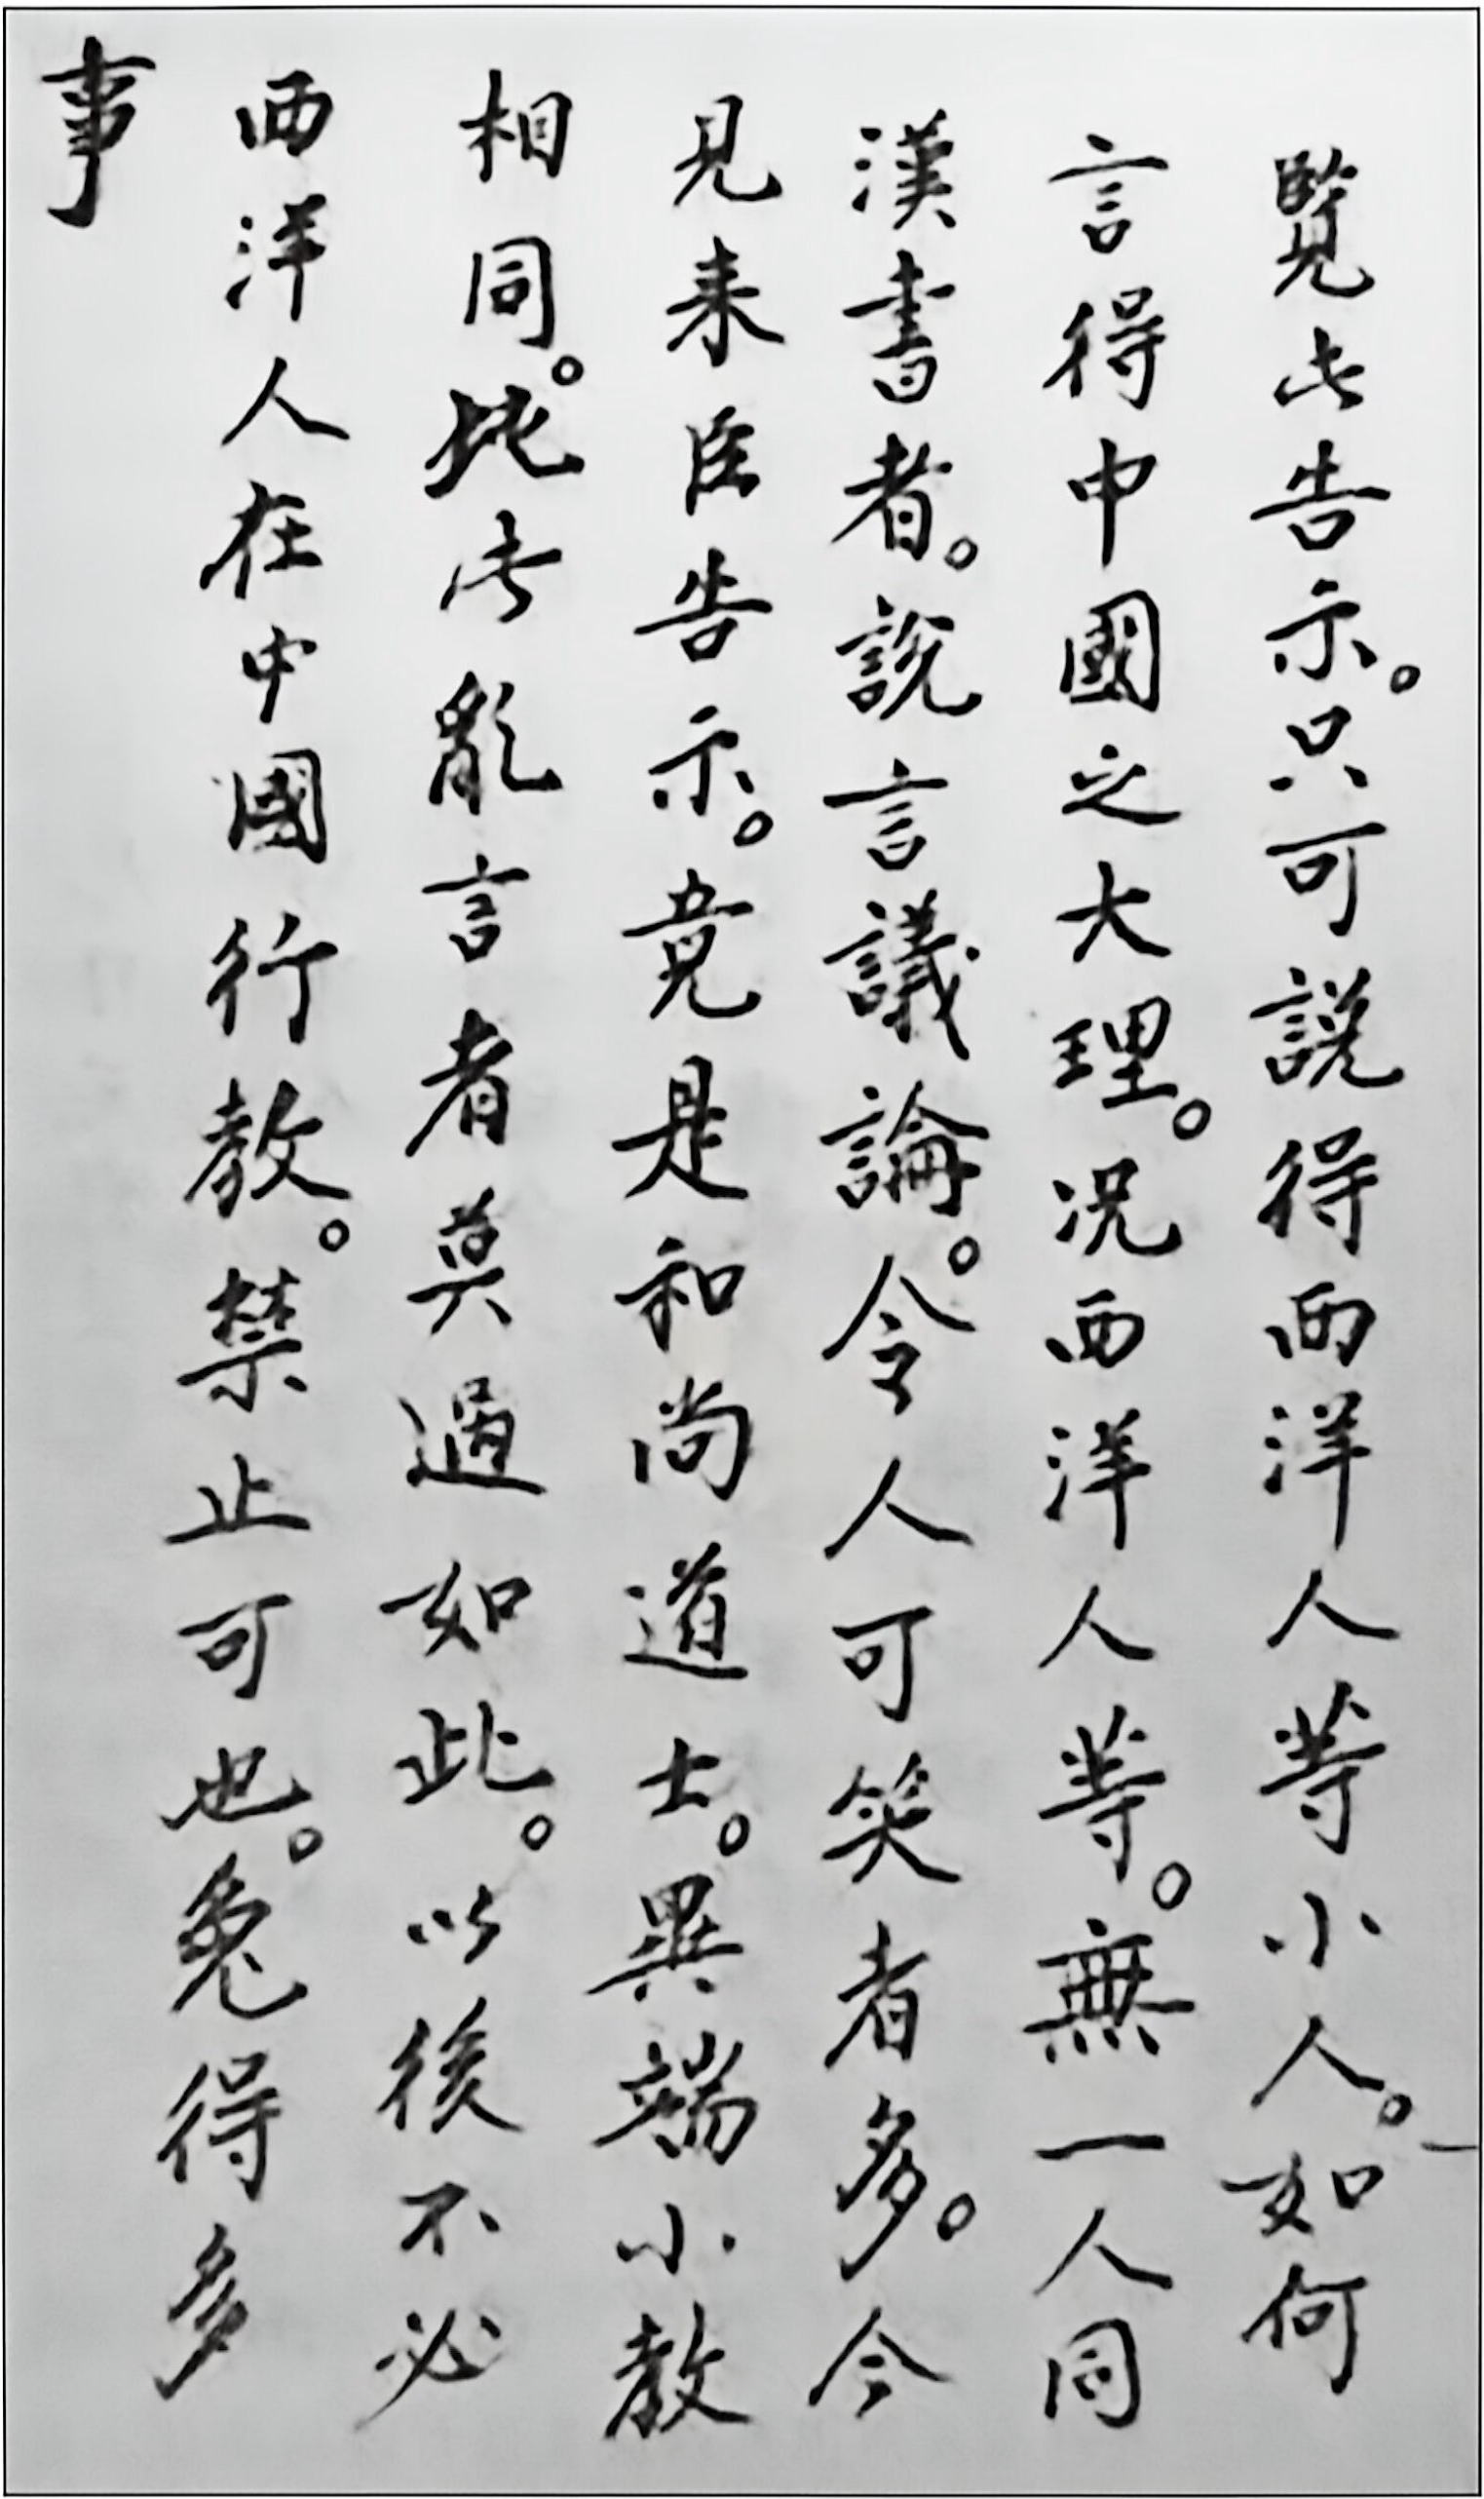
\includegraphics[width=\linewidth,height=.76\textheight,keepaspectratio]{assets/figures/kangxi-papal-decree.png}
\caption*{图6.1\quad 康熙批注教皇禁约}
\BookFloatNotes{图片来源：陈垣编，《康熙与罗马使节关系文书》，文件12。}
\end{figure}%
嘉乐在葡萄牙里斯本等待去中国船的时候，教皇确实派人给嘉乐送去%
了备选方案。\NoteRef{6}{83}这一点康熙应该事先不知道，不过他还是猜到了。%
\par
% 原书页码：238；段落
不出康熙所料，嘉乐收到康熙的批注和谕旨以后，很焦虑。第二%
天，他呈上了禁约的解说方案，写道“嘉乐来时，教王还付于臣条约%
解说一张”，请康熙过目。嘉乐给出的解说，就是对礼仪问题中一些%
活动给出了通融，总共有八条。\NoteRef{6}{84}八条如下：%
\par
% 原书页码：238；段落
{\bookkai 第一，中国基督徒在家中被允许使用上面仅仅刻着亡者名字的牌}%
{\bookkai 位，在这个牌位旁边必须附有一个基督徒对死亡的看法的恰切说明。}%
{\bookkai 立这块灵牌必须没有任何迷信的暗示，必须避免一切恶表。}%
\par
% 原书页码：238；段落
{\bookkai 第二，不是迷信的，也不会被怀疑为迷信的礼敬亡者的民间礼仪，}%
{\bookkai 可以得到准许。}%
\par
% 原书页码：238；段落
{\bookkai 第三，对孔子的民间性礼拜是准许的，也准许用牌位敬拜他，牌}%
{\bookkai 位上必须没有迷信的刻字，并且需要伴随着对天主教信仰的声明。同}%
{\bookkai 样，在修订过的牌位前准许点燃蜡烛、焚香和供设食品。}%
\par
% 原书页码：238；段落
{\bookkai 第四，允许在葬礼上使用蜡烛和香，但需张贴必要的声明。}%
\par
% 原书页码：238；段落
{\bookkai 第五，在修订好的牌位面前，以及棺木和亡者面前允许叩拜}%
{\bookkai 和匍伏敬拜。}%
\par
% 原书页码：238；段落
{\bookkai 第六，桌子上可以准备美味珍肴、水果、肉和其他按风俗习惯}%
{\bookkai 供给的食品，在灵柩前面或周围可以放置修订过的牌位。也必须作}%
{\bookkai 必要的声明，没有任何迷信的色彩。所有这些都是向亡者表示孝爱}%
{\bookkai 和尊敬。}%
\par
% 原书页码：238；段落
{\bookkai 第七，可以准许在中国新年和其他节期向着修订过的牌位叩头。}%
\par
% 原书页码：239；段落
{\bookkai 第八，在修订过的牌位前可以燃烛和焚香。在墓前也可以供设食}%
{\bookkai 品，只要采取上面提到过的预防措施即可。\NoteRef{6}{85}}{\bookkai 85}%
\par
% 原书页码：239；段落
康熙收到这八条通融条款以后，很满意。这变相同意了中国天主教徒%
参与很多之前被禁止参与的传统活动，要求是参与者自已发一个声明。%
尽管康熙还是让嘉乐把他关于中国礼仪的评论带回给教皇，但他马上%
全盘接受了通融条款。康熙早就看出天主教这个内部争议是扯不清楚%
的，同时也看出这八条通融条款确实做出了很大让步，教皇已经给足%
了他面子。他借着这个通融条款下了台阶，结束了这场争论，应该说%
对各方面都是最好的结果。%
\par
% 原书页码：239；段落
尽管在嘉乐拿出通融条款之前，康熙在谈判中的文字，以及给教%
皇禁约下的批注，处处透着他的威严和愤怒。但有意思的是，他收到%
嘉乐通融条款三天后，态度又变得和蔼可亲，气全都消了。他把所有%
北京传教士和嘉乐召集到一起，对嘉乐说：%
\par
% 原书页码：239；段落
{\bookkai 今节\AuthorNote{〔春节〕}近，尔于明岁再定回去日期。今事体俱已明白；朕}%
{\bookkai 之旨意，尔亦全晓。尔系使臣，辩论道理之时，朕必直言无隐。尔既}%
{\bookkai 不复争辩，朕仍前优待。朕原视中外为一家，不分彼此。尔可少息}%
{\bookkai 一二日，京城内天主堂，随尔便居住，以副朕怀柔至意。\NoteRef{6}{86}}%
\par
% 原书页码：239–240；段落（跨页续段）
康熙是在1721年1月21日向嘉乐说的这段话。从中可以看出，康熙%
已经完全不生气了，除了让嘉乐随便在京城教堂居住以外，还特别解%
释了为什么此前他的态度强硬，因为那是“辩论道理”，必须“直言%
无隐”。康熙大概觉得他之前话说得太重，把嘉乐给吓着了，所以有%
必要解释一下。\NoteRef{6}{87}%
\par
% 原书页码：240；段落
还有一个细节，特别值得注意。在给嘉乐禁约批注，威胁要禁%
教的那一天，康熙还命令隆科多去抓捕悄悄潜人北京的利国安神父%
（Giovanni Laureati，1666—1727）。利国安是罗马耶稣会派到中国的巡%
视官，主要责任是来督促北京耶稣会神父遵守教皇禁约的。他偷偷潜%
入北京，游说北京的耶稣会神父。康熙其实早就知道他的行踪，一直%
睁一只眼闭一只眼。不过在他决定亲自出面和嘉乐谈判时，就下令把%
利国安抓起来。隆科多当天在北京一座教堂的墓地抓到了利国安。康%
熙让隆科多把利国安带到嘉乐面前，当着嘉乐的面审问他为什么偷偷%
摸摸藏在墓地里面。%
\par
% 原书页码：240；段落
我们可以站在嘉乐的角度来思考当时的情况。在收到康熙威胁禁止%
天主教的当天，又看到了隆科多带着军队搜捕罗马耶稣会派到中国的巡视%
员。嘉乐当时面临的压力可想而知。还有一点要注意，嘉乐本质上是个神%
父，他并不是一个政治人物。他的一生除了这次出使中国，都是在教堂里%
做神父。当康熙用上各种政治手段，嘉乐是完全没有招架能力的。这也是%
为什么他第二天就把带来的通融条款全部交上去了。从康熙命令隆科多缉%
拿利国安的时间选择上来看，康熙当时是在打组合拳，一方面文字上施压，%
一方面行动上施压。当然康熙本来也只是吓唬一下嘉乐，抓捕利国安是“项%
庄舞剑，意在沛公”，收到嘉乐的通融条款后两天，就把利国安给放了。\NoteRef{6}{88}%
\par
% 原书页码：240–241；段落（跨页续段）
1721年1月28日是这一年的春节。嘉乐在北京过了春节，还参%
加了很多聚会。他也见到了当时在京的俄罗斯使团。整个1721年2月，%
嘉乐可以说都是在节日的气氛中吃喝玩乐度过的，收取各方礼物，同%
时也送出各种礼物。2月11日，嘉乐还参加了康熙举行的元宵节宴席，%
一直吃喝到晚上。2月18日，康熙把送给教皇和葡萄牙国王的礼物，%
交给了嘉乐。\NoteRef{6}{89}葡萄牙国王为了中国礼仪之争的事，几次派人到罗马%
规劝教皇。这些康熙是知道的，所以他专门准备了赠送葡萄牙国王的%
礼物。3月1日，康熙给嘉乐举行了高级别的告别仪式。\NoteRef{6}{90}这些谈判后%
的各个细节都显示，康熙对嘉乐的表现和谈判的结果是满意的。%
\par
% 原书页码：241；段落
嘉乐离开北京后，先到达广州，最后于1721年6月登船离开。嘉%
乐离开以后，康熙一直到1722年12月20日去世，还在继续盼望更多%
西洋人的到来。嘉乐走后不久，康熙让两广官员留意物色有技术的西洋%
人。1721年8月，广东巡抚就上报了来华西洋船，以及船上有技术的%
洋人。\NoteRef{6}{91}同时，康熙也没有忘记他派出去的使臣，最后装在棺材里运回%
来的艾若瑟。康熙从内务府里派人到广东，为艾若瑟修墓地。内务府为%
艾若瑟购买了37亩土地（超过三个足球场大小），其中10亩用来修墓%
地，27亩用来耕作，所得之钱用来维护墓地。从墓地购买的规模能看%
出康熙对艾若瑟很重视。墓地现在已经没有了，但是在鸦片战争以后，%
有英国人来拜访过这个墓地，记录了当时周围的环境，并全文抄录了%
墓碑上的文字。从碑文上可以知道，康熙给的艾若瑟名头是“钦差”。\NoteRef{6}{92}%
\par
% 原书页码：241；段落
墓志铭记录了艾若瑟的生平，主要强调他作为钦差，排除万难，%
一心回到中国复命的事迹。全篇写法大概学的是《汉书·苏武传》。%
从墓碑上的日期来看，墓地完工于1722年12月11号，也就是康熙%
去世前九天。同时，墓碑上的文字也说明康熙没有再追究艾若瑟滞留%
欧洲的原因，而是接受了教皇的说法：艾若瑟是因为身体原因没能及%
时回来。墓碑的残件现存于广州博物馆（图6.2，图6.3）。%
% 原书页码：242；图表（图题／表题所在页）
\begin{figure}[tbp]\phantomsection\label{fig-259-0}
\centering
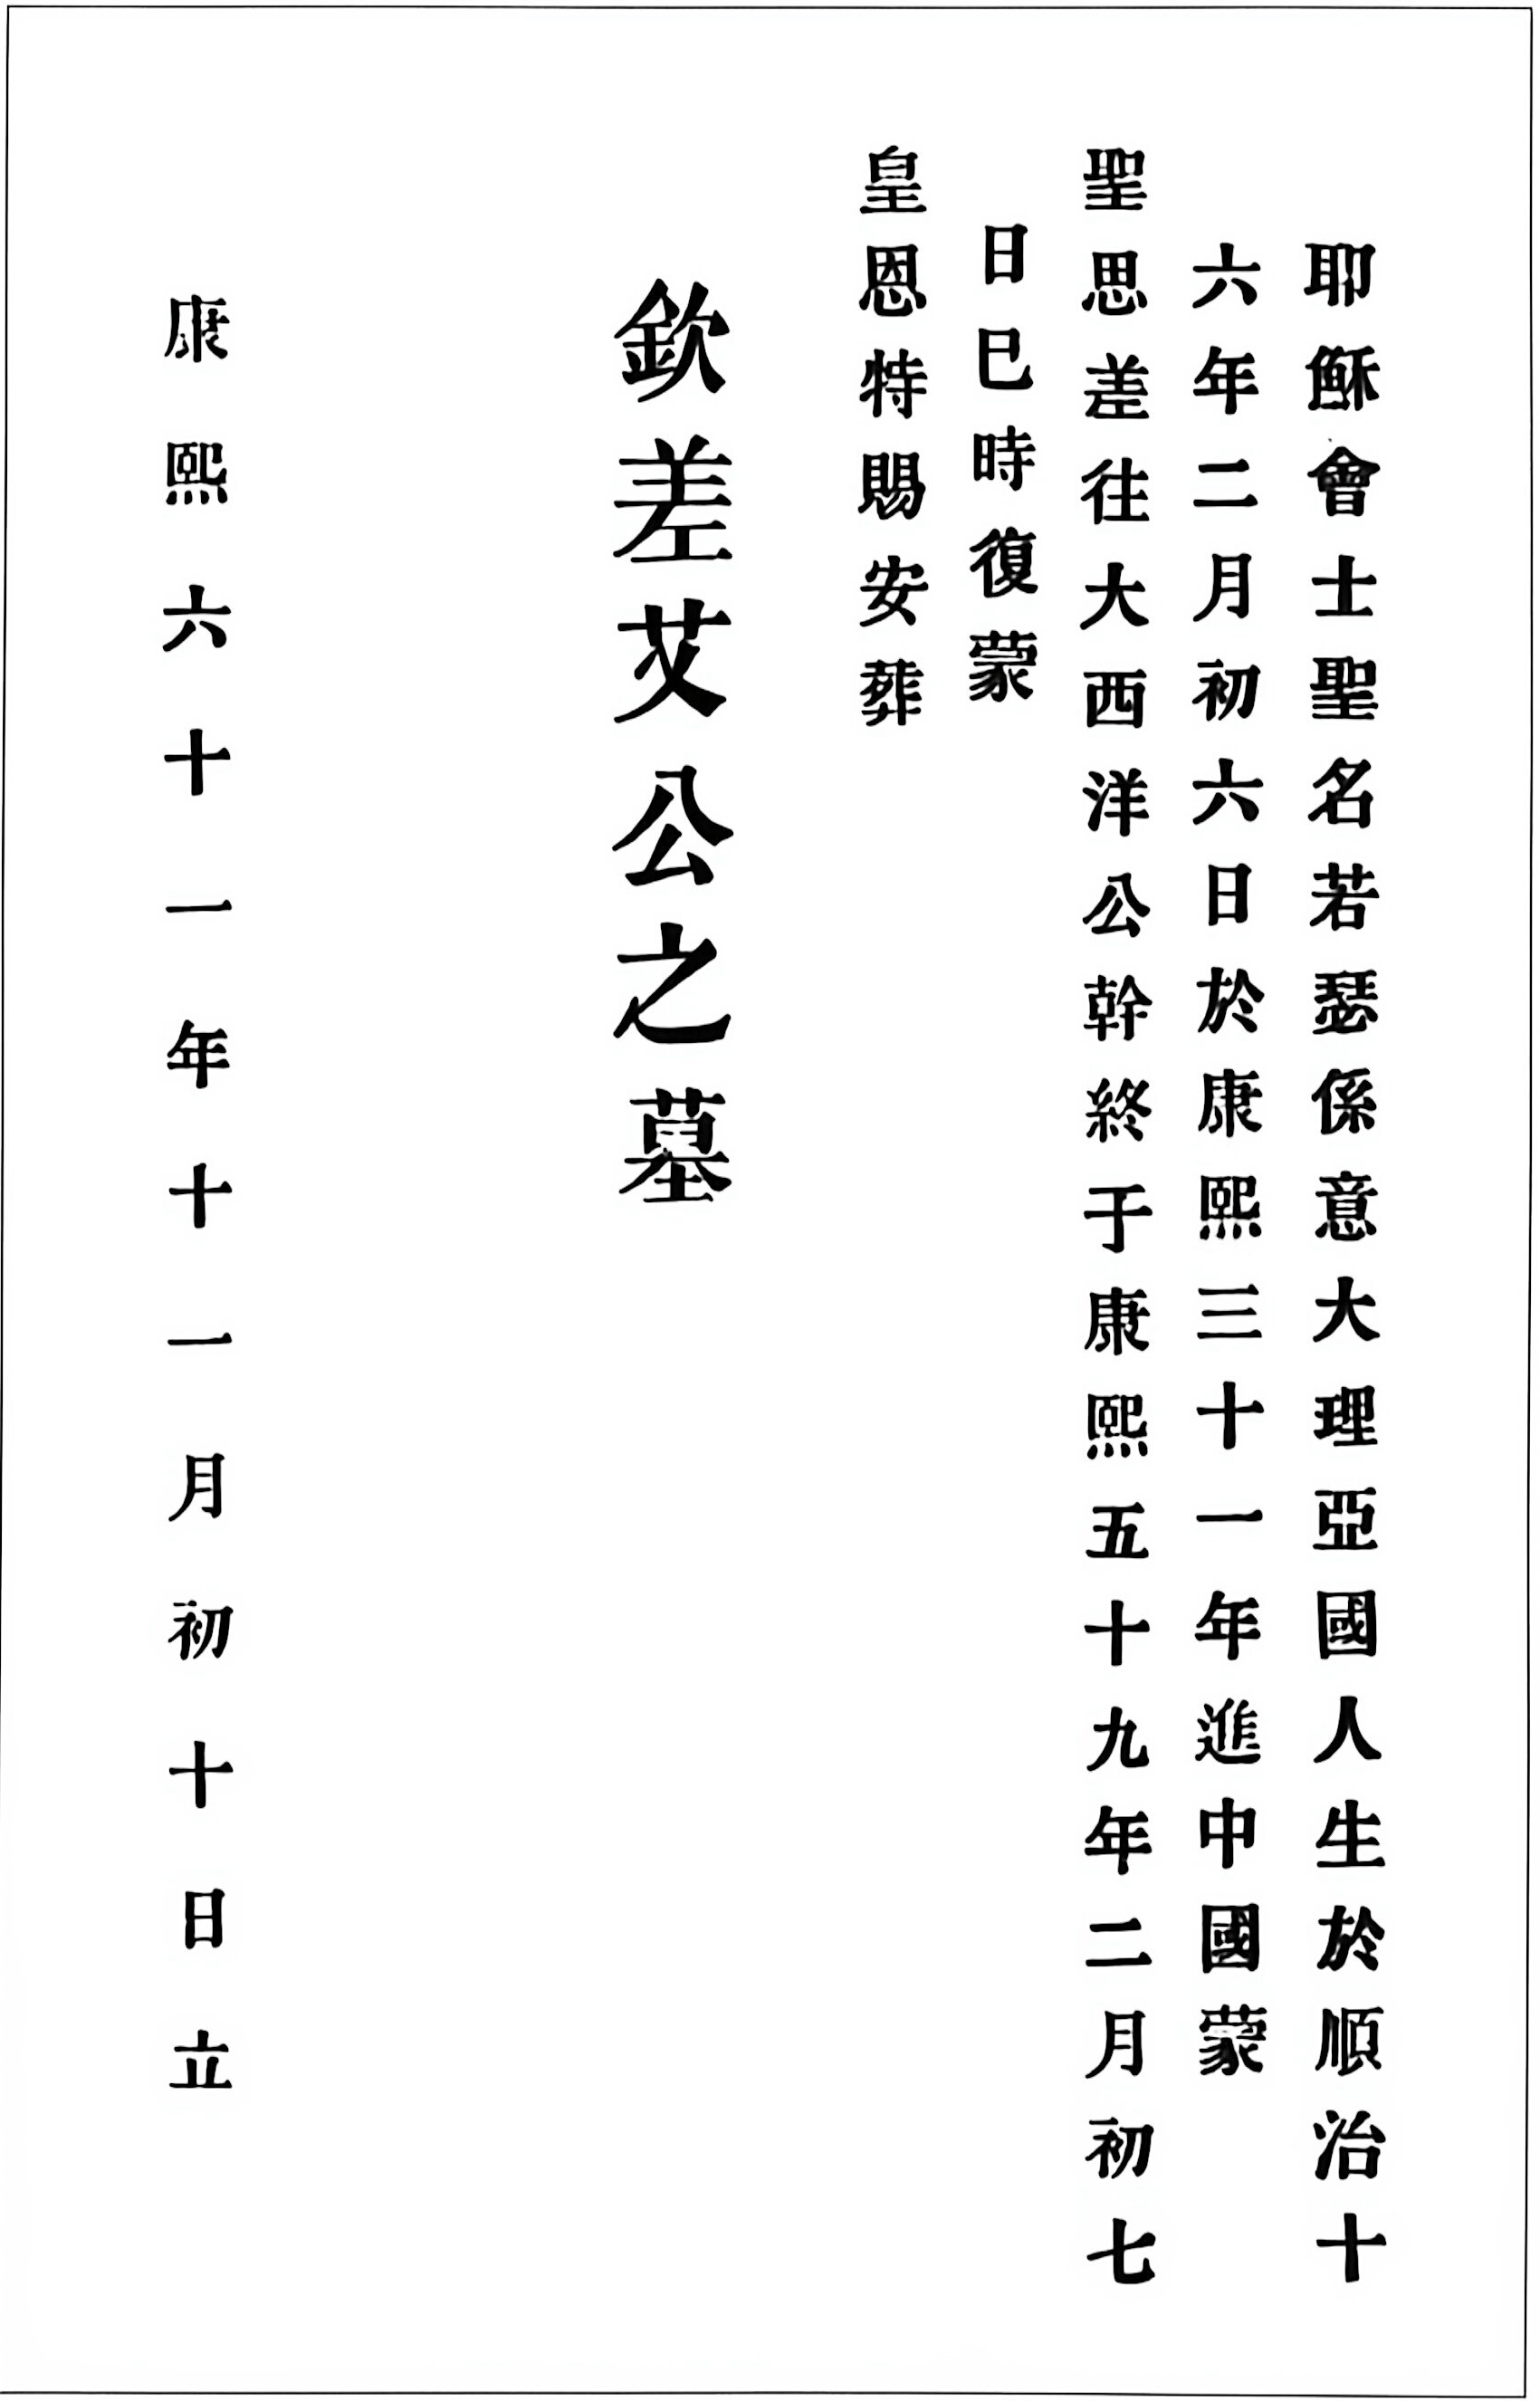
\includegraphics[width=\linewidth,height=.76\textheight,keepaspectratio]{assets/figures/suarez-tomb-front.png}
\caption*{图6.2\quad 艾若瑟墓碑正面碑文}
\BookFloatNotes{图片来源：Gray, John Henry. Walks In the City of Canton, 634.}
\end{figure}%
% 原书页码：243；图表（图题／表题所在页）
\begin{figure}[tbp]\phantomsection\label{fig-260-0}
\centering
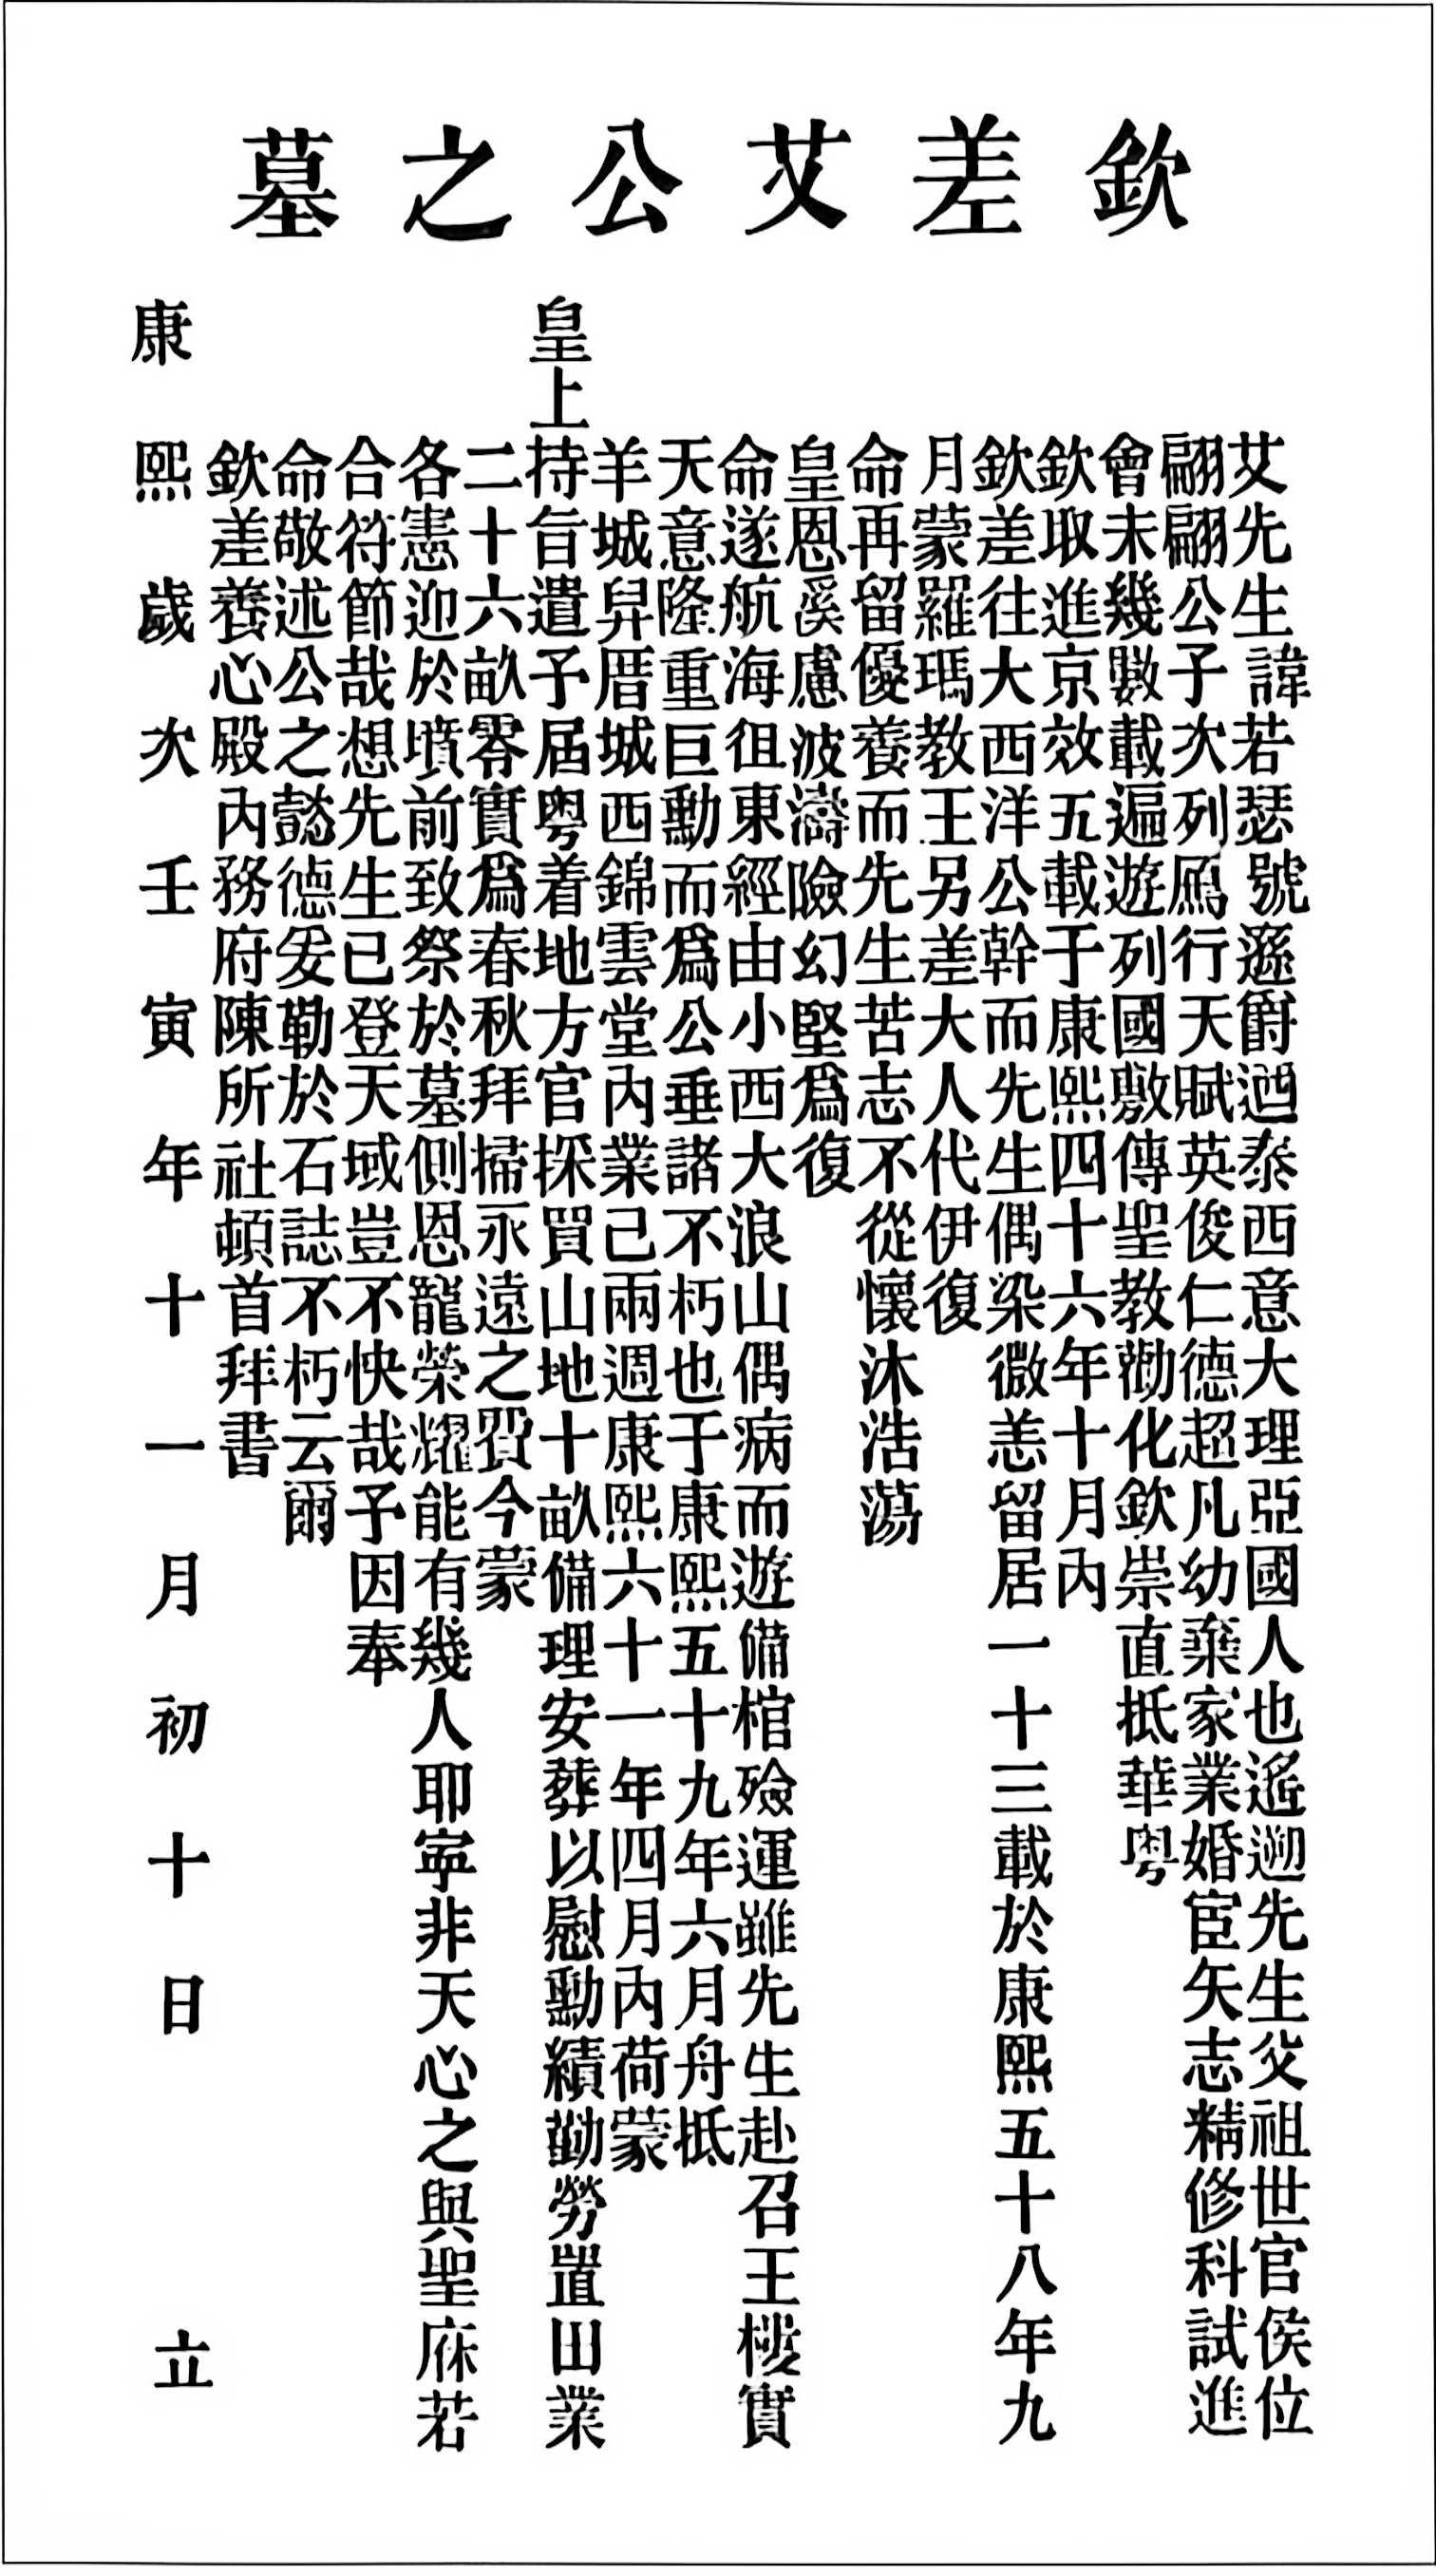
\includegraphics[width=\linewidth,height=.76\textheight,keepaspectratio]{assets/figures/suarez-tomb-back.png}
\caption*{图6.3\quad 艾若瑟墓碑背面碑文}
\BookFloatNotes{图片来源：Gray, John Henry. Walks in the City of Canton, 635.}
\end{figure}%
% 原书页码：244；标题
\subsection{小结}
\par
% 原书页码：244；段落
康熙从一开始就很清楚中国礼仪之争是罗马教会内部的争论。%
大清内部民族、宗教林立，康熙当然知道各种宗教内部的教义和规%
矩与传统中国的儒家文化有冲突。汉传佛教、藏传佛教和道教都有%
教规、戒律与儒家传统准则相违背。这并不是什么特别的事。在教%
皇的思维中，信仰是一个双向选择，信徒如果愿意遵从儒家的规则，%
那么他可以选择不信天主教。反过来，如果他们选择了相信天主教，%
就应该遵守天主教的教规。这一点是教皇给康熙写的信中最核心的%
一个观点。教皇反问“我们听说对其他宗教的信徒你们并不要求什%
么，也不过问他们是否遵守中国的礼仪习俗”，潜台词就是，您何必%
为难我们呢？这些道理康熙其实都明白，他参与天主教内部的争论%
并不是要坚持什么理论，而只是为了支持耶稣会神父，因为他们是%
他内务府的人，相当于自已的包衣奴才。按照满人传统，主子维护%
奴才，是不讲道理的。%
\par
% 原书页码：244–245；段落（跨页续段）
康熙最初没有想到这个礼仪问题会带来这么多麻烦。嘉乐拿出妥%
协的八条通融条款后，康熙借坡下驴，立刻就接受了，结束了这场漫%
长的争论。其实当时耶稣会神父对条款还不满意，但康熙这次没有继%
续听他们的了。根据马国贤神父记载，康熙对嘉乐说，他以后保证不%
会再介人他们宗教的内部事务了。\NoteRef{6}{93}所幸的是，最后双方对结果都满%
意。1721年春节，双方都在欢乐的气氛中度过了。嘉乐离开时，康熙%
和嘉乐都对未来双方进一步沟通交流充满了希望。历史也确实是这样%
在演进。嘉乐走后一年，康熙收到了罗马新继位的教皇英诺森十三世%
（Innocent XII）登基后专门发给康熙的通报。\NoteRef{6}{94}%
\par
% 原书页码：245；段落
那么为什么以前的历史，大多认为教皇的两个使团是失败的呢？%
这大概有两个原因。第一个是欧美历史研究中一直存在的欧洲中心%
论。站在欧洲人的角度，两次出使都没有达到他们要达到的结果，而%
是做出了很大的让步。在欧洲研究者眼中，妥协就是失败。1940年%
代，最早研究两次出使的学者安东尼奥·西斯托·罗索（Antonio Sisto%
\space%
Rosso），欧洲史料、汉文史料都看到了，也知道最后康熙和嘉乐达成%
了一致，可还是坚持嘉乐的第二次使团是继多罗使团后的“再次失%
败”，因为嘉乐没能够让教皇禁约完全在中国施行。\NoteRef{6}{95}这个欧洲中心论%
应该也是欧洲工业革命以后才有的论调。起码嘉乐回到欧洲时，教皇%
对结果是满意的，葡萄牙、法国等国家也都是满意的。在葡萄牙的帮%
助下，嘉乐还把教廷一直觉得有亏欠的多罗的遗体从澳门带回罗马安%
葬。嘉乐回去不久，也得到了教皇的嘉奖。所以欧洲中心论其实是后%
来的产物。当时，起码面对康熙，欧洲没觉得自己是中心。%
\par
% 原书页码：245；段落
第二个原因是对历史材料的误读。因为大清一方没有接待教皇使%
团的官方记载。1930年代发现的原始材料是没有背景的历史档案。如%
果对历史脉络没有完整了解，就只能看到字面意思。比如，本章提到%
关于康熙威胁要禁止天主教的话，这种在谈判中说的重话、狠话，不%
能只看表面意思，应该具体判断。%
\par
% 原书页码：245–246；段落（跨页续段）
另外，康熙当时能从容应对世界各地来的使团，很重要的一个因%
素是他有能力绕开整个朝廷制度。他1720年接待的彼得大帝使团和教%
皇使团在正史中都没有记载。为了谈判需要，康熙通过内务府把接待%
教皇使团的关键过程都记录下来。记录的方式类似于今天的会议摘要。%
康熙派传教士找到俄罗斯使团，让他们帮忙把会议记录带回了欧洲。\NoteRef{6}{96}%
这份记录在民国时期整理故宫档案时由陈垣在康熙的书房懋勤殿中发%
现。尽管有这份记录，但是似乎大清的历代史官都没有看到过。雍正、%
乾隆朝编撰的各种官方史书都不知道教皇在康熙年间就派了两个使团%
到中国，而是一直以为教皇的第一个使团是雍正年间才人华的。\NoteRef{6}{97}%
\par
% 原书页码：246；段落
最后，有一点值得强调，尽管中国礼仪争论看似是关于中国礼仪%
问题，但这个问题的辩论场主要在欧洲。康熙多少给出了他的看法，%
算是参与到争论中，但他并没有把这个问题扩大。所以当时大清的儒%
学大师和高官基本没有参与争论。“中国礼仪之争”准确来说是欧洲教%
廷内部的一个问题，而不是中国的一个社会问题。如果说天主教的“中%
国礼仪之争”对中国完全没有影响这一说法有点绝对的话，那么说礼%
仪之争影响了天主教在中国的历史轨迹肯定就言重了。后来还有说礼%
仪之争引起了后来的雍正禁教，那就更是无稽之谈了。那么到底为什%
么雍正登位就要禁教呢？且看下章分解。%

\clearpage\markboth{第三部分\quad 荣耀后的沉寂}{第三部分\quad 荣耀后的沉寂}
% 第三部分 荣耀后的沉寂
% 原书页码：无印刷页码；标题
\part{荣耀后的沉寂}

\clearpage\markboth{第七章\quad 雍正争位与禁教}{第七章\quad 雍正争位与禁教}
% 第七章 雍正争位与禁教
% 原书页码：249；标题
\section{雍正争位与禁教}
\par
% 原书页码：249；段落
雍正五年四月初八（1727年5月24日），雍正收到了广东发来的%
消息，新来的葡萄牙使团已经离开广东赶来北京了。这一天正好是释%
迦牟尼佛的生日，雍正在朝会上公开评论了天主教和佛教：%
\par
% 原书页码：249；段落
{\bookkai 今日为佛诞之期，恰遇西洋国使臣上表称贺，两事适然相值，尔}%
{\bookkai 等在廷诸臣奏事之暇，偶将朕意宣谕尔等知之。……朕意西洋立教之}%
{\bookkai 初，其人为本国所敬信或者尊之如天。倘谓立教之人，居然自称为天}%
{\bookkai 主，此理之所无者也。释氏原以清净无为为本，以明心见性为功，所}%
{\bookkai 以自修自全之道，莫善于此。\NoteRef{7}{1}}%
\par
% 原书页码：249–250；段落（跨页续段）
雍正在朝会上公开对着群臣臧否宗教，是很少见的，特别是他评点的%
内容和时政又没有什么关系。雍正大概也知道这有点不合常规，所以%
还专门解释了一下，他只是在大臣们“奏事之暇”，抽时间说几句。%
很明显，雍正这段话说明他对天主教中像“天主”这样最基本的概念%
都是不认同的。尽管他措词委婉，“此理之所无者也”，但明白人都能%
听出，雍正是从根本上否定了天主教。同时，雍正也讲出了他心中最%
好的宗教，那就是释氏的佛教。在朝堂上，面对朝臣，这样公开的一%
贬一褒，雍正的态度不能再明确了。%
\par
% 原书页码：250；段落
其实，早在三年以前，雍正元年都还没过完，他就废除了康熙的%
容教诏令，禁止传教士在中国地方上继续传教。传教士只能留在京城%
为朝廷做天文观测这样的技术性工作。当然，北京的传教士也没闲着。%
从雍正禁教起，他们就在北京找各种关系，希望说服雍正取消禁令。%
雍正也明白这个在路上的葡萄牙使团，大概又是来求情的。在葡萄牙%
使团来华前两年，雍正已经拒绝过教皇派来的使团。\NoteRef{7}{2}所以雍正在收到%
葡萄牙公文以后，就在朝堂上公开评价了天主教，并让官员们把他的%
意思带给葡萄牙使团。%
\par
% 原书页码：250–251；段落（跨页续段）
北京传教士烦恼的不仅仅是他们的宗教这样被皇帝公开羞辱，%
最让他们沮丧的是他们看不到一点儿希望。康熙去世后，他们在北%
京的状况江河日下，一步步被排挤出了北京的权贵圈。雍正登基后，%
第一件事就是把他自己府上的和信任的人，换去管理内务府。传教%
士作为康熙内务府的一部分，与康熙其他近身奴才遭遇基本一样，%
都被逐出了宫，不再属于内务府。据马国贤神父回忆录所记，雍正%
元年管理内务府的是康熙的十七皇子，他把神父们召集到一起，通%
知他们以后就不再归内务府管，也不算内务府的人了。不归内务府%
管也就是被剥夺了内务府身份，最直接的一个结果就是以后他们得%
不到皇帝的专门召见，不能人宫了。皇十七子还专门强调了这一点。\NoteRef{7}{3}%
能入宫面圣是了不起的特权。这个传教士享有了超过半个世纪的特%
权，就这样被取消了。最让传教士们失望的是，雍正皇帝连表现机%
会都没有给过他们，就直接把他们赶出了内务府。没有了内务府的%
身份，他们就只是一群懂天象观测的术士，地位一下子就跟市场上%
掐八字算卦的没多大区别了。%
\par
% 原书页码：251；段落
从被赶出内务府，到雍正全面禁止天主教，中间大概相隔了九个%
月时间。这期间，传教士已从朝野上下对他们态度的转变中，预感到%
了禁教的前景。被逐出内务府对传教士来说是釜底抽薪，一下断了他%
们在大清朝野存在的根本，朝野上下也都明白这其中的意味。传教士%
很真切地感受到了各方面势力对他们态度的变化。很快，许多权贵都%
开始回避他们，不和他们来往了。%
\par
% 原书页码：251；段落
雍正继位的时候已经四十五岁，思想、性格都已经完全成熟。对%
于传教士来说，他们没有任何机会影响、改变雍正。这一点，跟当年%
七岁继位的康熙不一样。传教士那时接触到的康熙，正处在学习阶段。%
他们成功地用他们的知识来引导康熙，让康熙对西洋知识、器物都发%
生了兴趣。可惜的是传教士的一切在雍正那里都没有吸引力。雍正%
二十岁开始就喜欢和喇嘛、和尚、道士往来。在雍正还是皇子的时候，%
传教士也没有特别花过功夫去接近雍正，双方尽管没有矛盾，但也没%
有特别的关系。前章讲到，传教士在康熙朝受到的厚待得益于他们和%
康熙之间的关系，那么雍正朝他们受到的冷遇，也是他们和雍正关系%
的体现。传教士和康熙各个皇子建立关系的黄金时段是康熙晚年废掉%
太子以后，也就是康熙的最后十年。在这段时间里，为什么传教士会%
错过雍正，没有和他建立起良好的关系呢？这就不得不说到康熙晚年%
的储位斗争。%
% 原书页码：252；标题
\subsection{康熙晚年的皇位争斗}
\par
% 原书页码：252–253；段落（跨页续段）
康熙晚年的储位之争大概是他一生中最感棘手的问题。涉及的人%
都是自己的儿子和亲人，手心手背都是肉，康熙很难恰到好处地处理。%
满人的传统，大多是不立太子的。努尔哈赤和皇太极去世的时候，都%
没有立太子。但也正是因为没有立太子，二人死后满人内部都有剑拔%
弩张的争位戏码上演。立太子是汉人朝廷的传统，也是皇位和平有序%
传递的一个措施。1675年，康熙听了汉人臣子的意见，在他二十一岁%
的时候，就册立了当时才两岁的皇二子为太子。太子长大后，中年的%
康熙也确实体会到了立太子的好处。康熙几次塞外远征和南巡，都是%
太子坐镇北京，管理朝廷日常运作，让康熙可以放心远走。但问题是，%
康熙走后，太子在北京朝廷中体验着当皇帝的感觉，康熙回来，他又%
回到太子的角色上去。太子等待皇位的时间是漫长的，在当了三十三%
年的太子以后，还是在1708年被废了。康熙在颁布的废太子诏中，%
从太子“秉性乖戾”说起，给出了一大堆太子不好的理由。不过，最%
本质的问题应该还是康熙察觉到了太子想登位，他自己感受到了威胁。%
但是废黜太子并不是解决皇储问题的办法。康熙很快发现这一举动反%
而激化了皇储问题中隐藏的各种矛盾。太子位空缺让他众多儿子看到%
了机会，一个个蠢蠢欲动，同时整个朝廷的各派势力也通过支持不同%
的皇子在暗中角力。康熙的大皇子甚至对康熙说，如果杀废太子下不%
了手，他可以出手。康熙一直敬重的舅舅佟国维推荐立皇八子为太子，%
康熙不同意，也让舅舅不要掺和这事。佟国维则直言康熙要让自己闭%
嘴的话，除非把自己给杀了。遇到这种家务事，舅舅又这样讲话，康%
熙应该是很烦恼的。历史记载中他和舅舅佟国维的争论只是只言片语，%
但从后来康熙的反应看，二人应该不是简单的几句争吵而已。康熙幼%
年就丧父丧母，他小时候，母亲家里的两个舅舅佟国纲、佟国维一直%
作为侍卫守在他身旁。他们之间是有深切亲情的。传教士记录中，康%
熙无论朝堂上还是私下里，都是亲切地直呼二人为“舅舅”。而佟国%
纲又在跟随康熙追击噶尔丹时战死疆场，佟国维就是康熙晚年最亲的%
长辈了。按正常情况，佟国维1719年去世，康熙会赐给他这个舅舅%
很高规格的葬礼。但实际上，康熙连谥号都没有给他。最后佟国维能%
有谥号，全靠他的儿子隆科多辅佐雍正有功。雍正上台第一年为了拉%
拢隆科多，就先给佟国维补上了谥号。这说明康熙晚年和他的舅舅为%
储位问题应该产生过很大的分歧。%
\par
% 原书页码：253；段落
康熙废黜太子不久，便发现太子身上的许多问题其实是大皇子从%
中搞鬼的缘故。这让康熙对废太子的决定有些后悔。权衡各种利弊之%
后，康熙又在一年后，也就是1709年复立了太子，希望以此结束皇%
储的纷争。太子尽管恢复了，康熙对太子的猜疑还是没法去除。康熙%
本来有南巡的雅兴，1699年、1703年、1705年、1707年数次南下，%
但经过1708年、1709年废太子后又复立太子，康熙至死都再没有长%
时间远离北京南下巡游。1712年，康熙再次废太子，公开的理由还是%
跟第一次废太子时差不多，就是太子品行等各方面都不配做一个君主。%
废太子一直被软禁，直到雍正登基后的第二年去世。康熙废太子以后，%
拒绝了所有立太子的建议，这也就开启了历史中被津津乐道的九子夺%
嫡时期。%
\par
% 原书页码：254；段落
北京传教士既是康熙宫内人事起伏的见证者也是参与者。1675%
年，当两岁的太子刚刚被立以后，传教士就开始了长远计划，努力%
接近太子和他的势力圈。这个圈子的核心是索额图，是太子母亲的%
叔父。传教士一直和索额图保持着密切的私人关系。很多传教士的%
书信中都提到过索额图，称他为“索三”，因为他是索尼家的第三子。%
索额图和传教士的往来在铲除鳌拜之前就开始了。传教士能得到康%
熙颁布的容教诏令，就是索额图帮传教士打通了礼部的各个关节。%
有了索额图的这层关系，传教士在太子还未成年之时就在太子的核%
心圈子中了。从北京传教士发回欧洲的信中可以看出，他们对太子%
赞誉有加，而且认为他能延续康熙的容教政策。1706年，教皇特使%
多罗参加了康熙的辞别会后，还去了太子那边。多罗对太子的印象%
很好，认为太子会继续容留天主教。\NoteRef{7}{4}对传教士来说，1712年太子再%
次被废也是他们的重大损失，这意味着他们三十多年来在太子身上%
付出的心血付之东流了。他们需要重新猜测谁会是新的皇帝，并和%
可能的人选建立关系。%
\par
% 原书页码：254；段落
康熙一朝，传教士前后来去已历三代。他们跟所有的皇子都有交%
集。康熙学习了西方知识以后，让传教士把许多西学科目首先翻译成%
了满文，教他的儿子和皇族子弟。在康熙晚年争位的儿子中，大概可%
以分为四派：%
\par
% 原书页码：254；段落
第一派是废太子一派，以前的太子党还在寄希望废太子能有再被%
复立的一天。%
\par
% 原书页码：254–255；段落（跨页续段）
第二派是以皇三子为中心的一派。皇三子以学问大闻名，康熙把%
跟学问相关的项目都交给皇三子去办。比如著名的《古今图书集成》%
就是皇三子在主持。还有跟西学相关的天文、数学等项目也是他在负%
责。皇三子自已就是有学识的，他带着一帮满人子弟，通过他们自己%
的天文观测数据，竟然发现了传教士所讲天文学中的漏洞。在1716年%
前后，皇三子、十五子、十六子一起上书康熙，报告根据他们从1714%
年开始持续三年对夜晚的观测，发现传教士讲的天文理论有问题，有%
误差。\NoteRef{7}{5}对于皇子们发现的问题，传教士是承认的，只是说他们给的数%
据是目前最好的数据。有新来的传教士，康熙也是派皇三子去测试来%
者是否有真学问。在欧洲大学讲授数学的耶稣会传教士戴进贤来到北%
京，康熙就是派皇三子去测试的。\NoteRef{7}{6}%
\par
% 原书页码：255；段落
皇三子在以前争位历史中被提到的不多，但是皇三子在当时是一%
个不可小视的存在。研究雍正皇帝的学者黄培就提出，康熙最中意的%
皇子是皇三子，因为根据已知康熙晚年的满汉奏折来看，康熙联系最%
频繁、交办事务最多的皇子就是皇三子。\NoteRef{7}{7}后来雍正登位以后，第一年%
就把皇三子放逐去为康熙守陵，这也反映出雍正对皇三子的忌惮。康%
熙是否有心传位于皇三子，已无从考证。这里要强调的是，研读历史%
必须要站到当时人的环境中去体会。当时所有的人，包括传教士，都%
不知道康熙会传位给谁，他们只能猜测。那么他们猜测的凭据是什%
么？很重要的一点，就是看康熙把重要的任务交给哪个皇子，平时和%
哪个皇子走得近，往来的多。从这一点看，皇三子确实和康熙来往频%
繁。从现存的满文奏折上看，就特别明显。皇三子管着大大小小很多%
事，经常出现在奏折中。%
\par
% 原书页码：255–256；段落（跨页续段）
争位中第三派势力是各种史书、小说、电影、电视都经常提到的%
皇八子一系。这一派还包括皇九子、皇十子和皇十四子。在1708年%
废太子以后，皇八子确实有很高的呼声。八旗中支持皇八子的权贵众%
多，他在皇子内部也呼声很高。康熙的舅舅佟国维就支持皇八子。后%
来朝臣发现康熙铁了心不会传位皇八子，又把目光集中在这一派中的%
皇十四子。各种野史中盛传康熙有意传位给皇十四子的说法，并非空%
穴来风。康熙在晚年把最重要的西北军务交给了皇十四子。康熙一生%
最在意的就是平定西北，消灭还没有归顺的蒙古部落。皇十四子有勇%
有谋，在处理青海、西藏等问题上让康熙很满意。只是皇十四子在西%
北的历史功绩后来在历史中被雍正抹去了。%
\par
% 原书页码：256；段落
康熙晚年，皇子内部就认为康熙让皇十四子领兵去西北，就说明%
他有意把皇位给皇十四子，同时也用这个任务来最后考察皇十四子。%
对于这一点，当时人应该都知道。传教士穆经远被抓以后的审讯记录%
里面提到这事。穆经远承认他确实听到过皇子之间说康熙让皇十四子%
领兵就是中意他的表现。\NoteRef{7}{8}%
\par
% 原书页码：256；段落
同时，约翰·贝尔在他的记录中提到，他当时在北京听说，皇位%
是要传给皇十四子，同时也说皇十四子正在处理当时最麻烦的西北军%
务问题。约翰·贝尔所在的彼得大帝使团是1721年3月离开北京的，%
也就是在康熙去世前大概一年半时间。他这条记录应该算是一个跟大%
清内部没有任何利益关联的人留下的一条珍贵的历史记录。\NoteRef{7}{9}争夺皇位%
的历史情形复杂，这里只能讲到一个脉络。就本书关注的传教士来说，%
他们也跟众多朝臣一样，把宝押在了这一派上。%
\par
% 原书页码：256–257；段落（跨页续段）
第四派就是最后登位的雍正一派。雍正一派中还有皇十三子，这%
也是历史中常常提到的人物。在上面四派中，传教士可以说跟前面三%
派都有很好的关系。唯独在皇四子雍正这里，传教士基本没有下过功%
夫。为什么在废太子以后漫长的十年中他们会恰好错过雍正？要真正%
理解这个问题，必须站在传教士的角度思考。站在传教士角度最重要%
的一条，就是要明白他们是历史中的人物，无法知道历史后来的演进，%
不知道最后皇四子会登位。他们所有的决定，都是基于他们当时所观%
所感，做出他们认为的最好选择。%
% 原书页码：257；标题
\subsection{雍正登位中的谜团}
\par
% 原书页码：257；段落
康熙是1722年冬在京郊打猎时染了风寒，突然过世的。根据传教%
士记录，康熙其实在前一年身体不佳，而1722年身体已经恢复。康%
熙1722年秋已经去热河木兰打过一次猎了，冬天这次是再次出京打%
猎。这么频繁围猎也说明康熙身体没有什么问题，起码他自已没有感%
觉到有什么问题。所以康熙并没有特别准备过传位事宜，只是身体抱%
恙以后，在病床上匆忙开始了继承人选择。根据清史官方说法，康熙%
是口谕传位给皇四子的，给出的理由是皇四子“人品贵重，深肖朕躬”，%
就是说雍正品行好，康熙认为他像自己。正史中还说，传位时还有康%
熙的几位皇子和九门提督隆科多在场。%
\par
% 原书页码：257–258；段落（跨页续段）
从官方史料记载来看，传位皇四子并没有什么疑问，但雍正篡位%
的说法一直存在。这个说法到清朝灭亡，所有宫廷文档公开以后，变%
得更盛行。尽管没有铁证，但疑点很多。通过各种清官方记录比对，%
学者发现雍正时期删除了许多康熙时期的记录，而且删除的记录正好%
跟雍正的继位有关联。民国初年清史学者孟森对雍正继位的合法性做%
过深人考证，其中提到一点怀疑，这一点也是雍正朝时就被提出的问%
题：为什么雍正两个最亲的人，都对他登位不满？这两个人一个是雍%
正的母亲，一个是皇十四子。就宫廷常态来说，皇帝儿子众多，皇子%
之间一般最亲近的是同父同母的兄弟。雍正和皇十四子就是同父同母。%
在康熙驾崩之时，皇十四子正在西北处理西藏事务，过了几个月才回%
来，回来后就和雍正闹翻了，被雍正发配到城外居住。更诡异的是，%
雍正的母亲也对雍正继位没有半点高兴的样子，在雍正把皇十四子发%
配到城外以后，雍正的母亲竟然以死抗争，撞柱而死。这个“撞柱而%
死”当然在正史中不会说到，提出这个的是雍正时代的曾静。他列举%
了雍正十大罪状，游说川陕总督岳钟琪谋反，其中一条就是雍正逼死%
生母，是大不孝。至于雍正生母是否真像曾静所写是撞柱而死已不可%
知，但雍正生母对雍正登位不满，和雍正关系很差，这在很多历史记%
录中都能看到。所以为什么雍正当皇帝，连他母亲和亲兄弟都不满？%
这不得不说是一个很大的疑点。对于曾静的指控，雍正曾经公开逐条%
批判。雍正把逐条批判，以及曾静被抓后写的悔过书，一起结集出版，%
取名《大义觉迷录》。雍正这样一条条批判，相当于把当年的各种传言，%
以及宫廷矛盾记录下来，公布于众。但问题是雍正写的东西并没有起%
到他想要的效果，反而暴露出更多的疑点。因为他的记录又和当时其%
他正史记录有出人。%
\par
% 原书页码：258–259；段落（跨页续段）
乾隆初年，为了永远平息相关争议，乾隆又花大力气在全国范围%
内收回销毁了这本书。清末留日学生在日本发现了这本书，使其重见%
天日。\NoteRef{7}{10}孟森先生的考证很多就取自《大义觉迷录》，指出了很多细%
节与公布的正史之间的矛盾。\NoteRef{7}{11}后世怀疑的逻辑总结起来就是：如果%
继位没有问题，为什么会有那么多细节上的出入？而且是在雍正的御%
用学者编辑校对了正史各种记录以后，都还有那么多出人。也正因为%
存在各种疑点，雍正的继位问题成为后世每一位研究雍正历史的学者%
都绕不开的问题。当然这些疑点也为后世各种文学创作留下了想象的%
空间。%
\par
% 原书页码：259–260；段落（跨页续段）
了解了雍正继位的疑点，也才能理解传教士在雍正继位之前的%
言行。第一，传教士跟当时大多数的朝臣一样，并没有预测到雍正%
能够继位。这也是为什么传教士在雍正继位之前并没有专门花精力%
接近雍正，跟雍正私下建立起关系的原因。传教士内部其实分析过%
谁有可能继位，但他们并没有想到雍正。他们也跟当时的主流分析%
一样，把重心放在了皇八子和皇十四子一派上。当时，皇九子、皇%
十子在京城负责给在西北的皇十四子通报朝廷中的讯息。而传教士%
穆经远就属于皇九子一系，参与了康熙晚年皇子间的争位斗争。清%
亡以后，民国年间，雍正上位后处置皇八子允禩和皇九子允禟一派%
的案子就是当时的研究热点。当时故宫博物院把宫中发现跟案件相%
关的审问材料结集出版，取名为《允禩允禟案》。其中的第一份口供%
材料就是穆经远在雍正初年被抓以后录的。\NoteRef{7}{12}在罗马还存有一份当年%
刑部根据口供写的中文判决书（见附录四：穆经远判决书）。\NoteRef{7}{13}口供中%
他坦然承认和皇九子的密切关系，开头就说，皇九子对他好，是“天%
下共知”的。皇九子被雍正流放，穆经远就跟着他。单看口供，根%
本看不出他是一个西洋神父，反而处处显示出他是一个忠于主子的%
满人奴才。录口供的人还问穆经远，抓你的那天，你对着皇九子的%
房子跪地磕头是什么意思？这些如果还是小细节的话，那么穆经远%
口供里还说，他在康熙末年私自联系过年羹尧，给年羹尧送过礼物，%
这就是大事了。穆经远在康熙晚年还向康熙推荐立皇九子为嗣，当%
然这被康熙呵斥了，说他不懂规矩。这些事情都说明传教士是参与%
到了康熙晚年皇子夺位政治中的，他们心中有支持的候选人。不过%
可惜的是，他们的候选人没能登上大位。%
\par
% 原书页码：260–261；段落（跨页续段）
雍正的继位出乎朝廷上下意料，加上当时还有各种对他继位的流%
言，这些决定了雍正继位头几年的重点任务是逐步清除异己。雍正继%
位后的第一步就是更换内务府里面的人。那些常年跟在康熙身边的奴%
才都被换掉了。赵昌是康熙身边一个重要的贴身奴才。很多奏折上都%
能看到他的名字（注意赵昌是满人中的包衣奴才，不是太监，康熙还%
在其生病时，劝他禁房事）。传教士和他的私人关系也很好。雍正登基%
后，赵昌就被赶出宫，关在一个监狱里面。\NoteRef{7}{14}所以传教士们被赶出内%
务府，其实也不是雍正专门针对传教士的措施，只是雍正重新配置内%
务府人员的一个操作。后来乾隆上台以后，也把内务府里雍正养的和%
尚道士驱逐出宫，并且警告他们出去后不要乱说话。内务府就是管理%
皇帝家务事的部门，皇帝上任后，这里面的好多人物都要置换，属于%
常规操作。雍正朝由于有继位风波，外加雍正疑心大，当时被赶出内%
务府的人很多。内务府调整完后，雍正的第二步就是处理让他感到威%
胁的众兄弟们。雍正1722年冬继位，几个月后，就把皇三子发配去%
给康熙守墓，把皇九子发配到西宁，皇十子被移送到蒙古。皇十四子%
在康熙死后几个月赶回北京后，被要求在北京城外居住。当时皇八子%
在京城势力很大，人脉很广，雍正暂时没有动他，反而任用了他。雍%
正稳住大局后，在雍正四年正月把皇八子圈禁于宗人府，当年10月%
皇八子就死了。到皇八子死为止，可以说雍正前四年的执政重点都在%
打击异己、巩固皇位上。\NoteRef{7}{15}雍正和康熙以及后来的乾隆不一样，他在%
位期间没有长期离开过北京，也从来没有下过江南。雍正似乎对他的%
江山一直到死都有几分不安心。%
% 原书页码：261；标题
\subsection{传教士也尽力了}
\par
% 原书页码：261；段落
雍正元年秋（1723年10月），闽浙总督满保上了个折子，细数天%
主教在福建的问题，建议全国禁教。这个折子从内容上看，并没有多%
少新意，还是老生常谈，总体就是说天主教教义与传统观念有诸多冲%
突，不适合在中国传播等等。折子建议除有技术的北京传教士继续在%
朝廷留用以外，地方各省都应该禁止传教士出入传教。%
\par
% 原书页码：261；段落
这封奏折很简短，两三句说了地方上的问题，就转人了禁教的话%
题。北京传教士得知后，迅速派人了解事件的原委，了解什么原因导%
致福建官员突然要求禁教。传教士探询一番以后，发现并不是什么大%
事。当时福建有两位西班牙新来的传教士，没有遵循男女有别的原则，%
在福安允许男女同时出现在教堂的宗教仪式里面。为什么闽浙总督满%
保要把这件地方上不算大的事件捅到朝廷里去，传教士并没有找到原%
因。传教士只打探到满保先是与雍正沟通过，得到雍正的批复以后，%
才又用公开的朝廷渠道，以地方疆臣的身份上了折子给朝廷。现存的%
满语奏折确实印证了传教士的说法，是雍正指挥满保把事情闹到朝廷%
系统里面去的。\NoteRef{7}{16}%
\par
% 原书页码：261–262；段落（跨页续段）
打探中，传教士还了解到福建地方上对修女问题有意见。当时福%
建有遗弃女婴的习俗，传教士因此收容了不少女婴。收容的女婴长大%
后，传教士把她们培养成修女。当时福建以及浙江很多地方男女比例%
失衡，由于男子娶不到老婆，这些地方还存在卖妻、典妻的习俗。福%
建乡绅看到修女，认为这是天主教蛊惑妇女人教，影响了当地的传宗%
接代。他们并不了解这些修女大部分是由弃婴长大而来。%
\par
% 原书页码：262；段落
而福建地方官场上有禁教的说法起源于福安一个秀才皈依了天主%
教。这让福安知县不安，上报了闽浙总督满保，说传教士在当地兴建%
教堂，蛊惑人心。福安知县知道康熙是容留传教士的，也知道传教士%
手里有印票。但福安知县认为此印票是通融传教士在华居住之用，不%
是允许传教士私建教堂用的。福安知县提到，大清明文规定和尚道士%
不得私建庙宇，而传教士理当不能私建教堂。福安知县巡查，整个福%
安县有多处新修教堂。一个小小县城，就有15座之多（满保后来上%
的折子中提到了这一点）。满保让知县利用当地宗族势力，小心处理，%
限制天主教的发展。\NoteRef{7}{17}%
\par
% 原书页码：262；段落
北京神父在写回欧洲的信件中，坦陈男女区分不严格，共同参加%
宗教活动确实是中国的大忌，很容易惹出麻烦。但他们觉得很冤枉，%
因为新来福建的传教士，北京的神父其实都不了解。而且传教士认为%
这个男女区分就算是问题，也只是一个小地方上的问题，全国其他地%
方都对这个问题处理得很好。对于福建当时的状况，波士顿大学的梅%
欧金教授在他研究福建天主教的专著中有过考证，认为当时禁教的折%
子是北京朝廷政治的需要，并不是福建当地问题的反映。\NoteRef{7}{18}一个最直%
接的表现就是雍正颁布了禁教条约以后，反而福建各地并没有严格执%
行，许多地方教会依然长期存在。这也印证了当时耶稣会神父的说法，%
当时福建并没有什么跟天主教相关的大事发生。%
\par
% 原书页码：263；段落
雍正收到福建的折子后，把折子转送到了礼部，让礼部部议。礼%
部给出的最后结论是赞同折子所请，同意禁止天主教。雍正元年的最%
后一个月（1724年1月），雍正发出谕旨禁教。整个过程从满保上奏，%
到最后禁教，事情发展得很快，总共不到三个月。北京传教士从知道%
折子开始，就在动用他们多年在北京建立的关系网，四处活动。他们%
先是找到钦天监里和满保是世交的满人主管，请他写信给满保。同时，%
广州传教士又多次登门拜见两广总督，请他出面帮传教士说情。两广%
总督开始本不想掺和这件事，但抹不开和传教士来往多年的面子，最%
后还是写信请满保三思。满保对各方求情的人，回复都差不多，大意%
就是事情已经捅到北京，后面事态发展他已无力把控。\NoteRef{7}{19}这样婉言回%
绝了各方，欣然事外了。%
\par
% 原书页码：263；段落
之后，北京传教士把活动的精力主要放在了北京。他们毕竟扎根%
北京几十年，在北京官场也是有根基的。他们很快通过各种渠道打探%
到了各种细节。1723年12月29日，巴多明神父从宫里一个内线那里%
得知，皇帝的意思是保留北京的教堂和传教士，但是禁止地方各省教%
堂和天主教传播。\NoteRef{7}{20}巴多明得知雍正这个处理意见的时候，整个案子%
还没有交到礼部商议。这个信息很重要，这让传教士明白禁教就是皇%
帝的意思，调子已经定好了，礼部部议也就是走个过场而已。知道这%
个消息以后，巴多明又找到他以前在内务府里面一个老熟人，从那里%
得知折子送到礼部的时间。\NoteRef{7}{21}%
\par
% 原书页码：263–264；段落（跨页续段）
尽管传教士知道禁教是雍正的意思，但还是决定要在礼部那边做%
最后的努力。他们先是花重金贿赂了一个礼部的小职员，让他帮忙找%
出当年康熙容教的谕旨，原封不动地抄写出几份来。\NoteRef{7}{22}他们希望康熙%
朝的这份谕旨能派上用场。他们先后通过各种关系，找到礼部中多人。%
其中，康熙的皇十二子、礼部满人尚书以及另外两位官员都同意帮他%
们仔细过问案情。1724年1月3日，礼部部议了满保的折子。会中，%
一位官职低、平时不起眼的官员给出了处理意见，同意满保所请。答%
应帮助传教士的几位，相继在会中发问：为什么整件事都没有参考过%
康熙容教的谕旨？几个官员要求那位下级官员重新思考，下一次部议%
中再给出新的意见。奇怪的是，那位下级官员竟然一字不改，把前一%
天的处理意见再次拿到了第二天的部议上来，而且强调他不会做更改。%
按照传教士的记录，礼部官员从这位官员不同寻常的强势中，察觉到%
了他背后有人，而且很可能就是皇帝。所以这位平时不起眼的官员才%
会在这个跟他私人利益没有关系的问题上公然顶撞部门内的领导。在%
这种情况下，大多数礼部官员都很识相，默默地同意了那位低阶官员%
给出的议案。倒是传教士没有打点过的理学名臣、当时任汉人礼部尚%
书的张伯行，以及另外一名与传教士有交往的礼部官员，拒绝在议案%
上签字。不过二人因为此事受到很大压力，几天后还是同意了议案。\NoteRef{7}{23}%
\par
% 原书页码：264；段落
这个时候，传教士看礼部方面爱莫能助，也确认了禁教就是雍正%
的意思。由于他们已经被赶出了内务府，早已不可能像以前见康熙那%
样，去直接求见雍正。他们就去找了雍正朝唯一可能帮到他们的人，%
那就是康熙的皇十三子。传教士以前和康熙的各位皇子都有交往，知%
道各位王爷的喜好。他们知道皇十三子喜欢书画，而且特别喜欢传教%
士郎世宁。郎世宁在康熙晚年才到北京，在传教士中属于晚辈，出%
面应酬的事一般还轮不到他。这次两位神父特地带着他一起去求见皇%
十三子。%
\par
% 原书页码：265；段落
雍正登位第一年，最忙碌的臣子大概就是皇十三子。传教士第一%
次上十三王爷府，皇十三子正要出发入宫，但还是匆忙中跟他们说了%
几句。这也可见传教士确实在康熙朝积累了过硬的关系。当时想要求%
见皇十三子的达官贵人太多了，很多都排不上号。皇十三子一见到他%
们就说，知道你们是为什么事情来的，告诉他们这事已经转到他和皇%
十六子这里处理了，他还没有具体了解过整件事，让传教士第二天到%
朝廷那边去见他。当时传教士感觉皇十三子的口气和善，似乎看到了%
希望。%
\par
% 原书页码：265；段落
第二天传教士去朝廷那边等了一天，都没有见到皇十三子。那时%
年羹尧正在西北平定罗卜藏丹津叛乱，战事吃紧，皇十三子当天公务%
繁忙，让传教士明天到他府上去商谈。传教士第二天一直等到晚上六%
点才终于见到了皇十三子。皇十三子过问了这件事，已经知道禁教是%
雍正的意思。于是一来就跟他们说事情很棘手，大意是他也帮不上%
忙了。\NoteRef{7}{24}%
\par
% 原书页码：265；段落
第二天传教士们写了一份陈情书交给皇十三子。送陈情书的太监%
出来告诉他们皇十三子和皇十六子看了他们的上书。晚上他们等到了%
皇十三子，皇十三子说他认为陈情书措辞不恰当，整篇文字是在和皇%
帝争辩的架势，这样只会起到反作用。同时说如果他们实在要把这陈%
情书交到皇帝那里，要有什么不好的结果就不要再来找他了。\NoteRef{7}{25}%
\par
% 原书页码：265；段落
听完皇十三子的话，传教士感觉情况严重，也就没有提交他们的%
陈情书。皇十三子同时还告诉他们，跟皇帝上书要以谢恩和祈求的方%
式来写，这样才会有结果。还没有等到传教士再次写陈情书，雍正禁%
教的谕旨就下达了，而且很快就知会了地方。%
\par
% 原书页码：266；段落
传教士面对这样的局面已经无计可施。几个月后，他们又再次去%
找皇十三子，告诉皇十三子各省传教士在禁教后遇到的具体困难，希%
望皇十三子能帮他们疏通。按照雍正禁教的安排，各省传教士要被驱%
逐去澳门。但当时澳门被葡萄牙控制，许多非葡萄牙籍的传教士到那%
里反而更难找到回国的船。所以传教士希望朝廷能允许他们去广州，%
那里各国来的船都有。同时许多地方上的传教士年事已高，外加在当%
地都住了几十年，突然要离开，需要更多的时间来善后。皇十三子听%
完这些具体困难，认为雍正会同意他们的请求，然后教他们应该如何%
上书雍正来提这些问题。皇十三子告诉传教士，禁教之事，木已成舟，%
新上折子就不要再对禁教之事做争辩。同时，皇十三子教传教士折子%
前半部分强调传教士人华百年来奉公守法，然后祈求皇上开恩，宽限%
一些时日。最后皇十三子交代他们把折子送到内阁，让大学士帮忙转%
呈皇上。同时皇十三子告诉他们如果那边不能把折子递上去，再来找%
他，他用他的渠道帮忙送呈皇上。\NoteRef{7}{26}%
\par
% 原书页码：266；段落
上面皇十三子的指点是传教士写回欧洲的信中提到的。由于传教%
士这封折子是通过内阁提交上去的，因而该折子得以保留在宫廷档案%
中。折子全文如下：%
\par
% 原书页码：266；段落
{\bookkai 西洋人戴进贤等谨奏，为吁恩垂鉴事切。臣等自利玛窦航海东来，}%
{\bookkai 历今几二百年。幸荷圣朝优容无外，故士至如归，守法焚修，原非左}%
{\bookkai 道。兹因福建之事，部议波及各省，一概驱往澳门。远臣奉命惟谨，}%
{\bookkai 敢不凛遵。}%
\par
% 原书页码：266–267；段落（跨页续段）
{\bookkai 惟是澳门非洋船常到之地，若得容住广东，或有情愿回国者，尚}%
{\bookkai 可觅便搭船；今俱不容托足，则无路可归。澳门虽住洋商，而各省远}%
{\bookkai 臣，不同一国者甚多，难以倚靠。可怜欲住不能，欲归不得，此诚日}%
{\bookkai 暮途穷之苦也。}%
\par
% 原书页码：267；段落
{\bookkai 近接广东来信，抚臣奉文之后\AuthorNote{〔指朝廷禁教条文〕}，出示行牌，严}%
{\bookkai 加催逼，限六月内驱往澳门，不许迟过七月。因思臣等荷蒙圣恩，留}%
{\bookkai 京备用，则每年家信往来，亦所不免。倘广东无人接应，将来何以资}%
{\bookkai 生。我皇上仁恩溥博，薄海内外咸荷覆帱\AuthorNote{〔受到恩惠意〕}，似此老迈孤}%
{\bookkai 踪，栖身无地，不得不冒渎严威，惟望圣恩宽厚，俯赐矜全，行令广东，}%
{\bookkai 免其驱逐。嗣后各省送往之西洋人，愿赴澳门者，听往澳门；愿住广}%
{\bookkai 东者，容住广东。如此则臣等感激涕零，受恩靡尽矣。再各省现有衰}%
{\bookkai 老病废难行之人，可否暂容？此又出自皇上格外隆恩，非臣等所敢擅}%
{\bookkai 请也。臣等不胜呼号待命之至。谨缮折具奏，伏乞皇上睿鉴，特赐俞}%
{\bookkai 允施行。\NoteRef{7}{27}}%
\par
% 原书页码：267；段落
很明显，折子就是皇十三子提的思路：开篇说传教士一直遵纪守法，接%
着讲困难，最后祈求皇上开恩。传教士虽然很多懂中文，但这篇折子，%
遣词造句很可能是找过汉人帮忙润饰修改而成，比他们其他的中文折%
子高出一个水平。最后“臣等不胜呼号待命之至”“伏乞皇上睿鉴”，把%
他们趴在地上求皇上开恩的即视感都烘托出来了，深得文臣奏议精髓，%
神情并茂地把皇十三子交代的“祈求皇上”的意思写了出来。%
\par
% 原书页码：267–268；段落（跨页续段）
这个折子大概也真是感动了雍正。根据传教士记载，雍正接到奏%
折后立马就给了批复。当时去送折子的三位传教士还在跟大臣寒暄，%
尚未离开。官员接到送出来的雍正回复以后，看了一眼，马上就把批%
复递给了传教士。巴多明神父看完回复后，马上用满文说了一句官场%
逢迎的套话。巴多明到底说了什么话，传教士的记录没有写明。他们%
只记录了传批复的仆人，一听到巴多明的满文回复，马上就跑回去禀%
报雍正。而雍正听完后，立马就召见了三位传教士。这次召见对传教%
士来说意义非凡。自从康熙去世，他们被赶出内务府以后，就没有机%
会见到皇上。这次会见，是自福建上禁教折子以来，快一年时间里第%
一次有机会见到皇上。这跟他们在康熙年间随时能见到皇帝完全是两%
重天。%
\par
% 原书页码：268；段落
传教士记载，雍正大约接见了他们十五分钟，雍正说什么，传教%
士都点头称是，没有任何争辩，只是一再谢恩。感谢雍正同意让传教%
士去广州。雍正说完以后，也对传教士的反应表示满意，还赏了每人%
一件小礼物。\NoteRef{7}{28}%
% 原书页码：268；标题
\subsection{雍正为什么要禁教?}
\par
% 原书页码：268–269；段落（跨页续段）
雍正为什么要禁教？这是天主教历史中一个绕不开的话题。雍正%
登位后第一年就禁教，而这时全国上下并没有什么跟天主教相关的大%
事发生。福安县反映的案子，指控教堂内男女混杂，当时的大臣和后%
来的学者都知道那不过是禁教的托辞罢了。每年无论寺庙还是道观，%
出现这种小范围的问题可以说数不胜数，地方官连朝廷都不会上报，%
就把事情处理了。既然当年没有什么大事，后世学者自然把目光放远，%
把禁教联系到之前发生的大事上去。这也就是为什么提到雍正禁教，%
原因都联系到了康熙时期的礼仪之争和康熙会见教皇特使这样的“大%
事”，甚至还有的把禁教与20世纪以来流行的中西文明冲突理论联系%
到一起。以前的说法，总结起来就是雍正禁教是长时间积累的结果，%
康熙时就有了苗头，雍正元年禁教只是表明雍正做了康熙准备做还没%
有做的事。历史学家宏观看待问题，把事件放到历史长河中去思考，%
这种思考方法本身并没有什么问题，但问题是这样的宏观思考，忽视%
了雍正这个个性鲜明的皇帝自身的作用。稍微了解清史的都知道，雍%
正是个有主见的皇帝，他做决策有他自己的决断思路和逻辑。在禁教%
问题上，雍正才是真正的主角。%
\par
% 原书页码：269–270；段落（跨页续段）
清初皇帝手中的权力跟明朝皇帝完全不一样。康雍乾三个皇帝不%
仅手上都有实权，而且他们每个人也都追求对国家的管控。黄仁宇的%
《万历十五年》很生动地讲述了明朝皇帝被朝廷制度限制，不能放开%
手脚切实地管理国家，以至于万历皇帝二十多年都不上朝，让朝廷各%
部自行运作管理。尽管大清继承了明制，但是大清皇帝有人关前就形%
成的满人权力运作网络。皇帝如果遇到在朝廷那边不能按心意解决的%
问题，可以直接绕过朝廷处理，最直观的就是康熙雍正都绕开朝廷，%
有自己的秘密通信系统。皇帝可以直接通过主奴关系，秘密地和地方%
上的满人联系，绕开朝廷管道来办他们想办的事。比如前章讲到的康%
熙两次接待教皇使团，全部过程没有经过任何朝廷部门，从广东一路%
到北京，康熙自己的内务府就一手处理了。朝廷的史官，无论是《康%
熙起居注》还是后来的《康熙实录》，一条康熙接待两个教皇使团的%
记载都没有，就是这个原因。有些事需要朝廷部门配合的，皇帝秘密%
联系了他在地方的官员后，再让官员把事情递交到朝廷里处理，这样%
里应外合，事情很容易就按照皇帝的想法来办理。前面讲到的闽浙总%
督满保的折子就是这个情况。满保本来只是私下向雍正汇报了一些地%
方上天主教的情况。雍正表扬了满保“卿所言甚是”以后，御批最后%
一句让满保“如此缮本具奏”，\NoteRef{7}{29}就是让他换成正式官文样式重新把事%
情公开上奏到朝廷里面去。后来朝廷礼部的部议其实就是走个过场。%
以前历史中也注意到雍正逐渐把权力集中到他自己的手里，称之为加%
强“中央集权”，其实更准确的说法应该是“个人集权”。明代也是%
中央集权，但那是把权力集中在朝廷中央，而不是皇帝个人。清朝康%
雍二帝利用满人的渠道把权力集中到了个人，所以在看待康熙雍正朝%
的事件时，得把他们个人意志放在首位。%
\par
% 原书页码：270；段落
历史中的细节也印证了禁教是雍正自已要禁教，根本没有什么历%
史趋势以及大的历史事件迫使雍正禁教。在知道福建递上来的折子后，%
康熙的十二子、十三子、十六子在传教士找到他们后的第一反应都是%
他们可以帮忙。但他们最后没有帮上忙，就是因为知道那是皇帝个人%
的意思。但他们的第一反应都真切地说明当时并没有什么大事，几个%
皇子都没有感受到有什么原因需要禁教。这几个皇子都是雍正的人，%
反应尚且如此。其他跟传教士交好的，如皇三子、九子、十子，这时%
都已被流放。当时跟雍正关系最近，也是雍正朝权力最大的皇十三子，%
就当着传教士和皇十六子的面说过，他一看到满保的奏折就觉得不妥，%
认为不能拿一个小地方事件，做成一个全国范围内的政策。而且礼部%
中的满人和汉人尚书在第一次会议中，同时都反对这个折子所请。\NoteRef{7}{30}%
虽然他们二人最后都妥协了，但他们最初的反应也说明当时社会没有%
什么大家公认的“潮流”“趋势”在支持禁教。这些历史参与者的第%
一反应是值得注意的。%
% 原书页码：271；标题
\subsection{雍正对禁教的解释}
\par
% 原书页码：271；段落
上面提到北京传教士求雍正开恩，让各地传教士可以去广州的折%
子。对于这个折子，雍正给了回复。这个回复应该是雍正第一次正式%
向传教士解释他为何禁教。他的朱批是这样写的：%
\par
% 原书页码：271；段落
{\bookkai 朕自即位以来，诸政悉遵圣祖皇帝宪章旧典，与天下兴利除弊。}%
{\bookkai 今令尔等往住澳门一事，皆因福建省住居西洋人在地方生事惑众。朕}%
{\bookkai 因封疆大臣之请、庭议之奏施行政者，公事也。朕岂可以私恩惠尔等，}%
{\bookkai 以废国家之舆论乎？今尔等既哀恳乞求，朕亦只可谕广东督抚暂不催}%
{\bookkai 逼，令地方大吏确议再定。\NoteRef{7}{31}}%
\par
% 原书页码：271；段落
由于传教士的折子不是以私人的密折形式递交给雍正，而是通过内%
阁传递，这样一来，雍正的回复就是公文性质。他知道他的回复内%
阁里的人都会看，所以这个回复有很明显的官腔。回复的实际意思%
是同意晓谕广东不要催逼传教士，但前面一大部分是在为其禁教做%
解释。雍正一开头就声称他继位以来，一直遵循康熙的政策。而禁%
教是“封疆大臣之请”，结果是大臣“廷议”的结果。这样一来，雍%
正把自己在里面的角色撇得干干净净，而他只是在根据朝臣意思办%
公事”罢了。%
\par
% 原书页码：271–272；段落（跨页续段）
雍正在一封给两广总督孔毓珣的御旨中还解释过他为何禁教。孔%
毓珣于1724年4月出任两广总督。他是山东曲阜人，据称是孔子的%
后代，当然也是汉人。他接替的是杨琳。杨琳是八旗里面的汉军旗人。%
在旗人内部，汉军旗人一定程度上是被当满人看待的。杨琳给康熙上%
奏折都是以奴才自称。他在广东任上七年，帮助康熙处理了很多西洋%
事务，跟各路洋人传教士都有私交。杨琳被调离两广总督职位后，雍%
正没有给他新的任用。孔毓珣上任后向雍正汇报了他了解到的西洋人%
以及传教士的情况。他上任之时，禁教谕旨已经颁布了三个月。他说%
他调查广东各地后，并未见传教士有违法乱纪之事。他也不知道到底%
雍正禁教的目的是什么，只能附和礼部的处理意见。雍正收到孔的上%
奏后，给了他回复，回复是这样写的：%
\par
% 原书页码：272；段落
{\bookkai 朕不甚恶西洋之教，但与中国无甚益处，不过从众议耳。你酌量，}%
{\bookkai 如果无害，外国人一切从宽好。恐你不达朕意，过严，则又不是矣。\NoteRef{7}{32}}%
\par
% 原书页码：272；段落
这封回复中，雍正让孔毓珣从宽对待传教士之前，简单解释了他禁教%
的原因，他是“从众议”。这里雍正又把禁教归结为朝廷廷议结果，%
说明这不是他的个人意愿。%
\par
% 原书页码：272；段落
为什么雍正在两次解释中都把禁教原因推到朝廷众议上面？原因%
可能很简单，因为他根本就没有一个令人信服，特别是让这些朝廷高%
官信服的理由。如果天主教或者传教士当时真有什么问题，他完全可%
以直接坦白地告诉他的朝臣，不用把禁教的决定推到“众议”上。还%
有一点，雍正反复说明禁教不是他的个人意思，其实正说明当时的官%
场就是这样认为的，所以雍正才感觉有必要反复说明。%
% 原书页码：273；标题
\subsection{当局者怎么说?}
\par
% 原书页码：273；段落
关于禁教，雍正有他的说法，其他人也有他们的理解。禁教不久，%
当时在北京的耶稣会神父就详细记录了他们了解到的全部过程，其中%
就有他们自己对禁教的分析。他们认为传教士被北京权贵们疏远，到%
最后的禁教，都和雍正的个人喜好有关，他们是这样说的：%
\par
% 原书页码：273；段落
{\bookkai 时过境迁，今上几乎不再使用欧洲人，对科学及外国珍奇之物似}%
{\bookkai 乎也鲜有兴趣。皇帝这种态度使原先一些朋友疏远了我们，他们中一}%
{\bookkai 些人已不能再为我们出力，另一些则不敢与外国人来往。\NoteRef{7}{33}}{\bookkai 33}%
\par
% 原书页码：273；段落
雍正确实和康熙在个人兴趣爱好上有天壤之别。尽管这些喜好是个人%
的偏向，但这个偏向决定了他们的待人接物的态度。朝臣权贵们都是%
明眼人，特别是雍正一登基就把传教士赶出了内务府，这已经释放出%
了明确信号：雍正对这些传教士不感兴趣。在这种情况下，传教士的%
处境自然急转直下。在传教士理解中，福建发上来的禁教奏折就是整%
个官场环境的一个反映。%
\par
% 原书页码：273；段落
皇十三子和传教士原本算不上深交。在康熙年间，传教士的书信%
中基本没有提到过皇十三子。尽管如此，皇十三子作为雍正朝初年最%
有实权的王爷，还是尽其所能帮助了传教士。根据传教士所记录，皇%
十三子和其他几位皇子曾多次接见他们。%
\par
% 原书页码：273–274；段落（跨页续段）
毕竟这些传教士在康熙内务府里几十年，跟这些皇子们家里家外%
都是几十年的老相识。传教士性格都很好，皇子们自已或者家里人生%
病，还会经常找他们看病。在这些皇子们眼中，传教士都是一些老好%
人。所以当传教士找到皇十三子，皇十三子没有敷衍他们，也到雍正%
那里帮他们疏通过。后来皇十三子还不厌其烦地指导传教士如何给雍%
正上折子。传教士写好后，他还帮他们修改。特别需要注意，雍正初%
年皇十三子是最忙的王爷，传教士在他们的记录中也多次提到他很忙。%
就是在这样的背景下，皇十三子还在尽力帮传教士，可以说是仁至义%
尽了。从传教士的文字中看，他们也确实很感谢皇十三子的帮助。在%
一次闲谈中，皇十三子还帮传教士做了分析，也特别告诉传教士那是%
他个人的理解：%
\par
% 原书页码：274；段落
{\bookkai 你们不要弄错，这是我的想法。你们知道今上在只是四亲王时是}%
{\bookkai 很喜欢和尚道士的，不过当初他尚未登基。你们要听明白，我的先父}%
{\bookkai 皇对你们十分喜欢，恩宠有加，但你们不是不知道，他对你们的庇护}%
{\bookkai 与恩赐常引起文人们窃窃私议。\NoteRef{7}{34}}%
\par
% 原书页码：274；段落
这段皇十三子私下的话，是要让传教士知道，你们当初得宠是康熙个人%
喜欢你们。同样，雍正喜欢和尚道士，所以你们就失宠了。皇十三子通过%
这一最直白的对比来劝慰传教士，让他们想开点。言外之意，这些个人%
喜好，是没有办法去找关系疏通改变的。这就是命，让他们认了，不要再%
折腾找人了。从后世的历史角度看，这段话其实涉及一个很重要的历史%
问题，到底这些有实权的皇帝的个人喜好对历史有多大影响？皇十三子%
提到的雍正喜欢“和尚道士”，这个“喜欢”在历史中有多大分量？%
% 原书页码：275；标题
\subsection{雍正与佛教}
\par
% 原书页码：275；段落
雍正信佛，后世一直都知道，不是什么新闻。信佛的皇帝在历史%
上有很多，但真正让雍正在历史上独树一帜的是他“信”的程度。简%
单来说，雍正不是大众认知中一般烧香拜佛的佛教信徒，而是一个闭%
关打坐的修行者，而且达到了佛教内部都认可的一流境界。可以这样%
说，普通佛教信徒和雍正的差别，就像一个偶尔打打乒乓的人和国家%
队一线球员的差别。说雍正是佛教信徒，这没有错，但是这个说法使%
后世大大低估了雍正的佛教水平，同时也淡化了佛教对雍正的影响。%
\par
% 原书页码：275；段落
说到雍正信佛，欧美学者认为清初皇帝都宣称崇信佛教，这是他%
们的政治需要，因为佛教信仰能帮他们更有效地统治广大的蒙古和西%
藏地区。因而信佛是一种政治手段。\NoteRef{7}{35}民国清史大师孟森尽管深知雍%
正信佛修行，但他基于雍正上台后残酷镇压异已和兄弟的历史，不相%
信雍正是真正的佛教大师，因而解释雍正是通过佛教修行来掩盖他%
夺位的企图。\NoteRef{7}{36}中外史家的这些解释，都混淆了一个时间顺序，那就%
是雍正先是佛教修行者，然后才是皇帝。雍正在他20岁出头就与佛%
教结缘。雍正还是皇子的时候，距离他的藩邸（现在的雍和宫）不到%
三百米就是当时著名的柏林寺。这对雍正亲近佛法可谓是得天独厚的%
条件。后来，曾做过柏林寺方丈的独超禅师圆寂后，其弟子来找雍正%
为其写塔铭。其中就写到二人是康熙四十一年开始一起谈经说法的。\NoteRef{7}{37}%
\par
% 原书页码：275–276；段落（跨页续段）
康熙四十一年（1702年），雍正不过二十五岁，有缘拜会当时的%
一代名僧，还能与其“谈法甚契”，这说明雍正学佛已经有些时日了。%
而且雍正称独超为“师”，这些前后因缘都说明雍正跟独超禅师学过%
佛，不是一般的应酬关系。%
\par
% 原书页码：276；段落
雍正自号破尘居士、圆明居士。他不是历史中常见的那种只“谈”%
佛法的文人，而是一个参禅打坐的实修者。他自己记录了他参禅中破%
参的经历，写道：%
\par
% 原书页码：276；段落
{\bookkai 壬辰春正月，延僧坐七、二十、二十一，随喜同坐两日，共五枝}%
{\bookkai 香，即洞达本来。方知惟此一事实之理，然自知未造究竟。……叩问}%
{\bookkai 章嘉，乃曰：“若王所见，如针破纸窗，从隙窥天。虽云见天，然天体}%
{\bookkai 广大，针隙中之见，可谓遍见乎？佛法无边，当勉进步。”\NoteRef{7}{38}}%
\par
% 原书页码：276；段落
壬辰年是1712年，这年春，康熙的太子还在位。这说明雍正修佛先%
于后来的储位之争。雍正这段记录有点今天所谓“炫技”的意思，一%
起同修的和尚要打坐七天或者二十、二十一天，而他只打坐了五枝香%
的时间就“洞达本来”。雍正记录提到，他的参悟还得到了章嘉活佛%
的认可，确认他是入门了，让他继续。雍正还记录了他在禅修中参破%
三关的体验：%
\par
% 原书页码：276；段落
{\bookkai 二月中，复结制于集云堂，着力参求。十四日晚，经行次，出得}%
{\bookkai 一身透汗，桶底当下脱落，始知实有重关之理。……恰至明年癸巳之}%
{\bookkai 正月二十一日，复堂中静坐，无意中忽蹋末后一关，方达三身四智合}%
{\bookkai 一之理，物我一如本空之道。庆快平生。诣章嘉所礼谢，国师望见，}%
{\bookkai 即曰：“王得大自在矣。”\NoteRef{7}{39}}%
\par
% 原书页码：277；段落
禅修中有破三关的说法，是禅修的三个阶段。雍正上面三段记录就是%
分别写出了他破三关的主观体验以及时间。而且他的破关经历还得到%
了章嘉活佛的确认。这位章嘉是章嘉活佛第一代（1714年圆寂），是%
当时著名的高僧。\NoteRef{7}{40}在佛教传统中，一个人禅修中的证悟，是否修行%
得法，以及是否误人魔道（歧途），这些都是由在世高僧来确定。所%
以雍正的记录中，用章嘉活佛的话来确认他的修行，符合佛教传统。%
从历史角度看，雍正这些记录的可信度很高，因为这些记录出自他编%
辑的《御选语录》。这本书是历代高僧语录的集结。雍正的本意是希%
望用他编出的语录来帮助后来的人修行。因而雍正很明确，他编的这%
本书的读者是佛教中有一定修为的修行者。雍正需要向这些人说明白，%
凭什么他有资格来编辑这些高僧语录。他记录下他自己破三关的经历，%
其实就是在向后来的修行者展示他的资格。%
\par
% 原书页码：277；段落
到底雍正的佛教修行水平如何，没有修行过的人当然无从判断。%
他所写的主观经历，没有经历过的人也无法辨别。要评鉴他的水平，%
现在流行的同行评议原则大概可以作为一个比较公允的手段。首先我%
们可以看雍正自己对自己水平的一个评估，然后再看佛教中公认的高%
僧对他的评价。雍正自己曾经评论过禅修中的三关，他说：%
\par
% 原书页码：277；段落
{\bookkai 三关妙旨，累进而上，言思俱绝，历来古德宗匠，多止提倡初步。}%
{\bookkai 至于重关，不过密隐于语句之中，令至者自会，未尝轻以一字一句，系}%
{\bookkai 缀学人，累他堕入情推识解也。即观向来宗师透重关者，亦不多见，近}%
{\bookkai 年以来，几至埋没不续矣。朕因加意提撕，而诸人感朕开示之恩，努力}%
{\bookkai 精进，于是因真参而得实悟透重关者，颇有其人，此实从来罕遇者。\NoteRef{7}{41}}%
\par
% 原书页码：278；段落
按雍正解释，历史上的高僧，一般都只在文字中记录下第一关（通常%
称为“本参”）的修行。而对第二关的重关没有多加解释，留给破这%
一关的人自行领悟。这就是雍正所谓的“至者自会”；同时他解释高%
僧们这样做的原因是怕立下文字以后，误导了后人。因为有了文字，%
后人就会通过文字，用逻辑理解的方法来思考重关，就是雍正所谓的%
“累他堕入情推识解”。这样的话，反而误导了后人的修行。这和佛教%
中著名的“以手指月”的故事暗合。佛教中认为文字就像手指，本来%
是指着月亮的，但不知道的人，就会围着手指琢磨，忘记了月亮才是%
手指指向的意义。%
\par
% 原书页码：278；段落
对于“重关”，雍正的评价是：“即观透重关者，亦不多见，近年%
以来，几至埋没不续矣。”按雍正的说法，破重关在历史上已经很少%
见了。而雍正的水平是不仅破了重关，还破了第三关，同时他还指%
导一些人破了重关。从雍正的这段评价三关的文字可以看出，雍正%
是把自已放在中国佛教修行的千年历史中做的评价。他的自我评价%
是很高的。%
\par
% 原书页码：278；段落
现当代史中公认的第一高僧大概非虚云和尚莫属。虚云和尚在%
1953年上海玉佛寺的一场法会上，讲到了雍正。虚云说：%
\par
% 原书页码：278；段落
{\bookkai 雍正帝在皇宫里也时常打七。他对禅宗是最尊重的，同时他的}%
{\bookkai 禅定也是非常得好。在他手里悟道的有十余人，扬州高旻寺的天慧}%
{\bookkai 彻祖，也是在他会下悟道的。禅门下的一切规矩法则，皆由他大整}%
{\bookkai 一番，由是宗风大振，故人材也出了很多。\NoteRef{7}{42}}%
\par
% 原书页码：279；段落
1953年虚云已至晚年。虚云提到雍正，因为他当时正在指导僧人坐禅%
七，禅修法门和雍正当年所用一样。因此他在禅七的第二天讲到了雍%
正。虚云不仅肯定了雍正的“禅定也是非常得好”，而且还提到雍正%
指导了多人悟道。虚云提到的天慧彻祖，是扬州高旻寺第一代祖师，%
他是在雍正的宫里禅堂中，在雍正指导下悟道的。佛教中自悟已经不%
易，还能指导多人悟道，这在佛教史中也是不多见的。虚云几句话已%
经把雍正放到一代宗师的位置上了。%
\par
% 原书页码：279；段落
另外，著名的印光法师（1862—1940）在雍正编的佛教书籍重%
新出版时，为雍正作注。其中印光法师确认雍正是涅槃觉悟，对雍%
正的书评价道：“言言见谛，语语归宗。如走盘珠，似摩尼宝。凡具%
眼者，无不佩服。”\NoteRef{7}{43}如果说这些大师的评价还有一定主观性的话，那%
么客观上看，雍正编的佛教书籍后来被中日两国佛教界都收人了佛%
藏中。20世纪，海峡两岸的佛教出版社都在纷纷重新出版印刷雍正%
的佛教书籍。%
% 原书页码：279；标题
\subsection{作为佛教居士的雍正}
\par
% 原书页码：279–280；段落（跨页续段）
雍正从年轻时开始佛教修行，到1712、1713年参禅破关，可以说%
他从十几岁到三十几岁的生活重点都在佛教修行上。他破关之时离他%
登基都还有十年时间。也就是说他在当皇帝之前就是当时佛教界的风%
云人物了。他破关后不仅指点其他和尚修行，还参与到了禅宗内部的%
一些理论争论中。佛教有不立文字的传统，认为文字是一种束缚。所%
以关键问题的解释权都在悟道之人那里。雍正的禅修得到章嘉活佛的%
认可以后，雍正在佛教内部也就有了话语权，是权威。加上后来还有%
修行者在他点拨下破关，这就进一步加强了他在佛教界的权威地位。%
从历史角度看，雍正的权威感首先来自于佛教界，是在精神领域，而%
后来做皇帝带来的权威是在世俗层面。%
\par
% 原书页码：280；段落
雍正在佛教界，用现在的话来说是信仰精神领域的权威。这是一%
个被长期忽略的问题。顺治信佛，后来还曾剃度，但顺治在佛教内部%
看来就是一个普通的信徒，不是精神上的权威。康熙尽管征战四方，%
被蒙古、西藏很多地方视为神，但他自己清楚他在任何宗教里都不是%
精神上的权威。他和教皇谈判就是明证，他清楚教皇才是教内的权威，%
他只是作为一个世俗皇帝在和教皇谈判。但雍正不一样，雍正是佛教%
里被认可的觉悟之人，而且是指导当时高僧修行的人，因而他自信有%
资格评论世间宗教。除了本章开篇引用雍正在得知葡萄牙使团入华以%
后，评论天主教的“天主”概念以外，他在接见葡萄牙使团之时，当%
着传教士的面，还评论道：%
\par
% 原书页码：280；段落
{\bookkai \AuthorNote{〔根据传教士记载翻译〕}你们批评其他宗教教派。难道是一些宗教}%
{\bookkai 好，一些不好？事实并非如此，所有宗教到最后都是殊途同归的，都}%
{\bookkai 在某方面是好的。但从众多宗教论说来看，文人们\AuthorNote{〔指儒家〕}还有你}%
{\bookkai 们这些天主教传教士以及其他一些人，很少有真正把自己宗教教义搞}%
{\bookkai 明白的。你们得先把自己的本心弄明白了，才能真正理解你们自己的}%
{\bookkai 教义。\NoteRef{7}{44}}%
\par
% 原书页码：280–281；段落（跨页续段）
雍正当时已经是皇帝了，他敢于直接评论天下一切宗教，还能说出“宗%
教到最后都是殊途同归”这样的话，这就是雍正作为佛教“觉悟”之%
人在对众生指点迷津的姿态。他还直接告诉面前的传教士，他们自己%
都没有搞明白自己的教义。从传教士记录的文字来看，他们并不认可%
雍正的话，他们记录的本意其实是想体现出雍正的自大和荒唐。但传%
教士没有明白的是，雍正的话其实是一个佛教觉悟者的正常评论方式。%
他的这种评价方式在禅宗公案、佛教故事中，可以说是层出不穷。因%
而，了解了雍正在当时佛教界的地位，就会理解上面评论反映出来的%
不是自大，而更多的是佛教已经融会到雍正的思想灵魂深处。%
% 原书页码：281；标题
\subsection{皇位争斗与禁教的关联}
\par
% 原书页码：281；段落
雍正和传教士之间并没有因为信仰问题有过矛盾或者争论。在康%
熙的引荐下，传教士和他的皇子们都有往来，雍正也不例外。但雍正%
和传教士处于道不同不相为谋的状态，双方没有深交。笼统而言，天%
主教是一神教，本质上传教士不能兼容其他的宗教。传教士能和儒家%
文人保持良好关系，因为儒家实际上不是一个宗教。传教士人华以后%
没有与和尚融洽相处的例子。这一点和中国传统中和尚道士能够互%
相交流不一样。而且在传教士的文字中，还经常看到对和尚的奚落和%
嘲讽。%
\par
% 原书页码：281–282；段落（跨页续段）
天主教不能容纳接受其他宗教这一基本点，注定了传教士不可能%
和皇子时的雍正建立亲密关系。毕竟雍正的府上常年香烟缭绕，和尚%
喇嘛不断。也是因为这个原因，雍和宫后来成了寺庙，现在香火依然%
很旺。而且康熙在世之时，并没有特别迹象显示学佛的皇四子可能继%
位，这样传教士也就没有特殊的理由要进一步去接触皇四子。要是雍%
正不继位的话，他就是康熙十多个皇子中的一位，如此而已。总而言%
之，在雍正登位以前，他研习佛法这一点，提前注定了传教士和雍正%
之间的距离，二者不可能有比较亲近的关系。在康熙晚年长达十多年%
的储位斗争中，传教士没有在雍正这边下过功夫。雍正登位以后，也%
就不把传教士当自已人。重组内务府的时候，把传教士赶出宫去也就%
是自然而然的事了。%
\par
% 原书页码：282；段落
有一个历史细节值得注意，就是跟雍正唯一有私人关系的传教士%
德里格在康雍两朝的不同际遇。德里格在康熙宫廷里做音乐。教皇第%
二位使节在北京时，德里格私下告知使节康熙可以允准教皇的禁约，%
这让康熙震怒，以“德里格乃无知光棍之类小人”开头整整写了一页%
纸朱批来批德里格的种种不是。\NoteRef{7}{45}康熙后来把德里格软禁在北京的一%
个教堂里面。德里格不是耶稣会的神父，他是罗马传信部派往中国的。%
尽管他和耶稣会神父都在康熙手下做事，但双方关系很差，经常敌对。%
公正地说，德里格在音乐方面是有大才的，他在紫禁城内创作的弦乐%
协奏曲，今天世界各国音乐家都还在演奏，曲风恬淡清新，兼具中西%
特色。康熙爱才，尽管私下对德里格有不满，还是一直把他留在宫中%
组建西式乐团。俄罗斯彼得大帝使团人华，听完康熙的乐团演奏后大%
为吃惊，没想到在紫禁城内还有一支如此高水准的西式乐团。%
\par
% 原书页码：282–283；段落（跨页续段）
对德里格个人来说，他在康熙晚年最大的收获是做过雍正的音乐%
老师，而且一直和雍正保有私交。因为有这个私交，雍正一上台就把%
德里格从软禁中释放了，而且还任用他来负责接待雍正朝所有来华西%
洋使团。也是在雍正上台这一年，德里格终于实现了他多年的夙愿，%
在北京建立一座属于自已的教堂，这样他终于能从耶稣会神父的教堂%
里独立出来。他建立的教堂在北京称为西堂，在现在西直门内大街上。%
德里格的例子就最直观地说明了和皇帝登位前的私交对传教士来说是%
何等地重要。%
\par
% 原书页码：283；段落
雍正信佛决定了他如何看待传教士及他们的用处。雍正和康熙不%
一样，他对传教士讲的数学、天文等欧洲学术都没有兴趣，因而在他%
眼里，传教士并没有什么特别之处。这一点是他和康熙在看待传教士%
问题上的根本区别。%
\par
% 原书页码：283；段落
应该说雍正刚上台的时候，还是有意以一个皇帝的姿态，大度地%
容纳天主教的。传教士穆经远代表葡萄牙国王给雍正送了很多礼物恭%
贺他登基，雍正全部收下了，这在当时来说是一个很好的开端。但是，%
在康熙内务府里混迹了几十年的传教士，不可避免地被牵涉到雍正早%
年的权力斗争中。1723年4月，雍正登基不到五个月，发现穆经远和%
皇九子关系很深，就把他和皇九子一起发配西宁。同时他警告在北京%
的传教士不要多管闲事。\NoteRef{7}{46}%
\par
% 原书页码：283–284；段落（跨页续段）
北京传教士似乎并没有把雍正的警告放在心上。当然也有可能%
是传教士和雍正对不要“管闲事”的理解不一样。雍正元年，北京%
传教士继续和雍正要打击的苏努一家走得很近。苏努是努尔哈赤四%
世孙，与雍正同辈，累世军功，有贝勒封号。在康熙朝，苏努一家%
一直支持皇八子登基。苏努本人没有信教，但是其有四个儿子以及%
数十名家丁从康熙五十一年（1712年）后陆续受洗，都是当时有名%
的天主教徒。因此传教士一直和苏努家有来往。这种来往本来并不%
是什么大事。但是雍正上台后，在关于苏努家的奏报中经常发现传%
教士的身影，这就成了大事。\NoteRef{7}{47}在发配皇九子到西宁时，除了穆经远%
以外，还发配了苏努的两个儿子。雍正一直派人监视皇九子等人的%
言行。但让监视人都感到意外的是，穆经远竟然在1723冬（当年的%
圣诞节）公然给苏努两个儿子受洗，让他们正式成为了教徒。这些%
都被眼线汇报给了雍正。后来，让雍正更气愤的是，他发现皇九子%
为了躲避监视，竟然把西洋文字做成密码在和北京联系。而这西洋%
文字无疑是穆经远教的。用西洋密码联系一事在多个清官方历史中%
都有记载。最近有学者在清宫档案中发现了这些用西洋密码写成的%
私信，还做了总结。\NoteRef{7}{48}%
\par
% 原书页码：284；段落
同时，在北京，传教士私下还和苏努家有来往。这些来往雍正和%
他内部圈子的人都知道。当时雍正圈子中的隆科多就看在眼里，很为%
传教士着急。隆科多是佟国维的儿子，是佟家在雍正朝早期的核心人%
物。前面已经讲过，传教士和佟家有几代的关系。所以隆科多在宫里%
碰到传教士巴多明的时候，冒着风险，告诉他皇帝知道他们和苏努家%
的关系，让他们传教士赶快远离苏努一家。\NoteRef{7}{49}不过，传教士没有认识%
到问题的严重性，在他们看来，他们和苏努家的来往跟政治完全没有%
关系。而且作为传教士，他们很难抛弃追随他们信仰的信徒。%
\par
% 原书页码：284–285；段落（跨页续段）
雍正初年的朝廷政治远比传教士想象中要复杂。巴多明还记录了%
一个细节。隆科多在跟他说话的时候，突然看到迎面另一个大臣向他%
们走过来，便马上停止了谈话。这个细节就是当时朝廷政治的直观写%
照。隆科多是雍正朝头几年最重要的实权派。即便以他这样的地位，%
跟传教士说话的时候都要处处提防，小心谨慎。当时，雍正正在清除%
异己，许多朝臣和皇亲国戚都因为派系问题受到牵连，即使位高权重%
如隆科多都要处处小心。但传教士似乎没有察觉到当时危机四伏，还%
在继续和苏努一家来往。%
\par
% 原书页码：285；段落
禁教和皇位之争有关联，这并不是后见之明的分析，当时跟雍正%
关系最好的传教士德里格，在他1725年（禁教后第二年）发回欧洲%
的一封信中就写道：%
\par
% 原书页码：285；段落
{\bookkai 各省驱逐传教士与礼仪问题完全无关。禁教始于福建，正如我}%
{\bookkai 去年写的那样，皇帝批准了。（有人说他是始作俑者，但我不能确定）。}%
{\bookkai 终究他还是批准了。说他是始作俑者（尽管我不这么认为）源于欧}%
{\bookkai 洲人可能站在他的兄弟那边。也就是说如果他的哪个兄弟要起事，}%
{\bookkai 地方上的欧洲人可以提供很多帮助。\NoteRef{7}{50}}%
\par
% 原书页码：285；段落
德里格尽管也是传教士，但他和当时北京所有的耶稣会传教士都有矛%
盾，他的观点可以看作是独立于耶稣会神父以外的第三方观点。他对%
禁教问题的分析有两点：一是他认为禁教跟康熙时的礼仪问题完全无%
关；二是禁教跟雍正和他兄弟之间的斗争相关，而且这个观点在当时%
就是流行的说法。%
\par
% 原书页码：285–286；段落（跨页续段）
那么到底雍正禁教有多少政治因素在内？这很难知晓。因为就算%
雍正因为政治问题要处理传教士，他也不会直接说出来，让这事留在%
历史记录里。看看年羹尧案，当时抓年羹尧的时候，给出的理由是年%
羹尧的奏折用词不当。后来审讯又给年羹尧列出了一系列罪名，但当%
时人和后来人都明白那些公布出来的罪名不过都是托辞。真正的原因%
一直是个谜，时至今日学者都还在争论。传教士涉及政治这一点，到%
底多大程度影响了雍正的禁教决策，很难有明确的界定。但有影响是%
一定的，否则隆科多也没有必要冒着风险提醒巴多明神父。后来，雍%
正坚持要杀掉穆经远神父也说明他一定是比较深入地卷入了派系斗%
争。雍正知道杀传教士会在历史上留下骂名，但他思虑再三后，还是%
赶在葡萄牙为穆经远神父求情的使团到来前，把他给杀了。穆经远是%
葡萄牙王室派出的神父，他在康熙晚年一直是耶稣会里的领军人物。%
他成为鸦片战争前唯一一个因为政治问题被杀的传教士。但细看现存%
的穆经远审讯记录，他根本没有犯任何真正的罪，有的只是对皇九子%
的忠心。在因为皇九子案被审问时，他坦然面对，没有否认和皇九子%
的关系，他在审讯开头这样说：“我在允禟处行走，又跟随他在西大同，%
前后有七八年了，允禟对我好是人所共知的。”\NoteRef{7}{51}穆经远的罪其实就是%
在错误的时间，错误的地点，跟错了主子。雍正初年，康熙的皇子们%
站错了队的，尚且不能自保，更何况一个传教士。%
% 原书页码：286；标题
\subsection{小结}
\par
% 原书页码：286–287；段落（跨页续段）
其实北京的满人权贵和传教士都知道，当时无论是禁教还是容教%
都不是什么大事，掀不起什么风浪。就是在康熙的最后二十年中，把%
在中国各个教派的传教士加在一起，最多的时候也就140人左右。根%
据人口统计，清初大概有两亿人，所以这个数字放在当时中国，就是%
沧海一粟，无足轻重。\NoteRef{7}{52}相较之下，当时有记录的和尚就有11万，尼%
姑有9000。\NoteRef{7}{53}这几个数字放在一起，140人的传教士基本可以忽略不计。%
按雍正的话说，传教士“人众不过二十”。\NoteRef{7}{54}对这样一个小群体，无论%
是容留还是禁止，可以说完全听凭皇帝的个人意愿。%
\par
% 原书页码：287；段落
历史的各种细节也证明了当时朝廷上下根本没有共同认可的原因%
来禁止天主教。也就是说没有什么后世所谓的历史趋势、潮流来决定%
当时禁教。禁教就是雍正的个人意思。对这一点，当时的王公大臣都%
看得很清楚。禁教风波期间（1723年10月到1724年1月），当时朝%
廷真正的大事是年羹尧出兵西北镇压罗卜藏丹津叛乱（1723年8月到%
1724年春）。叛乱中，有西藏喇嘛直接拿起武器，跳上马背和清军正%
面对抗。对于这些喇嘛叛军，雍正几次命令前线的年羹尧“勿拆毁庐%
舍祠宇，勿扰害庙内番僧”。\NoteRef{7}{55}雍正的这些举动，完全有违清朝军队对%
不投降者格杀勿论的老传统。朝廷上下都不理解，甚至普遍怀疑是雍%
正内务府里的和尚在干扰朝政。后来雍正不得不在朝会上表明，他只%
是在闲暇时与和尚一起谈经说法，他们并没有干预国事。\NoteRef{7}{56}不过，雍%
正想要保护喇嘛和寺庙是他的个人意愿，而清朝军队的士兵却没有雍%
正对佛教的那份情感。他们还是按照清朝军队的老传统，在打胜仗以%
后把所有喇嘛都杀了，同时也捣毁了寺庙。有记载显示，清朝军队一%
次就杀了6000喇嘛。\NoteRef{7}{57}雍正要求禁止天主教和他要保护喇嘛寺庙基本%
是同一时期的事，放在一起就很明显可以看到，雍正的个人倾向在他%
决策中起到的作用。%
\par
% 原书页码：287–288；段落（跨页续段）
对于传教士来说，雍正烧香拜佛，念经打坐，本来和他们是没%
有什么关系的。而康熙驾崩和雍正登位，立马使得雍正的一切都和%
他们的命运关联起来。可惜的是，雍正信佛和他的个人爱好，是传%
教士没有可能改变的部分。他们唯一能祈祷的是雍正能够怜恤他们，%
把他们当成世间各种大宗小教中的一种，不要为难他们。所以传教%
士数次强调他们是遵纪守法的宗教，人华两百年从未给朝廷添过乱，%
话里话外的意思就是希望雍正像对待其他守法宗教一样，一视同仁%
地对待他们。%
\par
% 原书页码：288；段落
但是，传教士忘记了一点。雍正初年，举国上下，没有任何宗教%
团体像传教士那样深深植根在北京的满人权贵圈中。他们不可避免地%
卷人了皇家的家庭恩怨之中。所以，从某个角度说，传教士的命运其%
实是和当时的皇位之争紧密相连的。如果康熙以后继位的不是雍正，%
传教士在华的轨迹完全有可能是另外一番景象。按照传教士的理解，%
这是上帝的安排。按中国的通俗说法，这就是命。%

\clearpage\markboth{跋}{跋}
% 跋
% 原书页码：289；标题
\BookUnnumbered{跋}
\par
% 原书页码：289；段落
历史是后来人书写的过去。传教士进人中国的这段历史，中西方%
学者都很关注。研究西方科学传人中国、中俄关系、西方列强人华、%
中西文化交流、基督教传播、比较文化理论、殖民主义的等等，都喜%
欢写这些不远万里来华的传教士。各自切人点不同，历史材料选取不%
同，讲出的故事也不一样。但无论从什么角度，有什么理论，这些牵%
涉到传教士人华的历史书写，都有一个共通点：就是书写的人已知道%
历史发展脉络，即传教士事业在康熙朝的璀璨及之后的陨落。他们都%
希望讲出一个前因后果，最后殊途同归到一个大问题上：为什么传教%
士的事业没能传下去？在这个大问题下，不同领域的历史书写又进一%
步派生出不同的问题。比如，科学史家想要解释为什么传教士没能把%
西方科学带进中国，而写文化交流的史家想要解释传教士的失败显示%
了哪些中西文明的冲突。%
\par
% 原书页码：289–291；段落（跨页续段）
历史是一个素材库，无论什么理论，在其中总能找到所需的材料。%
20世纪初开始，最早对禁教的解释是中国文化排外。这个说法确实找%
到了不少国人排外的例子作为证据支撑。1978年改革开放，中国重新%
融入世界以后，排外理论渐渐退出了历史舞台，取而代之的是文化冲%
突理论。二者的区别是“排外”带有贬义，认为是落后文明对先进文%
明的排斥；而文化冲突把中西文化放在同样的高度，认为冲突的根源%
是二者不匹配。就像离婚中说性格不合，双方没有高低之分，谁都没%
有过错，只是不合而已。这个理论最有名的论著是法国谢和耐的《中%
国与基督教》。这本书最早的 1982 年法文版，标题是 Chine et christian-%
isme: action et réaction。后面的小标题 action et réaction 是西方世界流行的%
谚语，来自牛顿力学第三定律，中文直接翻译出来是“作用力与反作%
用力”。这句谚语用在谢和耐书里的意思是，来自西方的基督教在中%
国施加了一个作用力后中国产生了反作用力。在牛顿定律配搭下，这%
句谚语还有一层隐含意思，就是作用力和反作用力是相等的，但同时%
方向又相反。也许是这个副标题太隐晦，三年后，1985年剑桥大学出%
版社的英文版中，把小标题改成了“A Conflict of Cultures”，这样就直%
白地把“文化冲突”的意思表示了出来。这本书用到了很多中文的材%
料，同时又把中西文化对等研读，国内早在1989年就有第一个中译%
本问世。这本书在国内一直受到重视和推崇，先后有多个译本，深深%
影响了国内对这段历史的看法。表面上看，这本书对于之前的排外理%
论是一个进步，但是根子上二者并没有区别，都是预设基督教被禁是%
文化上的问题。谢和耐想找寻到底基督教哪里在中国水土不服，在这%
个问题指引下，谢和耐找出了很多当时文人写出的反基督教言论，然%
后分析这些言论文化上的根源，从而得出结论：中西文化的不兼容是%
清初传教失败的原因。该书的最后一章把不兼容上升到了语言层面，%
说中西文化的不兼容是中西语言结构上的差异导致的。西方研究中，%
认为语言是交流和文化的载体，语言表达结构决定了人的思维方式。%
因而谢和耐讲到的语言结构不兼容是超越文化层面的更深层次的不兼%
容。谢和耐讲的文化上、语言结构上的问题，本质上并不是历史问题，%
只是他把这些问题放进了这段历史中，来取用素材。所以从历史取材%
这个角度上讲，谢和耐和持排外理论的学者在研究方法上并没有不同，%
都是在预知基督教被禁这个结果后，跑到历史中找自已需要的材料，%
来论证自己要论证的理论。%
\par
% 原书页码：291；段落
为什么说是在找材料？因为这些学者面对传教士这段历史，都只%
对冲突、矛盾的部分有兴趣，只看符合他们理论的那一面历史。纵观%
清初历史，哪一个与传教士有关联的汉人得到现当代学者最多的关%
注？是杨光先。为什么这个在清初士林都排不上号的末流人物，到了%
谢和耐等现当代学者那里，变成了热点，还把他当成时代的代表？就%
是因为他写下了反传教士、反基督教的论著，为各种冲突理论提供了%
大量弹药。反过来说，也是因为当时没有真正的名流反基督教，没有%
“更好”的素材，才让杨光先在后世“时无英雄，使竖子成名”。%
\par
% 原书页码：291–292；段落（跨页续段）
文明冲突理论本来就是基于西方历史发展出来的，在中国找材料%
吃力也是意料之中的事。基督教和伊斯兰教文明冲突了上千年，互相%
都不能接受对方。文明冲突理论是在这个历史背景下发展出来的。后%
来的学者，非要把信奉“君子和而不同”的儒家文明也加入到这个理%
论中，就出现了各种削足适履的事例。鸦片战争以后，西方入侵中国，%
这时候看起来仿佛有很多冲突，但这些都是具体利益冲突，而非文明%
的冲突。英国在跟清朝打两次鸦片战争的同时，还在巴基斯坦、阿富%
汗、俄国、伊朗、新西兰等众多国家作战。英国打的这些殖民主义战%
争的核心是经济利益，这和后来与清朝有相似文化背景的日本入侵中%
国并没有根本的不同。%
\par
% 原书页码：292–293；段落（跨页续段）
明末清初传教士人华，一直受到各领域理论研究学者的青睐，很%
大原因是这段历史中的材料足够丰富，同时又足够单纯。丰富是因为%
尽管中国和世界各地的交流早就开始了，但论深度、广度以及可用到%
的中西材料，明末清初都是之前时段难以企及的。而单纯是因为鸦片%
战争以后，尽管有更多的历史材料，但这以后历史有太多的政治军事%
经济因素掺杂其中。建构理论的人都偏好背景简单的时间段，这样可%
以减少理论中的变量。因而谈论现当代政治、经济、文化，在牵涉到%
中西对比的时候，往往都会回溯到这段历史。但讲理论，谈趋势，往%
往要牺牲的就是个体的多样性。比如跟杨光先（1597—1669）同时代%
的薛凤祚（1600—1680）就很少被提及。薛凤祚出身书香门第，年轻%
时学习陆王心学。中年后跟传教士学习了西方数学。他是最早学习对%
数、三角函数的中国人。薛凤祚在康熙时期以及后来的乾隆年间，都%
被公认为一代大才，学贯中西，受时人追捧。他把对数和三角函数中%
的几何知识运用到治水中，用来计算河道和河流速度，写下了《两河%
清汇》（两河指黄河和京杭运河）一书，是兼具中西方知识的治水名著。%
包括这本书在内，他有三本书被收入了《四库全书》。清代人写的书%
能被收人《四库全书》中，就是乾隆时期一流学者群体对该书价值的%
肯定。《四库全书》的编辑在《两河清汇》的书前提要中写道，薛凤%
祚的学问是跟着西洋人学的，在当时被称为青州之学。青州是山东益%
都县，是薛凤祚的家乡。学问能以家乡来命名，这在中国传统中是极%
高的认可。可惜的是，薛凤祚在现当代书写的清代历史中极少被提及。%
除了专门的数学史论文和书籍，他的名字很少出现。其中的原因很简%
单，因为在他身上没有中西冲突，有的只是中西汇通。%
\par
% 原书页码：293；段落
除了基督教引发的中西文化思考，传教士带来的西方数学、科学，%
也是文化理论找材料的热门领域。后来的历史中，西方科学没有在中%
国生根发芽，这是现当代学者都知道的。于是有很多“大”问题伴随%
这个结果而来。西方科学没能传人，到底是中国传统文化的问题，还是%
传统政治制度的问题，还是二者兼有？提出这些问题的人其实有两个%
预设，一是西方科学没能传进来，二是没能传进来是传统中国的问题。%
这些反思型的预设，都是拿着鸦片战争以后中国科学技术落后于西方%
的历史结果反推出来的。但在实际的明清历史中，这两个预设都是不%
成立的。传教士明末到中国，就发现中国士大夫对基督教兴趣不大，%
反而只对西方的数学、科学有兴趣。传教士金尼阁（Nicolas Trigault，%
1577—1628）在万历年间到达杭州，在那里传教两年后，返回罗马报%
告中国的传教事业。除了教会内部的问题，金尼阁回去很重要的一件事%
就是告诉欧洲，中国人对欧洲的自然科学、技术和数学感兴趣。他在欧%
洲四处募捐，买了7000册关于欧洲各方面的书籍，于1620年运到中国。%
西方科学技术图书是金尼阁购买书籍中的重要部分，这其中就包括当%
时欧洲最新的哥白尼日心说的证明等。而帮金尼阁选购图书的是邓玉%
函。邓玉函是伽利略的学生，在欧洲就是一流学者。金尼阁和邓玉函人%
华后，和江南士大夫交往频繁，他们费尽心力把西方的书籍运到中国，%
就用行动说明了他们认为当时中国社会能够接受这些书籍。%
\par
% 原书页码：294；段落
康熙末年的传教士也证明了金尼阁的判断。当时传教士真正头痛%
的问题是中国人学得太快了，他们担心以后没有科学知识继续教给中%
国。\NoteRef{epilogue}{1}如果把这些传教士看作西方科学的老师的话，那么他们对中国学%
生们的评价是极高的。传教士到中国的目的是来传教，而他们为方便%
传教，选择用教授西方科学技术作为先导，来融人中国士大夫群体，%
这不已经极大地说明问题了么？%
\par
% 原书页码：294；段落
牛顿（1643—1727）和康熙（1654—1722）基本算是同时代的%
人。如果把牛顿看作欧洲科学革命奠基人的话，那么康熙一朝就正%
好处在西方科学革命爆发的前夕。当时除了康熙自己和他的皇子们%
学习西方知识以外，康熙还在宫里组织八旗子弟来学。比如在宫里%
面学习的正白旗蒙古族人明安图（1692—1763），看到了法国传教士%
带来的牛顿无穷级数公式后，就用从传教士那里学来的西方几何证%
明方法，证明并推导出了卡塔兰数。明安图还推导出了一些衍生公%
式，这些公式在翻译成现代数学语言后，陆续被国外学者证明。卡%
塔兰数在函数、离散数学中广为使用。它是卡塔兰（1814—1894）%
在1838年推导出来的，比明安图的证明晚了一百年。\NoteRef{epilogue}{2}我们知道有明%
安图这样的八旗子弟存在，就理解为什么当时传教士担心中国人学%
习西方知识太快。他们的担忧并不是空穴来风。%
\par
% 原书页码：294–295；段落（跨页续段）
除了对薛凤祚、明安图这样的人物视而不见外，传统文化阻碍西%
方科学传人的论说还经常对历史材料断章取义。像本书前面提到过的%
康熙晚年与皇子们一起学习代数的事，就被用来说明康熙阻碍了西方%
科学的进人。这件事很多书中都有提到，因为有一张康熙亲笔写给他%
奴才的谕旨存留，谕旨图片和全文如下：%
% 原书页码：295；图表（图题／表题所在页）
\begin{figure}[tbp]\phantomsection\label{fig-311-0}
\centering
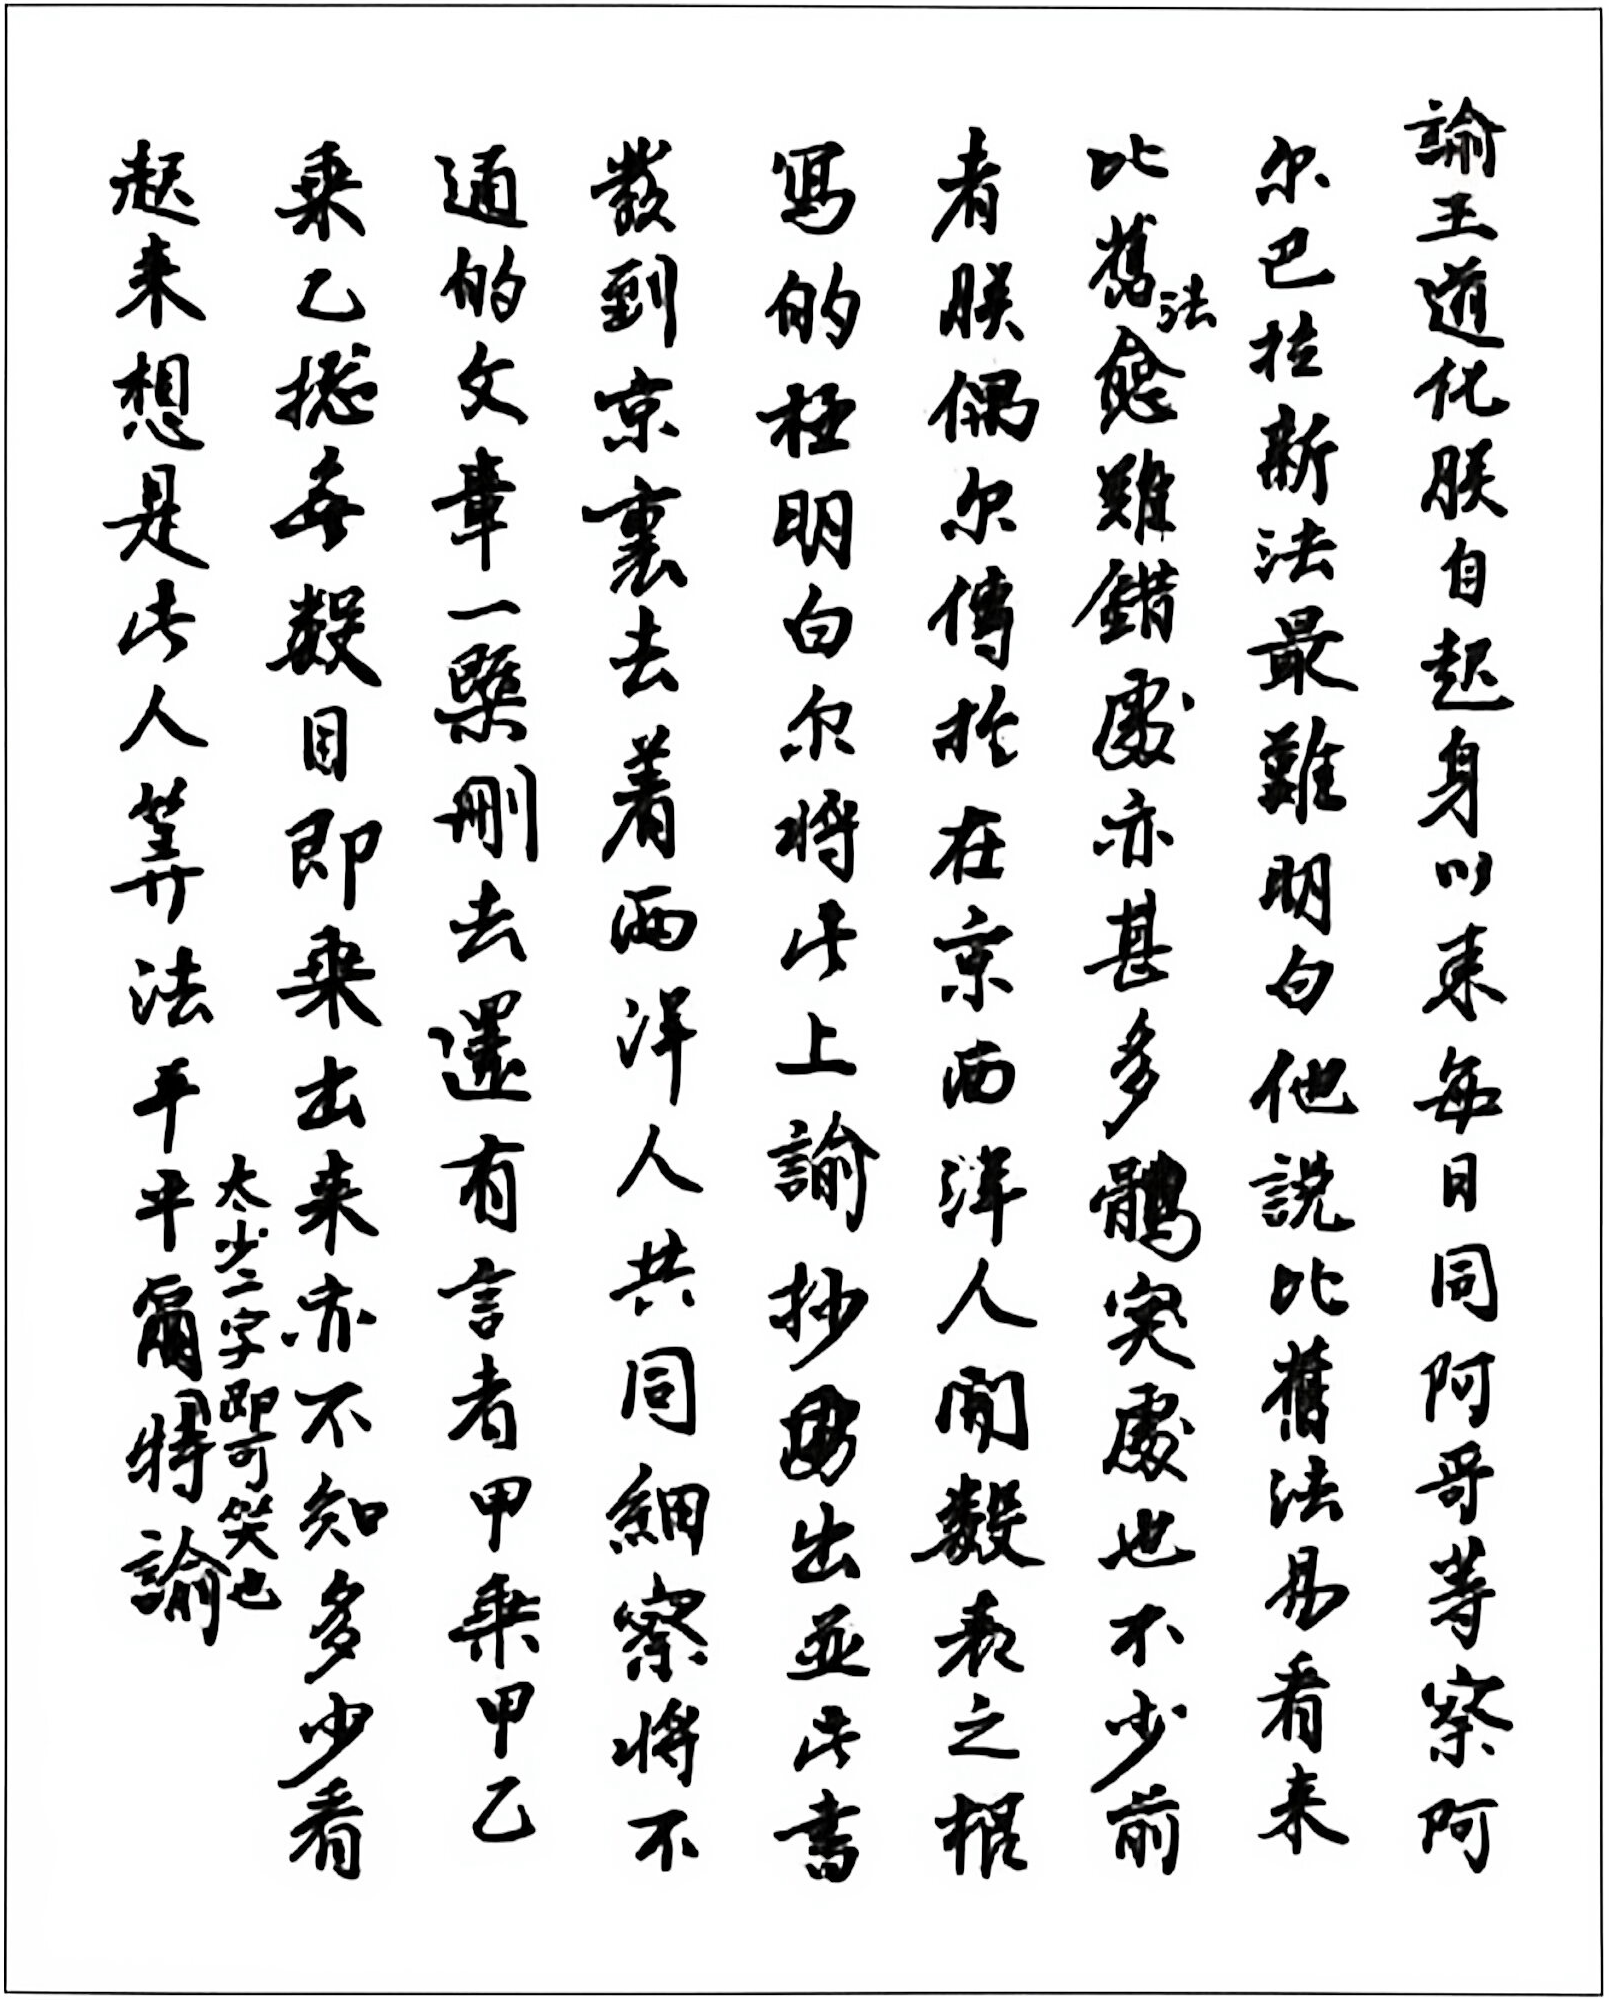
\includegraphics[width=\linewidth,height=.57\textheight,keepaspectratio]{assets/figures/kangxi-algebra-edict.png}
\caption*{图8.1\quad 康熙谈论代数谕旨}
\BookFloatNotes{图片来源：《清中前期西洋天主教在华活动档案史料》，1:52。}
\BookFloatNotes{谕王道化：朕自起身以来，每日同阿哥等察阿尔巴拉新法，最难明白。他说比旧法易，看来比旧法愈难，错处亦甚多，鹘突处也不少。前者朕偶尔传于在京西洋人开数表之根，写的极明白。尔将此上谕抄出并此书发到京里去，着西洋人共同细察，将不通的文章一概删去。还有言者：甲乘甲、乙乘乙总无数目，即乘出来亦不知多少。看起来想是此人算法平平尔，太少二字即可笑也。特谕。}
\end{figure}%
\par
% 原书页码：296；段落
现当代史家引用到这份谕旨都集中在康熙的最后两句，评点代数%
“算法平平”“可笑”上。这几个词就是吸睛的冲突部分，用来说明康%
熙自大无知，耽误了西学、科学引人中国。\NoteRef{epilogue}{3}除了把这几个冲突字眼%
拣出来，没有人关注这段话的前半部分，也没有人想要理解为什么康%
熙说“算法平平”“可笑”。%
\par
% 原书页码：296；段落
第一句：“朕自起身以来，每日同阿哥等察阿尔巴拉新法。”“阿尔%
巴拉”就是代数，是Algebra的音译。康熙皇帝外出，一路上还和他%
的皇子一起研读代数这个当时全新的数学科目。这说明什么？如果在%
旅途的火车上，我们看到一个人拿着一本代数书看，我们的反应是什%
么？康熙整篇谕旨，说的是他试着在理解这本代数书，但明显没有看%
懂，最后指示他的奴才把这本书拿去让西洋人共同“细察”，把问题%
写明白。%
\par
% 原书页码：296–297；段落（跨页续段）
代数现在看起来是数学中的基础内容，但对当时的欧洲传教士来%
说也是一门新学科。代数并不是希腊罗马时期发展出的传统数学部分，%
而是阿拉伯人花拉子密（Al-Kwarizmi）9世纪（相当于中国唐朝时期）%
创立的。代数在欧洲各种语言中都叫Algebra，这个词是阿拉伯文的音%
译。12世纪意大利人把花拉子密的著作翻译成了拉丁文。16世纪法国%
数学家韦达（Francois Viète，1540—1603）发展出了用字母来演算的新%
代数，这也是我们现代人所学代数的基础。从康熙朝编订的《数理精%
蕴》可以看到，大量有代数思维的演算已经被康熙重视和接受了。《数%
理精蕴》是康熙和皇三子实际参与编订的书。里面有许多二元二次方%
程的题，还有一元三次方程需要求立方根的题以及求解。康熙和他的%
儿子没有弄明白的是代数和方程使用的意义是什么。当时康熙对不出%
现数字，以及为什么要这样来演算数学并不理解，也就是康熙谕旨中%
抱怨的“无数目，即乘出来亦不知多少”。%
\par
% 原书页码：297；段落
代数其实是人类数学思维的一次重大革命。数学本来是一种确定%
性的表达，而代数是在确定性中融入了不确定性，也就是用字母表达%
的部分。欧洲从韦达开始，到经过笛卡尔完善的新代数，也是经过了%
上百年才慢慢被消化，一直到牛顿把代数应用到物理中，代数这个数%
学工具才逐渐开始显示其大用处。牛顿在物理领域取得突破前，是剑%
桥大学教代数的教授。他之前的物理大师，如伽利略和开普勒等都还%
没有使用代数。1707年牛顿的《广义算术》（\textit{Arithmetica Universalis}）问%
世，这是牛顿在剑桥关于代数和方程方面的讲稿汇编。在这本书中，%
牛顿把开普勒的天体轨道运算重新用代数的方法来演算，展示出了代%
数演算的优势。牛顿还用一道道题，具体讲解代数的用处。比如，一%
个石头从井口落下，知道从石头开始下落到听到底部传来回声的时间，%
问井有多深。这道题中，牛顿把深度设为\(x\)，这样石头落下和回声传%
回来的两段物理过程中的距离都是\(x\)。方程建立在时间\(t=t_1+t_2\)上（\(t_1\)%
是石头落下的时间，\(t_2\)是回声传回的时间，两段都用距离\(x\)和石头以%
及声波运行速度来求得）。这样两段物理过程就通过未知的距离\(x\)联系%
到了一起。\NoteRef{epilogue}{4}%
\par
% 原书页码：297–298；段落（跨页续段）
牛顿的《广义算术》严格来说并没有多少学术上的突破，但其主%
要特点是实用，讲的是技巧，从而大大推动了代数的使用范围。牛顿%
当时对代数在应用上的推动，有点类似于微软做出了Windows系统，%
大大拓展了电脑的使用范围。当时给康熙讲代数的是法国傅圣泽神父，%
他1699年就到中国，大概率他没有看过牛顿的大作，对代数真正的%
用途也所知有限。为了方便康熙阅读，傅圣泽没有用字母来替代未知%
量，而用的是天干地支。\NoteRef{epilogue}{5}比如他给康熙的书中讲的甲与乙之和的平方%
等于甲平方加乙平方再加二倍甲乙相乘的乘积。这是大家都熟知二元%
二次方程中的公式\((x+y)^2=x^2+2xy+y^2\)。康熙能看懂这个，但是他不%
知道这样做的用处是什么。所以他会评价“他说比旧法易，看来比旧%
法愈难”。上面提到石头下落的题里，牛顿就讲到了一元二次方程几%
个公式的应用。由于石头落下还涉及自由落体下坠，也就是下落距离%
和时间平方成正比（\(d=kt^2\)），因此在这道例题中，牛顿就展示了求解%
技巧，用到一元二次方程中的求根公式：%
\[\displaystyle x=\frac{-b\pm\sqrt{b^2-4ac}}{2a}\]
\par
% 原书页码：298；段落
这个求根公式就是从\(ax^2+bx+c=0\)这个一元二次方程的标准式中推出来%
的。代数对当时的传教士来说，也是新东西，没有办法给康熙深入讲%
解分析也情有可原。在不明白代数用途的情况下，康熙读完代数后的%
第一反应其实和当时欧洲人的反应是一样的，对为什么学习代数以及%
代数的用处有疑问，对思维转变有不适应。%
\par
% 原书页码：298；段落
平心而论，就算不知道代数在欧洲的发展历史，如果不是先入为%
主对论证某些理论有需求，任何看到康熙读代数这段史料的人，都会%
感叹康熙学习数学之用功。而且康熙为什么要写这封谕旨？这封谕旨%
的接收人王道化，是康熙在宫里的奴才。他写这封谕旨传回京城的目%
的不是要嘲笑代数新法“可笑”，而是要让奴才把它拿给传教士重新%
书写编辑。%
\par
% 原书页码：299；段落
康熙的奴才确实把这封谕旨抄了一份，交给传教士，让他们赶紧%
重新把代数整理翻译清楚。这份谕旨的抄件在罗马还有保留。尽管康%
熙文字中说新法“可笑”，但他直觉到其中有新东西，所以一直在催%
促传教士把代数重新写清楚。其实传教士当时要介绍代数，也是不容%
易的。这要求他们自已对代数要有透彻的理解，知道这个方法的新意%
到底在哪里。现在回看历史，所有人都同意代数是无可取代的数学工%
具。但这个认识是因为后来的发展让代数的作用完全显露了出来。笛%
卡尔（1596—1650）创造了坐标系，用代数来计算几何，又经过牛%
顿和后来的数学家欧拉的完善，代数被用来对世间万物进行运算经过%
了上百年的发展历程。后来所有科目的科学运算，都离不开代数和方%
程，这是我们都知道的事。但当时的传教士并不能完全看到代数未来%
的妙用。除了代数知识以外，要把问题给康熙讲清楚，还要求中文水%
平高。注意这里要求的中文水平是写作水平，这是中文学习中最难的%
部分。当时在京的传教士懂代数的有三人，但只有傅圣泽一人勉强能%
写中文。1716年（康熙驾崩前六年），有号称懂数学的新传教士来华%
时；康熙还让皇三子专门去询问欧洲有没有新的求立方根和平方根的%
方法。\NoteRef{epilogue}{6}康熙其实要问的就是代数中的求根方法。中国传统数学中有%
平方根和立方根的求解方法，康熙也是知道的。他想要知道的是代数%
里面的新方法。%
\par
% 原书页码：299–300；段落（跨页续段）
比如康熙朝编订的《数理精蕴》中有应用题，列出的算式是\(x^3+8x=1824\)%
（书中没有用\(x\)，但用代数写出来就是这个等式），这就需要%
求立方根。\NoteRef{epilogue}{7}康熙想知道的立方根求解方法，也是困扰了欧洲上百年%
的问题。按照代数的方法，立方根求解中会出现负数开根号的情况。%
最后解决这个问题是定义出了虚数概念。虚数在英文中叫Imaginary%
\space%
number，直接翻译过来就是“想象出来的数字”。虚数最早是由笛卡%
尔提出，但在与实数一起进行运算时还有大量实际操作问题。而虚数%
相关的各种问题完全解决是在18世纪中期，也就是在中国的乾隆年%
间。康熙想要知道的问题可能现在看起来不难，但放在当时都是大问%
题。康熙在得不到好的代数书翻译的情况下，让传教士直接把他们能%
找到的所有西文代数书都交给皇三子。\NoteRef{epilogue}{8}六十多岁的康熙还寄希望自%
己能和他的皇子一起把代数弄明白。在数学中，“元”“次”和“根”%
等专门术语都是康熙翻译的。%
\par
% 原书页码：300；段落
除了在历史细节上经不起推敲，基于清初传教士来华而衍生出%
的各种文化冲突理论还有一个先天缺陷：就是无法解释传教士事业在%
康熙时代的辉煌。如果中国传统文化和西方文化真的不能调和，西%
方科学和中国传统思维有冲突，那么为什么传教士在康熙年间能成%
功，教徒人数成几何级倍数增长，西方知识大量涌入？康熙一朝就%
是六十一年。六十一年放在历史长河中很短暂，但这也是传教士在%
中国，和中国百姓一天天、一年年过出来的六十一年。不能因为后%
来雍正禁了教，就选择性忽视之前调和的日子。传教士在康熙朝得%
到了各种优待不假，但百姓人教都是他们自己的选择。寺庙、道观，%
教堂，老百姓选择去哪里，到底有没有不可调和的文化冲突，他们%
是在用行动给出答案。%
\par
% 原书页码：300–301；段落（跨页续段）
这又涉及一个历史的评判问题。历史应该最少有两次评判。一是%
当时的人——历史参与者流露出的主观感觉，这可以算作一种评判。%
二是后来人综合历史上下文的评判。这两种评判可以不同，但是后来%
的历史评判不能无视当时人自身的感受。比如藏传佛教中一路几千公%
里磕长头的苦行。如果一位苦行的信徒成为了历史人物，变成了历史%
研究对象，这时候他磕长头朝拜和朝拜时的满足与期待才是历史中的%
存在。后来人的历史评判，需要在当时人的行为和感受基础上来做评%
判。如果完全不考虑当时人的主观感受，而站在现代科学的立场，认%
为他的苦行没有价值和意义，那就跟当时历史没有了关系，这种评判%
严格讲也不属于历史研究。本书第二章讲到杨光先时，其实已经谈到%
过这个问题。杨光先的书和言论在当时没有得到士人的认同，没有引%
起反响。因而无论他去世一百年后有多少人关注他的观点，历史的事%
实只有一个，就是他的书当时没有引起反响和认同。所有明末清初相%
关的历史论述，也都应该建立在杨光先在当时没有得到主流文人认可%
这个历史事实的基础上。而鸦片战争以后，杨光先的论说在特定的历%
史条件下被重视，被研究，这属于另外一段历史，和明末清初的历史%
应该区分开来。两段历史的不同，西方已经形成了一个专门的研究派%
别，就是后世“接受理论”（reception theory）。比如杜甫，唐朝以后各%
个时代对他的作品有不同的评论和看法，但这些评论和看法不能当成%
杜甫自身历史的一部分。\NoteRef{epilogue}{9}%
\par
% 原书页码：301–303；段落（跨页续段）
明末清初传教士一批一批来到中国，他们就是当事人。在我们做%
出任何关于当时中西文化对比的判断时，应该首先看他们怎么说。传%
教士来到中国后，确实观察到了中西文化方方面面的差异，而且还留%
下了各种记录。但他们认为那些文化差异是冲突，而且是不可逾越的%
吗？显然不是。全球化之初，商人和传教士是最早走遍世界的两大群%
体。跟牟利的过往商人不同，传教士到了世界各地都需要深度融入当%
地社会。因此，他们的记录都是他们在当地生活后的切身体验。当时%
生活在中国的传教士，在定居中国前，都到过许多国家，也了解世界%
各个地区的文化差异。对他们来说，中国社会和文化是很包容的，是%
在传统文明发达的地区中很有可能接受基督教的地方。当他们在中国%
发现已在开封定居几百年的犹太人，并得知他们依然保持着自己的信%
仰时，就感叹过传统中国的包容。当时耶稣会神父还去到印度的莫卧%
儿帝国（1526—1857）。他们也走入了当时莫卧儿帝国一代明君阿克%
巴大帝（Akbar the Great，1542—1605）的皇宫。但是面对伊斯兰势%
力，耶稣会神父能够发挥的空间很小。\NoteRef{epilogue}{10}同时，意大利的耶稣会神父%
伊波里托·德基德利（Ippolito Desideri，1684—1733）在 1716 去到了%
中国西藏。当时西藏知道一些耶稣会神父在北京的事迹，因而伊波里%
托在西藏还受到了款待，被允许留在拉萨学习藏语、佛教和西藏文化。%
西藏并没有排斥这位意大利去的神父，还允许他建立一个小的天主堂%
（一个小房间）。只是伊波里托神父自已发现很难把基督教传进西藏，%
很难找到信徒。\NoteRef{epilogue}{11}如果按今天流行的经济学观点，我们把信仰需求看%
作一个市场的话，那么可以说基督教作为一款信仰产品进人不了西藏%
市场，因为那里的本土信仰产品已经足够强大。\NoteRef{epilogue}{12}但当时的内地不一样，%
基督教作为信仰产品是能够进入到内地的，内地的百姓和主流文人都%
抱有一种开放的观念，把基督教当作一个外来的新产品在看待。尽管%
来华的传教士在对待中国传统习俗的态度上有分歧，但那是他们内部%
的分歧。他们在中国文化和中国土地能容纳西方科学和宗教这个大问%
题上是没有分歧的，所以我们看到，不同的修会都在增派人手到中国。%
传教士内部的分歧，就像今天跨国大公司不同部门之间对产品如何进%
入中国市场，如何对待中国传统消费习惯，以及如何让产品本土化的%
过程中有分歧是一样的。佛教于汉代进人中国以后，如何让佛教本土%
化，如何接入中国传统观念和文化，也是一个持续了上千年的问题。%
\par
% 原书页码：303；段落
对于当时的传教士和教皇来说，中西文化没有冲突，冲突的只是%
他们天主教内部的不同派别。罗马教皇收到康熙的红票，给康熙的回%
信中说：“我们从来没有想到过，我们对教内做出的规定会让您不高%
兴。”天主教即便是在欧洲内部争论时，对孔子以及儒家传统都抱有十%
足的敬意，认为孔子提倡的“慎终追远”、重视丧葬、敬畏神灵是和%
天主教教义精神暗合的。他们并没有想过要反对这个传统，而他们要%
规定的只是受洗的教徒，要他们坚持心中只有一个神灵，就是天主，%
入教之后不能再求祖先等其他神灵保佑和庇护了。在这个思路指导下，%
他们规定了教徒哪些传统活动能参加，哪些不能。在传教士和教皇眼%
中，中西文化在某些具体操作上是有差异的，但不是互相冲突，是可%
以共存的。后来的历史其实也证明了传教士的基本判断。当儒家文化%
圈里的中日韩决定引进西方文化的时候，都很快速从容地做到了。在%
引进西方文化的历史进程中，这几个国家真正担忧的是西方文化是否%
引进得太多、太快。%
\par
% 原书页码：303–304；段落（跨页续段）
哪怕在雍正禁教以后，也没有任何传教士认为这是中西文化冲突%
所致。一切不过是宫廷政治罢了。雍正禁教在当时传教士看来也只是%
暂时的挫折。康熙初年鳌拜时期，在汤若望被参劾后，传教士的教堂%
都被没收了，后来又靠南怀仁东山再起。雍正时期北京的传教士就在%
等待下一次东山再起的时机。1735年，雍正去世，乾隆登位，康熙朝%
就活跃于北京官场的巴多明神父马上认为这是一次机会。他找到了内%
阁官员和康熙的皇十二子，让他们帮忙活动，同时他自己也写了一份%
折子。尽管最后巴多明没能说动乾隆，但这份折子充分说明了传教士%
的希望和等待。%
\par
% 原书页码：304–305；段落（跨页续段）
乾隆登基后，尽管他没有像康熙那样允许天主教传播，但和雍正%
不一样，乾隆是愿意使用传教士的。圆明园的喷水池部分就是传教士%
设计，仿照欧洲宫廷建造的。近年来颇有名气的十二生肖兽首，就是%
安装在圆明园里用作喷水龙头之用的。巴多明神父年迈之时，还曾上%
奏乾隆，说自已年纪大了，希望能允许两个年轻传教士来北京照顾他。%
乾隆允准了。来的两个传教士就是来继承他北京的教堂的。巴多明于%
1741年在北京病逝，是经历了康雍乾三朝的元老。像巴多明一样在北%
京等待机会的传教士还有很多。鼎鼎大名的郎世宁也是这样。康熙朝%
就到北京的他，一直在宫廷里作画，乾隆的母亲就很赏识他，还坚持%
要乾隆给郎世宁安排个官职，发薪俸给他。\NoteRef{epilogue}{13}郎世宁从雍正1724年禁%
教，一直到他1766年去世，又在北京待了四十多年。他到死都还在%
等待机会，希望有一天能让天主教被朝廷重新认可。乾隆登基后不久，%
在澳门的传教士专门开过会讨论天主教在中国是否还有希望。会上没%
有人认为他们的困难来自于中西文化差异或者是文化冲突，他们都认%
为问题的关键是皇帝的想法。他们都寄希望于北京的传教士能像南怀%
仁当年一样，找到机会。乾隆中期以后，以郎世宁为代表的宫廷传教%
士，通过他们的努力，确实也让乾隆对传教士的看法有所改变。乾隆%
不仅越来越多地使用传教士，还像康熙一样把传教士召人了他的内务%
府。一些文件显示，传教士又开始找内务府，而不是朝廷部门来处理%
他们在北京生活上的具体问题。\NoteRef{epilogue}{14}现存的奏折中可以看到，1760年代后，%
乾隆又像康熙一样，命令两广总督选送有技术的西洋人到北京。而且%
1778年以后，乾隆还几次问询沿海官员为什么没有有技术的西洋人前%
来。乾隆的这些谕旨，最直接地说明传教士耐心等待时机的既定思路%
是没有错的。%
\par
% 原书页码：305；段落
早年制定政策的传教士没有想到的是，欧洲教廷内部发生了巨变。%
从1750年代开始，耶稣会在欧洲受到排挤打压，各国相继取消了耶%
稣会。1773年教皇宣布解散了耶稣会。（直到1956年，罗马教廷才又%
恢复了耶稣会的地位。现任教皇方济各就是耶稣会神父。）所以1760%
年代以后，留守在北京的耶稣会神父基本没有了欧洲的支持。在乾隆%
日渐对西方感兴趣的时候，耶稣会没有能力再派人到中国来。乾隆发%
现来北京效力的西洋人越来越少，其实也是这个原因。%
\par
% 原书页码：305–306；段落（跨页续段）
当然历史就是历史，结果就是传教士没有等来基督教解禁的那一%
天。但有这样的结果，不等于必然是这样的结果。长期以来，写史的%
人都希望妙笔生花，把一个个故事讲得逻辑井然，头头是道，同时还%
希望自已能发前人之未发，概括出事件背后的大势。在历史中总结规%
律的想法源自于18—19世纪的西方史家和哲学家，他们受到西方科%
学革命的影响，希望像研究自然界的物理现象一样，找到历史发展的%
规律。寻找历史规律主导了现当代历史研究，同时也支配了现当代的%
历史书写。这一影响最具体的表现就是史家热衷于讲抽象的“大”历%
史，而忽视了历史中的个人和那些有血有肉的细节，以及个体生命轨%
迹中展现出的偶然性和不确定性。就是华语世界的一流史家如陈寅恪，%
他那部拒绝历史规律、深挖历史细节的《柳如是别传》，在出版半个%
世纪后，依然不被重视，甚至有评论为陈寅恪惋惜，认为这部书浪费%
了他晚年的时间和心血。但如果我们能够接受历史并不抽象，它就是%
由一个一个鲜活的个体共同演绎出来的，那么我们就应该重视历史中%
的个人，以及接受个人命运及其带有的偶然性和不可测部分都可能会%
影响到历史。%
\par
% 原书页码：306；段落
比如前面提到的带了7000本欧洲书籍在明朝万历年间再次进入%
中国的金尼阁神父。回到中国后，他渐渐开始后悔在教皇面前赞同利%
玛窦把天主教的神（deus，英文译为god）翻译成中文“上帝”这个词。%
随着他对中文研究的深人，他认为这个基督教里最关键的词翻译得不%
对，铸成了不可挽回的错误。最后他在1628年一天的清晨四点和神父%
们一起做完祷告回到房间后，上吊自杀了。自杀在天主教神父中是极%
其罕见的，而且对于教会来说是丑闻。当时的罗马教会内部都是用密%
信外加密码交流此事。\NoteRef{epilogue}{15}之前金尼阁神父为买书到中国一事，在欧洲%
云游募捐筹款，这让他在欧洲很有名气。现在纽约大都会博物馆还藏%
有一副鲁本斯（Peter Paul Rubens）在金尼阁到安特卫普（Antwerp，比%
利时城市）募捐时，为金尼阁画的身穿中国儒家冠服的全身像（见图%
8.2）。金尼阁神父出人意料地自杀身亡，对中国来说，最大的损失就%
是他要进行的西学翻译事业戛然而止了。我们其实谁也不知道，玄奘%
要是在路上遇到强盗，没能把佛经带回长安，没把印度的佛经翻译出%
来会怎样影响佛教在中国的传播。不过二人个体生命中的偶然性，肯%
定或多或少都影响了某段历史的演进。%
\par
% 原书页码：306–307；段落（跨页续段）
历史在一个个的个人选择中充满着不可预料的偶然，正如我们现%
在的世界在个人决策下充满着不可预测的偶然一样。现在的世事就是%
未来的历史，而历史就是以前的世事。就像2019年开始的新冠疫情，%
% 原书页码：307；图表（图题／表题所在页）
\begin{figure}[tbp]\phantomsection\label{fig-323-0}
\centering
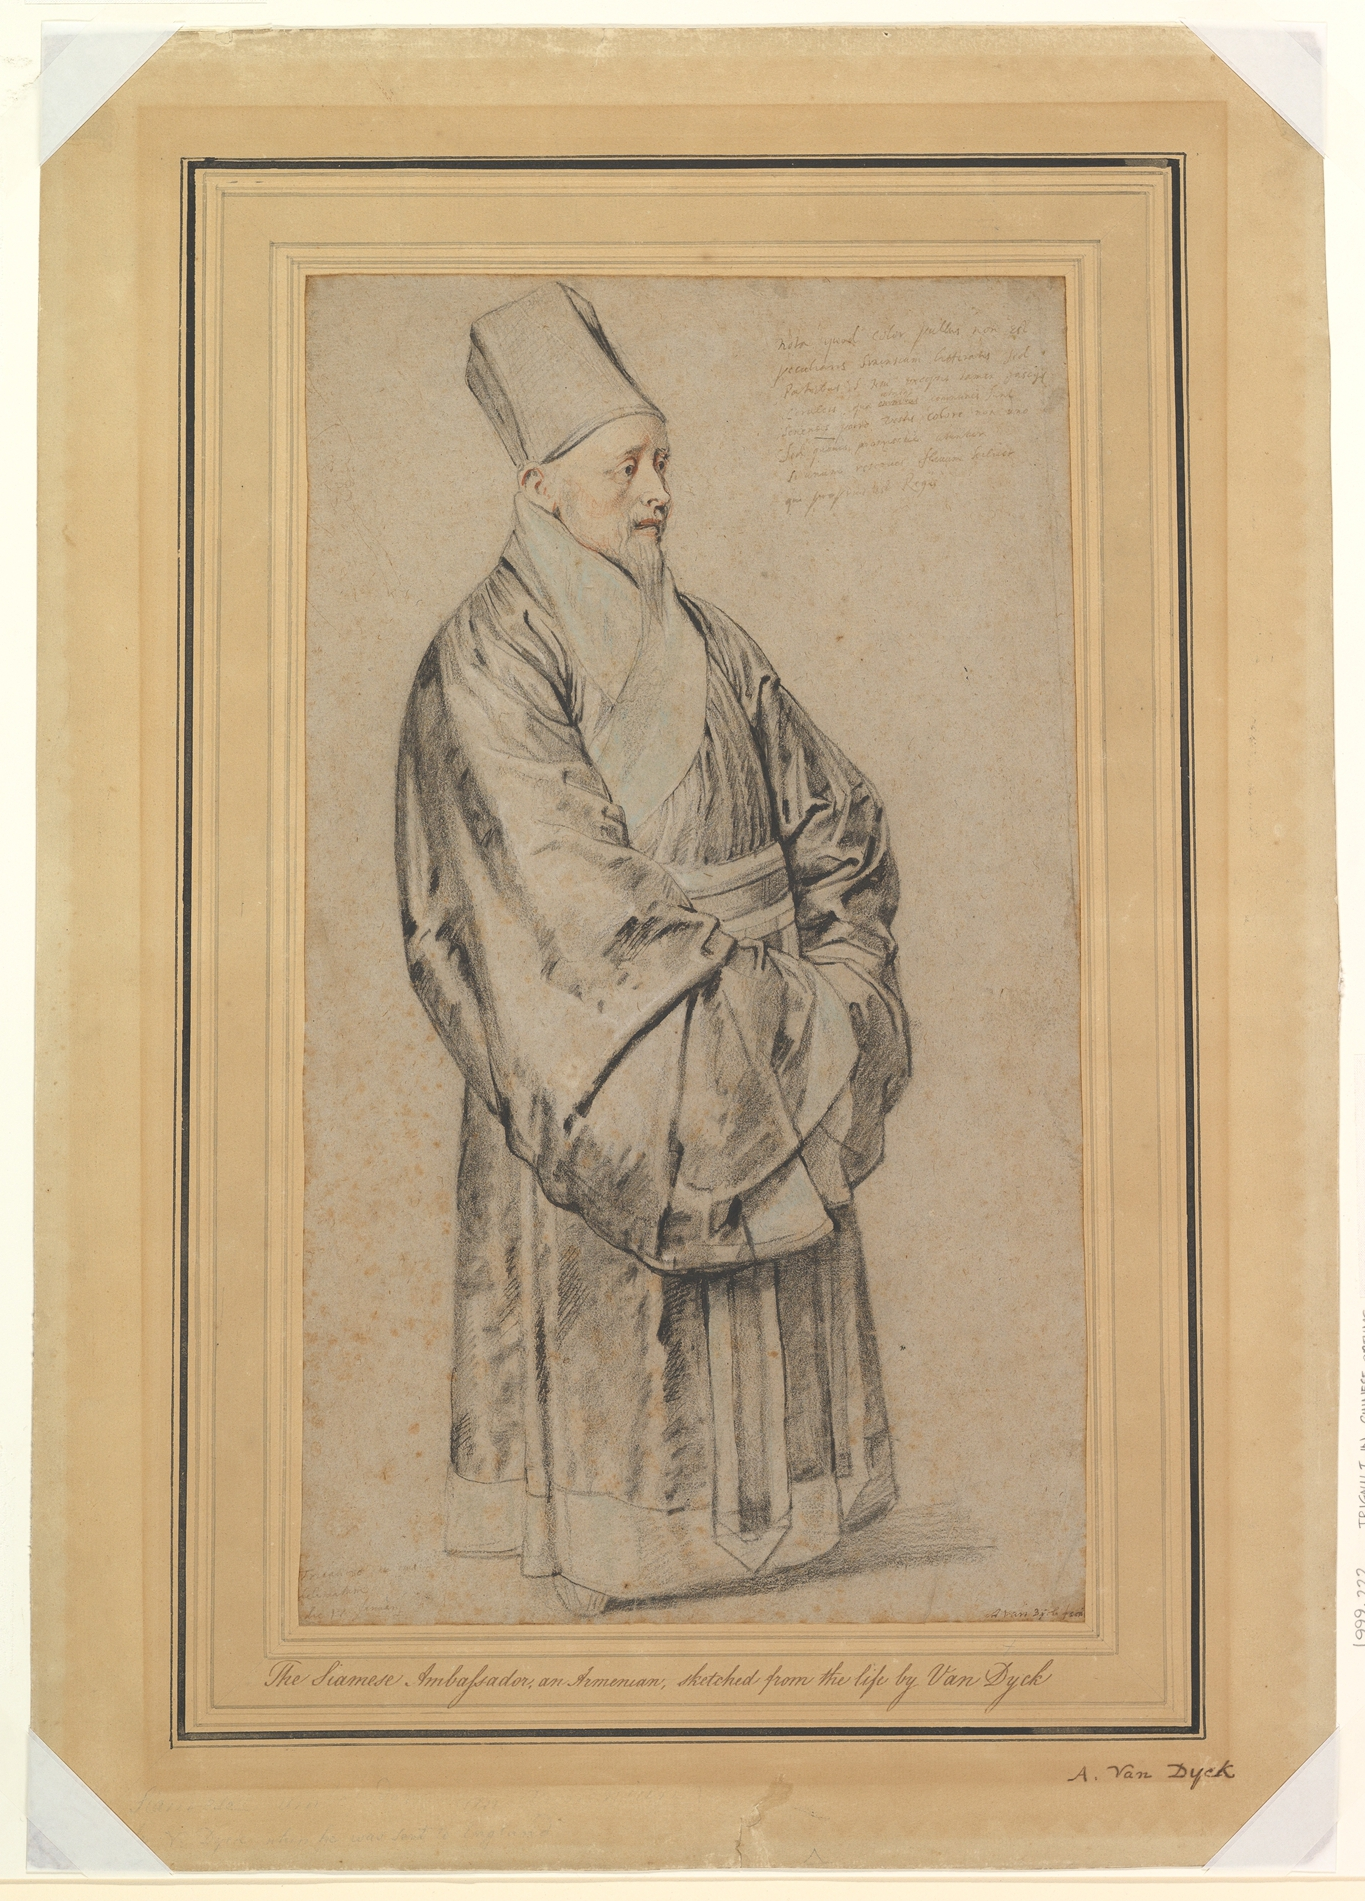
\includegraphics[width=\linewidth,height=.76\textheight,keepaspectratio]{assets/figures/trigault-portrait.jpg}
\caption*{图8.2\quad 鲁本斯绘金尼阁着儒服全身像}
\BookFloatNotes{图片来源：纽约大都会博物馆网站。文件编号337844。}
\end{figure}%
对于个人、国家、世界都是一个偶然性事件，到底它会怎样影响到历%
史的演进，我们不知道，但我们能感受到的是，这个突然出现的事件，%
会是无数个人生命中的变量。%
\par
% 原书页码：307–308；段落（跨页续段）
在本书涉及的历史时段中，康熙对西学的兴趣和雍正对佛教的%
修行也都是横跨古今、独一无二的个案。恰好传教士和西学相关的%
历史都和这两个皇帝的个人喜好紧密相连。1722年秋，康熙已经出%
去打过一次猎了，回到北京后六十八岁的他竟还意犹未尽。当他再%
次离开北京去打猎的时候，身体状态应该是不错的。可惜出去不久，%
他就感染风寒，很快去世了。康熙在病床上匆匆开始了传位，皇四%
子也在完全没有预兆的情况下，突然登基了。几个月后，皇三子被%
发配去给康熙守陵墓，他负责的西学事业也随之停止。又过了几个%
月，传教士的教也被禁了，这在影响天主教人华的同时也影响了西%
方科学的传播。当时所有的西方知识都是靠这些来华的传教士亲自%
带到中国的。他们人不再来，西学传播的渠道也随之减少。对于中%
国来说，这就使得中国错过了西方科学革命中最重要的18世纪。在%
谈论近代西方科学革命时，很多人都喜欢上追希腊罗马。但实际上%
希腊罗马后一千多年，欧洲科学并没有什么大发展。欧洲科学革命%
中最关键的反而是从阿拉伯传到欧洲的代数，以及在代数上发展出%
的微积分这两个实用的数学工具。牛顿就是使用这两个工具来解释%
现实世界的第一人，开启了18世纪欧洲科学的井喷式发展。可惜在%
代数就快要进人中国时，持续了大约一百年的西学东传，随着康熙%
的驾崩和雍正的登台而逐渐停止了。当然历史无法假设，要是康熙%
之后的雍正皇帝没有为难皇三子，是不是西学引进还能持续，从而%
改变中国的历史进程？我们无从知道答案。但可以知道的是，西学%
没能继续传播并不是中国传统文化的问题，也不是传统士人不接受%
西学的问题。毕竟从万历年间算起，中西互通在明清之际切切实实%
地走过了一百年。%
\par
% 原书页码：309；段落
传统中讲“一朝天子一朝臣”，康雍之间的皇位更替不仅改变了%
传教士和康熙众多皇子的个人命运，同时也改变了那些跟这些人命%
运紧密相连的历史。庙堂之上的变动，我们后来者似乎能带着“后%
见之明”来评点一番；但变动发生前，谁也预料不到，哪有什么规%
律可总结？史家要做的，也许就是把发生过的故事和细节挖掘出来%
就好。%

\clearpage\markboth{注释}{注释}
\BookUnnumbered{注释}
\begingroup\small\setstretch{1.15}
\NoteChapter{第一章\quad 佟家的奴才}
% 原书页码：311；注释 1:1
\NoteEntry{1}{1}{%
该奏本藏于台湾史语所内阁大库档案，档案编号为038202。内阁大库档案网站有该奏本%
的图像供调阅。%
}
% 原书页码：311；注释 1:2
\NoteEntry{1}{2}{%
关于两位神父在张献忠大西朝的史事，参看：Zürcher, “In the Yellow Tiger's Dcn: Buglio and%
\space%
Magalhāes at the Court of Zhang Xianzhong, 1644-1647", 355-374.%
}
% 原书页码：311；注释 1:3
\NoteEntry{1}{3}{%
关于二位神父到京后的史事，参看：Dunne, Generation of Giants, 327；魏特，《汤若望传》，%
396,401。%
}
% 原书页码：311；注释 1:4
\NoteEntry{1}{4}{%
参看安文思的记录： Magalháes, A New History of China, Containing a Description of the Most%
\space%
Considerable Particulars of That Vast Empire, 346.%
}
% 原书页码：311；注释 1:5
\NoteEntry{1}{5}{%
Oxnam, Ruling from Horseback, 47-49.%
}
% 原书页码：311；注释 1:6
\NoteEntry{1}{6}{%
本文关于两位神父从四川到北京的经历，主要来自两方面材料。一是利类思神父在安文%
思神父1677年去世以后，为他写的一篇简短的传记。在传记开头，利类思自称是“与%
安文思36年未曾分离的挚友，传记于1677年从北京寄出”。后来这篇传记附在安文思%
神父写的《新中国史》书后，于1688年在伦敦出版。第二个材料是，古洛东注解的《圣%
教入川记》。古洛东是法国传教士，原名 Francois Marie Joseph Gourdon。他 19 世纪末年%
人华后在重庆传教，后来在上海从一位耶稣会士那里得到一部手写本，内容是关于利类%
思、安文思明末在成都开辟四川教区的往事。由于古洛东也在四川传教，所以他为这部%
手写本中记录的人物、地点作了注解，最后在1918年出版了该书。该书记录了许多利%
类思、安文思在张献忠朝廷的所见所闻，以及后来他们跟随豪格大军去北京的历史细节。%
Buglio, “An Abridgement of the Life and Death of F. Gabriel Magaillans”, 340-352;古洛东,《圣%
教入川记》。对于两位神父的传教经历，参看：汤开建，《沉与浮：明清鼎革变局中的欧%
洲传教士利类思与安文思》。%
}
% 原书页码：311；注释 1:7
\NoteEntry{1}{7}{%
Buglio, "An Abridgement of the Life and Death of F. Gabriel Magaillans", 345.%
}
% 原书页码：311；注释 1:8
\NoteEntry{1}{8}{%
Buglio, "An Abridgement of the Life and Death of F. Gabriel Magaillans", 346.%
}
% 原书页码：311；注释 1:9
\NoteEntry{1}{9}{%
古洛东，《圣教人川记》，57。%
}
% 原书页码：311；注释 1:10
\NoteEntry{1}{10}{%
古洛东，《圣教人川记》，59。%
}
% 原书页码：311；注释 1:11
\NoteEntry{1}{11}{%
古洛东，《圣教人川记》，52。%
}
% 原书页码：312；注释 1:12
\NoteEntry{1}{12}{%
古洛东，《圣教人川记》，55-56。%
}
% 原书页码：312；注释 1:13
\NoteEntry{1}{13}{%
古洛东，《圣教人川记》，55;Buglio, “An Abridgement of the Life and Death of F. Gabriel%
\space%
Magaillans", 345-346。%
}
% 原书页码：312；注释 1:14
\NoteEntry{1}{14}{%
Crossley, A Translucent Mirror, 140.%
}
% 原书页码：312；注释 1:15
\NoteEntry{1}{15}{%
《满文老档》，165。%
}
% 原书页码：312；注释 1:16
\NoteEntry{1}{16}{%
胡祥雨，《“逃人法”人“顺治律”考——兼谈“逃人法”的应用》。%
}
% 原书页码：312；注释 1:17
\NoteEntry{1}{17}{%
魏特，《汤若望传》，397。%
}
% 原书页码：312；注释 1:18
\NoteEntry{1}{18}{%
Chu, Law and Society in Traditional China, 9, 128, and 280-283; Sommer, Sex, Law, and Society in%
\space%
Late Imperial China, 5-8.%
}
% 原书页码：312；注释 1:19
\NoteEntry{1}{19}{%
对二人转到佟图赖名下，法国学者Pih根据当时传教士寄回罗马的报告，已有详细考证。%
参看： Pih, Le père Gabriel de Magalhães, 94-95.%
}
% 原书页码：312；注释 1:20
\NoteEntry{1}{20}{%
对此问题，20世纪以来，许多清史大家都有论述。认为佟家是汉化的满人的有：孟森，%
《清初三大疑案考实》，120-129；孟森，《明元清系通纪》1:190；陈寅恪，《柳如是别传》，%
1001-1002；牟润孙，《注史斋丛稿》，431-434。认为佟家是汉人，后来迁徙到东北的有：%
郑天挺，《清史探微》，22-28；Crossley，A Translucent Mirror,57-88。%
}
% 原书页码：312；注释 1:21
\NoteEntry{1}{21}{%
陈寅恪，《柳如是别传》，1001。%
}
% 原书页码：312；注释 1:22
\NoteEntry{1}{22}{%
《满文老档》，370；对于清初政治通婚研究，参看：Rawski,“Ch'ing Imperial Marriage and%
\space%
Problems of Rulership".%
}
% 原书页码：312；注释 1:23
\NoteEntry{1}{23}{%
相关内容佟世思在其撰写的家族史中有记载：佟世思，《先高曾祖三世行略》，408-409。%
}
% 原书页码：312；注释 1:24
\NoteEntry{1}{24}{%
Crossley, A Translucent Mirror, 62-63.%
}
% 原书页码：312；注释 1:25
\NoteEntry{1}{25}{%
《清史稿》，2:34。%
}
% 原书页码：312；注释 1:26
\NoteEntry{1}{26}{%
孟森在1936年的文章中就提到，包衣奴才就是身边最近的家奴。包衣奴才只是奴隶的%
一种。相关研究参看：祁美琴，崔灿，《包衣身份再辨》，117-128；孟森，《八旗制度考实》，%
260-262；郑天挺，《清代包衣制度与宦官》；左云鹏，《清代旗下奴仆的地位及其变化》；%
傅克东，《从内佐领和管领谈到清代辛者库人》；杜家骥，《八旗与清朝政治论稿》，435-%
488；鹿智钧，《根本与世仆：清朝旗人的法律地位》，185-194。在红学领域有关家庭内部%
运作的研究中，家中奴仆也是一个部分，这些红学研究对于了解清初奴仆也有贡献。比%
如杜家骥，《清代内务府旗人复杂的旗籍及其多种身份——兼谈曹雪芹家族的旗籍及其%
身份》。另外英文研究中，参看：Elliott,“Vocabulary Notes from the Manchu Archives 2: On%
\space%
the booi"", 18-21; Spence, T’ao Yin; Torbert, The Ch'ing Imperial Household Department; Crossley,%
\space%
A Translucent Mirror, 140-142; Elliott, The Manchu Way, 81–83.%
}
% 原书页码：312；注释 1:27
\NoteEntry{1}{27}{%
魏特，《汤若望传》，468。%
}
% 原书页码：312；注释 1:28
\NoteEntry{1}{28}{%
明代对使用红衣大炮获胜的报告，参看：《明熹宗实录》，68:1a。%
}
% 原书页码：312；注释 1:29
\NoteEntry{1}{29}{%
《明熹宗实录》，70:17b。%
}
% 原书页码：312；注释 1:30
\NoteEntry{1}{30}{%
《明熹宗实录》，79:19b。%
}
% 原书页码：312；注释 1:31
\NoteEntry{1}{31}{%
《皇朝文献通考》，636:461-462。%
}
% 原书页码：312；注释 1:32
\NoteEntry{1}{32}{%
整个行程，参看：Cooper, Rodrigues the Interpreter, 341-342.%
}
% 原书页码：312；注释 1:33
\NoteEntry{1}{33}{%
Cooper, Rodrigues the Interpreter, 338.%
}
% 原书页码：312；注释 1:34
\NoteEntry{1}{34}{%
张小青，《明清之际西洋火炮的输人及其影响》，72。%
}
% 原书页码：313；注释 1:35
\NoteEntry{1}{35}{%
张小青，《明清之际西洋火炮的输入及其影响》，75-76。%
}
% 原书页码：313；注释 1:36
\NoteEntry{1}{36}{%
黄一农，《红夷大炮与皇太极创立的八旗汉军》，77-78。%
}
% 原书页码：313；注释 1:37
\NoteEntry{1}{37}{%
对大凌河之战，魏斐德《洪业：清朝开国史》一书中有精彩论述。%
}
% 原书页码：313；注释 1:38
\NoteEntry{1}{38}{%
《皇朝文献通考》，194:55。%
}
% 原书页码：313；注释 1:39
\NoteEntry{1}{39}{%
《天聪五年八旗值月档（一）》，自《历史档案》，2000（4），4。%
}
% 原书页码：313；注释 1:40
\NoteEntry{1}{40}{%
牟润孙，《注史斋丛稿》，435。%
}
% 原书页码：313；注释 1:41
\NoteEntry{1}{41}{%
对于清朝突然能造出大炮，黄一农认为是满人在1629年突袭中，抓了一批汉人工匠。%
后来清朝铸造的大炮炮身上都刻有这些工匠的名字。同时，黄一农还注意到满人这段时%
间在大海打捞出的沉船中有一尊红衣大炮。于是黄一农认为这批汉人工匠通过模仿海中%
打捞出的大炮，成功仿制出了红衣大炮。我认为黄一农此论对冶炼技术中的技术难点估%
计不足。明末1620年代起，明朝的工匠就在积极仿制，希望制造出红衣大炮来。但是%
炮管等冶炼温度火候掌握不好，造出来的大炮有使用问题及安全隐患。因而明朝在1630%
年代都没有造大炮的技术，需要到澳门购买。所以说，清朝靠自己的能力解决了制造大%
炮中的各种技术问题，这种可能性是很小的。参看：黄一农，《红夷大炮与皇太极创立的%
八旗汉军》。%
}
% 原书页码：313；注释 1:42
\NoteEntry{1}{42}{%
黄一农，《天主教徒孙元化与明末传华的西洋火炮》，911-959。%
}
% 原书页码：313；注释 1:43
\NoteEntry{1}{43}{%
Cooper, Rodrigues the Interpreter, 350.%
}
% 原书页码：313；注释 1:44
\NoteEntry{1}{44}{%
董少新，黄一农，《崇祯年间招募葡兵新考》，78。%
}
% 原书页码：313；注释 1:45
\NoteEntry{1}{45}{%
董少新，黄一农，《崇祯年间招募葡兵新考》，79；黄一农，《红夷大炮与皇太极创立的%
八旗汉军》，90-91。%
}
% 原书页码：313；注释 1:46
\NoteEntry{1}{46}{%
孔有德被封“恭顺王”，参看：《满文老档》，1446。%
}
% 原书页码：313；注释 1:47
\NoteEntry{1}{47}{%
张小青，《明清之际西洋火炮的输入及其影响》，86。%
}
% 原书页码：313；注释 1:48
\NoteEntry{1}{48}{%
《清史稿》，234:9398-9399。%
}
% 原书页码：313；注释 1:49
\NoteEntry{1}{49}{%
关于清朝早期八旗中汉人以及他们成立汉军旗的起源，参看：Li,“The Manchu-Chinese%
\space%
Relationship", 1-32.%
}
% 原书页码：313；注释 1:50
\NoteEntry{1}{50}{%
陈寅恪，《柳如是别传》，158。%
}
% 原书页码：313；注释 1:51
\NoteEntry{1}{51}{%
《皇清开国方略》，341:205。%
}
% 原书页码：313；注释 1:52
\NoteEntry{1}{52}{%
关于地位的变化，参看：Li,“The Rise of the Early Manchu State”, 139-142.%
}
% 原书页码：313；注释 1:53
\NoteEntry{1}{53}{%
关于整个汉军八旗的形成，参看：Li,“The Manchu-Chinese Relationship”, 25.%
}
% 原书页码：313；注释 1:54
\NoteEntry{1}{54}{%
关于红衣大炮数量的估算，参看：黄一农，《红夷大炮与皇太极创立的八旗汉军》，92。%
}
% 原书页码：313；注释 1:55
\NoteEntry{1}{55}{%
《明清史料·乙编》，494。%
}
% 原书页码：313；注释 1:56
\NoteEntry{1}{56}{%
“乌珍超哈”就是汉军的意思。见：《钦定大清会典事例》，1111：1b。%
}
% 原书页码：313；注释 1:57
\NoteEntry{1}{57}{%
Ujen的满语本意，参看：Li,“The Manchu-Chinese Relationship”，25；又陈佳华、傅克东，《八%
旗汉军考略》，19。%
}
% 原书页码：313；注释 1:58
\NoteEntry{1}{58}{%
陈寅恪，《柳如是别传》，158。%
}
% 原书页码：313；注释 1:59
\NoteEntry{1}{59}{%
《大清太宗文皇帝实录》，卷9。%
}
% 原书页码：313；注释 1:60
\NoteEntry{1}{60}{%
《皇清开国方略》，341:262。%
}
% 原书页码：313；注释 1:61
\NoteEntry{1}{61}{%
《清史稿》，列传十八。%
}
% 原书页码：314；注释 1:62
\NoteEntry{1}{62}{%
Dunne, Generation of Giants, 216.%
}
% 原书页码：314；注释 1:63
\NoteEntry{1}{63}{%
Dunne, Generation of Giants, 217。%
}
% 原书页码：314；注释 1:64
\NoteEntry{1}{64}{%
Dunne, Generation of Giants, 318.%
}
% 原书页码：314；注释 1:65
\NoteEntry{1}{65}{%
《火攻挈要》，1643。%
}
% 原书页码：314；注释 1:66
\NoteEntry{1}{66}{%
萧若瑟，《天主教传行中国考》，247。有学者认为此人是尚可喜而非孔有德。%
}
% 原书页码：314；注释 1:67
\NoteEntry{1}{67}{%
孙元化没有听孔有德劝告跟他一起降清。不过，后来孔有德对孙元化一直心存挂念。当%
他得势以后，还主动照顾孙元化的后人。参看：黄一农，《天主教徒孙元化与明末传华的%
西洋火炮》，945。%
}
% 原书页码：314；注释 1:68
\NoteEntry{1}{68}{%
孔有德是孙元化部下，有跟西洋人打交道的经验，最后再救下谢务禄，这里面的联系是%
当时传教士就公认的。参看：《鞑靼战纪》，自《清代西人见闻录》，54。%
}
% 原书页码：314；注释 1:69
\NoteEntry{1}{69}{%
Witek, "Johann Adam Schall von Bell and the Transition from the Ming to the Ch’ing Dynasty",%
\space%
114。%
}
% 原书页码：314；注释 1:70
\NoteEntry{1}{70}{%
满人占领明的领土后，由于八旗中的汉军同时会满汉两种语言，也就成为明疆域内地方%
官差的首选。相关比较参看：Spence,Tsao Yin, 4-5.%
}
% 原书页码：314；注释 1:71
\NoteEntry{1}{71}{%
Witek, "Johann Adam Schall von Bell and the Transition from the Ming to the Ch’ing Dynasty",%
\space%
116。%
}
% 原书页码：314；注释 1:72
\NoteEntry{1}{72}{%
《先高曾祖三世行略》，408-409。%
}
% 原书页码：314；注释 1:73
\NoteEntry{1}{73}{%
《清史稿》，232:9350。%
}
% 原书页码：314；注释 1:74
\NoteEntry{1}{74}{%
Wakeman, The Great Enterprise, 302.%
}
% 原书页码：314；注释 1:75
\NoteEntry{1}{75}{%
礼部大臣对日食观测结果的报告，见：《西洋新法历书·奏疏》，1258；《正教奉褒》，24b;%
\space%
Witek, "Johann Adam Schall von Bell and the Transition from the Ming to the Ch’ing Dynasty", 114.%
}
% 原书页码：314；注释 1:76
\NoteEntry{1}{76}{%
Witek, "Johann Adam Schall von Bell and the Transition from the Ming to the Ch’ing Dynasty",%
\space%
116.%
}
% 原书页码：314；注释 1:77
\NoteEntry{1}{77}{%
魏特，《汤若望传》，244。%
}
% 原书页码：314；注释 1:78
\NoteEntry{1}{78}{%
陈寅恪，《柳如是别传》，1001。%
}
% 原书页码：314；注释 1:79
\NoteEntry{1}{79}{%
Hummel, Eminent Chinese of the Ching Period (1644–1912), 793; Crossley, A Translucent Mirror, 110.%
}
% 原书页码：314；注释 1:80
\NoteEntry{1}{80}{%
方豪；《中国天主教史人物传》2:50-52。%
}
% 原书页码：314；注释 1:81
\NoteEntry{1}{81}{%
黄一农，《天主教徒孙元化与明末传华的西洋火炮》，947。%
}
% 原书页码：314；注释 1:82
\NoteEntry{1}{82}{%
Hummel, Eminent Chinese of the Ch’ing Period (1644–1912), 793.%
}
% 原书页码：314；注释 1:83
\NoteEntry{1}{83}{%
Pih, Le père Gabriel de Magalháes, 95-96；魏特，《汤若望传》，468-469。%
}
% 原书页码：314；注释 1:84
\NoteEntry{1}{84}{%
《耶稣会士中国书简集》3:26。%
}
% 原书页码：314；注释 1:85
\NoteEntry{1}{85}{%
魏特，《汤若望传》，468-469。具体关于二位神父去除奴籍以后，变成了哪一种身份，%
还有待确认。根据现知清初旧例，出了奴籍以后的人被称为“开户”。关于这类人，参看：%
刘小萌，《八旗户籍中的旗下人诸名称考释》，65-66。%
}
% 原书页码：314；注释 1:86
\NoteEntry{1}{86}{%
佟家引荐了两位神父给顺治皇帝。安文思神父为顺治皇帝管理他私人所有的西洋奇珍异%
物。Buglio, "An Abridgement of the Life and Death of F. Gabriel Magaillans”, 346.%
}
% 原书页码：314；注释 1:87
\NoteEntry{1}{87}{%
根据满文档案，顺治皇帝派佟吉负责教堂修建的事务。参看：《清初西洋传教士满文档案%
译本》，266。%
}
% 原书页码：315；注释 1:88
\NoteEntry{1}{88}{%
也不是所有的清朝奴仆都想去除奴籍，这很大程度上取决于其主人的经济条件以及%
社会地位等诸多因素。一方面，有很多奴仆由于生活艰难，私自逃跑；但同时也有一%
些汉人的平民，发现给满人贵族为奴的生活更富裕，主动加人奴籍。对于这个问题%
的探讨，参看：杜家骥，《八旗与清朝政治论稿》，435-488；鹿智钧，《根本与世仆》，%
185-194。%
}
% 原书页码：315；注释 1:89
\NoteEntry{1}{89}{%
比如曹寅一家，从他爷爷起，曹家已经去除奴籍，但曹家知道，他们家世中最显赫的部%
分就是做过爱新觉罗家的家奴。所以到曹寅一代，他一直在康熙面前称奴，而他也确实%
因为有康熙家包衣奴才的身份，取得了很多特权和利益。参看：傅克东，《八旗户籍制度%
初探》, 34-35; Spence, Tsao Yin, 10-11。%
}
% 原书页码：315；注释 1:90
\NoteEntry{1}{90}{%
Dunne, Generation of Giants, 326.%
}
% 原书页码：315；注释 1:91
\NoteEntry{1}{91}{%
波士顿大学梅欧金教授为我提供了该信的原件以及英文翻译。该信的原始出处：%
Longobardi, Niccolò SJ. "Originale [in Portuguese] della lettera del P. Nicolao Longobardi scritta%
\space%
da Pechino al P. Francesco Brancato consultor della Viceprovincia della China". Ms., Beijing, 17%
\space%
August 1651. ARSI, Japonica Sinica vol. 142, f. 135r-136v. 这封信的原件是葡萄牙文写成%
的，当时还有一份意大利文的翻译，出处是： Longobardi, Niccolò SJ.“Copia [in Italian]%
della lettera del P. Nicolao Longobardi scritta da Pechino al P. Francesco Brancato consultor della%
\space%
Viceprovincia della China". Ms., Beijing, 17 August 1651. ARSI, Japonica Sinica vol. 142, ff.%
\space%
137r-138v.%
}
% 原书页码：315；注释 1:92
\NoteEntry{1}{92}{%
Pih, Le père Gabriel de Magalhães, chapter 3. 关于双方恩怨，参看：夏伯嘉，《从安文思与汤%
若望之间的恩怨论说明宫廷耶稣会士》。%
}
% 原书页码：315；注释 1:93
\NoteEntry{1}{93}{%
Dunne, Generation of Giants, 325-338.%
}
% 原书页码：315；注释 1:94
\NoteEntry{1}{94}{%
Buglio, "An Abridgement of the Life and Death of F. Gabriel Magaillans", 345.%
}
% 原书页码：315；注释 1:95
\NoteEntry{1}{95}{%
古洛东，《圣教人川记》，52。%
}
% 原书页码：315；注释 1:96
\NoteEntry{1}{96}{%
《皇清开国方略》，341:262。%
}
% 原书页码：315；注释 1:97
\NoteEntry{1}{97}{%
Givon, "Connecting Eurasia: Jesuit Experimentation with Overland Mobility Between China and%
\space%
Europe, 1656–1664”, 655–656.%
}
\NoteChapter{第二章\quad 满汉之争中的传教士}
% 原书页码：315；注释 2:1
\NoteEntry{2}{1}{%
曹树基，《中国人口史（第五卷清时期）》，17。%
}
% 原书页码：315；注释 2:2
\NoteEntry{2}{2}{%
Brockey, Journey to the East, 112.%
}
% 原书页码：315；注释 2:3
\NoteEntry{2}{3}{%
信件的英文译本，参看： Chan, “A European Document on the Fall of the Ming Dynasty (1644-%
1649)", 105.%
}
% 原书页码：315；注释 2:4
\NoteEntry{2}{4}{%
Brockey, Journey to the East, 112.%
}
% 原书页码：315；注释 2:5
\NoteEntry{2}{5}{%
Rouleau, "The First Chinese Priest of the Society of Jesus", 3-50.%
}
% 原书页码：315–316；注释 2:6
\NoteEntry{2}{6}{%
关于汤若望与顺治的私交早有研究。比较著名的是陈垣的《汤若望与木陈忞》。该文比%
较了汤若望、禅师木陈忞与顺治之间的不同私交。传教士安文思与顺治的私人关系少有%
人注意。当时世界的航海贸易已经成熟，西洋的各种精巧器件、把玩之物已经大量进人%
中国权贵家中。顺治作为皇帝，当然也有各种西洋送来的奇珍异宝。安文思神父是个能%
工巧匠，能够修理制作很多东西。所以他被安排管理和维修顺治的这些宝贝。从跟顺治%
的关系上来说，算是顺治私下的仆人。安文思去世以后，利类思神父为其写的小传中曾%
专门提到他的这个角色。另外，康熙为安文思写的墓志铭上也专门提到了安文思为他父%
亲效力的事。安文思的墓碑现存于中共北京市委党校（北京行政学院）内滕公栅栏传教%
士墓地，该墓地现为全国重点文物保护单位。%
}
% 原书页码：316；注释 2:7
\NoteEntry{2}{7}{%
关于卫匡国神父在福建的情况简介，参看：Menegon, Ancestors, Virgins, and Friars, 94-95.%
}
% 原书页码：316；注释 2:8
\NoteEntry{2}{8}{%
陈垣，《汤若望与木陈忞》。%
}
% 原书页码：316；注释 2:9
\NoteEntry{2}{9}{%
魏特，《汤若望传》，323-324。%
}
% 原书页码：316；注释 2:10
\NoteEntry{2}{10}{%
顺治出家，以及五台山的相关传说考证，参看：孟森，《清初三大疑案考实》，12-57。%
}
% 原书页码：316；注释 2:11
\NoteEntry{2}{11}{%
谢和耐《中国和基督教》应该算是从中西文化冲突角度观察明清基督教的奠基之作。%
在谢作发表的1980年以前，历狱被看作一桩在中国发生的排外案子。相关著作参阅：%
Cohen, China and Christianity, 20-34; Young, "An Early Confucian Attack on Christianity", 159–%
186; Young, Confucianism and Christianity, 77–96.%
\space%
1980年代后，整个历狱案子主要在中西文化冲突的框架下进行解读，相关论文参看：%
Zurndorfer, "One Adam Having Driven Us out of Paradise, Another Has Driven Us out of China”,%
\space%
141-168; Chu, "Scientific Dispute in the Imperial Court: The 1664 Calendar Case", 7-34.%
}
% 原书页码：316；注释 2:12
\NoteEntry{2}{12}{%
1990年代以来，黄一农教授发表了多篇论文，深人研究了历狱涉及的多个方面，发现%
了许多前人未发现的细节。黄一农认为案子涉及很多实际问题，并非是在空谈文化冲%
突。但是黄一农教授并未探索满人在这个案子中扮演的角色。对于以往历狱研究的综%
述，参看 Jami,“Revisiting the Calendar Case(1664-1669)”。黄一农，《择日之争与“康熙%
历狱”》,247-280;《清前期对觜、参两宿先后次序的争执：社会天文学史之一个案研究》，%
71-93。%
}
% 原书页码：316；注释 2:13
\NoteEntry{2}{13}{%
关于议政王大臣会议在清初的地位和作用，参看：傅宗懋，《清初议政体制之研究》，%
245-294。另英文研究参看：Oxnam,“Policies and Institutions of the Oboi Regency, 1661-%
1669", 271-273.%
}
% 原书页码：316；注释 2:14
\NoteEntry{2}{14}{%
《清史稿》，卷5。%
}
% 原书页码：316；注释 2:15
\NoteEntry{2}{15}{%
Spence, "The Kang-hsi Reign", 131.%
}
% 原书页码：316；注释 2:16
\NoteEntry{2}{16}{%
杨光先1659年的参劾，见黄伯禄，《正教奉褒》，33b。%
}
% 原书页码：316；注释 2:17
\NoteEntry{2}{17}{%
奥地利国家博物馆现存1661年版。另，该书的各种版本比较，参看：纪建勋，《〈碑记赠%
言合刻〉版本篇目互校》，81-97。%
}
% 原书页码：316；注释 2:18
\NoteEntry{2}{18}{%
1663年开封犹太教教堂外立的石碑，就是一位汉人进士撰写的。碑文相关研究参看：%
Leslie, The Survival of the Chinese Jews, 40-41.%
}
% 原书页码：316；注释 2:19
\NoteEntry{2}{19}{%
前面提到的龚鼎孳就把汤若望与僧一行作对比。南怀仁也把汤研治天文与唐代的僧一行%
做类比。参看：《熙朝定案》，1394；黄伯禄，《正教奉褒》，54b。%
}
% 原书页码：316；注释 2:20
\NoteEntry{2}{20}{%
魏特，《汤若望传》，323-324。%
}
% 原书页码：316；注释 2:21
\NoteEntry{2}{21}{%
陆世仪，《复社纪略》，131。%
}
% 原书页码：316；注释 2:22
\NoteEntry{2}{22}{%
王士禛，《池北偶谈》，88。%
}
% 原书页码：316；注释 2:23
\NoteEntry{2}{23}{%
黄仁宇《万历十五年》的第二、三章中对于明末朝廷中的参劾文化有细致描述。另外，%
关于明代的监察制度，参看：Hucker, The Censorial System of Ming China.%
}
% 原书页码：316；注释 2:24
\NoteEntry{2}{24}{%
王士禛，《池北偶谈》，88。%
}
% 原书页码：317；注释 2:25
\NoteEntry{2}{25}{%
黄一农，《张宸生平及其与杨光先间的冲突》，82-83。%
}
% 原书页码：317；注释 2:26
\NoteEntry{2}{26}{%
《四库全书总目提要》，卷133。%
}
% 原书页码：317；注释 2:27
\NoteEntry{2}{27}{%
《圣祖仁皇帝实录》，卷15。%
}
% 原书页码：317；注释 2:28
\NoteEntry{2}{28}{%
黄一农，《清前期对觜、参两宿先后次序的争执：社会天文学史之一个案研究》，71-94。%
审讯汤若望时，有问到这个问题。见《清初西洋传教士满文档案译本》，164。%
}
% 原书页码：317；注释 2:29
\NoteEntry{2}{29}{%
黄一农，《张宸生平及其与杨光先间的冲突》，82-83。%
}
% 原书页码：317；注释 2:30
\NoteEntry{2}{30}{%
朱维铮，《走出中世纪》，205。%
}
% 原书页码：317；注释 2:31
\NoteEntry{2}{31}{%
对于议政王大臣会议的人员组成和背景分析，参看：Oxnam,“Policies and Institutions of the%
\space%
Oboi Regency, 1661–1669", 271-273.%
}
% 原书页码：317；注释 2:32
\NoteEntry{2}{32}{%
魏特，《汤若望传》，501。%
}
% 原书页码：317；注释 2:33
\NoteEntry{2}{33}{%
《西洋新法历书·奏疏》，1300。%
}
% 原书页码：317；注释 2:34
\NoteEntry{2}{34}{%
汤若望在中国做占算并不是什么秘密，当时许多在华传教士都不同意汤若望参与这些占%
算活动。有传教士把汤若望的这些活动报告给了罗马教廷，希望罗马方面能出面制止。%
参看： Collani, “Astronomy versus Astrology", 439.%
回欧洲汇报中国事务的卫匡国神父为汤若望辩护，认为汤若望参与的占算和欧洲当%
时流行的占星术是一样的。既然罗马允许欧洲的占星术，那么汤若望在中国参与占算也%
应该被允许。更为关键的是，卫匡国神父认为汤若望的占算活动总体上是有利于天主教%
在华传播的。Collani,“Two Astronomers”,83-84。%
}
% 原书页码：317；注释 2:35
\NoteEntry{2}{35}{%
《明清史料·甲编》，317。这段史料西方学者很早就注意到了，并探索过到底汤若望奏%
疏中影射的是哪个女人。见：Rosso, Apostolic Legations to China of the Eighteenth Century, 116-%
118; Lippiello, "Astronomy and Astrology: Johann Adam Schall von Bell", 424-425.%
}
% 原书页码：317；注释 2:36
\NoteEntry{2}{36}{%
汤若望掌控的钦天监总共上报了22次日珥。与之相对，后来的南怀仁神父领导的钦天%
监一次日珥都没有上报过。《世祖章皇帝实录》，卷5，卷12，卷21，卷30，卷35，卷%
70，卷72，卷75，卷76，卷78，卷79，卷80，卷84，卷86，卷91，卷94，卷98，%
卷100，卷118，卷129，卷132。%
}
% 原书页码：317；注释 2:37
\NoteEntry{2}{37}{%
魏特，《汤若望传》，396，455。%
}
% 原书页码：317；注释 2:38
\NoteEntry{2}{38}{%
Collani, "Astronomy versus Astrology", 439.%
}
% 原书页码：317；注释 2:39
\NoteEntry{2}{39}{%
五世达赖的自传中记载汤若望，纯粹是惊讶于他的预测技术，他和汤若望没有私交，对%
他也没有其他评价。五世达赖喇嘛，《五世达赖喇嘛传：云裳》，328。%
}
% 原书页码：317；注释 2:40
\NoteEntry{2}{40}{%
《世祖章皇帝实录》，卷68。《实录》中记录这件事时，就是以满汉官员互相争执的形式。%
}
% 原书页码：317；注释 2:41
\NoteEntry{2}{41}{%
《世祖章皇帝实录》，卷69。%
}
% 原书页码：317；注释 2:42
\NoteEntry{2}{42}{%
最早全面梳理历狱案子的是魏特的《汤若望传》。在书中，魏特认为汤若望没有参与到%
测算中，他只是在做科学的天文观测。%
}
% 原书页码：317；注释 2:43
\NoteEntry{2}{43}{%
Deiwiks, "The Secret Manchu Documents on the Trial of Jesuit Missionary Johann Adam Schall%
(1592-1666) before the Supreme Court of Peking", 643.%
}
% 原书页码：317；注释 2:44
\NoteEntry{2}{44}{%
黄一农，《择日之争与“康熙历狱”》，257-258。%
}
% 原书页码：317–318；注释 2:45
\NoteEntry{2}{45}{%
历狱的审判资料是用满文记录的，现存中国第一历史档案馆。2015年全部档案已经翻%
译成汉语出版。参看《清初西洋传教士满文档案译本》。对该档案的研究有：安双成，%
《汤若望案始末》;Deiwiks,“The Secret Manchu Documents";Deiwiks,“Some Cultural and%
\space%
Psychological Aspects of the Trial of Johann Adam Schall Before the Supreme Court of Peking%
\space%
According to the Secret Manchu Documents".%
}
% 原书页码：318；注释 2:46
\NoteEntry{2}{46}{%
《清初西洋传教士满文档案译本》，44。%
}
% 原书页码：318；注释 2:47
\NoteEntry{2}{47}{%
《清初西洋传教士满文档案译本》，66。%
}
% 原书页码：318；注释 2:48
\NoteEntry{2}{48}{%
《清初西洋传教士满文档案译本》，68。汤若望在他执掌钦天监的二十年中，被参劾过很%
多次。但他以前都是引经据典，以专家自居。这是第一次他以“没有参与”“不懂”作%
为理由来抗辩。对于汤若望其他参劾抗辩，参看：《西洋新法历书·奏疏》，1314-1319。%
}
% 原书页码：318；注释 2:49
\NoteEntry{2}{49}{%
《清初西洋传教士满文档案译本》，189。%
}
% 原书页码：318；注释 2:50
\NoteEntry{2}{50}{%
《清初西洋传教士满文档案译本》，189。%
}
% 原书页码：318；注释 2:51
\NoteEntry{2}{51}{%
《清初西洋传教士满文档案译本》，184。%
}
% 原书页码：318；注释 2:52
\NoteEntry{2}{52}{%
《清初西洋传教士满文档案译本》，217。%
}
% 原书页码：318；注释 2:53
\NoteEntry{2}{53}{%
《清初西洋传教士满文档案译本》，179-180。%
}
% 原书页码：318；注释 2:54
\NoteEntry{2}{54}{%
《清初西洋传教士满文档案译本》，267-268。%
}
% 原书页码：318；注释 2:55
\NoteEntry{2}{55}{%
《清初西洋传教士满文档案译本》，266。%
}
% 原书页码：318；注释 2:56
\NoteEntry{2}{56}{%
叶梦珠，《阅世编》，10。%
}
% 原书页码：318；注释 2:57
\NoteEntry{2}{57}{%
其实传教士早就预见到朝廷政治斗争的风险。在1649年，由安文思起草、十位传教士%
签名的一封信就警告过汤若望，提醒他在朝廷做官，管理一个部门，不可避免会得罪人，%
早晚会有政敌出现。魏特，《汤若望传》，477。%
}
% 原书页码：318；注释 2:58
\NoteEntry{2}{58}{%
魏特，《汤若望传》，516。%
}
% 原书页码：318；注释 2:59
\NoteEntry{2}{59}{%
Gernet, China and the Christian Impact, 43.%
}
% 原书页码：318；注释 2:60
\NoteEntry{2}{60}{%
Jami, The Emperor's New Mathematics, 58.%
}
\NoteChapter{第三章\quad 从铲除鳌拜到《尼布楚条约》谈判}
% 原书页码：318；注释 3:1
\NoteEntry{3}{1}{%
昭梿，《啸亭杂录》，476；孟昭信，《康熙大帝全传》，27-28。%
}
% 原书页码：318；注释 3:2
\NoteEntry{3}{2}{%
杨珍，《康熙朝鳌拜罪案辨析》，89-92。%
}
% 原书页码：318；注释 3:3
\NoteEntry{3}{3}{%
《满文老档》，697。%
}
% 原书页码：318；注释 3:4
\NoteEntry{3}{4}{%
Rawski, "Ch'ing Imperial Marriage and Problems of Rulership”, 177-179.%
}
% 原书页码：318；注释 3:5
\NoteEntry{3}{5}{%
杜家骥总结了清初所有的满蒙联姻。参看：杜家骥，《清朝满蒙联姻研究》，596-624。%
}
% 原书页码：318；注释 3:6
\NoteEntry{3}{6}{%
1644年人关以前，满蒙通婚85次，其中33次也就是近40\%都是和科尔沁部展开的。%
杜家骥，《清朝满蒙联姻研究》，12。%
}
% 原书页码：318；注释 3:7
\NoteEntry{3}{7}{%
顺治后宫研究，参看：孟森，《清世祖董鄂妃生死特殊典礼》，178-184；《世祖出家事考%
实》，237-247。%
}
% 原书页码：318；注释 3:8
\NoteEntry{3}{8}{%
蒋兆成，王日根，《康熙传》，9。%
}
% 原书页码：319；注释 3:9
\NoteEntry{3}{9}{%
杨珍，《苏麻喇姑研究》。%
}
% 原书页码：319；注释 3:10
\NoteEntry{3}{10}{%
Spence, "The Kang-hsi Reign", 140-141.%
}
% 原书页码：319；注释 3:11
\NoteEntry{3}{11}{%
Oxnam, Ruling from Horseback, 169.%
}
% 原书页码：319；注释 3:12
\NoteEntry{3}{12}{%
Hummel, Eminent Chinese of the Ch'ing Period (1644–1912), 663.%
}
% 原书页码：319；注释 3:13
\NoteEntry{3}{13}{%
对于中国传统士人而言，“文正”是谥号中的最高荣誉。而对于满人来说，“忠”才是他%
们最看重的，所以“文忠”是他们认为的最高评价。清初四朝，“文正”给出了四次。%
而“文忠”只给出一次。后来清末慈禧颁给李鸿章的谥号是“文忠”，其实是对李作为%
汉臣的最高认可。参看：宋秉仁，《从文臣谥号看明清谥法理论》，255。%
}
% 原书页码：319；注释 3:14
\NoteEntry{3}{14}{%
Lawrence Kessler 注意到了相关的上奏，并做了统计。参看：Kessler, K'ang-hsi and the Con-%
solidation of Ching Rule, 1661–1684, 188.%
}
% 原书页码：319；注释 3:15
\NoteEntry{3}{15}{%
Kessler, K'ang-hsi and the Consolidation of Ch’ing Rule, 1661–1684, 57.%
}
% 原书页码：319；注释 3:16
\NoteEntry{3}{16}{%
常江，李理，《清宫大内侍卫》。%
}
% 原书页码：319；注释 3:17
\NoteEntry{3}{17}{%
常江，李理，《清宫大内侍卫》，134。%
}
% 原书页码：319；注释 3:18
\NoteEntry{3}{18}{%
常江，李理，《清宫大内侍卫》，149-150。%
}
% 原书页码：319；注释 3:19
\NoteEntry{3}{19}{%
Hummel, Eminent Chinese of the Ch’ing Period (1644–1912), 795.%
}
% 原书页码：319；注释 3:20
\NoteEntry{3}{20}{%
《圣祖仁皇帝圣训》，411:169。%
}
% 原书页码：319；注释 3:21
\NoteEntry{3}{21}{%
《北京图书馆藏中国历代石刻拓本汇编》，65:107。%
}
% 原书页码：319；注释 3:22
\NoteEntry{3}{22}{%
南怀仁参劾的折子全文，参看：《熙朝定案》，1389-1390。%
}
% 原书页码：319；注释 3:23
\NoteEntry{3}{23}{%
《圣祖仁皇帝实录》，卷27。%
}
% 原书页码：319；注释 3:24
\NoteEntry{3}{24}{%
《圣祖仁皇帝实录》，卷27。%
}
% 原书页码：319；注释 3:25
\NoteEntry{3}{25}{%
Kessler, K ang-hsi and the Consolidation of Ch’ing Rule, 1661–1684, 63.%
}
% 原书页码：319；注释 3:26
\NoteEntry{3}{26}{%
Verbiest, The Astronomia Europaea of Ferdinand Verbiest, S.J, 66.%
}
% 原书页码：319；注释 3:27
\NoteEntry{3}{27}{%
Cullen, C., \& Jami, C. "Christmas 1668 and After: How Jesuit Astronomy Was Restored to Power%
\space%
in Beijing", 10-11; Pih, Le père Gabriel de Magalhāes, 214–215.%
}
% 原书页码：319；注释 3:28
\NoteEntry{3}{28}{%
《熙朝定案》，1390。%
}
% 原书页码：319；注释 3:29
\NoteEntry{3}{29}{%
《正教奉褒》，58。%
}
% 原书页码：319；注释 3:30
\NoteEntry{3}{30}{%
《圣祖仁皇帝实录》，卷30。%
}
% 原书页码：319；注释 3:31
\NoteEntry{3}{31}{%
《圣祖仁皇帝实录》，卷30。%
}
% 原书页码：319；注释 3:32
\NoteEntry{3}{32}{%
汤若望墓现存于滕公栅栏，位于车公庄大街6号中共北京市委党校（北京行政学院）院%
内。很多著名来华传教士都安葬于此。这里是全国重点文物保护单位。%
}
% 原书页码：319；注释 3:33
\NoteEntry{3}{33}{%
Verbiest, The Astronomia Europaea of Ferdinand Verbiest, S. J., 61.%
}
% 原书页码：319；注释 3:34
\NoteEntry{3}{34}{%
Verbiest, The Astronomia Europaea of Ferdinand Verbiest, S. J., 66.%
}
% 原书页码：319；注释 3:35
\NoteEntry{3}{35}{%
Verbiest, The Astronomia Europaea of Ferdinand Verbiest, S. J., 66, 68-69.%
}
% 原书页码：319；注释 3:36
\NoteEntry{3}{36}{%
Verbiest, The Astronomia Europaea of Ferdinand Verbiest, S. J.%
}
% 原书页码：319；注释 3:37
\NoteEntry{3}{37}{%
Verbiest, The Astronomia Europaea of Ferdinand Verbiest, S. J., 63.%
}
% 原书页码：319；注释 3:38
\NoteEntry{3}{38}{%
《正教奉褒》，57a-58b。%
}
% 原书页码：320；注释 3:39
\NoteEntry{3}{39}{%
《清初西洋传教士满文档案译本》，179-180；另见魏特，《汤若望传》，493。%
}
% 原书页码：320；注释 3:40
\NoteEntry{3}{40}{%
当时谋反主谋已经供出钱谦益。柳如是贿赂了南方相关官员后，官员上书帮助钱谦益脱%
罪。脱罪的理由是钱谦益不认识主谋。陈寅恪考证出钱谦益跟案件确实有牵连。陈寅恪，%
《柳如是别传》，913-923。%
}
% 原书页码：320；注释 3:41
\NoteEntry{3}{41}{%
《正教奉褒》，65a-65b。%
}
% 原书页码：320；注释 3:42
\NoteEntry{3}{42}{%
《正教奉褒》，33b-34a。%
}
% 原书页码：320；注释 3:43
\NoteEntry{3}{43}{%
魏特，《汤若望传》，468。%
}
% 原书页码：320；注释 3:44
\NoteEntry{3}{44}{%
陈垣，《汤若望与木陈忞》，502。%
}
% 原书页码：320；注释 3:45
\NoteEntry{3}{45}{%
《正教奉褒》，72a。%
}
% 原书页码：320；注释 3:46
\NoteEntry{3}{46}{%
Verbiest, The Astronomia Europaea of Ferdinand Verbiest, S. J., 99.%
}
% 原书页码：320；注释 3:47
\NoteEntry{3}{47}{%
Verbiest, The Astronomia Europaea of Ferdinand Verbiest, S. J., 101.%
}
% 原书页码：320；注释 3:48
\NoteEntry{3}{48}{%
《熙朝定案》，1394。%
}
% 原书页码：320；注释 3:49
\NoteEntry{3}{49}{%
《熙朝定案》，1395。%
}
% 原书页码：320；注释 3:50
\NoteEntry{3}{50}{%
Landry-Deron, "The Kangxi Emperor's Lessons in Western Sciences as Recounted by the Jesuit%
\space%
Fathers J. Bouvet and J.-F. Gerbillon", 257-270.%
}
% 原书页码：320；注释 3:51
\NoteEntry{3}{51}{%
《圣祖仁皇帝实录》，卷146。%
}
% 原书页码：320；注释 3:52
\NoteEntry{3}{52}{%
Verbiest, "Journeys into Tartary", 116.%
}
% 原书页码：320；注释 3:53
\NoteEntry{3}{53}{%
舒理广，胡建中，周铮，《南怀仁与中国清代铸造的大炮》，25-31。%
}
% 原书页码：320；注释 3:54
\NoteEntry{3}{54}{%
Stary, "The Manchu Cannons' Cast by Ferdinand Verbiest and the Hitherto Unknown Title of%
\space%
His Instructions", 215-225.%
}
% 原书页码：320；注释 3:55
\NoteEntry{3}{55}{%
Verbiest, Astronomia Europaea sub imperatore Tartaro Sinico Cám Hý appellato ex umbra in lucem%
\space%
revocata.%
}
% 原书页码：320；注释 3:56
\NoteEntry{3}{56}{%
康熙的大哥应该是福全，他和康熙以及佟家都保持着良好关系。Verbiest, Astronomia%
\space%
Europaea sub imperatore Tartaro Sinico Cám Hý appellato ex umbra in lucem revocata, 87–88.%
}
% 原书页码：320；注释 3:57
\NoteEntry{3}{57}{%
Scheel, "Beijing Precursor”, 245-270; Needham, Science and Civilization in China, 4: 225.%
}
% 原书页码：320；注释 3:58
\NoteEntry{3}{58}{%
关于欧洲当时的中国热，参看：Hsia, Chinesia: The European Construction of China in the%
\space%
Literature of the 17th and 18th Centuries.%
}
% 原书页码：320；注释 3:59
\NoteEntry{3}{59}{%
Wills, Embassies and Illusions, 120.%
}
% 原书页码：320；注释 3:60
\NoteEntry{3}{60}{%
《鞑靼旅行记》，79。%
}
% 原书页码：320；注释 3:61
\NoteEntry{3}{61}{%
《鞑靼旅行记》，76。%
}
% 原书页码：320；注释 3:62
\NoteEntry{3}{62}{%
Hao, "Ferdinand Verbiest and His Role in the Formation of Sino-Russian Relations”, 284-285.%
}
% 原书页码：320；注释 3:63
\NoteEntry{3}{63}{%
Loewenthal, "Nikolai Gavrilovich Spafarii-Milesku (1636-1708): A Biobibliography", 95-111.%
}
% 原书页码：320；注释 3:64
\NoteEntry{3}{64}{%
Mancall, Russia and China, 82–94.%
}
% 原书页码：320；注释 3:65
\NoteEntry{3}{65}{%
Huang, 1587, The Year of No Significance: the Ming Dynasty in Decline, 85, 92.%
}
% 原书页码：320；注释 3:66
\NoteEntry{3}{66}{%
Givon, “Connecting Eurasia: Jesuit Experimentation with Overland Mobility Between China and%
\space%
Europe, 1656-1664".%
}
% 原书页码：321；注释 3:67
\NoteEntry{3}{67}{%
Sebes, The Jesuits and the Sino-Russian Treaty of Nerchinsk, 96.%
}
% 原书页码：321；注释 3:68
\NoteEntry{3}{68}{%
Szczesniak, "Diplomatic Relations between Emperor K'ang Hsi and King John III of Poland",%
\space%
157-161.%
}
% 原书页码：321；注释 3:69
\NoteEntry{3}{69}{%
Sebes, The Jesuits and the Sino-Russian Treaty of Nerchinsk, 98.%
}
% 原书页码：321；注释 3:70
\NoteEntry{3}{70}{%
Kajdanski, “Ferdinand Verbiest's Relations with King John III of Poland”, 308。另外，莱布尼茨%
后来确实也给彼得大帝写了信，劝说俄罗斯如果能作为中西交流的桥梁，必定能获取不%
小的经济利益。Wiener,Leibniz Selection,598。莱布尼茨和闵明我神父之间的通信已部分%
翻译成中文，收录在：夏瑞春编，陈爱政等译，《德国思想家论中国》。%
}
% 原书页码：321；注释 3:71
\NoteEntry{3}{71}{%
《清代中俄档案》，1:58-59。不过荷兰帮大清带去的信在1690年才到达俄罗斯，那时中%
俄《尼布楚条约》已经签署，荷兰没帮上忙。后来大清内部以为是荷兰把信带到以后，%
才有中俄《尼布楚条约》会谈，这是错误的。见《朔方备乘》，53:1-2。%
}
% 原书页码：321；注释 3:72
\NoteEntry{3}{72}{%
《圣祖仁皇帝庭训格言》，卷1。%
}
% 原书页码：321；注释 3:73
\NoteEntry{3}{73}{%
这些法国传教士在本国的筛选过程，参看：Jami, The Emperor's New Mathematics, 105.%
}
% 原书页码：321；注释 3:74
\NoteEntry{3}{74}{%
《耶稣会士中国书简集》，1:264-265。%
}
% 原书页码：321；注释 3:75
\NoteEntry{3}{75}{%
Bouvet, The History of Cang-Hy, 52-53.%
}
% 原书页码：321；注释 3:76
\NoteEntry{3}{76}{%
Chen, "Sino-Russian Diplomatic Relations Since 1689", in The Chinese Social and Political Science%
\space%
Review，10(1926)，476-479。该刊物是民国时期北京出版的英文刊物，汇集了众多民国一%
流华人学者的英文研究。该刊所有论文在网上都可以免费查阅。该文作者陈复光从清华%
大学政治系毕业后，获得庚子赔款资助留学哈佛。学成后回国，执教于云南大学，一直%
到1949年以后。他20世纪40年代用中文写的《有清一代之中俄关系》，参考了俄语、%
拉丁语等多种西方文献，至今仍是中俄关系研究的经典。%
}
% 原书页码：321；注释 3:77
\NoteEntry{3}{77}{%
Jaskov, "The Negotiated Geography of the Treaty of Nerchinsk (1689) and the Role of the Jesuits";%
\space%
Sebes, The Jesuits and the Sino-Russian Treaty of Nerchinsk, 264.%
}
% 原书页码：321；注释 3:78
\NoteEntry{3}{78}{%
Sebes, The Jesuits and the Sino-Russian Treaty of Nerchinsk, 271. 徐日升神父的日记是用葡萄牙文%
写的，该日记的葡萄牙文和英文翻译对照，在Sebes书的最后部分。%
}
% 原书页码：321；注释 3:79
\NoteEntry{3}{79}{%
Jaskov, "The Negotiated Geography of the Treaty of Nerchinsk (1689) and the Role of the Jesuits",%
\space%
66.%
}
% 原书页码：321；注释 3:80
\NoteEntry{3}{80}{%
Sebes, The Jesuits and the Sino-Russian Treaty of Nerchinsk, 271.%
}
% 原书页码：321；注释 3:81
\NoteEntry{3}{81}{%
Sebes, The Jesuits and the Sino-Russian Treaty of Nerchinsk, 271.%
}
% 原书页码：321；注释 3:82
\NoteEntry{3}{82}{%
Jaskov, “The Negotiated Geography of the Treaty of Nerchinsk (1689) and the Role of the Jesuits”,%
\space%
71, Note 78.%
}
% 原书页码：321；注释 3:83
\NoteEntry{3}{83}{%
Jaskov, "The Negotiated Geography of the Treaty of Nerchinsk (1689) and the Role of the Jesuits”,%
\space%
72.%
}
% 原书页码：321；注释 3:84
\NoteEntry{3}{84}{%
Jaskov, “The Negotiated Geography of the Treaty of Nerchinsk (1689) and the Role of the Jesuits”%
66.%
}
% 原书页码：321；注释 3:85
\NoteEntry{3}{85}{%
Jaskov, "The Negotiated Geography of the Treaty of Nerchinsk (1689) and the Role of the Jesuits",%
\space%
70-72.%
}
% 原书页码：321；注释 3:86
\NoteEntry{3}{86}{%
Jaskov, "The Negotiated Geography of the Treaty of Nerchinsk (1689) and the Role of the Jesuits",%
\space%
73-74.%
}
% 原书页码：322；注释 3:87
\NoteEntry{3}{87}{%
Jaskov, "The Negotiated Geography of the Treary of Nerchinsk (1689) and the Role of the Jesuits",%
\space%
73-74.%
}
% 原书页码：322；注释 3:88
\NoteEntry{3}{88}{%
Chen, "Sino-Russian Diplomatic Relations Since 1689", 482-484.%
}
% 原书页码：322；注释 3:89
\NoteEntry{3}{89}{%
Jaskov, "The Negotiated Geography of the Treaty of Nerchinsk (1689) and the Role of the Jesuits”,%
\space%
64-65.%
}
% 原书页码：322；注释 3:90
\NoteEntry{3}{90}{%
Sebes, The Jesuits and the Sino-Russian Treaty of Nerchinsk, 103–104.%
}
% 原书页码：322；注释 3:91
\NoteEntry{3}{91}{%
Sebes, The Jesuits and the Sino-Russian Treaty of Nerchinsk, 109.%
}
% 原书页码：322；注释 3:92
\NoteEntry{3}{92}{%
俄罗斯代表最早是希望从传教士那里知道中国的谈判底牌。Chen,“Sino-Russian%
\space%
Diplomatic Relations Since 1689", 502.%
}
% 原书页码：322；注释 3:93
\NoteEntry{3}{93}{%
Chen, "Sino-Russian Diplomatic Relations Since 1689", 177-179.%
}
% 原书页码：322；注释 3:94
\NoteEntry{3}{94}{%
《圣祖仁皇帝庭训格言》，717:650。白晋在他1699年出版的康熙传记中，也写到康熙%
是在杨光先参劾汤若望时期开始学习西学的。Bouvet, The History of Cang-Hy, 52.%
}
% 原书页码：322；注释 3:95
\NoteEntry{3}{95}{%
昭梿，《啸亭杂录》，476。昭梿（1776—1829）是康亲王杰书的后人。%
}
% 原书页码：322；注释 3:96
\NoteEntry{3}{96}{%
《清中前期西洋天主教在华活动档案史料》，1:57。%
}
% 原书页码：322；注释 3:97
\NoteEntry{3}{97}{%
何秋涛，《朔方备乘》，1:23a。%
}
% 原书页码：322；注释 3:98
\NoteEntry{3}{98}{%
Sebes, The Jesuits and the Sino-Russian Treaty of Nerchinsk, 279.%
}
% 原书页码：322；注释 3:99
\NoteEntry{3}{99}{%
《朔方备乘》，53:1-2。%
}
% 原书页码：322；注释 3:100
\NoteEntry{3}{100}{%
Chen, "Sino-Russian Diplomatic Relations Since 1689", 507-508.%
}
% 原书页码：322；注释 3:101
\NoteEntry{3}{101}{%
陈复光，《十八世纪初叶清廷进攻准噶尔期间第一次到俄属及俄京的中国使节》；李齐芳，%
《清雍正皇帝两次遣使赴俄之谜》；Hsü,“Russia's Special Position in China during the Early%
\space%
Ch'ing Period".%
}
\NoteChapter{第四章\quad 内务府的人}
% 原书页码：322；注释 4:1
\NoteEntry{4}{1}{%
《耶稣会士中国书简集》，1:282。%
}
% 原书页码：322；注释 4:2
\NoteEntry{4}{2}{%
Witek, "Understanding the Chinese: A Comparison of Matteo Ricci and the French Jesuit%
\space%
Mathematicians Sent by Louis XIV", 90-93.%
}
% 原书页码：322–323；注释 4:3
\NoteEntry{4}{3}{%
容教诏书尚未在任何清宫档案中发现。现知最早一份写有容教诏书全文内容的文件，%
是徐日升神父一份折子的手抄副本。该抄本没有注明抄录时间，它存放在雍正时期的%
军机处档案中，很可能是在雍正初期抄录，当时朝廷在讨论禁止天主教的问题。这一%
时期，耶稣会传教士在一封信中说，他们私下重金贿赂了一位礼部文员，让他抄写了%
有关康熙容教诏书的文件。参看：《耶稣会士中国书简集》，2:324。该抄本现存于内阁%
大库资料，可网络调阅：http://archive.ihp.sinica.edu.tw/mctkm2/index.html，文档编号为%
048450。%
另外一份早期的容教诏书记录，全文见于徐日升墓碑背面的碑文。该碑文记载，石%
碑刻于1692年，是容教诏书颁布的那一年。不过也有可能是徐日升1708年去世后刻写%
的。石碑碑文在1914年做过拓本。拓本高184厘米，宽87厘米，藏于北京的中国国家%
图书馆。容教诏书全文在碑文的最后一部分。碑文的前面部分撰写了自汤若望以来耶稣%
会传教士对康熙宫廷的贡献。（因碑损，拓本前半部分已不清晰。）这块碑在1949年后%
损毁遗失。该拓片的图片已经出版，见：《北京图书馆藏中国历代石刻拓本汇编》，65:3。%
对于其他版本的容教诏书的考证，参看：Standaert, “The Edict ofTolerance: A Textual History%
\space%
and Reading", 308-358.%
}
% 原书页码：323；注释 4:4
\NoteEntry{4}{4}{%
1701年，据统计有140名欧洲传教士在中国，大概有 20万信徒。Standahert, Handbook of%
\space%
Christianity in China, 301-303, 383.%
}
% 原书页码：323；注释 4:5
\NoteEntry{4}{5}{%
胡祥雨，《“逃人法”人“顺治律”考——兼谈“逃人法”的应用》。%
}
% 原书页码：323；注释 4:6
\NoteEntry{4}{6}{%
《满文老档》，165。%
}
% 原书页码：323；注释 4:7
\NoteEntry{4}{7}{%
Spence, Ts’ao Yin and the K'ang-hsi Emperor, 10-11.%
}
% 原书页码：323；注释 4:8
\NoteEntry{4}{8}{%
Chu, Law and Society in Traditional China, 9, 128, 280-283; Sommer, Sex, Law, and Society in%
\space%
Late Imperial China, 5-8.%
}
% 原书页码：323；注释 4:9
\NoteEntry{4}{9}{%
陈国栋，《清代内务府包衣三旗人人员及其旗下组织——兼论一些有关包衣的问题》，%
325-343。%
}
% 原书页码：323；注释 4:10
\NoteEntry{4}{10}{%
Chang, "The Economic Role of the Imperial Household in the Ching Dynasty", 243-273; Feng,%
"The Emperor's Coffer: The Qing Imperial Fiscal Separation Between Privy Purse and State%
\space%
Treasury (1644-1912)", 138-168.%
}
% 原书页码：323；注释 4:11
\NoteEntry{4}{11}{%
祁美琴，《清代内务府》。%
}
% 原书页码：323；注释 4:12
\NoteEntry{4}{12}{%
Chang, "The Economic Role of the Imperial Household in the Ching Dynasty", 251.%
}
% 原书页码：323；注释 4:13
\NoteEntry{4}{13}{%
杜家骥，《清代八旗官制与行政》，171:193。%
}
% 原书页码：323；注释 4:14
\NoteEntry{4}{14}{%
Wu, "Foreword", in Torbert, Preston M., The Ch'ing Imperial Household Department, vii ; Spence,%
\space%
Ts'ao Yin and the K'ang-hsi Emperor, 134. 王钟翰在给祁美琴《清代内务府》写的序言中，也%
提出内务府和官僚机构是一种并存关系。%
}
% 原书页码：323；注释 4:15
\NoteEntry{4}{15}{%
“王者无私”出自《汉书·文帝纪》。%
}
% 原书页码：323；注释 4:16
\NoteEntry{4}{16}{%
关于明代皇帝个人生活的限制，参看《万历十五年》。%
}
% 原书页码：323；注释 4:17
\NoteEntry{4}{17}{%
傅克东，《八旗户籍制度初探》，34-35; Spence, Ts'ao Yin and the K'ang-hsi Emperor, 10-11。%
}
% 原书页码：323；注释 4:18
\NoteEntry{4}{18}{%
Stumpf, The Acta Pekinensia, or, Historical Records of the Maillard de Tournon Legation: First%
\space%
Transcribed Edition and English Annotated Translation, Volume 1. 183. Note 406。 以后注释中,%
该书（中文名《北京纪事》）简称AP。该书的第二卷（Leiden:Brill，2019）在注释中称%
为AP2。在AP书中，用“mancipia”来翻译“包衣”。当然很有可能耶稣会士在其他的%
写作中还用过别的词语来翻译“包衣”。在AP的书末，还附带了一张CD，里面有AP拉%
丁文全文PDF文档，该拉丁文文档在以后注释中称为拉丁AP。对于“mancipia”这个%
词在AP中的应用，参看拉丁AP，81，132，138，139，198，210，279，317，319，338，%
344,359, 365,366,394,398,399。%
《北京纪事》（Acta Pekinensia）是由耶稣会神父纪理安编订，由北京大部分耶稣会%
神父成员署名确认其真实性，是一部记录教皇使节到北京后各种事情的备忘录。该备忘%
录用拉丁文书写，在教皇使节离开不久后，就发回了欧洲。这份备忘录一直存放在耶稣%
会士罗马档案中。直到2015年，它的第一部分（截至1706年8月）被翻译成了英文出%
版。关于《北京纪事》的介绍，以及整个翻译项目的前前后后，参看：Rule,“The Acta%
\space%
Pekinensia Project", 17-29.%
}
% 原书页码：324；注释 4:19
\NoteEntry{4}{19}{%
AP, 198.%
}
% 原书页码：324；注释 4:20
\NoteEntry{4}{20}{%
AP, 525.%
}
% 原书页码：324；注释 4:21
\NoteEntry{4}{21}{%
《雍亲王致年羹尧书》全文见附录一。%
}
% 原书页码：324；注释 4:22
\NoteEntry{4}{22}{%
孟光祖是旗人，是皇三子的人。他到地方各省结识督抚，后来被抓。被抓后，给他定的%
罪名是骗子，是打着皇三子的名义出来行骗的。不过孟光祖是否确为骗子，还是皇三子%
一派为了摆脱干系，安插罪名来和他撇清关系，现在很难知晓。正史中记载，不只是年%
羹尧，还有好几个地方大员都和孟光祖有牵连。《圣祖仁皇帝实录》，卷279。%
}
% 原书页码：324；注释 4:23
\NoteEntry{4}{23}{%
拉丁 AP,81;AP,78.%
}
% 原书页码：324；注释 4:24
\NoteEntry{4}{24}{%
拉丁 AP, 319; AP, 529.%
}
% 原书页码：324；注释 4:25
\NoteEntry{4}{25}{%
陈垣，《释奴才》，603-607。%
}
% 原书页码：324；注释 4:26
\NoteEntry{4}{26}{%
以上选自《关于江宁织造曹家档案史料》。%
}
% 原书页码：324；注释 4:27
\NoteEntry{4}{27}{%
参看《康熙朝汉文朱批奏折汇编》。%
}
% 原书页码：324；注释 4:28
\NoteEntry{4}{28}{%
侯寿昌，《辽东佟氏族属旗籍考辨》，367。%
}
% 原书页码：324；注释 4:29
\NoteEntry{4}{29}{%
《清初西洋传教士满文档案译本》，317-318。%
}
% 原书页码：324；注释 4:30
\NoteEntry{4}{30}{%
传教士是否能算作包衣奴才？根据我与中外学者的私下交流来看，这个问题还有争议。%
争议的原因在于学界尚未在何者算作包衣奴才这个问题上达成一致。一部分学者认为，%
包衣奴才必须有严格的档案和奴籍记录支持。比如曹寅家，就在《八旗满洲氏族通谱》%
中有明确记载（感谢李文益博士为我提供资料）。目前尚未在八旗档案中发现传教士的%
记录，因而传教士不能算作包衣奴才。另外一些学者认为，在没有档案记录的情况下，%
可以通过行为方式来认定包衣奴才身份。通过行为来认定的逻辑，与今天如果没有找到%
结婚证，可以通过双方的实际行为方式来认定婚姻关系相类似。为了避免不必要的争论，%
本书认为康熙是把传教士当作包衣奴才在对待。这一说法，相当于今天我们说某某人把%
某小孩当作儿子在对待（意指双方实际行为中反映出了父子关系，但同时也承认尚无户%
口资料或者出生证明来表明二者确实是父子关系）。%
}
% 原书页码：324；注释 4:31
\NoteEntry{4}{31}{%
《清初西洋传教士满文档案译本》，312，313-316，321，324。%
}
% 原书页码：324；注释 4:32
\NoteEntry{4}{32}{%
AP2, 275.%
}
% 原书页码：324；注释 4:33
\NoteEntry{4}{33}{%
《康熙朝汉文朱批奏折汇编》，6:108。%
}
% 原书页码：324；注释 4:34
\NoteEntry{4}{34}{%
《康熙朝满文朱批奏折全译》，12。%
}
% 原书页码：324；注释 4:35
\NoteEntry{4}{35}{%
《耶稣会士中国书简集》，1:294。%
}
% 原书页码：324；注释 4:36
\NoteEntry{4}{36}{%
704年11月，康熙把总管内务府大臣找来，说准备从自已私人账户上，也就是“内库”%
里，借一万两银子给传教士修教堂。而且康熙还专门强调不收利息，借给传教士八年。%
一万两银子在当时算是一笔巨款。南怀仁做钦天监监正的时候，一年的俸禄是一百两银%
子，康熙可能也感觉钱借的比较多，还向总管内务府大臣解释了一下他为什么要借款。%
康熙说：“伊等皆为外国之人，除朕之外，又有何人照顾伊等？”见《清初西洋传教士满%
文档案译本》，283。%
}
% 原书页码：324；注释 4:37
\NoteEntry{4}{37}{%
《清初西洋传教士满文档案译本》，323。%
}
% 原书页码：324；注释 4:38
\NoteEntry{4}{38}{%
《清初西洋传教士满文档案译本》，281。%
}
% 原书页码：324；注释 4:39
\NoteEntry{4}{39}{%
《清初西洋传教士满文档案译本》，283。%
}
% 原书页码：325；注释 4:40
\NoteEntry{4}{40}{%
AP, 112.%
}
% 原书页码：325；注释 4:41
\NoteEntry{4}{41}{%
AP, 347.%
}
% 原书页码：325；注释 4:42
\NoteEntry{4}{42}{%
各种称谓见于《关于江宁织造曹家档案史料》。%
}
% 原书页码：325；注释 4:43
\NoteEntry{4}{43}{%
Hsia, "Some Observations on the Observations: the Decline of the French Jesuit Scientific Mission%
\space%
in China", 309.%
}
% 原书页码：325；注释 4:44
\NoteEntry{4}{44}{%
Witek, "Understanding the Chinese", 72.%
}
% 原书页码：325；注释 4:45
\NoteEntry{4}{45}{%
《耶稣会士中国书简集》，1:146-148。%
}
% 原书页码：325；注释 4:46
\NoteEntry{4}{46}{%
《耶稣会士中国书简集》，1:147。%
}
% 原书页码：325；注释 4:47
\NoteEntry{4}{47}{%
《耶稣会士中国书简集》，1:290。%
}
% 原书页码：325；注释 4:48
\NoteEntry{4}{48}{%
和太监的友善关系，见《耶稣会士中国书简集》，1:294；Ripa, Memoirs of Father Ripa, 47-%
48.%
}
% 原书页码：325；注释 4:49
\NoteEntry{4}{49}{%
《耶稣会士中国书简集》，1:313-315。%
}
% 原书页码：325；注释 4:50
\NoteEntry{4}{50}{%
《耶稣会士中国书简集》，1:315。%
}
% 原书页码：325；注释 4:51
\NoteEntry{4}{51}{%
《耶稣会士中国书简集》，1:324-327。%
}
% 原书页码：325；注释 4:52
\NoteEntry{4}{52}{%
Jami, The Emperor's New Mathematics, 102-119.%
}
% 原书页码：325；注释 4:53
\NoteEntry{4}{53}{%
《清初西洋传教士满文档案译本》，326。%
}
% 原书页码：325；注释 4:54
\NoteEntry{4}{54}{%
《耶稣会士中国书简集》，2:106。%
}
% 原书页码：325；注释 4:55
\NoteEntry{4}{55}{%
《耶稣会士中国书简集》，2:90。%
}
% 原书页码：325；注释 4:56
\NoteEntry{4}{56}{%
Hanson, and Pomata, "Travels of a Chinese Pulse Treatise: The Latin and French Translations of the%
\space%
Tuzhu maijue bianzhen圖註脈訣辨真(1650s-1730s)”, 24.%
}
% 原书页码：325；注释 4:57
\NoteEntry{4}{57}{%
Szczesniak, "John Floyer and Chinese Medicine", 133-138.%
}
% 原书页码：325；注释 4:58
\NoteEntry{4}{58}{%
Puente-Ballesteros, "Jesuit Medicine in the Kangxi Court (1662-1722): Imperial Networks and%
\space%
Patronage", 144-145.%
}
% 原书页码：325；注释 4:59
\NoteEntry{4}{59}{%
《清初西洋传教士满文档案译本》，297。%
}
% 原书页码：325；注释 4:60
\NoteEntry{4}{60}{%
《耶稣会士中国书简集》，4:159。%
}
% 原书页码：325；注释 4:61
\NoteEntry{4}{61}{%
《耶稣会士中国书简集》，2:305-306。%
}
% 原书页码：325；注释 4:62
\NoteEntry{4}{62}{%
《耶稣会士中国书简集》，2:308-309。%
}
% 原书页码：325；注释 4:63
\NoteEntry{4}{63}{%
《耶稣会士中国书简集》，2:310-311。%
}
% 原书页码：325；注释 4:64
\NoteEntry{4}{64}{%
Menegon, "Beijing as a Missionary Translation Center in the Eighteenth Century", 37–74.%
}
% 原书页码：325；注释 4:65
\NoteEntry{4}{65}{%
Curtis, “A Plan of the Emperor's Glassworks”, 81-90.%
}
% 原书页码：325；注释 4:66
\NoteEntry{4}{66}{%
Puente-Ballesteros, “Jesuit Medicine in the Kangxi Court (1662-1722): Imperial Networks and%
\space%
Patronage", 143.%
}
% 原书页码：325；注释 4:67
\NoteEntry{4}{67}{%
《清初西洋传教士满文档案译本》，327。%
}
% 原书页码：325；注释 4:68
\NoteEntry{4}{68}{%
该药的功能和为什么安多的病上要使用，参看：Puente-Ballesteros,“Antoine Thomas, SI As a%
\space%
Patient' of the Kangxi Emperor (r. 1662-1722): A Case Study on the Appropriation of Theriac at%
\space%
the Imperial Court", 213-250.%
}
% 原书页码：325；注释 4:69
\NoteEntry{4}{69}{%
刘世珣，《底野迦的再现：康熙年间宫廷西药德里鸦噶初探》。%
}
% 原书页码：326；注释 4:70
\NoteEntry{4}{70}{%
《关于江宁织造曹家档案史料》，98-99。%
}
% 原书页码：326；注释 4:71
\NoteEntry{4}{71}{%
《耶稣会士中国书简集》，1:282。%
}
\NoteChapter{第五章\quad 教皇使团和康熙派出的洋钦差}
% 原书页码：326；注释 5:1
\NoteEntry{5}{1}{%
Dai, The Sichuan Frontier and Tibet, 44.%
}
% 原书页码：326；注释 5:2
\NoteEntry{5}{2}{%
Antonucci, "Nores on the Qing-Zunghar War (1690-1697): The Jesuit Sources", 371-387.%
}
% 原书页码：326；注释 5:3
\NoteEntry{5}{3}{%
Tuttle, "Tibetan Buddhism at Wutai Shan in the Qing", 171-173.%
}
% 原书页码：326；注释 5:4
\NoteEntry{5}{4}{%
Farquhar, "Emperor as Bodhisattva in the Governance of The Ch'ing Empire", 23.%
}
% 原书页码：326；注释 5:5
\NoteEntry{5}{5}{%
Dai, The Sichuan Frontier and Tibet, 47.%
}
% 原书页码：326；注释 5:6
\NoteEntry{5}{6}{%
以前关于这个使团的研究，参看：Rouleau,“Maillard de Tournon”, 269; Collani,“Kangxi's%
\space%
Mandate of Heaven and Papal Authority”, 185-192; Menegon, "A Clash of Court Cultures: Papal%
\space%
Envoys in Early Eighteenth Century Beijing", 141-142.%
}
% 原书页码：326；注释 5:7
\NoteEntry{5}{7}{%
本章主要是通过对比研读当时传教士留下的记录和清宫档案来完成的。清宫档案主要来%
源：《康熙朝满文朱批奏折全译》与《清初西洋传教士满文档案译本》。%
}
% 原书页码：326；注释 5:8
\NoteEntry{5}{8}{%
《清初西洋传教士满文档案译本》，284-285；AP，92；AP2，36.%
}
% 原书页码：326；注释 5:9
\NoteEntry{5}{9}{%
该圣旨全文见：Rosso, Apostolic Legations, 112-116.%
}
% 原书页码：326；注释 5:10
\NoteEntry{5}{10}{%
《清初西洋传教士满文档案译本》,284。%
}
% 原书页码：326；注释 5:11
\NoteEntry{5}{11}{%
传教士内部确实对要不要接待多罗有过分歧。北京传教士开会达成了一致，参看：Rosso，%
Apostolic Legations, 156. 后来在多罗到京前一个多月，北京传教士在1705年10月31 日又%
开过一次会，并在这次会上对于如何会见多罗达成了一致。参看：Collani,“Kilian Srumpf%
\space%
and his Acta Pekinensia: Life, Context and Purpose of a Manuscript", 65.%
}
% 原书页码：326；注释 5:12
\NoteEntry{5}{12}{%
《清初西洋传教士满文档案译本》，284。%
}
% 原书页码：326；注释 5:13
\NoteEntry{5}{13}{%
《清初西洋传教士满文档案译本》，284。%
}
% 原书页码：326；注释 5:14
\NoteEntry{5}{14}{%
《清初西洋传教士满文档案译本》，285；AP，15。%
}
% 原书页码：326；注释 5:15
\NoteEntry{5}{15}{%
《清初西洋传教士满文档案译本》，286。%
}
% 原书页码：326；注释 5:16
\NoteEntry{5}{16}{%
《清初西洋传教士满文档案译本》，287。%
}
% 原书页码：326；注释 5:17
\NoteEntry{5}{17}{%
《清初西洋传教士满文档案译本》，289。%
}
% 原书页码：326；注释 5:18
\NoteEntry{5}{18}{%
《清初西洋传教士满文档案译本》，289。%
}
% 原书页码：326；注释 5:19
\NoteEntry{5}{19}{%
《清初西洋传教士满文档案译本》，290。%
}
% 原书页码：326；注释 5:20
\NoteEntry{5}{20}{%
AP2, 37.%
}
% 原书页码：326；注释 5:21
\NoteEntry{5}{21}{%
AP, 81.%
}
% 原书页码：326；注释 5:22
\NoteEntry{5}{22}{%
AP, 83.%
}
% 原书页码：326；注释 5:23
\NoteEntry{5}{23}{%
AP, 84.%
}
% 原书页码：326；注释 5:24
\NoteEntry{5}{24}{%
AP, 85-86.%
}
% 原书页码：327；注释 5:25
\NoteEntry{5}{25}{%
AP, 63.%
}
% 原书页码：327；注释 5:26
\NoteEntry{5}{26}{%
AP，88.建立与大清的联系是多罗来华的一项使命。他到广州后，在那里买了一处房子，%
作为罗马与大清的专用联络处。参看：Menegon,“Interlopers at the Fringes of Empirc”,%
\space%
36-37.%
}
% 原书页码：327；注释 5:27
\NoteEntry{5}{27}{%
AP, 88.%
}
% 原书页码：327；注释 5:28
\NoteEntry{5}{28}{%
AP, 89-90.%
}
% 原书页码：327；注释 5:29
\NoteEntry{5}{29}{%
AP, 90-92.%
}
% 原书页码：327；注释 5:30
\NoteEntry{5}{30}{%
传信部和多罗来华的关系，参看：Menegon, “Interlopers at the Fringes of Empire: The Procura-%
tors of the Propaganda Fide Papal Congregation in Canton and Macao, 1700-1823", 29-33.%
}
% 原书页码：327；注释 5:31
\NoteEntry{5}{31}{%
AP, 101-102.%
}
% 原书页码：327；注释 5:32
\NoteEntry{5}{32}{%
AP, 111,116.%
}
% 原书页码：327；注释 5:33
\NoteEntry{5}{33}{%
AP, 112.%
}
% 原书页码：327；注释 5:34
\NoteEntry{5}{34}{%
AP, 378.%
}
% 原书页码：327；注释 5:35
\NoteEntry{5}{35}{%
AP, 398.%
}
% 原书页码：327；注释 5:36
\NoteEntry{5}{36}{%
《康熙朝满文朱批奏折全译》，448-449。%
}
% 原书页码：327；注释 5:37
\NoteEntry{5}{37}{%
AP, 122.%
}
% 原书页码：327；注释 5:38
\NoteEntry{5}{38}{%
AP, 157-170.%
}
% 原书页码：327；注释 5:39
\NoteEntry{5}{39}{%
三个石碑具体内容参看：Jérôme Tobar, “Inscriptions juives de K'ai-Fong-Fou”.%
}
% 原书页码：327；注释 5:40
\NoteEntry{5}{40}{%
Chen, "Buddhist Monk or Jewish Rabbi?", 142.%
}
% 原书页码：327；注释 5:41
\NoteEntry{5}{41}{%
Pollak, The Torah Scroll of the Chinese Jews, 90.%
}
% 原书页码：327；注释 5:42
\NoteEntry{5}{42}{%
英国图书馆对此有专文介绍：https://blogs.bl.uk/asian-and-african/2020/06/an-eighth-century-%
judaco-persian-letter-from-dandan-uiliq.html.%
}
% 原书页码：327；注释 5:43
\NoteEntry{5}{43}{%
开封犹太人，参看： Leslie, The Survival of the Chinese Jews; Xu, The Jews of Kaifeng, China: History,%
\space%
Culture and Religion.%
}
% 原书页码：327；注释 5:44
\NoteEntry{5}{44}{%
《耶稣会士中国书简集》，2:11-20。%
}
% 原书页码：327；注释 5:45
\NoteEntry{5}{45}{%
AP, 156.%
}
% 原书页码：327；注释 5:46
\NoteEntry{5}{46}{%
关于中印两国礼仪之争的争论，最新研究总结参看：Županov,The Rites Controversies in the%
\space%
Early Modern World.%
}
% 原书页码：327；注释 5:47
\NoteEntry{5}{47}{%
AP, 141.%
}
% 原书页码：327；注释 5:48
\NoteEntry{5}{48}{%
AP, 202.%
}
% 原书页码：327；注释 5:49
\NoteEntry{5}{49}{%
前后过程，参看：Minamiki, The Chinese Rites Controversy from Its Beginning to Modern Times, 25-%
42.%
}
% 原书页码：327；注释 5:50
\NoteEntry{5}{50}{%
AP, 141.%
}
% 原书页码：327；注释 5:51
\NoteEntry{5}{51}{%
AP, 12-13.%
}
% 原书页码：327；注释 5:52
\NoteEntry{5}{52}{%
《清初西洋传教士满文档案译本》，No.33。%
}
% 原书页码：327–328；注释 5:53
\NoteEntry{5}{53}{%
对于《北京纪事》，有一位拉丁语读者写过一篇读后感。他在其中写到，他是一个懂%
拉丁文，但对中国历史一无所知的人。所以他的读后感更接近当时欧洲人读过该报告%
后的感觉。Hughes, “The Acta's Four Portraits”, 89-138.%
}
% 原书页码：328；注释 5:54
\NoteEntry{5}{54}{%
AP, 141.%
}
% 原书页码：328；注释 5:55
\NoteEntry{5}{55}{%
AP, 181-197.%
}
% 原书页码：328；注释 5:56
\NoteEntry{5}{56}{%
《康熙朝满文朱批奏折全译》，1577-1578。%
}
% 原书页码：328；注释 5:57
\NoteEntry{5}{57}{%
《清初西洋传教士满文档案译本》，294。%
}
% 原书页码：328；注释 5:58
\NoteEntry{5}{58}{%
AP，285. 关于北京当时的水资源管理，参看：Lei, “One City with Two Waters: Drinking%
\space%
Water in Beijing, 1644–1900", 483-484.%
}
% 原书页码：328；注释 5:59
\NoteEntry{5}{59}{%
AP, 407-409.%
}
% 原书页码：328；注释 5:60
\NoteEntry{5}{60}{%
AP, 408.%
}
% 原书页码：328；注释 5:61
\NoteEntry{5}{61}{%
AP, 411.%
}
% 原书页码：328；注释 5:62
\NoteEntry{5}{62}{%
AP, 412.%
}
% 原书页码：328；注释 5:63
\NoteEntry{5}{63}{%
AP, 412.%
}
% 原书页码：328；注释 5:64
\NoteEntry{5}{64}{%
AP, 414.%
}
% 原书页码：328；注释 5:65
\NoteEntry{5}{65}{%
AP, 417.%
}
% 原书页码：328；注释 5:66
\NoteEntry{5}{66}{%
《康熙朝满文朱批奏折全译》，418；《清初西洋传教士满文档案译本》，297。%
}
% 原书页码：328；注释 5:67
\NoteEntry{5}{67}{%
《康熙朝满文朱批奏折全译》，419-421。%
}
% 原书页码：328；注释 5:68
\NoteEntry{5}{68}{%
《康熙朝满文朱批奏折全译》，421。%
}
% 原书页码：328；注释 5:69
\NoteEntry{5}{69}{%
关于颜珰在礼仪之争中的角色，参看：Collani,“Charles Maigrot's Role in the Chinese Rites%
\space%
Controversy", 149-183.%
}
% 原书页码：328；注释 5:70
\NoteEntry{5}{70}{%
《康熙朝满文朱批奏折全译》，422；《清初西洋传教士满文档案译本》，300。%
}
% 原书页码：328；注释 5:71
\NoteEntry{5}{71}{%
AP, 690-691.%
}
% 原书页码：328；注释 5:72
\NoteEntry{5}{72}{%
AP, 691.%
}
% 原书页码：328；注释 5:73
\NoteEntry{5}{73}{%
《康熙朝满文朱批奏折全译》，435。%
}
% 原书页码：328；注释 5:74
\NoteEntry{5}{74}{%
AP, 583-586.%
}
% 原书页码：328；注释 5:75
\NoteEntry{5}{75}{%
《康熙朝满文朱批奏折全译》，435。%
}
% 原书页码：328；注释 5:76
\NoteEntry{5}{76}{%
AP, 4.%
}
% 原书页码：328；注释 5:77
\NoteEntry{5}{77}{%
《清初西洋传教士满文档案译本》，308。%
}
% 原书页码：328；注释 5:78
\NoteEntry{5}{78}{%
AP，5，注释 5.%
}
% 原书页码：328；注释 5:79
\NoteEntry{5}{79}{%
《康熙朝满文朱批奏折全译》，462。%
}
% 原书页码：328；注释 5:80
\NoteEntry{5}{80}{%
AP, 5.%
}
% 原书页码：328；注释 5:81
\NoteEntry{5}{81}{%
《清初西洋传教士满文档案译本》，308；AP2，124-125.%
}
% 原书页码：328；注释 5:82
\NoteEntry{5}{82}{%
AP2, 269.%
}
% 原书页码：328；注释 5:83
\NoteEntry{5}{83}{%
《康熙朝满文朱批奏折全译》，435。%
}
% 原书页码：328；注释 5:84
\NoteEntry{5}{84}{%
《正教奉褒》，364；类似文字还见于：《清初西洋传教士满文档案译本》，311。%
}
% 原书页码：328；注释 5:85
\NoteEntry{5}{85}{%
《清初西洋传教士满文档案译本》，314。%
}
% 原书页码：328；注释 5:86
\NoteEntry{5}{86}{%
AP2, 275.%
}
% 原书页码：329；注释 5:87
\NoteEntry{5}{87}{%
关于多罗谕令，参看：Malatesta, “A Fatal Clash of Wllls”.%
}
% 原书页码：329；注释 5:88
\NoteEntry{5}{88}{%
《中国礼仪之争：西文文献一百篇（1645—1941）》，文献8。译文有少许改动。%
}
% 原书页码：329；注释 5:89
\NoteEntry{5}{89}{%
《康熙与罗马使节关系文书》，文件14。%
}
% 原书页码：329；注释 5:90
\NoteEntry{5}{90}{%
AP2, 377-380, 395-397.%
}
% 原书页码：329；注释 5:91
\NoteEntry{5}{91}{%
Fairbank; Tëng, "On The Ch’ing Tributary System", 135-246.%
}
% 原书页码：329；注释 5:92
\NoteEntry{5}{92}{%
AP2, 107-108.%
}
% 原书页码：329；注释 5:93
\NoteEntry{5}{93}{%
《康熙朝满文朱批奏折全译》，421。%
}
\NoteChapter{第六章\quad 彼得大帝使团和教皇新使团}
% 原书页码：329；注释 6:1
\NoteEntry{6}{1}{%
Malatesta, "A Fatal Clash of Wills", 219-225; AP2, 304-308.%
}
% 原书页码：329；注释 6:2
\NoteEntry{6}{2}{%
AP2, 321.%
}
% 原书页码：329；注释 6:3
\NoteEntry{6}{3}{%
徐日升神父写给南方神父的信，已经翻译成英文，参看：Malatesta,“A Fatal Clash of Wills”，%
242-245; AP2, 331-333.%
}
% 原书页码：329；注释 6:4
\NoteEntry{6}{4}{%
Malatesta, "A Fatal Clash of Wills", 240; AP2, 333-334.%
}
% 原书页码：329；注释 6:5
\NoteEntry{6}{5}{%
张诚写给多罗的信，参看：Malatesta, “A Fatal Clash of Wills”, 234-239; AP2, 268-269. 对于张%
诚葬礼的分析，参看：Collani, “From the Earthly Court to the Heavenly Court", 128-130.%
}
% 原书页码：329；注释 6:6
\NoteEntry{6}{6}{%
Rosso, Apostolic Legations, 156.%
}
% 原书页码：329；注释 6:7
\NoteEntry{6}{7}{%
AP, 71.%
}
% 原书页码：329；注释 6:8
\NoteEntry{6}{8}{%
AP, 70.%
}
% 原书页码：329；注释 6:9
\NoteEntry{6}{9}{%
张诚写给多罗的信全文见：Malatesta, “A Fatal Clash of Wills”, 234-239.%
}
% 原书页码：329；注释 6:10
\NoteEntry{6}{10}{%
从康熙1706年派出使节出使欧洲，到1720年第二次接待教皇特使，再到1721年特使离%
开，康熙在欧洲问题上花了很多心思。以前有人说康熙在与欧洲打交道的漫长过程中，%
丧失了与欧洲交流的兴趣。再加上雍正皇帝即位后一年多，于1724年1月禁止了天主教%
在华传播。这段康熙与欧洲的交往就被认为是天主教在华传播失败的导火索。前人总结%
天主教在清初被禁的原因时，也把禁教与康熙联系到一起。雍正的禁教被说成是康熙晚%
年天主教政策的延续。这是当下学界流行了几十年的解释。关于雍正禁教源于康熙的论%
述，始于 1940 年代的 Rowbotham, Missionary and Mandarin, 176；六十年后出版的基督教传%
华史研究手册，也坚持该论。见 Standaert, Handbook of Christianity in China, 498-499, 519。%
国内学界也把海外研究中这个说法当成定论。比如新近的中文研究中，陈青松《关于康%
熙朝一条查禁天主教史料的重新认识》文中第一段就明言：“由于礼仪之争’中罗马教%
廷的蛮横态度，康熙帝下令禁教，这已经成为学界的共识。”由于此论在中外学界流行了%
八十年，这里就不一一列举。最新近的两篇：Hsia,“Imperial China and Jesuit Mission”，44;%
\space%
Collani, "The Jesuit Rites Controversy".%
}
% 原书页码：329；注释 6:11
\NoteEntry{6}{11}{%
Rouleau, "Maillard de Tournon", 265-266, Note 3.%
}
% 原书页码：329；注释 6:12
\NoteEntry{6}{12}{%
Witek, "Eliminating Misunderstandings", 211-247.%
}
% 原书页码：329；注释 6:13
\NoteEntry{6}{13}{%
《康熙朝满文朱批奏折全译》，544。%
}
% 原书页码：330；注释 6:14
\NoteEntry{6}{14}{%
Rosso, Apostolic Legations, 199.%
}
% 原书页码：330；注释 6:15
\NoteEntry{6}{15}{%
《康熙朝满文朱批奏折全译》，586。%
}
% 原书页码：330；注释 6:16
\NoteEntry{6}{16}{%
《康熙朝满文朱批奏折全译》，594。%
}
% 原书页码：330；注释 6:17
\NoteEntry{6}{17}{%
《康熙朝汉文朱批奏折汇编》，2:334,364,370-371,380-382。%
}
% 原书页码：330；注释 6:18
\NoteEntry{6}{18}{%
《康熙朝汉文朱批奏折汇编》，2:385-597,410,439-441。%
}
% 原书页码：330；注释 6:19
\NoteEntry{6}{19}{%
《康熙朝满文朱批奏折全译》，633，634，650。%
}
% 原书页码：330；注释 6:20
\NoteEntry{6}{20}{%
《康熙朝汉文朱批奏折汇编》，2:761。%
}
% 原书页码：330；注释 6:21
\NoteEntry{6}{21}{%
《康熙朝汉文朱批奏折汇编》，3:5。%
}
% 原书页码：330；注释 6:22
\NoteEntry{6}{22}{%
《康熙朝汉文朱批奏折汇编》，3:6-11。%
}
% 原书页码：330；注释 6:23
\NoteEntry{6}{23}{%
《康熙朝满文朱批奏折全译》，735，741。%
}
% 原书页码：330；注释 6:24
\NoteEntry{6}{24}{%
《康熙朝满文朱批奏折全译》，804。%
}
% 原书页码：330；注释 6:25
\NoteEntry{6}{25}{%
《康熙朝满文朱批奏折全译》，804-805。%
}
% 原书页码：330；注释 6:26
\NoteEntry{6}{26}{%
《康熙朝满文朱批奏折全译》，818。%
}
% 原书页码：330；注释 6:27
\NoteEntry{6}{27}{%
内阁大库档案，档案编号401001362。%
}
% 原书页码：330；注释 6:28
\NoteEntry{6}{28}{%
《康熙朝汉文朱批奏折汇编》，8:198。%
}
% 原书页码：330；注释 6:29
\NoteEntry{6}{29}{%
《康熙朝汉文朱批奏折汇编》，6:439-442,7:356-357,422,451-452。%
}
% 原书页码：330；注释 6:30
\NoteEntry{6}{30}{%
《康熙朝汉文朱批奏折汇编》，6:439。%
}
% 原书页码：330；注释 6:31
\NoteEntry{6}{31}{%
教皇这一次用了他们天主教内部最高级别的命令手段来强制执行禁约。相关分析参看：%
Minamiki, The Chinese Rites Controversy, 58-62.%
}
% 原书页码：330；注释 6:32
\NoteEntry{6}{32}{%
Rosso, Apostolic Legations, 192.%
}
% 原书页码：330；注释 6:33
\NoteEntry{6}{33}{%
Dai, The Sichuan Frontier and Tibet, 48.%
}
% 原书页码：330；注释 6:34
\NoteEntry{6}{34}{%
Rosso, Apostolic Legations, 199.%
}
% 原书页码：330；注释 6:35
\NoteEntry{6}{35}{%
信的全文已经有中文翻译，参看：《中国礼仪之争：西文文献一百篇（1645—1941）》，文%
献17。%
}
% 原书页码：330；注释 6:36
\NoteEntry{6}{36}{%
《康熙与罗马使节关系文书》，文件13。%
}
% 原书页码：330；注释 6:37
\NoteEntry{6}{37}{%
Bell, Travels from St. Petersburg, in Russia, to diverse parts of Asia, 2: 37.%
}
% 原书页码：330；注释 6:38
\NoteEntry{6}{38}{%
Spence, "Claims and Counter-claims: The Kangxi Emperor and the Europeans (1661-1722)", 22.%
}
% 原书页码：330；注释 6:39
\NoteEntry{6}{39}{%
Dawson, The Chinese Chameleon, 56.%
}
% 原书页码：330；注释 6:40
\NoteEntry{6}{40}{%
Allsop, "Teodorico Pedrini: The Music and Letters of an 18th-century Missionary in China", 57-58.%
}
% 原书页码：330；注释 6:41
\NoteEntry{6}{41}{%
Malatesta, "A Fatal Clash of Wills", 230-231; AP2, 293.%
}
% 原书页码：330；注释 6:42
\NoteEntry{6}{42}{%
AP, 4.%
}
% 原书页码：330；注释 6:43
\NoteEntry{6}{43}{%
Michele Fatica 在罗马一个档案馆中发现这份密折的抄件。抄件的全文图片收录在：Fatica,%
"Matteo Ripa Journal  (1716-1720) with New Documents for the History of the Kangxi Era",%
\space%
406-417.%
}
% 原书页码：330；注释 6:44
\NoteEntry{6}{44}{%
Paul Rule教授在一封电子邮件中告诉我此人是多罗使团中的人物，原名是 Giuseppe%
\space%
Ignazio Cordero。%
}
% 原书页码：331；注释 6:45
\NoteEntry{6}{45}{%
《康熙朝满文朱批奏折全译》，823-824。这封罗若德转来的信，康熙收到后，找传教士%
翻译成了中文。关于这封信的一些背景，参看：韩琦，《姗姗来迟的“西洋消息”一%
1709年教皇致康熙信到达宫廷始末》，1-14。%
}
% 原书页码：331；注释 6:46
\NoteEntry{6}{46}{%
《清初西洋传教士满文档案译本》，331；关于刘应对中国礼仪的看法，见：AP，310-311;%
\space%
AP2, 45-46.%
}
% 原书页码：331；注释 6:47
\NoteEntry{6}{47}{%
Tarsetti, “Mariner, musician and missionary, and true priest always: Teodorico Pedrini's llfe in%
\space%
Xitang", 130.%
}
% 原书页码：331；注释 6:48
\NoteEntry{6}{48}{%
《康熙朝满文朱批奏折全译》，1158,1160。%
}
% 原书页码：331；注释 6:49
\NoteEntry{6}{49}{%
Cams, Companions in Geography.%
}
% 原书页码：331；注释 6:50
\NoteEntry{6}{50}{%
《清初西洋传教士满文档案译本》，326。%
}
% 原书页码：331；注释 6:51
\NoteEntry{6}{51}{%
《清中前期西洋天主教在华活动档案史料》，1:23.%
}
% 原书页码：331；注释 6:52
\NoteEntry{6}{52}{%
Jin, "The Mission to Congratulate the Kangxi Emperor on his Seventieth Birthday: Father João%
\space%
Mourão and His Plan to Bring an Ambassador of the King of Portugal to Beijing", 428.%
}
% 原书页码：331；注释 6:53
\NoteEntry{6}{53}{%
《清代中俄关系档案史料选编》，400。%
}
% 原书页码：331；注释 6:54
\NoteEntry{6}{54}{%
Mancall, Russia and China, 216-217.%
}
% 原书页码：331；注释 6:55
\NoteEntry{6}{55}{%
《清代中俄关系档案史料选编》，408。%
}
% 原书页码：331；注释 6:56
\NoteEntry{6}{56}{%
Bell, Travels from St. Petersburg, in Russia, to diverse parts of Asia, 1: 356.%
}
% 原书页码：331；注释 6:57
\NoteEntry{6}{57}{%
Bell, Travels from St. Petersburg, in Russia, to diverse parts of Asia, 2: 3.%
}
% 原书页码：331；注释 6:58
\NoteEntry{6}{58}{%
Bell, Travels from St. Petersburg, in Russia, to diverse parts of Asia, 2: 5.%
}
% 原书页码：331；注释 6:59
\NoteEntry{6}{59}{%
Bell, Travels from St. Petersburg, in Russia, to diverse parts of Asia, 2: 7.%
}
% 原书页码：331；注释 6:60
\NoteEntry{6}{60}{%
整个接待的详情见： Bell, Travels from St. Petersburg, in Russia, to diverse parts of Asia, 2: 7-11.%
}
% 原书页码：331；注释 6:61
\NoteEntry{6}{61}{%
Bell, Travels from St. Petersburg, in Russia, to diverse parts of Asia, 2: 18.%
}
% 原书页码：331；注释 6:62
\NoteEntry{6}{62}{%
Bell, Travels from St. Petersburg, in Russia, to diverse parts of Asia, 2: 32–34.%
}
% 原书页码：331；注释 6:63
\NoteEntry{6}{63}{%
Bell, Travels from St. Petersburg, in Russia, to diverse parts of Asia, 2: 19–20.%
}
% 原书页码：331；注释 6:64
\NoteEntry{6}{64}{%
Bell, Travels from St. Petersburg, in Russia, to diverse parts of Asia, 2: 44.%
}
% 原书页码：331；注释 6:65
\NoteEntry{6}{65}{%
Bell, Travels from St. Petersburg, in Russia, to diverse parts of Asia, 2: 46–47.%
}
% 原书页码：331；注释 6:66
\NoteEntry{6}{66}{%
Bell, Travels from St. Petersburg, in Russia, to diverse parts of Asia, 2: 54, 73.%
}
% 原书页码：331；注释 6:67
\NoteEntry{6}{67}{%
Benedict, Golden-Silk Smoke: A History of Tobacco in China, 1550–2010, 7.%
}
% 原书页码：331；注释 6:68
\NoteEntry{6}{68}{%
Bell, Travels from St. Petersburg, in Russia, to diverse parts of Asia, 2: 102.%
}
% 原书页码：331；注释 6:69
\NoteEntry{6}{69}{%
Bell, Travels from St. Petersburg, in Russia, to diverse parts of Asia, 2: 50.%
}
% 原书页码：331；注释 6:70
\NoteEntry{6}{70}{%
Bell, Travels from St. Petersburg, in Russia, to diverse parts of Asia, 2: 71.%
}
% 原书页码：331；注释 6:71
\NoteEntry{6}{71}{%
《清代中俄关系档案史料选编》，407.%
}
% 原书页码：331；注释 6:72
\NoteEntry{6}{72}{%
《清代中俄关系档案史料选编》，407.%
}
% 原书页码：331；注释 6:73
\NoteEntry{6}{73}{%
Bell, Travels from St. Petersburg, in Russia, to diverse parts of Asia, 2: 85–86.%
}
% 原书页码：331；注释 6:74
\NoteEntry{6}{74}{%
《康熙与罗马使节关系文书》，文件12。%
}
% 原书页码：331；注释 6:75
\NoteEntry{6}{75}{%
《康熙与罗马使节关系文书》，文件13。%
}
% 原书页码：332；注释 6:76
\NoteEntry{6}{76}{%
《康熙与罗马使节关系文书》，文件13。%
}
% 原书页码：332；注释 6:77
\NoteEntry{6}{77}{%
《康熙与罗马使节关系文书》，文件13。%
}
% 原书页码：332；注释 6:78
\NoteEntry{6}{78}{%
《康熙与罗马使节关系文书》，文件13。%
}
% 原书页码：332；注释 6:79
\NoteEntry{6}{79}{%
《康熙与罗马使节关系文书》，文件13。%
}
% 原书页码：332；注释 6:80
\NoteEntry{6}{80}{%
《康熙与罗马使节关系文书》，文件13。%
}
% 原书页码：332；注释 6:81
\NoteEntry{6}{81}{%
关于康熙先让传教士和嘉乐谈，最后又决定亲自和嘉乐谈，这个转变约翰·贝尔有记录：%
Bell, Travels from St. Petersburg, in Russia, to diverse parts of Asia, 2: 47.%
}
% 原书页码：332；注释 6:82
\NoteEntry{6}{82}{%
《康熙与罗马使节关系文书》，文件13。%
}
% 原书页码：332；注释 6:83
\NoteEntry{6}{83}{%
Witek, Controversial Ideas in China and in Europe, 6.%
}
% 原书页码：332；注释 6:84
\NoteEntry{6}{84}{%
Minamiki, The Chinese Rites Controversy, 64-65.%
}
% 原书页码：332；注释 6:85
\NoteEntry{6}{85}{%
《中国礼仪之争：西文文献一百篇（1645—1941）》，文献24。%
}
% 原书页码：332；注释 6:86
\NoteEntry{6}{86}{%
《康熙与罗马使节关系文书》，文件13。%
}
% 原书页码：332；注释 6:87
\NoteEntry{6}{87}{%
这一天是康熙派人记录和嘉乐谈判的最后一天。这份记录用汉语写成，用今天的%
话说，相当于会议纪要。尽管后来嘉乐在北京一直待到过完春节，还参加了康熙的元%
宵节聚会，但这段话是整个记录的最后一段。也就是说，在康熙眼里，整个谈判在这%
里就结束了。%
}
% 原书页码：332；注释 6:88
\NoteEntry{6}{88}{%
《康熙与罗马使节关系文书》，文件13。%
}
% 原书页码：332；注释 6:89
\NoteEntry{6}{89}{%
Rosso, Apostolic Legations, 383-387.%
}
% 原书页码：332；注释 6:90
\NoteEntry{6}{90}{%
Minamiki, The Chinese Rites Controversy, 72.%
}
% 原书页码：332；注释 6:91
\NoteEntry{6}{91}{%
《康熙朝汉文朱批奏折汇编》，8:905-906。%
}
% 原书页码：332；注释 6:92
\NoteEntry{6}{92}{%
Gray, Walks in the City of Canton, 633-635.%
}
% 原书页码：332；注释 6:93
\NoteEntry{6}{93}{%
Rosso, Apostolic Legations, 209.%
}
% 原书页码：332；注释 6:94
\NoteEntry{6}{94}{%
《康熙朝汉文朱批奏折汇编》，8:912。%
}
% 原书页码：332；注释 6:95
\NoteEntry{6}{95}{%
Rosso, Apostolic Legations, 211.%
}
% 原书页码：332；注释 6:96
\NoteEntry{6}{96}{%
Bell, Travels from St. Petersburg, in Russia, to diverse parts of Asia, 2: 69–70.%
}
% 原书页码：332；注释 6:97
\NoteEntry{6}{97}{%
比如乾隆年间，官方编订介绍世界各国的《皇清职贡图》在写到意大利时，就提到了教皇，%
书中称其为“教化王”。但提到和大清的关系时，该书说教皇是雍正年间开始派使团到%
大清的，也就是不知道康熙年间的两个使团。《皇清职贡图》，1:33a。%
}
\NoteChapter{第七章\quad 雍正争位与禁教}
% 原书页码：332；注释 7:1
\NoteEntry{7}{1}{%
《雍正起居注》，2:1175-1176。%
}
% 原书页码：332；注释 7:2
\NoteEntry{7}{2}{%
Rosso, Apostolic Legations, 216-219.%
}
% 原书页码：332；注释 7:3
\NoteEntry{7}{3}{%
Ripa, Memoirs of Father Ripa, 124.%
}
% 原书页码：332；注释 7:4
\NoteEntry{7}{4}{%
AP, 415-416.%
}
% 原书页码：332；注释 7:5
\NoteEntry{7}{5}{%
Jami, The Emperor's New Mathematics, 290-291.%
}
% 原书页码：333；注释 7:6
\NoteEntry{7}{6}{%
《康熙朝满文奏折全译》，1158。%
}
% 原书页码：333；注释 7:7
\NoteEntry{7}{7}{%
Huang, Autocracy at Work, 71–75.%
}
% 原书页码：333；注释 7:8
\NoteEntry{7}{8}{%
《允禩允禟案：穆经远口供》，1:1b。%
}
% 原书页码：333；注释 7:9
\NoteEntry{7}{9}{%
Bell, Travels from St. Petersburg in Russia, to diverse parts of Asia, 2: 124.%
}
% 原书页码：333；注释 7:10
\NoteEntry{7}{10}{%
Spence, Treason by the Book, 246.%
}
% 原书页码：333；注释 7:11
\NoteEntry{7}{11}{%
孟森，《清世宗人承大统考实》，519-572。%
}
% 原书页码：333；注释 7:12
\NoteEntry{7}{12}{%
《允禩允糖案：穆经远口供》。%
}
% 原书页码：333；注释 7:13
\NoteEntry{7}{13}{%
全文刊载于 Rosso, Apostolic Legations, 407-419.%
}
% 原书页码：333；注释 7:14
\NoteEntry{7}{14}{%
《耶稣会士中国书简集》，4:66-74。%
}
% 原书页码：333；注释 7:15
\NoteEntry{7}{15}{%
王钟翰，《清世宗夺嫡考实》，147-193。%
}
% 原书页码：333；注释 7:16
\NoteEntry{7}{16}{%
满保在雍正元年七月二十九日用满语写了一封密折向雍正汇报过这件事了。雍正在批示%
中夸满保汇报得好，让他用“缮本”奏到朝廷的渠道中去。《雍正朝满文朱批奏折全译》，%
1:257-258。%
}
% 原书页码：333；注释 7:17
\NoteEntry{7}{17}{%
《耶稣会士中国书简集》，2:314-315。%
}
% 原书页码：333；注释 7:18
\NoteEntry{7}{18}{%
Menegon, Ancestors, Virgins, and Friars, 116–124.%
}
% 原书页码：333；注释 7:19
\NoteEntry{7}{19}{%
《耶稣会士中国书简集》，2:322。%
}
% 原书页码：333；注释 7:20
\NoteEntry{7}{20}{%
《耶稣会士中国书简集》，2:323。%
}
% 原书页码：333；注释 7:21
\NoteEntry{7}{21}{%
《耶稣会士中国书简集》，2:323。%
}
% 原书页码：333；注释 7:22
\NoteEntry{7}{22}{%
《耶稣会士中国书简集》，2:324。%
}
% 原书页码：333；注释 7:23
\NoteEntry{7}{23}{%
《耶稣会士中国书简集》，2:324-325。%
}
% 原书页码：333；注释 7:24
\NoteEntry{7}{24}{%
《耶稣会士中国书简集》，2:327。%
}
% 原书页码：333；注释 7:25
\NoteEntry{7}{25}{%
《耶稣会士中国书简集》，2:334-335。%
}
% 原书页码：333；注释 7:26
\NoteEntry{7}{26}{%
《耶稣会士中国书简集》，2:334-335。%
}
% 原书页码：333；注释 7:27
\NoteEntry{7}{27}{%
《清中前期西洋天主教在华活动档案史料》，1:58-59。%
}
% 原书页码：333；注释 7:28
\NoteEntry{7}{28}{%
《耶稣会士中国书简集》，2:337,340。%
}
% 原书页码：333；注释 7:29
\NoteEntry{7}{29}{%
《雍正朝满文朱批奏折全译》，1:258。%
}
% 原书页码：333；注释 7:30
\NoteEntry{7}{30}{%
《耶稣会士中国书简集》，2:324-325。%
}
% 原书页码：333；注释 7:31
\NoteEntry{7}{31}{%
《清中前期西洋天主教在华活动档案史料》，1:59。%
}
% 原书页码：333；注释 7:32
\NoteEntry{7}{32}{%
《宫中档雍正朝奏折》，3:393。%
}
% 原书页码：333；注释 7:33
\NoteEntry{7}{33}{%
《耶稣会士中国书简集》，2:322。%
}
% 原书页码：333；注释 7:34
\NoteEntry{7}{34}{%
《耶稣会士中国书简集》，2:335。%
}
% 原书页码：333；注释 7:35
\NoteEntry{7}{35}{%
欧美学者的论述：Farquhar, “Emperor as Bodhisattva”, 32; Rockhill, “The Dalai Lamas of Lhasa%
\space%
and Their Relations with the Manchu Emperors of China, 1644–1908”; Petech, China and Tibet%
\space%
in the Early 18th Century; Hevia, "Lamas, Emperors, and Rituals”, 243-278; Schwieger, The Dalai%
\space%
Lama and the Emperor of China, 112-145.%
}
% 原书页码：333；注释 7:36
\NoteEntry{7}{36}{%
孟森，《清代史》，257;冯尔康，《雍正传》，505-517。%
}
% 原书页码：334；注释 7:37
\NoteEntry{7}{37}{%
杭世骏，《武林理安寺志》，243-244。%
}
% 原书页码：334；注释 7:38
\NoteEntry{7}{38}{%
《御选语录》，854-855。%
}
% 原书页码：334；注释 7:39
\NoteEntry{7}{39}{%
《御选语录》，855。%
}
% 原书页码：334；注释 7:40
\NoteEntry{7}{40}{%
对该活佛在北京的活动，参看：Wang, “The Qing Court's Tibet Connection”, 125-163.%
}
% 原书页码：334；注释 7:41
\NoteEntry{7}{41}{%
《清世宗关于佛学之谕旨》，4:8b-9a。%
}
% 原书页码：334；注释 7:42
\NoteEntry{7}{42}{%
虚云，《上海玉佛寺禅七开示》。%
}
% 原书页码：334；注释 7:43
\NoteEntry{7}{43}{%
印光，《拣魔辨异录石印序》，卷3。%
}
% 原书页码：334；注释 7:44
\NoteEntry{7}{44}{%
Menegon, "Yongzheng's Conundrum. The Emperor on Christianity, Religions, and Heterodoxy", 330.%
}
% 原书页码：334；注释 7:45
\NoteEntry{7}{45}{%
《康熙与罗马使节关系文书》，39。%
}
% 原书页码：334；注释 7:46
\NoteEntry{7}{46}{%
Rosso, Apostolic Legations, 214.%
}
% 原书页码：334；注释 7:47
\NoteEntry{7}{47}{%
对于苏努一家的研究，参看：陈垣，《雍正间奉天主教之宗室》；方豪，《清代旗人之信奉%
天主教与遭禁》。%
}
% 原书页码：334；注释 7:48
\NoteEntry{7}{48}{%
王冕森，《允禟西洋密码字档案初探》。%
}
% 原书页码：334；注释 7:49
\NoteEntry{7}{49}{%
《耶稣会士中国书简集》，3:26-27。%
}
% 原书页码：334；注释 7:50
\NoteEntry{7}{50}{%
Tarsetti, "Mariner, musician and missionary, and true priest always: Teodorico Pedrini's life in%
\space%
Xitang", 147.%
}
% 原书页码：334；注释 7:51
\NoteEntry{7}{51}{%
《允裸允案：穆经远口供》。%
}
% 原书页码：334；注释 7:52
\NoteEntry{7}{52}{%
曹树基估计清代初年有一亿六千万人口，清代年人口增长率为千分之七，据此推算，所%
以雍正年间约有两亿人口。曹树基，《中国人口史（第五卷清时期）》，51。%
}
% 原书页码：334；注释 7:53
\NoteEntry{7}{53}{%
根据1668年的一个统计数据。周叔迦，《清代佛教史料辑稿》，88。%
}
% 原书页码：334；注释 7:54
\NoteEntry{7}{54}{%
杜文凯，《清代西人见闻录》，145。%
}
% 原书页码：334；注释 7:55
\NoteEntry{7}{55}{%
《世宗宪皇帝实录》，卷3。%
}
% 原书页码：334；注释 7:56
\NoteEntry{7}{56}{%
《雍正起居注》，1:466。%
}
% 原书页码：334；注释 7:57
\NoteEntry{7}{57}{%
Perdue, China Marches West, 245.%
}
\NoteChapter{跋}
% 原书页码：334；注释 epilogue:1
\NoteEntry{epilogue}{1}{%
Jami, The Emperor's New Mathematics, 288-294.%
}
% 原书页码：334；注释 epilogue:2
\NoteEntry{epilogue}{2}{%
罗见今，《明安图是卡塔兰数的首创者》，239-245; Larcombe,“The 18th Century Chinese%
\space%
Discovery of the Catalan Numbers", 5-6。%
}
% 原书页码：334；注释 epilogue:3
\NoteEntry{epilogue}{3}{%
比如，席泽宗院士一篇影响大的文章就专门引用到了这段话。参看：席泽宗，《论康熙科%
学政策的失误》，21。%
}
% 原书页码：334；注释 epilogue:4
\NoteEntry{epilogue}{4}{%
Katz, and Parshall, Taming the Unknown: A History of Algebra from Antiquity to the Early Twentieth%
\space%
Century, 277-279.%
}
% 原书页码：335；注释 epilogue:5
\NoteEntry{epilogue}{5}{%
Jami, The Emperor's New Mathematics, 300-301.%
}
% 原书页码：335；注释 epilogue:6
\NoteEntry{epilogue}{6}{%
《康熙朝满文奏折全译》，1158,1160。%
}
% 原书页码：335；注释 epilogue:7
\NoteEntry{epilogue}{7}{%
潘亦宁，《韦达方程解法在康熙时代的传播》，365。%
}
% 原书页码：335；注释 epilogue:8
\NoteEntry{epilogue}{8}{%
Jami, The Emperor's New Mathematics, 299.%
}
% 原书页码：335；注释 epilogue:9
\NoteEntry{epilogue}{9}{%
比如: Hao, Reception of Du Fu (712-770) and His Poetry in Imperial China.%
}
% 原书页码：335；注释 epilogue:10
\NoteEntry{epilogue}{10}{%
Du Jarric, Akbar and the Jesuits: an account of the Jesuit missions to the court of Akbar.%
}
% 原书页码：335；注释 epilogue:11
\NoteEntry{epilogue}{11}{%
Pomplun, Jesuit on the Roof of the World: Ippolito Desideri's Mission to Tibet.%
}
% 原书页码：335；注释 epilogue:12
\NoteEntry{epilogue}{12}{%
早期传教士往亚洲传教，在决定传教地点时，分析思路确实类似今天对市场的分析。顺%
治时代，去过中国西藏、尼泊尔等地的传教士，就认为西藏难度大，传教机会小，但是%
他们认为尼泊尔有机会，因为那里的统治者不是和尚。Givon,“Connecting Eurasia: Jesuit%
\space%
Experimentation with Overland Mobility Between China and Europe, 1656-1664”, 664.%
}
% 原书页码：335；注释 epilogue:13
\NoteEntry{epilogue}{13}{%
Musillo, "Reconciling Two Careers".%
}
% 原书页码：335；注释 epilogue:14
\NoteEntry{epilogue}{14}{%
1760年代，传教士遇到财产分配等问题，是找内务府官员来断他们的是非，而不是找官%
府。Hsia, “Jesuit Survival and Restoration in China”, 251-256.%
}
% 原书页码：335；注释 epilogue:15
\NoteEntry{epilogue}{15}{%
关于金尼阁的自杀，以及后来耶稣会内部的调查，参看：Logan and Brockey,“Nicolas%
\space%
Trigault, S. J.: A Portrait by Peter Paul Rubens", 161.%
}
\endgroup

\clearpage\markboth{附录一\quad 雍亲王致年羹尧书}{附录一\quad 雍亲王致年羹尧书}
% 附录一 雍亲王致年羹尧书
% 原书页码：336；标题
\BookUnnumbered{附录一\quad 雍亲王致年羹尧书}
\par
% 原书页码：336；段落
自《文献丛编》（北京，故宫博物院，1930），卷1。这封信的原%
件图片在全国报刊索引和读秀的数据库上都能调阅。%
\par
% 原书页码：336；段落
{\bookkai 知汝以儇佻恶少，屡逢侥幸，君臣大义，素所面墙。国朝祖宗制}%
{\bookkai 度，各王门旗属，主仆称呼，永垂久远，俱有深意。尔狂昧无知，具}%
{\bookkai 启称职，出自何典？屡谕尔父，尔犹抗违不悛，不徒腹诽，而竟公然}%
{\bookkai 饰词诡拒，无父无君，莫此为甚！}%
\par
% 原书页码：336；段落
{\bookkai 况妃母千秋大庆，阿哥完婚之喜，而汝从无一字前来称贺，六七}%
{\bookkai 个月无一请安启字，视本门之主已同陌路人矣。且汝所称，捐资助饷，}%
{\bookkai 家无余财，更属无谓之甚。况我从未问及汝家囊橐，汝何得以鄙亵之}%
{\bookkai 心测我，而肆进其矫廉之词？}%
\par
% 原书页码：336–337；段落（跨页续段）
{\bookkai 况汝在蜀，骄横不法，狂悖无忌，皇上将来不无洞鉴。而尚敢谓}%
{\bookkai 今日之不负皇上，即异日之不负我者，是何言欤。以无法无天之谈而}%
{\bookkai 诱余以不安分之举也，岂封疆大臣之所当言者？“异日”两字足可以}%
{\bookkai 诛羹尧全家。且汝于孟光祖馈遗授受，不但众所共知，而且出自汝家}%
{\bookkai 人之亲口以告我者，尚敢矇眬皇上，得以漏网？即此一事，是即汝之}%
{\bookkai 现在所以负皇上而将来之所以必负我者也！}%
\par
% 原书页码：337；段落
{\bookkai 至于我之培植下人，即并其家人父子亦无不委曲作养成全，在汝}%
{\bookkai 固已无人心，谅必非无耳无目者。于此不思所以报称，而反公然跋扈，}%
{\bookkai 尔所蓄何心，诚何所挟持而竟敢于如此耶？即此无状，是即汝之现在}%
{\bookkai 所以负我，即异日必负皇上者也！}%
\par
% 原书页码：337；段落
{\bookkai 况在朝廷称君臣，在本门称主仆，故自亲王、郡王、贝勒、贝子}%
{\bookkai 以至公等，莫不皆称主子、奴才，此通行常例也。且汝父称奴才，汝}%
{\bookkai 兄称奴才，汝父岂非封疆大臣乎？而汝独不然者，是汝非汝兄之弟，}%
{\bookkai 亦非汝父之子矣？又何必称我为主？既称为主，又何不可自称奴才}%
{\bookkai 耶？汝父兄所为，不是，汝当劝；约而同之，则犹可也。不遵父训，}%
{\bookkai 抗拒本主，无父无君，万分可恶。若汝或另有所见，或别有委曲，汝}%
{\bookkai 不妨具折启奏，申明汝之大典。我亦将汝必不肯称奴才之故，以至妃}%
{\bookkai 母大庆、阿哥喜事，并于我处终年无一字请安，以及孟光祖之事，与}%
{\bookkai 汝所具“异日”之启，好好存留在此，一一奏明，谅皇上自有定夺也。}%
\par
% 原书页码：337；段落
{\bookkai 再，汝父年老，汝子自当代汝奉养。汝毫不为意，七八个尽留任}%
{\bookkai 所，岂人心之能恶也。只待汝子娶亲方令来京，信乎？求忠臣于孝子}%
{\bookkai 也。而又使及于我，所具启仪，苟简无礼，言词皆谬，皆汝之不肖下}%
{\bookkai 属，无可奈何之所以应塞汝者，而概施之于我，是岂主子奴才之礼乎？}%
{\bookkai 凡此者皆汝之不学无术，只知逞一时刚愎之私，而自贻乃父之戚耳。}%
\par
% 原书页码：337–338；段落（跨页续段）
{\bookkai 自今以后，凡汝子十岁以上者，俱着来京侍奉汝父，即汝昔年临}%
{\bookkai 行时向我讨去读书之弟侄，亦必着令作速来京，毋留在外，法成汝无}%
{\bookkai 父无君之行也！}%
\par
% 原书页码：338；段落
{\bookkai 观汝今日藐视本门主子之意，他日为谋反叛逆之举，皆不可定。}%
{\bookkai 汝父见汝此启，当余之面痛哭气恨倒地，言汝疯狂乱为。汝如此所为，}%
{\bookkai 而犹敢以伪孝欺人，蚬言父子天性，何其丧心病狂，一至于此？}%
\par
% 原书页码：338；段落
{\bookkai 况汝父在京，我之待他恩典甚重，谅汝无父之人亦未必深悉其}%
{\bookkai 委曲也。然圣主以孝治天下，而于我惜老之夙心有所不忍，故不惜}%
{\bookkai 如此申斥，警汝愚蒙。汝诚能于此爽然自失，真实悔悟，则诚汝之}%
{\bookkai 福也！其犹执迷不悛，则真所谓噬脐莫及者矣！汝其图之！}%

\clearpage\markboth{附录二\quad 内务府内传教士名录}{附录二\quad 内务府内传教士名录}
% 附录二 内务府内传教士名录
% 原书页码：339；标题
\BookUnnumbered{附录二\quad 内务府内传教士名录}
\par
% 原书页码：339；段落
该名录原始文字为满文，中文翻译出自《清初西洋传教士满文档%
案译本》，314—316。%
\par
% 原书页码：339；段落
{\bookkai 查得，康熙四十五年十一月二十日，员外郎赫世亨呈称，于}%
{\bookkai 本月十八日，由多罗直郡王\AuthorNote{〔皇长子〕}、赫世亨、赵昌奏称，王以}%
{\bookkai 仁，日耳玛尼亚国人，五十六岁，系耶稣会人，来中国已经十七}%
{\bookkai 年，原住湖广，因患疾欲医治而来京城。高尚德，波尔托噶尔国人，}%
{\bookkai 四十二岁，系耶稣会人，来中国已经十年，现住真定府。等因奏览。}%
{\bookkai 奉旨：为永不复回之西洋人，可以给发信票，钤盖内务府印。该票文}%
{\bookkai 内要写明西洋某国人某，某岁，系某会人，来中国已经某年，永不}%
{\bookkai 复回西洋，曾赴京都陛见，为此给发信票。要以清汉字写，以《千}%
{\bookkai 字文》编写序号，从头开始记录。着制作票文式样奏览。钦此。钦遵，}%
{\bookkai 已给发信票者如下：}%
\par
% 原书页码：340；段落
康熙四十七年十一月十七日，西洋波尔托噶尔国人高尚德，%
四十二岁，耶稣会人，现住真定府。%
\par
% 原书页码：340；段落
同日，西洋日耳玛尼亚国人王以仁，五十岁，耶稣会人，原住湖%
广省武昌府，现住京城。%
\par
% 原书页码：340；段落
十二月二十七日，西洋意大利亚国人康和子，三十八岁，耶稣会%
人，现住山东省临清州。%
\par
% 原书页码：340；段落
同日，西洋意大利亚国人鲁保禄（罗），四十七岁，耶稣会人，现%
住河南省开封府。%
\par
% 原书页码：340；段落
四十六年正月十九日，西洋意大利亚国人伊大仁，六十二岁，方%
济格会人，现住山东省临清州。%
\par
% 原书页码：340；段落
二十日，西洋罗大领日亚国人汤尚贤，三十八岁，耶稣会人，现%
住山西省太原府。%
\par
% 原书页码：340；段落
同日，西洋意大利亚国人方全纪，三十九岁，耶稣会人，现住山%
东省济南府。%
\par
% 原书页码：340；段落
同日，西洋意大利亚国人艾若瑟，四十八岁，耶稣会人，现住山%
西省绛州府。%
\par
% 原书页码：340；段落
四月初四日，西洋意大利亚国人艾斯玎，五十二岁，耶稣会人，%
现住杭州府。%
\par
% 原书页码：340；段落
同日，西洋法郎西亚国人郭仲传，四十三岁，耶稣会人，现住宁%
波府。%
\par
% 原书页码：340；段落
同日，西洋法郎西亚国人龚当信，三十七岁，耶稣会人，现住绍%
兴府。%
\par
% 原书页码：340–341；段落（跨页续段）
五月十三日，西洋伊斯巴尼亚国人郭纳璧，七十七岁，方济格会%
人，现住山东省泰安州。%
\par
% 原书页码：341；段落
同日，西洋伊斯巴尼亚国人卞述济，四十五岁，方济格会人，现%
住山东省济宁州。%
\par
% 原书页码：341；段落
同日，西洋伊斯巴尼亚国人景明亮，四十一岁，方济格会人，现%
住山东省青州府。%
\par
% 原书页码：341；段落
同日，西洋伊斯巴尼亚国人南怀德，三十九岁，方济格会人，现%
住山东省济南府。%
\par
% 原书页码：341；段落
同日，西洋伊斯巴尼亚国人巴琏仁，三十九岁，方济格会人，现%
住山东省临朐县。%
\par
% 原书页码：341；段落
四月二十六日，西洋法郎西亚国人方西满，四十六岁，耶稣会人，%
现住湖广武昌府。%
\par
% 原书页码：341；段落
同日，西洋法郎西亚国人殷弘绪，四十岁，耶稣会人，现住江西%
省饶州府。%
\par
% 原书页码：341；段落
同日，西洋法郎西亚国人马若瑟，四十四岁，耶稣会人，现住湖%
广省汉阳府。%
\par
% 原书页码：341；段落
同日，西洋法郎西亚国人庞克修，四十四岁，耶稣会人，现住江%
西省建昌府。%
\par
% 原书页码：341；段落
同日，西洋法郎西亚国人戈维理，三十九岁，耶稣会人，现住江%
西省抚州府。%
\par
% 原书页码：341；段落
同日，西洋法郎西亚国人聂若翰，三十八岁，耶稣会人，现住湖%
广省黄州府。%
\par
% 原书页码：341；段落
同日，西洋法郎西亚国人沙守信，三十七岁，耶稣会人，现住江%
西省抚州府。%
\par
% 原书页码：342；段落
同日，西洋法郎西亚国人赫苍璧，三十六岁，耶稣会人，现住湖%
广省黄州府。%
\par
% 原书页码：342；段落
同日，西洋法郎西亚国人冯秉正，三十六岁，耶稣会人，现住江%
西省九江府。%
\par
% 原书页码：342；段落
同日，西洋波尔托噶尔国人聂若望，三十五岁，耶稣会人，现住%
湖广省长沙府。%
\par
% 原书页码：342；段落
同日，西洋波尔托噶尔国人林安年（音），五十三岁，耶稣会人，%
现住江南江宁府。%
\par
% 原书页码：342；段落
同日，西洋波尔托噶尔国人孟由义，五十二岁，耶稣会人，现住%
上海县。%
\par
% 原书页码：342；段落
同日，西洋波尔托噶尔国人毕安，四十六岁，耶稣会人，现住上%
海县。%
\par
% 原书页码：342；段落
同日，西洋意大利亚国人利国安，四十一岁，耶稣会人，现住松%
江府。%
\par
% 原书页码：342；段落
同日，西洋波尔托噶尔国人马安能，三十七岁，耶稣会人，现住%
嘉定县。%
\par
% 原书页码：342；段落
同日，西洋波尔托噶尔国人阳若望，三十六岁，耶稣会人，现住%
苏州府。%
\par
% 原书页码：342；段落
同日，西洋法郎西亚国人隆盛，四十岁，耶稣会人，现住无锡县。%
同日，西洋法郎西亚国人顾铎泽，四十岁，耶稣会人，现住贵阳府。%
同日，西洋法郎西亚国人彭觉世，三十八岁，耶稣会人，现住崇%
明县。%
\par
% 原书页码：342–343；段落（跨页续段）
同日，西洋波尔托噶尔国人张安多，二十九岁，耶稣会人，现住%
上海县。%
\par
% 原书页码：343；段落
同日，西洋波尔托噶尔国人金澄，四十三岁，耶稣会人，现住广%
东省廉州府。%
\par
% 原书页码：343；段落
同日，西洋波尔托噶尔国人德其善，三十三岁，耶稣会人，现住%
广东省雷州府。%
\par
% 原书页码：343；段落
五月十三日，西洋意大利亚国人梅述圣，三十九岁，方济格会人，%
现住陕西省西安府。%
\par
% 原书页码：343；段落
同日，西洋意大利亚国人叶崇贤，三十七岁，方济格会人，现住%
陕西省西安府。%
\par
% 原书页码：343；段落
二十八日，西洋法郎西亚国人卜嘉年，四十三岁，耶稣会人，现%
住陕西省汉中府。%
\par
% 原书页码：343；段落
同日，西洋法郎西亚国人孟正气，四十一岁，耶稣会人，现住陕%
西省西安府。%
\par
% 原书页码：343；段落
三十日，西洋意大利亚国人杨若翰，四十岁，方济格会人，现住%
江西省吉安府。%
\par
% 原书页码：343；段落
同日，西洋波尔托噶尔国人穆代来，三十二岁，耶稣会人，现住%
江西省南昌府。%
\par
% 原书页码：343；段落
十月二十六日，西洋法郎西亚国人傅圣泽，四十二岁，耶稣会人，%
现住江西省临江府。%
\par
% 原书页码：343；段落
为此知会。%
\par
% 原书页码：343；段落
总管内务府大臣凌普、郝奕咨行。%
\par
% 原书页码：343；段落
装有此文之封套，已交付兵部主事鸿泰收讫。%

\clearpage\markboth{附录三\quad 颜珰关于中国礼仪布告}{附录三\quad 颜珰关于中国礼仪布告}
% 附录三 颜珰关于中国礼仪布告
% 原书页码：344；标题
\BookUnnumbered{附录三\quad 颜珰关于中国礼仪布告}
\par
% 原书页码：344；段落
节选自《中国礼仪之争：西方文献100篇（1645—1911）》，文献6。%
\par
% 原书页码：344；段落
整篇文献是罗马对颜珰1693年关于中国礼仪的布告的评估。整个%
评估包括四个部分：（1）布告本文；（2）引发的问题；（3）圣职部对这%
些问题的答复；（4）克莱孟十一世批准圣职部的答复的谕令。本附录%
选取的是文献中颜珰的布告部分。%
% 原书页码：344；标题
\BookSubUnnumbered{I. 福建宗座代牧、尊敬的颜珰主教的训令}
\par
% 原书页码：344；段落
{\bookkai 颜珰，司铎，福建的宗座代牧，巴黎神学院博士，索邦神学院院}%
{\bookkai 士，在基督教内向本代牧区全体司铎致意，基督是众人的真正的救主。}%
\par
% 原书页码：344–345；段落（跨页续段）
{\bookkai 自从我们在天主的眷顾之下来到中国之日起，我们的宗座代牧区}%
{\bookkai 所一直关注的问题是在可能的情况下，尽快结束传教士们之间长期以}%
{\bookkai 来争论的种种问题。另外在圣座解决纷争之前，要给予传教士一个准}%
{\bookkai 则，让他们在理论和实践上都可以遵守。我们很遗憾地注意到，在有}%
{\bookkai 关崇敬天主和铲除偶像崇拜的事情上，传播福音的使者们之间意见不}%
{\bookkai 一。这些不同意见经常给教堂带来严重损失。有的人认为一些行为犯}%
{\bookkai 了偶像崇拜罪，而另外一些人则认为不然，允许基督徒去做，或劝他}%
{\bookkai 们去做。尽管有些人认为某些活动是迷信的，但为了求得安宁，还是}%
{\bookkai 暂时允许了这些活动。长期的经验告诉我们，对邪恶的宽容，反而使}%
{\bookkai 得邪恶得以生根并一天天地蔓延。}%
\par
% 原书页码：345；段落
{\bookkai 1. 我们教区的不少传教士在如此重大的问题上，不仅非常希望消}%
{\bookkai 除不同意见，而且还要在行动上保持一致。出于对我们这些管理者的}%
{\bookkai 信任，他们征求我们的意见。他们不愿意始终处于无休止的忐忑不安}%
{\bookkai 中，他们坚持要求我们暂时做出决定。由于这问题比较严重，我们没}%
{\bookkai 有如他们所希望的那样很快给予答复。前任福建代牧区的主教把其任}%
{\bookkai 务交给了我们。我们在很长一段时间内，都在按照他的命令全神贯注}%
{\bookkai 地思考这些问题。在教廷选择了我们来管理这个代牧区后，似乎我们}%
{\bookkai 需要更加勤奋努力地来解决这些问题。我们可以千真万确地说，我们}%
{\bookkai 并没有蓄意忽视过任何能帮助我们解决这些问题的东西，不管是出自}%
{\bookkai 中文的资料，还是某一种欧洲语言写下的评论，或者出自于与学者的}%
{\bookkai 谈话。我们在每天的弥撒及热切的祈祷中祈求天主在黑暗中照亮我们，}%
{\bookkai 教给我们走他的道路，告诉我们在他的眼睛里什么是他喜欢的，是他}%
{\bookkai 欢迎的，从而来解决这些问题。}%
\par
% 原书页码：345–346；段落（跨页续段）
{\bookkai 2. 教廷的敕令和宪章明确指出，主教有责任在自已的代牧区范围}%
{\bookkai 内为崇拜天主及维护伦理道德作好准备。为了履行我们的职责，我们}%
{\bookkai 命令我们教区内的每一个传教士在教廷另做出新决定之前，都要遵守}%
{\bookkai 下列规定：}%
\par
% 原书页码：346；段落
{\bookkai I. 除了特殊情况外，不要用中文去表达无法表达的欧洲名词。我}%
{\bookkai 们宣布应称真神为天主（天上的主人），这已经是用了很久的名称了。}%
{\bookkai 另外两个词——天和上帝（最高的皇帝）——应该完全取消用来翻译}%
{\bookkai 真神。不要让任何一个人知道在汉语中——天和上帝——是我们基督}%
{\bookkai 徒崇拜的真神。}%
\par
% 原书页码：346；段落
{\bookkai Ⅱ.我们严禁在任何教堂里置放刻有“敬天”二字的匾。不管在}%
{\bookkai 什么地方，放上这匾的，我们都下令在两个月之内去掉。凡把真神称为}%
{\bookkai 天或上帝的其他的牌子和类似意义的对联也都要去掉。我们的意见是，}%
{\bookkai 所有这些牌子，尤其那些有“敬天”字样的不能被认为与偶像崇拜无}%
{\bookkai 关。即使事情并没有我们看得那么严重，但也真正暗示着有危险。经验}%
{\bookkai 告诉我们，我们代牧区内那些不让把这些牌子放在自己教堂里的传教}%
{\bookkai 士们，在传播福音方面毫不逊色，他们的收获并不比其他传教士们小。}%
\par
% 原书页码：346；段落
{\bookkai Ⅲ.我们声明：我们之前呈交给教宗亚历山大七世\AuthorNote{〔教皇亚历山大}}%
{\bookkai \AuthorNote{七世之前同意中国礼仪的施行〕}的文件，没有如实反映许多问题，从}%
{\bookkai 而教宗认可了中国人中间已经盛行的祭孔和祭祖。因此，传教士们不}%
{\bookkai 能继续依赖教宗之前做出的答复——教宗的答复当然是正确，明智的，}%
{\bookkai 但却是根据可疑及含糊地描绘的情况而做出的。}%
\par
% 原书页码：346；段落
{\bookkai IV. 传教士在任何情况下都不能允许基督徒主持、参与或者出席}%
{\bookkai 一年数度例行的祭孔、祭祖的隆重仪式，我们宣布这种供祭是带有迷}%
{\bookkai 信色彩。}%
\par
% 原书页码：347；段落
{\bookkai V. 有的传教士在他们传播福音的地方力求取消信徒在家里供先}%
{\bookkai 人的牌位，我们对这些传教士大加赞扬，我们鼓励他们继续做下去。}%
{\bookkai 但是，有的地方很难做到这一点。在这些地方，至少采取这种方法：}%
{\bookkai 把“神主”“神位”“灵位”等字取掉，只能把亡者的名字写在牌位上，}%
{\bookkai 最多只能加一个“位”字。在教廷对这些问题做出裁决以前，我们可}%
{\bookkai 以接受上述形式出现的此种牌位。但是对这种牌位，我们也不能同意}%
{\bookkai 以迷信的眼光来看待。所以，在家里，牌位放置的地方必须用粗体字}%
{\bookkai 写上一个声明，声明基督徒对死者的想法和子孙应该对祖宗行孝道。}%
{\bookkai 我们在这个指令的结尾附了此种声明的一个具体实例。我们并不反对}%
{\bookkai 采用其他类似意义的声明，不过它首先应得到我们的同意。}%
\par
% 原书页码：347；段落
{\bookkai VI. 我们注意到有些在口头上，或在书面上流传着的一些说法，}%
{\bookkai 正把单纯的人引向错误，甚至为迷信打开方便之门。}%
\par
% 原书页码：347；段落
{\bookkai 这些说法包括：}%
\par
% 原书页码：347；段落
{\bookkai a. 中国人教授的哲学，如正确加以理解并没有什么和基督教教}%
\par
% 原书页码：347；段落
{\bookkai 规相违背的；}%
\par
% 原书页码：347；段落
{\bookkai b. 古代的贤人用“太极”这词，把天主解释为世界一切事物的}%
\par
% 原书页码：347；段落
{\bookkai 缘由；}%
\par
% 原书页码：347；段落
{\bookkai c. 孔子向神灵所致的敬意其世俗意义更甚于宗教意义；}%
\par
% 原书页码：347；段落
{\bookkai d. 中国的《礼经》（有关中国所有的习俗和礼仪的书）无论对自}%
\par
% 原书页码：347；段落
{\bookkai 然界还是道德修养来说，都是一部集大成之作。}%
\par
% 原书页码：347；段落
{\bookkai 在我们整个代牧区，我们严格禁止散播大量这类似是而非、错误}%
{\bookkai 百出的言论或文字。}%
\par
% 原书页码：347–348；段落（跨页续段）
{\bookkai VⅦ. 在学校里用中文讲课的基督徒们，不向他们的学生灌输这些}%
{\bookkai 书的原文及注释中层出不穷的无神论及其他迷信的东西。传教士们应}%
{\bookkai 该要求学生驳斥明显的错误，利用批驳错误的机会，趁机孜孜不倦地}%
{\bookkai 教导学生，基督教是如何解释天主及其创造世界、主宰世界的。传教}%
{\bookkai 士们应经常告诫这些基督徒们不要把他们在课外学到的违背基督教义}%
{\bookkai 的东西掺杂进他们的著作中，这种情况是很容易发生的。}%
\par
% 原书页码：348；段落
{\bookkai 其他有些问题可能我们目前还没有考虑到。上述规定是在可靠的}%
{\bookkai 信息来源的基础上制订的。这些信息来源在很大范围内也是其他一些}%
{\bookkai 事情的根据。这些规定指出了实践中应该如何去做。}%
\par
% 原书页码：348；段落
{\bookkai 如果某个传教士——但愿此事不会发生——没有按我们的指令在}%
{\bookkai 两个月内把他管辖的教堂里或屋子里的牌位和我们所指出的条幅拿掉}%
{\bookkai 的话，或者在规定的时间内不努力把我们的准则带进当地的习俗，我}%
{\bookkai 们将撤销我们及任何代牧发放给他的权力，并且我们还要在某个指定}%
{\bookkai 的时间当众宣布。}%
\par
% 原书页码：348；段落
{\bookkai 我们现在重申，并且公开声明，我们并不想给那些以前有另外的}%
{\bookkai 想法，但又不按我们命令去行事的人找岔子。所有传教士们如果意见}%
{\bookkai 不一致，各行其是，每人都认为自己的想法和做法更与真理一致，这}%
{\bookkai 是不足为怪的。但现在让我们大家尝试达到一个共识，大家统一意见，}%
{\bookkai 这样我们将会证明教会并没有被带上污点或缺点，它还是它，神圣而}%
{\bookkai 又纯洁。和平与博爱的天主和我们在一起。}%
\par
% 原书页码：348；段落
{\bookkai 1693年3月26日于福建省长乐}%
\par
% 原书页码：348；段落
{\bookkai 颜珰}%
\par
% 原书页码：348；段落
{\bookkai 福建宗座代牧}%

\clearpage\markboth{附录四\quad 穆经远判决书}{附录四\quad 穆经远判决书}
% 用户指定整体替换原书第349–353页（扫描364–368）。
% 原书页码：349–353（整体替换文本，无法逐段对应手稿）。
\clearpage\label{replacement-start}\begingroup
% 原书页码：349–353（整体替换文本，无法逐段对应手稿）。
\normalsize\setstretch{1.5}
% 原书页码：349–353（整体替换文本，无法逐段对应手稿）。
\BookUnnumbered{附录四\quad 穆经远判决书}
% 原书页码：349–353（整体替换文本，无法逐段对应手稿）。
\BookSubUnnumbered{文献说明}
% 原书页码：349–353（整体替换文本，无法逐段对应手稿）。
本篇据内田庆市（内田慶市）《卡薩納特圖書館藏雍正朝教案檔案》所刊文献重新整理。该文发表于《関西大学東西学術研究所紀要》第49辑（2016年），第7—20页；本文所据为第10页的罗马卡萨纳特图书馆藏抄件影像（Mss. 2256），参校第20页的梵蒂冈藏本影像（Borg. cin. 511, vol. 8）。论文第10—11页的排印转录仅作辅助，漏录之处据影像补回。\par
% 原书页码：349–353（整体替换文本，无法逐段对应手稿）。
这份文书的日期、穆经远供词及末尾议罪文字，均与本附录原收文献相合，可以确认是同一案的文本。论文将其题作《刑部為穆經遠附和塞思黑朋奸不法案請旨》。本附录沿用“判决书”的标题，但严格说来，它是一份{\bookhei 引录供词并提出处刑建议的刑部请旨文书}：末尾建议将穆经远“立决枭示”，所刊文本并未附皇帝批旨，不能仅凭这一文书认定建议已获批准或已实际执行。这里所见也是海外所藏抄件的影印，并非已经鉴定为刑部原档的原件。\par
% 原书页码：349–353（整体替换文本，无法逐段对应手稿）。
以下原文保留繁体，异体字酌归通行字，标点和分段为本次整理所加；疑难语句保留抄件文字，并在校注中说明。现代汉语译文另按叙事内容分段。供词及议罪中的自责、褒贬与罪名，均按文书口吻翻译，不等于对案情另作事实认定。\par
% 原书页码：349–353（整体替换文本，无法逐段对应手稿）。
来源：\href{assets/sources/KU-0400-20160401-02-1.pdf}{本地 PDF}；\href{https://kansai-u.repo.nii.ac.jp/records/1998}{关西大学学术资源库书目及全文}。\par
% 原书页码：349–353（整体替换文本，无法逐段对应手稿）。
\BookSubUnnumbered{原文}
% 原书页码：349–353（整体替换文本，无法逐段对应手稿）。
\begingroup\bookkai
% 原书页码：349–353（整体替换文本，无法逐段对应手稿）。
雍正四年六月二十二日\par
% 原书页码：349–353（整体替换文本，无法逐段对应手稿）。
刑部為請旨事。會看得穆經遠附和塞思黑朋奸不法一案，據穆經遠供：\par
% 原书页码：349–353（整体替换文本，无法逐段对应手稿）。
我在塞思黑處行走有七八年，他待我甚好，人所共知。如今奉旨審我，不敢隱瞞。當年太后欠安，聽得塞思黑得了病，我去看他，向我說：「我與八爺、十四爺，三人有一個做皇太子，大約我身上居多。我不願坐天下，所以粧病成廢人。」後十四爺出兵時，說：「這皇太子一定是他。」這都是塞思黑說過的話。\par
% 原书页码：349–353（整体替换文本，无法逐段对应手稿）。
我原與年希堯相與，在年希堯家會過年羹堯。後年羹堯在口外，塞思黑寫了何圖名字，叫我拿到年羹堯處，托他照看。我問他要什麼西洋物件，他說別的都不要，就只愛小荷包。我就向塞思黑說，他叫我拿了三四十個小荷包給年羹堯，他留下。我因向年羹堯說：「塞思黑大有福氣，將來必定要做皇太子的。」原是我讚揚他的好處，要年羹堯為他的。後年羹堯向我說：「皇上把九貝子罵了。」我聽見這話，心上不服，因對他說：「皇上罵九貝子是作用，不足為憑的。」怕年羹堯不信我的話，所以向他這樣說的。如今一字不敢隱瞞。\par
% 原书页码：349–353（整体替换文本，无法逐段对应手稿）。
塞思黑將到西寧時，我向他說：「我們到了西寧，皇上若叫我們出口，如何受？」塞思黑說：「越遠越好。」看他的意思，遠了，由他做什麼了。塞思黑原與阿其那、允題很好。自皇上登極後，他不如意，雖不說，我在傍也看得出來。\par
% 原书页码：349–353（整体替换文本，无法逐段对应手稿）。
他到西寧後，有騾夫張五往來寄信，他兒子五阿哥到西寧同來。塞思黑向我抱怨，塞思黑的五阿哥告訴塞思黑說，他家人太監把允題當日出兵時曾囑咐塞思黑「若聖祖皇帝但有欠安，帶一信給允題」的話。\textsuperscript{[1]}塞思黑也向我說：「這話是有的。」在西寧聽有十四爺處抄出塞思黑的帖子，他向我說：「我同十四爺往來的帖子，我原叫他看了就燒，不知道他竟把帖子留下不燒。」也為這事抱怨十四爺。我如今想來，他們的帖子不是好話。\par
% 原书页码：349–353（整体替换文本，无法逐段对应手稿）。
塞思黑在西寧常向他跟隨人抱怨說：「把我一人怎麼樣，也已了，把我跟隨的都累在這裏，我心上過不去。若是他過一年安日，我死也甘心。」底下人聽這話，都感激他。我也說他是好人。造出字來寫信，叫他兒子，他不願帶累他們，邀買人心，中什麼用？\textsuperscript{[2]}我有一本格物窮理書，他看了，說有些像俄羅素的字樣，這字可以添改。不想他後來添改了寫家信，我不知道。\par
% 原书页码：349–353（整体替换文本，无法逐段对应手稿）。
我住的去處，與塞思黑只隔一牆。他將牆上開了一窗，時常著老公叫我。後我病了，他自己從這窗到我住處，是實。他時常抱怨，我勸他求皇上。說「不是時候，等三年孝滿就可求得」的話，我實不知道他為什麼緣故。\textsuperscript{[3]}在西寧，同我商量說：「京中家抄了，這裏定不得也要抄。我要將銀子拿二三千放在你處，向你取用。」怕萬歲爺知道，不曾拿這銀。\par
% 原书页码：349–353（整体替换文本，无法逐段对应手稿）。
上年冬天，我到塞思黑那裏去，向我說：「有一怪事，外邊有個人說是山陝百姓，拿了一個帖子，我看了隨送還了，向那人說：『我弟兄沒有爭天下的理，此後再說，我要拿了。』」我向他說：「這人該拿，交與楚仲就是。」\textsuperscript{[4]}他說：「若拿他，就大吃虧了。」帖子上的話我沒有看見，只見他說話神情，那帖子中明有不好的話事情。我當日原看他是個好人，後來他知道聖祖皇帝賓天時，眼淚也沒有。我是外國人，逢人讚揚他，就是該死之處，有何辯處！等語。\par
% 原书页码：349–353（整体替换文本，无法逐段对应手稿）。
查穆經遠以西洋微賤之人，幸托身于輦轂之下，不遵法度，媚附塞思黑，助其狂悖。當塞思黑在京時，養奸誘黨，曲庇魍魎，什物遺贈，交結朋黨，而經遠潛與往來，密為心腹，廣行交邀，煽惑人心。至塞思黑稱病閒居，佯言甘于廢棄，實心儲位自許，\textsuperscript{[5]}鮮恥喪心，已無倫比，而經遠逢人讚揚塞思黑大有福氣，有將來必為皇太子之言。及塞思黑諸惡敗露，本當立正典刑，蒙我皇上至聖至仁，令往西寧居住，冀其洗心悔罪，乃不但絕無愧懼之心，益肆怨尤之惡，而經遠之穴牆往來，構謀愈密，奸逆愈深，是誠王法之所不容，人心之所共憤。\par
% 原书页码：349–353（整体替换文本，无法逐段对应手稿）。
除塞思黑已經諸王大臣公同議罪，奏請正法外，穆經遠應照奸黨律擬斬監候。但穆經遠黨附悖逆，情罪重大，應將穆經遠立決梟示，以為黨逆之戒可也。\par
% 原书页码：349–353（整体替换文本，无法逐段对应手稿）。
\par\endgroup
% 原书页码：349–353（整体替换文本，无法逐段对应手稿）。
\BookSubUnnumbered{校注}
% 原书页码：349–353（整体替换文本，无法逐段对应手稿）。
\noindent\textsuperscript{[1]} 此句“把……的話”之后未见完整谓语，疑抄录有脱略。译文保留这一缺口，不径补作“告发”或“供出”。“他兒子五阿哥到西寧同來”中，本篇依卡萨纳特本作“西寧”；梵蒂冈本相应处可辨作“西大同”。\par\smallskip
% 原书页码：349–353（整体替换文本，无法逐段对应手稿）。
\noindent\textsuperscript{[2]} “也已了”保留抄件字面，语意相当于“也罢了”。“造出字來寫信，叫他兒子”衔接不畅，不能仅凭这份抄件确定“叫”以下是否有脱字，译文不擅补具体行为。“他不願帶累他們”以下暂作对塞思黑收买人心的评论。“俄羅素”指俄国；“格物窮理書”未必是专名，不径题作书名。\par\smallskip
% 原书页码：349–353（整体替换文本，无法逐段对应手稿）。
\noindent\textsuperscript{[3]} 此处原无现代标点，“說……的話，我實不知道”既可能表示不知有这番话，也可能与下文“他為什麼緣故”连读，表示不知其用意。本次依后者断句，译文保留说话人不明的状态；不能据此确定“等三年孝满”的主张出自穆经远还是塞思黑。“老公”在此指太监。\par\smallskip
% 原书页码：349–353（整体替换文本，无法逐段对应手稿）。
\noindent\textsuperscript{[4]} 人名依影像暂录“楚仲”，不凭其他文献中的相近姓名径改。“山陝”指山西、陕西一带；“拿”指拘捕。\par\smallskip
% 原书页码：349–353（整体替换文本，无法逐段对应手稿）。
\noindent\textsuperscript{[5]} 两处所刊影像此处均似作“實心儲位自許”，语句疑有讹脱。原文照录，译文按上下文理解为“实际上却以将来继承皇位的人自居”，并不据译意擅改为“實以”。\par\smallskip
% 原书页码：349–353（整体替换文本，无法逐段对应手稿）。
本次校录还据影像补回了论文排印本所漏的两段要文：一是“有一怪事”至“我弟兄沒有爭天下的理”一带，二是“稱病閒居，佯言甘于廢棄”至“而經遠逢人讚揚塞思黑”一带；“不遵法度”等短语也据影像补入。“他留下。我因向年羹堯說”依上下文断开，意为年羹尧收下荷包，并非“他留下我”；梵蒂冈本此处另有“了”字，可相互印证。末尾据影像录“奏請正法”“立決梟示”，不从排印本的“奏請王法”“立梟梟示”。\par
% 原书页码：349–353（整体替换文本，无法逐段对应手稿）。
文中塞思黑指允禟，阿其那指允禩，允题指十四阿哥允禵。原文各称谓照录，译文首次出现时加以说明。\par
% 原书页码：349–353（整体替换文本，无法逐段对应手稿）。
\BookSubUnnumbered{现代汉语译文}
% 原书页码：349–353（整体替换文本，无法逐段对应手稿）。
\begingroup\bookkai
% 原书页码：349–353（整体替换文本，无法逐段对应手稿）。
雍正四年六月二十二日。\par
% 原书页码：349–353（整体替换文本，无法逐段对应手稿）。
刑部为请求皇帝裁示而奏报。会同审查穆经远依附塞思黑、结党为奸、违法犯禁一案，穆经远供称如下：\par
% 原书页码：349–353（整体替换文本，无法逐段对应手稿）。
我在塞思黑\AuthorNote{〔允禟，九阿哥〕}那里往来办事，已有七八年。他待我很好，这是大家都知道的。如今奉皇帝旨意审问我，我不敢隐瞒。当年太后身体不好时，我听说塞思黑也病了，就去看他。他对我说：“我与八爷、十四爷三个人之中，有一个会做皇太子，大概还是我的可能性最大。我不愿意做皇帝，所以装病，让自己成为一个不能任事的人。”后来十四爷出征时，他又说：“皇太子一定是他了。”这些都是塞思黑说过的话。\par
% 原书页码：349–353（整体替换文本，无法逐段对应手稿）。
我原来与年希尧有交情，在他家见过年羹尧。后来年羹尧到了口外，塞思黑写下何图的名字，叫我拿到年羹尧那里，托他照应。我问年羹尧想要什么西洋物品，他说别的都不要，只喜欢小荷包。我把这话告诉塞思黑，他就叫我拿三四十个小荷包送给年羹尧，年羹尧收下了。我趁机对年羹尧说：“塞思黑很有福气，将来一定会做皇太子。”我的本意是夸赞塞思黑，让年羹尧站到他这一边。\par
% 原书页码：349–353（整体替换文本，无法逐段对应手稿）。
后来年羹尧告诉我：“皇上骂了九贝子。”我听了心里不服，就对他说：“皇上骂九贝子，不过是做做样子，不能当真。”我是怕年羹尧不相信我先前说的话，才这样告诉他的。现在我一个字也不敢隐瞒。\par
% 原书页码：349–353（整体替换文本，无法逐段对应手稿）。
塞思黑快到西宁时，我问他：“我们到了西宁，皇上如果还叫我们到口外去，怎么受得了？”他说：“越远越好。”看他的意思，是觉得离得远了，就可以任凭自己做什么了。塞思黑原来与阿其那\AuthorNote{〔允禩，八阿哥〕}、允题\AuthorNote{〔允禵，十四阿哥〕}关系很好。皇上登基以后，他心里不如意，虽然没有明说，我在旁边也看得出来。\par
% 原书页码：349–353（整体替换文本，无法逐段对应手稿）。
他到西宁以后，有个骡夫张五往来送信。他的儿子五阿哥也来到西宁。塞思黑向我抱怨，说五阿哥告诉他，家中的仆人、太监把允题当年出征时嘱咐塞思黑“圣祖皇帝\AuthorNote{〔康熙〕}一旦身体不适，就给允题送一个信”的话……\AuthorNote{〔抄件此句未完，未交代仆人、太监如何处置或传述这番话。〕}塞思黑也对我说：“确实有过这番话。”\par
% 原书页码：349–353（整体替换文本，无法逐段对应手稿）。
在西宁时，听说从十四爷那里查抄出了塞思黑写的信。他对我说：“我和十四爷往来的信，我原本叫他看完就烧掉，不知道他竟然留着，没有烧。”他还为此抱怨十四爷。现在想来，他们信里的内容不会是什么好话。\par
% 原书页码：349–353（整体替换文本，无法逐段对应手稿）。
塞思黑在西宁经常向随从抱怨：“把我一个人怎么样，也就罢了；却把跟着我的人都连累到这里，我心里过意不去。他们要是能过上一年安稳日子，我死了也甘心。”下面的人听见这些话，都很感激他，我也说他是个好人。他又编造文字写信，叫他的儿子……\AuthorNote{〔“叫他的儿子”以下语意不完整，详见校注。〕}他说不愿连累他们，是在收买人心，这有什么用呢？\par
% 原书页码：349–353（整体替换文本，无法逐段对应手稿）。
我有一本讲格物穷理的书。他看过以后，说其中有些字样像俄国文字，可以加以增改。我没想到他后来真的增改了，用来写家信，这件事我不知道。\par
% 原书页码：349–353（整体替换文本，无法逐段对应手稿）。
我的住处与塞思黑的住处只隔着一道墙。他在墙上开了一扇窗，经常让太监叫我过去。后来我病了，他自己从这个窗口来到我的住处，这是真的。他经常抱怨，我劝他向皇上求情。至于“现在不是时候，等三年孝期满了，就可以求得恩准”这番话，我实在不知道是怎么回事。\AuthorNote{〔此处断句和说话人有歧义，详见校注。〕}\par
% 原书页码：349–353（整体替换文本，无法逐段对应手稿）。
在西宁，他曾同我商量：“京城的家已经被查抄，这里说不定也要抄。我想拿两三千银子放在你那里，再向你支取使用。”因为怕皇上知道，并没有拿来这笔银子。\par
% 原书页码：349–353（整体替换文本，无法逐段对应手稿）。
去年冬天，我到塞思黑那里，他对我说：“有件怪事。外面来了一个人，自称是山西、陕西一带的百姓，拿来一张帖子。我看完随即退还，对那人说：‘我们兄弟没有争夺天下的道理。以后你再说这种话，我就要把你抓起来。’”我对他说：“这个人应该抓起来，交给楚仲就是。”他说：“如果抓他，就要吃大亏了。”\par
% 原书页码：349–353（整体替换文本，无法逐段对应手稿）。
帖子上的文字我没有看见，但从他说话的神情来看，帖子里显然有不好的言语和事情。我从前本来觉得他是个好人；可是后来，他得知圣祖皇帝去世时，连眼泪也没有。我一个外国人，却逢人就夸赞他，这就是我该死的地方，还有什么可以辩解的呢！\par
% 原书页码：349–353（整体替换文本，无法逐段对应手稿）。
以上是穆经远的供词。刑部审议认为：\par
% 原书页码：349–353（整体替换文本，无法逐段对应手稿）。
穆经远是一个来自西洋的卑微之人，侥幸得以在京城安身，却不守法度，谄媚依附塞思黑，助长他的狂妄悖逆。塞思黑在京城时，豢养奸人，招引党羽，庇护邪恶之徒，以馈赠物品的方式结党营私。穆经远暗中与他往来，充当他的亲信，又四处交结招揽，煽动、迷惑人心。\par
% 原书页码：349–353（整体替换文本，无法逐段对应手稿）。
塞思黑称病闲居，假称甘愿被废弃不用，实际上却以将来继承皇位的人自居。他的寡廉鲜耻、丧心病狂，已经无以复加；穆经远却逢人就夸赞他福气很大，说他将来一定会做皇太子。\par
% 原书页码：349–353（整体替换文本，无法逐段对应手稿）。
等到塞思黑的种种恶行败露，本来应当立即依法处死。承蒙皇上极其圣明仁慈，只命他前往西宁居住，希望他洗心革面，悔改认罪。他却不仅毫无惭愧畏惧，反而更加肆意怨恨。穆经远还与他通过墙上的洞口往来，谋划越来越秘密，奸邪悖逆也越来越深。这实在是国法不能容忍、人人都会愤恨的行为。\par
% 原书页码：349–353（整体替换文本，无法逐段对应手稿）。
塞思黑一案，已经由诸王大臣共同议定罪责，奏请处死；除此之外，穆经远应当依照惩治奸党的法律，拟判斩刑，监禁候决。但是，穆经远依附悖逆之人，案情和罪责重大，应将他立即斩首，并悬首示众，以警戒依附逆党的人。\par
% 原书页码：349–353（整体替换文本，无法逐段对应手稿）。
\par\endgroup
% 原书页码：349–353（整体替换文本，无法逐段对应手稿）。
\clearpage\label{replacement-end}\endgroup
% 原书页码：349–353（整体替换文本，无法逐段对应手稿）。

\clearpage\markboth{参考文献}{参考文献}
% 参考文献
% 原书页码：354；标题
\BookUnnumbered{参考文献}
% 原书页码：354；标题
\BookSubUnnumbered{一、外文文献史料}
\par
\noindent\hangindent=2em\hangafter=1
% 原书页码：354；段落
[1] Dalai Lama V, The Illusive Play: The Autobiography of the Fifth Dalai Lama, Chi-%
cago: Serindia Publications, 2014.%
\par
\noindent\hangindent=2em\hangafter=1
% 原书页码：354；段落
[2] Donald St. Sure, Ray R. Noll and Edward Malatesta, eds., 100 Roman Documents%
\space%
Concerning the Chinese Rites Controversy (1645–1941), San Francisco: Ricci Insti-%
tute for Chinese-Western Cultural History, 1992.%
\par
\noindent\hangindent=2em\hangafter=1
% 原书页码：354；段落
[3] Ferdinand Verbiest, "Journeys into Tartary," in Pierre Joseph d'Orléans, History of%
\space%
the Two Tartar Conquerors of China. London: Hakluyt Society, 1854.%
\par
\noindent\hangindent=2em\hangafter=1
% 原书页码：354；段落
[4] Ferdinand Verbiest, The Astronomia Europaea of Ferdinand Verbiest, S. J. (Dillingen,%
\space%
1687): Text, Translation, Notes and Commentaries, Nettetal: Steyler Verlag, 1993.%
\par
\noindent\hangindent=2em\hangafter=1
% 原书页码：354；段落
[5] Joachim Bouvet, The History of Cang-Hy, the Present Emperor of China, London,%
\space%
printed for F. Coggan, 1699.%
\par
\noindent\hangindent=2em\hangafter=1
% 原书页码：354；段落
[6] John Bell, Travels from St. Petersburg, in Russia, to diverse parts of Asia, Glasgow,%
\space%
printed for the author by R. and A. Foulis, 1763.%
\par
\noindent\hangindent=2em\hangafter=1
% 原书页码：355；段落
[7] Kilian Stumpf, The Acta Pekinensia, or, Historical Records of the Maillard de Tournon%
\space%
Legation: First Transcribed Edition and English Annotated Translation, Rome: Institu-%
tum Historicum Societatis Iesu; Macau: Macau Ricci Institute, 2015.%
\par
\noindent\hangindent=2em\hangafter=1
% 原书页码：355；段落
[8] Kilian Stumpf, The Acta Pekinensia, or, Historical Records of the Maillard de Tour-%
non Legation. Volume II: September 1706–December 1707, Leiden: Brill, 2019.%
\par
\noindent\hangindent=2em\hangafter=1
% 原书页码：355；段落
[9] Ludovico Buglio, "An Abridgement of the Life and Death of F. Gabriel%
\space%
Magaillans," in Gabriel Magaillans, A New History of China, Containing a%
\space%
Description of the Most Considerable Particulars of That Vast Empire, London,%
\space%
printed for Thomas Newborough, at the Golden Ball, in S. Paul's Church-%
Yard, 1688.%
\par
\noindent\hangindent=2em\hangafter=1
% 原书页码：355；段落
[10] Matteo Ripa, Memoirs of Father Ripa During Thirteen Years' Residence at the Court%
\space%
of Peking in the Service of the Emperor of China, London: J. Murray, 1855.%
% 原书页码：355；标题
\BookSubUnnumbered{二、中文文献史料}
\par
\noindent\hangindent=2em\hangafter=1
% 原书页码：355；段落
[1]北京图书馆金石组编，《北京图书馆藏中国历代石刻拓本汇编》，郑州：%
中州古籍出版社，1989。%
\par
\noindent\hangindent=2em\hangafter=1
% 原书页码：355；段落
[2]北京行政学院著，《青石存史：“利玛窦和外国传教士墓地”的四百年沧%
桑》，北京：北京出版社，2011。%
\par
\noindent\hangindent=2em\hangafter=1
% 原书页码：355；段落
[3]《大清太宗文皇帝实录》，自《大清历朝实录》，台北：华文书局，1964。%
\par
\noindent\hangindent=2em\hangafter=1
% 原书页码：355；段落
[4]《圣祖仁皇帝实录》，自《大清历朝实录》，台北：华文书局，1964。%
\par
\noindent\hangindent=2em\hangafter=1
% 原书页码：355；段落
[5]《世宗宪皇帝实录》，自《大清历朝实录》，台北：华文书局，1964。%
\par
\noindent\hangindent=2em\hangafter=1
% 原书页码：355；段落
[6]《世祖章皇帝实录》，自《大清历朝实录》，台北：华文书局，1964。%
\par
\noindent\hangindent=2em\hangafter=1
% 原书页码：355；段落
[7]杜赫德编，《耶稣会士中国书简集：中国回忆录》，郑州：大象出版社，%
2001。%
\par
\noindent\hangindent=2em\hangafter=1
% 原书页码：356；段落
[8]杜文凯编，《清代西人见闻录》，北京：中国人民大学出版社，1985。%
\par
\noindent\hangindent=2em\hangafter=1
% 原书页码：356；段落
[9]故宫博物院明清档案部编，《关于江宁织造曹家档案史料》，北京：中华%
书局，1975。%
\par
\noindent\hangindent=2em\hangafter=1
% 原书页码：356；段落
[10]杭世骏撰，《武林理安寺志》，自《中国佛寺史志汇刊》，台北：明文书局，%
1980，第1辑，第21册。%
\par
\noindent\hangindent=2em\hangafter=1
% 原书页码：356；段落
[11]《皇朝文献通考》，自《景印文渊阁四库全书》，台北：台湾商务印书馆，%
1986。%
\par
\noindent\hangindent=2em\hangafter=1
% 原书页码：356；段落
[12]《皇清开国方略》，自《景印文渊阁四库全书》，台北：台湾商务印书馆，%
1986。%
\par
\noindent\hangindent=2em\hangafter=1
% 原书页码：356；段落
[13]《圣祖仁皇帝圣训》，自《景印文渊阁四库全书》，台北：台湾商务印书馆，%
1986。%
\par
\noindent\hangindent=2em\hangafter=1
% 原书页码：356；段落
[14]《圣祖仁皇帝庭训格言》，自《景印文渊阁四库全书》，台北：台湾商务%
印书馆，1986。%
\par
\noindent\hangindent=2em\hangafter=1
% 原书页码：356；段落
[15]陆世仪，《复社纪略》，上海：国粹学报馆，1908。%
\par
\noindent\hangindent=2em\hangafter=1
% 原书页码：356；段落
[16]《明熹宗实录》，台北：“中研院”历史语言研究所，1966。%
\par
\noindent\hangindent=2em\hangafter=1
% 原书页码：356；段落
[17]《钦定大清会典事例》，上海：商务印书馆，1908。%
\par
\noindent\hangindent=2em\hangafter=1
% 原书页码：356；段落
[18]佟世思，《先高曾祖三世行略》，自盛昱编，《八旗文经》，沈阳：辽沈书社，%
1988。%
\par
\noindent\hangindent=2em\hangafter=1
% 原书页码：356；段落
[19]王士禛，《池北偶谈》，北京：中华书局，1982。%
\par
\noindent\hangindent=2em\hangafter=1
% 原书页码：356；段落
[20] 叶梦珠，《阅世编》，北京：中华书局，2007。%
\par
\noindent\hangindent=2em\hangafter=1
% 原书页码：356；段落
[21]《雍亲王致年羹尧书》，自《文献丛编》，北京：故宫博物院，1930。%
\par
\noindent\hangindent=2em\hangafter=1
% 原书页码：356；段落
[22] 雍正编著，申国美整理，《御选语录》，北京：全国图书馆文献缩微复制%
中心，1993。%
\par
\noindent\hangindent=2em\hangafter=1
% 原书页码：356；段落
[23]《允禩允禟案：穆经远口供》，自《文献丛编》，北京：故宫博物院，1930。%
\par
\noindent\hangindent=2em\hangafter=1
% 原书页码：357；段落
[24]张伟仁主编，《明清档案》，台北：联经出版事业公司，1986。%
\par
\noindent\hangindent=2em\hangafter=1
% 原书页码：357；段落
[25] 赵尔巽等，《清史稿》，北京：中华书局，1976。%
\par
\noindent\hangindent=2em\hangafter=1
% 原书页码：357；段落
[26]昭梿，《啸亭杂录》，北京：中华书局，1980。%
\par
\noindent\hangindent=2em\hangafter=1
% 原书页码：357；段落
[27]中国第一历史档案馆编，《康熙朝汉文朱批奏折汇编》，北京：档案出版%
社，1984。%
\par
\noindent\hangindent=2em\hangafter=1
% 原书页码：357；段落
[28] 中国第一历史档案馆编，《康熙朝满文朱批奏折全译》，北京：中国社会%
科学出版社，1996。%
\par
\noindent\hangindent=2em\hangafter=1
% 原书页码：357；段落
[29] 中国第一历史档案馆编，《清中前期西洋天主教在华活动档案史料》，北%
京：中华书局，2003。%
\par
\noindent\hangindent=2em\hangafter=1
% 原书页码：357；段落
[30]中国第一历史档案馆、中国海外汉学研究中心合编，安双成编译，《清%
初西洋传教士满文档案译本》，郑州：大象出版社，2015。%
\par
\noindent\hangindent=2em\hangafter=1
% 原书页码：357；段落
[31] 中国第一历史档案馆，中国社会科学院历史研究所译注，《满文老档》，%
北京：中华书局，1990。%
\par
\noindent\hangindent=2em\hangafter=1
% 原书页码：357；段落
[32]“中研院”历史语言研究所编，《明清史料·乙编》，北京：国家图书馆%
出版社，2008。%
\par
\noindent\hangindent=2em\hangafter=1
% 原书页码：357；段落
[33]周岩编校，《熙朝定案》，自《明末清初天主教史文献新编》，北京：国%
家图书馆出版社，2013。%
\par
\noindent\hangindent=2em\hangafter=1
% 原书页码：357；段落
[34]周岩编校，《西洋新法历书·奏疏》，自《明末清初天主教史文献新编》，%
北京：国家图书馆出版社，2013。%
\par
\noindent\hangindent=2em\hangafter=1
% 原书页码：357；段落
[35] 周岩编校，《赠言》，自《明末清初天主教史文献新编》，北京：国家图%
书馆出版社，2013。%
% 原书页码：358；标题
\BookSubUnnumbered{三、专著及论文}
\par
\noindent\hangindent=2em\hangafter=1
% 原书页码：358；段落
[1] Aigle, Denise. The Mongol Empire between Myth and Reality: Studies in Anthropo-%
logical History. Leiden: Brill, 2014.%
\par
\noindent\hangindent=2em\hangafter=1
% 原书页码：358；段落
[2] Allan, C. W.. Jesuits at the Court of Peking. Shanghai: Kelly and Walsh, 1935.%
\par
\noindent\hangindent=2em\hangafter=1
% 原书页码：358；段落
[3] Allsop, Peter and Lindorff, Joyce. "Teodorico Pedrini: The Music and Letters of%
\space%
an 18th-century Missionary in China," in Vincentian Heritage Journal 27, no.2%
(2008).%
\par
\noindent\hangindent=2em\hangafter=1
% 原书页码：358；段落
[4]安双成，《汤若望案始末》，自《历史档案》，1992，第3期。%
\par
\noindent\hangindent=2em\hangafter=1
% 原书页码：358；段落
[5] Antonucci, Davor. "Notes on the Qing-Zunghar War (1690–1697): The Jesuits%
\space%
Sources," in Macau Ricci Institute, eds., Acta Pekinensia: Western Historical Sourc-%
es for the Kangxi Reign; International Symposium Organized by the Macau Ricci%
\space%
Institute, Macau, 5th–7th October, 2010. Macau: Macau Ricci Institute, 2013.%
\par
\noindent\hangindent=2em\hangafter=1
% 原书页码：358；段落
[6] Asen, Daniel. "Manchu Anatomy: Anatomical Knowledge and the Jesuits in%
\space%
Seventeenth- and Eighteenth-Century China," in Social History of Medicine 22,%
\space%
no.1 (2009).%
\par
\noindent\hangindent=2em\hangafter=1
% 原书页码：358；段落
[7] Bartlett, Beatrice. Monarchs and Ministers: The Grand Council in Mid-Ch'ing%
\space%
China, 1723-1820. Berkeley: University of California Press, 1990.%
\par
\noindent\hangindent=2em\hangafter=1
% 原书页码：358；段落
[8] Bayuk, Dimitri. "Father Antoine Gaubil, S. J. (1689-1759) and his Election to%
\space%
the Saint Petersburg Academy of Sciences," 2018, in \url{https://www.researchgate.net/publication/324953517}.%
\par
\noindent\hangindent=2em\hangafter=1
% 原书页码：358；段落
[9] Blussé, Leonard and Zurndorfer, Harriet T., eds., Conflict and Accommodation in%
\space%
Early Modern China: Essays in Honour of Erik Zürcher. Leiden: Brill, 1993.%
\par
\noindent\hangindent=2em\hangafter=1
% 原书页码：358；段落
[10] Brockey, Liam Matthew. Journey to the East: The Jesuit Mission to China 1579–%
1724. Cambridge: Harvard University Press, 2007.%
\par
\noindent\hangindent=2em\hangafter=1
% 原书页码：358；段落
[11] Cams, Mario. Companions in Geography: East-West Collaboration in the Mapping%
\space%
of Qing China (c. 1685-1735). Leiden: Brill, 2017.%
\par
\noindent\hangindent=2em\hangafter=1
% 原书页码：359；段落
[12] 曹树基，《中国人口史（第五卷清时期）》，上海：复旦大学出版社，2001。%
\par
\noindent\hangindent=2em\hangafter=1
% 原书页码：359；段落
[13] Chan, Albert. "A European Document on the Fall of the Ming Dynasty (1644-%
1649)," in Monumenta Serica 35 (1981-1983).%
\par
\noindent\hangindent=2em\hangafter=1
% 原书页码：359；段落
[14] Chang, Chia-feng. "Disease and its Impact on Politics, Diplomacy and the%
\space%
Military: The Case of Smallpox and the Manchus (1613-1795)," in Journal of the%
\space%
History of Medicine and Allied Sciences 57, no. 2 (2002).%
\par
\noindent\hangindent=2em\hangafter=1
% 原书页码：359；段落
[15]常江、李理，《清宫大内侍卫》，北京：故宫出版社，2013。%
\par
\noindent\hangindent=2em\hangafter=1
% 原书页码：359；段落
[16] Chang, Michael. A Court on Horseback: Imperial Touring \& the Construction of%
\space%
Qing Rule, 1680-1785. Cambridge: Harvard University Press, 2007.%
\par
\noindent\hangindent=2em\hangafter=1
% 原书页码：359；段落
[17] Chang, Ping-Ying. "Chinese Hereditary Mathematician Families of the Astro-%
nomical Bureau, 1620-1850." Ph. D. diss., The Graduate Center, City Universi-%
ty of New York, 2015.%
\par
\noindent\hangindent=2em\hangafter=1
% 原书页码：359；段落
[18] Chang, Te-chang, "The Economic Role of the Imperial Household in the Ching%
\space%
Dynasty," in The Journal of Asian Studies 31, no. 2 (1972).%
\par
\noindent\hangindent=2em\hangafter=1
% 原书页码：359；段落
[19] Chapman, Allan. "Tycho Brahe in China: The Jesuit Mission to Peking and the%
\space%
Iconography of European Instrument-making Processes," in Annals of Science 41,%
\space%
no. 5 (1984).%
\par
\noindent\hangindent=2em\hangafter=1
% 原书页码：359；段落
[20] 陈国栋，《清代内务府包衣三旗人员的分类及其旗下组织——兼论一些%
有关包衣的问题》，自《食货月刊》，1982，第12卷，第9期。%
\par
\noindent\hangindent=2em\hangafter=1
% 原书页码：359；段落
[21] 陈国栋，《康熙小臣养心殿总监造赵昌生平小考》，自冯明珠主编，《盛%
清社会与扬州研究》，台北：远流出版公司，2011。%
\par
\noindent\hangindent=2em\hangafter=1
% 原书页码：359；段落
[22] 陈佳华、傅克东，《八旗汉军考略》，自《民族研究》，1981，第5期。%
\par
\noindent\hangindent=2em\hangafter=1
% 原书页码：359；段落
[23] 陈寅恪，《柳如是别传》，北京：生活·读书·新知三联书店，2001，%
1980年初版。%
\par
\noindent\hangindent=2em\hangafter=1
% 原书页码：359；段落
[24]陈垣，《释奴才》，自《陈垣史学论著选》，上海：上海人民出版社，%
1981。%
\par
\noindent\hangindent=2em\hangafter=1
% 原书页码：359；段落
[25]陈垣，《汤若望与木陈忞》，自《陈垣学术论文集》，北京：中华书局，%
1980。%
\par
\noindent\hangindent=2em\hangafter=1
% 原书页码：360；段落
[26]陈垣，《雍乾间奉天主教之宗室》，自《陈垣学术论文集》，北京：中华%
书局，1980。%
\par
\noindent\hangindent=2em\hangafter=1
% 原书页码：360；段落
[27] Chu, Pingyi. "Scientific Dispute in the Imperial Court: The 1664 Calendar%
\space%
Case," in Chinese Science 14 (1997).%
\par
\noindent\hangindent=2em\hangafter=1
% 原书页码：360；段落
[28] Chu, T’ung-Tsu. Law and Society in Traditional China. Paris: Mouton, 1965.%
\par
\noindent\hangindent=2em\hangafter=1
% 原书页码：360；段落
[29] Cohen, Paul. China and Christianity: The Missionary Movement and the Growth of%
\space%
Chinese Antiforeignism 1860-1870. Cambridge: Harvard University Press, 1963.%
\par
\noindent\hangindent=2em\hangafter=1
% 原书页码：360；段落
[30] Collani, Claudia von. "Astronomy versus Astrology: Johann Adam Schall von%
\space%
Bell and his Superstitious' Chinese Calendar," in Archivum Historicum Societatis%
\space%
Iesu 82, no. 164.%
\par
\noindent\hangindent=2em\hangafter=1
% 原书页码：360；段落
[31]. "Kilian Stumpf and his Acta Pekinensia: Life, Context and Purpose of a%
\space%
Manuscript," in Macau Ricci Institute, eds., Acta Pekinensia: Western Historical%
\space%
Sources for the Kangxi Reign; International Symposium Organized by the Macau%
\space%
Ricci Institute, Macau, 5th-7th October, 2010. Macau: The Macau Ricci Institute,%
\space%
2013.%
\par
\noindent\hangindent=2em\hangafter=1
% 原书页码：360；段落
[32]. "Two Astronomers: Martino Martini and Johann Adam Schall von Bell,'%
in Luisa M. Paternicò, Collani, Claudia von and Scartezzini, Riccardo, eds.,%
\space%
Martino Martini: Man of Dialogue. Trento: Università di Trento, 2016.%
\par
\noindent\hangindent=2em\hangafter=1
% 原书页码：360；段落
[33]. "The Jesuit Rites Controversy," in Ines G. Županov, ed., The Oxford Hand-%
book of the Jesuits. New York: Oxford University Press, 2018.%
\par
\noindent\hangindent=2em\hangafter=1
% 原书页码：360；段落
[34]. "Charles Maigrot's Role in the Chinese Rites Controversy," in Mungello, D.%
\space%
E., ed., The Chinese Rites Controversy: Its History and Meaning. San Francisco: The%
\space%
Ricci Institute for Chinese-Western Cultural History, 1994.%
\par
\noindent\hangindent=2em\hangafter=1
% 原书页码：360；段落
[35] . "From the Earthly Court to the Heavenly Court," in Wardega and de%
\space%
Saldanhapp eds., In the Light and Shadow of an Emperor: Tomás Pereira, S.J.%
(1645–1708), the Kangxi Emperor and the Jesuit Mission in China. Cambridge:%
\space%
Cambridge Scholar Publishing, 2012.%
\par
\noindent\hangindent=2em\hangafter=1
% 原书页码：360–361；段落（跨页续段）
[36]. "Kangxi's Mandate of Heaven and Papal Authority, "in Deiwiks and Führer%
\space%
and Geulen, eds., Europe Meets China — China Meets Europe: The Beginnings of%
\space%
European-Chinese Scientific Exchange in the 17th Century. Routledge, 2014.%
\par
\noindent\hangindent=2em\hangafter=1
% 原书页码：361；段落
[37] . "Thomas and Tournon—Mission and Money," in Willy Vande Walle and%
\space%
Noel Golvers, eds., The History of the Relations between the Low Countries and%
\space%
China in the Qing Era (1644–1911). Leuven: Leuven University Press, 2003.%
\par
\noindent\hangindent=2em\hangafter=1
% 原书页码：361；段落
[38] Cooper, Michael. Rodrigues the Interpreter: An Early Jesuit in Japan and China.%
\space%
New York: Weatherhill, 1974.%
\par
\noindent\hangindent=2em\hangafter=1
% 原书页码：361；段落
[39] Crossley, Pamela. "Manchu Education," in Benjamin A. Elman and Alexander%
\space%
Woodside, eds., Education and Society in Late Imperial China, 1600–1900.%
\space%
Berkeley: University of California Press, 1994.%
\par
\noindent\hangindent=2em\hangafter=1
% 原书页码：361；段落
[40] . A Translucent Mirror: History and Identity in Qing Imperial Ideology.%
\space%
Berkeley: University of California Press, 1999.%
\par
\noindent\hangindent=2em\hangafter=1
% 原书页码：361；段落
[41] . "Slavery in Early Modern China," in David Eltis and Stanley L. Engerman,%
\space%
eds., The Cambridge World History of Slavery. Vol.3. Cambridge: Cambridge%
\space%
University Press, 2011.%
\par
\noindent\hangindent=2em\hangafter=1
% 原书页码：361；段落
[42] Dai, Yingcong. The Sichuan Frontier and Tibet: Imperial Strategy in the Early%
\space%
Qing. Seattle: University of Washington Press, 2011.%
\par
\noindent\hangindent=2em\hangafter=1
% 原书页码：361；段落
[43] D'Arelli, Francesco. "The Chinese College in Eighteenth-Century Naples," in%
\space%
East and West 58, no. 1/4 (2008).%
\par
\noindent\hangindent=2em\hangafter=1
% 原书页码：361；段落
[44] Dawson, Raymond. The Chinese Chameleon: An Analysis of European Conceptions%
\space%
of Chinese Civilisation. London: Oxford University Press, 1967.%
\par
\noindent\hangindent=2em\hangafter=1
% 原书页码：361；段落
[45] Deiwiks, Shu-Jyuan. "Some Cultural and Psychological Aspects of the Trial%
\space%
of Johann Adam Schall Before the Supreme Court of Peking According to the%
\space%
Secret Manchu Documents," in S. J. Deiwiks, B. Führer and T. Geulen, eds.,%
\space%
Europe Meets China—China Meets Europe: The Beginnings of European-Chinese%
\space%
Scientific Exchange in the 17th Century. Routledge, 2014.%
\par
\noindent\hangindent=2em\hangafter=1
% 原书页码：361–362；段落（跨页续段）
[46] Deiwiks, Shu-Jyuan. "The Secret Manchu Documents on the Trial of Jesuit Mis-%
sionary Johann Adam Schall (1592-1666) before the Supreme Court of Peking,%
\space%
in Monumenta Serica 51 (2003).%
\par
\noindent\hangindent=2em\hangafter=1
% 原书页码：362；段落
[47]董少新、黄一农，《崇祯年间招募葡兵新考》，自《历史研究》，2009，%
第5期。%
\par
\noindent\hangindent=2em\hangafter=1
% 原书页码：362；段落
[48]杜家骥，《清朝满蒙联姻研究》，北京：人民出版社，2003。%
\par
\noindent\hangindent=2em\hangafter=1
% 原书页码：362；段落
[49]杜家骥，《八旗与清朝政治论稿》，北京：人民出版社，2008。%
\par
\noindent\hangindent=2em\hangafter=1
% 原书页码：362；段落
[50]杜家骥，《清代八旗官制与行政》，北京：中国社会科学出版社，2015。%
\par
\noindent\hangindent=2em\hangafter=1
% 原书页码：362；段落
[51] 杜家骥，《清代内务府旗人复杂的旗籍及其多种身份——兼谈曹雪芹家%
族的旗籍及其身份》，自《民族研究》，2011，第3期。%
\par
\noindent\hangindent=2em\hangafter=1
% 原书页码：362；段落
[52] Dunne, George. Generation of Giants: The Story of the Jesuits in China in the last%
\space%
Decades of the Ming Dynasty. Notre Dame: University of Notre Dame Press, 1962.%
\par
\noindent\hangindent=2em\hangafter=1
% 原书页码：362；段落
[53] Elliott, Mark. The Manchu Way: The Eight Banners and Ethnic Identity in Late%
\space%
Imperial China. Stanford: Stanford University Press, 2001.%
\par
\noindent\hangindent=2em\hangafter=1
% 原书页码：362；段落
[54]. "Vocabulary Notes from the Manchu Archives 2: On the 'booi'," in Saksa-%
ha: A Journal of Manchu Studies 3 (1998).%
\par
\noindent\hangindent=2em\hangafter=1
% 原书页码：362；段落
[55]. "Ethnicity in the Qing Eight Banners," in Pamela Kyle Crossley, Helen%
\space%
Siu, and Donald Sutton, eds., Empire at the Margins: Culture, Ethnicity, and%
\space%
Frontier in Early Modern China. Berkeley and Los Angeles: University of%
\space%
California Press, 2006.%
\par
\noindent\hangindent=2em\hangafter=1
% 原书页码：362；段落
[56]. "The Manchu Language Archives and the Origins of the Palace Memorial%
\space%
System," in Late Imperial China 22 (2001).%
\par
\noindent\hangindent=2em\hangafter=1
% 原书页码：362；段落
[57] Elman, Benjamin. "New Perspectives of the Jesuits and Science in China: 1600-%
1800," in Bucknell Review 47, no. 2 (2004).%
\par
\noindent\hangindent=2em\hangafter=1
% 原书页码：362；段落
[58]. "The Jesuit Role as Experts' in High Qing Cartography and Technology," in%
\space%
Taida lishi xu bao 台大历史学报 31 (2003).%
\par
\noindent\hangindent=2em\hangafter=1
% 原书页码：362；段落
[59]. A Cultural History of Civil Examinations in Late Imperial China. Berkeley:%
\space%
University of California Press, 2000.%
\par
\noindent\hangindent=2em\hangafter=1
% 原书页码：362；段落
[60] Elverskog, Johan, Our Great Qing: The Mongols, Buddhism, and the State in Late%
\space%
Imperial China. Honolulu: University of Hawaii Press, 2008.%
\par
\noindent\hangindent=2em\hangafter=1
% 原书页码：363；段落
[61] Fairbank, J. K., and Teng, S. Y. "On the Ch'ing Tributary System," in Harvard%
\space%
Journal of Asiatic Studies 6, no. 2 (1941).%
\par
\noindent\hangindent=2em\hangafter=1
% 原书页码：363；段落
[62] 方豪，《清代旗人之信奉天主教与遭禁》，自《故宫文献》，1962，第4卷，%
第4期。%
\par
\noindent\hangindent=2em\hangafter=1
% 原书页码：363；段落
[63] 方豪，《中国天主教史人物传》，北京：中华书局，1988。%
\par
\noindent\hangindent=2em\hangafter=1
% 原书页码：363；段落
[64] Farquhar, David M. "Emperor as Bodhisattva in the Governance of the Ch’ing%
\space%
Empire," in Harvard Journal of Asiatic Studies 38, no. 1 (1978).%
\par
\noindent\hangindent=2em\hangafter=1
% 原书页码：363；段落
[65] Fatica, Michele. "Matteo Ripa Journal III (1716–1720) with New Documents%
\space%
for the History of the Kangxi Era," in Macau Ricci Institute, eds., in Acta%
\space%
Pekinensia: Western Historical Sources for the Kangxi Reign; International%
\space%
Symposium Organized by the Macau Ricci Institute, Macau, 5th-7th October 2010.%
\par
\noindent\hangindent=2em\hangafter=1
% 原书页码：363；段落
[66]冯尔康，《雍正传》，北京：人民出版社，1985。%
\par
\noindent\hangindent=2em\hangafter=1
% 原书页码：363；段落
[67] 冯明珠，《坚持与容忍——档案中所见康熙皇帝对中梵关系生变的因应》，%
自《中梵外交关系史国际学术研讨会论文集》，台北：辅仁大学出版社，%
2002。%
\par
\noindent\hangindent=2em\hangafter=1
% 原书页码：363；段落
[68] Feng, Jia. "The Emperor's Coffer: The Qing Imperial Fiscal Separation Between%
\space%
Privy Purse and State Treasury (1644–1912)." Ph. D. diss., UCLA, 2017.%
\par
\noindent\hangindent=2em\hangafter=1
% 原书页码：363；段落
[69]傅克东，《八旗户籍制度初探》，自《民族研究》，1983，第6期。%
\par
\noindent\hangindent=2em\hangafter=1
% 原书页码：363；段落
[70]傅克东，《从内佐领和管领谈到清代辛者库人》，自《清史研究通讯》，%
1986，第3期。%
\par
\noindent\hangindent=2em\hangafter=1
% 原书页码：363；段落
[71] Fu, Lo-shu. Documentary Chronicle of Sino-Western Relations (1644–1820).%
\space%
Tucson: The University of Arizona Press, 1966.%
\par
\noindent\hangindent=2em\hangafter=1
% 原书页码：363；段落
[72] 傅宗懋，《清初议政体制之研究》，自《政治大学学报》，1965，第11期。%
\par
\noindent\hangindent=2em\hangafter=1
% 原书页码：363；段落
[73] Givon, Yuval. "Connecting Eurasia: Jesuit Experimentation with Overland Mo-%
bility Between China and Europe, 1656–1664." Journal of World History 33, no.%
\space%
4 (2022).%
\par
\noindent\hangindent=2em\hangafter=1
% 原书页码：363；段落
[74] Gray, John Henry. Walks in the City of Canton. Hong Kong: De Souza \& Co.,%
\space%
1875.%
\par
\noindent\hangindent=2em\hangafter=1
% 原书页码：364；段落
[75] Gernet, Jacques. China and the Christian Impact: A Conflict of Culture. Cam-%
bridge: Cambridge University Press, 1982.%
\par
\noindent\hangindent=2em\hangafter=1
% 原书页码：364；段落
[76] 古洛东，《圣教人川记》，成都：四川人民出版社，1981，1918初版。%
\par
\noindent\hangindent=2em\hangafter=1
% 原书页码：364；段落
[77] Guy, R. Kent. "Who Were the Manchus? A Review Essay," in Journal of Asian%
\space%
Studies 61, no.1 (2002).%
\par
\noindent\hangindent=2em\hangafter=1
% 原书页码：364；段落
[78] 韩琦，《姗姗来迟的“西洋消息”——1709年教皇致康熙信到达宫廷始%
末》，自《文化杂志》，2005，第55期。%
\par
\noindent\hangindent=2em\hangafter=1
% 原书页码：364；段落
[79]韩琦、吴旻校注，《熙朝崇正集熙朝定案（外三种）》，北京：中华书局，%
2006。%
\par
\noindent\hangindent=2em\hangafter=1
% 原书页码：364；段落
[80] Hanson, Marta and Gianna Pomata, "Travels of a Chinese Pulse Treatise: The%
\space%
Latin and French Translations of the Tuzhu maijue bianzhen 圖註脈訣辨真%
(1650s-1730s)," in Harold J. Cook, ed., Translation at Work: Chinese Medicine in%
\space%
the First Global Age, Leiden: Brill, 2020.%
\par
\noindent\hangindent=2em\hangafter=1
% 原书页码：364；段落
[81] Hevia, James. "Lamas, Emperors, and Rituals: Political Implications in Qing%
\space%
Imperial Ceremonies," in Journal of the International Association of Buddhist%
\space%
Studies 16 (1993).%
\par
\noindent\hangindent=2em\hangafter=1
% 原书页码：364；段落
[82] Hsia, Florence. "Some Observations on the Observations: The Decline of the%
\space%
French Jesuit Scientific Mission in China," in Revue de Synthèse 120 (1999).%
\par
\noindent\hangindent=2em\hangafter=1
% 原书页码：364；段落
[83] . Sojourners in a Strange Land: Jesuits and Their Scientific Missions in Late%
\space%
Imperial China. Chicago: University of Chicago Press, 2009.%
\par
\noindent\hangindent=2em\hangafter=1
% 原书页码：364；段落
[84] Hsia, R. Po-Chia. "Imperial China and Jesuit Mission," in Roberto Ribeiro and%
\space%
John O'Malley, eds., Jesuit Mapmaking in China. Philadelphia: Saint Joseph's%
\space%
University Press, 2014.%
\par
\noindent\hangindent=2em\hangafter=1
% 原书页码：364；段落
[85] . "Jesuit Survival and Restoration in China," in Robert A. Maryks and%
\space%
Jonathan Wright, eds., Jesuit Survival and Restoration: A Global History, 1773–%
1900. Leiden: Brill, 2014.%
\par
\noindent\hangindent=2em\hangafter=1
% 原书页码：364–365；段落（跨页续段）
[86]. "The End of the Jesuit Mission in China," in Jeffrey D. Burson and%
\space%
Jonathan Wright, eds., The Jesuit Suppression in Global Context: Causes, Events, and%
\space%
Consequences. Cambridge: Cambridge University Press, 2015.%
\par
\noindent\hangindent=2em\hangafter=1
% 原书页码：365；段落
[87] Hu, Xiangyu. "The Juridical System of the Qing Dynasty in Beijing, 1644–1900."%
Ph.D. diss., University of Minnesota, 2011.%
\par
\noindent\hangindent=2em\hangafter=1
% 原书页码：365；段落
[88]黄伯禄，《正教奉褒》，上海：慈母堂，1904。%
\par
\noindent\hangindent=2em\hangafter=1
% 原书页码：365；段落
[89] Huang, Pei. Autocracy at Work: A Study of the Yung-cheng Period: 1723–1735.%
\space%
Bloomington: Indiana University Press, 1976.%
\par
\noindent\hangindent=2em\hangafter=1
% 原书页码：365；段落
[90] Huang, Ray. 1587, The Year of No Significance: The Ming Dynasty in Decline. New%
\space%
Haven: Yale University Press, 1981.%
\par
\noindent\hangindent=2em\hangafter=1
% 原书页码：365；段落
[91] 黄一农，《清前期对觜、参两宿先后次序的争执：社会天文学史之一个案%
研究》，自杨翠华，黄一农主编，《近代中国科技史论集》，台北：“中研院”%
近代史研究所，1991。%
\par
\noindent\hangindent=2em\hangafter=1
% 原书页码：365；段落
[92]黄一农，《择日之争与“康熙历狱”》，自《清华学报》，1991，第21卷，%
第2期。%
\par
\noindent\hangindent=2em\hangafter=1
% 原书页码：365；段落
[93] 黄一农，《康熙朝汉人士大夫对“历狱”的态度及其所衍生的传说》，《汉%
学研究》，1993，第11卷，第2期。%
\par
\noindent\hangindent=2em\hangafter=1
% 原书页码：365；段落
[94]黄一农，《耶稣会士对中国传统星占术数的态度》，自《九州学刊》，%
1991，第4卷，第3期。%
\par
\noindent\hangindent=2em\hangafter=1
% 原书页码：365；段落
[95] 黄一农，《张宸生平及其与杨光先间的冲突》，自《九州学刊》，1993，第6%
卷，第1期。%
\par
\noindent\hangindent=2em\hangafter=1
% 原书页码：365；段落
[96]黄一农，《红夷大炮与皇太极创立的八旗汉军》，自《历史研究》，2004，%
第4期。%
\par
\noindent\hangindent=2em\hangafter=1
% 原书页码：365；段落
[97]黄一农，《天主教徒孙元化与明末传华的西洋火炮》，自《“中研院”历%
史语言研究所集刊》，1996，第67卷，第4期。%
\par
\noindent\hangindent=2em\hangafter=1
% 原书页码：365；段落
[98] Hucker, Charles. The Censorial System of Ming China. Stanford: Stanford Univer-%
sity Press, 1966.%
\par
\noindent\hangindent=2em\hangafter=1
% 原书页码：365；段落
[99] Hughes, Gerard. "The Acta's Four Portraits," in Macau Ricci Institute, eds., Acta%
\space%
Pekinensia: Western Historical Sources for the Kangxi Reign. Macau: Macau Ricci%
\space%
Institute, 2013.%
\par
\noindent\hangindent=2em\hangafter=1
% 原书页码：365；段落
[100] Hummel, Arthur, ed., Eminent Chinese of the Ch’ing Period (1644–1912). Wash-%
ington: U.S. Government Printing Office, 1944.%
\par
\noindent\hangindent=2em\hangafter=1
% 原书页码：366；段落
[101] Jaskov, Helena. "The Negotiated Geography of the Treaty of Nerchinsk (1689)%
\space%
and the Role of the Jesuits," in Late Imperial China 40, no. 2 (2019).%
\par
\noindent\hangindent=2em\hangafter=1
% 原书页码：366；段落
[102] Jami, Catherine. "Tomé Pereira (1645-1708); Clockmaker; Musician and In-%
terpreter at the Kangxi Court: Portuguese Interests and the Transmission of Sci-%
ence," in Luis Saraiva and Catherine Jami, eds., The Jesuits, the Padroado and East%
\space%
Asian Science (1552–1773). Singapore: World Scientific Press, 2008.%
\par
\noindent\hangindent=2em\hangafter=1
% 原书页码：366；段落
[103]. "Revisiting the Calendar Case (1664–1669): Science, Religion, and Poli-%
tics in Early Qing Beijing," in Korean Journal of History of Science 27, no. 2 (2015).%
\par
\noindent\hangindent=2em\hangafter=1
% 原书页码：366；段落
[104]. The Emperor's New Mathematics: Western Learning and Imperial Authority%
\space%
During the Kangxi Reign (1662–1722). London: Oxford University Press, 2011.%
\par
\noindent\hangindent=2em\hangafter=1
% 原书页码：366；段落
[105] Jensen, Lionel. Manufacturing Confucianism: Chinese Traditions and Universal%
\space%
Civilization. Duke: Duke University Press, 1997.%
\par
\noindent\hangindent=2em\hangafter=1
% 原书页码：366；段落
[106]纪建勋，《〈碑记赠言合刻〉版本篇目互校》，自《国际汉学》，2014，第2期。%
\par
\noindent\hangindent=2em\hangafter=1
% 原书页码：366；段落
[107]蒋兆成，王日根，《康熙传》，北京，人民出版社，1998。%
\par
\noindent\hangindent=2em\hangafter=1
% 原书页码：366；段落
[108] Jin, Guoping. "The Mission to Congratulate the Kangxi Emperor on his Sev-%
entieth Birthday: Father João Mourão and His Plan to Bring an Ambassador of%
\space%
the King of Portugal to Beijing," in Macau Ricci Institute, eds., Acta Pekinensia:%
\space%
Western Historical Sources for the Kangxi Reign; International Symposium Orga-%
nized by the Macau Ricci Institute, Macau, 5th-7th October 2010. Macau: Macau%
\space%
Ricci Institute, 2013.%
\par
\noindent\hangindent=2em\hangafter=1
% 原书页码：366；段落
[109] . "Amicissimos' Tomas Pereira and Zhao Chang," in In the Light and Shad-%
ow of an Emperor. Tomás Pereira, S. J. (1645–1708), the Kangxi Emperor and the%
\space%
Jesuit Mission in China. Cambridge: Cambridge Scholar Publishing, 2012.%
\par
\noindent\hangindent=2em\hangafter=1
% 原书页码：366；段落
[110] Kato, Naoto. "Warrior Lamas: The Role of Lamas on Lobjang Danjin's Up-rising%
\space%
in Kokonor, 1723–1724," in Memoirs of the Research Department of Toyo Bunko%
\space%
62 (2004).%
\par
\noindent\hangindent=2em\hangafter=1
% 原书页码：366；段落
[111]. "Lobjang Danjin's Rebellion of 1723," in Gray Tuttle and Kurtis R. Schaef-%
fer, eds., The Tibetan History Reader. New York: Columbia University Press, 2013.%
\par
\noindent\hangindent=2em\hangafter=1
% 原书页码：367；段落
[112]鞠德源，《清宫廷画家郎世宁年谱》，自《故宫博物院院刊》，1988，第2期。%
\par
\noindent\hangindent=2em\hangafter=1
% 原书页码：367；段落
[113] Katz, Victor J., and Karen Hunger Parshall. Taming the Unknown: A History%
\space%
of Algebra from Antiquity to the Early Twentieth Century. Princeton: Princeton%
\space%
University Press, 2014.%
\par
\noindent\hangindent=2em\hangafter=1
% 原书页码：367；段落
[114] Kessler, Lawrence. K'ang-hsi and the Consolidation of Ch'ing Rule, 1661–1684.%
\space%
Chicago: University of Chicago Press, 1976.%
\par
\noindent\hangindent=2em\hangafter=1
% 原书页码：367；段落
[115] Kutcher, Norman A. Eunuch and Emperor in the Great Age of Qing Rule. Berke-%
ley: University of California Press, 2018.%
\par
\noindent\hangindent=2em\hangafter=1
% 原书页码：367；段落
[116] Lach, Donald. The Preface to Leibniz' Novissima Sinica: Commentary, Translation,%
\space%
Text. Honolulu: University of Hawaii Press, 1957.%
\par
\noindent\hangindent=2em\hangafter=1
% 原书页码：367；段落
[117] Landry-Deron, Isabelle. "The Kangxi Emperor's Lessons in Western Sciences as%
\space%
Recounted by the Jesuit Fathers J. Bouvet and J.-F. Gerbillon," in Macau Ricci%
\space%
Institute, eds., Acta Pekinensia: Western Historical Sources for the Kangxi Reign;%
\space%
International Symposium Organized by the Macau Ricci Institute, Macau, 5th-7th%
\space%
October 2010. Macau: Macau Ricci Institute, 2013.%
\par
\noindent\hangindent=2em\hangafter=1
% 原书页码：367；段落
[118] Larcombe, P. J. "The 18th century Chinese Discovery of the Catalan Numbers."%
Mathematical Spectrum 32, no.1 (1999).%
\par
\noindent\hangindent=2em\hangafter=1
% 原书页码：367；段落
[119] Latourette, Kenneth Scott. A History of Christian Missions in China. New York:%
\space%
The Macmillan Company, 1929.%
\par
\noindent\hangindent=2em\hangafter=1
% 原书页码：367；段落
[120] Lei, Zhang. "One City with Two Waters: Drinking Water in Beijing, 1644–%
1900," in Water History 9 (2017).%
\par
\noindent\hangindent=2em\hangafter=1
% 原书页码：367；段落
[121] Leslie, Donald. The Survival of the Chinese Jews: The Jewish Community of Kaifeng.%
\space%
Leiden, Brill, 1972.%
\par
\noindent\hangindent=2em\hangafter=1
% 原书页码：367；段落
[122] Li, Gertraude Roth. "The Rise of the Early Manchu State: A Portrait Drawn%
\space%
from Manchu Source to 1636." Ph.D. diss., Harvard University, 1975.%
\par
\noindent\hangindent=2em\hangafter=1
% 原书页码：367；段落
[123]. "State Building Before 1644," in The Cambridge History of China, Vol. 9.%
\space%
Cambridge: Cambridge University Press, 2002.%
\par
\noindent\hangindent=2em\hangafter=1
% 原书页码：367–368；段落（跨页续段）
[124]. "The Manchu-Chinese Relationship," in Jonathan Spence and John Wills,%
\space%
eds., From Ming to Ch'ing: Conquest, Region, and Continuity in Seventeenth-%
Century China. New Haven: Yale University Press, 1979.%
\par
\noindent\hangindent=2em\hangafter=1
% 原书页码：368；段落
[125]李天纲，《中国礼仪之争：历史、文献和意义》，上海：上海古籍出版社，%
1998。%
\par
\noindent\hangindent=2em\hangafter=1
% 原书页码：368；段落
[126] Lindorff, Joyce. "Missionaries, Keyboards and Musical Exchange in the Ming%
\space%
and Qing Courts," in Early Music 32, no. 3 (2004).%
\par
\noindent\hangindent=2em\hangafter=1
% 原书页码：368；段落
[127] Lippiello, Tiziana. "Astronomy and Astrology: Johann Adam Schall von Bell,"%
in Roman Malek, ed., Western Learning in China: The Contribution and Impact%
\space%
of Johann Adam Schall von Bell, S. J. (1592–1666). Nettetal: Steyler Verlag,%
\space%
1998.%
\par
\noindent\hangindent=2em\hangafter=1
% 原书页码：368；段落
[128]刘小萌，《八旗户籍中的旗下人诸名称考释》，自《社会科学辑刊》，%
1987，第3期。%
\par
\noindent\hangindent=2em\hangafter=1
% 原书页码：368；段落
[129] 鹿智钧，《根本与世仆：清朝旗人的法律地位》，台北：秀威出版，2017。%
\par
\noindent\hangindent=2em\hangafter=1
% 原书页码：368；段落
[130] Lui, Adam. Two Rulers in One Reign: Dorgon and Shun-Chih, 1644-1660.%
\space%
Australian National University Press, 1989.%
\par
\noindent\hangindent=2em\hangafter=1
% 原书页码：368；段落
[131]罗见今，《明安图是卡塔兰数的首创者》，《内蒙古大学学报（自然科学%
版）》，1988，第19卷，第2期。%
\par
\noindent\hangindent=2em\hangafter=1
% 原书页码：368；段落
[132] Malatesta, Edward. "A Fatal Clash of Wills: The Condemnation of the Chinese%
\space%
Rites by the Papal Legate Carlo Tommaso Maillard de Tournon," in David%
\space%
Mungello, ed., The Chinese Rites Controversy: Its History and Meaning. San%
\space%
Francisco: The Ricci Institute for Chinese-Western Cultural History, 1994.%
\par
\noindent\hangindent=2em\hangafter=1
% 原书页码：368；段落
[133] Malek, Roman, ed., Western Learning and Christianity in China: The Contri-%
bution and Impact of Johann Adam Schall von Bell, S. J. (1592–1666). Rout-%
ledge, 1998.%
\par
\noindent\hangindent=2em\hangafter=1
% 原书页码：368；段落
[134] Marinescu, Jocelyn M. N. "Defending Christianity in China: The Lettres%
édifiantes et curieuses et Ruijianlu in Relation to the Yongzheng Proscription of%
\space%
1724." Ph.D. diss., Kansas State University, 2008.%
\par
\noindent\hangindent=2em\hangafter=1
% 原书页码：368–369；段落（跨页续段）
[135] Menegon, Eugenio. Ancestors, Virgins, and Friars: Christianity as a Local Religion in%
\space%
Late Imperial China. Cambridge: Harvard University Press, 2009.%
\par
\noindent\hangindent=2em\hangafter=1
% 原书页码：369；段落
[136]. "Yongzheng's Conundrum. The Emperor on Christianity, Religions, and%
\space%
Heterodoxy," in Hoster, Barbara, Kuhlmann, Dirk and Wesolowski, Zbigniew,%
\space%
eds., Rooted in Hope / In Der Hoffnung Verwurzelt. Festschrift in Honor of Roman%
\space%
Malek S. V. D. on the Occasion of His 65th Birthday. Routledge: Monumenta Seri-%
ca Institute I (2017).%
\par
\noindent\hangindent=2em\hangafter=1
% 原书页码：369；段落
[137]. "Interlopers at the Fringes of Empire: The Procurators of the Propaganda%
\space%
Fide Papal Congregation in Canton and Macau, 1700-–1823," in Cross-Currents:%
\space%
East Asian History and Culture Review 7 (2018).%
\par
\noindent\hangindent=2em\hangafter=1
% 原书页码：369；段落
[138]. "A Clash of Court Cultures: Papal Envoys in Early Eighteenth Century%
\space%
Beijing," in Luís Filipe Barreto, ed., Europe-China. Intercultural Encounters%
(16th-18th Centuries). Lisbon: Centro Científico e Cultural de Macau,%
\space%
2012.%
\par
\noindent\hangindent=2em\hangafter=1
% 原书页码：369；段落
[139]孟森，《八旗制度考实》，自《明清史论著集刊》，北京：中华书局，%
1959。%
\par
\noindent\hangindent=2em\hangafter=1
% 原书页码：369；段落
[140]孟森，《清世宗人承大统考实》，自《明清史论著集刊》，北京：中华书局，%
1959。%
\par
\noindent\hangindent=2em\hangafter=1
% 原书页码：369；段落
[141]孟森，《清代史》，台北：正中书局，1962。%
\par
\noindent\hangindent=2em\hangafter=1
% 原书页码：369；段落
[142]孟森，《清世祖董鄂妃生死特殊典礼》，自《明清史论著集刊续编》，北京：%
中华书局，1986。%
\par
\noindent\hangindent=2em\hangafter=1
% 原书页码：369；段落
[143]孟森，《世祖出家事考实》，自《明清史论著集刊续编》，北京：中华书局，%
1986。%
\par
\noindent\hangindent=2em\hangafter=1
% 原书页码：369；段落
[144]孟森，《明元清系通纪》，台北：广文书局，1972，1934年初版。%
\par
\noindent\hangindent=2em\hangafter=1
% 原书页码：369；段落
[145]孟森，《清初三大疑案考实》，成都：巴蜀书社，2002。%
\par
\noindent\hangindent=2em\hangafter=1
% 原书页码：369；段落
[146] 孟昭信，《康熙大帝全传》，长春：吉林文史出版社，1987。%
\par
\noindent\hangindent=2em\hangafter=1
% 原书页码：369–370；段落（跨页续段）
[147] Miasnikov, Vladimir. "Ferdinand Verbiest and His Role in the Formation of%
\space%
Sino-Russian Diplomatic Relations," in John Witek, ed., Ferdinand Verbiest%
(1623–1688): Jesuit Missionary, Scientist, Engineer and Diplomat. Nettetal: Steyler%
\space%
Verlag, 1994.%
\par
\noindent\hangindent=2em\hangafter=1
% 原书页码：370；段落
[148] Minamiki, George. The Chinese Rites Controversy from Its Beginning to Modern%
\space%
Times. Chicago: Loyola University Press, 1985.%
\par
\noindent\hangindent=2em\hangafter=1
% 原书页码：370；段落
[149]牟润孙，《注史斋丛稿》，北京：中华书局，1987。%
\par
\noindent\hangindent=2em\hangafter=1
% 原书页码：370；段落
[150] Mungello, David. Curious Land: Jesuit Accommodation and the Origins of Sinology.%
\space%
Wiesbaden: Steiner Verlag, 1985.%
\par
\noindent\hangindent=2em\hangafter=1
% 原书页码：370；段落
[151] Musillo, Marco. "Reconciling Two Careers: The Jesuit Memoir of Giuseppe Cas-%
tiglione Lay Brother and Qing Imperial Painter," in Eighteenth-Century Studies%
\space%
42, no. 1 (2008).%
\par
\noindent\hangindent=2em\hangafter=1
% 原书页码：370；段落
[152]. Bridging Europe and China: The Professional life of Giuseppe Castiglione%
(1688–1766). Ph. D. diss., University of East Anglia, 2006.%
\par
\noindent\hangindent=2em\hangafter=1
% 原书页码：370；段落
[153] Naquin, Susan. "Giuseppe Castiglione/Lang Shining: A Review Essay," in T'oung%
\space%
Pao, Second Series, 95, no. 4/5 (2009).%
\par
\noindent\hangindent=2em\hangafter=1
% 原书页码：370；段落
[154] Oxnam, Robert B, Ruling from Horseback: Manchu Politics in the Oboi Regency,%
\space%
1661–1669. Chicago and London: University of Chicago Press, 1975.%
\par
\noindent\hangindent=2em\hangafter=1
% 原书页码：370；段落
[155]. "Policies and Institutions of the Oboi Regency, 1661–1669," in The Jour-%
nal of Asian Studies 32, no. 2 (1973).%
\par
\noindent\hangindent=2em\hangafter=1
% 原书页码：370；段落
[156] Pagani, Catherine. "Eastern Magnificence \& European Ingenuity": Clocks of Late%
\space%
Imperial China. Ann Arbor: University of Michigan Press, 2001.%
\par
\noindent\hangindent=2em\hangafter=1
% 原书页码：370；段落
[157] Pelliot, Paul. "Michel Boym," in T’oung Pao, Second Series, 31, no. 1/2 (1934).%
\par
\noindent\hangindent=2em\hangafter=1
% 原书页码：370；段落
[158] Perdue, Peter. China Marches West: The Qing Conquest of Central Eurasia. Cam-%
bridge: Harvard University Press, 2005.%
\par
\noindent\hangindent=2em\hangafter=1
% 原书页码：370；段落
[159] Petech, Luciano. China and Tibet in the Early 18th Century: History of the Estab-%
lishment of Chinese Protectorate in Tibet. Leiden: Brill, 1950.%
\par
\noindent\hangindent=2em\hangafter=1
% 原书页码：370；段落
[160] Piastra, Stefano. "The Shenjianlu by Fan Shouyi Reconsidered: New Geo-Histori-%
cal Notes," in Fudan Journal of the Humanities and Social Sciences 5, no. 4 (2012).%
\par
\noindent\hangindent=2em\hangafter=1
% 原书页码：371；段落
[161] Pih, Irene. Le père Gabriel de Magalhães. Un jésuite portugais en Chine au XVIIe%
\space%
siècle. Paris: Fundação Calouste Gulbenkian-Centro Cultural Português, 1979.%
\par
\noindent\hangindent=2em\hangafter=1
% 原书页码：371；段落
[162]祁美琴，崔灿，《包衣身份再辨》，自《清史研究》，2013，第1期。%
\par
\noindent\hangindent=2em\hangafter=1
% 原书页码：371；段落
[163]祁美琴，《清初内务府及其与十三衙门的关系》，自《清史研究》，1997，%
第1期。%
\par
\noindent\hangindent=2em\hangafter=1
% 原书页码：371；段落
[164]祁美琴，《清代内务府》，北京：中国人民大学出版社，1998。%
\par
\noindent\hangindent=2em\hangafter=1
% 原书页码：371；段落
[165] Rawski, Evelyn. "Ch'ing Imperial Marriage and Problems of Rulership," in Rubie%
\space%
Waston and Patricia Buckly Ebrey, eds., Marriage and Inequality in Chinese%
\space%
Society. Berkeley: University California Press, 1991.%
\par
\noindent\hangindent=2em\hangafter=1
% 原书页码：371；段落
[166]. "Presidential Address: Reenvisioning the Qing: The Significance of the%
\space%
Qing Period in Chinese History," in Journal of Asian Studies 55, no. 4 (1996).%
\par
\noindent\hangindent=2em\hangafter=1
% 原书页码：371；段落
[167]. The Last Emperors: A Social History of Qing Imperial Institutions. Berkeley:%
\space%
University of California Press, 1998.%
\par
\noindent\hangindent=2em\hangafter=1
% 原书页码：371；段落
[168] Rinaldi, Bianca Maria. Ideas of Chinese Gardens: Western Accounts, 1300–1860.%
\space%
Philadelphia: University of Pennsylvania Press, 2016.%
\par
\noindent\hangindent=2em\hangafter=1
% 原书页码：371；段落
[169] Rockhill, W. W. "The Dalai Lamas of Lhasa and Their Relations with the Man-%
chu Emperors of China, 1644–1908," in T’oung Pao, Second Series, 11, no. 1%
(1910).%
\par
\noindent\hangindent=2em\hangafter=1
% 原书页码：371；段落
[170] Rosso, Antonio Sisto. Apostolic Legations to China of the Eighteenth Century.%
\space%
South Pasadena: P. D. and I. Perkins, 1948.%
\par
\noindent\hangindent=2em\hangafter=1
% 原书页码：371；段落
[171] Rouleau, Francis. "Maillard de Tournon, Papal legate at the court of Peking: the%
\space%
first imperial audience (31 December 1705)," in Archivum historicum Societatis%
\space%
Iesu 31 (1962).%
\par
\noindent\hangindent=2em\hangafter=1
% 原书页码：371；段落
[172] . "The First Chinese Priest of the Society of Jesus: Emmanuel de Siqueira.%
\space%
Cheng-Ma-no Wei-hsin. 1633-1673," in Archivum Historicum Societatis Iesu 28%
(1959).%
\par
\noindent\hangindent=2em\hangafter=1
% 原书页码：371–372；段落（跨页续段）
[173] Rowbotham, Arnold. Missionary and Mandarin: The Jesuits at the Court of China.%
\space%
Berkeley: University of California Press, 1942.%
\par
\noindent\hangindent=2em\hangafter=1
% 原书页码：372；段落
[174] Rule, Paul. "Louis Fan Shouyi and Macau," in Review of Culture 21 (1994).%
\par
\noindent\hangindent=2em\hangafter=1
% 原书页码：372；段落
[175]. Kung-Tsu or Confucius: The Jesuit Interpretation of Confucianism. Boston:%
\space%
Allen \& Unwin Press, 1986.%
\par
\noindent\hangindent=2em\hangafter=1
% 原书页码：372；段落
[176] . "Louis Fan Shou-i: a Missing Link in the Chinese Rites Controversy," in%
\space%
Edward Malatesta, ed., Échanges culturels et religieux entre la Chine et I'Occident.%
\space%
San Francisco: The Ricci Institute for Chinese-Western Cultural History, 1995.%
\par
\noindent\hangindent=2em\hangafter=1
% 原书页码：372；段落
[177] Schwieger, Peter. The Dalai Lama and the Emperor of China: A Political History%
\space%
of the Tibetan Institution of Reincarnation. New York: Columbia University Press,%
\space%
2014.%
\par
\noindent\hangindent=2em\hangafter=1
% 原书页码：372；段落
[178] Sebes, Joseph. The Jesuits and the Sino-Russian Treaty of Nerchinsk (1689): The Di-%
ary of Thomas Pereira, S. J.. Rome: Institutum Historicum, 1961.%
\par
\noindent\hangindent=2em\hangafter=1
% 原书页码：372；段落
[179] Sen, Sudipta. "The New Frontier of Manchu China and the Historiography of%
\space%
Asian Empire: A Review Essay," in Journal of Asian Studies 61, no. 1 (2002).%
\par
\noindent\hangindent=2em\hangafter=1
% 原书页码：372；段落
[180] Sewell, John. Elementary Treatise on Steam and Locomotion. London: John Weale,%
\space%
1852.%
\par
\noindent\hangindent=2em\hangafter=1
% 原书页码：372；段落
[181]史松，《康熙朝皇位继承斗争和雍正继位》，自中国人民大学清史研究所%
编，《清史研究集（第四辑）》，成都：四川人民出版社，1986。%
\par
\noindent\hangindent=2em\hangafter=1
% 原书页码：372；段落
[182]圣空法师，《清世宗与佛教》，中华佛学研究所，硕士论文，2000。%
\par
\noindent\hangindent=2em\hangafter=1
% 原书页码：372；段落
[183] Shu, Liguang. "Ferdinand Verbiest and the Casting of Cannons in the Qing%
\space%
Dynasty," in John Witek, ed., Ferdinand Verbiest (1623–1688): Jesuit Missionary,%
\space%
Scientist, Engineer and Diplomat. Nettetal: Steyler Verlag, 1994.%
\par
\noindent\hangindent=2em\hangafter=1
% 原书页码：372；段落
[184]舒理广等，《南怀仁与中国清代铸造的大炮》，自《故宫博物院院刊》，%
1989，第1期。%
\par
\noindent\hangindent=2em\hangafter=1
% 原书页码：372；段落
[185] Smith, Richard J. "Divination in Ching Dynasty China," in Richard J. Smith%
\space%
and D. W. Y. Kwok, eds., Cosmology, Ontology, and Human Efficacy: Essays in%
\space%
Chinese Thought. Honolulu: University of Hawaii Press, 1993.%
\par
\noindent\hangindent=2em\hangafter=1
% 原书页码：373；段落
[186]. Fortune-tellers and Philosophers: Divinations in Traditional Chinese Society.%
\space%
Boulder: Westview Press, 1991.%
\par
\noindent\hangindent=2em\hangafter=1
% 原书页码：373；段落
[187] Soloshcheva, Maria. "The Conquest of Qinghai' Stele of 1725 and the After-%
math of Lobsang Danjin's Rebellion in 1723–1724," in Higher School of Econom-%
ics Research Paper, 2014.%
\par
\noindent\hangindent=2em\hangafter=1
% 原书页码：373；段落
[188] Sommer, Matthew. Sex, Law, and Society in Late Imperial China. Stanford:%
\space%
Stanford University Press, 2000.%
\par
\noindent\hangindent=2em\hangafter=1
% 原书页码：373；段落
[189]宋秉仁，《从文臣谥号看明清谥法理论》，自《白沙人文社会学报》，%
2002，第1期。%
\par
\noindent\hangindent=2em\hangafter=1
% 原书页码：373；段落
[190] Spence, Jonathan. "Claims and Counter-claims: The Kangxi Emperor and the%
\space%
Europeans (1661–1722)," in David Mungello, ed., The Chinese Rites Controversy:%
\space%
Its History and Meaning. San Francisco: The Ricci Institute for Chinese-Western%
\space%
Cultural History, 1994.%
\par
\noindent\hangindent=2em\hangafter=1
% 原书页码：373；段落
[191] . Emperor of China: Self-Portrait of Kang-hsi. New York: Vintage Books,%
\space%
1974.%
\par
\noindent\hangindent=2em\hangafter=1
% 原书页码：373；段落
[192] . "The Kang-hsi Reign," in The Cambridge History of China: The Ch'ing%
\space%
Empire to 1800, Vol. 9. Cambridge: Cambridge University Press, 2002.%
\par
\noindent\hangindent=2em\hangafter=1
% 原书页码：373；段落
[193]. The Search for Modern China. New York: W. W. Norton, 1st edition, 1991.%
\par
\noindent\hangindent=2em\hangafter=1
% 原书页码：373；段落
[194]. Treason by the Book. New York: Viking, 2001.%
\par
\noindent\hangindent=2em\hangafter=1
% 原书页码：373；段落
[195]. T’ao Yin and the K'ang-hsi Emperor: Bondservant and Master. New Haven:%
\space%
Yale University Press, 1966.%
\par
\noindent\hangindent=2em\hangafter=1
% 原书页码：373；段落
[196] Standaert, Nicolas. "The Edict of Tolerance: A Textual History and Reading," in%
\space%
Wardega and de Saldanhapp, eds., In the Light and Shadow of an Emperor. Tomás%
\space%
Pereira, S. J. (1645–1708), the Kangxi Emperor and the Jesuit Mission in China.%
\space%
Cambridge: Cambridge Scholar Publishing, 2012.%
\par
\noindent\hangindent=2em\hangafter=1
% 原书页码：373；段落
[197]  ed., Handbook of Christianity in China: Volume One, 635-1800. Brill:%
\space%
Leiden, Boston, Koln, 2001.%
\par
\noindent\hangindent=2em\hangafter=1
% 原书页码：373–374；段落（跨页续段）
[198]汤开建，《雍正教难期间驱逐传教士至广州事件始末考》，《清史研究》，%
2014，第2期。%
\par
\noindent\hangindent=2em\hangafter=1
% 原书页码：374；段落
[199]汤开建，《沉与浮：明清鼎革变局中的欧洲传教士利类思与安文思》（上、%
下），《北京行政学院学报》，2014年第4、5期。%
\par
\noindent\hangindent=2em\hangafter=1
% 原书页码：374；段落
[200] Tarsetti, Gabriele, "Mariner, musician and missionary, and true priest always:%
\space%
Teodorico Pedrini's life in Xitang," in Proceedings of the papers on Teodorico Pedrini%
\space%
for the 11th Symposium on the History of the Church in China – KU Leuven 4th-%
7th September 2012.%
\par
\noindent\hangindent=2em\hangafter=1
% 原书页码：374；段落
[201] Torbert, Preston. The Ch’ing Imperial Household Department: A Study of Its%
\space%
Organization and Principal Functions, 1662-1796. Cambridge: Harvard%
\space%
University Press, 1977.%
\par
\noindent\hangindent=2em\hangafter=1
% 原书页码：374；段落
[202] Tuttle, Gray. "Tibetan Buddhism at Wutai Shan in the Qing," in The Journal of%
\space%
the International Association of Tibetan Studies 6 (2011).%
\par
\noindent\hangindent=2em\hangafter=1
% 原书页码：374；段落
[203] Wakeman, Frederic. The Great Enterprise: the Manchu Reconstruction of the%
\space%
Imperial Order in Seventeenth-Century China. Berkeley: University of California%
\space%
Press, 1985.%
\par
\noindent\hangindent=2em\hangafter=1
% 原书页码：374；段落
[204] Waley-Cohen, Joanna. "The New Qing History," in Radical History Review 88%
(2004).%
\par
\noindent\hangindent=2em\hangafter=1
% 原书页码：374；段落
[205] Walle, Willy Vande. "Ferdinand Verbiest and the Chinese Bureaucracy," in John%
\space%
Witek, ed., Ferdinand Verbiest (1623–1688): Jesuit Missionary, Scientist, Engineer%
\space%
and Diplomat. Nettetal: Steyler Verlag, 1994.%
\par
\noindent\hangindent=2em\hangafter=1
% 原书页码：374；段落
[206]王冕森，《允禟西洋密码字档案初探》，《清史研究》，2021，第5期。%
\par
\noindent\hangindent=2em\hangafter=1
% 原书页码：374；段落
[207] Wang, Xiangyun. "The Qing Court's Tibet Connection: Lcang skya Rol pa'i rdo%
\space%
rje and the Qianlong Emperor," in Harvard Journal of Asiatic Studies 60, no. 1%
(2000).%
\par
\noindent\hangindent=2em\hangafter=1
% 原书页码：374；段落
[208]王钟翰，《清世宗夺嫡考实》，自王钟翰，《清史杂考》，北京：中华书局，%
1963。%
\par
\noindent\hangindent=2em\hangafter=1
% 原书页码：374；段落
[209] Wills, John. Embassies and Illusions: Dutch and Portuguese Envoys to K'ang-hsi,%
\space%
1666–1687. Boston: Harvard University Press, 1984.%
\par
\noindent\hangindent=2em\hangafter=1
% 原书页码：375；段落
[210] Witek, John. Controversial Ideas in China and in Europe: a Biography of Jean-%
François Foucquet, S. J., (1665–1741). Roma: Institutum Historicum S. I., 1982.%
\par
\noindent\hangindent=2em\hangafter=1
% 原书页码：375；段落
[211] . "Johann Adam Schall von Bell and the Transition from the Ming to the%
\space%
Ch'ing Dynasty," in R. Malek, ed., Western Learning and Christianity in China.%
\space%
The Contribution and Impact of Johann Adam Schall von Bell, S. J. (1592–1666).%
\space%
Nettetal: Steyler Verlag, 1998.%
\par
\noindent\hangindent=2em\hangafter=1
% 原书页码：375；段落
[212]. "Understanding the Chinese: a Comparison of Matteo Ricci and the French%
\space%
Jesuit Mathematicians Sent by Louis XIV, " in Charles E. Ronan and Bonnie B. C.,%
\space%
eds., East Meets West: The Jesuits in China, 1582–1773. Chicago: Loyola University%
\space%
Press, 1988.%
\par
\noindent\hangindent=2em\hangafter=1
% 原书页码：375；段落
[213]. “Eliminating Misunderstandings: Antoine de Beauvollier (1657–1708) and%
\space%
His Eclaircissements Sur Les Controversies De La Chine," in David Mungello,%
\space%
ed., The Chinese Rites Controversy: Its History and Meaning. San Francisco: The%
\space%
Ricci Institute for Chinese-Western Cultural History, 1994.%
\par
\noindent\hangindent=2em\hangafter=1
% 原书页码：375；段落
[214]魏特著，杨丙辰译，《汤若望传》，台北：台湾商务印书馆，1960。%
\par
\noindent\hangindent=2em\hangafter=1
% 原书页码：375；段落
[215] 吴伯娅，《关于雍正禁教的几个问题：耶稣会士书简与清代档案的比读》%
自《清史论丛2003—2004年号》，北京：中国广播电视出版社，2004。%
\par
\noindent\hangindent=2em\hangafter=1
% 原书页码：375；段落
[216] Wu, Silas H. L. Communication and Imperial Control in China: Evolution of the%
\space%
Palace Memorial System. Cambridge: Harvard University Press, 1970.%
\par
\noindent\hangindent=2em\hangafter=1
% 原书页码：375；段落
[217]. Passage to Power: K'ang-hsi and His Heir Apparent, 1661–1722. Cambridge:%
\space%
Harvard University Press, 1979.%
\par\noindent\hangindent=2em\hangafter=1
[218] 夏伯嘉，《从安文思与汤若望之间的恩怨论说明宫廷耶稣会士》，《北京%
行政学院学报》，2017，第3期.%
\par
\noindent\hangindent=2em\hangafter=1
% 原书页码：375；段落
[219] 萧若瑟，《天主教传行中国考》，上海：上海书店，1989。%
\par
\noindent\hangindent=2em\hangafter=1
% 原书页码：375；段落
[220]谢景芳，《天花与清初史实评议》，自《民族研究》，1995，第1期。%
\par
\noindent\hangindent=2em\hangafter=1
% 原书页码：375；段落
[221]虚云，《上海玉佛寺禅七开示》，自《虚云法师讲演录》，北京：中华书局，%
2018。%
\par
\noindent\hangindent=2em\hangafter=1
% 原书页码：375；段落
[222]徐宗泽，《明清间耶稣会士译著提要》，台北：台湾中华书局，1958。%
\par
\noindent\hangindent=2em\hangafter=1
% 原书页码：375；段落
[223]徐宗泽，《中国天主教传教史概论》，上海：上海书店出版社，1990。%
\par
\noindent\hangindent=2em\hangafter=1
% 原书页码：376；段落
[224]杨珍，《康熙朝鳌拜罪案辨析》，自《历史档案》，2016，第3期。%
\par
\noindent\hangindent=2em\hangafter=1
% 原书页码：376；段落
[225]印光，《拣魔辨异录石印序》，自《印光法师文钞（第三卷）》，北京：宗%
教文化出版社，2000。%
\par
\noindent\hangindent=2em\hangafter=1
% 原书页码：376；段落
[226] Young, John D. "An Early Confucian Attack on Christianity: Yang Kuang-hsien%
\space%
and His Pu-te-I," in Journal of Chinese University of Hongkong 3 (1975).%
\par
\noindent\hangindent=2em\hangafter=1
% 原书页码：376；段落
[227] . Confucianism and Christianity: The First Encounter. Hong Kong: Hong%
\space%
Kong University Press, 1983.%
\par
\noindent\hangindent=2em\hangafter=1
% 原书页码：376；段落
[228] Zelin, Madeleine. "Yung-Cheng Reign," in The Cambridge History of China: The%
\space%
Ch’ing Empire to 1800. Vol. 9. Cambridge: Cambridge University Press, 2002.%
\par
\noindent\hangindent=2em\hangafter=1
% 原书页码：376；段落
[229]张小青，《明清之际西洋火炮的输人及其影响》，自《清史研究集（第四%
辑）》，成都：四川人民出版社，1986。%
\par
\noindent\hangindent=2em\hangafter=1
% 原书页码：376；段落
[230]郑天挺，《清史探微》，北京：北京大学出版社，1999。%
\par
\noindent\hangindent=2em\hangafter=1
% 原书页码：376；段落
[231]郑天挺，《清代包衣制度与宦官》，自《探微集》，北京：中华书局，1980。%
\par
\noindent\hangindent=2em\hangafter=1
% 原书页码：376；段落
[232] 周叔迦，《清代佛教史料辑稿》，台北：新文丰出版公司，2000。%
\par
\noindent\hangindent=2em\hangafter=1
% 原书页码：376；段落
[233]朱维铮，《走出中世纪》，上海：上海人民出版社，1987。%
\par
\noindent\hangindent=2em\hangafter=1
% 原书页码：376；段落
[234]左云鹏，《清代旗下奴仆的地位及其变化》，自《陕西师范大学学报（哲%
学社会科学版）》，1980，第1期。%
\par
\noindent\hangindent=2em\hangafter=1
% 原书页码：376；段落
[235] Zürcher, Erik. "In the Yellow Tiger's Den: Buglio and Magalháes at the Court of%
\space%
Zhang Xianzhong, 1644–1647," in Monumenta Serica 50 (2002).%
\par
\noindent\hangindent=2em\hangafter=1
% 原书页码：376；段落
[236] . “Jesuit Accommodation and the Chinese Cultural Imperative," in David%
\space%
Mungello, ed., The Chinese Rites Controversy: Its History and Meaning. San%
\space%
Francisco: The Ricci Institute for Chinese-Western Cultural History, 1994.%
\par
\noindent\hangindent=2em\hangafter=1
% 原书页码：376；段落
[237] Zurndorfer, Harriet T. "One Adam Having Driven Us out of Paradise, Another%
\space%
Has Driven Us out of China': Yang Kuang-hsien's Challenge of Adam Schall%
\space%
von Bell," in Leonard Blussé and Harriet T. Zurndorfer, eds., Conflict and%
\space%
Accommodation in Early Modern China: Essays in Honour of Erik Zürcher. Leiden:%
\space%
Brill, 1993.%

\clearpage\markboth{致谢}{致谢}
% 致谢
% 原书页码：377；标题
\BookUnnumbered{致谢}
\par
% 原书页码：377；段落
书写到“致谢”大概都是五味杂陈的。写书的过程是人生一段难%
忘的旅程，往事种种涌上心头。本书是我的第一部中文专著，承载着%
我许多年轻时的梦想。从2004年出国留学，到2019年拿到博士学位，%
历时十五年之久。其间因为导师职务变动，因为英文不好，因为选题%
不被接受，因为考试不过关，因为不确定是不是能写出有意义的东西，%
我很多次游走在放弃的边缘。现在回想起来，我依然不知道为什么还%
能坚持一路走来。如果确有原因的话，我想可能是读大学时我真的有%
过做学问的梦想，内心深处始终有继续写作的召唤。学术研究难以用%
功利来衡量，我也深知不是每一份坚持都会有结果，正因如此，在这%
部书完稿时，我感慨良多。%
\par
% 原书页码：377–378；段落（跨页续段）
本书是在我博士论文以及先期出版的英文专著的基础上，扩充%
发展而来。2019年5月，我博士论文答辩后，委员会五位教授都鼓%
励我去联系出版社出版。我论文中有些不同于前人的新论断。答辩%
委员会中唯一的华人教授李弘祺老师私下跟我讲，如果我的论断是%
正确的，那么这一时段的很多历史都需要改写，最起码很多网上的%
历史词条需要重写。李老师专攻宋史，嘱我找出版社前，先联系跟%
我领域直接相关的专家，进一步核实我的论点。一位美国的教授和%
一位澳大利亚的教授分别给了我回信，二人正好是跟我研究最有关%
联的两位学者。他们都看出了我论文中原创的部分，分别从不同角%
度提出了他们的疑问，我也做了解答。两位学者表示我发现的大方%
向可能是正确的，鼓励我继续深挖，争取做出更精确的描述。特别%
是美国的教授，发给我了几份他早年在梵蒂冈查阅到的原始资料，%
这些材料正好是支持我观点的直接证据。他还提到一本1980年代推%
出的法文专著，专门把相关章节用手机拍了图片发给我，告诉我里%
面的研究就是我证据薄弱部分的支持。跟两位学者交流后，我多了%
几分底气，便开始着手联系出版社。%
\par
% 原书页码：378；段落
我在网上找到了几所美国大学出版社的电邮地址，开始发摘要%
投稿。第一轮投了六所大学的出版社，三所直接拒绝了我，三所要%
去了我的书稿全文进行审核。不过后来也都拒绝了我，说书稿博士%
论文味道太浓，声称他们必须要考虑出版图书的市场。如何去除书%
稿论文感其实是世界所有文科博士计划出书时都会面临的问题。不%
仅网上已经有过很多讨论和经验总结，芝加哥大学出版社还出有专%
书讲解，书名就叫 From Dissertation to Book（《从博士论文到书》）。我%
花了三个月来修改文字和结构，学着把“论文”变成“书”。这时期，%
我的导师 Richard Lufrano提醒我，跟天主教相关的内容，也许欧洲%
的出版社更有兴趣。%
\par
% 原书页码：379；段落
于是我想到了荷兰的博睿（Brill）出版社，我在写论文时就发现%
好多相关专著都是这里出版的。我把重新编好的书稿投到博睿后，学%
术编辑很快给我回复，告诉我已将书稿转给出版社责任编辑了。过了%
几天，责任编辑告诉我愿意受理我的书稿，外送匿名评审。在欧美，%
对于新毕业的博士来说，出版中很难的一步是出版社同意外送匿名评%
审。匿名评审把关学术部分，博士经过答辩，对这部分相对熟悉。反%
而是把关市场的出版社编辑，很难揣摩。这里面有很大的运气成分。%
最重要的是课题本身是否有潜在的读者市场。部分出版社愿意看我的%
书稿，大概就是稿子中的“耶稣会士”“天主教传播”和“东西文化”%
这些关键词自带话题性。后来，还有国内一知名出版社的编辑通过私%
人关系找到我，希望看我的书稿，可能也是这个原因。我遇到过一位%
研究中国上古音韵的欧洲学者，他就很无奈地告诉我，他领域的书稿%
很少有出版社愿意接手。%
\par
% 原书页码：379；段落
差不多2019年12月的时候，博睿编辑告诉我书稿已经外送，需%
要等待6—12个月的评审期。很快疫情开始，我在紧张的抗疫中渐渐%
忘了书稿的事。没想到2020年4月，博睿编辑直接发来了出版合同，%
合同的附件中，有两份审查报告。我打开几十页的报告，发现评审都%
是行家，优缺点都被他们找到了。二位评审均推荐出版。其中一位指%
出了不少问题，逐条列出，写了好几页。但在写完问题以后，他怕出%
版社编辑误解，专门说明这些问题只是为了让书稿更好，并不影响书%
稿整体的学术贡献，强烈建议立即出版。得到两位匿名评审的鼎力推%
荐，出版社直接给我发了合同，并且让我自己决定是否接受评审的修%
改建议。%
\par
% 原书页码：380；段落
我的英文书于 2021 年3 月出版上市，书名是 Jesuit Mission and%
\space%
Submission: Qing Rulership and the Fate of Christianity in China, 1644–1735.%
书稿出版，这个研究原本也就告一段落了。出乎意料的是，我陆续收%
到一些素不相识的学者来信，以及发在世界各大学术刊物上的8篇英%
文书评和2篇德文书评。一位给我写过书评的学者，在他的书评刊登%
后不久，通过一个学术网站发信联系我，询问我的中文姓名，还问我%
国内的师承。后来，一位学界前辈在他写的书评里，还专门附上了我%
的中文名。他们都在提醒我，我的书最直接的读者在中国。%
\par
% 原书页码：380–381；段落（跨页续段）
要把书变成中文版，是一个大工程。我博士答辩委员会中的周道%
本（JosephDauben）教授，也鼓励我出中文版。道本教授是研究欧洲%
数学史成名的，曾担任世界数学史协会主席。功成名就后，1980年代%
他偶然接触到中国数学，便从头开始学中文，一步一步学到可以阅读%
简牍的水平，成为西方世界研究中国古代数学的核心人物。当他跟我%
提议出中文版的时候，我找不到借口说写中文很难。2022年初，我试%
着把英文书的绪论翻译了出来，电邮发给了住在西昌师范学院的邓文%
树（1943—2023）先生。邓先生是经史子集、佛道音律全通的传统文%
人。只是为出身所累，一生隐居西南。邓先生看过绪论后，告诉我“句%
子很别扭”，要达到没有翻译味，需要大改。我自已也察觉到这一点，%
但无奈水平有限，很难去除翻译的痕迹。我遂放弃了翻译，变成了改%
写，因为我发现直接用中文书写其实还容易一些，这样写起来不受已%
有英文的约束，表达更自由。由于不是翻译，笔到之处，我也随着文%
思增减了许多内容。增减的标准中很重要的一条，就是要把故事写得%
“易读”和“好看”。这也是我之前学习“从论文到书”照顾市场的心%
得。学术味比较浓的绪论，我就将其分解，融入了各章节中。总体来%
说，中文版比英文版增加了约50\%的内容。大约也是提前想到了市场，%
第一位看稿的国内编辑就接受了我的书稿。%
\par
% 原书页码：381；段落
中文书稿最后出版上市，也算是我对国内的师友有了一个交代。%
首先要感谢的是当年为我写推荐信，帮我申请出国读博士的老师们。%
其中有主管我们班级的张翔教授，记得我当时骑自行车去张老师家中%
取推荐信，张老师端出水果，掰下一根香蕉递给我，对我说了很多鼓%
励的话。张老师早年留学日本，是日本史专家，对我出国留学的想法%
很支持。另一位是当年分管历史系本科生教育的章清老师。我向他提%
起要写推荐信，他很爽快地就答应了。%
\par
% 原书页码：381–382；段落（跨页续段）
另外两位给我写推荐信的老师已经作古。一位是王颋（1952—%
2018）教授。记得刚进大学，就是王颋老师给我们文史哲三系上大课，%
教中国古代史。他知识广博，每次来上课，总带着路上买的豆浆和%
蛋饼，站在讲台上匆匆吃完后，就根据当天的讲课内容，随手在黑%
板上画出讲课需要用到的历史地图，现在想来依然佩服不已。后来，%
我又选修了他的西北史地专业课。王颋老师读了我的期末论文《土%
尔扈特东归的“民族意义”别议》，不仅给了我A的成绩，还把这篇%
小文介绍到社科院办的学术网站上发表。为了出国留学，大四那一%
年，我除了准备英文考试以外，还希望能发表一些文章来帮助申请。%
当时我写了一篇《从〈世说新语〉看魏晋少年的早慧》，也是王颋教%
授帮我修改，后来投稿到中华书局的《书品》，还真被接收发表了。%
记得那时还收到了以汇款单形式邮寄给我的稿费。另一位给我写推%
荐信的是朱维铮（1936—2012）教授。朱维铮教授是历史系的前辈，%
并没有给本科生上课。我选修了他的学生廖梅老师开的“中国史学：%
史”。最后几堂课廖老师是请朱维铮教授来上的，他现场给我们写的%
文章打分。我当时得到了A-，这个成绩一直让我引以为傲，因为朱%
维铮老师从没有给出过A。后来经廖梅老师引荐，我找到朱维铮教授%
谈了出国读书的想法，正巧我要做的传教士选题和他对这段历史的%
理解有切合之处（这在本书第二章有呈现），朱维铮教授于是同意帮%
我出推荐信。还记得在签名前，他拿起笔，又放下，看着我说：“认%
真做点东西，不要只是出去混个文凭。”殷殷叮嘱，言犹在耳。%
\par
% 原书页码：382；段落
在决定写这部书后，我得到了多位大学同学的鼓励。特别是王晓%
刚、洪晓敏、夏炎和邹怡，他们通读了底稿，帮我梳理其中的错漏，%
在布局谋篇上为我提供建议。邹怡在读大学时就是系里学生刊物《史%
翼》的编辑，当年他就帮我改文章，使我在好几期《史翼》上都有发%
表。二十年后，再拿到他帮我改的书稿，有几分时光穿越之感。大学%
时的辅导员刘金华老师，以及当年和我一个寝室，现在复旦任教的徐%
建平同学，也帮我审读和修改了部分章节。2023年5月，在回上海参%
加毕业二十年同学聚会期间，刘老师和建平还帮我安排讲座，让我有%
机会报告自已的研究。感谢史翔和马晓艺同学，他们听说我有意出书，%
都对我鼓励有加，热心帮我联系出版事宜。%
\par
% 原书页码：382；段落
还要感谢人大清史所的胡祥雨。老胡是我在明尼苏达大学读书时%
的同学，当年我们一起合租房子，做了两年的室友。老胡是清史专家，%
是我遇到过历史知识最丰富的同辈学者。我在写作中，许多清史的问%
题都要请教他。我之前撰写英文专著，以及这次的中文著作，老胡都%
给了我很多指导。%
\par
% 原书页码：383；段落
出国快二十年了，一直忙于英文学习。这次是许多年来第一次正%
式用中文长篇写作。提笔之后才发现，自已英文进步不多，中文却退%
步很大。感谢本书责编胡晓凯女士帮我修改字句。胡编辑让我见识了%
年轻一代中文编辑的火眼金睛和字词功夫。%
\par
% 原书页码：383；段落
穿越历史，怀古伤今，有苦有乐。现实世界中身边都是些做金融%
的朋友，耳濡目染，学到了些市场翻腾的本事，也少了些柴米油盐的%
烦恼。初中都没毕业的父母经常在我耳边唠叨，祖上都是读书人，给%
我讲些“陋室空堂”“衰草枯杨”的前朝家事。“日月逝于上，体貌衰%
于下”，潜移默化中我也渐渐相信曹丕所谓“寄身于翰墨，见意于篇籍’%
是一种有意义的人生选择。好在妻子主外，我安于以 house husband自%
居，才有了这些年咬文嚼字、捻须苦吟的奢侈。%
\par
% 原书页码：383；段落
最后要感谢读者，能坚持读到这里。如果掩卷之后，能在互联网%
上惠赐您的感想，无论赞美还是批评，都是我的荣幸，我乐于拜读。%
\par
% 原书页码：383；段落
孙立天%
\par
% 原书页码：383；段落
2023年夏%
\par
% 原书页码：383；段落
于纽约郊外家中%

\end{document}
